\documentclass[output=book,
%   colorlinks,citecolor=brown
% hidelinks
%  ,draft
% ,draftmode
,chinesefont
,koreanfont
,japanesefont
]{langscibook}


\input{localhyphenation.tex}
\author{Vlad A. Neacșu} %use this field for editors as well
\title{Linguistics Olympiad}
\subtitle{Training guide}
\BookDOI{10.5281/zenodo.10947862}
% \typesetter{}
% \proofreader{}
\translator{Pavel Iosad, Vlad A. Neacșu, Graeme Trousdale}
% \lsCoverTitleSizes{51.5pt}{17pt}
\renewcommand{\lsSeries}{tbls}
\renewcommand{\lsID}{420}
\renewcommand{\lsSeriesNumber}{13}

\renewcommand{\lsISBNdigital}{978-3-96110-468-0}
\renewcommand{\lsISBNsoftcover}{978-3-98554-097-6}
\renewcommand{\lsISBNhardcover}{978-3-98554-998-6}

% \renewcommand{\lsImpressumExtra}{This is a revised and extended translation of \textit{Olimpiada de Lingvistică: Ghid de pregătire} (Bucharest University Press, 2022).}

\BackBody{\textit{Linguistics Olympiad: Training guide} represents a unique and complex work aimed to help students and teachers alike prepare for the national and international Linguistics Olympiads. This guide identifies the most common types of problems and, for each of them, proposes a theoretical framework (basic linguistics concepts, as well as language typology data) together with a methodological approach, tailored for each type of problems, and, in the end, a selection of practice problems from past editions of national and international Linguistics Olympiads. This work is breaking new ground, being the first of its kind, featuring a large number of languages and problems, centred around the concept of problem-based learning.}

\proofreader{Alexandra Fosså,
Amir Ghorbanpour,
Andreas Hölzl,
Annika Schiefner,
Heriberto Avelino,
Annie Zaenen,
Camil Staps,
Christopher Green,
Christopher Straughn,
Elliott Pearl,
Hannah Schleupner,
Harold Somers,
Hongyi Piao,
Ikmi Nur Oktavianti,
Ivelina Stoyanova,
Janina Rado,
Jean Nitzke,
Jeroen van de Weijer,
Katja Politt,
Ksenia Shagal,
Lachlan Mackenzie,
Laura Arnold,
Leonie Twente,
Liam McKnight,
Nicole Benker,
Sarah Shan,
Tom Bossuyt,
Varun de Castro Arrazola,
Wilson Lui,
Yvonne Treis}

\usepackage{langsci-optional}
\usepackage{langsci-lgr}
\usepackage{langsci-textipa}
\usepackage{langsci-branding}

\usetikzlibrary{backgrounds}

\usepackage{tabularx,multicol,longtable,multirow}
\usepackage{arydshln}

\usepackage{url}
\urlstyle{same}

\usepackage[inline]{enumitem}
\usepackage[normalem]{ulem}

\usepackage{alphalph} 
\usepackage{amssymb}
\usepackage{mathtools}
% \DeclareOldFontCommand{\rm}{\normalfont\rmfamily}{\mathrm}
% \DeclareOldFontCommand{\sf}{\normalfont\sffamily}{\mathsf}
% \DeclareOldFontCommand{\tt}{\normalfont\ttfamily}{\mathtt}
% \DeclareOldFontCommand{\bf}{\normalfont\bfseries}{\mathbf}
% \DeclareOldFontCommand{\it}{\normalfont\itshape}{\mathit}

% \usepackage{arabtex}

\usepackage{pgfplots}

\usepackage{stackengine}
\usepackage{cjhebrew}
\usepackage[puttinydots]{braille}

\usepackage[linguistics]{forest}
\usepackage{framed}
\usepackage{langsci-tbls}
\usepackage{langsci-gb4e}

\renewcommand{\sectref}[1]{Section~\ref{#1}}
\setcounter{tocdepth}{5}
\newcolumntype{P}[1]{>{\centering\arraybackslash}p{#1}}

% % % \newfontfamily \koreanfont[Scale=MatchUppercase]{NotoSerifKR-Regular.otf}
%These fonts are loaded from langscibook
\newcommand \koreantext [1] {\krn #1}
\newcommand \chinesetext [1] {\cn #1}

\newfontfamily \baybayin {NotoSansTagalog-Regular.ttf}
\newcommand \baytext [1]{{\huge\baybayin #1}}

\newfontfamily \arabfont {NotoSansArabic-Regular.ttf}
\newcommand \arbtext [1] {{\arabfont #1}}

\newfontfamily \burmfont {NotoSansMyanmar-Regular.ttf}
\newcommand \burmtext [1] {{\Large\burmfont #1}}

\newfontfamily \creefont {NotoSansCanadianAboriginal-Regular.ttf}
\newcommand \creetext [1] {{\large\creefont #1}}

\newfontfamily \hmongfont {NotoSansPahawhHmong-Regular.ttf}
\newcommand \hmongtext [1] {{\large\hmongfont #1}}

\newcommand \charstack [2] {\stackengine{1pt}{#1}{#2}{O}{c}{F}{F}{L}} % FIXME glyphs produced are too high

\newfontfamily \luwfont {NotoSansAnatolianHieroglyphs-Regular.ttf}
\newcommand \luwtext [1] {{\Huge\luwfont #1}}

\newfontfamily \tagbwfont {NotoSansTagbanwa-Regular.ttf}
\newcommand \tagbwtext [1] {{\tagbwfont #1}}

\newfontfamily \oghamfont {NotoSansOgham-Regular.ttf}
\newcommand \oghamtext [1] {{\huge\oghamfont #1}}

\newfontfamily \lepchafont {NotoSansLepcha-Regular.ttf}
\newcommand \lepchatext [1] {{\lepchafont #1}}

\newfontfamily \hebfont {NotoSerifHebrew-VariableFont_wdth,wght.ttf}
\newcommand \hebtext [1] {{\huge\hebfont #1}}

\newfontfamily \javfont {javatext.ttf}
\newcommand \javtext [1] {{\huge\javfont #1}}

\newfontfamily \thaifont [Scale=MatchUppercase] {THSarabunNew.ttf}
\newcommand \thaitext [1] {{\thaifont #1}}

\makeatletter
\renewcommand\xleftrightarrow[2][]{%
  \ext@arrow 9999{\longleftrightarrowfill@}{#1}{#2}}
\newcommand\longleftrightarrowfill@{%
  \arrowfill@\leftarrow\relbar\rightarrow}
\makeatother


\newcommand{\cmubdata}[1]{\textit{#1}}
\newcommand{\texttr}[1]{`#1'}
\newcommand \OlympiadNewTerm [1] {\textsc{#1}}
\newcommand \OlympiadGrammar [1] {{\scshape\oldstylenums #1}}
\newcommand \OlympiadPhonRule [1] {#1}
\newcommand \OlympiadFeature [1] {\textit{#1}}

\newcounter{pbcounter}
\counterwithin*{pbcounter}{chapter}
\newcounter {exx}[pbcounter]
\newcounter {exxx}[pbcounter]
\newcounter {pbblank}[pbcounter]
\def\expp#1{\exi{{(\ref{#1}$''$)}}}
\newcommand{\exrule}[1]{\begin{exe}\sn\relax#1\end{exe}}

\newlist{assgts}{enumerate}{2}
\setlist[assgts]
  {%
    label={Problem~\thechapter.\thepbcounter\alph*},
    font=\bfseries,
    align=left,
    leftmargin=*
  }
  
\newlist{solutions}{enumerate}{2}
\setlist[solutions]
  {%
    label={Solution~\thechapter.\thepbcounter\alph*},
    font=\bfseries,
    align=left,
    leftmargin=*
  }

\newcommand \blankitem{\item[\vspace{\fill}]}

\newenvironment{problem}[3]{%
    \section*{\stepcounter{pbcounter}Problem~\thechapter.\thepbcounter}
    \subsection*{#1 (#2, #3)}
    \addcontentsline{toc}{subsection}{Problem \thechapter.\thepbcounter\ (#1)}
    }
    {}


\newenvironment{discussion}{\section*{Discussion (not part of the solution)}}{}
\newenvironment{mysolution}[1][]{\subsection*{Solution #1}
}{
}


\newenvironment{practiceproblemsolution}[1]{
\setcounter{equation}{0}
\subsection*{Solution for practice problem #1}
}{
% \end{tblslineshorizontal}
}


\newcommand \scriptline [3]{\addtocounter{exx}{1}\arabic{exx}. &\cmubdata{#1} &\cmubdata{#2} &\texttr{#3}\\}
\newcommand \hmongline [3]{\addtocounter{exx}{1}\arabic{exx}. &\hmongtext{#1} &\cmubdata{#2} &\texttr{#3}\\}
\newcommand \pbblank {\textnormal{\underline{\hspace{0.4cm}}\addtocounter{pbblank}{1}(\arabic{pbblank})\underline{\hspace{0.4cm}}}}
\newcommand \oghamline [3]{\addtocounter{exx}{1}\arabic{exx}.&{\oghamtext{#1}}&\addtocounter{exxx}{1}\Alph{exxx}.&\cmubdata{#2} (\texttr{#3})\\}
\newcommand \arabhebtr [3]{\cmubdata{#1}&\cmubdata{#2}&\texttr{#3}}
\newcommand \javaneseline [3]{\addtocounter{exx}{1}\arabic{exx}. &#1 &\cmubdata{#2} &\texttr{#3}\\}
\newcommand \roroline [5]{\cmubdata{#1} &\cmubdata{#2} &\cmubdata{#3} &\cmubdata{#4} &\texttr{#5} \\}
\newcommand \pbpbsv [3]{\cmubdata{#1} &\cmubdata{#2} &\texttr{#3} \\}
\newcommand \pbsv [2]{\cmubdata{#1} & \texttr{#2}}
\newcommand \pbsvnum [2]{\cmubdata{#1} & $#2$}
\newcommand \pbpbsvnoem [3]{\cmubdata{#1} &\cmubdata{#2} &\texttr{#3}}
\newcommand \pbpbpbsv [4]{\cmubdata{#1} &\cmubdata{#2} &\cmubdata{#3} &\texttr{#4}\\}
\newcommand \pbpbpb [3]{\cmubdata{#1} &\cmubdata{#2} &\cmubdata{#3}\\}
\newcommand \evenkiline [6]{\cmubdata{#1} &\cmubdata{#2} &\cmubdata{#3} &\cmubdata{#4} &\cmubdata{#5} &\texttr{#6}\\}
\newcommand \feline [7]{\texttr{#1} & \cmubdata{#2} &\cmubdata{#3} &\cmubdata{#4} &\cmubdata{#5} &\cmubdata{#6} &\cmubdata{#7}\\}
\newcommand \chaosline [2]{\addtocounter{exx}{1}\arabic{exx}.&\cmubdata{#1}&\addtocounter{exxx}{1}\AlphAlph{\value{exxx}}.&\texttr{#2} \\}
\newcommand \chaoslinetariana [2]{\addtocounter{exx}{1}\arabic{exx}.&\texttr{#1}&\addtocounter{exxx}{1}\AlphAlph{\value{exxx}}.&\cmubdata{#2}\\}
\newcommand \sentlineonerow [2]{\addtocounter{exx}{1}\arabic{exx}.&\cmubdata{#1}&\texttr{#2}\\}
\newcommand \sentlinetworows [2]{\addtocounter{exx}{1}\arabic{exx}.&\cmubdata{#1}\\ & \texttr{#2}\\}
\newcommand \fijiantask [3]{\addtocounter{exx}{1}\arabic{exx}.&\cmubdata{#1}&\texttr{#2} &\texttr{#3}\\}
\newcommand \colourline [8] {#1 & \cmubdata{#2} & \cmubdata{#3} & \cmubdata{#4} & \cmubdata{#5} & \cmubdata{#6} & \cmubdata{#7} & \cmubdata{#8}\\}
\newcommand \eqline [2] {\addtocounter{exx}{1}(\arabic{exx})& \cmubdata{#1} & $=$ &\cmubdata{#2}\\}
\newcommand \wordtrans [2] {\cmubdata{#1} = \texttr{#2}}


\makeatletter
\XeTeXcharclass"16B01=0
\XeTeXcharclass"02D0=0
\XeTeXcharclass"1F404=0
\XeTeXcharclass"1F402=0
\XeTeXcharclass"1F414=0
\XeTeXcharclass"1F413=0
\XeTeXcharclass"1F407=0
\XeTeXcharclass"1F464=0
\XeTeXcharclass"1F406=0
\makeatother

\newcommand{\solution}[1]{Solution: #1}
\newcommand{\rules}{\paragraph*{Rules:}\par}
\newcommand{\note}[1]{\begin{tblsfilledsymbol}{Note}{bulbon}{#1}\end{tblsfilledsymbol}}
\newcommand{\remember}[1]{\begin{tblsfilledsymbol}{Remember}{bulb}{#1}\end{tblsfilledsymbol}}
\newcommand{\OlympiadHint}[1]{\begin{tblsfilledsymbol}{Hint}{bulbon}{#1}\end{tblsfilledsymbol}}

% \setkomafont{descriptionlabel}{\normalfont\bfseries}

\DeclareTColorBox{tblsWarning}{O{black!12}}
  {
    graphical environment = tikzpicture,
    boxsep = 0pt,
    top = 5mm,
    bottom = 5mm,
    left = 5mm,
    right = 5mm,
    frame engine = path,
    extras = {frame engine=path},
    frame style = {fill=#1},
    sharp corners = all,
    leftrule=9mm,
    before upper = {\setlength{\parskip}{.5\baselineskip}},
    overlay unbroken and first = {\node[anchor=north west,outer sep=5pt] at (frame.north west) {{\color{black!70}\includegraphics[width=9mm]{tbls-report.pdf}}};}
  }

\defbibheading{FurtherReading}{}
\NewDocumentCommand{\FurtherReadingBox}{}
  {%
    \begin{tblsfilledsymbol}{Further reading}{book}
    \printbibliography[heading=FurtherReading]
    \end{tblsfilledsymbol}
  }
  

%Authors' names---------------------------------
\newcommand \namePArkadiev {Peter Arkadiev} %Peter Arkadiev
\newcommand \nameVBelikov {Vladimir I. Belikov} %Vladimir I. Belikov
\newcommand \nameABlackwell {Aleka Blackwell} %Aleka Blackwell
\newcommand \nameMBoron {Michał Boroń} % Michał Boroń 
\newcommand \nameBBozhanov {Bozhidar Bozhanov} %Bozhidar Bozhanov 
\newcommand \nameSBritova {Svetlana Britova} %Svetlana Britova
\newcommand \nameSBurlak {Svetlana Burlak} %Svetlana Burlak
\newcommand \nameMChoudhury {Monojit Choudhury} %Monojit Choudhury
\newcommand \nameTCucu {Theodor Cucu} %Theodor Cucu 
\newcommand \nameIDerzhanski {Ivan Derzhanski} %Ivan Derzhanski
\newcommand \nameRDinca {Roxana Dincă} %Roxana Dincă
\newcommand \nameSDmitrenko {Sergey Dmitrenko} %Sergey Dmitrenko
\newcommand \nameBDohnalova {Barbora Dohnalová} %Barbora Dohnalová
\newcommand \nameGDurnovo {Grigory Durnovo} %Grigory Durnovo
\newcommand \nameMFried {Mirjam Fried} %Mirjam Fried
\newcommand \nameRGandhi {Rujul Gandhi} %Rujul Gandhi
\newcommand \nameKGilyarova {Ksenia Gilyarova} %Ksenia Gilyarova
\newcommand \nameEGurevich {Elena Gurevich} %Elena Gurevich
\newcommand \namePHelmer {Paul Helmer} %Paul Helmer
\newcommand \nameJHenderson {John Henderson} %John Henderson
\newcommand \nameAHesterberg {Adam Hesterberg} %Adam Hesterberg
\newcommand \nameBHuang {Bill Huang} %Bill Huang
\newcommand \nameSCHuang {Shen-Chang Huang} %Shen-Chang Huang
\newcommand \nameRHudson {Richard Hudson} %Richard Hudson
\newcommand \nameTKobayashi {Tsuyoshi Kobayashi} %Tsuyoshi Kobayashi
\newcommand \nameEKorovina {Evgeniya Korovina} %Evgeniya Korovina
\newcommand \nameTKrashtan {Tamila Krashtan} %Tamila Krashtan
\newcommand \nameAKretov {Alexey Kretov} %Alexey Kretov
\newcommand \nameAKukhto {Anton Kukhto} %Anton Kukhto
\newcommand \nameMLaznicka {Michal Láznička} %Michal Láznička
\newcommand \nameTHLee {Tae Hun Lee} %Tae Hun Lee
\newcommand \nameKLiang {Kevin Liang} %Kevin Liang
\newcommand \namePLittell {Patrick Littell} %Patrick Littell
\newcommand \nameKLow {Kai Low Rui Hao} %Kai Low Rui Hao
\newcommand \nameTMaisak {Timur Maisak} %Timur Maisak
\newcommand \nameTMcCoy {Tom McCoy} %Tom McCoy
\newcommand \nameDMirea {Dan-Mircea Mirea} %Dan-Mircea Mirea
\newcommand \nameDMysak {Danylo Mysak} %Danylo Mysak
\newcommand \nameHNewell {Heather Newell} %Heather Newell
\newcommand \nameVPapp {Viktoria Papp} %Viktoria Papp
\newcommand \nameGParti {Gábor Parti} %Gábor Parti
\newcommand \nameTPayne {Tom Payne} %Tom Payne
\newcommand \nameAPegusevs {Aleksejs Peguševs} %Aleksejs Peguševs
\newcommand \nameJPetr {Jan Petr} %Jan Petr
\newcommand \nameAPiperski {Alexander Piperski} %Alexander Piperski
\newcommand \nameDRadev {Dragomir R. Radev} %Dragomir R. Radev
\newcommand \nameMRubinstein {Maria Rubinstein} %Maria Rubinstein
\newcommand \nameMSalter {Michael Salter} %Michael Salter
\newcommand \nameNSarda {Nilai Sarda} %Nilai Sarda
\newcommand \nameASemenuks {Artūrs Semeņuks} %Artūrs Semeņuks
\newcommand \nameCSheard {Catherine Sheard} %Catherine Sheard
\newcommand \nameRSim {Ronnie Sim} %Ronnie Sim
\newcommand \nameHSomers {Harold Somers} %Harold Somers
\newcommand \nameASomin {Anton Somin} %Anton Somin
\newcommand \nameASouza {Artur Corrêa Souza} %Artur Corrêa Souza
\newcommand \nameSStrizhevskaya {Simona Strizhevskaya} %Simona Strizhevskaya
\newcommand \nameMSvatosova {Michaela Svatošová} %Michaela Svatošová
\newcommand \nameMSwan {Michael Swan} %Michael Swan
\newcommand \nameTTchervenkov {Todor Tchervenkov} %Todor Tchervenkov
\newcommand \nameYTestelets {Yakov Testelets} %Yakov Testelets
\newcommand \nameSVaduguru {Saujas Vaduguru} %Saujas Vaduguru
\newcommand \nameMVasev {Martin Vasev} %Martin Vasev
\newcommand \nameBNewsome {Babette Verhoeven-Newsome} %Babette Verhoeven-Newsome
\newcommand \nameAWade {Alex Wade} %Alex Wade
\newcommand \nameNZaika {Natalia Zaika} %Natalia Zaika
\newcommand \nameAZhurinsky {Alfred Zhurinsky} %Alfred Zhurinsky
\newcommand \nameMKim {Minkyu Kim} %Minkyu Kim
\newcommand \nameEMuravenko {Elena Muravenko} %Elena Muravenko
\newcommand \nameKShagal {Ksenia Shagal} %Ksenia Shagal
\newcommand \nameVNeacsu {Vlad A. Neacșu} %Vlad A. Neacșu
%End of Authors' names--------------------------

%Appendices
\newcommand \pbnumberabbr {Problem no:} %Problem no:
\newcommand \family {Family:} %Family:
\newcommand \nativespeakers {Native speakers:} %Native speakers:
\newcommand \region {Region:} %Region:
\newcommand \Brackets[1] {(#1)} %Round brackets used, e.g. (a) 
\newcommand \EnumComma {,\ } %Comma used in enumerations







\newcommand \detcorr {Determine the correct correspondences.} %Determine the correct correspondences.
\newcommand \fillblanks {Fill in the blanks.} %Fill in the blanks.
\newcommand {\transinen} [1][English]{Translate into #1:} %Translate into #1: (default: English)
\newcommand {\transinenall} [1][English]{Translate into #1 in all possible ways:} %Translate into #1 in all possible ways: (default: English)
\newcommand \OlympiadRandomOrder {\textit{in random order}} %in random order

\newcommand \IntroSentences [1] {Here are some sentences in #1} %Here are some sentences in...
\newcommand \IntroVerbs [1] {Here are some verbal forms in #1} %Here are some verbal forms in...
\newcommand \IntroWords [1] {Here are some words in #1} %Here are some words in...
\newcommand \IntroWordComb [1] {Here are some words and phrases in #1} %Here are some words and phrases in...
\newcommand \IntroPhrases [1] {Here are some phrases in #1} %Here are some phrases in...

\newcommand \IntroAndEnglish {and their English translations} %and their English translations
\newcommand \IntroAndEnglishRandom {\IntroAndEnglish\ \OlympiadRandomOrder} %and their English translations in random order

\newcommand \taskWriteIn [1] {Write in #1} % "Write in (language) #1" Used for "Write in X" for number problems and script problems
\newcommand \taskWriteNumbers {Write in numerals} %"Write in numerals" For tasks in number problems -- to write out in digits

%SG, DU, PL, incl, excl, masc, fem--------------
\newcommand \sg {\textsubscript{\textsc{sg}}}
\newcommand \du {\textsubscript{\textsc{du}}}
\newcommand \pl {\textsubscript{\textsc{pl}}}
\newcommand \incl {\textsubscript{\textsc{incl}}}
\newcommand \excl {\textsubscript{\textsc{excl}}}
\newcommand \masc {\textsubscript{\textsc{m}}}
\newcommand \fem  {\textsubscript{\textsc{f}}}

\newcommand \explainsgdupl {The subscripts \textsc{sg}, \textsc{du}, \textsc{pl} refer to singular (one person), dual (two persons), and plural (more than two persons), respectively.} %The subscripts \textsc{sg}, \textsc{du}, \textsc{pl} refer to singular (one person), dual (two persons), and plural (more than two persons), respectively.

\newcommand \explainincl {The subscript \textsc{incl} means inclusive (\texttr{our\incl}\ = belonging to me, you, and them, in contrast with \texttr{our\excl}\ = belonging to me and them, but not you).} %The subscript \textsc{incl} means inclusive (\texttr{our\incl}\ = belonging to me, you, and them, in contrast with \textsc{our\excl}\ = belonging to me and them, but not you).

\newcommand \explainmascfem {The subscripts \textsc{m} and \textsc{f} refer to masculine and feminine, respectively.} %The subscripts \textsc{m} and \textsc{f} refer to masculine and feminine, respectively.
%End of SG, DU, PL, incl, excl, masc, fem-------

%Explaining sounds------------------------------
\newcommand \explainj [1] {\cmubdata{#1} = \texttr{y} in \texttr{year}}
\newcommand \explainh [1] {\cmubdata{#1} = \texttr{h} in \texttr{hat}}
\newcommand \explainthin [1] {\cmubdata{#1} = \texttr{th} in \texttr{thin}}
\newcommand \explainthat [1] {\cmubdata{#1} = \texttr{th} in \texttr{that}}
\newcommand \explainng [1]{\cmubdata{#1} = \texttr{ng} in \texttr{king}}
\newcommand \explainch [1]{\cmubdata{#1} = \texttr{ch} in \texttr{chop}}
\newcommand \explainv [1]{\cmubdata{#1} = \texttr{v} in \texttr{van}}
\newcommand \explainsh [1]{\cmubdata{#1} = \texttr{sh} in \texttr{shop}}
\newcommand \explainschwa [1]{\cmubdata{#1} = \texttr{ea} in \texttr{pearl}}
\newcommand \explaindzh [1]{\cmubdata{#1}  = \texttr{j} in \texttr{judge}}
\newcommand \explainzh [1]{\cmubdata{#1} = \texttr{s} in \texttr{vision}}
%End of Explaining sounds-----------------------

%Language families------------------------------
\newcommand \langfamily[1] {#1 family} % X family
\newcommand \langlanguages[1] {#1 languages} % X languages {constructed, isolated}

\newcommand \famAfroasiatic {Afroasiatic}   %Afroasiatic
\newcommand \famAlgic {Algic}   %Algic
\newcommand \famArawakan {Arawakan}   %Arawakan
\newcommand \famAustroasiatic {Austroasiatic}   %Austroasiatic
\newcommand \famAustronesian {Austronesian}   %Austronesian
\newcommand \famNBougainville {North Bougainville}   %North Bougainville
\newcommand \famSBougainville {South Bougainville}   %South Bougainville
\newcommand \famChocoan {Chocoan}   %Chocoan
\newcommand \famChukotkoKamtchatkan {Chukotko-Kamchatkan}   %Chukotko-Kamchatkan
\newcommand \famEngan {Engan}   %Engan
\newcommand \famEskimoAleut {Eskimo-Aleut}   %Eskimo-Aleut
\newcommand \famHmongMen {Hmong-Men}   %Hmong-Men
\newcommand \famIndoEuropean {Indo-European}   %Indo-European
\newcommand \famJaponic {Japonic}   %Japonic
\newcommand \famKraDai {Kra-Dai}   %Kra-Dai
\newcommand \famMayan {Mayan}   %Mayan
\newcommand \famMisumalpan {Misumalpan}   %Misumalpan
\newcommand \famMixeZoquean {Mixe-Zoquean}   %Mixe-Zoquean
\newcommand \famMuskogean {Muskogean}   %Muskogean
\newcommand \famNigerCongo {Niger-Congo}   %Niger-Congo
\newcommand \famNiloSaharan {Nilo-Saharan}   %Nilo-Saharan
\newcommand \famNECaucasian {Northeast Caucasian}   %Northeast Caucasian
\newcommand \famNyulnyulan {Nyulnyulan}   %Nyulnyulan
\newcommand \famPamaNyungan {Pama-Nyungan}   %Pama-Nyungan
\newcommand \famPenutian {Plateau Penutian}   %Plateau Penutian
\newcommand \famQuechuan {Quechuan}   %Quechuan
\newcommand \famSepik {Sepik}   %Sepik
\newcommand \famSinoTibetan {Sino-Tibetan}   %Sino-Tibetan
\newcommand \famTNG {Trans New Guinea}   %Trans New Guinea
\newcommand \famTungusic {Tungusic}   %Tungusic
\newcommand \famTupian {Tupian}   %Tupian
\newcommand \famTurkic {Turkic}   %Turkic
\newcommand \famUralic {Uralic}   %Uralic
\newcommand \famUtoAztecan {Uto-Aztecan}   %Uto-Aztecan
\newcommand \famYokuts {Yokuts}   %Yokuts
\newcommand \famYukiWappo {Yuki-Wappo}   %Yuki-Wappo
\newcommand \famIsolated {Isolated}   %Isolated
\newcommand \famConstructed {Constructed}   %Constructed
\newcommand \famArtificial {Artificial} %Artificial 
%End of Language families-----------------------

%Language Names----------------------------------
\newcommand \langnameSolverese{English} %Solverese language

\newcommand \langnameAcehnese{Acehnese}  %Acehnese
\newcommand \langnameAfrihili{Afrihili}  %Afrihili
\newcommand \langnameAinu{Ainu}  %Ainu
\newcommand \langnameAkan{Akan}  %Akan
\newcommand \langnameAlabama{Alabama}  %Alabama
\newcommand \langnameAlamblak{Alamblak}  %Alamblak
\newcommand \langnameArabic{Arabic}  %Arabic
\newcommand \langnameAralle{Aralle-Tabulahan}  %Aralle-Tabulahan
\newcommand \langnameArawak{Arawak}  %Arawak
\newcommand \langnameArmenian{Armenian}  %Armenian
\newcommand \langnameBardi{Bardi}  %Bardi
\newcommand \langnameBari{Bari}  %Bari
\newcommand \langnameBasque{Basque}  %Basque
\newcommand \langnameBeja{Beja}  %Beja
\newcommand \langnameBulgarian{Bulgarian}  %Bulgarian
\newcommand \langnameBurushaski{Burushaski}  %Burushaski
\newcommand \langnameChabu{Chabu}  %Chabu
\newcommand \langnameChickasaw{Chickasaw}  %Chickasaw
\newcommand \langnameChinese{Chinese}  %Chinese
\newcommand \langnameChuvash{Chuvash}  %Chuvash
\newcommand \langnameCree{Cree}  %Cree
\newcommand \langnameTicuna{Cushillococa Ticuna}  %Cushillococa Ticuna
\newcommand \langnameCzech{Czech}  %Czech
\newcommand \langnameDabida{Dabida}  %Dabida
\newcommand \langnameDanish{Danish}  %Danish
\newcommand \langnameDaza{Daza}  %Daza
\newcommand \langnameDinka{Dinka}  %Dinka
\newcommand \langnameDutch{Dutch}  %Dutch
\newcommand \langnameDyirbal{Dyirbal}  %Dyirbal
\newcommand \langnameEmbaloh{Embaloh}  %Embaloh
\newcommand \langnameChami{Embera Chami}  %Embera Chami
\newcommand \langnameEnglish{English}  %English
\newcommand \langnameEstonian{Estonian}  %Estonian
\newcommand \langnameEvenki{Evenki}  %Evenki
\newcommand \langnameFijian{Fijian}  %Fijian
\newcommand \langnameFinnish{Finnish}  %Finnish
\newcommand \langnameFitzroy{Fitzroy River}  %Fitzroy River
\newcommand \langnameGee{Gee}  %Gee
\newcommand \langnameGeez{Ge'ez}  %Ge'ez
\newcommand \langnameAncientGreek{Ancient Greek} %Ancient Greek
\newcommand \langnameGreek{Greek}  %Greek
\newcommand \langnameGuarani{Guaraní}  %Guaraní
\newcommand \langnameGyarung{Gyarung}  %Gyarung
\newcommand \langnameHakhun{Hakhun}  %Hakhun
\newcommand \langnameHanunoo{Hanunó'o}  %Hanunó'o
\newcommand \langnameHausa{Hausa}  %Hausa
\newcommand \langnameHebrew{Hebrew}  %Hebrew
\newcommand \langnameHmong{Hmong}  %Hmong
\newcommand \langnameHuli{Huli}  %Huli
\newcommand \langnameHungarian{Hungarian}  %Hungarian
\newcommand \langnameIaai{Iaai}  %Iaai
\newcommand \langnameIbibio{Ibibio}  %Ibibio
\newcommand \langnameIbo{Ibo}  %Ibo
\newcommand \langnameIlocano{Ilocano}  %Ilocano
\newcommand \langnameIndonesian{Indonesian}  %Indonesian
\newcommand \langnameIrish{Irish}  %Irish
\newcommand \langnameItelmen{Itelmen}  %Itelmen
\newcommand \langnameJale{Jalé}  %Jalé
\newcommand \langnameJapanese{Japanese}  %Japanese
\newcommand \langnameJavanese{Javanese}  %Javanese
\newcommand \langnameKharia{Kharia}  %Kharia
\newcommand \langnameLaMi{La-Mi}  %La-Mi
\newcommand \langnameLango{Lango}  %Lango
\newcommand \langnameLatvian{Latvian}  %Latvian
\newcommand \langnameLepcha{Lepcha}  %Lepcha
\newcommand \langnameLigurian{Ligurian}  %Ligurian
\newcommand \langnameLuiseno{Luiseño}  %Luiseño
\newcommand \langnameLunyole{Lunyole}  %Lunyole
\newcommand \langnameLuwian{Luwian}  %Luwian
\newcommand \langnameMalagasy{Malagasy}  %Malagasy
\newcommand \langnameMaltese{Maltese}  %Maltese
\newcommand \langnameManam{Manam}  %Manam
\newcommand \langnameMandar{Mandar}  %Mandar
\newcommand \langnameManobo{Manobo}  %Manobo
\newcommand \langnameMansi{Mansi}  %Mansi
\newcommand \langnameMaori{Māori}  %Māori
\newcommand \langnameMinangkabau{Minangkabau}  %Minangkabau
\newcommand \langnameMundari{Mundari}  %Mundari
\newcommand \langnameNasioi{Nasioi}  %Nasioi
\newcommand \langnameNezPerce{Nez-Perce}  %Nez-Perce
\newcommand \langnameNgombe{N'gombe}  %N'gombe
\newcommand \langnameNorwegian{Norwegian}  %Norwegian
\newcommand \langnameNung{Nung}  %Nung
\newcommand \langnameNupe{Nupe}  %Nupe
\newcommand \langnameOldNorse{Old Norse}  %Old Norse
\newcommand \langnamePalauan{Palauan}  %Palauan
\newcommand \langnameProtoAlgonquian{Proto-Algonquian}  %Proto-Algonquian
\newcommand \langnameQuechua{Quechua}  %Quechua
\newcommand \langnameQuenya{Quenya}  %Quenya
\newcommand \langnameRoro{Roro}  %Roro
\newcommand \langnameRotokas{Rotokas}  %Rotokas
\newcommand \langnameSandawe{Sandawe}  %Sandawe
\newcommand \langnameSelkup{Selkup}  %Selkup
\newcommand \langnameSesotho{Sesotho}  %Sesotho
\newcommand \langnameSomali{Somali}  %Somali
\newcommand \langnameSwahili{Swahili}  %Swahili
\newcommand \langnameSwedish{Swedish}  %Swedish
\newcommand \langnameTabaq{Tabaq}  %Tabaq
\newcommand \langnameTabasaran{Tabasaran}  %Tabasaran
\newcommand \langnameTadaksahak{Tadaksahak}  %Tadaksahak
\newcommand \langnameTagbanwa{Tagbanwa}  %Tagbanwa
\newcommand \langnameTahitian{Tahitian}  %Tahitian
\newcommand \langnameTanna{Tanna Island}  %Tanna Island
\newcommand \langnameTariana{Tariana}  %Tariana
\newcommand \langnameTetum{Tetum}  %Tetum
\newcommand \langnameThai{Thai}  %Thai
\newcommand \langnameTifal{Tifal}  %Tifal
\newcommand \langnameTolaki{Tolaki}  %Tolaki
\newcommand \langnameTurkish{Turkish}  %Turkish
\newcommand \langnameTzeltal{Tzeltal}  %Tzeltal
\newcommand \langnameUlwa{Ulwa}  %Ulwa
\newcommand \langnameUmbuUngu{Umbu-Ungu}  %Umbu-Ungu
\newcommand \langnameUpperPyramid{Upper Pyramid}  %Upper Pyramid
\newcommand \langnameUrhobo{Urhobo}  %Urhobo
\newcommand \langnameValleyYokuts {Valley Yokuts }  %Valley Yokuts 
\newcommand \langnameVambon{Vambon}  %Vambon
\newcommand \langnameWaorani{Waorani}  %Waorani
\newcommand \langnameWappo{Wappo}  %Wappo
\newcommand \langnameWelsh{Welsh}  %Welsh
\newcommand \langnameYoruba{Yoruba}  %Yoruba
\newcommand \langnameYupik{Yup'ik}  %Yup'ik
\newcommand \langnameZoque{Zoque}  %Zoque
\newcommand \langnameZulu{Zulu}  %Zulu
%End of Language Names---------------------------


%Regions where languages are spoken--------------
\def \regionAfrica{Africa}    %Africa
\def \regionAlexanderValley{Alexander Valley}    %Alexander Valley
\def \regionArgentina{Argentina}    %Argentina
\def \regionArmenia{Armenia}    %Armenia
\def \regionAsia{Asia}    %Asia
\def \regionAustralia{Australia}    %Australia
\def \regionBangladesh{Bangladesh}    %Bangladesh
\def \regionBenin{Benin}    %Benin
\def \regionBolivia{Bolivia}    %Bolivia
\def \regionBorneo{Borneo}    %Borneo
\def \regionBougainvilleIsland{Bougainville Island}    %Bougainville Island
\def \regionBrazil{Brazil}    %Brazil
\def \regionBulgaria{Bulgaria}    %Bulgaria
\def \regionBurma{Burma}    %Burma
\def \regionCalifornia{California}    %California
\def \regionCameroon{Cameroon}    %Cameroon
\def \regionCanada{Canada}    %Canada
\def \regionChad{Chad}    %Chad
\def \regionChina{China}    %China
\def \regionColumbia{Columbia}    %Columbia
\def \regionCzechia{Czechia}    %Czechia
\def \regionDRC{Democratic Republic of the Congo}    %Democratic Republic of the Congo
\def \regionDenmark{Denmark}    %Denmark
\def \regionEastTimor{East Timor}    %East Timor
\def \regionEofNewGuinea{Eastern New Guinea}    %Eastern New Guinea
\def \regionEcuador{Ecuador}    %Ecuador
\def \regionEgypt{Egypt}    %Egypt
\def \regionEritrea{Eritrea}    %Eritrea
\def \regionEstonia{Estonia}    %Estonia
\def \regionEthiopia{Ethiopia}    %Ethiopia
\def \regionFiji{Fiji}    %Fiji
\def \regionFinland{Finland}    %Finland
\def \regionFrance{France}    %France
\def \regionFrenchPolynesia{French Polynesia}    %French Polynesia
\def \regionGhana{Ghana}    %Ghana
\def \regionGreece{Greece}    %Greece
\def \regionHittiteEmpire{Hittite Empire}    %Hittite Empire
\def \regionHokkaido{Hokkaido}    %Hokkaido
\def \regionHonduras{Honduras}    %Honduras
\def \regionHornAfrica{Horn of Africa}    %Horn of Africa
\def \regionHungary{Hungary}    %Hungary
\def \regionIdaho{Idaho}    %Idaho
\def \regionIndia{India}    %India
\def \regionIndonesia{Indonesia}    %Indonesia
\def \regionIreland{Ireland}    %Ireland
\def \regionIsrael{Israel}    %Israel
\def \regionItaly{Italy}    %Italy
\def \regionIvoryCoast{Ivory Coast}    %Ivory Coast
\def \regionJapan{Japan}    %Japan
\def \regionJava{Java}    %Java
\def \regionKamchatka{Kamchatkan Peninsula}    %Kamchatkan Peninsula
\def \regionKenya{Kenya}    %Kenya
\def \regionLaos{Laos}    %Laos
\def \regionLatvia{Latvia}    %Latvia
\def \regionLesotho{Lesotho}    %Lesotho
\def \regionLibya{Libya}    %Libya
\def \regionLiguria{Liguria}    %Liguria
\def \regionMadagascar{Madagascar}    %Madagascar
\def \regionMali{Mali}    %Mali
\def \regionMalta{Malta}    %Malta
\def \regionMexico{Mexico}    %Mexico
\def \regionMindanao{Mindanao Region}    %Mindanao Region
\def \regionNepal{Nepal}    %Nepal
\def \regionNetherlands{Netherlands}    %Netherlands
\def \regionNewCaledonia{New Caledonia}    %New Caledonia
\def \regionNewGuinea{New Guinea}    %New Guinea
\def \regionNewZealand{New Zealand}    %New Zealand
\def \regionNicaragua{Nicaragua}    %Nicaragua
\def \regionNiger{Niger}    %Niger
\def \regionNigeria{Nigeria}    %Nigeria
\def \regionNCaucasus{North Caucasus}    %North Caucasus
\def \regionNNewGuinea{North of New Guinea}    %North of New Guinea
\def \regionNEQueensland{Northeast Queensland}    %Northeast Queensland
\def \regionNorway{Norway}    %Norway
\def \regionOuvea{Ouvéa Island}    %Ouvéa Island
\def \regionPakistan{Pakistan}    %Pakistan
\def \regionPalawan{Palawan}    %Palawan
\def \regionPNG{Papua New Guinea}    %Papua New Guinea
\def \regionPapuaProv{Papua Province}    %Papua Province
\def \regionParaguay{Paraguay}    %Paraguay
\def \regionPeru{Peru}    %Peru
\def \regionPhilippines{Philippines}    %Philippines
\def \regionQueensland{Queensland}    %Queensland
\def \regionRussia{Russia}    %Russia
\def \regionScandinavia{Scandinavia}    %Scandinavia
\def \regionSichuan{Sichuan Province}    %Sichuan Province
\def \regionSikkim{Sikkim}    %Sikkim
\def \regionSouthAfrica{South Africa}    %South Africa
\def \regionSouthAmerica{South America}    %South America
\def \regionSNigeria{South Nigeria}    %South Nigeria
\def \regionSOklahoma{South Oklahoma}    %South Oklahoma
\def \regionSSudan{South Sudan}    %South Sudan
\def \regionSCalifornia{Southern California}    %Southern California
\def \regionSpain{Spain}    %Spain
\def \regionSudan{Sudan}    %Sudan
\def \regionSulawesi{Sulawesi}    %Sulawesi
\def \regionSweden{Sweden}    %Sweden
\def \regionTaiwan{Taiwan}    %Taiwan
\def \regionTannaIsland{Tanna Island}    %Tanna Island
\def \regionTanzania{Tanzania}    %Tanzania
\def \regionTexas{Texas}    %Texas
\def \regionThailand{Thailand}    %Thailand
\def \regionTogo{Togo}    %Togo
\def \regionTurkey{Türkiye}    %Türkiye
\def \regionUganda{Uganda}    %Uganda
\def \regionUK{UK}    %UK
\def \regionUSA{USA}    %USA
\def \regionVanuatu{Vanuatu}    %Vanuatu
\def \regionVietnam{Vietnam}    %Vietnam
\def \regionWales{Wales}    %Wales
\def \regionWSWAlaska{West and southwest of Alaska}    %West and southwest of Alaska
\def \regionWUSA{West of the USA}    %West of the USA
\def \regionWSulawesi{West Sulawesi}    %West Sulawesi
\def \regionWSumatra{West Sumatra}    %West Sumatra
\def \regionZimbabwe{Zimbabwe}    %Zimbabwe
%End of Regions where languages are spoken-------


%LO names----------------------------------------
\newcommand \LOYear[2]{#1 #2} %Format of LO abbreviation and year
\def \wordoriginal{original} %original (i.e., an original problem not used elsewhere)
\def \APLOName{Asia-Pacific Linguistics Olympiad} %Asia-Pacific Linguistics Olympiad
\def \APLOAbbr{APLO} %APLO
\def \ElementyName{published on \url{http://www.elementy.ru}} % published on \url{http://www.elementy.ru}
\def \ElementyAbbr{Elementy} %Elementy
\def \HKLOName{Hong Kong Linguistics Olympiad}  %Hong Kong Linguistics Olympiad
\def \HKLOAbbr{HKLO}  %HKLO
\def \IOLName{International Linguistics Olympiad}  %International Linguistics Olympiad
\def \IOLAbbr{IOL}  %IOL
\def \TurLomName{Lomonosov Academic Tournament (Russia)}  %Lomonosov Academic Tournament (Russia)
\def \TurLomAbbr{TurLom}  %TurLom
\def \NACLOName{North American Computational Linguistics Olympiad}  %North American Computational Linguistics Olympiad
\def \NACLOAbbr{NACLO}  %NACLO
\def \CLOName{Czech Linguistics Olympiad}   %Czech Linguistics Olympiad
\def \CLOAbbr{ČLO}  %ČLO
\def \JOLName{Japan Linguistics Olympiad}  %Japan Linguistics Olympiad
\def \JOLAbbr{JOL}  %JOL
\def \LLOName{Latvian Linguistics Olympiad}  %Latvian Linguistics Olympiad
\def \LLOAbbr{LLO}  %LLO
\def \RoLOName{Romanian Linguistics Olympiad}  %Romanian Linguistics Olympiad
\def \RoLOAbbr{RoLO}  %RoLO
\def \MSKName{Moscow Traditional Linguistics Olympiad (Russia)}  %Moscow Traditional Linguistics Olympiad (Russia)
\def \MSKAbbr{MSK}  %MSK
\def \UkrLOName{Ukrainian Linguistics Olympiad}  %Ukrainian Linguistics Olympiad
\def \UkrLOAbbr{UkrLO}  %UkrLO
\def \PLOName{Panini Linguistics Olympiad (India)}  %Panini Linguistics Olympiad (India)
\def \PLOAbbr{PLO}  %PLO
\def \PrincetonName{Princeton Linguistics Club (USA)}  %Princeton Linguistics Club (USA)
\def \PrincetonAbbr{Princeton}  %Princeton
\def \UKLOName{United Kingdom Linguistics Olympiad}  %United Kingdom Linguistics Olympiad
\def \UKLOAbbr{UKLO}  %UKLO


%End of LO names----------------------------------
\addbibresource{localbibliography.bib}

%%%%%%%%%%%%%%%%%%%%%%%%%%%%%%%%%%%%%%%%%%%%%%%%%%%%
%%%             Frontmatter                      %%%
%%%%%%%%%%%%%%%%%%%%%%%%%%%%%%%%%%%%%%%%%%%%%%%%%%%%

\begin{document}
\maketitle
\frontmatter
\currentpdfbookmark{Contents}{name} % adds a PDF bookmark
{\sloppy\tableofcontents}

\addchap{Note on the translation}

This is a revised and extended translation of \textit{Olimpiada de Lingvistică: Ghid de pregătire}, which was originally published in Romanian in 2022 with Editura Universității din București – Bucharest University Press. This translation is published by arrangement with Editura Universității din București – Bucharest University Press. The author is responsible for this translation from the original work and Editura Universității din București – Bucharest University Press shall have no liability for any errors, omissions or inaccuracies or ambiguities in such translation or for any losses caused by reliance thereon.

\addchap{\lsPrefaceTitle}

This book is a training guide (handbook) for the linguistics olympiads. It is the first such endeavour both nationally and internationally, since, at the moment, the only published materials contain collections of problems, rather than material to guide students and teachers, by presenting the theoretical framework and linguistic phenomena needed when solving linguistics problems, as well as different methods which can be applied when solving these problems. 
 
All chapters follow the same structure: a short theoretical introduction followed by a detailed explanation of the less-known linguistic phenomena and further depicting these phenomena through one or more linguistics problems, solved step by step. At the end of each chapter there is a list of practice problems from national and international linguistics olympiads, accompanied by the answers, solutions, and, in some cases, additional explanations or discussions. 

It is worth mentioning that this guide is not aimed at a certain level, but rather attempts to cover all relevant linguistic information from the very beginners all the way to those students who are training for the International Linguistics Olympiad (henceforth, IOL). The chapters and subchapters follow a logical order from a linguistic perspective, which does not necessarily correspond to the level of difficulty. This was done in order to attempt, as much as possible, a gradual display of terminology to avoid having to use certain linguistic terms before they are introduced and explained in detail.  

When it comes to actively employing this book, it is best that students (as well as anyone else who wishes to start considering this type of problem) first attempt to solve the problems without checking the suggested solution and then read it, step by step, and check whether they reached the same results, the same rules, the same translations. Moreover, the way problems are approached in this guide is not necessarily “absolute” and many other approaches may exist which yield the same result. Therefore, I attempted as much as possible to approach each problem in a different manner, showcasing at the same time certain “tricks” or methods that might prove useful when attempting new problems. The problems in the “Practice problems” sections are mostly placed in order of difficulty, starting from problems suitable for beginners and ending with problems comparable to those from international olympiads. As such, it is perfectly normal that some problems may seem extremely hard to solve and thus you might need to take a glance at the solution in order to get some hints. Once you have solved the problem, the most important thing is to attempt to fully understand the problem and the solution, both in terms of the linguistic phenomena that are showcased, as well as the way that you could approach similar problems in the future. This is a complex guide that presents the most common phenomena that have already been featured in linguistics problems, but it is far from being a complete guide, since new languages, features, phenomena, and even solving approaches are always discovered (and even emerging).

One of the main attributes of linguistics problems is that they can be solved without any additional information (solely based on the given data). Working through this training guide needs to be continuously complemented by solving problems in order to be able to perpetually practice the things you have learnt and to keep up with this ever-evolving competition. 


Experienced linguists might notice that some aspects of the material presented herein do not always follow standard academic practices. This is because this book is not meant to be an academic work, but rather aimed at young people discovering things about language and how to approach linguistics problems. For example, readers may notice that figures are only labelled as such when they form part of the discursive text and not when they are part of the problem text or its solution. Similarly, certain linguistic concepts have been simplified in order to maximise the accessibility of the text. 


\textit{Please read this book in the spirit in which it was written!}

\begin{flushright} 
--- Vlad A. Neacșu
\end{flushright}

\bigskip

\begin{tblsfilled}{}
For any suggestions, observations, or other inquiries, the author can be contacted directly at \href{mailto:vlad.neacsu2009@gmail.com}{vlad.neacsu2009@gmail.com}.
\end{tblsfilled}

\addchap{Foreword}

This wonderful book presents the best of modern linguistics: a very attractive combination of rigour, information, insight, and fun. As chair of the UK Linguistics Olympiad, I commend it strongly to anyone with an interest in linguistics olympiads. I also congratulate Vlad Neacșu on producing such a useful guide and thank him for making its translation freely available to anyone who can read English.

I listed four attractive qualities of modern linguistics: rigour, information, insight, and fun. All four make linguistics an outstanding candidate for inclusion in the school curriculum, so I should like to take this opportunity to justify my claims.

\textit{Rigour}\ is obvious. Our champions tend strongly to be mathematicians with a gift for spotting abstract patterns and building a logical chain of reasoning. This book takes the reader by the hand through some of the most daunting problems available, showing how each one allows just one correct solution, and sometimes just one possible route to that solution. Constructing one of these problems is an intellectual triumph in itself, so they testify to three sources of rigour: in the problem-creator, in the problem-solver, and in the problem-explainer. The explanations are brilliantly clear and untechnical.
 
The trouble with rigour is that for some people it doesn't come naturally. It is all too easy to find olympiad problems that look, at first sight, as though an analysis is impossible. Where to start? How to get a foothold on the data? This is where the book is particularly strong, because, after introducing a simple classification of problems, it provides tactics for each type of problem: counting, drawing graphs, constructing tables and so on. Just what a beginner needs, and a wonderful source of confidence. So instead of relying solely on native ability, we approach problems with a toolbag full of helpful ideas and skills.
 
Rigour is an important attribute of linguistic analysis because this is what puts linguistics on the same level as mathematics. Our schools in the UK give high status to mathematics and science, but low status to language; one of the arguments for mathematics is its rigour and its effect on thinking skills, so we now have a similar argument for language – but only if we stop thinking about language simply as a useful skill, and start viewing it as a worthy object of rigorous study.
 
\textit{Information}\ is available in spadefuls. The book is an elementary introduction to the variety of human language, with plenty of opportunities for exploring this variety in datasets from an amazing range of languages. All the problems were built by professional linguisticians from across the world, and, since every language is unique, they all take us to the frontiers of research. The book takes us through the many variables that are familiar to linguistic typologists, but without straying into high theory – everything is tied firmly to the evidence in the data.

Every problem in this book introduces a language system which, in some respect, is different from English. The differences cover all the levels of language, from writing systems and phonetics to semantics, and in every problem we discover the regularities that lie behind the apparently chaotic data. The variety that emerges is truly stunning and must be part of the reason why children find linguistics olympiads so gripping.

These problems manifest in very concrete ways the claim that learning a foreign language takes us into the different mental world of its speakers. But unlike a foreign-language lesson, we reach that world and explore it in just a few minutes and without any drills or memorisation. Lip service is often paid in educational circles to the goal of Language Awareness, but this goal conflicts too often with that of teaching only for communication. Language teaching would be much more successful if our children spent as much time on linguistics olympiads as they do in communicative classrooms where they fail to learn even a single language.
 
\textit{Insight}\ takes us into the workings of language. We all have expert knowledge of at least one language, but without linguistics, we don't know how it works. Struggling through one of these problems gives us insight into one small part of the great machine of language; for example, any script problem forces us to confront issues such as syllable boundaries, classification of sounds, morphological and semantic analysis, and all the possible relations between characters and linguistic units. It's all too easy for a child to believe that a word's pronunciation and spelling are the same thing, and to be surprised that \cmubdata{though} only has two sounds. Any activity, such as an olympiad problem, that problematises this simple view is to be welcomed.
 
The main insight promoted here is what we call the architecture of language – how the total structure is divided into the traditional levels of phonetics, phonology, morphology, syntax, and semantics. This rather sophisticated view is the more or less uncontroversial basis for linguistics, and should be part of the worldview of any educated citizen; but while we are waiting for our schools to catch up, the olympiad is the main, or even only, tool for teaching it.
 
And last, but by no means least, we have \textit{fun}.  The popularity of the linguistics olympiad shows that school children enjoy grappling with linguistic analysis. Our teachers repeatedly report that children are excited, engaged, and enthusiastic; and many thousands of them come back for more, year after year (in 2023 the UK Olympiad attracted over 5,000 competitors, all willing volunteers). Our problems offer the abstract intellectual challenge of sudoku combined with the complex strategic thinking of chess and the excitement of exploring a foreign country.
 
This enthusiasm for linguistics olympiads is all the more remarkable given not only the total absence of linguistics from the school curriculum but also the deep unpopularity of foreign languages among our school children, who tend to find them both difficult and boring. Maybe it's time for language teachers to pay more attention to the system of the target language as something that the learners might enjoy exploring.

Which brings us back to this book. Children enjoy cracking codes and exploring the intellectual territory behind the codes, but their enjoyment depends on making progress. Nobody is inspired by the soul-destroying experience of staring at a page of data for half an hour without making any sense of it at all; so children need intellectual tools to help them on their way. This book is just what they need.

\begin{flushright}--- Richard Hudson \\ 
\textit{Chair of the UK Linguistics Olympiad \\
Emeritus Professor at University College London} \end{flushright}

\addchap{\lsAcknowledgementTitle}

First and foremost, to Richard Hudson, Graeme Trousdale, and Pavel Iosad, for making this version of the book happen, for their help with the English language, as well as for their scientific proofing.

For their help and assistance: \nameMChoudhury\ (India), 
\nameIDerzhanski\ (Bulgaria), 
\nameKGilyarova\ (Russia), 
\nameMKim\ (South Korea), 
\nameTKrashtan\ (Ukraine), 
\nameEMuravenko\ (Russia), 
\nameTPayne\ (USA), 
\nameJPetr\ (Czechia), 
\nameDRadev\ (USA), 
\nameKShagal\ (Finland/Germany).

\begin{sloppypar}
To the authors of the problems:
\namePArkadiev\ (3.7, 4.7, 5.9, 6.3, 6.11, 7.5, 9.16), 
\nameVBelikov\ (4.2), 
\nameABlackwell\ (5.12), 
\nameMBoron\ (10.2), 
\nameBBozhanov\ (7.9), 
\nameSBritova\ (6.10), 
\nameSBurlak\ (9.12, 9.16), 
\nameMChoudhury\ (2.8, 8.4), 
\nameTCucu\ (6.14), 
\nameIDerzhanski\ (2.1, 6.12, 9.17), 
\nameRDinca\ (3.6, 8.5, 9.1, 9.14), 
\nameSDmitrenko\ (2.11), 
\nameBDohnalova\ (10.4), 
\nameGDurnovo\ (7.7), 
\nameMFried\ (9.7), 
\nameRGandhi\ (5.17), 
\nameKGilyarova\ (4.11, 6.2, 8.1, 9.4, 10.5, 10.8, 10.9), 
\nameEGurevich\ (3.7), 
\namePHelmer\ (4.4, 6.9, 8.6), 
\nameJHenderson\ (4.8), 
\nameAHesterberg\ (10.6), 
\nameBHuang\ (9.5), 
\nameSCHuang\ (7.10), 
\nameRHudson\ (7.3, 7.4), 
\nameTKobayashi\ (4.14), 
\nameEKorovina\ (4.6), 
\nameTKrashtan\ (4.10), 
\nameAKretov\ (8.8), 
\nameAKukhto\ (4.1), 
\nameMLaznicka\ (6.15), 
\nameTHLee\ (2.10), 
\nameKLiang\ (3.9), 
\namePLittell\ (2.4, 2.7, 5.15, 10.1), 
\nameKLow\ (5.4, 9.3), 
\nameTMaisak\ (7.8), 
\nameTMcCoy\ (4.3), 
\nameDMirea\ (3.5, 10.7), 
\nameDMysak\ (7.11, 9.15), 
\nameHNewell\ (6.5), 
\nameVPapp\ (5.6), 
\nameGParti\ (2.9), 
\nameTPayne\ (5.16), 
\nameAPegusevs\ (8.7), 
\nameJPetr\ (4.13), 
\nameAPiperski\ (3.1, 9.13), 
\nameDRadev\ (2.5, 9.11),
\nameMRubinstein\ (5.14), 
\nameMSalter\ (3.3, 5.10, 5.12), 
\nameNSarda\ (9.8), 
\nameASemenuks\ (3.4), 
\nameCSheard\ (6.7, 10.3), 
\nameRSim\ (6.1), 
\nameHSomers\ (7.4, 7.6, 9.6), 
\nameASomin\ (4.9), 
\nameASouza\ (8.2), 
\nameSStrizhevskaya\ (5.13), 
\nameMSvatosova\ (6.8), 
\nameMSwan\ (9.9), 
\nameTTchervenkov\ (5.7), 
\nameYTestelets\ (6.4, 6.6), 
\nameSVaduguru\ (3.2, 3.8), 
\nameMVasev\ (5.4), 
\nameBNewsome\ (2.6, 5.11, 9.10), 
\nameAWade\ (7.1), 
\nameNZaika\ (8.3), 
\nameAZhurinsky\ (2.2).
\end{sloppypar}

\addchap{Abbreviations and notes}
\addsec{Abbreviations used to indicate the source of the problems}

\begin{tabular}{@{}ll@{}}
    \APLOAbbr  &  \APLOName\\
    \ElementyAbbr  &  \ElementyName \\ 
    \HKLOAbbr  & \HKLOName\\ 
    \IOLAbbr  &  \IOLName \\ 
    \TurLomAbbr  &  \TurLomName\\ 
    \NACLOAbbr  &  \NACLOName\\ 
    \CLOAbbr  &  \CLOName\\ 
    \JOLAbbr  &  \JOLName\\ 
    \LLOAbbr  &  \LLOName\\ 
    \RoLOAbbr  &  \RoLOName\\ 
    \MSKAbbr  &  \MSKName\\ 
    \UkrLOAbbr  &  \UkrLOName\\ 
    \PLOAbbr  &  \PLOName\\ 
    \PrincetonAbbr  &  \PrincetonName\\ 
    \UKLOAbbr  &  \UKLOName\\ 
\end{tabular}\bigskip\\
\noindent The year mentioned in the beginning of each problem refers to the year in which the problem was used, synced with the corresponding \IOLAbbr\ edition, e.g., if the problem was used in the \UKLOAbbr\ in the academic year 2002--2003, the problem will be marked as \LOYear{\UKLOAbbr}{2023}.

\addsec{Note about problems}

Problems from APLO, HKLO, IOL, NACLO, PLO, Princeton, and UKLO were used in the original English version. All the other problems were translated by the author.

Most of the problems in the present volume were previously used in national and international competitions and were based on grammar books, grammar sketches, or dictionaries of that language, sometimes complemented by information found on the internet, official websites and so on. For example, Problem 4.6 was based on \citet{Li1985}, while Problem 6.13 was based on \citet{Refsing1986} and \citet{Shibatani1990}.

It is important to mention that these problems were created for the purpose of linguistics contests and to test the students' logical reasoning abilities. While the data are definitely not fictitious, some small simplifications such as changes in orthography may have been made in order to make the problem accessible to the target group.


\mainmatter

%%%%%%%%%%%%%%%%%%%%%%%%%%%%%%%%%%%%%%%%%%%%%%%%%%%%
%%%             Chapters                         %%%
%%%%%%%%%%%%%%%%%%%%%%%%%%%%%%%%%%%%%%%%%%%%%%%%%%%%

\hypertarget{intro}{%
\chapter{Introduction to linguistics problems}\label{chap-intro}}
Linguistics problems are puzzles, logic games usually based on real languages, which allow the discovery of certain linguistic phenomena through logical reasoning. The problems usually consist of a corpus (a dataset) in an unfamiliar language accompanied by their English translations (either ordered or in random order). Solving the problem requires logical thinking and attention to detail in order to be able to decode certain aspects of the language, such as the meaning of certain words or some grammar rules.

It is important to note that all linguistics problems are internally consistent (self-consistent) and require no additional knowledge (self-sufficient), i.e., once certain rules are discovered, they will apply to all examples in the problem (of course, some rules might have exceptions) and all the information needed to solve the problem is found in the problem.

\section{Structure of linguistics problems}
All linguistics problems have the same structure, consisting of four parts (excluding the title and the author):
\begin{enumerate} 
\item Introduction

In the introduction, we learn about the language featured in the problem. For most problems, the introduction is simply a sentence like ``Given below are some [words/structures/constructions/sentences, etc.] in [Language] and their English translations (in random order)."

Some problems might have a more complex introduction which also includes information about the culture of the people speaking that language or information about certain characteristics of the language. Generally speaking, if the introduction is complex and contains additional information, this information is likely to be relevant to solving the problem.
\item Dataset

This part contains the examples based on which we should solve the tasks. This part is also known as the \textit{corpus}. If the corpus and the translations are given in order (it is known which translation corresponds to which structure), the problem is called a \textit{Rosetta stone problem}, while if the translations are given in random order, we are talking about a \textit{chaos-and-order problem}.
\item Tasks

The corpus is followed by the tasks. For chaos-and-order problems, the first task will always be “Determine the correct correspondences”. Therefore, an easy way to figure out whether the problem is Rosetta stone or chaos-and-order (besides reading the introduction) is by checking the first task.

The subsequent tasks will be “Translate into English”\ and “Translate into […]”. As a rule of thumb, the task asking to translate into English will precede the other one because (1) in order to translate into English, it is not always necessary to understand all the grammar rules, and (2) we might be able to use these additional examples in order to gather more information.

Some problems might also have special tasks, which usually offer important hints about the phenomena featured in the problem.
\item Notes

At the end of each problem, there will be some notes which provide three types of information. Firstly, there will be some data about the language featured in the problem, such as where it is spoken, how many people it is spoken by, what language family it belongs to, etc. In general, this information is not relevant to solving the problem, although, for experienced solvers, the family to which the language belongs might offer additional helpful information. In this book, this information has been removed from the notes and all the information regarding the languages can be found in Appendices \ref{appendix:1} and \ref{appendix:2}.

Relevant phonetic information follows, which offers details regarding how some letters, characters, symbols are pronounced. Moreover, it might also include details regarding the existence of diphthongs, or details on additional writing notations used in the problem. Depending on the problem, this kind of information may or may not be useful.

Finally, there might be some information about specific words, usually referring to types or species of animals or plants, traditional objects or garments, etc. Again, depending on the type of problem, this information may or may not be useful in solving it.
\end{enumerate}

\section{Classification of linguistics problems}
Generally, linguistics problems are classified based on the main phenomenon that is featured (which is closely related to a specific field of linguistics). In this book, the problems are divided into seven categories, as follows:

\begin{enumerate}
    \item Writing systems (\chapref{chap-writing})

    These problems feature words in an unfamiliar writing system together with their transliterations in Latin script. These problems can be either Rosetta stone or chaos-and-order.
    \item Phonetics and Phonology (Chapters~\ref{chap-phonetics} and~\ref{chap-phonology})

These problems are based on the sound changes that occur in different environments or contexts (e.g., two or more forms of a word -- such as singular--plural, different noun cases, declensions, etc. --, the way certain words change in different dialects, how words are transcribed phonetically, how words are stressed, etc.). Generally, these problems are Rosetta stone.
\item Morphology (Chapters~\ref{chap-noun} and \ref{chap-verb})

These problems are subdivided into two categories: morphology of the noun and its relation to other elements in the noun phrase (\chapref{chap-noun}) and morphology of the verb and its relation to other elements in the verb phrase (\chapref{chap-verb}). These problems can be either Rosetta stone or chaos-and-order.
\item Syntax (\chapref{chap-syntax})

Syntax problems contain sentences (or phrases), combining, to some extent, the morphology of the noun with the morphology of the verb. In most cases, these problems are Rosetta stone, mainly for simplicity. If the sentences were in random order, once the correspondences are made, all sentences need to be copied again – with their corresponding translations~– in order to better see all the data and extract all the rules and phenomena that occur; the copying of the sentences would require a lot of time.
\item Semantics (\chapref{chap-semantics})

Semantic problems are not based on grammar rules, but rather on associations of words which share different properties related to their meaning. These problems are always chaos-and-order problems.
\item Number systems (\chapref{chap-numbers})

This kind of problem contains numbers written out in a certain language and their numeric representation. The ``translations'' might or might not be ordered. Sometimes, the corpus might consist solely of some mathematical equalities, in which the numbers are written out in a certain language.
\item Other types of problems

This category is rather large and includes any problem that does not fit in the aforementioned categories. Nevertheless, even in this category, we can notice some types of problems that appear frequently in the linguistics olympiads. As a result, we can differentiate:
\begin{enumerate}[label = 7.\arabic*.]
    \item Metrics and prosody (\chapref{chap-phonetics}) – in which the corpus consists of lines from different poems and the purpose is discovering the general structure of the verse. 
	\item Time problems (\chapref{chap-numbers}) – these problems highlight how the calendar dates or the time are told in different languages. 
	\item Kinship problems (\chapref{chap-others}).
	\item Orientation system problems (\chapref{chap-others}) – which show how directionality is represented in different languages. 
\end{enumerate}
\end{enumerate}

Of course, there can also be \textit{mixed} problems, which combine two (or more) of the above categories.

Statistically speaking, based on 437 problems from different national and international linguistics olympiads, we notice that the most common type of problem is the syntax one (accounting for approximately 19.5\% of the problems). Indeed, syntax problems are usually pervasive in all olympiads and each olympiad will have at least one syntax problem. Morphology problems (both nominal and verbal) are almost as common as syntax ones, accounting for 19\% of the total. The other categories are phonetics and phonology (13.5\%), writing systems (12\%), number systems (9\%) and semantics (7\%).

\section{Understanding the problem}
When solving a linguistics problem, it is important to understand what exactly is expected from us. In most cases, the way the tasks are phrased (especially the special tasks, as mentioned above), but even the way the corpus is chosen, can offer important hints. For example, let us take a look at the way the following task is phrased (the whole problem is presented in \chapref{chap-noun}, Problem 5.13):

\begin{assgts}[label=Example task 1.1]
\item Fill in the blanks:
\begin{center}
\begin{tabular}{rll}
\setcounter{exx}{15}
\setcounter{pbblank}{6}
\sentlineonerow{baqra \pbblank}{blue cow}
\sentlineonerow{fjuri \pbblank}{red flowers}
\sentlineonerow{kelb \pbblank}{brown dog}
\sentlineonerow{kotba \pbblank}{yellow books}
\sentlineonerow{siġra \pbblank}{green tree}
\sentlineonerow{mwejjed \pbblank}{purple chairs}
\sentlineonerow{tuffieħa \pbblank}{yellow apple}
\end{tabular}
\end{center}
\end{assgts}

The thing that strikes us the most is that the first word is always given, and we only need to be concerned about the second. Normally, in a \textit{classical} problem, we would simply be asked to translate the structures \texttr{blue cow}, \texttr{red flowers}, etc. Since in this case the first word (which, from the full dataset -- not shown here --, we can see evidently represents the noun) is already given, we infer that, most likely, in this language (or at least based on the information given) the noun plural formation is irregular (or simply too complex) and does not follow specific rules, thus not being able to infer the singular form from the plural form or vice versa. Therefore, since the nouns are already mentioned, we know that the core phenomenon of the problem focuses on the adjective, rather than on the noun.

Let us consider the following (fictitious) example which would correspond to a writing system problem:
\begin{assgts}[resume, label=Example task 1.2]
    \item Write in the [...] script: \cmubdata{Mars}, \cmubdata{venus}, \cmubdata{JUPITER}, \cmubdata{NePtUne}.
\end{assgts}

 In this case, we deem unusual the writing of these words, some of them being just lowercase, others just uppercase, and others being written with a combination of the two. There is no plausible reason to do so unless the writing system differentiates between lower- and uppercase letters. Therefore, in this case, the choice of the tasks (and their form) offers us a valuable clue: most likely there is a difference between lower- and uppercase letters.

Another task might be:\footnote{From a problem by Bozhidar Bozhanov (UKLO 2010).}
\begin{assgts}[resume, label=Example task 1.3]
    \item Knowing that in Turkish \cmubdata{dil} = \texttr{language}, translate \texttr{linguist}, \texttr{mute}.
\end{assgts}

In this case, we are given a new word (\texttr{language}) and we are asked to translate two words which belong to the same semantic field. Therefore, in order to translate \texttr{linguist}, there must be a rule which allows the formation of an agent noun (the person which...) and similarly, in the case of \texttr{mute}, we need to find a “negative”-forming particle (which marks the impossibility\slash lack of\slash incapacity etc.), both of which must be inferred from the data given.

As a result, it is important to read all the data and tasks carefully and ask ourselves whenever we see something slightly peculiar: \textit{Why is it like this?}

\section{Solution writing}\largerpage[2]
Solution writing is a core part of problem-solving. It is important to write all the rules clearly and consistently and to cover all the phenomena featured, but, at the same time, to write them succinctly enough to not waste precious time during an official competition.

Officially, in the guidelines of the IOL (and in the case of most linguistics competitions) it is stated that: “Unless stated differently, you should describe any patterns or rules that you identified in the data. Otherwise, your solution will not be awarded full marks.”

The most important thing we need to understand is that we need to write \textit{the rules that we identified} and not \textit{how we found them}. Therefore, in the linguistics competitions, we are not asked to provide our reasoning for inferring the rules, but rather only to write the actual rules.

When writing the solution, \textit{we should}:
\begin{itemize}
    \item use tables, graphs, diagrams or any other kind of concise representation;
    \item use common abbreviations and symbols (we may also use less common abbreviations as long as we make a legend describing what they stand for);
    \item explain all the rules and phenomena that occur.
\end{itemize}

 Briefly, through orderly and concise writing of all the rules, we ought to try and \textit{tell the story of the language} we discovered.

At the same time, when writing the solution, \textit{we should not}:
\begin{itemize}
    \item explain how we inferred or deduced the rules and patterns;
    \item write dictionaries and explain the meaning of every single word (we will talk more about this in the next section);
    \item use connectors and excessive words, such as: ``I think", ``we deduce", ``it is obvious that", ``since", ``therefore", ``because", ``it is possible that", etc.
\end{itemize}

Therefore, when providing a solution, we should not write something like “Since examples 1, 3, and 5 all contain the word \cmubdata{mi} and all the English translations of these examples end in a question mark (thus being interrogative constructions), we most likely can infer that this word marks the fact that the structure is an interrogative one”\ since the same explanation can (and should) be briefly written as: “\cmubdata{mi} = question”.

\section{Dictionary vs. rules}
We mentioned above that a solution should not include the \textit{dictionary}. By dictionary we mean the base words (or stems) such as nouns, pronouns, adverbs, etc., \textit{whose form does not change}.

On the other hand, the \textit{rules} (which we need to write) explain the alternations that occur in the language. Therefore, they explain the word order, the way words change depending on their number, gender, tense, etc. We also include here all the words that do not have a direct English translation (usually they represent words that have a function rather than a meaning). For example, in Chinese, the character {\chinesetext{吗}} placed at the end of the sentence signals that it is a direct question (requiring a yes/no answer). Therefore, since this character has a function (marks the interrogation) and not a meaning (it does not mean anything and it would not be found in a dictionary), it must be included in the solution writing.

Let us consider the following dataset from the Turkish language, and imagine we are asked about how possession is marked in Turkish:
\begin{center}
\begin{tabular}{ll}
    \pbsv{babam}{my father} \\
    \pbsv{kedin}{your\sg~cat} \\
    \pbsv{kedimiz}{our cat} \\
    \pbsv{baban}{your\sg~father} \\
    \pbsv{kedi}{his cat} \\
\end{tabular}
\end{center}

 In this case, we can easily observe that the possessive is marked with a suffix (attached at the end of the word) as follows: \cmubdata{-m} for \texttr{my}, \cmubdata{-n} for \texttr{your\sg}, \cmubdata{-miz} for \texttr{our}, while for \texttr{his} nothing is added – in fact, it is important to specify that ``zero"\ is added or, in other words, that a null morpheme is used to mark the equivalent of \texttr{his} in English.

For this problem, the dictionary is: \cmubdata{baba} = \texttr{father} and \cmubdata{kedi} = \texttr{cat} (these words are invariable). Therefore, a correct and complete way of writing the solution is:

\ea\label{ex:1:turkish} possession suffixes: \cmubdata{-m} for \texttr{my}, \cmubdata{-n} for \texttr{your\sg}, \cmubdata{-miz} for \texttr{our}, $\varnothing$ for \texttr{his} \z

\note{The symbol $\varnothing$ marks the fact that nothing is added (it represents the null morpheme). This symbol does not need an explanation/legend when used.}

 Another, briefer, way to write the solution is:

 \begin{exe}
   \exp{ex:1:turkish}
 {possession suffixes: \cmubdata{-m} = 1\textsc{sg}, \cmubdata{-n} = 2\textsc{sg}, \cmubdata{-miz} = 1\textsc{pl}, $\varnothing$ = 3\textsc{sg}}
 \end{exe}

The simplest way to write these suffixes is by creating a table which includes the persons (1, 2, 3) in the rows and the numbers in the columns (singular, plural). Therefore, we can also write:

\begin{exe}
  \expp{ex:1:turkish}

possession suffixes: \quad
\begin{tabular}[t]{ccc}
\lsptoprule
    & \textsc{sg}            & \textsc{pl}  \\\midrule
  1 & \cmubdata{-m} & \cmubdata{-miz} \\
  2 & \cmubdata{-n} &  \\
  3 & $\varnothing$ &  \\
\lspbottomrule
\end{tabular}
\end{exe}

In this case, we can see the importance of using the null morpheme ($\varnothing$). Thanks to it, we can deduce (based on the table above) that there is a difference between the possessive suffix for 2\textsc{pl} (the cell is blank – therefore we cannot deduce it based on the data given) and for 3\textsc{sg} (the cell is not empty, it contains the symbol $\varnothing$, thus proving that we discovered the way it is marked).

Let us now consider the following three sentences in Spanish, and imagine we are asked to describe the word order:
\begin{center}
    \begin{tabular}{lcl}
        \cmubdata{Tu marido corre.} & = & \texttr{Your\sg~husband runs.}  \\
        \cmubdata{Él ve a tu marido.} & = & \texttr{He sees your\sg~husband.}  \\
        \cmubdata{Mi novio ve a él.} & = & \texttr{My boyfriend sees him.}  \\
    \end{tabular}
\end{center}

 The rules we need to write concern the order of subject, verb and object and the order of the possessor and the possessed. Therefore, the solution is:

 \ea\label{ex:1:spanish}
{Word order: S V (\cmubdata{a} O); Possessor – Possessed}
\z

 The rules above contain a lot of relevant information, written very briefly:

\begin{itemize}
    \item The word order is S(ubject), followed by V(erb), followed by the particle \cmubdata{a} and finally followed by the O(bject);
    \item The particle \cmubdata{a} only appears together with the object; if the sentence has no object, the particle \cmubdata{a} is not used, a fact marked by the use of brackets around the structure;
    \item In a possessive construction, the possessor (owner) is placed before the possessed object. 
\end{itemize}

We need not mention anything about the verbs since all of them are in the third person singular (3\textsc{sg}) present tense: therefore, we do not know how (or if) they change form in any way.

Let us now consider three more sentences (as a supplement to those above):

\begin{center}
    \begin{tabular}{lcl}
        \cmubdata{Él ve tu casa.} & = & \texttr{He sees your\sg~house.}  \\
        \cmubdata{Ella ve a su padre.} & = & \texttr{She sees her father.}  \\
        \cmubdata{Yo veo tu libro.} & = & \texttr{I see your\sg~book.}  \\
    \end{tabular}
\end{center}

 Based on these extra sentences, it is important to check, first of all, whether the rules we wrote before still hold for these examples as well. Therefore, we now see that \cmubdata{a} does not appear every time before the object, but it is only used when the object is human. Therefore, the rules become:

 \begin{exe}
 \exp{ex:1:spanish}
 {Word order: S V O; Possessor – Possessed}\\
 {If O = person, add \cmubdata{a} before it.}
\end{exe}

 Moreover, we see this time that the verb changes, having the pair \cmubdata{ve} (\texttr{he/she sees}) and \cmubdata{veo} (\texttr{I see}). Therefore, we also need to pay attention to verbal morphology. If we do so, we can deduce the conjugation rules for the verb: \cmubdata{-o} = 1\textsc{sg}, \mbox{$\varnothing$ = 3\textsc{sg}}.

Thus, the final rules are:

\begin{exe}
  \expp{ex:1:spanish}

Word order: S V O; Possessor – Possessed

If O = person, add \cmubdata{a} before it.

Verb: 1\textsc{sg} = \cmubdata{-o}, 3\textsc{sg} = $\varnothing$
\end{exe}

 Let us now consider the following possible task:

\begin{assgts}[label=Example task 1.4]
    \item There is an error in the following data. What is it?
\begin{center}
    \begin{tabular}{lcl}
        \cmubdata{Mi padre correo.} & = & \texttr{My father runs.}  \\
    \end{tabular}
\end{center}
\end{assgts}

Since we are told that there is an error in the sentence, we need to check the rules we have in order to see if any of them could justify this task. We remember that the \cmubdata{-o} ending of verbs is for 1\textsc{sg} subjects, but here the subject is 3\textsc{sg}, meaning there should be zero inflection on the verb, so the Spanish sentence should read \cmubdata{Mi padre corre}.

In the following chapters, each problem will be accompanied by a solution so that the reader can get accustomed to different ways of writing the solution.

\begin{refsection}
\hypertarget{writing}{%
\chapter{Writing systems}\label{chap-writing}}

\section{Introduction}

Writing systems (or scripts) are collections of symbols and the rules for combining them in order to represent language. By some counts, there are now over 3,500 writing systems in the world. We will avoid the term \textit{letter} to refer to these symbols since they might represent not only individual sounds (see \chapref{chap-phonetics}, \textit{Phonetics}) but also syllables or even whole words. Therefore, the term \textit{character} is preferred.

\section{Pictographic and ideographic systems}

Etymologically, the terms \textit{pictographic} and \textit{ideographic} are compounds formed from \textit{picto-} (`picture'), \textit{ideo-} (`idea'), and \textit{grafos} (`writing'). In these systems, each character represents a word, an idea or a concept. Moreover, the characters are similar in appearance to the real-life representation of these concepts.

Although there are notable differences between the picto- and ideographic systems, these are not very relevant when it comes to linguistics problems. For this reason, we will combine these two types of script in a single category.

We often encounter these kinds of systems in contexts where there is a need to convey some idea that is not specific to a particular language. Many such symbols are widely used across cultures, such as the \textit{P} symbol used to represent a parking lot. A good example of a pictographic system is traffic and public signage (such as a crossed-out ice-cream cone to show that it is forbidden to eat food).

In linguistics problems these types of system are quite rare: usually, the relationship between the character and its meaning is so straightforward as to make the solution essentially effortless.

\section{Logographic systems}

In some ways, such scripts are highly similar to picto- and ideographic systems. The word \textit{logographic} is made up of two etymons: \textit{logos-} `word' and \textit{grafos-} `writing': in these systems, at least in principle, each character represents a word. In most cases, the logographic systems have their origin in picto- or ideographic systems, but the characters have evolved over time, thus losing their similarity with the real-life representation of the words they designate. For instance, many Chinese characters have developed from pictographic representations to logographic ones. Thus, the character for \texttr{sun}, which used to be represented as something like {\large{☉}}, is nowadays (in Modern Chinese) written as {\chinesetext{日}}. Similarly, the character for \texttr{moon/month}, initially represented as something like {\large{☽}}, has become {\chinesetext{月}} in Modern Chinese.

\section{Syllabic systems (syllabaries)}

Here, each character represents a syllable. Crucially, unlike some scripts that we will present below, each syllable is represented as a whole, without any clear relationship between characters denoting syllables that share some vowels or consonants.

One example of a syllabary is \textit{katakana}, one of the writing systems in use in Japan.

The following table gives some examples of katakana characters. Each character represents a syllable, consisting of a consonant and a vowel. Conventionally, these are written in a table in which the vowel spans across columns and the consonant across rows:

\begin{center}
    \begin{tabular}{|c|c|c|c|c|c|}
\hline
 & \cmubdata{a} & \cmubdata{i} & \cmubdata{u} & \cmubdata{e} & \cmubdata{o} \\ \hline
$\varnothing$ & {\jpn ア} & {\jpn イ} & {\jpn ウ} & {\jpn エ} & {\jpn オ} \\ \hline
\cmubdata{k}  & {\jpn カ} & {\jpn キ} & {\jpn ク} & {\jpn ケ} & {\jpn コ} \\ \hline
\cmubdata{s}  & {\jpn サ} & {\jpn シ} & {\jpn ス} & {\jpn セ} & {\jpn ソ} \\ \hline
\cmubdata{t}  & {\jpn タ} & {\jpn チ} & {\jpn ツ} & {\jpn テ} & {\jpn ト} \\ \hline
\end{tabular}
\end{center}

We can easily observe that the syllable is treated as a whole, and cannot be further divided into smaller components. For instance, the first line in the table corresponds to the absence of consonant (the character {\jpn ウ} represents the syllable \cmubdata{u}), but the other characters do not look anything like these symbols. Similarly, from knowing the characters for \cmubdata{ka} ({\jpn カ}), \cmubdata{ki} ({\jpn キ}), and \cmubdata{si} ({\jpn シ}) we cannot deduce the character for \cmubdata{sa} ({\jpn サ}).

\section{The Chinese writing system}

There are a lot of misconceptions about the Chinese writing system. It is erroneous to consider it either pictographic or ideographic: Chinese characters are not “pictures” representing meanings directly. Neither is it entirely logographic. In fact, it is a logo-syllabic system (a logo-syllabary). Some characters are indeed purely logographic (as we mentioned before), but they make up a very small percentage of the total number of characters. Most of the characters are formed by what we call the \textit{rebus principle}, where each character is formed by two components: a logographic part, approximately showing the meaning of that character (called the \textit{semantic} component) and a syllabic part, giving clues about the pronunciation of that character (called the \textit{phonetic} component).

For example, the character \cmubdata{ma\textsuperscript{3}} ({\chinesetext{马}}) is purely logographic and represents the word \texttr{horse}, while the character for \texttr{mother} ({\chinesetext{妈}}, \cmubdata{ma\textsuperscript{1}}) is logo-syllabic.\footnote{To transcribe Chinese words, we use a modified version of the \textit{pinyin} transcription system: the letters indicate the sounds and the digit indicates \OlympiadNewTerm{tone}, a distinctive property of the entire syllable that can distinguish meaning (see \sectref{sec:3.6}). In Chinese, syllables with different tones differ in the level and the trajectory of the voice's \OlympiadNewTerm{pitch}.} It is formed from the semantic component (cf. the logographic {\chinesetext{女}} \cmubdata{nü\textsuperscript{3}} \texttr{woman}) and the phonetic component {\chinesetext{马}}. Therefore, {\chinesetext{妈}} is a character whose meaning is related to \texttr{woman} and whose pronunciation is similar to that of {\chinesetext{马}}. Some more examples of logographic characters created by the rebus principle are:

\begin{center}
\begin{tabular}{@{} l@{~}c@{~}l  @{~}c@{~}l @{}}
{\chinesetext{机}} (\cmubdata{ji\textsuperscript{1}}, \texttr{machine}) & = & {\chinesetext{木}} (\cmubdata{mu\textsuperscript{4}}, \texttr{wood}) & + &  {\chinesetext{几}} (\cmubdata{ji\textsuperscript{3}}, \texttr{some})\\
{\chinesetext{唱}} (\cmubdata{chang\textsuperscript{4}}, \texttr{to sing}) & = & {\chinesetext{口}} (\cmubdata{kou\textsuperscript{3}}, \texttr{mouth}) & + & {\chinesetext{昌}} (\cmubdata{chang\textsuperscript{1}}, \texttr{prosperity})
\end{tabular}
\end{center}

\section{Alphabetic systems (alphabets)}
These are the most common systems in Europe and each character represents either a consonant or a vowel. In other words, each character represents a sound. Examples of these scripts are the Latin alphabet (used to write languages such as English, Romanian, Spanish, Italian, German, Polish, Turkish), the Greek alphabet (used for writing Greek), the Cyrillic alphabet (used to write some Slavic languages such as Russian, Ukrainian, Belarusian, Bulgarian, as well as many languages spoken in Russia), the Georgian alphabet (used for the Georgian language), and the Armenian alphabet (used for the Armenian language).

\section{Abjad systems}

In these systems, each character represents a consonant, while vowels are not written at all or shown as diacritics (i.e., small marks attached to the character). In broad terms, this type of system can be compared to syllabic systems, in the sense that each “complete”\ character represents a combination of a consonant and a vowel; but, unlike syllabaries, each component is represented separately, so the character can be broken down into subparts. \par

Some well-known abjads are used for Semitic languages, such as the Arabic and Hebrew scripts. Below we show some Arabic characters: \par
\begin{center}
    \begin{tabular}{|c|c|c|c|c|c|c|c|}
    \hline 
      & $\varnothing$ & \cmubdata{u} & \cmubdata{ū} & \cmubdata{a} & \cmubdata{ā} & \cmubdata{i} & \cmubdata{ī} \\ \hline
      $\varnothing$ \raisebox{1.2em}{\vphantom{a}} & \cellcolor[HTML]{808080} & \arbtext{\charstack{\char"25CC}{\hspace{-0.2em}\char"064F}}  &\arbtext{\char"0648\charstack{\char"25CC}{\hspace{-0.2em}\char"064F}}&\arbtext{\charstack{\char"25CC}{\hspace{-0.2em}\char"064E}}&\arbtext{\char"0627\charstack{\char"25CC}{\hspace{-0.2em}\char"064E}}&\arbtext{\charstack{\char"25CC}{\hspace{-0.2em}\raisebox{-0.1em}{\char"0650}}}& \arbtext{\char"064A\charstack{\char"25CC}{\hspace{-0.2em}\raisebox{-0.1em}{\char"0650}}}\\[0.5em] \hline 
      \cmubdata{b}\raisebox{1.2em}{\vphantom{a}} & \arbtext{ب} & \arbtext{بُ} & \arbtext{بُو} & \arbtext{بَ}& \arbtext{بَا}& \arbtext{بِ}& \arbtext{بِي}\\[0.5em] \hline
      \cmubdata{s}\raisebox{1.2em}{\vphantom{a}} & \arbtext{س} & \arbtext{سُ} & \arbtext{سُو} & \arbtext{سَ}& \arbtext{سَا}& \arbtext{سِ}& \arbtext{سِي}\\[0.5em] \hline
    \end{tabular}
\end{center}

The dotted circle is used to show the placement of the diacritics for \cmubdata{u}, \cmubdata{a}, and \cmubdata{i} relative to the consonant character: in Arabic, the same diacritic is used to mark both \cmubdata{a} and \cmubdata{i}, but in the former case it is placed above the consonant, and in the latter case it goes below the character marking the consonant.

\section{Abugida systems}

These systems are very similar to abjads, in the sense that each “complete”\ character represents a combination of a vowel and a consonant. However, in an abjad each character (without diacritics) represents a consonant and the diacritics, when used, append the corresponding vowels. In abugidas, a character without any diacritics or modifications represents a consonant followed by some vowel of the language (called the “default”\ or “inherent”\ vowel), and additional modifications are used to change that vowel to another one. Moreover, most abugidas will have some device to “delete”\ the vowel, so as to represent the consonant on its own.

Many languages of South and South-East Asia are written using abugidas. Here are some Burmese characters:

\begin{center}
    \begin{tabular}{|c|c|c|c|c|c|c|c|c|c|}
\hline
 & \cmubdata{a} & \cmubdata{aa} & \cmubdata{i} & \cmubdata{ii} & \cmubdata{u} & \cmubdata{uu} & \cmubdata{e} & \cmubdata{ai} & $\varnothing$ \\ \hline 
 $\varnothing$\vphantom{\Huge{A}} & \burmtext{\char"25CC} &\burmtext{ာ}&\burmtext{ိ}&\burmtext{ီ}&\burmtext{ု}&\burmtext{ူ}&\burmtext{ေ}&\burmtext{ဲ}& \burmtext{်} \\ [0.5em]\hline
\cmubdata{k}\vphantom{\Huge{A}} & \burmtext{က} & \burmtext{ကာ} & \burmtext{ကိ} & \burmtext{ကီ} & \burmtext{ကု} & \burmtext{ကူ} & \burmtext{ကေ} & \burmtext{ကဲ} & \burmtext{က်} \\ [0.5em] \hline
\cmubdata{s}\vphantom{\Huge{A}} & \burmtext{ဆ} & \burmtext{ဆာ} & \burmtext{ဆိ} & \burmtext{ဆီ} & \burmtext{ဆု} & \burmtext{ဆူ} & \burmtext{ဆေ} & \burmtext{ဆဲ} & \burmtext{ဆ်} \\ [0.5em] \hline
\end{tabular}
\end{center}

We can observe that the default vowel is \cmubdata{a} (representing the basic form of each consonant). Adding a loop will change the vowel from \cmubdata{a} to \cmubdata{aa} (long \cmubdata{a}) while adding an L-like symbol below changes the vowel from \cmubdata{a} to \cmubdata{u}, etc.

A very interesting abugida system is Cree Syllabics, used to write aboriginal languages of Canada. In this system, the vowel change is not shown by diacritics, but rather by rotating the character (by 90$^{\circ}$, 180$^{\circ}$ or 270$^{\circ}$) or by mirroring it, depending on its shape. Below we show a table with some Cree characters.

\begin{center}
    \begin{tabular}{ccccccccccc}
\multicolumn{5}{c}{{Rotation}} & \hphantom{Indent}  & \multicolumn{5}{c}{{Mirroring}} \\ \cline{1-5} \cline{7-11} 
\multicolumn{1}{|c|}{} & \multicolumn{1}{c|}{\cmubdata{a}} & \multicolumn{1}{c|}{\cmubdata{e}} & \multicolumn{1}{c|}{\cmubdata{i}} & \multicolumn{1}{c|}{\cmubdata{o}} & \multicolumn{1}{c|}{} & \multicolumn{1}{c|}{} & \multicolumn{1}{c|}{\cmubdata{a}} & \multicolumn{1}{c|}{\cmubdata{e}} & \multicolumn{1}{c|}{\cmubdata{i}} & \multicolumn{1}{c|}{\cmubdata{o}} \\ \cline{1-5} \cline{7-11} 
\multicolumn{1}{|c|}{$\varnothing$\vphantom{\huge{A}}} & \multicolumn{1}{c|}{\creetext{ᐊ}} & \multicolumn{1}{c|}{\creetext{ᐁ}} & \multicolumn{1}{c|}{\creetext{ᐃ}} & \multicolumn{1}{c|}{\creetext{ᐅ}} & \multicolumn{1}{c|}{} & \multicolumn{1}{c|}{\cmubdata{k}} & \multicolumn{1}{c|}{\creetext{ᑲ}} & \multicolumn{1}{c|}{\creetext{ᑫ}} & \multicolumn{1}{c|}{\creetext{ᑭ}} & \multicolumn{1}{c|}{\creetext{ᑯ}} \\ \cline{1-5} \cline{7-11} 
\multicolumn{1}{|c|}{\cmubdata{p}\vphantom{\huge{A}}} & \multicolumn{1}{c|}{\creetext{ᐸ}} & \multicolumn{1}{c|}{\creetext{ᐯ}} & \multicolumn{1}{c|}{\creetext{ᐱ}} & \multicolumn{1}{c|}{\creetext{ᐳ}} & \multicolumn{1}{c|}{} & \multicolumn{1}{c|}{\cmubdata{m}} & \multicolumn{1}{c|}{\creetext{ᒪ}} & \multicolumn{1}{c|}{\creetext{ᒣ}} & \multicolumn{1}{c|}{\creetext{ᒥ}} & \multicolumn{1}{c|}{\creetext{ᒧ}} \\ \cline{1-5} \cline{7-11} 
\multicolumn{1}{|c|}{\cmubdata{t}\vphantom{\huge{A}}} & \multicolumn{1}{c|}{\creetext{ᑕ}} & \multicolumn{1}{c|}{\creetext{ᑌ}} & \multicolumn{1}{c|}{\creetext{ᑎ}} & \multicolumn{1}{c|}{\creetext{ᑐ}} & \multicolumn{1}{c|}{} & \multicolumn{1}{c|}{\cmubdata{n}} & \multicolumn{1}{c|}{\creetext{ᓇ}} & \multicolumn{1}{c|}{\creetext{ᓀ}} & \multicolumn{1}{c|}{\creetext{ᓂ}} & \multicolumn{1}{c|}{\creetext{ᓄ}} \\ \cline{1-5} \cline{7-11} 
\end{tabular}
\end{center}

We can observe, conceptually, that the preference is for mirroring (right-hand table) since sometimes the same shape is used for two different consonants (\cmubdata{k} \creetext{ᑲ}, vertically, and \cmubdata{n} \creetext{ᓇ}, horizontally). The characters obtained by rotation are used only where mirroring is not possible due to symmetry reasons (a mirrored \creetext{ᐁ} is still \creetext{ᐁ}). Therefore, we can deduce that if a character cannot be mirrored (it has a symmetry axis), the vowel change will be represented by a clockwise 90$^\circ$ rotation (vowels change in the sequence \cmubdata{a \rightarrow\ i \rightarrow\ o \rightarrow\ e \rightarrow\ a}). The change of vowel by mirroring is performed either vertically (\cmubdata{a \Leftrightarrow\ o} and \cmubdata{e \Leftrightarrow\ i}), or horizontally (\cmubdata{a~\Leftrightarrow~i} and \cmubdata{e~\Leftrightarrow~o}). The rotation and mirroring patterns of the Cree characters are shown below.

\begin{center}
    \begin{tabular}{ccccP{1.5em}:P{1.5em}}
\multicolumn{3}{c}{{Rotation}} & \hphantom{Indent} & \multicolumn{2}{c}{{Mirroring}} \\
 & \creetext{ᐁ} &  &  & \creetext{ᑲ} & \creetext{ᑯ} \\ \cdashline{5-6}
\creetext{ᐅ} & \Large{$\circlearrowright$} & \creetext{ᐊ} &  & \creetext{ᑭ} & \creetext{ᑫ} \\
 & \creetext{ᐃ} &  \multicolumn{4}{c}{} 
\end{tabular}
\end{center}

\section{Featural systems}

This is the last type of writing system and probably the least common. In this system, each character highlights the phonetic or phonological features of the sounds it designates. For example, in the Korean writing system (\textit{hangul}), the characters corresponding to the sounds \cmubdata{p}, \cmubdata{p*}, \cmubdata{p\textsuperscript{h}}, and \cmubdata{m} ({\koreantext{ㅂ}}, {\koreantext{ㅃ}}, {\koreantext{ㅍ}}, {\koreantext{ㅁ}}, respectively) are highly similar: all of them derive from a square. This is because all these sounds are bilabial (as we will see in the next chapter). When pronouncing them we use our lips (see the next chapter for more details on how to describe different sounds) and the square is meant to evoke the mouth seen from the front.

The property of being featural cuts across the other criteria we have used: the main characteristic of these systems is the fact that the properties of symbols are based on features of the sounds they represent, not the nature of the mapping between character and sound. For instance, the hangul writing system marks each character, whether vowel or consonant, individually, so it can also be considered an alphabet.

\begin{problem}{\langnameHmong}{\nameIDerzhanski}{\LOYear{\MSKAbbr}{2003}}

Here are several words and phrases in the Hmong Daw language written in Shong Lue Yang's script and the missionaries' alphabet, as well as their English translations:

{\centering\begin{longtable}{rccc}
    \hmongline{\char"16B09\ \charstack{\char"16B11}{\char"16B32}\char"16B1D\ \charstack{\char"16B0B}{\char"16B30}\char"16B2C}{kev ntsuas no}{degree}
    \hmongline{\char"16B05\char"16B1F}{hauv}{inside}
    \hmongline{\charstack{\char"16B05}{\char"16B36}\char"16B21\ \charstack{\char"16B0F}{\char"16B32}\char"16B21\ \charstack{\char"16B0B}{\char"16B30}\char"16B2F}{raug raws cai}{legal}
    \hmongline{\char"16B0D\char"16B25\ \charstack{\char"16B07}{\char"16B32}\char"16B26}{hloov mus}{transfer}
    \hmongline{\charstack{\char"16B11}{\char"16B30}\char"16B23}{qhua}{guest}
    \hmongline{\charstack{\char"16B13}{\char"16B36}\char"16B24\ \charstack{\char"16B13}{\char"16B32}\char"16B1E\ \charstack{\char"16B17}{\char"16B36}\char"16B2C}{yog los nag}{it is raining}
    \hmongline{\char"16B19\ \charstack{\char"16B16}{\char"16B32}\char"16B24}{kwv yees}{guess}
    \hmongline{\charstack{\char"16B03}{\char"16B32}\char"16B21\ \charstack{\char"16B09}{\char"16B36}\char"16B2F\ \char"16B07\char"16B1E}{ris ceg luv}{Bermuda shorts}
    \hmongline{\charstack{\char"16B0D}{\char"16B36}\char"16B2C}{\pbblank}{bird}
    \hmongline{\charstack{\char"16B19}{\char"16B30}\char"16B2F}{\pbblank}{lobster}
    \hmongline{\charstack{\char"16B0B}{\char"16B32}\char"16B1F\ \charstack{\char"16B07}{\char"16B32}\char"16B1E}{\pbblank}{speak}
    \hmongline{\char"16B13\char"16B23\ \charstack{\char"16B11}{\char"16B36}\char"16B26\ \char"16B03}{\pbblank}{dizzy}
    \hmongline{\pbblank}{hluav}{ash}
    \hmongline{\pbblank}{li cas}{how?}
    \hmongline{\pbblank}{neeg ntse}{smart, wise}
    \hmongline{\pbblank}{yawg}{grandfather}
\end{longtable}}

\begin{assgts}
\item \fillblanks
\end{assgts}

\begin{tblsWarning}
In the missionaries' alphabet, the letter \cmubdata{w} represents a specific vowel. The letters \cmubdata{g}, \cmubdata{s}, \cmubdata{v} at the ends of the syllables are not consonants; instead, they denote tones (specific ways of pronouncing the vowels).
\end{tblsWarning}
\end{problem}

\begin{mysolution}
First thing we need to notice is that we do not have to provide English translations. This is one of the main characteristics of writing system problems. Moreover, the fact that we are not asked to provide English translations means that the translations are probably not relevant to solving the problem.

\note{This is not always true; it is just a rule of thumb. It is possible for some problems that, although no translations are required, they can still be relevant – for example, based on semantic considerations.}

We also need to keep in mind that for writing-systems problems the writing direction is relevant (from left to right or from right to left). Moreover, we notice that in Hmong the characters are grouped in clusters of one or two, while in the Latin transcription, they are grouped in syllables. Therefore, we can deduce that each group of characters represents a syllable.

We can begin by noticing the diacritics placed above some syllables. Since the mark \hmongtext{\charstack{{\char"25CC}}{\char"16B36}} appears the greatest number of times, we can begin with it and observe that it is transliterated by the letter \cmubdata{g} at the end of the syllable. Moreover, reading the footnote, we find out that this letter does not represent a consonant or a vowel per se, but rather the syllable tone. Finally, based on example 3, in which the syllable containing the \cmubdata{g} tone appears first, we deduce that the writing direction for syllables is from left to right.

Using a similar reasoning, we identify the four possible tone marks: $\varnothing$ (\hmongtext{\charstack{{\char"25CC}}{\char"16B30}}), \cmubdata{g} (\hmongtext{\charstack{{\char"25CC}}{\char"16B36}}), \cmubdata{s} (\hmongtext{\charstack{{\char"25CC}}{\char"16B32}}), \cmubdata{v} (\hmongtext{{\char"25CC}}). It is important to notice that the lack of a diacritic mark in Hmong is not equivalent to the lack of tone in the Latin transcription. If there is no diacritic above the syllable in Hmong, the Latin correspondent is the tone \cmubdata{v}, while if there is no tone marking in the Latin transcription (the syllable ends in a vowel and not in \cmubdata{g}, \cmubdata{s}, or \cmubdata{v}), then the Hmong syllable will have a dot on top of the syllable. Therefore, we can consider the tone marking, to some extent, as an abugida system, in which the default tone is \cmubdata{v} and the change in tone or the lack thereof is marked by diacritics.

We are left to find out how the syllable is formed, i.e., which character represents the consonant and which character represents the vowel. Comparing examples 2 and 3, we notice that the first character of the first syllable is identical (except for the tone, which we already identified) and the two syllables (\cmubdata{hauv}, \cmubdata{raug}) have the same vowel (or sequence of vowels); thus the first symbol represents the vowel and the second one the consonant.

Another indication towards this order between the vowel and the consonant is that the tones, which are described as “specific ways of pronouncing the vowels”, are generally marked above the first character, suggesting that the first character indeed refers to the vowel.

Based on this information, we can easily identify all the characters in this script. An important observation is the way the consonant \cmubdata{k} is marked. Based on examples 1 and 7, we notice that this consonant is not written, but rather treated as a default consonant. As a result, if in the Hmong script no consonant is written, we understand that the consonant is \cmubdata{k}. This is a particularly interesting writing system which cannot be easily fitted into any of the aforementioned categories of scripts, having characteristics of different types. On the one hand, we can consider it an alphabet since each consonant (consonant cluster) and vowel (or sequence of vowels) have individual characters (however, there are no characters for vowel-consonant combinations). On the other hand, the consonant \cmubdata{k} is not written, so it can be considered a default consonant and all the other symbols are used to change this consonant to another one (resulting in an abugida-like system in which there is a default consonant, rather than a vowel), just as in the case of tones (in which the abugida characteristics are much more obvious, having a default tone and a diacritic to remove it).

Based on all of the above, we can write the solution and solve the tasks.

\begin{solutions}[label=Solution 2.1\alph*]
\item
    \begin{multicols}{2}
    \begin{enumerate}[label = (\arabic*)]
        \item \cmubdata{noog}
        \item \cmubdata{cw}
        \item \cmubdata{hais lus}
        \item \cmubdata{qhov muag kiv}
        \item \hmongtext{\char"16B11\char"16B25}
        \item \hmongtext{\charstack{\char"16B03}{\char"16B30}\char"16B1E\ \charstack{\char"16B17}{\char"16B32}\char"16B2F}
        \item \hmongtext{\charstack{\char"16B16}{\char"16B36}\char"16B2C\ \charstack{\char"16B09}{\char"16B30}\char"16B1D}
        \item \hmongtext{\charstack{\char"16B0F}{\char"16B36}\char"16B24}
    \end{enumerate}
    \end{multicols}
\end{solutions}

\rules
\begin{itemize}
    \item Syllables are written from left to right.
    \item Syllable structure: $\stackrel{3}{1} \stackrel{~}{2}$
    \item 1 = vowel / vowel cluster (syllable nucleus) -- \cmubdata{a} (\hmongtext{\char"16B17}), \cmubdata{e} (\hmongtext{\char"16B09}), \cmubdata{i} (\hmongtext{\char"16B03}), \cmubdata{o} (\hmongtext{\char"16B13}), \cmubdata{u} (\hmongtext{\char"16B07}), \cmubdata{w} (\hmongtext{\char"16B19}), \cmubdata{ai} (\hmongtext{\char"16B0B}), \cmubdata{au} (\hmongtext{\char"16B05}), \cmubdata{aw} (\hmongtext{\char"16B0F}), \cmubdata{ee} (\hmongtext{\char"16B16}), \cmubdata{oo} (\hmongtext{\char"16B0D}), \cmubdata{ua} (\hmongtext{\char"16B11})
    \item 2 = consonant (beginning of the syllable, onset) -- \cmubdata{c} (\hmongtext{\char"16B2F}), \cmubdata{h} (\hmongtext{\char"16B1F}), \cmubdata{k} ($\varnothing$), \cmubdata{l} (\hmongtext{\char"16B1E}), \cmubdata{m} (\hmongtext{\char"16B26}), \cmubdata{n} (\hmongtext{\char"16B2C}), \cmubdata{r} (\hmongtext{\char"16B21}), \cmubdata{y} (\hmongtext{\char"16B24}), \cmubdata{hl} (\hmongtext{\char"16B25}), \cmubdata{nts} (\hmongtext{\char"16B1D}), \cmubdata{qh} (\hmongtext{\char"16B23})
    \item 3 = tone -- $\varnothing$ (\hmongtext{\charstack{\LARGE{\char"25CC}}{\char"16B30}}), \cmubdata{g} (\hmongtext{\charstack{\LARGE{\char"25CC}}{\char"16B36}}), \cmubdata{s} (\hmongtext{\charstack{\LARGE{\char"25CC}}{\char"16B32}}), \cmubdata{v} (\hmongtext{\LARGE{\char"25CC}})
\end{itemize}
\end{mysolution}

\begin{problem}{\langnameLuwian}{\nameAZhurinsky}{\LOYear{\MSKAbbr}{1979}}
The following are some inscriptions in the Luwian language. They correspond to some names of regions: \cmubdata{Khamatu}, \cmubdata{Palaa}, names of cities: \cmubdata{Kurkuma}, \cmubdata{Tuvanava} and names of kings: \cmubdata{Varpalava}, \cmubdata{Tarkumuva}.
\begin{center}
    \begin{tabular}{rc@{\hskip0.5in}rc}
         1.& \luwtext{\char"145EC{\hspace{-0.15em}\large{\char"145B1}}\char"14578\char"144CA\char"145EC\char"14411} &
         4.& \luwtext{\char"14578\char"144CA\char"14413\char"14506}  \\[0.3em]
         2.&\luwtext{\char"145DC{\hspace{-0.15em}\large{\char"145B1}}\char"145DC\char"14485\char"14502} &
         5.& \luwtext{\char"1445B{\hspace{-0.05em}\large{\char"145B1}}\char"145DC\char"1447F\char"145EC\char"14411}  \\[0.3em]
         3.& \luwtext{\char"14462\char"145EC\char"14424\char"145EC\char"14502} &
         6.& \luwtext{\char"144EF\char"14485\char"14462\char"14506}  \\[0.3em]
    \end{tabular}
\end{center}
\begin{assgts}
\item \detcorr
\item \taskWriteIn{\langnameLuwian}:
\begin{multicols}{3}
\begin{enumerate}[start = 7]
    \item \cmubdata{king Parta}
    \item \cmubdata{king Artur}
    \item \cmubdata{city Tartu}
    \item \cmubdata{region Tuva}
    \item \cmubdata{city Narva}
    \blankitem
\end{enumerate}
\end{multicols}
\end{assgts}
\end{problem}

\begin{mysolution}
According to the introduction, the six inscriptions correspond to three categories of words: names of kings, cities, and regions. Moreover, we notice that the last character of each inscription does not appear anywhere else inside the inscription. Therefore, we can assume that these characters denote the idea of \texttr{king}, \texttr{city}, and \texttr{region}; thus we can divide the six inscriptions into three categories based on the last character:

\begin{center}
    \begin{tabular}{|c|c|c|}
    \hline
    I & II & III \\\hline
     \luwtext{\char"145EC{\hspace{-0.15em}\large{\char"145B1}}\char"14578\char"144CA\char"145EC\char"14411}& \luwtext{\char"145DC{\hspace{-0.15em}\large{\char"145B1}}\char"145DC\char"14485\char"14502}&\luwtext{\char"144EF\char"14485\char"14462\char"14506} \\
     \luwtext{\char"1445B{\hspace{-0.05em}\large{\char"145B1}}\char"145DC\char"1447F\char"145EC\char"14411}& \luwtext{\char"14462\char"145EC\char"14424\char"145EC\char"14502}&\luwtext{\char"14578\char"144CA\char"14413\char"14506} \\ \hline
    \end{tabular}
\end{center}

We can safely assume that this writing system is not alphabetic since each inscription has four or five characters, while their transcriptions have between five and nine characters. Moreover, it is unlikely that this system is an abugida or an abjad since there do not seem to be any diacritics appended (or similar characters). Therefore, it is most likely a syllabic system. To check this, we can try to divide the words in Latin transcription into syllables to check if the number of characters matches the number of syllables. (If you are unsure how to do this, see the discussion in \chapref{chap-phonetics}.)

\cmubdata{Kha-ma-tu} and \cmubdata{Pa-la-a} each have three syllables. Therefore, we know for sure they correspond to group III (because it is the only group in which both inscriptions have four syllables – three for the actual name and one to show the category).

\cmubdata{Kur-ku-ma} and \cmubdata{Tu-va-na-va} have three and four syllables and the only category that matches it is II, so we deduce that this corresponds to the cities. Moreover, since the number of syllables is different, we can already make the correct correspondences: 2 -- \cmubdata{Kurkuma} and 3 -- \cmubdata{Tuvanava}.

The last group is that for kings and both words have indeed four syllables (\cmubdata{Var-pa-la-va} and \cmubdata{Tar-ku-mu-va}). We get:

\begin{center}
    \begin{tabular}{|c|c|c|}
    \hline
    Kings & Cities & Regions \\\hline
     \luwtext{\char"145EC{\hspace{-0.15em}\large{\char"145B1}}\char"14578\char"144CA\char"145EC\char"14411}& \luwtext{\char"145DC{\hspace{-0.15em}\large{\char"145B1}}\char"145DC\char"14485\char"14502}&\luwtext{\char"144EF\char"14485\char"14462\char"14506} \\
     & \cmubdata{Kurkuma} & \\ \hline
     \luwtext{\char"1445B{\hspace{-0.05em}\large{\char"145B1}}\char"145DC\char"1447F\char"145EC\char"14411}& \luwtext{\char"14462\char"145EC\char"14424\char"145EC\char"14502}&\luwtext{\char"14578\char"144CA\char"14413\char"14506} \\
     & \cmubdata{Tuvanava} & \\\hline
    \end{tabular}
\end{center}

Looking at the script representation of \cmubdata{Kurkuma}, we notice that the first two characters are very similar and they only differ by a little line placed on the bottom-right. Therefore, most likely, those two characters represent the syllables \cmubdata{kur} and \cmubdata{ku} and the little line on the bottom-right marks the consonant \cmubdata{r} at the end of the syllable. This is also confirmed by the fact that the names of the two kings both start with a syllable ending in \cmubdata{r} (\cmubdata{Va\textbf{r}-pa-la-va} and \cmubdata{Ta\textbf{r}-ku-mu-va}) and in both cases the first character has that line on the bottom right. Therefore, we deduce that the syllables are written from left to right and at the end we write the character showing the category they belong to (regions, cities or kings).

The rest of the correspondences are easily determined: the first character of \cmubdata{Tuvarnava} corresponds to the syllable \cmubdata{tu} and this syllable is also found in one of the regions' names (third character). The only region that contains the syllable \cmubdata{tu} is \cmubdata{Khamatu}, thus 6 -- \cmubdata{Khamatu} and 4 -- \cmubdata{Palaa}.

Among the two kings' names, one begins with \cmubdata{var} (which we already know from the city \cmubdata{Tu-\textbf{va}-na-\textbf{va}}, adding the line representing final \cmubdata{r}), so we get the correspondences 1 -- \cmubdata{Varpalava} and 5 -- \cmubdata{Tarkumuva}.

Now we have all the information needed to solve the tasks.

\begin{solutions}
    \item \begin{enumerate}

    \begin{multicols}{3}
        \item king \cmubdata{Varpalava}
        \item city  \cmubdata{Kurkuma}
        \item city  \cmubdata{Tuvanava}
        \item region  \cmubdata{Palaa}
        \item king \cmubdata{Tarkumuva}
        \item region  \cmubdata{Khamatu}
    \end{multicols}
    \end{enumerate}
    \item \begin{enumerate}[start = 7]

    \begin{multicols}{3}
        \item \luwtext{\char"14578{\hspace{-0.05em}\large{\char"145B1}}\char"1445B\char"14411}
        \item \luwtext{\char"14413{\hspace{-0.1em}\large{\char"145B1}}\char"14462{\hspace{0em}\large{\char"145B1}}\char"14411}
        \item \luwtext{\char"1445B{\hspace{-0.05em}\large{\char"145B1}}\char"14462\char"14502}
        \item \luwtext{\char"14462\char"145EC\char"14506}
        \item \luwtext{\char"14424{\hspace{0em}\large{\char"145B1}}\char"145EC\char"14502}
        \item[] \vphantom{\luwtext{\char"14424{\hspace{0em}\large{\char"145B1}}\char"145EC\char"14502}}
    \end{multicols}
    \end{enumerate}
\end{solutions}

\rules

Syllabic system, left-to-right. In the end, there is a character showing the category to which the names belong: 
\begin{center}
\hfill\luwtext{\char"14411} for kings,
\hfill\luwtext{\char"14502} for cities, and 
\hfill\luwtext{\char"14506} for regions.\hfill\hbox{}
\end{center}

Each character represents a combination of a consonant and a vowel and adding a line on the bottom-right ({\hmongtext{\LARGE{\char"25CC}}}\luwtext{{\hspace{-0.05em}\large{\char"145B1}}}) marks the addition of the consonant \cmubdata{r} at the end of the syllable:

\begin{center}
    \begin{tabular}{|c|c|c|cccc}
\cline{1-3} \cline{5-7}
 & \cmubdata{a} & \cmubdata{u} & \multicolumn{1}{c|}{\hphantom{Indent}} & \multicolumn{1}{c|}{} & \multicolumn{1}{c|}{\cmubdata{a}} & \multicolumn{1}{c|}{\cmubdata{u}} \\ \cline{1-3} \cline{5-7}
$\varnothing$ & \luwtext{\char"14413} &  & \multicolumn{1}{c|}{} & \multicolumn{1}{c|}{\cmubdata{n}} & \multicolumn{1}{c|}{\luwtext{\char"14424}} & \multicolumn{1}{c|}{} \\ \cline{1-3} \cline{5-7}
\cmubdata{k} &  & \luwtext{\char"145DC} & \multicolumn{1}{c|}{} & \multicolumn{1}{c|}{\cmubdata{p}} & \multicolumn{1}{c|}{\luwtext{\char"14578}} & \multicolumn{1}{c|}{} \\ \cline{1-3} \cline{5-7}
\cmubdata{kh} & \luwtext{\char"144EF} &  & \multicolumn{1}{c|}{} & \multicolumn{1}{c|}{\cmubdata{t}} & \multicolumn{1}{c|}{\luwtext{\char"1445B}} & \multicolumn{1}{c|}{\luwtext{\char"14462}} \\ \cline{1-3} \cline{5-7}
\cmubdata{l} & \luwtext{\char"144CA} &  & \multicolumn{1}{c|}{} & \multicolumn{1}{c|}{\cmubdata{v}} & \multicolumn{1}{c|}{\luwtext{\char"145EC}} & \multicolumn{1}{c|}{} \\ \cline{1-3} \cline{5-7}
\cmubdata{m} & \luwtext{\char"14485} & \luwtext{\char"1447F} &  &  &  &  \\ \cline{1-3}
\end{tabular}
\end{center}
\end{mysolution}

\begin{discussion}

This is a syllabic type of system since each character represents a syllable. The only exception is the final character which is logographic (maybe even pictographic, considering that the symbol for `region' is composed of two symbols for `city', reflecting that a region is made up of more cities).

A possible issue when solving the problem is the syllabification of the word \cmubdata{Palaa}. Normally, we would have been tempted to syllabify it as \cmubdata{Pa-laa}, assuming the \cmubdata{aa} represents a long vowel (similar to problem 2.1). Nevertheless, if we had done that, the region Palaa would have had only three characters (two characters for the syllables \cmubdata{pa} and \cmubdata{laa} and one logographic character for region). Since we do not have any three-character inscriptions, we chose to syllabify the word as \cmubdata{Pa-la-a}.
\end{discussion}

\begin{problem}{\langnameTagbanwa}{\nameVNeacsu}{\LOYear{\JOLAbbr}{2022}}
Here are some words related to the mythology of the Tagbanwa people, written in the traditional script. They represent deities (\cmubdata{Mangindusa}, \cmubdata{Bugwasin}, \cmubdata{Tungkuyanin}, \cmubdata{Tumangkuyun}), names of spirits (\cmubdata{Kiyabusan}), rituals and words related to rituals (\cmubdata{Kapupusan}, \cmubdata{kadiyang}), as well as mythical places (\cmubdata{Balugu}).  Their Latin transcriptions are given \OlympiadRandomOrder{}:\footnote{\textit{Note}: Due to the contest taking place online, a slightly different format of the problem was used.}
\vskip\baselineskip
\begin{center}
    \begin{tabular}{|c|c|c|c|c|c|c|c|}
    \hline
    1.&2.&3.&4.&5.&6.&7.&8.\\ \hline
    \begin{tabular}{@{}c@{}}
        \\
         \tagbwtext{\char"1770} \\ [0.3em]
         \tagbwtext{\char"1767\hspace{-0.1em}\char"1773} \\ [0.3em]
         \tagbwtext{\char"1765\hspace{-0.1em}\char"1772} \\ [0.3em]
         \tagbwtext{\char"176B}\\\\
    \end{tabular}
    & \begin{tabular}{@{}c@{}}
        \\
         \tagbwtext{\char"1770\hspace{-0.1em}\char"1772} \\ [0.3em]
         \tagbwtext{\char"176F} \\ [0.3em]
         \tagbwtext{\char"1764} \\ [0.3em]
         \tagbwtext{\char"176A\hspace{-0.1em}\char"1773}\\\\
    \end{tabular}
    &\begin{tabular}{@{}c@{}}
        \\
         \tagbwtext{\char"1768\hspace{-0.1em}\char"1772} \\ [0.3em]
         \tagbwtext{\char"176C} \\ [0.3em]
         \tagbwtext{\char"1763\hspace{-0.1em}\char"1773} \\ [0.3em]
         \tagbwtext{\char"1766\hspace{-0.1em}\char"1773}\\\\
    \end{tabular}
    &\begin{tabular}{@{}c@{}}
        \\
         \tagbwtext{\char"176C\hspace{-0.1em}\char"1773} \\ [0.3em]
         \tagbwtext{\char"1763\hspace{-0.1em}\char"1773} \\ [0.3em]
         \tagbwtext{\char"176B} \\ [0.3em]
         \tagbwtext{\char"1766\hspace{-0.1em}\char"1773}\\\\
    \end{tabular}
    &\begin{tabular}{@{}c@{}}
        \\
         \tagbwtext{\char"1770} \\ [0.3em]
         \tagbwtext{\char"176A\hspace{-0.1em}\char"1773} \\ [0.3em]
         \tagbwtext{\char"176C\hspace{-0.1em}\char"1773} \\ [0.3em]
         \tagbwtext{\char"1763\hspace{-0.1em}\char"1772}\\\\
    \end{tabular}
    & \begin{tabular}{@{}c@{}}
        \\
         \tagbwtext{\char"1764\hspace{-0.1em}\char"1773} \\ [0.3em]
         \tagbwtext{\char"176E\hspace{-0.1em}\char"1773} \\ [0.3em]
         \tagbwtext{\char"176A}\\\\
    \end{tabular}
    &\begin{tabular}{@{}c@{}}
        \\
         \tagbwtext{\char"176C} \\ [0.3em]
         \tagbwtext{\char"1767\hspace{-0.25em}\char"1772} \\ [0.3em]
         \tagbwtext{\char"1763}\\\\
    \end{tabular}
    &\begin{tabular}{@{}c@{}}
        \\
         \tagbwtext{\char"1770} \\ [0.3em]
         \tagbwtext{\char"1769\hspace{-0.1em}\char"1773} \\ [0.3em]
         \tagbwtext{\char"1769\hspace{-0.1em}\char"1773} \\ [0.3em]
         \tagbwtext{\char"1763}\\\\
    \end{tabular}
     \\ \hline 
    \end{tabular}
\end{center}

\begin{enumerate}[label = \Alph*.]

\begin{multicols}{4}
    \item \cmubdata{balugu}
    \item \cmubdata{bugawasin}
    \item \cmubdata{kadiyang}
    \item \cmubdata{kapupusan}
    \item \cmubdata{kiyabusan}
    \item \cmubdata{mangindusa}
    \item \cmubdata{tumangkuyun}
    \item \cmubdata{tungkuyanin}
\end{multicols}
\end{enumerate}

\begin{assgts}
\item \detcorr
\item \taskWriteIn{\langnameTagbanwa}:
\begin{multicols}{2}
\begin{enumerate}[start = 9]
    \item \cmubdata{mapintatan} (\texttr{to charm})
    \item \cmubdata{panalangin} (\texttr{prayer})
    \item \cmubdata{supisinti} (\texttr{lifestyle})
\end{enumerate}
\end{multicols}
\end{assgts}

\begin{tblsWarning} 
\explainng{ng}.
\end{tblsWarning}
\end{problem}

\begin{mysolution}
We begin again by attempting to deduce what type of writing system this could be. We know for sure that it is not an alphabet since we do not have any three-letter words (corresponding to examples 6 or 7). Moreover, it is extremely unlikely that this is a picto-, ideo- or logographic system since (1) the characters are rather simplistic and similar to one another (by adding semicircles \tagbwtext{\char"25CC\char"1772} or \tagbwtext{\char"25CC\char"1773}), which can be considered as diacritics), (2) we do not know the specific meaning of the words so we cannot correlate them with some pictographic or ideographic characters, and (3) using four characters to represent a single word would be rather many.

We are left with the possibilities of a syllabary, abjad, or abugida, in which each character would represent a syllable or a consonant-vowel pair (CV).

We can start by assuming it is a syllabic system and we syllabify the words. Based on this, the eight words are: \cmubdata{ba-lu-gu}, \cmubdata{bu-ga-wa-sin}, \cmubdata{ka-di-yang}, \cmubdata{ka-pu-pu-san}, \cmubdata{ki-ya-bu-san}, \cmubdata{ma-ngin-du-sa}, \cmubdata{tu-mang-ku-yun}, \cmubdata{tung-ku-ya-nin}.

\note{At first sight, it may seem more likely for an English-speaking person that the word \cmubdata{mangindusa} be syllabified as \cmubdata{mang-in-du-san} and not \cmubdata{ma-ngin-du-sal} since the sound \cmubdata{ng} is not found at the beginning of the syllable in English. Either way, the number of syllables does not change so we can create a frequency table with the number of characters and syllables.}

\begin{table}[H]
\begin{tabular}{cc}
\lsptoprule
\#   syllables & \#   words  \\ \midrule
3 & 2  \\ 
4 & 6  \\
\lspbottomrule
\end{tabular}
\end{table}

If we first assume that each character represents a CV group, the resulting word-splitting would be \cmubdata{ba-lu-gu}, \cmubdata{bu-ga-wa-si-n}, \cmubdata{ka-di-ya-ng}, \cmubdata{ka-pu-pu-sa-n}, \cmubdata{ki-ya-bu-sa-n}, \cmubdata{ma-ngi-n-du-sa}, \cmubdata{tu-ma-ng-ku-yu-n}, \cmubdata{tu-ng-ku-ya-ni-n}, resulting in the following frequency table:

\begin{table}[H]
\begin{tabular}{cc}
\lsptoprule
\# CV   groups & \#   words \\ \midrule
3 & 1  \\
4 & 1  \\
5 & 4  \\
6 & 2  \\
\lspbottomrule
\end{tabular}
\end{table}

Since we do not have any word represented by five or six characters, we deduce that this system cannot be based on CV groups.

The first observation is that in example 8 we have two consecutive identical characters (second and third). If we look at the given transcriptions, only one has two identical syllables, \cmubdata{ka-pu-pu-san}. Thus, we deduce \tagbwtext{\char"1769\hspace{-0.1em}\char"1773} = \cmubdata{pu}.

We must not forget that we have not yet confirmed the writing direction: it can be either top to bottom or bottom to top. Knowing that 8 = \cmubdata{kapupusan}, we deduce that the two other characters represent \cmubdata{ka} and \cmubdata{san} (not necessarily in this order). In order to find out the writing direction, we look at the last character (from top to bottom). This also appears as the last character in word 7. Thus, we have two possible cases:

\begin{description}[labelwidth=\widthof{\bfseries Case 2.}, leftmargin=!]
\item[Case 1.] Writing from top to bottom \Rightarrow\ \tagbwtext{ᝣ} = \cmubdata{san}. None of the three-syllable words contains the syllable \cmubdata{san}, therefore this case is impossible.\par
\item[Case 2.] Writing from bottom to top \Rightarrow\ \tagbwtext{ᝣ} = \cmubdata{ka}. Looking at the three-syllable words, we notice that one of them starts with \cmubdata{ka} (\cmubdata{kadiyang}). Thus, we deduce that the writing system is from bottom to top and \tagbwtext{ᝰ} = \cmubdata{san}.
\end{description}

In order to make the remaining correspondences, we begin by noticing that we have only one three-syllable word left, therefore 6 = \cmubdata{balugu} and we find out the characters for \cmubdata{ba}, \cmubdata{lu}, and \cmubdata{gu}.

Next, we notice that we have two words (3 and 4) which begin with the same character and among the words we have left, the only two that begin similarly are \cmubdata{tumangkuyun} and \cmubdata{tungkuyanin} (although they do not begin with exactly the same syllable -- one begins with \cmubdata{tu} and the other with \cmubdata{tung}). Therefore, we deduce that \{3, 4\} = \{G, H\}. Moreover, we see that both words also have another syllable in common, \cmubdata{ku}, and it has different positions: third in \cmubdata{tumangkuyun} and second in \cmubdata{tungkuyanin}. In the Tagbanwa script, there is a character that appears in both words (except for the first character), \tagbwtext{\char"1763\hspace{-0.1em}\char"1773}. Thus, 3 = \cmubdata{tungkuyanin} (since \cmubdata{ku} is the second syllable and \tagbwtext{\char"1763\hspace{-0.1em}\char"1773} is the second character) and 4 = \cmubdata{tumangkuyun}. Moreover, it seems that syllables \cmubdata{tu} and \cmubdata{tung} are represented by the same character. The syllable \cmubdata{ya}, which appears in word 3, also appears in word 5, and the only word that also contains the syllable \cmubdata{ya} is \cmubdata{kiyabusan}. Thus, 5 = E.

Based on word 5, we deduce the character for \cmubdata{bu}, which also appears in word 2, and the only word that contains this syllable is \cmubdata{buguwasin}. Thus, 2 = B. The only word left is \cmubdata{mangindusa}, so 1 = F.

We noticed previously that the same character represents both syllables \cmubdata{tu} and \cmubdata{tung}. Comparing the word pairs 1-3 (syllables \cmubdata{sa}-\cmubdata{san}), 3-7 (syllables \cmubdata{ya}-\cmubdata{yang}) and 1-4 (syllables \cmubdata{ma}-\cmubdata{mang}), we infer that if the syllable ends in a consonant (which can only be \cmubdata{n} or \cmubdata{ng} based on the data given), this is not transcribed. Therefore, word 4, for example, is read \cmubdata{tu-ma-ku-yu}, although it represents the word \cmubdata{tumangkuyun}. In reality, the reader is able to fill in the missing consonants when reading the word, even though they are not written.

In order to find out the way the vowel (or consonant) is marked, we can make a table for all characters in order to check for any patterns. We exclude the consonant that may occur at the end of the syllable based on what was said above.

\begin{table}[H]
\begin{tabular}{|c|c|c|c|ccccc}
\cline{1-4} \cline{6-9}
C/V & \cmubdata{a} & \cmubdata{i} & \cmubdata{u} & \multicolumn{1}{c|}{\hphantom{Indent}} & \multicolumn{1}{c|}{C/V} & \multicolumn{1}{c|}{\cmubdata{a}} & \multicolumn{1}{c|}{\cmubdata{i}} & \multicolumn{1}{c|}{\cmubdata{u}} \\ \cline{1-4} \cline{6-9}
\cmubdata{b} & \tagbwtext{\LARGE ᝪ} &  & \tagbwtext{\LARGE \char"176A\hspace{-0.1em}\char"1773} & \multicolumn{1}{c}{} & \multicolumn{1}{|c|}{\cmubdata{ng}\footnote{Another possible explanation is that the character \tagbwtext{\char"1765\hspace{-0.1em}\char"1772} represents the lack of an initial consonant, in which case the word \cmubdata{mangindusa} would be syllabified as \cmubdata{mang.in.du.sa}. Both explanations are correct and yield the same solution. We chose the explanation in which the character represents the consonant \cmubdata{ng} since this is the real explanation and, furthermore, the syllabification respects the rule $VCV \rightarrow\ V.CV$.}} & \multicolumn{1}{c}{} & \multicolumn{1}{|c|}{\tagbwtext{\LARGE \char"1765\hspace{-0.1em}\char"1772}} & \multicolumn{1}{c|}{} \\ \cdashline{1-4} \cdashline{6-9}
\cmubdata{d} &  & \tagbwtext{\LARGE \char"1767\hspace{-0.1em}\char"1773} & \tagbwtext{\LARGE \char"1767\hspace{-0.25em}\char"1772} & \multicolumn{1}{c}{} & \multicolumn{1}{|c|}{\cmubdata{p}} & \multicolumn{1}{c}{} & \multicolumn{1}{c|}{} & \multicolumn{1}{c|}{\tagbwtext{\LARGE \char"1769\hspace{-0.1em}\char"1773}} \\ \cdashline{1-4} \cdashline{6-9}
\cmubdata{g} & \tagbwtext{\LARGE ᝤ} &  & \tagbwtext{\LARGE \char"1764\hspace{-0.1em}\char"1773} & \multicolumn{1}{c}{} & \multicolumn{1}{|c|}{\cmubdata{s}} & \multicolumn{1}{c|}{\tagbwtext{\LARGE ᝰ}} & \multicolumn{1}{c|}{\tagbwtext{\LARGE \char"1770\hspace{-0.1em}\char"1772}} & \multicolumn{1}{c|}{} \\ \cdashline{1-4} \cdashline{6-9}
\cmubdata{k} & \tagbwtext{\LARGE ᝣ} & \tagbwtext{\LARGE \char"1763\hspace{-0.1em}\char"1772} & \tagbwtext{\LARGE \char"1763\hspace{-0.1em}\char"1773} & \multicolumn{1}{c}{} & \multicolumn{1}{|c|}{\cmubdata{t}} & \multicolumn{1}{c}{} & \multicolumn{1}{c|}{} & \multicolumn{1}{c|}{\tagbwtext{\LARGE \char"1766\hspace{-0.1em}\char"1773}} \\ \cdashline{1-4} \cdashline{6-9}
\cmubdata{l} &  &  & \tagbwtext{\LARGE \char"176E\hspace{-0.1em}\char"1773} & \multicolumn{1}{c}{} & \multicolumn{1}{|c|}{\cmubdata{w}} & \multicolumn{1}{c|}{\tagbwtext{\LARGE ᝯ}} & \multicolumn{1}{c}{} & \multicolumn{1}{c|}{} \\ \cdashline{1-4} \cdashline{6-9}
\cmubdata{m} & \tagbwtext{\LARGE ᝫ} &  &  & \multicolumn{1}{c}{} & \multicolumn{1}{|c|}{\cmubdata{y}} & \multicolumn{1}{c|}{\tagbwtext{\LARGE ᝬ}} & \multicolumn{1}{c}{} & \multicolumn{1}{|c|}{\tagbwtext{\LARGE \char"176C\hspace{-0.1em}\char"1773}} \\ \cdashline{1-4} \cline{6-9}
\cmubdata{n} &  & \tagbwtext{\LARGE \char"1768\hspace{-0.1em}\char"1772} &  &  &  &  &  &  \\ \cline{1-4}
\end{tabular}
\end{table}

We can easily observe that the basic form of the consonant is that with vowel \cmubdata{a}, while the other vowels are formed by adding the diacritic \tagbwtext{\char"25CC\char"1773} in different positions around the base character (above for vowel \cmubdata{i} and on bottom-right for the vowel \cmubdata{u}). Therefore, this system is an abugida, save for the fact that there is no diacritic for vowel deletion, but rather if a consonant appears alone (hence at the end of the syllable) it is not written. Based on the table above and our observations, we can easily deduce all the other characters and solve the tasks.

\begin{solutions}
\item  
\begin{multicols}{4}
 \begin{enumerate}
 \item F
 \item B
 \item H
 \item G
 \item E
 \item A
 \item C
 \item D
 \end{enumerate}
\end{multicols}

    \item \begin{tabular}[t]{c|c|c}
    9. & 10. & 11. \\ \hline
    \begin{tabular}{@{}c@{}}
        \\
         \tagbwtext{\LARGE \char"1766} \\ [0.3em]
         \tagbwtext{\LARGE \char"1766} \\ [0.3em]
         \tagbwtext{\LARGE \char"1769\hspace{-0.1em}\char"1772} \\ [0.3em]
         \tagbwtext{\LARGE \char"176B}\\\\
    \end{tabular}
    & \begin{tabular}{@{}c@{}}
        \\
         \tagbwtext{\LARGE \char"1765\hspace{-0.1em}\char"1772} \\ [0.3em]
         \tagbwtext{\LARGE \char"176E} \\ [0.3em]
         \tagbwtext{\LARGE \char"1768} \\ [0.3em]
         \tagbwtext{\LARGE \char"1769}\\\\
    \end{tabular}
    &\begin{tabular}{@{}c@{}}
        \\
         \tagbwtext{\LARGE \char"1766\hspace{-0.1em}\char"1772} \\ [0.3em]
         \tagbwtext{\LARGE \char"1770\hspace{-0.1em}\char"1772} \\ [0.3em]
         \tagbwtext{\LARGE \char"1769\hspace{-0.1em}\char"1772} \\ [0.3em]
         \tagbwtext{\LARGE \char"1770\hspace{-0.1em}\char"1773}\\\\
    \end{tabular}
    \end{tabular}
\end{solutions}
\end{mysolution}

\section{Sign language}

Sign languages are used by Deaf people and are based on movements and gestures rather than spoken sounds. Their grammar is entirely different from that of spoken languages, and they generally bear no relation to the languages of hearing communities: for instance, the United States and the United Kingdom share a majority spoken language (English), but their most widely used sign languages (American Sign Language/ASL, British Sign Language/BSL) are completely distinct and not mutually intelligible.

In addition to their own grammar, many sign languages have a system of \textit{finger spelling} to represent the written forms of other languages. Thus, some gestures represent certain ideas or words (sometimes in an iconic way, thus having a \textit{semantic} purpose), while others do not have any meaning and are representational of letters in written language, allowing the possibility to spell out items such as novel words or names.

\section{Braille alphabet}

Braille is a writing system developed for blind people in which each character is represented by raised dots which the reader can feel with their finger tips. Each character is represented by a 3$\times$2 grid  
\begin{center}
$\begin{matrix} \circ & \circ \\[-0.5em] \circ&\circ \\[-0.5em]  \circ&\circ\end{matrix}$ 
\end{center}
where each circle can be either empty (marking the lack of a raised dot) or full (marking a raised dot). This is just a way of representation in order to make it easier to identify. In reality, only the raised dots (full circles) are used. Just as in the case of sign languages, each country or language may develop their own Braille system, not necessarily mutually intelligible.\\

\begin{problem}{Japanese Braille}{\namePLittell}{\LOYear{\NACLOAbbr}{2009}}

Below are some Japanese words written in the tenji system (a Japanese version of the Braille system), together with their Latin transcriptions \OlympiadRandomOrder{}:

\begin{center}
\begin{tabular}{rc@{\hskip5em}rc}
     a. & \braille{ub{sh}} & d. & \braille{{gh}{with}s} \\
     b. & \braille{{wh}{ed}} & e. & \braille{{ow}b} \\ 
     c. & \braille{{ch}ok} & f. & \braille{aoh} \\ 
\end{tabular}
\end{center}

\begin{center}
    \cmubdata{atari}, \cmubdata{haiku}, \cmubdata{katana}, \cmubdata{kimono}, \cmubdata{koi}, \cmubdata{sake}
\end{center}
\begin{assgts}
\item Determine the correct correspondences, knowing that: 
      \begin{center}\cmubdata{karaoke} = \braille{{ch}ei{ed}}\end{center}
\item Write in Latin script:
      \begin{center}\braille{{ch}eq} and \braille{al{for}}.\end{center}
\item Write in tenji: \cmubdata{samurai} and \cmubdata{miso}.
\end{assgts}
\end{problem}

\begin{mysolution}
We start, again, by determining the type of writing system. We already know this is not alphabetic (since we have words represented by two tenji characters and we have no two-letter words), and it is obvious we cannot talk about a picto-/ideo- or logographic system. Therefore, it most likely is a syllabic system in which each tenji character represents a syllable (or a CV group – in this case, the two are equivalent since each syllable of the given words has the structure (C)V). We infer that the four characters in \cmubdata{karaoke} represent \cmubdata{ka}, \cmubdata{ra}, \cmubdata{o}, and \cmubdata{ke}, but we still do not know in which order.

We notice that \cmubdata{ka} appears one more time as a first syllable in the word \cmubdata{katana}, while \cmubdata{ke} appears as a last syllable in the word \cmubdata{sake}. Since the first character of \cmubdata{karaoke} is the same as the first character of c., we have two possibilities:

\begin{enumerate}
\item  this character represents \cmubdata{ke} and c. = \cmubdata{sake}, which is impossible since c. has three characters, not two;
\item this character is \cmubdata{ka}, the writing direction is left-to-right, and c. = \cmubdata{katana}. Moreover, b. = \cmubdata{sake} and we can deduce the characters for \cmubdata{ta}, \cmubdata{na}, \cmubdata{sa}.
\end{enumerate}\largerpage[2]

Based on this information, we can easily make the rest of the correspondences as follows: \cmubdata{ta} appears in only one other word (\cmubdata{atari}), so f. = \cmubdata{atari} and we deduce the characters for \cmubdata{a} and \cmubdata{ri}. We are left with three words to match (\cmubdata{koi}, \cmubdata{haiku}, \cmubdata{kimono}). Out of them, only one has two syllables and, therefore e. = \cmubdata{koi} and we deduce the characters for \cmubdata{ko} and \cmubdata{i}. Knowing the character for \cmubdata{i}, which must also appear in the word \cmubdata{haiku}, we can make the last two correspondences: a. = \cmubdata{haiku}, d. = \cmubdata{kimono}.

We again make a table to check whether there are any patterns based on the vowel or consonant in the syllable structure.

\begin{center}
    \begin{tabular}{|c|c|c|c|c|c|}
\hline
 & \cmubdata{a} & \cmubdata{e} & \cmubdata{i} & \cmubdata{o} & \cmubdata{u} \\ \hline
$\varnothing$ & \braille{a} &  & \braille{b} & \braille{i} &  \\ \hline
\cmubdata{h} & \braille{u} &  &  &  &  \\ \hline
\cmubdata{k} & \braille{{ch}} & \braille{{ed}} & \braille{{gh}} & \braille{{ow}} & \braille{{sh}} \\ \hline
\cmubdata{m} &  &  &  & \braille{{with}} &  \\ \hline
\cmubdata{n} & \braille{k} &  &  & \braille{s} &  \\ \hline
\cmubdata{r} & \braille{e} &  & \braille{h} &  &  \\ \hline
\cmubdata{s} & \braille{{wh}} &  &  &  &  \\ \hline
\cmubdata{t} & \braille{o} &  &  &  &  \\ \hline
\end{tabular}
\end{center}

In this case, we notice that each character represents a combination of a vowel and a consonant, the vowel being marked on the first three dots and the consonant on the last three dots. We can better illustrate this as follows:

\begin{center}
    \begin{tabular}{|c|c|c|c|c|c|c|}
\hline
 & $\varnothing$ & \cmubdata{a} & \cmubdata{e} & \cmubdata{i} & \cmubdata{o} & \cmubdata{u} \\ \hline
$\varnothing$ &\cellcolor{darkgray}& \cellcolor{lightgray} \braille{{vowela}} & \cellcolor{lightgray}\braille{{vowele}} &\cellcolor{lightgray} \braille{{voweli}} &\cellcolor{lightgray} \braille{{vowelo}} & \cellcolor{lightgray}\braille{{vowelu}} \\ \hline
\cmubdata{h} &\cellcolor{lightgray}\braille{{consh}}& \braille{u} &  &  &  &  \\ \hline
\cmubdata{k} &\cellcolor{lightgray}\braille{{consk}}& \braille{{ch}} & \braille{{ed}} & \braille{{gh}} & \braille{{ow}} & \braille{{sh}} \\ \hline
\cmubdata{m} &\cellcolor{lightgray}\braille{{consm}}&  &  &  & \braille{{with}} &  \\ \hline
\cmubdata{n} &\cellcolor{lightgray}\braille{{consn}}& \braille{k} &  &  & \braille{s} &  \\ \hline
\cmubdata{r} &\cellcolor{lightgray}\braille{{consr}}& \braille{e} &  & \braille{h} &  &  \\ \hline
\cmubdata{s} &\cellcolor{lightgray}\braille{{conss}}& \braille{{wh}} &  &  &  &  \\ \hline
\cmubdata{t} &\cellcolor{lightgray}\braille{{const}}& \braille{o} &  &  &  &  \\ \hline
\end{tabular}
\end{center}
\noindent where the first row and column (highlighted) represent the individual characters and in order to obtain a CV syllable, we simply overlap the two components. Based on these rules, we can solve all the tasks.
\pagebreak

\begin{solutions}
    \item
    \begin{enumerate}[label = \alph*.]
    \begin{multicols}{3}
        \item \cmubdata{haiku}
        \item \cmubdata{sake}
        \item \cmubdata{katana}
        \item \cmubdata{kimono}
        \item \cmubdata{koi}
        \item \cmubdata{atari}
    \end{multicols}
    \end{enumerate}
    \item
    \begin{enumerate}[label = \alph*.]

    \begin{multicols}{2}
        \item[] \braille{{ch}eq} = \cmubdata{karate}
        \item[] \braille{al{for}} = \cmubdata{anime}
    \end{multicols}
    \end{enumerate}
    \item
    \begin{enumerate}[label = \alph*.]

    \begin{multicols}{2}
        \item[] \cmubdata{samurai} = \braille{{wh}yeb}
        \item[] \cmubdata{miso} = \braille{{of}w}
    \end{multicols}
    \end{enumerate}
\end{solutions}
\end{mysolution}

\hypertarget{practice-problems}{%
\section{Practice problems}}

\begin{problem}{\langnameArmenian}{\nameDRadev}{\LOYear{\NACLOAbbr}{2010}}
On her visit to Armenia, Millie has gotten lost in Yerevan, the nation's capital. She is now at the metro station named \cmubdata{Shengavit}, but her friends are waiting for her at the station named \cmubdata{Barekamutyun}. Other names of stations that can be found on the map below are: \cmubdata{Gortsaranayin}, \cmubdata{Zoravar Andranik}, \cmubdata{Charbakh} and \cmubdata{Garegin Njdehi Hraparak}.

\vfill
\begin{figure}[H]
\includegraphics[width=\linewidth]{images/Armenian_Metro}
\end{figure}
\vfill\pagebreak

\begin{assgts}
    \item Assuming Millie takes a train in the correct direction, which will be the first stop after \cmubdata{Shengavit}? Write the name transcribed into English.
    \item After boarding at \cmubdata{Shengavit}, how many stops will it take Millie to get to \cmubdata{Barekamutyun}? Don't include \cmubdata{Shengavit} itself in the number of stops.
    \item What is the name (transcribed into English) of the end station on the short, five-station line that is currently under construction?
\end{assgts}
\end{problem}

\begin{problem}{Ogham}{\nameBNewsome}{\LOYear{\UKLOAbbr}{2021}}
Here are some Irish words written in the Ogham alphabet and their transcriptions in the Latin alphabet (together with their English translations) \OlympiadRandomOrder{}:

\begin{center}
    \begin{tabular}{@{}rc cl@{}}
         \oghamline{\char"1688\char"1693\char"1690\char"168C\char"1686\char"1682\char"1690\char"1689\char"1686}{grá}{love}
         \oghamline{\char"168D\char"168F\char"1690\ \char"168B\char"1691\ \char"1689\char"1686\char"168F\char"1691\char"1694}{teaghlach}{family}
         \oghamline{\char"1685\char"1693\char"1690\char"168F\char"1688}{Éire}{Ireland}
         \oghamline{\char"168C\char"168F\char"1690}{neart}{strength}
         \oghamline{\char"1684\char"1694\char"1691\char"1689\char"1686\char"1690\char"1694\char"1685}{saol}{life}
         \oghamline{\char"1693\char"1694\char"168F\char"1693}{síocháin}{peace}
         \oghamline{\char"1684\char"1690\char"1691\char"1682\vphantom{\char"168F}}{grá mo chroi}{love of my heart}
    \end{tabular}
\end{center}
\begin{assgts}
\item \detcorr
\item Below is the Ogham spelling of the Irish for \texttr{I love you}. Write it down in Latin alphabet transliteration. You can ignore accents for this task.

\begin{center}
    \oghamtext{\char"1688\char"1690\ \char"168B\char"1693\ \char"1694\ \char"1685\char"168C\char"168F\char"1690\ \char"1682\char"1693\char"1690\char"1688}
\end{center}
\end{assgts}
\end{problem}

\begin{problem}{New York Point}{\namePLittell}{\LOYear{\UKLOAbbr}{2011}}
Before the Braille tactile writing system was well established in the United States, the New York Point system (NYP) was widely used in American blind education. NYP was developed in the 1860s by William Bell Walt for the New York Institute for the Blind and was intended to fix the shortcomings he perceived in the French and English Braille standards. The next six decades in blind education became known as the ``War of the Dots", as bitter feuds developed between proponents of this homegrown system and more international Braille-based systems. NYP finally met its end after a series of public hearings convinced educational authorities that there should be a single standard for the entire English-speaking world.

Experts from both sides weighed in on the systems' merits. The proponents of NYP argued that allowing letters to vary in size (from a 2x1 grid to a 2x4 grid, rather than a fixed 3x2 grid) allowed the most frequent letters to use fewer columns, resulting in space (and cost!) savings when publishing texts for the blind. For example, the number of dots needed to write the following names in each system:

\begin{figure}[H]
\pgfplotsset
  {%
    compat=1.11,
    /pgfplots/ybar legend/.style={/pgfplots/legend image code/.code={%
        \draw[##1,/tikz/.cd,bar width=4pt,yshift=-0.2em,bar shift=0pt]
                plot coordinates {(0cm,0.8em)};},
                                }
  } % https://tex.stackexchange.com/a/224677
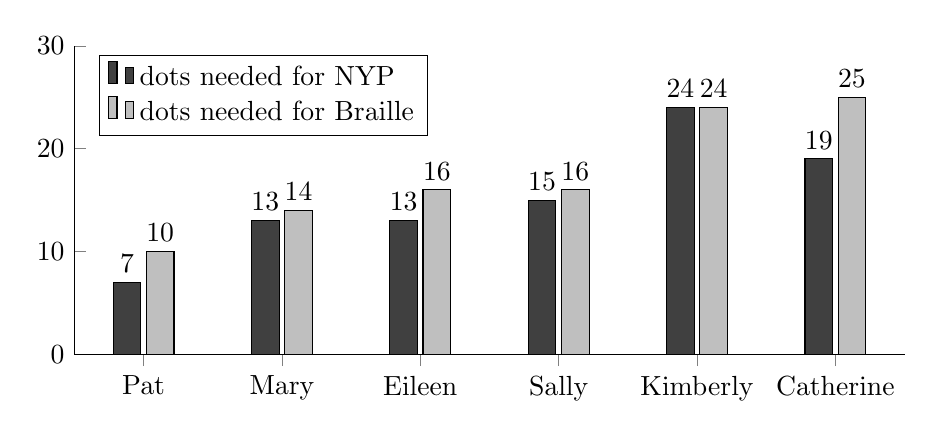
\begin{tikzpicture}
  \begin{axis}[ybar,
        axis lines*=left,
        symbolic x coords = {Pat,Mary,Eileen,Sally,Kimberly,Catherine},
        xtick=data,
        ymin=0,
        ymax=30,
        nodes near coords,
        width=\textwidth,
        height=5.5cm,
        bar width=1em,
        legend pos=north west,
        legend cell align=left
        ]
        \addplot [black,fill=black!75] coordinates {(Pat,7) (Mary,13) (Eileen,13) (Sally,15) (Kimberly,24) (Catherine,19)};
        \addlegendentry{dots needed for NYP}
        
        \addplot [black,fill=black!25] coordinates {(Pat,10) (Mary,14) (Eileen,16) (Sally,16) (Kimberly,24) (Catherine,25)};
        \addlegendentry{dots needed for Braille}
    \end{axis}
\end{tikzpicture}
\end{figure}

\noindent They also pointed out that NYP had a distinct series of capital letters, whereas Braille only had a “capital”\ punctuation mark. 

On the Braille side, experts such as Helen Keller wrote that the NYP capitalization system was unintuitive and confusing (“I have often mistaken \cmubdata{D} for \cmubdata{j}, \cmubdata{I} for \cmubdata{b} and \cmubdata{Y} for double \cmubdata{o} in signatures, and I waste time looking at initial letters over and over again”), and that using Braille allowed her to correspond with blind people from all over the world.

The following 12 words in NYP represent, \OlympiadRandomOrder{}, the names: \cmubdata{Ashley}, \cmubdata{Barb}, \cmubdata{Carl}, \cmubdata{Dave}, \cmubdata{Elena}, \cmubdata{Fred}, \cmubdata{Gerald}, \cmubdata{Heather}, \cmubdata{Ivan}, \cmubdata{Jack}, \cmubdata{Kathy}, \cmubdata{Lisa}. \\

\begin{multicols}{2}
\begin{enumerate}
    \item {\Large \boldmath$\begin{smallmatrix} 
    \bullet & \bullet & \bullet & \bullet \\  & & \bullet &
\end{smallmatrix}$\ \ $\begin{smallmatrix}
  \bullet & \bullet \\  & 
\end{smallmatrix}$\ \ $\begin{smallmatrix}
  \bullet & \bullet \\ \bullet & \bullet
\end{smallmatrix}$\ \ $\begin{smallmatrix}
  & \bullet &  \\ \bullet& & \bullet
\end{smallmatrix}$}

    \item {\Large \boldmath$\begin{smallmatrix} 
    \bullet &  &  &  \\  &\bullet&\bullet & \bullet 
\end{smallmatrix}$\ \ $\begin{smallmatrix}
  \bullet &  \\  \bullet& \bullet
\end{smallmatrix}$\ \ $\begin{smallmatrix}
  \bullet  \\ \,
\end{smallmatrix}$\ \ $\begin{smallmatrix}
  & \\ \bullet & \bullet
\end{smallmatrix}$\ \ $\begin{smallmatrix}
  \bullet & \bullet  \\ & 
\end{smallmatrix}$}

\item {\Large \boldmath$\begin{smallmatrix} 
    \bullet & \bullet & \bullet & \bullet \\ \bullet & &  &
\end{smallmatrix}$\ \ $\begin{smallmatrix}
  \bullet & & \bullet \\  & \bullet &
\end{smallmatrix}$\ \ $\begin{smallmatrix}
  \bullet & \bullet \\  & 
\end{smallmatrix}$\ \ $\begin{smallmatrix}
  &  \\ \bullet& \bullet
\end{smallmatrix}$}
    
\item {\Large \boldmath$\begin{smallmatrix} 
    \bullet & \bullet &  & \bullet \\  & & \bullet &
\end{smallmatrix}$\ \ $\begin{smallmatrix}
  \bullet & \bullet \\  & 
\end{smallmatrix}$\ \ $\begin{smallmatrix}
  & \bullet \\ \bullet & \bullet
\end{smallmatrix}$\ \ $\begin{smallmatrix}
  \bullet &  \\ \bullet& \bullet
\end{smallmatrix}$}

\item {\Large \boldmath$\begin{smallmatrix} 
    \bullet & \bullet & \bullet &  \\  &\bullet &  &\bullet
\end{smallmatrix}$\ \ $\begin{smallmatrix}
  \bullet & \bullet \\  & 
\end{smallmatrix}$\ \ $\begin{smallmatrix}
  \bullet & \bullet & \\  & & \bullet
\end{smallmatrix}$\ \ $\begin{smallmatrix}
  \bullet & \bullet & \bullet \\ & & \bullet
\end{smallmatrix}$}

\item {\Large \boldmath$\begin{smallmatrix} 
     &  & \bullet & \bullet \\ \bullet &\bullet & \bullet &
\end{smallmatrix}$\ \ $\begin{smallmatrix}
  \bullet  \\  \,
\end{smallmatrix}$\ \ $\begin{smallmatrix}
  & \bullet \\ \bullet & \bullet
\end{smallmatrix}$\ \ $\begin{smallmatrix}
  \bullet & \bullet  \\ & 
\end{smallmatrix}$\ \ $\begin{smallmatrix}
  \bullet &   \\ \bullet& \bullet
\end{smallmatrix}$\ \ $\begin{smallmatrix}
  \bullet & \bullet  \\ & \bullet
\end{smallmatrix}$}

\item {\Large \boldmath$\begin{smallmatrix} 
    \bullet &  & \bullet & \bullet \\ \bullet &\bullet&  &
\end{smallmatrix}$\ \ $\begin{smallmatrix}
  \bullet \\  \bullet
\end{smallmatrix}$\ \ $\begin{smallmatrix}
  \bullet & \\ & \bullet
\end{smallmatrix}$\ \ $\begin{smallmatrix}
  \bullet & \bullet  \\  & 
\end{smallmatrix}$}

\item {\Large \boldmath$\begin{smallmatrix} 
    \bullet & \bullet & \bullet &  \\  & &  &\bullet
\end{smallmatrix}$\ \ $\begin{smallmatrix}
  & \bullet \\  \bullet& \bullet
\end{smallmatrix}$\ \ $\begin{smallmatrix}
  \bullet \\ \,
\end{smallmatrix}$\ \ $\begin{smallmatrix}
  \bullet & \bullet \\ & \bullet
\end{smallmatrix}$}

\item {\Large \boldmath$\begin{smallmatrix} 
    & \bullet & \bullet & \bullet & \\  \bullet&\bullet & \bullet &
\end{smallmatrix}$\ \ $\begin{smallmatrix}
  \bullet \\  \, 
\end{smallmatrix}$\ \ $\begin{smallmatrix}
  \bullet & \bullet \\  & 
\end{smallmatrix}$\ \ $\begin{smallmatrix}
 \bullet  & \bullet  \\ \bullet& \bullet
\end{smallmatrix}$\ \ $\begin{smallmatrix}
 \bullet  \\ \,
\end{smallmatrix}$\ \ $\begin{smallmatrix}
  & \bullet  \\ \bullet& \bullet
\end{smallmatrix}$}

\item {\Large \boldmath$\begin{smallmatrix} 
    \bullet & \bullet & \bullet &  \\ \bullet & &  &\bullet
\end{smallmatrix}$\ \ $\begin{smallmatrix}
  \bullet & \bullet \\  & 
\end{smallmatrix}$\ \ $\begin{smallmatrix}
  & \bullet \\ \bullet & \bullet
\end{smallmatrix}$\ \ $\begin{smallmatrix}
  \bullet & \bullet & \bullet  \\ \bullet& & 
\end{smallmatrix}$}

\item {\Large \boldmath$\begin{smallmatrix} 
    \bullet & \bullet & & \\  & & \bullet & \bullet 
\end{smallmatrix}$\ \ $\begin{smallmatrix}
  & \bullet &  \\  \bullet & \bullet & \bullet
\end{smallmatrix}$\ \ $\begin{smallmatrix}
  \bullet & \\ \bullet & \bullet
\end{smallmatrix}$\ \ $\begin{smallmatrix}
  \bullet \\ \, 
\end{smallmatrix}$\ \ $\begin{smallmatrix}
  & \bullet &  \\ \bullet& & \bullet
\end{smallmatrix}$}

\item {\Large \boldmath$\begin{smallmatrix} 
    \bullet & \bullet & \bullet & \bullet \\  & \bullet & &
\end{smallmatrix}$\ \ $\begin{smallmatrix}
  \bullet & \bullet \\  & 
\end{smallmatrix}$\ \ $\begin{smallmatrix}
  \bullet & & \bullet \\ & \bullet &
\end{smallmatrix}$\ \ $\begin{smallmatrix}
  \bullet \\ \,
\end{smallmatrix}$}
\end{enumerate}
\end{multicols}

\begin{assgts}
\item \detcorr
\item Write in NYP: \cmubdata{Billy}, \cmubdata{Ethan}, \cmubdata{Iggie}, \cmubdata{Orson}, \cmubdata{Sasha}, \cmubdata{Tim}.
\end{assgts}
\end{problem}

\begin{problem}{\langnameLepcha}{\nameMChoudhury}{\LOYear{\PLOAbbr}{2015}}
Sikkim state in India has 11 official languages. Amongst these, ten are given below (the eleventh one is English) written in the Lepcha script, as well as in the Latin script:

\begin{center}
    \begin{tabular}{lc@{\hskip0.5in}lc}
        \cmubdata{nepaalii} & \lepchatext{\huge \charstack{\char"1C0D}{\char"1C2C}\char"1C0E\char"1C28\char"1C27\charstack{\char"1C1C}{\char"1C36}} & \cmubdata{newaar} & \lepchatext{\huge \charstack{\char"1C0D}{\char"1C2C}\charstack{\char"1C22}{\char"1C32}\char"1C28}  \\[0.3em]

        \cmubdata{lepchaa} & \lepchatext{\huge \charstack{\char"1C1C}{{\char"1C2C}{\char"1C31}}\char"1C06\char"1C28} & \cmubdata{raai} & \lepchatext{\huge \char"1C1B\char"1C28\char"1C27\char"1C23}  \\[0.3em]

        \cmubdata{sikkim} & \lepchatext{\huge \charstack{\char"1C0C}{{\char"1C2C}{\char"1C30}}\char"1C25\char"1C34\char"1C29\char"1C19\charstack{\char"1C00}{{\char"1C2C}{\char"1C36}}} & \cmubdata{gurung} & \lepchatext{\huge \char"1C03\char"1C2A\char"1C34\char"1C1B\char"1C2A}  \\[0.3em]

        \cmubdata{taamaang} & \lepchatext{\huge \char"1C0A\char"1C28\char"1C34\char"1C15\char"1C28} & \cmubdata{magar} & \lepchatext{\huge \char"1C15\charstack{\char"1C03}{\char"1C32}}  \\[0.3em]

        \cmubdata{liimbu} & \lepchatext{\huge \char"1C27
        \charstack{\charstack{\char"1C1C}{\char"1C2E}}{\raisebox{0.15em}{\char"1C36}}\char"1C13\char"1C2A} & \cmubdata{sunwaar} & \lepchatext{\huge \charstack{\char"1C20}{\char"1C30}\char"1C2A\charstack{\char"1C22}{\char"1C32}\char"1C28}  \\[0.3em]
    \end{tabular}
\end{center}

\begin{assgts}
\item One of the languages above has, in reality, two names, and its name written in the Latin script does not match the name written in the Lepcha script. Its name, transliterated from Lepcha, is \cmubdata{drenzoongkee}. Which language is this?
\item The Lepcha speakers, who call themselves \cmubdata{roong haagiit} (or, in the Lepcha script, \lepchatext{\char"1C34\char"1C29\char"1C1B\ \ \char"1C1D\char"1C28\char"1C27\charstack{\charstack{\char"1C03}{\char"1C33}}{\raisebox{0.15em}{\char"1C36}}}) are composed of four main distinct communities: \lepchatext{\charstack{\char"1C1B}{{\char"1C30}{\char"1C2C}}\char"1C34\char"1C29\char"1C19\char"1C15\char"1C2A}, \lepchatext{\charstack{\char"1C0A}{\char"1C2E}\char"1C28\char"1C34\char"1C20\char"1C28\char"1C15\char"1C2A}, \lepchatext{\char"1C27\char"1C1D\charstack{\char"1C1C}{\char"1C2E}\char"1C28\char"1C15\char"1C2A}, and \lepchatext{\char"1C29\char"1C0E\char"1C25\char"1C15\char"1C2A}. Transcribe these four community names into the Latin script.
\item Sikkim boasts the \cmubdata{Kaangchenzoonggaa}, the third highest peak in the world, which, in Tibetan, means \texttr{the five treasures of the high snow}. Transcribe the name of this peak in Lepcha.
\end{assgts}

\begin{tblsWarning}
Vowel doubling denotes length. \explainch{ch}; \explainng{ng}; \explainv{w}.
\end{tblsWarning}
\end{problem}

\begin{problem}{\langnameArabic\ -- \langnameHebrew}{\nameGParti}{\LOYear{\HKLOAbbr}{2020}}

Arabic and Hebrew are today two different, mutually unintelligible languages. However, they share both grammatical similarities and several lexical correspondences. Besides loanwords (mostly from Arabic to Hebrew) from different historical periods, scholars have identified over a thousand \textit{cognates} (words with a common etymological origin from Proto-Semitic, which is the partially re\-con\-structed common ancestor language spoken around 6,000 years ago).

The two lists below show pairs of cognates, but the pairs are mixed: Arabic on the left, and Hebrew on the right. The first match (1--A) is given for you.

% \begin{center}
    \begin{longtable}{>{\LARGE}crcrc}
        \arbtext{شمس} & 1. & $\xleftrightarrow{\hphantom{Indent}}$ & A. & \LARGE{{שׁמשׁ}}\\[0.3em]
        \arbtext{غضب} & 2. &  & B. & \LARGE{{כּלב}}\\[0.3em]
        \arbtext{ولد} & 3. &  & C. & \LARGE{{מלך}}\\[0.3em]
        \arbtext{أرض} & 4. &  & D. & \LARGE{{עבד}}\\[0.3em]
        \arbtext{بطن} & 5. &  & E. & \LARGE{{ארץ}}\\[0.3em]
        \arbtext{كلب} & 6. &  & F. & \LARGE{{עצב}}\\[0.3em]
        \arbtext{حبل} & 7. &  & G. & \LARGE{{קרן}}\\[0.3em]
        \arbtext{ملك} & 8. &  & H. & \LARGE{{ילד}}\\[0.3em]
        \arbtext{قرن} & 9. &  & I. & \LARGE{{חבל}}\\[0.3em]
        \arbtext{عبد} & 10. &  & J. & \LARGE{{בּטן}}\\[0.3em]
    \end{longtable}
% \end{center}

Thanks to regular and consistent sound changes, we have some easily identifiable patterns. Take for example the following eight words from the list above (transcribed in the Latin script):

\begin{table}[H]
\begin{tabular}{lll lll}
    \lsptoprule
    \langnameArabic & \langnameHebrew & Translation & \langnameArabic & \langnameHebrew & Translation \\
    \cmidrule(r){1-3}\cmidrule(l){4-6}
    \arabhebtr{kalb}{kelev}{dog} & \arabhebtr{shams}{shemesh}{sun} \\
    \arabhebtr{malik}{melekh}{king} & \arabhebtr{qarn}{qeren}{horn} \\
    \arabhebtr{'arḍ}{'erets}{land, earth} & \arabhebtr{ghaḍab}{\textsuperscript{ʕ}etsev}{anger, sadness} \\
    \arabhebtr{\textsuperscript{ʕ}abd}{\textsuperscript{ʕ}eved}{slave} & \arabhebtr{walad}{yeled}{child} \\
    \lspbottomrule
\end{tabular}
\end{table}

\begin{assgts}
    \item What is the transliteration (in both Arabic and Hebrew) of the two word pairs from the lists 1-10 and A-J not included in the table showing transliterations?
    \item The chart below shows a few letters in both scripts with their transliterations. Note that some letters may have different forms depending on the context they appear in. 
    
    \begin{description}[style=nextline]
    \item [\langnameHebrew:] ~ \\
        \begin{tabular}{|c|c|c|c|c|c|}
        \hline 
             \LARGE{{ר}} & \LARGE{{ץ / צ}} & \LARGE{{ע}} & \LARGE{{ן / נ}} & \LARGE{{ךּ / כּ}} & \LARGE{{י}} \\  \hline 
             (1)         & (2)             & (3)         & (4)             & \cmubdata{k}    & (5)         \\  \hline 
        \end{tabular}\medskip\\
        \begin{tabular}{|c|c|c|c|c|c|}
            \hline
             \LARGE{{ט}} & \LARGE{{ח}} & \LARGE{{ד}} & \LARGE{{ב}} & \LARGE{{בּ}} & \LARGE{{א}} \\\hline
             \cmubdata{t} & \cmubdata{ẖ}  & (6) & (7) & \cmubdata{b} & \cmubdata{'} (alef)\\\hline
        \end{tabular}    
    \item[\langnameArabic:] ~ \\
        \begin{tabular}{|@{\hskip0.2em}c@{\hskip0.2em}|c@{\hskip0.2em}|c@{\hskip0.2em}|c@{\hskip0.2em}|c@{\hskip0.2em}|}
        \hline 
            \arbtext{ـط} / \arbtext{ـطـ} / \arbtext{طـ} & \arbtext{ـر} / \arbtext{ر} & \arbtext{ـد} / \arbtext{د} & \arbtext{ـح} / \arbtext{ـحـ} / \arbtext{حـ} & \arbtext{ـب} / \arbtext{ـبـ} / \arbtext{بـ}  \\\hline 
            \cmubdata{ṭ} & (8) & (9) & \cmubdata{ḥ} & (10)  \\ \hline 
        \end{tabular}\medskip\\
        \begin{tabular}{|c@{\hskip0.2em}|@{\hskip0.2em}c@{\hskip0.2em}|c@{\hskip0.2em}|c@{\hskip0.2em}|c@{\hskip0.2em}|c@{\hskip0.2em}|}
        \hline 
            \arbtext{أ} & \arbtext{ـو} / \arbtext{و} & \arbtext{ـن} / \arbtext{ـنـ} / \arbtext{نـ} & \arbtext{ـل} / \arbtext{ـلـ} / \arbtext{لـ} & \arbtext{ـك} / \arbtext{ـكـ} / \arbtext{كـ} & \arbtext{ض} \\\hline 
            \cmubdata{'} (alif) & (11) & (12) & (13) & (14) & (15)  \\ \hline 
        \end{tabular}
\end{description}
    \item[] Fill in the gaps (1--15).
    
    \item Pair the matching cognates 2-10 and B-J from the first list (words transcribed in Arabic and Hebrew).
    \item If \texttr{thousand} in Arabic is \arbtext{ألف} and the final letter \cmubdata{f} in Hebrew is \mbox{ף}, what is the transliteration of {{אלף}} – also meaning \texttr{thousand} in Hebrew?
\end{assgts}

\begin{tblsWarning}
The apostrophe (') in both languages represents a glottal stop /ʔ/. In Arabic it is written by a \textit{hamza}, which often `sits' on top of an \textit{alif}; in Hebrew, it is represented by an \textit{alef} and often omitted in pronunciation. Here, you should just consider it a consonant and treat it like you would treat any other consonant!

The symbol \textsuperscript{ʕ} represents a voiced pharyngeal fricative /ʕ/, which is an odd sound made by contracting the muscles in the throat. It gives Arabic its unique flavour we can easily hear. In Modern Hebrew, it is silent and almost only ever appears in writing. Just think of it as an ordinary consonant!
\end{tblsWarning}

\end{problem}

\begin{problem}{\langnameJavanese}{\nameTHLee}{\LOYear{\NACLOAbbr}{2016}}
Here are some Javanese words in the Javanese script, Latin script, and their English translations:

\begin{center}
\begin{longtable}{rccc}
     \javaneseline{\javtext{\char"A9A5\char"A9BC\char"A99A\char"A98F\char"A9B6\char"A9A0\char"A9C0}}{penyakit}{disease}
     \javaneseline{\javtext{\char"A986\char"A981\ \char"A992\char"A9BF\char"A9B6\char"A9B1\char"A9C0}}{Inggris}{England}
     \javaneseline{\begin{tabular}{c}
          \includegraphics[width = 7em]{images/Java-stacked/3.png} 
     \end{tabular}}{traktor}{tractor}
     \javaneseline{\begin{tabular}{c}
          \includegraphics[width = 6.5em]{images/Java-stacked/4.png} 
     \end{tabular}}{panyumbang}{donor}
     \javaneseline{\begin{tabular}{c}
          \includegraphics[width = 8em]{images/Java-stacked/5.png} 
     \end{tabular}}{rembulan}{moon}
     \javaneseline{\begin{tabular}{c}
          \includegraphics[width = 6.5em]{images/Java-stacked/6.png} 
     \end{tabular}}{tansah}{always}
     \javaneseline{\javtext{\char"A984\char"A9BA\hspace{0.4em} \char"A9A9\char"A9AB\char"A9B6\char"A98F}}{Amérika}{America}
     \javaneseline{\javtext{\char"A994\char"A9BD\char"A9A7\char"A9B8\char"A9A0\char"A9C0}}{ngrebut}{to grab}
     \javaneseline{\javtext{\char"A9B2\char"A9B6\char"A9A7\char"A9B8\char"A9BA\hspace{0.65em}\char"A98F\char"A9B4\char"A9A0}}{ibukota}{capital}
     \javaneseline{\begin{tabular}{c}
          \includegraphics[width = 8em]{images/Java-stacked/10.png} 
     \end{tabular}}{Argentina}{Argentina}
     \javaneseline{\javtext{\char"A9B1\char"A9BD\char"A9BA\hspace{0.65em}\char"A994\char"A9BA\hspace{0.65em}\char"A994}}{srengéngé}{sun}
     \javaneseline{\begin{tabular}{c}
          \includegraphics[width = 6em]{images/Java-stacked/12.png} 
     \end{tabular}}{palsu}{false}
     \javaneseline{\javtext{\char"A989\char"A989\char"A981\char"A992\char"A9A4\char"A9C0}}{rerenggan}{decoration}
     \javaneseline{\javtext{\char"A9B2\char"A981\char"A9B1\char"A9AD\char"A9C0}}{angsal}{to acquire}
     \javaneseline{\javtext{\char"A9B2\hspace{-0.3em}\char"A9B6\hspace{0.5em}\char"A981\hspace{-0.2em}\char"A992\char"A9B6\char"A983}}{inggih}{yes}
     \javaneseline{\javtext{\char"A98F\char"A9BC\char"A989\char"A9A5\char"A9C0}}{\pbblank}{often}
     \javaneseline{\begin{tabular}{c}
          \includegraphics[width = 8em]{images/Java-stacked/17.png} 
     \end{tabular}}{\pbblank}{letter, script}
     \javaneseline{\begin{tabular}{c}
          \includegraphics[width = 6em]{images/Java-stacked/18.png} 
     \end{tabular}}{\pbblank}{to unload}
     \javaneseline{\begin{tabular}{c}
          \includegraphics[width = 8em]{images/Java-stacked/19.png} 
     \end{tabular}}{\pbblank}{to examine}
     \javaneseline{\javtext{\char"A9A9\char"A9B8\char"A9AB\char"A9B8\char"A994\char"A9BA\hspace{0.65em}\char"A98F}}{\pbblank}{to cancel}
     \javaneseline{\pbblank}{nyolong}{to steal}
     \javaneseline{\pbblank}{sepalih}{half}
     \javaneseline{\pbblank}{trengginas}{lively}
     \javaneseline{\pbblank}{Antartika}{Antarctica}
     \javaneseline{\pbblank}{Istanbul}{Istanbul}
\end{longtable}
\end{center}

\begin{assgts}
\item \fillblanks
\end{assgts}
\begin{tblsWarning} 
\cmubdata{ny} and \cmubdata{ng} are consonants; \cmubdata{é} is a vowel.
\end{tblsWarning}
\end{problem}

\begin{problem}{\langnameThai}{\nameSDmitrenko}{\LOYear{\MSKAbbr}{2001}}
Here are some Thai words written in the Thai script and their Latin transcriptions (together with their English translations) given \OlympiadRandomOrder{}:
\begin{enumerate}

    \begin{multicols}{5}
        \item \thaitext{หวาย}
        \item \thaitext{ท่าน}
        \item \thaitext{วาย}
        \item \thaitext{ว่าย}
        \item \thaitext{กาย}
        \item \thaitext{ทัน}
        \item \thaitext{กาว}
        \item \thaitext{ถาด}
        \item \thaitext{ถาก}
        \item \thaitext{วัย}
        \item \thaitext{หลาว}
        \item \thaitext{ทาน}
        \item \thaitext{หลัง}
        \item \thaitext{ลาว}
        \item[] \quad 
    \end{multicols}
\end{enumerate}

\begin{center}
    \begin{tabular}{rll@{\hskip1in}rll}
        A. & \pbsv{tʰà:k}{to clear (a field)} & H. & \pbsv{ka:w}{glue} \\[0.3em]
        B. & \pbsv{vâ:y}{to swim} & I. & \pbsv{la:w}{Laotian} \\[0.3em]
        C. & \pbsv{lǎ:w}{javelin} & J. & \pbsv{tʰâ:n}{you (formal)} \\[0.3em]
        D. & \pbsv{va:y}{to end} & K. & \pbsv{tʰa:n}{charity} \\[0.3em]
        E. & \pbsv{vǎ:y}{rattan} & L. & \pbsv{vay}{age} \\[0.3em]
        F. & \pbsv{tʰan}{to have time} & M. & \pbsv{tʰà:t}{tray} \\[0.3em]
        G. & \pbsv{lǎŋ}{back} & N. & \pbsv{ka:y}{body} \\[0.3em]
    \end{tabular}
\end{center}
\begin{assgts}
\item \detcorr
\item \taskWriteIn{\langnameThai}:

\begin{center}
    \begin{tabular}{rll@{\hskip1in}rll}
         15. & \pbsv{vǎ:n}{sweet} & 17. & \pbsv{tʰàk}{to knit} \\[0.3em] 
         16. & \pbsv{ya:ŋ}{rubber} & 18. & \pbsv{vâ:w}{kite} \\[0.3em] 
    \end{tabular}
\end{center}
\end{assgts}

\begin{tblsWarning}
A colon (\cmubdata{:}) after a vowel indicates length. The marks above vowels denote tones. This problem features four tones: medium (\cmubdata{a}), rising (\cmubdata{ǎ}), falling (\cmubdata{â}), low (\cmubdata{à}).

\cmubdata{tʰ} and \cmubdata{ŋ} are consonants.
\end{tblsWarning}

\end{problem}

\hypertarget{solutions-of-practice-problems}{%
\section{Solutions of practice problems}}

\begin{practiceproblemsolution}{2.5. \langnameArmenian}

\begin{solutions}[label=Solution 2.5\alph*]
    \item \cmubdata{Gortsaranayin}
    \item 7
    \item \cmubdata{Avtogortsaran} (the character resembling the letter S can be inferred to mean \cmubdata{t} from the title of the map, where the last word is \cmubdata{metropoliten}).
\end{solutions}

\end{practiceproblemsolution}

\pagebreak
\begin{practiceproblemsolution}{2.6. Ogham}

\begin{solutions}[label=Solution 2.6\alph*]
    \item \begin{enumerate}
        \begin{multicols}{7}
            \item B
            \item G
            \item D
            \item A
            \item F
            \item C
            \item E
        \end{multicols}
    \end{enumerate}
    \item \cmubdata{ta me i ngra leat} (in reality it is \cmubdata{Tá mé i ngrá leat}).
\end{solutions}

\rules

We can classify the characters depending on the number of dots or lines as well as their position or direction (vertical or diagonal, above or below the horizontal line):

\begin{table}[H]
    \begin{tabular}{l *5{c}}
    \lsptoprule
 & 1 line & 2 lines & 3 lines & 4 lines & 5 lines \\\midrule
vertical, below & & \cmubdata{l} &  & \cmubdata{s} & \cmubdata{n} \\
vertical, above & \cmubdata{h} &  & \cmubdata{t} & \cmubdata{c} &  \\
diagonal & \cmubdata{m} & \cmubdata{g} &  &  & \cmubdata{r} \\
dots & \cmubdata{a} & \cmubdata{o} &  & \cmubdata{e} & \cmubdata{i}\\
\lspbottomrule
\end{tabular}
\end{table}

The accents are not marked (\cmubdata{á} = \cmubdata{a}).
\end{practiceproblemsolution}



\begin{practiceproblemsolution}{2.7. New York Point}

\begin{solutions}[label=Solution 2.7\alph*]
    \item \begin{enumerate}\largerpage[2]

    \begin{multicols}{4}
        \item \cmubdata{Kathy}
        \item \cmubdata{Elena}
        \item \cmubdata{Ivan}
        \item \cmubdata{Carl}
        \item \cmubdata{Jack}
        \item \cmubdata{Gerald}
        \item \cmubdata{Lisa}
        \item \cmubdata{Fred}
        \item \cmubdata{Heather}
        \item \cmubdata{Barb}
        \item \cmubdata{Ashley}
        \item \cmubdata{Dave}
    \end{multicols}
    \end{enumerate}
    \item
    \begin{tabular}[t]{lcl}
         \cmubdata{Billy} & -- & {\Large \boldmath$\begin{smallmatrix}
    \bullet & \bullet & \bullet &  \\  \bullet& &  &\bullet
\end{smallmatrix}$\ \ \boldmath$\begin{smallmatrix}
    \bullet \\  \bullet\end{smallmatrix}$\ \ \boldmath$\begin{smallmatrix}
    \bullet &\\  \bullet&\bullet\end{smallmatrix}$\ \ \boldmath$\begin{smallmatrix}
    \bullet & \\  \bullet&\bullet\end{smallmatrix}$\ \ \boldmath$\begin{smallmatrix}
    &\bullet& \\  \bullet&&\bullet\end{smallmatrix}$}\\ [0.5em]
         \cmubdata{Ethan} & -- & {\Large \boldmath$\begin{smallmatrix}
    \bullet &  &  &  \\  &\bullet & \bullet &\bullet
\end{smallmatrix}$\ \ \boldmath$\begin{smallmatrix}
    \bullet &\bullet  \\  \bullet&\bullet\end{smallmatrix}$\ \ \boldmath$\begin{smallmatrix}
    \bullet&\bullet \\  &\end{smallmatrix}$\ \ \boldmath$\begin{smallmatrix}
    & \\  \bullet&\bullet\end{smallmatrix}$}\\[0.5em]
         \cmubdata{Iggie} & -- & {\Large \boldmath$\begin{smallmatrix}
    \bullet & \bullet & \bullet & \bullet \\  \bullet &&
\end{smallmatrix}$\ \ \boldmath$\begin{smallmatrix}
    &&\bullet \\ \bullet&\bullet&\bullet\end{smallmatrix}$\ \ \boldmath$\begin{smallmatrix}
    &&\bullet \\ \bullet&\bullet&\bullet\end{smallmatrix}$\ \ \boldmath$\begin{smallmatrix}
    \bullet \\  \bullet\end{smallmatrix}$\ \ \boldmath$\begin{smallmatrix}
    \bullet \\  \end{smallmatrix}$}\\[0.5em]
    \cmubdata{Orson} & -- & {\Large\boldmath$\begin{smallmatrix}
    &\bullet&& \\  \bullet&&\bullet&\bullet\end{smallmatrix}$\ \ \boldmath$\begin{smallmatrix}
    &\bullet \\  \bullet&\bullet\end{smallmatrix}$\ \ \boldmath$\begin{smallmatrix}
    \bullet& \\  &\bullet\end{smallmatrix}$\ \ \boldmath$\begin{smallmatrix}
    &\bullet \\  \bullet&\end{smallmatrix}$\ \ \boldmath$\begin{smallmatrix}
    &\\\bullet&\bullet\end{smallmatrix}$}\\[0.5em]
         \cmubdata{Sasha} & -- & {\Large \boldmath$\begin{smallmatrix}
    \bullet && \bullet & \bullet  \\  &\bullet &  &
\end{smallmatrix}$\ \ \boldmath$\begin{smallmatrix}
    \bullet&\bullet \\  &\end{smallmatrix}$\ \ \boldmath$\begin{smallmatrix}
    &\bullet& \\ \bullet&\bullet&\bullet\end{smallmatrix}$\ \ \boldmath$\begin{smallmatrix}
    \bullet&\bullet \\  &\end{smallmatrix}$}\\[0.5em]
         \cmubdata{Tim} & -- & {\Large \boldmath$\begin{smallmatrix}
    & \bullet & \bullet & \bullet  \\  \bullet &&  &
\end{smallmatrix}$\ \ \boldmath$\begin{smallmatrix}
    \bullet \\  \bullet\end{smallmatrix}$\ \ \boldmath$\begin{smallmatrix}
    \bullet&\bullet \\  \bullet&\end{smallmatrix}$}\\
    \end{tabular}
\end{solutions}

\rules

Forming the capital letter: all capital letters are four columns long and are formed by appending dots to the lowercase letter until it is four columns long, according to the following pattern:

\begin{itemize}
    \item If the last column of the lowercase letter has a dot in the upper row, add the extra dots on the lower row.
    \item If the last column of the lowercase letter has a dot in the lower row or both dots, add the extra dots on the upper row.
\end{itemize}
\end{practiceproblemsolution}

\begin{discussion}
\begin{sloppypar}
Figuring out the character for \cmubdata{o}: in the introduction it is mentioned that \cmubdata{Y} ({\Large \boldmath$\begin{smallmatrix}
    &\bullet&&\bullet&  \\  \bullet&&\bullet&
\end{smallmatrix}$}) can be mistaken for a double \cmubdata{o}, and \cmubdata{Y} is formed by the same pattern repeated twice, so that pattern must represent the letter \cmubdata{o} ({\Large \boldmath$\begin{smallmatrix} 
   & \bullet  \\  \bullet& 
\end{smallmatrix}$}).
\end{sloppypar}

Figuring out the characters for \cmubdata{t} and \cmubdata{m}: based on the graph given in the introduction, we can deduce that \cmubdata{t} must contain a single dot (\cmubdata{Pat} has seven dots, \cmubdata{a} is two dots and \cmubdata{P}, since it is uppercase, must have at least four dots). Since we already know that \cmubdata{e} is {\Large \boldmath$\begin{smallmatrix}
    \bullet  \\   
\end{smallmatrix}$}, \cmubdata{t} can only be {\Large \boldmath$\begin{smallmatrix} 
     \\  \bullet 
\end{smallmatrix}$}.

From the graph, we deduce that \cmubdata{M} has five dots and \cmubdata{m} three, therefore the three dots must be distributed on only two columns (since two columns are needed for the extra dots to form the uppercase). There are four options ({\Large \boldmath$\begin{smallmatrix}
    &\bullet  \\  \bullet&\bullet 
\end{smallmatrix}$}, {\Large \boldmath$\begin{smallmatrix} 
    \bullet&\bullet  \\  \bullet &
\end{smallmatrix}$} , {\Large \boldmath$\begin{smallmatrix} 
    \bullet&  \\  \bullet &\bullet
\end{smallmatrix}$} , {\Large \boldmath$\begin{smallmatrix} 
    \bullet&\bullet  \\  &\bullet 
\end{smallmatrix}$}). Since three of the characters are already used ({\Large \boldmath$\begin{smallmatrix} 
    &\bullet  \\  \bullet&\bullet 
\end{smallmatrix}$} = \cmubdata{r}, {\Large \boldmath$\begin{smallmatrix} 
    \bullet&  \\  \bullet &\bullet
\end{smallmatrix}$} = \cmubdata{l}, {\Large \boldmath$\begin{smallmatrix} 
    \bullet&\bullet  \\  &\bullet 
\end{smallmatrix}$} = \cmubdata{d}), there is only one option left to place the dots ({\Large \boldmath$\begin{smallmatrix} 
    \bullet&\bullet  \\  \bullet &
\end{smallmatrix}$}) such as the final pattern does not coincide with other letters.
\end{discussion}


\begin{practiceproblemsolution}{2.8. \langnameLepcha}

\begin{solutions}[label=Solution 2.8\alph*]
    \item Sikkim language
    \item \cmubdata{renzoongmu} \hfill \cmubdata{taamsaangmu} \hfill \cmubdata{hilaammu} \hfill \cmubdata{proomu}
    \item \lepchatext{\char"1C34\char"1C00\char"1C28\charstack{\char"1C06}{{\char"1C2C}{\char"1C30}}\char"1C34\char"1C29\char"1C19\char"1C03\char"1C28}
\end{solutions}

\rules
\begin{itemize}
    \item Abugida script, left-to-right.
    \item Consonants at the beginning of the syllable:

    \begin{center}
        \begin{tabular}{cccccccc}
            \lepchatext{\char"1C23} & \lepchatext{\char"1C13} & \lepchatext{\char"1C0C} & \lepchatext{\char"1C03} & \lepchatext{\char"1C1D} & \lepchatext{\char"1C06} & \lepchatext{\char"1C00} & \lepchatext{\char"1C1C} \\
            $\varnothing$ & \cmubdata{b} & \cmubdata{d} & \cmubdata{g} & \cmubdata{h} & \cmubdata{ch} & \cmubdata{k} & \cmubdata{l}\\\addlinespace
            \lepchatext{\char"1C15} & \lepchatext{\char"1C0D} & \lepchatext{\char"1C0E} & \lepchatext{\char"1C1B} & \lepchatext{\char"1C20} & \lepchatext{\char"1C0A} & \lepchatext{\char"1C22} & \lepchatext{\char"1C19} \\
            \cmubdata{m} & \cmubdata{n} & \cmubdata{p} & \cmubdata{r} & \cmubdata{s} & \cmubdata{t} & \cmubdata{w} & \cmubdata{z}\\
        \end{tabular}
    \end{center}

    \item Vowels are marked by diacritics. The default vowel is \cmubdata{a}.

    \begin{center}
        \begin{tabular}{cccccccc}
            \lepchatext{\char"25CC} & \lepchatext{\char"25CC\char"1C28} & \lepchatext{\charstack{\char"25CC}{\char"1C2C}} & \lepchatext{\charstack{\char"25CC}{{\char"1C2C}{\char"1C36}}} & \lepchatext{\char"1C27\char"25CC} & \lepchatext{\char"1C27\charstack{\char"25CC}{\char"1C36}} & \lepchatext{\char"1C29\char"25CC} & \lepchatext{\char"25CC\char"1C2A} \\
            \cmubdata{a} & \cmubdata{aa} & \cmubdata{e} & \cmubdata{ee} & \cmubdata{i} & \cmubdata{ii} & \cmubdata{oo} & \cmubdata{u}\\
        \end{tabular}
    \end{center}

    \item Consonants at the end of the syllable (codas) are also marked by diacritics:

    \begin{center}
        \begin{tabular}{cccccc}
            \lepchatext{\charstack{\char"25CC}{\char"1C2E}} & \lepchatext{\charstack{\char"25CC}{\char"1C30}} &  \lepchatext{\char"1C34\char"25CC} & \lepchatext{\charstack{\char"25CC}{\char"1C31}} & \lepchatext{\charstack{\char"25CC}{\char"1C32}} & \lepchatext{\charstack{\char"25CC}{\char"1C33}} \\
            \cmubdata{-m} & \cmubdata{-n} & \cmubdata{-ng} & \cmubdata{-p} & \cmubdata{-r} & \cmubdata{-t}\\
        \end{tabular}
    \end{center}
    \item If the syllable onset has the structure $C$\cmubdata{r}, that \cmubdata{r} is marked as \lepchatext{\char"25CC\char"1C25}. Compare:

    \begin{center}
        \begin{tabular}{ccc}
             \lepchatext{\char"1C00\char"1C25} & \lepchatext{\charstack{\char"1C00}{\char"1C32}} & \lepchatext{\charstack{\char"1C00}{\char"1C32}\char"1C25} \\
             \cmubdata{k\textbf{r}a} & \cmubdata{ka\textbf{r}} & \cmubdata{k\textbf{r}a\textbf{r}}
        \end{tabular}
    \end{center}
\end{itemize}
\end{practiceproblemsolution}


\begin{practiceproblemsolution}{2.9. Arabic and Hebrew}\largerpage[1.5]

\begin{solutions}[label=Solution 2.9\alph*]
    \item \cmubdata{ḥabl} \rightarrow\ \cmubdata{ẖevel} \\ \cmubdata{baṭn} \rightarrow\ \cmubdata{beten}
\end{solutions}

    \note{In Hebrew all vowels shown are \cmubdata{e}. In Arabic it is impossible to deduce the vowels based on the data, so alternative versions are also accepted (such as \cmubdata{ḥabal} or \cmubdata{ḥabil}).}
    
\begin{solutions}[label=Solution 2.9\alph*, resume]
    \item \largerpage
    \begin{multicols}{3}
    \begin{enumerate}[label = (\arabic*)]
            \item \cmubdata{r}
            \item \cmubdata{ts}
            \item \cmubdata{\textsuperscript{ʕ}} (ayin)
            \item \cmubdata{n}
            \item \cmubdata{y}
            \item \cmubdata{d}
            \item \cmubdata{v}
            \item \cmubdata{r}
            \item \cmubdata{d}
            \item \cmubdata{b}
            \item \cmubdata{w}
            \item \cmubdata{n}
            \item \cmubdata{l}
            \item \cmubdata{k}
            \item \cmubdata{ḍ}
        \end{enumerate}
    \end{multicols}
    \item \begin{enumerate}
        \begin{multicols}{5}
            \item A
            \item F
            \item H
            \item E
            \item J
            \item B
            \item I
            \item C
            \item G
            \item D
        \end{multicols}
    \end{enumerate}
    \item \cmubdata{'elef}
\end{solutions}

\end{practiceproblemsolution}
\pagebreak
\begin{practiceproblemsolution}{2.10. \langnameJavanese}

\begin{solutions}[label=Solution 2.10\alph*]
    \item
    \begin{enumerate}[label = (\arabic*)]

    \begin{multicols}{2}
        \item \cmubdata{kerep}
        \item \cmubdata{aksara}
        \item \cmubdata{mbongkar}
        \item \cmubdata{mrikso}
        \item \cmubdata{murungaké}
        \item \javtext{\char"A9BA\hspace{0.65em}\char"A99A\char"A9B4\char"A9BA\hspace{0.65em}\char"A9AD\char"A981\char"A9B4}
        \item \javtext{\char"A9B1\char"A9BC\char"A9A5\char"A9AD\char"A9B6\char"A983}
        \item \javtext{\char"A9A0\char"A9BD\char"A981\char"A992\char"A9B6\char"A9A4\char"A9B1\char"A9C0}
        \item \begin{tabular}{@{}l@{}}
             \includegraphics[width = 9em]{images/Java-stacked/sol9.png}
        \end{tabular}
        \item \begin{tabular}{@{}l@{}}
             \includegraphics[width = 9em]{images/Java-stacked/sol10.png}
        \end{tabular}
    \end{multicols}
    \end{enumerate}
\end{solutions}

\rules
\begin{itemize}
    \item Abugida script, left-to-right, with the default vowel \cmubdata{a}.
    \item Syllables have the structure $C_1(C_2)V(C_3)$, taking into account the following syllabification rules:
    \begin{itemize}

        \item $...VC^aC^bV... \rightarrow\ ...VC^a_3-C^b_1V...$ if $C^a$ is \cmubdata{ng}, \cmubdata{h}, or \cmubdata{r};
        \item $...VC^aC^bV... \rightarrow\ ...V-C^a_1C^b_1V...$ otherwise;
    \end{itemize}
    \item $C_1$

    \begin{center}
        \begin{tabular}{ccccccc}
            \javtext{\char"A9B2} & \javtext{\char"A9A7} & \javtext{\char"A992} & \javtext{\char"A98F} & \javtext{\char"A9AD} & \javtext{\char"A9A9} & \javtext{\char"A9A4} \\
            $\varnothing$ & \cmubdata{b} & \cmubdata{g} & \cmubdata{k} & \cmubdata{l} & \cmubdata{m} & \cmubdata{n} \\ &&&&&&\\

            \javtext{\char"A994} & \javtext{\char"A99A} & \javtext{\char"A9A5} & \javtext{\char"A9AB} & \javtext{\char"A9B1} & \javtext{\char"A9A0} &  \\
            \cmubdata{ng} &\cmubdata{ny} & \cmubdata{p} & \cmubdata{r} & \cmubdata{s} & \cmubdata{t} &  \\
        \end{tabular}
    \end{center}
    
\end{itemize}\largerpage[1.5]
    \note{The combination \cmubdata{re} has its own character: \javtext{\char"A989}}
\begin{itemize}
    
    \item The vowel change is shown using diacritics:

    \begin{center}
        \begin{tabular}{cccccc}
            \javtext{\char"25CC} & \javtext{\char"25CC\char"A9BC} & \javtext{\char"A9BA\hspace{0.6em}\char"25CC} & \javtext{\char"25CC\char"A9B6} & \javtext{\char"A9BA\hspace{0.6em}\char"25CC\char"A9B4} & \javtext{\char"25CC\char"A9B8}    \\
            \cmubdata{$C$a} & \cmubdata{$C$e} & \cmubdata{$C$é} & \cmubdata{$C$i} & \cmubdata{$C$o} & \cmubdata{$C$u}\\
        \end{tabular}
    \end{center}
    
    \item $C_2$:\footnote{In fact, this special form of the consonant marks the fact that the vowel of the preceding consonant is deleted.}

    \begin{center}
        \begin{tabular}{ccccc}
              \begin{tabular}{@{}c@{}}
                \includegraphics[width=2em]{images/Java-stacked/b-stack.png}
              \end{tabular} & \javtext{\char"25CC\char"A9BF} & \javtext{\char"25CC\char"A9BD} & \begin{tabular}{@{}c@{}}
                \includegraphics[width=3em]{images/Java-stacked/s-stack.png}
              \end{tabular} & \begin{tabular}{@{}c@{}}
                \includegraphics[width=2em]{images/Java-stacked/t-stack.png}
              \end{tabular}
              \\
             \cmubdata{b} & \hphantom{abc}\cmubdata{r}\hphantom{abc} & \cmubdata{re} & \cmubdata{s} & \cmubdata{t}
        \end{tabular}
    \end{center}
    \item $C_3$:

    \begin{center}
        \begin{tabular}{cccc}
            \javtext{\char"25CC\char"A981} & \javtext{\char"25CC\char"A983} & \javtext{\char"25CC\char"A982} & \javtext{C\char"A9C0}\\
            \cmubdata{ng} & \cmubdata{h} & \cmubdata{r} & else (\cmubdata{C})\footnotemark{}\\
        \end{tabular} \footnotetext{This is basically the vowel-removing mark, showing that the previous consonant does not have a vowel.}
    \end{center}
    \item Special characters for capital letters:

    \begin{center}
        \begin{tabular}{cc}
              \javtext{\char"A984} & \javtext{\char"A986}
              \\
             \cmubdata{A} & \cmubdata{I}
        \end{tabular}
    \end{center}
\end{itemize}

\end{practiceproblemsolution}

\begin{practiceproblemsolution}{2.11. \langnameThai}

\begin{solutions}[label=Solution 2.11\alph*]
    \item \begin{enumerate}

        \begin{multicols}{7}
            \item E
            \item J
            \item D
            \item B
            \item N
            \item F
            \item H
            \item M
            \item A
            \item L
            \item C
            \item K
            \item G
            \item I
        \end{multicols}
    \end{enumerate}
    \item \begin{enumerate}[resume]

        \begin{multicols}{4}
            \item \thaitext{หวาน}
            \item \thaitext{ยาง}
            \item \thaitext{ถัก}
            \item \thaitext{ว่าว}
        \end{multicols}
        \end{enumerate}
\end{solutions}

\rules
\begin{itemize}
    \item Writing direction from left to right.
    \item The character \thaitext{ว} represents two consonants: \cmubdata{v}, if in the beginning of the word; and \cmubdata{w}, if at the end of the word.
    \item The sound \cmubdata{t\textsuperscript{h}} corresponds to two Thai characters: \thaitext{ท} and \thaitext{ถ}. The latter is used to mark the low tone.
    \item Vowels: \cmubdata{a} = \thaitext{\char"25CC\char"0E31} (placed on the first consonant), \cmubdata{a:} = \thaitext{า}
    \item Tone:
    \begin{itemize}

        \item Medium -- default tone (unmarked);
        \item Rising -- \thaitext{ห} placed at the beginning of the word;
        \item Falling -- \thaitext{\char"25CC\char"0E48} placed on the first consonant;
        \item Low -- appears only in words starting with \cmubdata{tʰ}. In this case, the tone is marked by using the character \thaitext{ถ} to mark the consonant \cmubdata{tʰ} (rather than \thaitext{ท}).
    \end{itemize}
\end{itemize}
\end{practiceproblemsolution}

\begin{discussion}

The way that the Thai writing system represents tone is very complex. To know which tone to pronounce the syllable with, we need to know the initial consonant and the type of syllable. Initial consonants are split into three classes: low, medium (mid), and high, while the syllables are either ``live" (ending in \cmubdata{n}, \cmubdata{m}, \cmubdata{ŋ}, \cmubdata{w}, \cmubdata{y}) or ``dead" (ending in \cmubdata{p}, \cmubdata{t}, \cmubdata{k}). Moreover, there are some diacritics which may be added to further modify the tone. The following table details the rules relevant to the data in the problem:

\begin{table}[H]
    \begin{tabular}{ccccc}
    \lsptoprule
                 &               & \multicolumn{3}{c}{Type of first consonant} \\\cmidrule(lr){3-5}
     Diacritics  & Syllable type & \textit{low} & \textit{mid} & \textit{high} \\ \midrule 
    no mark      & \textit{live}         & medium (\cmubdata{a}) & medium (\cmubdata{a}) & rising (\cmubdata{\v{a}}) \\
    no mark      & \textit{dead}         & * & low (\cmubdata{à}) & low (\cmubdata{à}) \\  
    \thaitext{\char"25CC\char"0E48} & \textit{live}/\textit{dead}   & falling (\cmubdata{â}) & low (\cmubdata{à})   & low (\cmubdata{à})\\
     \lspbottomrule
    \end{tabular}
\footnotetext{* The choice of tone further depends on the vowel length: if the vowel is long, the syllable will have falling (\cmubdata{â}) tone; if the vowel is short, the syllable will have high (\cmubdata{á}) tone.}
\end{table}


Most words in the problem start with \textit{low} consonants (\thaitext{ล}, \thaitext{ท}, \thaitext{ว}, \thaitext{ล}). There is a single \textit{mid} consonant at the beginning of the words (\cmubdata{k} = \thaitext{ก}), but, since this one only appears in \textit{live} syllables, its tone is identical to that of a syllable starting with a \textit{low} consonant.

Most Thai consonants have two forms: a low form and a high form (in the problem we have the consonant \cmubdata{tʰ}, which, in its low form, is written as \thaitext{ท}, while in its high form becomes \thaitext{ถ}). If some consonants do not have two different characters to differentiate between low and high, a low consonant can become high by adding the character \thaitext{ห} before it (the character represents the high consonant \cmubdata{h}, but it is not pronounced).

Based on this information, the rules in our problem can be explained as follows:

\begin{itemize}
    \item the default tone is the medium one because most of the words contain live syllables and start with a low or mid consonant.
    \item the falling tone is shown by the diacritic \thaitext{\char"25CC\char"0E48} and by the fact that these syllables all start with a low consonant (otherwise they would have a low tone).
    \item the character \thaitext{ถ} at the beginning of the word changes the tone to low because the syllable is dead (it is the only occurrence of a dead syllables in the problem) and the first consonant is high.
    \item the rising tone is shown by adding the character \thaitext{ห} at the beginning of the word since it will transform the initial consonant from low to high.
\end{itemize}
\end{discussion}


\nocite{Coulmas1999, Coulmas2003, Cruttenden2021, DanielsBright1996, Haarmann2004, Robinson1999}
% \printbibliography[heading=FurtherReading]
\FurtherReadingBox{}
\end{refsection}


% \begin{enumerate}[{label=[\arabic{*}]}]
%     \item Coulmas, Florian. “The Blackwell encyclopedia of writing systems.”\ \textit{Wiley-Blackwell}, New York (1999).
%     \item Coulmas, Florian. “Writing systems. An introduction.”\ \textit{Cambridge University Press}, Cambridge (2003).
%     \item Cruttenden, Alan. “Writing systems and phonetics.”\ \textit{Routledge}, London (2021).
%     \item Daniels, Peter T. and Bright, William. “The world's writing systems.”\ \textit{Oxford University Press}, Oxford (1996).
%     \item Haarmann, Harald. “Geschichte der Schrift.”\ \textit{C. H. Beck}, München (2004).
%     \item Robinson, Andrew. “The story of writing.”\ \textit{Thames \& Hudson}, New York (1999).
% \end{enumerate}
 
\begin{refsection}
\hypertarget{phonetics}{%
\chapter{Phonetics}\label{chap-phonetics}}

\section{Introduction}

The field of phonetics is concerned with how speakers of different languages make the sounds of their speech (\textit{production}, or \textit{articulation}), and also with how they are heard by listeners (\textit{perception}; this is sometimes known as \textit{auditory phonetics}). Many linguistics problems will involve phenomena of \textit{phonology} – for now, we can define these as changes of sounds that depend on the structure of words. We will see many examples of these in \chapref{chap-phonology}. Before we do so, it is useful to look at the different types of sound, and the ways in which they are classified, in order to understand these types of change. 

In this chapter (and indeed throughout the book), we will use a notation system called the International Phonetic Alphabet (IPA). This is an alphabetic writing system, formed primarily of Latin characters and symbols derived therefrom and developed in order to make it possible to transcribe any word, from any spoken language, using this single set of conventions. Thus, each sound will have its own notation.

Writing down the sounds of a language is referred to as (phonetic) \textit{transcription}. To distinguish words that are transcribed from how they are represented in spelling, we often use square brackets (as in [tʰɹənsˈkɹɪp̚ʃn̩]) or slashes (as in /trænsˈkripʃən/), both corresponding to the spelling \cmubdata{transcription}. The precise difference between the two kinds of transcription shown here is not that important; very roughly, slashes are generally used for a kind of notation that only aims to differentiate the sounds found in that specific language (and thus omit some detail), while square brackets tend to contain quite \textit{narrow} transcriptions, which contain a lot of specific information. For example, the sound usually written as /r/ can, in fact, be pronounced differently in different languages, and those differences will be reflected in narrower transcriptions: in English, it can be represented as [ɹ] (for instance, in many dialects of England), [ɻ] (in North America or Northern Ireland), or [ɾ] (in Scotland); in Romanian, it is generally [r], and in French or German it is usually [ʁ]. Narrow transcriptions aim to reflect this detail that depends on each language, but as often as not we only need to worry about the broad outlines of the system and will just use /r/ for all of these sounds, since most languages have only one type of \cmubdata{r}. This distinction rarely matters in practice for solving linguistics problems.

\section{Classification of sounds}

Probably the most fundamental sound distinction that we need to keep in mind is the difference between vowels and consonants. The basic characteristic of vowels is that when we pronounce them, the air coming up from the lungs does not meet any obstacle (or, as we sometimes say, there is no constriction, either total or partial) in the vocal tract. Conversely, consonants are formed with some kind of obstacle, or \textit{stricture}.

\subsection{Consonants}

We can describe most consonants with reference to three main characteristics, which are referred to as \textit{place of articulation}, \textit{manner of articulation}, and \textit{voicing}. (“Articulation” is just what we call the movements involved when we make the different sounds of speech.)

\subsubsection{Place of articulation}

This describes where in the vocal tract the main constriction is located, i.e., what organs are primarily involved in the articulation of each consonant. Going from front (the lips) to back (the back of the throat), we can identify the following places of articulation for consonants:\footnote{A diagram of the vocal tract can be found on page 7 of the International Phonetic Association's \textit{Handbook of the International Phonetic Association}, published by Cambridge University Press in 1999.}

\begin{itemize}
    \item \textsc{Labial}, in which the lips are involved. In English, these are:
    \begin{itemize}

        \item \textsc{Bilabial} consonants, produced using both lips (\textit{bi-} = `two', \textit{labium} = `lip' \Rightarrow\ \texttr{two lips}): [{b}], [{p}], [{m}];
        \item \textsc{Labiodental} consonants (\textit{labium}, \textit{dental} = `tooth' \Rightarrow\ the lower lip and the upper teeth): [{f}], [{v}];
    \end{itemize}
    \item \textsc{Coronal}, pronounced by using the tip of the tongue:
    \begin{itemize}

        \item \textsc{(Inter)dental} consonants (\textit{inter} = `between', \textit{dental} \Rightarrow\ the tongue is placed between, or just on, the teeth) – [{θ}] (\cmubdata{th} in \cmubdata{thin}), [{ð}] (\cmubdata{th} in \cmubdata{that});
        \item \textsc{Alveolar} consonants (the tip of the tongue is placed on or near the alveolar ridge, the little protrusion just behind the upper teeth) – in English, [{t}], [{d}], [{s}], [{z}], [{n}], [{l}] are all usually alveolar, as is [{r}] in some languages other than English;\footnote{In most linguistics problems, the sound [{r}] is treated as an alveolar sound, unless the footnotes state differently.}
        \item \textsc{Post-alveolar} consonants (\textit{post} = ‘after’\ \Rightarrow\ the tongue is placed further behind than the alveolar ridge) – [{ʃ}] (\cmubdata{sh} in \cmubdata{shop}), [{ʒ}] (\cmubdata{s} in \cmubdata{vision}), [{tʃ}] (\cmubdata{ch} in \cmubdata{church}), [{dʒ}] (\cmubdata{j} in \cmubdata{jam}); in many varieties of English, [ɹ] is also post-alveolar;
    \end{itemize}
    \item \textsc{Dorsal} consonants, articulated primarily using the blade of the tongue:
    \begin{itemize}

        \item \textsc{Palatal} consonants (the tongue is placed against the hard palate of the oral cavity): one example from English is [{j}] (note that in the IPA this symbol refers to the \cmubdata{y} of \cmubdata{yellow}, not the \cmubdata{j} of \cmubdata{jam}!). Other palatal consonants are [{c}] (similar to \cmubdata{cc} in \cmubdata{accute}, but not as the \cmubdata{c} in \cmubdata{cat}), [{ɟ}] (similar to \cmubdata{g} in \cmubdata{geese}), [{ɲ}] (\cmubdata{ni} in \cmubdata{onion}), [{ʎ}] (as in Italian \cmubdata{figlio}, or in English \cmubdata{mi\textbf{lli}on});
        \item \textsc{Velar} consonants (the back of the tongue is placed against the soft palate, also known as the velum) – [{k}] (\cmubdata{c} in \cmubdata{cat}), [{ɡ}], [{ŋ}] (\cmubdata{ng} in \cmubdata{king}), [{x}] (as in Scottish \cmubdata{loch} or German \cmubdata{Bach});
    \end{itemize}
    \item \textsc{Glottal} consonants, which generally lack any constriction in the mouth, but some noise is created as air passes through the vocal folds (the glottis is the gap between the two vocal folds) – [{h}] and the glottal stop, written [{ʔ}] and heard in \cmubdata{uh-oh}, or, for some speakers, in the middle of words like \cmubdata{butter}. (Pronouncing \cmubdata{butter} with a glottal stop is sometimes called “dropping one's t's”, but that is clearly wrong: the \cmubdata{t} isn't dropped, it's just pronounced differently!)
\end{itemize}

These are the main places of articulation we encounter, but in the world's languages, there are quite a few more (\textit{alveolo-palatal}, \textit{retroflex}, \textit{uvular}, \textit{pharyngeal}, \textit{epiglottal}, and so on). In practice, though, if these kinds of sounds are featured in a linguistics problem, they will likely be described in the note at the end: yet another reason to read these notes carefully. If the consonants are described in apparently unnecessary detail, this might be a clue that the information is important!

\subsubsection{Manner of articulation}

\textit{Manner} refers to the precise way in which the articulators move and the stricture is formed. Here is how the consonants can be classified in terms of manner:

\begin{itemize}
    \item \textsc{Plosive} consonants, also known as \textsc{occlusives} or \textsc{stops}, formed with a total closure of the vocal tract, followed by a sudden release, similar to an explosion. Examples of these consonants are: [{p}], [{b}], [{t}], [{d}], [{k}], [{ɡ}];
    \item \textsc{Fricative} consonants: there is a partial stricture of the vocal tract that leaves a very narrow opening. As a result, the constant airflow through the opening produces turbulent noise. Examples include [{f}], [{v}], [{s}], [{z}], [{θ}], [{ð}] [{x}], [{ɣ}];
    \item \textsc{Affricate} consonants are a combination of a plosive and a fricative: at the beginning of their articulation, the closure of the vocal tract is total, but the release is gradual, causing a fricative-like flow of air. In the IPA, they are notated by the symbol for the stop followed by the corresponding fricative, sometimes joined by an arc: [{t͡s}], [{d͡z}], [{t͡ʃ}], [{d͡ʒ}].\footnote{The addition of the arc is necessary because some languages distinguish between the affricate and the corresponding stop-fricative sequence (as in Polish \cmubdata{trzy} [{tʃɨ}] \texttr{three}\ but \cmubdata{czy} [{t͡ʃɨ}] \texttr{whether}). Nevertheless, this rarely happens in linguistics problems, and you should not worry about the presence or absence of the arc.
    Note also the letter \cmubdata{c}, which in many languages' orthographies is used for the affricate [{t͡s}], but has a different meaning in the IPA!}
    \item \textsc{Nasal} consonants: in this case, the oral tract is closed (as it is for stops), but the airflow is released through the nose. Most IPA symbols for nasals resemble the letter \textit{n}, e.g.: [{n}], [{m}], [{ŋ}], [{ɳ}];
    \item \textsc{Liquid} consonants. This is an umbrella term for many different manners of articulation, but as far as the linguistics problems are concerned, we need not go into any more details. This category includes the consonants [{l}] and [{r}], as well as, similar to the nasals, most consonants whose IPA symbols resemble \textit{l} and \textit{r} (e.g., [{ɫ}], [{ʟ}], [{ʎ}], [{ɺ}], [{ɽ}], [{ʀ}]).
    \item \textsc{Glides} (also known as \textsc{semivowels}). There is still partial closure of the vocal tract, but it is not as narrow as for fricatives: these consonants are in between fricative consonants and vowels. Commonly encountered glides are [{w}] (\textit{w} in \textit{week}) and [{j}] (\textit{y} in \textit{year}).
    \item[] Technically, [{w}] is what is known as a “labial-velar”\ glide because it is articulated using both the back of the tongue and the lips. In real problems that you might encounter, it might behave both as a velar and as a labial, so we have put it in both columns in Table \ref{tab:conschart}.
    \end{itemize}

There are also umbrella terms that can be useful with respect to the manner of articulation. The cover term for plosives, fricatives and affricates is \textsc{obstruent}, while all the other consonants (nasals, liquids, and glides) can be together referred to as \textsc{sonorants}.

Moreover, there is a useful term that combines a manner of articulation with a place of articulation: alveolar and post-alveolar fricatives and affricates can be called \textsc{sibilants}.

\subsubsection{Voicing}

Voicing refers to the involvement of the vocal folds in the articulation of the consonants. A common distinction is between \textsc{voiceless} (vocal folds are not involved) and \textsc{voiced} (vocal folds are vibrating) sounds. Vowels are almost always voiced, but this parameter can make a difference for consonants. Specifically:

\begin{itemize}
    \item sonorants (i.e., nasals, liquids, and glides) are almost always voiced;
    \item stops, fricatives, and affricates can be either voiceless ([{p}], [{s}], [{ts}], [{k}]) or voiced ([{b}], [{z}], [{dz}], [{ɡ}]).
    \end{itemize}

Considering all of the above, we can lay out the consonants in a table summarising all these properties (Table \ref{tab:conschart}). Across columns, we will write the places of articulation (left to right from anterior to posterior), while rows show the different manners of articulation. To show voicing, we can use alignment within the table cell: the voiceless consonant is on the left and the voiced one is on the right. For nasals, liquids and glides (for which there is usually no voiceless correspondent), the symbol will be placed in the centre.

\begin{table}
\small\tabcolsep=.9\tabcolsep
\begin{tabular}{ll cc cc cc cc cc cc cc cc}
    \lsptoprule
    &              & \multicolumn{4}{c}{labial} & \multicolumn{6}{c}{coronal} & \multicolumn{6}{c}{dorsal} \\ \cmidrule(lr){3-6}\cmidrule(lr){7-12}\cmidrule(lr){13-18}
    &              & \multicolumn{2}{c}{{bilabial}} & \multicolumn{2}{c}{labio-} & \multicolumn{2}{c}{(inter)} & \multicolumn{2}{c}{alveolar} & \multicolumn{2}{c}{post-} & \multicolumn{2}{c}{palatal} & \multicolumn{2}{c}{velar} & \multicolumn{2}{c}{glottal} \\
    &              & & &\multicolumn{2}{c}{dental}&\multicolumn{2}{c}{dental} &&& \multicolumn{2}{c}{alveolar}&&&&&&\\\midrule
    \multicolumn{2}{l}{stops}      & p&b&&&&&t&d&&&c&ɟ&k&ɡ&ʔ&\\
    \multicolumn{2}{l}{fricatives} & &&f&v&θ&ð&s&z&ʃ&ʒ&&&x&ɣ&h&\\
    \multicolumn{2}{l}{affricates} & &&&&&&ts&dz&tʃ&dʒ&&&&&&\\
    \multicolumn{2}{l}{nasals}     & \multicolumn{2}{c}{m}&&&&&\multicolumn{2}{c}{n}&&&\multicolumn{2}{c}{ɲ}&\multicolumn{2}{c}{ŋ}&&\\
    \multicolumn{2}{l}{liquids}   & \\
    &             lateral&&&&&&&\multicolumn{2}{c}{l}&&&&&&&&\\
    &             rhotic&&&&&&&\multicolumn{2}{c}{r}&&&&&&&&\\
    \multicolumn{2}{l}{glides}     & \multicolumn{2}{c}{(w)}&&&&&&&&&\multicolumn{2}{c}{j}&\multicolumn{2}{c}{(w)}&&\\
    \lspbottomrule
\end{tabular}
\caption{Consonants}
\label{tab:conschart}
\end{table}

We have also included in this table some other consonants that we have not discussed, but are commonly featured in linguistics problems: the glottal stop ([{ʔ}]), as well as the velar fricatives ([{x}] and [{ɣ}]). We can describe every consonant with reference to the properties we've just outlined, for example:

\begin{itemize}

    \item[] [{f}] = voiceless labiodental fricative
    \item[] [{m}] = bilabial nasal
    \item[] [{ɡ}] = voiced velar stop
\end{itemize}

In doing this, the usual order is voicing -- place -- manner.

\subsubsection{Other characteristics of consonants}

Besides the three main characteristics mentioned above, consonants can also have other features, such as:

\begin{itemize}
    \sloppy
    \item \textsc{Aspiration} – some consonants, especially stops, can be \textsc{aspirated}, i.e., pronounced with a little puff of air. This feature is marked by a superscript letter \textit{h} after the consonant symbol. Thus, an aspirated, voiceless, bilabial stop can be written as [{pʰ}], since the sound is similar to the pronunciation of the consonant, followed by an [h]. Although in most languages of Europe consonants with the same place and manner of articulation are usually differentiated by voicing ([{p}] vs. [{b}], [{f}] vs. [{v}], etc.), many others differentiate these sounds based on aspiration; there are languages that have a three-way distinction between aspirated voiceless, unaspirated voiceless and unaspirated voiced versions of the same stop. For example, Mandarin Chinese does not have any voiced stops, but it has aspirated and unaspirated stops. Although the standard Chinese transliteration system (\textit{pinyin}) uses the letters \cmubdata{p} and \cmubdata{b}, in reality, they correspond to the sounds [{pʰ}] and [{p}], respectively.
    \item \textsc{Labialisation} is similar to aspiration in the sense that consonants generally are non-labialised, but can exist in a labialised variant (called \textsc{labialised} consonants). An alternative term is \textsc{rounding}, which is also used for vowels (see below). Labialised consonants are pronounced with rounded lips, and they are marked in the IPA by a superscript [\textsuperscript{w}] symbol. Thus, a labialised voiced velar stop is written as [{ɡ\textsuperscript{w}}].
    \item \textsc{Palatalisation} is another optional feature, similar to labialisation: in pa\-la\-ta\-lised consonants, the back of the tongue is raised upwards, towards the hard palate. It is marked by a superscript [\textsuperscript{j}], though palatalisation can sometimes be indicated by an added apostrophe, e.g. [t'].
\end{itemize}

There are many other signs and symbols that can be added to a consonant to mark different alterations, but, if they are featured in a linguistics problem and are relevant to solving that problem, they will be described in the footnotes.

Besides palatalisation, there are other symbols that show the shifting of the tongue, e.g., velarisation (superscript [\textsuperscript{ɣ}]) and pharyngealisation (superscript [\textsuperscript{ʕ}]).

For example, while nasals and liquids are usually voiced, some languages also possess voiceless sonorants, for which there are no dedicated IPA symbols. To mark the voicelessness of a sonorant consonant or a vowel, a small ring can be placed under (in some cases, above) the corresponding symbol. For example, a voiceless alveolar nasal is written as [{n̥}].

\subsection{Vowels}

Vowels are produced without any constriction of the vocal tract, but with a subtle narrowing of the oral cavity by the tongue. The main features relevant to them are backness, height (aperture) and roundness.

\subsubsection{Backness}

Backness refers to the position of the tongue during articulation relative to the back of the mouth: to some extent, it is comparable with the place of articulation of consonants (and indeed in some languages the two might interact). Nevertheless, unlike consonants where the place of articulation is discrete (it has a small number of fixed values), backness is a more continuous parameter. On a very basic level, vowels are classified into \textsc{front}, \textsc{central}, and \textsc{back}, but they can also be subdivided further: between the front and central vowels there are \textsc{near-front} vowels and between central and back there are \textsc{near-back} vowels. For simplicity, we will only consider the three basic values of backness, as follows:

\begin{itemize}
    \item \textsc{front} vowels: [{i}] (\textit{ee} in \textit{free}), [{e}] (\textit{e} in Spanish), [{ø}] (\textit{ö} in German or Turkish or \textit{eu} in the French word \textit{peu}), [{y}] (\textit{ü} in German or Turkish, or \textit{u} in the French \textit{pu}), [{ɛ}] (\textit{e} in \textit{hen}),  [{a}] (a front \textit{a} is traditional in French words like \textit{patte});
    \item \textsc{central} vowels: [{ɐ}] (\textit{u} in \textit{nut}), [{ə}] (\textit{a} in \textit{above}), [{ɨ}] (\textit{ы} in Russian). There is no dedicated symbol in the IPA for a central low vowel (as in Spanish \textit{a}): technically, IPA [{a}] is front, but in a linguistics problem {<a>} will often have the “European”\ value of the central low vowel;
    \item \textsc{back} vowels: [{ɔ}] (\textit{a} in \textit{call}),[{o}] (\textit{oa} in \textit{boat}, in Scottish English), [{u}] (\textit{oo} in \textit{boot});
\end{itemize}

\subsubsection{Height}

Height (or aperture) refers to the vertical position of the tongue and the jaw when articulating the sound. Similar to backness, it is a continuous parameter. Generally, we talk about \textsc{high (close)}, \textsc{mid}, and \textsc{low (open)} vowels. These can be further subdivided into \textsc{near-close (near-high}), \textsc{close-mid (high-mid}), \textsc{open-mid (low-mid}), \textsc{near-open (near-low)}. Again, for simplicity, we will only consider the three main values, as follows:

\begin{itemize}
    \item \textsc{low} vowels: [{a}], [{ɐ}], [{æ}];
    \item \textsc{mid} vowels: [{e}], [{ɛ}], [{ɔ}], [{ø}], [{ə}], [{o}];
    \begin{itemize}
\item \textsc{high-mid} vowels: [{e}], [{o}], [{ø}];
\item \textsc{low-mid} vowels: [{ɛ}], [{ɔ}];
\item {[{ə}]} (called \textit{schwa}) is somewhat special: it is central in backness and mid in height (it represents the resting state of the vocal tract). It can pattern in different ways in different languages and is often (but not always) found only in unstressed syllables.
\end{itemize}
\item \textsc{high} vowels: [{i}], [{y}], [{ɨ}], [{u}].
    \end{itemize}

\subsubsection{Roundness}

The last main characteristic of vowels is roundness. This, similar to the voicing of consonants, is a binary parameter. We can differentiate:

\begin{itemize}
    \item \textsc{rounded} vowels – for which the lips are rounded during articulation: [{o}], [{u}], [{y}], [{ø}], [{ɔ}];
    \item \textsc{unrounded} vowels – for which the lips are not rounded during articulation: [{ɐ}], [{æ}], [{ə}], [{ɨ}], [{e}], [{ɛ}], [{i}].
    \end{itemize}

We can present all these characteristics as in Figure \ref{fig:vowel-space}. This time, since both the backness and height are continuous parameters, it is not a table, but a diagram showing the \textit{vowel space}.

\begin{figure}
% % % \includegraphics[width = 0.5\textwidth]{images/vowels-English.jpg}
\begin{tikzpicture}
    \tikzset
      {
        vowel/.style={circle,fill=black,minimum size=0.75ex,inner sep=0pt, outer sep=3pt},
        every label/.style={font=\strut,fill=white,outer sep=0pt, inner sep=0pt},
        titlenode/.style={font=\strut,anchor=west}
      }
      
    \node at (2,0.75) {Front};
    \node at (4,0.75) {Central};
    \node at (6,0.75) {Back};
      
    \node [titlenode] at (-1,0) {Close}; 
    \node at (2,0) [vowel, label=right:y, label=left:i] (close-front) {};
    \node at (4,0) [vowel, label=right:ʉ, label=left:ɨ] (close-central) {};
    \node at (6,0) [vowel, label=right:u, label=left:ɯ] (close-back) {};
    
    \node [titlenode] at (-1,-1) {Close-mid};
    \node at (2.5,-1)  [vowel, label=right:ø, label=left:e] (cmid-front){};
    \node at (6,-1)    [vowel, label=right:o, label=left:ɤ] (cmid-back){};
    
    \node [titlenode] at (-1,-2) {Open-mid};
    \node at (3,-2) [vowel, label=right:œ, label=left:ɛ] (omid-front) {};
    \node at (6,-2) [vowel, label=right:ɔ, label=left:ʌ] (omid-back) {};
    
    \node [titlenode] at (-1,-3) {Open};
    \node at (3.5,-3) [vowel, label=left:a] (open-front) {};
    \node at (6,-3)   [vowel, label=right:ɒ, label=left:ɑ] (open-back) {};
    
    \node [inner sep=0pt, outer sep=0pt] at (4.75,-3) (lower-border) {};
    \node [fill=white] at (4.6,-2.5) {ɐ};
    \node [fill=white] at (4.4,-1.5) {ə};
    
    
    \begin{scope}[on background layer, shorten <=8pt, shorten >=.75em]
        \draw (close-front) -- (close-central);
        \draw (close-central) -- (close-back);
        \draw [shorten >=0pt, shorten <=0pt] (close-back)  -- (open-back);
        \draw [shorten >=0pt] (open-back) -- (open-front);
        \draw [shorten >=0pt, shorten <=0pt] (open-front) -- (close-front) node [very near start, left] {æ};
        
        \draw (cmid-front) -- (cmid-back);
        \draw (omid-front) -- (omid-back);
        
        \draw [shorten >=0pt, shorten <=0pt] (close-central) -- (lower-border);
    \end{scope}
\end{tikzpicture}
\caption{Vowel space}
\label{fig:vowel-space}
\end{figure}

In this diagram, the two dimensions are height (\textit{y}-axis) and backness (\textit{x}-axis), while roundness is determined by the vowel position relative to the reference point: symbols to the left of the dot refer to unrounded vowels and those on the right are rounded.

\subsubsection{Other characteristics of vowels}

There are some other features of vowels, usually marked by diacritics or superscript symbols. For example:

\begin{itemize}
    \item Tongue root position -- can have three values:
\begin{itemize}
    \item \textsc{neutral} = the default tongue root position;
    \item \textsc{advanced} = when pronouncing the vowel, the tongue root is slightly shifted towards the front. These vowels are called ATR (advanced tongue root) and are marked in the IPA by the diacritic ◌̘;%%%%\cmubdata{◌̘};
    \item \textsc{retracted} = the tongue root is shifted towards the back (retracted). These vowels are called RTR (retracted tongue root) and are marked by ◌̙; %%%% \cmubdata{◌̙};
\end{itemize}

Generally, for languages in which the tongue root position is relevant for the vowel articulation, neutral and retracted positions are represented similarly: vowels are treated as either [+ATR] (the tongue root position is advanced) or [−ATR] (the tongue root position is neutral or retracted). Importantly, this feature of vowels is not the same as backness; there can be front [+ATR] vowels, back [+ATR] vowels, front [−ATR] vowels and back [−ATR] vowels. Moreover, this feature is often relevant to languages that display vowel harmony processes (see \sectref{sec:4-vowel-harmony}), such as many languages of Africa. In some languages, the following pairs of vowels often pattern as if they were distinguished by the feature [±ATR] (\tabref{tab:vowelsFeatureATR}).

\begin{table}[H]
  \caption{Vowels and the feature ±ATR}
  \label{tab:vowelsFeatureATR}
    \begin{tabular}{ *2{ >{[} c <{]} } }
\lsptoprule
+ATR & −ATR \\ \midrule
{u} & {ʊ} \\
{i} & {ɪ} \\
{o} & {ɔ} \\
{e} & {ɛ} \\
{a‍} & {ə} \\
\lspbottomrule
\end{tabular}
\end{table}

\item \textsc{Nasalisation} is another commonly encountered feature (present, for instance, in French and Portuguese). In the articulation of nasalised vowels, the air escapes through both the mouth and the nose. Nasalised vowels are marked by a tilde (\cmubdata{\sim}) above the vowel symbol: thus, the nasalised variant of the vowel [{o}] is [{õ}] (as in the French word \cmubdata{bon} [{bõ}]).

\item \textsc{Length} can also play an important role in some languages. It refers to the duration of the vowel and we can differentiate at least between short and long vowels (compare \textit{Ken} and \textit{cairn} in most non-rhotic English dialects or, for some speakers, the French words \textit{mettre} and \textit{maître}).\footnote{Some languages may have a three-way length distinction.} Long vowels are marked in IPA by the symbol [{ː}] placed after the vowel (this symbol is in fact made up of two triangles pointing towards one another and not by a colon. Nevertheless, in practice, the colon [{:}] is often used for simplicity). In linguistics problems, a long vowel can also be marked by doubling the vowel (thus, \cmubdata{a} is the vowel [{a}] and \cmubdata{aa} is [{aː}]) or by a bar above the vowel (\cmubdata{ā}). The same conventions can apply to long consonants, if they exist.
\end{itemize}

A final important characteristic of sounds is \textsc{syllabicity}. This denotes the ability of a sound to be the nucleus of a syllable (see below the description of syllable structure). In some languages, vowels are the only possible syllabic sounds. Nevertheless, some consonants can be syllabic in certain languages (e.g., Cantonese) and this feature is marked by a vertical line below the respective consonant (thus, syllabic \cmubdata{m} is written as [{m̩}]: consider the English interjection \textit{mmmkay} for \texttr{OK}, which we can transcribe as [{m̩.keɪ}]). We also find syllabic consonants in English words like \textit{even} [{iː.vn̩}] or \textit{rhythm} [{ɹɪ.ðm̩}]. Conversely, glides such as [{w}] and [{j}] are occasionally treated as non-syllabic versions of their respective vowels, which is signalled by an arch diacritic under the symbol: thus, [{i̯}] and [{u̯}] are broadly equivalent to [{j}] and [{w}].


\section{Syllable}

A syllable is defined as a group of sounds (phonemes) which are in some way pronounced “together”. In phonetic transcription, the boundary between syllables is marked by a full stop [{.}]: the word \textit{conclusion} can be transcribed as [{kən.kluː.ʒən}]. A syllable is comprised of three parts:

\begin{itemize}
    \item The \textsc{nucleus} is the “core”\ of the syllable: the sound occupying the nucleus is always syllabic. (This is generally what is meant when you hear that a syllable can have one and only one vowel: this is true, but as we have seen, a syllabic sound does not have to be a vowel);
    \item The \textsc{onset} represents the beginning of the syllable (everything before the nucleus);
    \item The \textsc{coda} represents the end of the syllable (everything after the nucleus).
\end{itemize}
\begin{figure}
% \includegraphics[width = 0.5\textwidth]{images/Syllable_EN.png}
\begin{forest}
  [Syllable (σ)
    [Onset
        [pr, tier=sound]
    ]
    [Rhyme
        [Nucleus
            [iː,tier=sound]
        ]
        [Coda
            [st,tier=sound]
        ]
    ]
  ]
\end{forest}

  \caption{Segmentation of the word \cmubdata{priest} [{pri:st}].}
  \label{fig:priest-syllable}
\end{figure}

The nucleus is the only mandatory component of a syllable: the other two are usually optional. Thus, in English, some syllables consist only of the nucleus (for example the first syllable of \cmubdata{upon} [{ə.pɒn}]), some have an onset and a nucleus but no coda (\cmubdata{me} [{mi}]), some have a nucleus and a coda but no onset (\cmubdata{at} [{æt}]), and yet others have all three (\cmubdata{cat} [{kæt}]). A further useful concept is the \textsc{rhyme}, which represents the combination of the nucleus and the coda. For example, a possible segmentation of the word \cmubdata{priest} [{pri:st}] is given in Figure \ref{fig:priest-syllable}.

\subsection{Syllabification rules}

In this subsection, we will consider the rules that we can follow in placing the syllable boundary. (For simplicity, we will not consider syllabic consonants and will only treat vowels as syllable nuclei.) A syllable generally contains only one vowel (or diphthong):\footnote{A diphthong is a group consisting of two vowel-like sounds that pattern together as if they were a single vowel, such as in \cmubdata{blind} [{bl\textbf{aɪ}nd}] or \cmubdata{lie} [{l\textbf{aɪ}}].} therefore, two consecutive vowels will always be part of two different syllables (VV \textrightarrow\ V.V).\footnote{However, remember that sequences like \cmubdata{aa} could also represent single instances of long vowels rather than two vowels in a row: check the notes for each problem!} If there is a single consonant between two vowels, this will belong to the second syllable (VCV \textrightarrow\ V.CV). This is because the basic principle of syllabification is that \textit{a consonant prefers to be an onset rather than a coda}.

Things are somewhat more complicated when there are two consonants between a vowel. One possibility is that the syllable boundary goes in the middle of the consonant “cluster”\ so that one consonant becomes the coda of the first syllable and the other becomes the onset of the second syllable (VCCV \textrightarrow\ VC.CV). In this case, the absence of consonant clusters within the syllable overrides the preference for consonants to be in an onset. Alternatively, the entire cluster can act as an onset, avoiding the coda (VCCV \textrightarrow\ V.CCV). This can also happen, but is usually the more complicated case, in that not all clusters are equally suitable for such a syllabification, so it is perhaps more prudent to assume that VCCV \textrightarrow{} VC.CV is the default pattern.

\section{Versification}

Versification problems are a special type of linguistics problem that involves a set of series of lines (verses) in a particular language, often left even without a translation. Their main purpose is determining the rules governing the structure of the verse (\textit{versification}, occasionally also \textit{prosody}, although the latter term has many other meanings). This type of problem can usually be solved using the following method:

\begin{description}[labelwidth={\widthof{Step 3.}},leftmargin=!]

\item[{Step 1.}] Syllabify all the words in each verse. A couple of issues might arise here. First, if you see two vowel symbols next to each other, make sure you know if it is a long vowel, a diphthong (a complex nucleus containing two vowel-like sounds), or a hiatus (a sequence of two vowels belonging to separate syllables). This might be explained in the footnote at the end of the problem. Second, you may need to consider whether the word boundary is relevant: sometimes each word should be syllabified on its own, but sometimes the entire verse should be treated as a single entity.

\item[{Step 2.}] Determine the type of syllable. With these problems, there are two kinds of criterion that can be used. Sometimes the relevant distinction is between syllables that contain short vowels (V) and those that contain long vowels or a diphthong (VV); sometimes, syllables without a coda contrast with those that have one; sometimes both of these criteria apply. Importantly, the onset is generally irrelevant for this type of problem.

\item[{Step 3.}] Determine the metre, that is to say, the rules regulating the kinds of syllables a verse can contain, and any restriction on their ordering. Prosodic systems generally use the criteria listed under step 2 to classify syllables as \textsc{heavy} or \textsc{light} syllables, but languages can differ in the details of this process:

\begin{itemize}\sloppy
    \item Sometimes, the distinction is solely based on the length of the vowel: light syllables have the structure (C)V(C), while heavy ones have the structure (C)VV(C);
    \item In other languages, the distinction is solely based on the existence of a coda: a syllable counts as light if it is \textsc{open}, i.e., lacks a coda and thus has the structure (C)V(V), and as heavy if it is \textsc{closed}, having the structure (C)V(V)C;
    \item In many languages, a syllable counts as heavy if it either contains a long vowel --(C)VV-- or if it is closed -- (C)V(C)C; in other words if its rhyme contains more than one element;
    \item Finally, we cannot exclude the possibility that some languages have three types of weight – light syllables (like (C)V), heavy syllables (like (C)VV or (C)VC), and superheavy syllables (like (C)VVC).
    \end{itemize}
\end{description}

 All this information is represented schematically in \figref{fig:versification}.

\begin{figure}
\caption{Versification schema.}
\label{fig:versification}
\begin{center}
%     \textbf{Legend:}

    \begin{multicols}{3}
        \begin{tabular}{c|c|}
        \cline{2-2}
             light &σ\\ \cline{2-2}
        \end{tabular}

        \begin{tabular}{c|c|}
        \cline{2-2}
             heavy & \cellcolor{lightgray}σ\\ \cline{2-2}
        \end{tabular}

        \begin{tabular}{c|c|}
        \cline{2-2}
             superheavy & \cellcolor{black} \textcolor{white}{σ} \\ \cline{2-2}
        \end{tabular}
    \end{multicols}
\end{center}

\begin{multicols}{2}
    \begin{tabular}{|c|c|c|}
        \hline 
         & short & long \\ \hline
         open &(C)V& \cellcolor{lightgray}(C)VV\\ \hline
         closed &(C)VC& \cellcolor{lightgray}(C)VVC\\ \hline
         \multicolumn{3}{c}{Type 1}\\ 
         \multicolumn{3}{c}{} \\ 
    \end{tabular}
    \begin{tabular}{|c|c|c|}
        \hline 
         & short & long \\ \hline
         open &(C)V&(C)VV\\ \hline
         closed & \cellcolor{lightgray}(C)VC& \cellcolor{lightgray}(C)VVC\\ \hline
         \multicolumn{3}{c}{Type 2}\\ 
    \end{tabular}
   \begin{tabular}{|c|c|c|}
        \hline 
         & short & long \\ \hline
         open &(C)V& \cellcolor{lightgray}(C)VV\\ \hline
         closed & \cellcolor{lightgray}(C)VC& \cellcolor{lightgray}(C)VVC\\ \hline
         \multicolumn{3}{c}{Type 3}\\ 
         \multicolumn{3}{c}{} \\ 
    \end{tabular}
    \begin{tabular}{|c|c|c|}
        \hline 
         & short & long \\ \hline
         open &(C)V& \cellcolor{lightgray}(C)VV\\ \hline
         closed & \cellcolor{lightgray}(C)VC& \cellcolor{black} \textcolor{white}{(C)VVC} \\ \hline
         \multicolumn{3}{c}{Type 4}\\
    \end{tabular}
\end{multicols}
\end{figure}

Therefore, we can certainly tell that (C)V syllables will always be light and (C)VVC will always be heavy, while the other two types can belong to either category. The final aim of the problem is to determine the structure of the verse (represented, in general, by a sequence of light and heavy syllables in a particular order). One very important thing to note is that, in many cases, there is an equivalence between one heavy syllable and two light syllables. A good indicator of this phenomenon is if the verses have a variable number of syllables.

\begin{problem}{\langnameSomali}{\nameAPiperski}{\LOYear{\IOLAbbr}{2015}}
Here are 25 half-lines of Somali poetry written in a metre known as masafo:

\begin{multicols}{2}
\begin{enumerate}[noitemsep]
    \item \cmubdata{ogaadeen ha ii dirin}
    \item \cmubdata{duul haad amxaaraa}
    \item \cmubdata{kaa dooni maayee}
    \item \cmubdata{amba waa ku daba geli}
    \item \cmubdata{dakanka iyo qaankee}
    \item \cmubdata{anaa been dabaadee}
    \item \cmubdata{galbeed uga dareershaan}
    \item \cmubdata{dalkaad adigu joogtiyo}
    \item \cmubdata{dar alliyo heshiis iyo}
    \item \cmubdata{mase waa dayoobeen}
    \item \cmubdata{dacalkaaga kuma shuban}
    \item \cmubdata{miyaan duudsiyaayaa}
    \item \cmubdata{doodaye maxaad oran}
    \item \cmubdata{daliilkii ku siiyaye}
    \item \cmubdata{miyaad iigu duurxuli}
    \item \cmubdata{dorraad adigu kama dhigin}
    \item \cmubdata{ma deldelin raggoodii}
    \item \cmubdata{deelqaadkan aad tiri}
    \item \cmubdata{diigaanyo ciidana}
    \item \cmubdata{wax ma kala dillaallaa}
    \item \cmubdata{duunyada ka qaadoo}
    \item \cmubdata{diinkiyo dugaaggiyo}
    \item \cmubdata{dildillaaca waaberi}
    \item \cmubdata{dibnahaaga kama qiran}
    \item \cmubdata{hobyo wixii ka soo degey}
    \blankitem
\end{enumerate}
\end{multicols}

To help you understand the structure of masafo, here are ten half-lines which were constructed from genuine masafo half-lines by random rearrangement of words within the half-line. Some of them might conform to the rule of versification, but the majority do not:

\begin{multicols}{2}
\begin{enumerate}[start = 26, noitemsep]
    \item \cmubdata{u anigaa lehe diin}
    \item \cmubdata{waad nimankaad ma diidi}
    \item \cmubdata{qoran daftarkaaga kuma}
    \item \cmubdata{fuushaan kaama dusha}
    \item \cmubdata{helo dabacayuun kulaan}
    \item \cmubdata{kuu miyuu tari wax dafir}
    \item \cmubdata{kuu daalasaayee nin}
    \item \cmubdata{shareecada dikrigiyo}
    \item \cmubdata{dumarkii furayaan ma}
    \item \cmubdata{ogaadee diyaar kuu}
\end{enumerate}
\end{multicols}

\begin{assgts}
\item Describe the structure of a masafo half-line.
\item Here are ten more masafo half-lines. Five of them are genuine, and five of them have been obtained by random rearrangement. Which is which?
% % \begin{multicols}{2}
\begin{enumerate}[start = 36, noitemsep]
    \item \cmubdata{war ismaaciil daarood}
    \item \cmubdata{dir miyaad wadaagtaan}
    \item \cmubdata{labadaad ka duudiye}
    \item \cmubdata{ka jannadaad daahiye}
    \item \cmubdata{adiga iyo deriskaa}
    \item \cmubdata{digaxaarka mariyoo}
    \item \cmubdata{ciid iyo doolo diraac}
    \item \cmubdata{nooma keeneen darka}
    \item \cmubdata{kala deyaayaa miyaan}
    \item \cmubdata{wuxuun kaa danqaabaan}
\end{enumerate}
% % \end{multicols}
\end{assgts}
\end{problem}

\begin{mysolution}

Firstly, we notice that there is no footnote about any of the sounds, so we can consider that there are no diphthongs and that two consecutive identical vowels (\cmubdata{aa}, \cmubdata{ii}, etc.) most likely denote a long vowel.

Next, we need to syllabify the structures. We can do that using the rules above (VV \textrightarrow\ V.V, VCV \textrightarrow\ V.CV, VCCV \textrightarrow\ VC.CV). We use a dash to mark those places where the word boundary could make a difference for the syllabification (for example, if we want to syllabify the phrase \textit{come inside} [{kʌm ɪnsaɪd}], if we are to take into account the word boundary, we would get [{kʌm ɪn.saɪd}]. However, if the word boundary is ignored, which happens quite often in rapid speech, we would get [\cmubdata{kʌ.mɪn.saɪd}]).

The verses become:

\begin{multicols}{2}
\begin{enumerate}[noitemsep]
    \item \cmubdata{o.gaa.deen.ha.ii.di.rin}
    \item \cmubdata{duul.haad-am.xaa.raa}
    \item \cmubdata{kaa.doo.ni.maa.yee}
    \item \cmubdata{am.ba.waa.ku.da.ba.ge.li}
    \item \cmubdata{da.kan.ka.i.yo.qaan.kee}
    \item \cmubdata{a.naa.been.da.baa.dee}
    \item \cmubdata{gal.beed-u.ga.da.reer.shaan}
    \item \cmubdata{dal.kaad-a.di.gu.joog.ti.yo}
    \item \cmubdata{dar-al.li.yo.hes.hii.s-i.yo}
    \item \cmubdata{ma.se.waa.da.yoo.been}
    \item \cmubdata{da.cal.kaa.ga.ku.ma-shu.ban}
    \item \cmubdata{mi.yaan.duud.si.yaa.yaa}
    \item \cmubdata{doo.da.ye.ma.xaad-o.ran}
    \item \cmubdata{da.liil.kii.ku.sii.ya.ye}
    \item \cmubdata{mi.yaad-ii.gu.duur.xu.li}
    \item \cmubdata{dor.raad-a.di.gu.ka.ma-dhi.gin}
    \item \cmubdata{ma.del.de.lin.rag.goo.dii}
    \item \cmubdata{deel.qaad.kan-aad.ti.ri}
    \item \cmubdata{dii.gaan.yo.cii.da.na}
    \item \cmubdata{wax.ma.ka.la.dil.laal.laa}
    \item \cmubdata{duun.ya.da.ka.qaa.doo}
    \item \cmubdata{diin.ki.yo.du.gaag.gi.yo}
    \item \cmubdata{dil.dil.laa.ca.waa.be.ri}
    \item \cmubdata{dib.na.haa.ga.ka.ma.qi.ran}
    \item \cmubdata{hob.yo.wi.xii.ka.soo.de.gey}
    \blankitem
\end{enumerate}
\end{multicols}

In the second verse, \cmubdata{haad-am} means that there is a word boundary between \cmubdata{haad} and \cmubdata{am}. If we ignore it, the syllables become \cmubdata{haa.dam}.

In order to simplify the problem, we can replace each syllable with the following notations (based on the syllable typology described above):

\begin{enumerate}[label = \arabic*]
    \item = syllable with short vowel and no coda = (C)V
    \item = syllable with long vowel and no coda = (C)VV
    \item = syllable with short vowel and coda = (C)VC
    \item = syllable with long vowel and coda = (C)VVC
\end{enumerate}

The corpus becomes:\largerpage[2.5]

\begin{multicols}{2}\raggedcolumns
\begin{enumerate}[noitemsep]
    \item \cmubdata{1.2.4.1.2.1.3}
    \item \cmubdata{4.haad-am.2.2}
    \item \cmubdata{2.2.1.2.2}
    \item \cmubdata{3.1.2.1.1.1.1.1}
    \item \cmubdata{1.3.1.1.1.4.2}
    \item \cmubdata{1.2.4.1.2.2}
    \item \cmubdata{3.beed-u.1.1.4.4}
    \item \cmubdata{3.kaad-a.1.1.4.1.1}
    \item \cmubdata{dar-al.1.1.3.hiis-i.1}
    \item \cmubdata{1.1.2.1.2.4}
    \item \cmubdata{1.3.2.1.1.ma-shu.3}
    \item \cmubdata{1.4.4.1.2.2}
    \item \cmubdata{2.1.1.1.xaad-o.3}\columnbreak
    \item \cmubdata{1.4.2.1.2.1.1}
    \item \cmubdata{1.yaad-ii.1.4.1.1}
    \item \cmubdata{3.raad-a.1.1.1.ma-dhi.3}
    \item \cmubdata{1.3.1.3.3.2.2}
    \item \cmubdata{4.4.kan-aad.1.1}
    \item \cmubdata{2.4.1.2.1.1}
    \item \cmubdata{3.1.1.1.3.4.2}
    \item \cmubdata{4.1.1.1.2.2}
    \item \cmubdata{4.1.1.1.4.1.1}
    \item \cmubdata{3.3.2.1.2.1.1}
    \item \cmubdata{3.1.2.1.1.1.1.3}
    \item \cmubdata{3.1.1.2.1.2.1.3}
\end{enumerate}
\end{multicols}
\pagebreak

It's time to analyse how the word boundary affects the syllable type. Let us take, for example, the structure \cmubdata{haad-am} from half-line 2.

\begin{itemize}
\item 	if we take into account the word boundary, we get: \cmubdata{haad am \textrightarrow\ haad.am (4.3)}
\item 	otherwise, we get: \cmubdata{haadam \textrightarrow\ haa.dam (2.3)}
\end{itemize}

Therefore, we notice that the only difference a word boundary makes is that a coda becomes the onset of the following syllable, so the first syllable can change from type \cmubdata{1} to \cmubdata{3} or from type \cmubdata{2} to \cmubdata{4}. The second syllable, on the other hand, is not affected in any way, because it can only receive (or lose) an onset, which, as mentioned above, is irrelevant for syllable type. If we mark the syllable before the word boundary with \cmubdata{(2/4)} or \cmubdata{(1/3)}, meaning that it can be either type \cmubdata{2} or \cmubdata{4} (or \cmubdata{1} or \cmubdata{3}, respectively), depending on whether we take into account the word boundary, and knowing that the following syllable does not change its type, we get:

\begin{multicols}{2}
\begin{enumerate}[noitemsep]
    \item \cmubdata{1.2.4.1.2.1.3}
    \item \cmubdata{4.(2/4).3.2.2}
    \item \cmubdata{2.2.1.2.2}
    \item \cmubdata{3.1.2.1.1.1.1.1}
    \item \cmubdata{1.3.1.1.1.4.2}
    \item \cmubdata{1.2.4.1.2.2}
    \item \cmubdata{3.(2/4).1.1.1.4.4}
    \item \cmubdata{3.(2/4).1.1.1.4.1.1}
    \item \cmubdata{(1/3).3.1.1.3.(2/4).1.1}
    \item \cmubdata{1.1.2.1.2.4}
    \item \cmubdata{1.3.2.1.1.(1/3)/1.3}
    \item \cmubdata{1.4.4.1.2.2}
    \item \cmubdata{2.1.1.1.(2/4).1.3}
    \item \cmubdata{1.4.2.1.2.1.1}
    \item \cmubdata{1.(2/4).2.1.4.1.1}
    \item \cmubdata{3.(2/4).1.1.1.1.(1/3).1.3}
    \item \cmubdata{1.3.1.3.3.2.2}
    \item \cmubdata{4.4.(1/3).4.1.1}
    \item \cmubdata{2.4.1.2.1.1}
    \item \cmubdata{3.1.1.1.3.4.2}
    \item \cmubdata{4.1.1.1.2.2}
    \item \cmubdata{4.1.1.1.4.1.1}
    \item \cmubdata{3.3.2.1.2.1.1}
    \item \cmubdata{3.1.2.1.1.1.1.3}
    \item \cmubdata{3.1.1.2.1.2.1.3}
    \blankitem
\end{enumerate}
\end{multicols}

Next, we notice that the number of syllables in each half-line varies between five and nine. Now recall that some versification systems make it possible to treat heavy syllables and two or more light syllables as equivalent. Nevertheless, we still need to uncover how the light and heavy syllables are defined (either light = 1, 3 and heavy = 2, 4; or light = 1, 2 and heavy = 3, 4). In order to do that, we look at the shortest (five-syllable) half-lines:

\begin{center}
\cmubdata{2.2.1.2.2} \quad\quad\quad\quad\quad \cmubdata{4.(2/4).3.2.2}
\end{center}

Since they are the shortest, we expect that they have the same structure (since there is more scope in longer verses for light syllable sequences). We can see that type \cmubdata{2} heavy syllables  ((C)VV) occur in the same positions in the verse as type \cmubdata{4} syllables ((C)VVC), whilst the type \cmubdata{1} light syllable ((C)V) matches a type \cmubdata{3} syllable ((C)VC). Therefore, we deduce that this metre features a distinction based on vowel length: light syllables are those which have a short vowel, while heavy syllables are those which have a long vowel; the presence of a coda does not make a syllable heavy. We can now rewrite all the half-lines as a sequence of light and heavy syllables, replacing \cmubdata{1} and \cmubdata{3} by L and \cmubdata{2} and \cmubdata{4} by H. We obtain the following:

\begin{multicols}{3}
\begin{enumerate}[noitemsep]
    \item L.H.H.L.H.L.L
    \item H.H.L.H.H
    \item H.H.L.H.H
    \item L.L.H.L.L.L.L.L
    \item L.L.L.L.L.H.H
    \item L.H.H.L.H.H
    \item L.H.L.L.L.H.H
    \item L.H.L.L.L.H.L.L
    \item L.L.L.L.L.H.L.L
    \item L.L.H.L.H.H
    \item L.L.H.L.L.L.L.L
    \item L.H.H.L.H.H
    \item H.L.L.L.H.L.L
    \item L.H.H.L.H.L.L
    \item L.H.H.L.H.L.L
    \item L.H.L.L.L.L.L.L.L
    \item L.L.L.L.L.H.H
    \item H.H.L.H.L.L
    \item H.H.L.H.L.L
    \item L.L.L.L.L.H.H
    \item H.L.L.L.H.H
    \item H.L.L.L.H.L.L
    \item L.L.H.L.H.L.L
    \item L.L.H.L.L.L.L.L
    \item L.L.L.H.L.H.L.L
    \blankitem
\end{enumerate}
\end{multicols}

Note that the question regarding word boundary has turned out to be irrelevant: whether we count the ambiguous consonant as a coda or not does not influence the weight of the preceding syllable.

Next, we can group the half-lines based on their number of syllables:

\vfill
\begin{table}[H]
    \begin{tabular}{cccc}
    \lsptoprule
    5 syllables & 6 syllables & 7 syllables & 8 syllables\\
    \midrule
      H.H.L.H.H &  L.H.H.L.H.H & L.H.H.L.H.L.L &   L.L.H.L.L.L.L.L\\ 
      H.H.L.H.H &  L.L.H.L.H.H & L.L.L.L.L.H.H &   L.H.L.L.L.H.L.L\\ 
                &  L.H.H.L.H.H & L.H.L.L.L.H.H &   L.L.L.L.L.H.L.L\\ 
                &  H.H.L.H.L.L & H.L.L.L.H.L.L &   L.L.H.L.L.L.L.L\\ 
                &  H.H.L.H.L.L & L.H.H.L.H.L.L &   L.L.H.L.L.L.L.L\\ 
                &  H.L.L.L.H.H & L.H.H.L.H.L.L &   L.L.L.H.L.H.L.L\\
                &              & L.L.L.L.L.H.H &                  \\
                &              & L.L.L.L.L.H.H &                  \\
                &              & H.L.L.L.H.L.L &                  \\
                &              & L.L.H.L.H.L.L &                  \\
       \lspbottomrule
    \end{tabular}
\end{table}
\vfill\pagebreak

Only one five-syllable half-line (H.H.L.H.H) seems to be possible. So, based on the above, we expect that the six-syllable half-lines can be formed by replacing one heavy syllable (H) with two light syllables (LL). Indeed, this is how most of the six-syllable half-lines can be derived. Nevertheless, two half-lines do not follow this pattern: instead, they have the structure (L.H.H.L.H.H), which is identical to that of the five-syllable half-line, but with an additional light syllable at the beginning.

Starting from the five-syllable half-line and replacing any of the heavy syllables with two light syllables (H \textrightarrow\ LL), we obtain the following possible combinations:

\begin{table}[H]
    \begin{tabular}{cccc}
    \lsptoprule
    5 syllables & 6 syllables & 7 syllables & 8 syllables\\
    \midrule
    H.H.L.H.H & L.L.H.L.H.H & L.L.L.L.L.H.H & L.L.L.L.L.L.L.H\\ 
              & H.L.L.L.H.H & L.L.H.L.L.L.H & L.L.L.L.L.H.L.L\\ 
              & H.H.L.L.L.H & L.L.H.L.H.L.L & L.L.H.L.L.L.L.L\\ 
              & H.H.L.H.L.L & H.L.L.L.L.L.H & H.L.L.L.L.L.L.L\\
              &             & H.L.L.L.H.L.L &                \\
              &             & H.H.L.L.L.L.L &                \\
    \lspbottomrule
    \end{tabular}
\end{table}

Comparing our data with the types shown in the table above, we are left with the following lines still not accounted for by the rule:

\begin{table}[H]
    \begin{tabular}{ccc}
    \lsptoprule
    6 syllables & 7 syllables & 8 syllables\\
    \midrule
    L.H.H.L.H.H & L.H.H.L.H.L.L & L.L.L.H.L.H.L.L\\
    L.H.H.L.H.H & L.H.L.L.L.H.H & L.H.L.L.L.H.L.L\\
                & L.H.H.L.H.L.L &                \\
                & L.H.H.L.H.L.L &                \\
    \lspbottomrule
    \end{tabular}
\end{table}

As previously, all the remaining six-syllable half-lines in masafo have the structure L.H.H.L.H.H, equivalent to a five-syllable half-line with an extra light syllable in the beginning. Furthermore, all the remaining seven- and eight-syllable half-lines are also formed by replacing one or two heavy syllables in this type of six-syllable structure with light syllables (H \textrightarrow\ LL).

The only half-line we have not analysed so far is the nine-syllable one, which has the structure L.H.L.L.L.L.L.L.L. We notice that this one is also derived from the same six-syllable half-line: 

\begin{center}
L.H.L.L.L.L.L.L.L \Leftrightarrow\ L.H.(L.L).L.(L.L).(L.L) \Leftrightarrow\ L.H.H.L.H.H.
\end{center}

We can therefore deduce that all half-lines in the masafo metre derive from either H.H.L.H.H or L.H.H.L.H.H. This can also be written as (L).H.H.L.H.H, in which any of the heavy syllables (H) can be replaced by two light syllables (LL).

Of course, there are other approaches which yield the same result. For example, we can notice that most half-lines end in two heavy syllables; where this is not the case, we always have a heavy syllable followed either by two light syllables or just by four light syllables. We discover that all half-lines end with H.H (where each H can be replaced by L.L). Excluding these syllables, we are left with:

\begin{table}[H]
    \begin{tabular}{ccccc}
    \lsptoprule
        5 syllables & 6 syllables & 7 syllables & 8 syllables & 9 syllables\\
    \midrule
        H.H.L & L.H.H.L &   L.H.H.L   &   L.L.H.L   &    L.H.L.L.L\\
        H.H.L & L.L.H.L &   L.L.L.L.L &   L.H.L.L.L &             \\
              & L.H.H.L &   L.H.L.L.L &   L.L.L.L.L &             \\
              & H.H.L   &   H.L.L.L   &   L.L.H.L   &             \\
              & H.H.L   &   L.H.H.L   &   L.L.H.L   &             \\
              & H.L.L.L &   L.H.H.L   &   L.L.L.H.L &             \\
              &         &   L.L.L.L.L &             &             \\
              &         &   L.L.L.L.L &             &             \\
              &         &   H.L.L.L   &             &             \\
              &         &   L.L.H.L   &             &             \\    
    \lspbottomrule
    \end{tabular}
\end{table}

Next, we notice that all half-lines end in a light syllable. Excluding this syllable as well, we get the following table. Note that we removed all duplicate structures (i.e., if, for example, all five-syllable verses remained with the structure H.H, we only included it once in the table:

\begin{table}[H]
    \begin{tabular}{ccccc}
    \lsptoprule
        5 syllables & 6 syllables & 7 syllables & 8 syllables & 9 syllables\\
    \midrule
        H.H & L.H.H & L.H.H   &    L.L.H & L.H.L.L\\
            & L.L.H & L.L.L.L &  L.H.L.L &        \\
            & H.H   & L.H.L.L &  L.L.L.L &        \\
            & H.L.L & H.L.L   &  L.L.L.H &        \\
            &       & L.L.H   &          &        \\
    \lspbottomrule
    \end{tabular}
\end{table}
    
Repeating the same thought process we notice, again, that most half-lines end in two heavy syllables or their equivalent (that is, L.L.L.L or H.L.L or L.L.H). If we also exclude these, we get:

\begin{table}[H]
    \begin{tabular}{cccc}
    \lsptoprule
        6 syllables & 7 syllables & 8 syllables & 9 syllables\\
    \midrule
         L & L & L & L\\
     \lspbottomrule
    \end{tabular}
\end{table}

Now we are left (only in some half-lines) with a light syllable in the beginning; we infer that this syllable is optional.

Both approaches yielded the same result: the structure of a masafo half-line is (L).H.H.L.H.H, where H can be replaced by L.L; H represents a heavy syllable (with a long vowel), while L represents a light syllable (with a short vowel).

In order to solve task (b), we need to follow the same algorithm: syllabification and marking the syllables as L or H. We get:

\begin{multicols}{2}
\begin{enumerate}[start = 36, noitemsep]
    \item L.L.H.H.H.H
    \item L.L.H.L.H.H
    \item L.L.H.L.H.L.L
    \item L.L.L.H.H.L.L
    \item L.L.L.L.L.L.L.H
    \item L.L.H.L.L.L.H
    \item H.L.L.H.L.L.H
    \item H.L.H.H.L.L
    \item L.L.L.H.H.L.H
    \item L.H.H.L.H.H
\end{enumerate}
\end{multicols}

We already know that each half-line needs to end in two heavy syllables (or the equivalent with light syllables), and this needs to be preceded by a light syllable (L.H.H /L.L.L.H/L.H.L.L/ L.L.L.L.L), so we can easily figure out that the half-lines 36, 39, 42, 43, and 44 are not genuine. Since we are told that exactly five of them are not genuine, we know for sure that the rest are genuine.
\end{mysolution}

\section{Stress}

In another type of linguistics problem based solely on phonetic concepts, we are given some words with the stress marked and asked to identify the pattern of stress placement and apply it to other words. Roughly, a stressed syllable is pronounced with more emphasis, allowing us to differentiate between, e.g., \cmubdata{\textbf{con}trast} (stress on \cmubdata{con}, as in the noun) and \cmubdata{con\textbf{trast}} (stress on \cmubdata{trast}, as in the verb). The stress can also be marked by a prime symbol before the relevant syllable.\footnote{For example, in the IPA notation, the phonetic transcription of the two words would be [{ˈkɒn.trɑːst}] and [{kən.ˈtrɑːst}], respectively.} This stress is also called \textit{primary} stress and, by definition, each word only contains one syllable with a primary stress.

From a typological perspective, some languages have fixed stress and others have mobile (or variable) stress. For those which have fixed stress, the stress is usually placed towards the edge of the word (either the beginning or the end). Therefore, there are languages in which the primary stress always falls on the last syllable and languages in which stress always falls on the first syllable. Alternatively, there are languages in which stress always falls on the second or penultimate syllable or even the third or antepenultimate syllable. Generally, the first and last three syllables of a word are the most likely stress positions.

\begin{sloppypar}
Languages which have variable stress can be further subdivided into two classes: languages with “free”\ stress and languages with “predictable”\ stress. By free stress is meant that on a word-by-word basis you cannot predict the stress pattern (but each word will have a fixed pattern). In languages with “predictable”\ stress, the stress placement follows some well-defined rules, usually related to the weight of syllables. In linguistics problems, we usually find languages with predictable stress, because free stress cannot be predicted, while fixed stress is extremely easy to analyse.
\end{sloppypar}

In the case of languages with predictable stress, stress is usually placed within a \textit{window}\ (i.e., a group of syllables, with the accent always falling on one of these syllables, based on certain rules). The most common stress windows are the first and the last three syllables and, within these windows, certain rules dictate stress placement, which are often similar to the rules in versification problems. For instance, stress could always fall on the syllable that contains a long vowel (within a certain stress window), and, if there is no such syllable, it will be placed on the first syllable within that window. Generally, all these rules are based on syllable weight (i.e., vowel length and/or the presence of a coda). It is possible, but rare, for stress placement to also be determined by factors such as the quality of the vowel (front/back, open/close, etc.).

To give you an idea of how complex such systems can be, let us consider the case of the Pirahã language.\footnote{This phenomenon was featured in a problem by \nameASemenuks\ (IOL 2013).} In this language, the stress window is represented by the final three syllables (thus, the primary stress will always be placed on one of the last three syllables). The placement of the stress is determined by a hierarchy of syllable types that takes into account both the type of vowel (long or short) and the \OlympiadNewTerm{type of onset} (an extremely rare thing). Specifically, syllables with a long vowel are always higher in the hierarchy (``heavier") than those with a short vowel, while syllables that feature a voiceless onset are higher than those that have a voiced onset (which are themselves higher than those which have no onset). If we denote a voiced consonant as G and a voiceless consonant as C (and, as previously, use V for a short vowel and VV for a long vowel or diphthong), the syllable hierarchy in Pirahã is: CVV > GVV > VV > CV > GV > V. Furthermore, if there are several syllables of the same type within the window, stress will be placed on the rightmost syllable (last > penultimate > antepenultimate). For example, in the word [{ka.gi.hi}] \texttr{wasp}\ we have two CV syllables ([ka] and [hi]) and one GV syllable ([gi]]. We know that CV syllables have priority, so, certainly, the stress will not be placed on [gi]. Amongst the remaining two syllables (which are of the same type), the stress will be placed on the rightmost syllable, so the word is stressed [ka.gi.ˈhi].

By contrast in [ʔi.soo.bai] \texttr{otter}\ stress goes on [soo]: it has priority over the first syllable since it has a long vowel and it also has priority over the last syllable since it has a voiceless onset.

Apart from primary stress, some languages can also have \textit{secondary} stresses. These are also marked with a prime symbol, but placed below the line (\,ˌ\,). There is no limit as to how many secondary stresses a word can have and usually the rules for placing the secondary stress are based on the type of syllable or vowel (e.g., all syllables with a long vowel that do not bear primary stress will receive secondary stress) or related to the primary stress (e.g., starting from the primary stress towards the right, every other syllable receives secondary stress).

\begin{problem}{\langnameManobo}{\nameSVaduguru}{\LOYear{\PLOAbbr}{2020}}
Given below are some words in Sarangani Manobo. In each word, the location of the stress is marked with \cmubdata{ˈ} at the beginning of the stressed syllable:

\begin{exe}\sloppy
  \sn[]{\cmubdata{ˈbaso}, \cmubdata{deˈitek}, \cmubdata{meneˈnoo}, \cmubdata{beˈgas}, \cmubdata{leˈkat}, \cmubdata{ˈotaw}, \cmubdata{eteˈbay}, \cmubdata{bineleˈsan}, \cmubdata{ˈdeget}, \cmubdata{ˈbenget}, \cmubdata{miˈneles}, \cmubdata{ˈikan}, \cmubdata{ˈdoen}}
\end{exe}

\begin{assgts}
\item Mark the stress in the following words:
\begin{multicols}{2}
\noindent 
    \begin{itemize}
    \item[] \cmubdata{mengabat}
    \item[] \cmubdata{tadon}
    \item[] \cmubdata{migbasa}
    \item[] \cmubdata{belegkong}
    \item[] \cmubdata{iselem}
    \item[] \cmubdata{mola}
    \item[] \cmubdata{benal}
    \item[] \cmubdata{medaet}
    \end{itemize}
\end{multicols}

\item Given a new word in Sarangani Manobo, how would you identify the syllables in the word? Once you have identified the syllables, how would you determine which syllable is stressed?
\end{assgts}
\end{problem}

\begin{mysolution}

Syllabification has already been discussed above; we can apply the usual rules (VV \textrightarrow\ V.V, VCV \textrightarrow\ V.CV, VCCV \textrightarrow\ VC.CV).

The first step is to notice where the stress is usually placed. We know it is most likely placed in a window either at the beginning or at the end of the word. Looking at the word \cmubdata{bineleˈsan}, we infer that, most likely, the stress window is at the end of the word; if it were in the beginning, it would be four syllables long, which is unlikely. Assuming the stress window is at the end of the word, we notice that the stress can only fall on the last or penultimate syllable.

The next step is splitting the words into two groups, based on the stress position:

\begin{table}[H]
    \begin{tabular}{ll}
    \lsptoprule
    Penultimate syllable & Final syllable \\ \midrule
    \cmubdata{ˈba.so}     & \cmubdata{bi.ne.le.ˈsan} \\
    \cmubdata{ˈde.get}    & \cmubdata{e.te.ˈbay} \\
    \cmubdata{ˈben.get}   & \cmubdata{le.ˈkat} \\
    \cmubdata{mi.ˈne.les} & \cmubdata{be.ˈgas} \\
    \cmubdata{ˈi.kan}     & \cmubdata{me.ne.ˈnoo} \\
    \cmubdata{ˈdo.en}     &                       \\
    \cmubdata{ˈo.taw}     &                       \\
    \cmubdata{de.ˈi.tek}  &                       \\
    \lspbottomrule
    \end{tabular}
\end{table}

Since most of the words have the stress placed on the penultimate syllable, we can assume that this is the default position and, in some cases, the stress shifts to the last syllable. The first hypothesis is that the stress moves to the last syllable if it contains a long vowel (\cmubdata{me.ne.ˈnoo}), but this is the only word that contains a long vowel: such a rule is unlikely to help us with the task. Another idea to consider is that all words in which the stress is on the last syllable end in a closed syllable (with a coda) and furthermore in all these cases the penultimate syllable is open (lacks a coda). Therefore, we could hypothesise that the stress falls, in general, on the penultimate syllable, and moves to the last syllable if the latter is closed whilst the penultimate syllable is open. This hypothesis is also quickly rejected since we have words such as \cmubdata{de.ˈi.tek} and \cmubdata{ˈo.taw} in which the penultimate syllable is open and the last syllable is closed, but the stress still falls on the penultimate syllable.

Therefore, vowel length and syllable type seem to not play an important role in stress placement. Looking at the type of vowel, we notice that all words in which the stress falls on the last syllable contain the vowels \cmubdata{a} or \cmubdata{o}. Perhaps stress prefers a syllable that contains these two vowels? However, this also proves to be wrong since we have words such as \cmubdata{ˈi.kan}.

Up until now, we have tried finding a reason for stress to move to the last syllable rather than the penultimate (that is, stress is \emph{attracted} to the final syllable by virtue of some property of that syllable, such as a long vowel, coda, or the vowels \cmubdata{a} or \cmubdata{o}). Perhaps, instead, it is the opposite: could stress actually be \emph{repulsed} from the penultimate syllable to the last one in some contexts? We can observe that in all words with stress on the last syllable, the penultimate syllable contains the vowel \cmubdata{e}. Therefore, we need to consider the hypothesis that stress prefers to be on a syllable that does not contain the vowel \cmubdata{e}.

We can try and classify the words based on the presence of the vowel \cmubdata{e} in the last or penultimate syllable:

\begin{table}[H]
     \begin{tabular}{lll}
     \lsptoprule
                   & \multicolumn{2}{c}{Penultimate syll.} \\\cmidrule(lr){2-3}
        Last syll. & V=\cmubdata{e} & V\neq \cmubdata{e} \\ \midrule
        V=\cmubdata{e} & \cmubdata{ˈdeget}   & \cmubdata{deˈitek}\\ 
                       & \cmubdata{ˈbenget}  & \cmubdata{ˈdoen}  \\
                       & \cmubdata{miˈneles} &                   \\
       \addlinespace     
        V\neq \cmubdata{e} &  \cmubdata{meneˈnoo}   & \cmubdata{ˈbaso} \\
                           &  \cmubdata{beˈgas}     & \cmubdata{ˈotaw} \\
                           &  \cmubdata{leˈkat}     & \cmubdata{ˈikan} \\
                           &  \cmubdata{eteˈbay}    &                  \\
                           &  \cmubdata{bineleˈsan} &                  \\
     \lspbottomrule
     \end{tabular}
\end{table}

We notice that if only one of the last two syllables contains the vowel \cmubdata{e}, stress is placed on the other syllable. If both syllables contain the vowel \cmubdata{e}, stress falls on the penultimate syllable; the same happens if none of them contains the vowel \cmubdata{e}. Alternatively, we can describe the situation thus: stress falls on the last syllable only if it does not contain the vowel \cmubdata{e} and the penultimate syllable does. An even simpler way of formulating the rule is that stress is placed on the penultimate syllable, but is repulsed to a final syllable by the vowel \cmubdata{e}. Therefore:

\begin{itemize}
    \item if none of the vowels is \cmubdata{e}, the stress remains in the default position, the penultimate syllable;
    \item if the last vowel is \cmubdata{e}, the stress stays in the default position, on the penultimate syllable;
    \item if the penultimate vowel is \cmubdata{e}, the stress is forced to move to the last syllable. We have two cases:
    \begin{itemize}
        \item if the last vowel is not \cmubdata{e}, the stress will favour this position and will remain on the last syllable;
        \item if the last vowel is also \cmubdata{e}, the stress cannot fall on it either, so it will stay on the penultimate syllable since this is the default position.
    \end{itemize}
\end{itemize}

Finally, if we return to the only example featuring a long vowel, \cmubdata{me.ne.ˈnoo}, we notice that there is an alternative explanation: \cmubdata{oo} is not a long vowel, but rather two short, independent vowels and the syllabification of the word is, in fact, \cmubdata{me.ne.ˈno.o}. Either way, the stress rule is followed. Since there is only one example of a double vowel and there is no footnote explaining its role, we can simply assume that there are two short vowels.

Thus, we can solve the two tasks:

\begin{solutions}
    \item \begin{itemize}[leftmargin = 1em]

    \begin{multicols}{4}
        \item[] \cmubdata{men.ˈga.bat}
        \item[] \cmubdata{mig.ˈba.sa}
        \item[] \cmubdata{i.ˈse.lem}
        \item[] \cmubdata{be.ˈnal}
        \item[] \cmubdata{ˈta.don}
        \item[] \cmubdata{be.leg.ˈkong}
        \item[] \cmubdata{ˈmo.la}
        \item[] \cmubdata{me.ˈda.et}
    \end{multicols}
    \end{itemize}
    \item For syllabification, we use the rules:
    \item[] \quad\quad VV \textrightarrow{} V.V\hfill VCV \textrightarrow{} V.CV\hfill VCCV \textrightarrow{} VC.CV
    \item[] Stress falls on the penultimate syllable. If it contains the vowel \cmubdata{e} (and the last syllable does not), stress will move to the last syllable.
\end{solutions}
\end{mysolution}

\section{Tone}\label{sec:3.6}\largerpage

Another phonetic phenomenon is \emph{tone}. This term covers the use of \emph{pitch} to make distinctions in the meaning of words, and/or grammatical distinctions.

Technically, pitch is the frequency with which the vocal folds vibrate in the production of speech, also known as the \emph{fundamental frequency} (for this reason, only voiced sounds are characterised by pitch). Most, if not all, languages make some use of pitch. For example, in many languages syllables that carry stress are characterised by a higher pitch than unstressed ones: most varieties of English belong to this type. In some languages, such as for example Russian, the pitch trajectory is the only difference between a statement and a general question, in contrast to, say, English, which uses a special construction to distinguish between \textit{You solved the problem} and \textit{Did you solve the problem?}

Such uses of pitch are found in many languages of the world, and are covered by the label \emph{intonation}. The term tone is narrower: we say that a language is a \textit{tone language} if tone can make lexical or grammatical distinctions between words. For example, the syllable \cmubdata{ma} in Mandarin can have different meanings depending on the tone it receives (as we have seen in the previous chapter). As such, the word \cmubdata{mā}, with first tone, means \texttr{mother}, while the word \cmubdata{má} (second tone) means \texttr{hemp}, \cmubdata{mǎ} (third tone) means \texttr{horse}, and \cmubdata{mà} (fourth tone) means \texttr{scold}.

In such cases, tonal differences are not really different from distinctions made using, say, two different consonants. There are also languages where changes in tone can express grammatical meanings, similar to how such meaning can be expressed by a morpheme (see \chapref{chap-noun} for more information about morphemes).

The terminology used for tone languages can differ quite a lot, so you may need to read the pronunciation notes carefully to make sure you understand the notation in the problem.

Tone, like stress, is an example of a \emph{suprasegmental} phenomenon. Whilst properties such as, say, backness or place of articulation belong only to the vowel or consonant they are associated with, suprasegmental features characterise groups of consonants and vowels (collectively called \textit{segments}). With stress, we saw that it is mostly a property of syllables, and this is often the case also with tone. 
% Very occasionally, you might come across other suprasegmental properties, which can be expressed phonetically using parameters such as \emph{voice quality}. An example is \emph{creaky voice}, which many English speakers refer to as `vocal fry': there are languages where creaky voice quality is distinctive just like pitch height.

\hypertarget{practice-problems}{%
\section{Practice problems}}
\largerpage
\begin{problem}{Old Javanese}{\nameMSalter}{\LOYear{\UKLOAbbr}{2021}}
The Kakawin poems of Old Javanese were long narrative tales made up of four-line stanzas. In the tradition of early Sanskrit poetry, each line was made up of a precise pattern of heavy and light syllables. The first section of the 11th-century CE Kakawin poem \textit{Arjunawiwāha} (‘The Marriage of Arjuna’) consisted of lines which followed the \textit{śārdūlawikrīdita} metre. In this metre, all lines have the same pattern: each consists of 19 syllables in an exact pattern of heavy and light syllables, except for the last syllable which can be either heavy or light. The first three syllables of a \textit{śārdūlawikrīdita} line are all heavy.

Below are two stanzas from the opening section of the \textit{Arjunawiwāha}:

\begin{enumerate}[noitemsep]
    \item \cmubdata{lakṣmī niŋ suraloka sampun ayaśâŋrĕñcĕm tapa mwaŋ brata}
    \item[] \cmubdata{akweh saŋ pinilih pituŋ siki tikāŋ antuk niŋ okir mulat}
    \item[] \cmubdata{rwêkāŋ ādi Tilottamā pamĕkas iŋ kocap lawan Suprabā}
    \item[] \cmubdata{tapwan marma tuhun lĕhĕŋ lĕhĕŋa saŋkê rūpa saŋ hyaŋ Ratih}
    \item[]
    \item \cmubdata{tambenyân liniŋir kĕtêkin inamĕr deniŋ watĕk dewata}
    \item[] \cmubdata{sampūrna pwa ya mapradakṣina ta yâmūjâmidĕr pintiga}
    \item[] \cmubdata{hyaŋ Brahmā dumadak caturmuka batārêndrâmahâkweh mata}
    \item[] \cmubdata{eraŋ miŋgĕka kociwâmbĕk ira yan kālanyan uŋgw iŋ wuri}
\end{enumerate}

\begin{assgts}
\item Here are four more lines from the first section of the \textit{Arjunawiwāha} (in the \textit{śārdūlawikrīdita} metre), with their component parts (labelled A–D) \OlympiadRandomOrder{}: 
{\columnsep=-5pt%
\begin{multicols}{2}\raggedcolumns
\begin{enumerate}[label = Verse \arabic*:, start=1, align=left, leftmargin=*]
\item 
\begin{enumerate}[label = Part \Alph*:, start = 1, align=left, labelsep=\widthof{~}, leftmargin=-12pt]
    \item[]
    \item \cmubdata{yêkā rakwa}
    \item \cmubdata{kapwa tâmurṣita}
    \item \cmubdata{Indra sĕdĕŋ amwit}
    \item \cmubdata{kinon hyaŋ}
\end{enumerate}

\item
\begin{enumerate}[label = Part \Alph*:, start = 1, align=left, labelsep=\widthof{~}, leftmargin=-12pt]
    \item[]
    \item \cmubdata{daśagunan}
    \item \cmubdata{tan sora}
    \item \cmubdata{pwa tĕkap nikā}
    \item \cmubdata{rūpanya dentânaku}
\end{enumerate}
\columnbreak
\item
\begin{enumerate}[label = Part \Alph*:, start = 1, align=left, labelsep=\widthof{~}, leftmargin=-12pt]
    \item[]
    \item \cmubdata{widyādarī mūr tĕhĕr}
    \item \cmubdata{sinambahakĕn iŋ}
    \item \cmubdata{liŋ hyaŋ}
    \item \cmubdata{Śakra nahan}
\end{enumerate}

\item
\begin{enumerate}[label = Part \Alph*:, start = 1, align=left, labelsep=\widthof{~}, leftmargin=-12pt]
    \item[]
    \item \cmubdata{lokika}
    \item \cmubdata{tan sangkêŋ}
    \item \cmubdata{lwir saŋgrahêŋ}
    \item \cmubdata{wiṣaya prayojñananira}
\end{enumerate}
\end{enumerate}
\end{multicols}}

\item[] For each verse, place the parts A-D in the right order to obtain the original verse.
\item Below are given four more words which appear in different lines from the first section of the \textit{Arjunawiwāha}:\largerpage

\begin{multicols}{2}
\begin{itemize}
    \item[] \cmubdata{paramārthapandita}
    \item[] \cmubdata{ametmetâśrayā}
    \item[] \cmubdata{santosâhĕlĕtan}
    \item[] \cmubdata{candanâpāyunan}
\end{itemize}
\end{multicols}

\item[] For each of them, write the number (from 1 to 19) of the syllable in their respective lines of which these words begin (e.g., 1 if the word is at the start of the line, 3 if the word's first syllable is the third in the line).
\end{assgts}

\begin{tblsWarning}
\cmubdata{ā}, \cmubdata{â}, \cmubdata{ê}, \cmubdata{ĕ}, \cmubdata{ī}, \cmubdata{ū} are vowels. \cmubdata{ŋ}, \cmubdata{ñ}, \cmubdata{ṣ}, \cmubdata{y} are consonants. You should assume that long vowels \cmubdata{ā}, \cmubdata{ī}, \cmubdata{ū} (and possibly others) occur only in heavy syllables. 
\end{tblsWarning}
\end{problem}

\begin{problem}{\langnameChuvash}{\nameASemenuks}{\LOYear{\LLOAbbr}{2013}}
Here are some Chuvash words, transcribed in Latin script. The stress is marked by a prime symbol before the respective syllable.

\begin{center}

\begin{tabular}{ll@{\hskip0.5in}ll}
     \pbsv{aˈvallăh}{antiquity}& \pbsv{malašneˈhi}{future} \\
     \pbsv{asărhaˈnullă}{sensitive}& \pbsv{mĕskĕnˈlen}{to respect} \\
     \pbsv{ănsărˈtran}{unexpected}& \pbsv{nušalanˈtar}{to make suffer} \\
     \pbsv{ˈăšăn}{to warm up}& \pbsv{ˈpĕlĕtlĕ}{cloudy} \\
     \pbsv{ˈvărlăh}{seed}& \pbsv{ˈpitĕrĕnčĕk}{closed} \\
     \pbsv{ˈĕmĕrlĕh}{for life}& \pbsv{suˈnarșă}{hunter} \\
     \pbsv{jüˈșek}{sour, bitter}& \pbsv{čuˈralăh}{slavery} \\
     \pbsv{kansĕrˈle}{to trip}& \pbsv{čuhănˈlan}{to become poor} \\
     \pbsv{kĕrkunieˈhi}{autumn}& \\
\end{tabular}
\end{center}
\begin{assgts}
\item Mark the stress in the following words:

\begin{tabular}{ll@{\hskip0.5in}ll}
     \pbsv{vĕltrentărri}{tit (bird)}& \pbsv{jyvărlăh}{difficulty} \\
     \pbsv{vișmine}{overmorrow}& \pbsv{măkărălčăk}{convex} \\
     \pbsv{ilĕrtüllĕ}{tempting}&  \\
\end{tabular}
\end{assgts}

\begin{tblsWarning}
\cmubdata{ă} and \cmubdata{ĕ} are extra-short vowels, which are pronounced shorter than the other vowels in the language. \cmubdata{ü} and \cmubdata{y} are vowels; \cmubdata{ș}, \cmubdata{š} and \cmubdata{č} are consonants.
\end{tblsWarning}
\end{problem}

\begin{problem}{\langnameAncientGreek}{\nameDMirea}{\LOYear{\RoLOAbbr}{2019}}
In Ancient Greece, poetry was the most celebrated art. There were several poetic forms, each with its own rules of rhythm, metre and rhyme. In order to describe these forms, the Greeks established the art of prosody, regulating the structure of verses. In this problem, you will decipher the structure of some poems of Ancient Europe. 

A metrical foot is a sequence of short (\cmubdata{S}) and long (\cmubdata{L}) syllables repeated in a verse. A line consists of several feet, as in the following example:
\begin{center}
\cmubdata{L-S-X | L-S-X | L-S-X}    
\end{center}

The verse above contains nine syllables and three metrical feet. The metrical foot, in this case, is formed by three syllables \cmubdata{L-S-X}, where \cmubdata{X} is a syllable that can be either short or long. All the verses of a poem written in this metre will have the same structure. In Ancient Greek, a syllable counts as long if it contains a long vowel or a diphthong, or if it ends in a consonant. Syllabification does not necessarily take into account word boundaries. 

Below are eight verses, transliterated into Latin script, from \textit{Oedipus Tyrannus} (or \textit{Oidipous Tūrannos}, in Ancient Greek), Sophocles' tragedy. These are written in the most common metre at that time. The number after the verse represents the verse's number in the original work.

\begin{table}[H]
\begin{tabular}{l@{\hskip1em}r}
\cmubdata{ō tekna, Kadmou tou palai neā tropʰē,} &(1) \\
\cmubdata{tinas potʰ' edrās tāsde moi tʰoazdetē} &(2)\\
\cmubdata{ʰiktēriois kladoisin eksestemmenoi;}	&(3) \\
\cmubdata{polis d' ʰomou men tʰūmiāmatōn gemei,}	&(4) \\
\cmubdata{ʰomou de paianōn te kai stenagmatōn.}	&(5) \\
\cmubdata{ēn ʰēmin, ōnaks, Lāïos potʰ' ʰēgemōn}	&(103) \\
\cmubdata{poion logon; leg' autʰis, ōs māllon matʰō} &(358) \\
\cmubdata{oukʰi ksunēkas prostʰen; ʰē 'kpeirā legōn;} &(359)
\end{tabular}
\end{table}

\begin{assgts}
\item Describe the syllabification rules and the structure of the metre in \textit{Oedipus Tyrannus}. How many metrical feet does a verse have? 
\item The following four verses were written by other important writers of Ancient Greek. Only one of them is written in the same metre as that of Sophocles. Which one is it? 

  \begin{exe}
    \sn[]{
    (Aeschylus, \textit{Prometheus bound}, 543)  \\
    \cmubdata{tʰeit' ema gnōmā kratos antipalon Zeus}}
    
    \sn[]{
    (Aristophanes, \textit{The clouds}, 609)  \\
    \cmubdata{prōta men kʰairein Atʰēnaioisi kai tois...}}
    
    \sn[]{
    (Euripides, \textit{Hippolytus}, 1054)  \\
    \cmubdata{ei pōs dunaimēn, ōs son ekʰtʰairō karā.}}
    
    \sn[]{
    (Herodas, \textit{Mimiamb}, 14)  \\
    \cmubdata{o pēlos akʰris ignuōn prosestēken:}}
  \end{exe}


\item Latin civilization perpetuated many aspects of Greek culture. In particular, the metre used by Sophocles and other Greek writers was later taken over and adapted by Latin writers. The following excerpt is from \textit{Medea}, the tragedy by Seneca. The verse structure is identical to that of Sophocles, but one of the feet presents a slight modification. What is the modification and in which foot is it?
\begin{center}
\begin{tabular}{l@{\hskip1em}l}
    \cmubdata{Lūcīna, custos, quaeque domitūram fretī} &(2) \\
    \cmubdata{Tiphyn nouam frēnāre docuistī ratem…} &(3)\\
\end{tabular}
\end{center}
\end{assgts}

\begin{tblsWarning} 
In Ancient Greek, \cmubdata{ai}, \cmubdata{oi}, \cmubdata{ei}, \cmubdata{au}, \cmubdata{eu}, \cmubdata{ou} are diphthongs; \cmubdata{pʰ}, \cmubdata{tʰ} and \cmubdata{kʰ} are consonants. \cmubdata{ʰ} before a vowel shows that it is preceded by a puff of air similar to \texttr{h}. Treat sequences of a vowel and \cmubdata{i} as diphthongs, unless the \cmubdata{i} appears as \cmubdata{ï}, in which case it forms its own syllable. The apostrophe \cmubdata{'} marks a vowel that has been deleted (or elided).

In Latin, \cmubdata{qu} is a single consonant pronounced like \texttr{c} followed by \texttr{w}; \cmubdata{ph} and \cmubdata{f} are pronounced the same as each other, \cmubdata{y} is a vowel, \cmubdata{ae} is a diphthong. \cmubdata{u} between two vowels behaves like a consonant. 

The mark {\char"25CC\char"304} above a vowel denotes length. %%% \fbox{\cmubdata{¯}}
\end{tblsWarning}
\end{problem}
\pagebreak

\begin{problem}{\langnameFijian}{\nameRDinca}{\LOYear{\RoLOAbbr}{2015}}
Here are some words in Fijian, with the primary and secondary stresses marked:

\begin{exe}\sloppy
\sn[]{\cmubdata{láko}, \cmubdata{paràimarí:}, \cmubdata{tálo}, \cmubdata{βináka}, \cmubdata{kilá:}, \cmubdata{nrè:nré:}, \cmubdata{atómi}, \cmubdata{perèsiténdi}, \cmubdata{mìnisìterí:}, \cmubdata{mbàsikètepólo}, \cmubdata{mbè:léti}, \cmubdata{Seŋái}, \cmubdata{taràusése}, \cmubdata{parò:karámu}, \cmubdata{mì:sìniŋgáni}, \cmubdata{ndàirèkitá:}}
\end{exe}

\begin{assgts}
\item Mark the primary and secondary stresses in the following words:
\begin{center}
\cmubdata{mbelembo:tomu}, \cmubdata{mbasa:}, \cmubdata{ndikonesi}, \cmubdata{ndoketa:}, \cmubdata{palasita:}, \cmubdata{terenisisita:}
\end{center}
\end{assgts}

\begin{tblsWarning} 
The marks {\char"25CC\char"300} and {\char"25CC\char"301} above a vowel mark the primary and secondary stress, respectively. Two consecutive vowels form a diphthong. The mark \cmubdata{:} after a vowel denotes length.
\end{tblsWarning}
\end{problem}

\begin{problem}{\langnameOldNorse}{\namePArkadiev\ \& \nameEGurevich}{\LOYear{\MSKAbbr}{2006}}
A professor of Old Norse philology, while explaining to his students the principles of Old Icelandic versification, invited them to analyse several lines from an Old Icelandic manual on versification written in the 13th century, containing lists of the names of mythological characters and objects, sometimes connected with each other by the word \cmubdata{ok} (\texttr{and}). Below are these few lines and the professor's instructions to the students. There are some gaps in the instructions. 

\begin{enumerate}[label = A\arabic*., leftmargin = 1in]
    \item \cmubdata{Randverr, Rökkvi, || Reifnir, Leifnir}
    \item \cmubdata{Gaurekr ok Húnn, || Gjúki, Buðli}
    \item \cmubdata{Þórr ok Hildolfr, || Hermóðr, Sigi}
    \item \cmubdata{Byrvill, Kílmundr, || Beimi, Jórekr}
    \item \cmubdata{Svalinn ok Randi, || Saurnir, Borði}
    \item \cmubdata{Hildr ok Skeggöld, || Hrund, Geirdriful}
    \item \cmubdata{Viðarr ok Baldr, || Váli ok Heimdallr}
    \item \cmubdata{Frigg ok Freyja, || Fulla ok Snotra}
    \item \cmubdata{Skávær, Skáviðr, || Skirfir, Virfir}
\end{enumerate}

The professor's instructions:
\begin{quote}
    In Old Icelandic versification, the main poetic technique is alliteration, i.e., the repetition of the initial sounds of words. You need to know the following about Old Icelandic alliteration:
    
    \begin{enumerate}
        \item It affects only content words;
        \item There are four positions in each line that are significant for alliteration, although the number of content words in a line can, in principle, exceed four; two such positions must be in the first half-line and two in the second (the boundary between the half-lines is indicated by the sign \cmubdata{|});
        \item Position \pbblank always alliterates, while position \pbblank never alliterates;
        \item Out of the remaining positions (\pbblank and \pbblank), one must alliterate (it does not matter which one); sometimes they both alliterate. 
    \end{enumerate}
\end{quote}

\begin{assgts}
\item Fill in the blanks in the professor's instructions.

After the students figured out the above lines, the professor said:

    \begin{quote}
    Now look at another text, which lists the names of various parts of the ship, intended for use in certain kinds of poetic diction. At first glance, it will seem to you that the text contains gross violations of the rules, but in fact, everything is in order. Although all content words in this text \pbblank, for the purposes of alliteration, \pbblank behave as if they were \pbblank{} and never alliterate with each other, with \pbblank{} or with \pbblank. By the way, pay attention to line A\pbblank, which I showed you earlier.
    \end{quote}
    After some thought, the professor added:
    \begin{quote}
    And keep in mind that in line B \pbblank{} you are dealing with a rare example of “extra” alliteration, whilst lines B \pbblank{} and B \pbblank, despite having more than four content words, do not show any “extra”\ alliterations.
    \end{quote}

\begin{enumerate}[label = B\arabic*.]
    \item \cmubdata{Segl, skör, sigla, || sviðvís, stýri}
    \item \cmubdata{sýjur, saumför, || súð ok skautreip}
    \item \cmubdata{stag, stafn, stjórnvið, || stuðill ok sikulgjörð}
    \item \cmubdata{snotra ok sólborð, || sess, skutr ok strengr}
    \item \cmubdata{Söx, stœðingar, || sviptingr ok skaut}
\end{enumerate}

\item Fill in the blanks in the second part of the professor's instructions.
\item Here is one more line from the same text, which the professor absent-mindedly forgot to show the students. Mark the positions of the alliteration in it and explain your choice. 
\begin{enumerate}[label = B\arabic*., start = 6]
    \item \cmubdata{spíkr, siglutré, || saumr, lokstólpar}
\end{enumerate}
\end{assgts}

\begin{tblsWarning} 
\explainj{j}, \explainh{h}, \explainthin{þ}, \explainthat{ð}; \cmubdata{ö}, \cmubdata{y}, \cmubdata{æ}, \cmubdata{œ} are vowels. The mark {\char"25CC\char"301} above a vowel denotes length.
\end{tblsWarning}
\end{problem}

\begin{problem}{\langnameChickasaw}{\nameSVaduguru}{\LOYear{\PLOAbbr}{2019}}
Here are some words in Chickasaw and their meanings. The words are given in IPA notation. Both primary and secondary stresses are marked.\medskip

\begin{tabular}{ll@{\hskip0.5in}ll}
    \pbsv{tʃoˈka:ˌno}{fly} & \pbsv{ˌmaʃˈko:ˌkiʔ}{(name of a tribe)}  \\
    \pbsv{ˌlokˈtʃok}{mud} & \pbsv{ˌokˌfokˈkol}{(type of snail)}  \\
    \pbsv{ˈa:ˌtʃomˌpaʔ}{local store} & \pbsv{taˈla:ˌnomˌpaʔ}{telephone}  \\
    \pbsv{iˌbiɬˈkan}{snot, mucus} & \pbsv{ˈna:ɬtoˌkaʔ}{policeman}  \\
    \pbsv{ˌʃanˈtiʔ}{rat} & \pbsv{aˈbo:koˌʃiʔ}{river}  \\
    \pbsv{ˈsa:ɬkoˌna}{earthworm} & \pbsv{noˌtakˈfa}{jaw}  \\
    \pbsv{ˌtʃonˈkaʃ}{heart} & \pbsv{tʃiˌkaʃˈʃaʔ}{Chickasaw}  \\
    \pbsv{faˈla:t}{crow} & \pbsv{ˌokˈtʃa:ˌlinˌtʃiʔ}{saviour}  \\
\end{tabular}

\begin{assgts}
\item If you are given a new Chickasaw word, how would you identify the syllables and determine which syllables get primary stress and which ones get secondary stress?
\item Here are some more words in Chickasaw:\medskip\\
\noindent\begin{tabular}{ll}
    \pbsv{taʔossa:pontaʔ}{finance company} \\
    \pbsv{ʃimmano:liʔ}{(name of a tribe)}  \\
    \pbsv{kanannak}{(type of lizard)}\\
    \pbsv{intikba:t}{sibling}  \\
    \pbsv{okta:k}{prairie}  \\
    \end{tabular}

\item[] Mark the primary and secondary stress(es).
\end{assgts}

\begin{tblsWarning}
The mark \cmubdata{:} after a vowel denotes length. \cmubdata{ʃ}, \cmubdata{ɬ} and \cmubdata{ʔ} are consonants. The marks {\char"25CC\char"030D} and {\char"25CC\char"0329} before a syllable mark the primary and secondary stress, respectively. 
\end{tblsWarning}
\end{problem}

\begin{problem}{\langnameLigurian}{\nameKLiang}{\LOYear{\UKLOAbbr}{2020}}
Below are some words written in Ligurian along with their English translations. The stress is indicated by the mark {\char"25CC\char"0301} above the vowel. \emph{Two of the words have their stress marked on the wrong syllable}.
\begin{center}
    

\begin{tabular}{ll@{\hskip0.5in}ll}
     \pbsv{ɔ:ʒél:i}{birds} & \pbsv{sitɛ́:}{city} \\
     \pbsv{pásta}{pasta} & \pbsv{skwád:ra}{team} \\
     \pbsv{vjú:vet:a}{purple} & \pbsv{damáskina}{pear} \\
     \pbsv{nɔ́stru}{our} & \pbsv{venín}{poison} \\
     \pbsv{du:seméŋte}{sweetly} & \pbsv{kutél:u}{knife} \\
     \pbsv{kúm:e}{how} & \pbsv{mejʒíŋ:a}{medicine} \\
     \pbsv{dát:ɔw}{date (fruit)} & \pbsv{pe:tená:}{to comb} \\
     \pbsv{ba:ʒú}{kiss} & \pbsv{májstra}{teacher} \\
     \pbsv{pú:vje}{dust} & \pbsv{rám:u}{copper} \\
     \pbsv{taramɔ́t:u}{earthquake} & \pbsv{agýs:u}{sharp} \\
     \pbsv{agysá:}{to sharpen} & \pbsv{béstja}{beast} \\
\end{tabular}
\end{center}
\begin{assgts}\sloppy
\item Identify the two words from the list above in which stress is marked on the wrong syllable and write them with their stress on the correct syllable.
\item Mark the stress in the following words:
\end{assgts}
\begin{center}
\begin{tabular}{ll@{\hskip0.5in}ll}
     \pbsv{bulak:u}{bucket} & \pbsv{abityd:ine}{habit} \\
     \pbsv{rystegu}{rustic} & \pbsv{akɔrdju}{agreement} \\
     \pbsv{fyrmine}{lightning} & \pbsv{ɛ:gwa}{water} \\
     \end{tabular}
\end{center}

\begin{tblsWarning}
In Ligurian, both consonants and vowels can be long (these are marked with the sign \cmubdata{:} placed after the sound); \cmubdata{ʒ}, \cmubdata{j}, \cmubdata{ŋ} and \cmubdata{w} are consonants; \cmubdata{ɔ}, \cmubdata{y} and \cmubdata{ɛ} are vowels.
\end{tblsWarning}
\end{problem}

\hypertarget{solutions-of-practice-problems}{%
\section{Solutions of practice problems}}

\begin{practiceproblemsolution}{3.3. Old Javanese}
\begin{solutions}[label=Solution 3.3\alph*]
    \item
    \begin{enumerate}[label = V\arabic*:]
        \item \cmubdata{yêkā rakwa kinon hyaŋ Indra sĕdĕŋ amwit kapwa tâmurṣita}
        \item \cmubdata{tan sora pwa tĕkap nikā daśagunan rūpanya dentânaku}
        \item \cmubdata{liŋ hyaŋ Śakra nahan sinambahakĕn iŋ widyādarī mūr tĕhĕr}
        \item \cmubdata{tan sangkêŋ wiṣaya prayojñananira lwir saŋgrahêŋ lokika}
    \end{enumerate}
    \item \begin{enumerate}

        \item[] \cmubdata{paramārthapandita} \textrightarrow\ 4th syllable
        \item[] \cmubdata{ametmetâśrayā} \textrightarrow\ 11th syllable
        \item[] \cmubdata{santosâhĕlĕtan} \textrightarrow\ 1st syllable
        \item[] \cmubdata{candanâpāyunan} \textrightarrow\ 14th syllable
    \end{enumerate}
\end{solutions}

\rules

The structure of the line is as follows:

\begin{center}
H.H.H.L.L. \quad H.L.H.L.L.\quad L.H.H.H.L.\quad H.H.L.(H/L)
\end{center}

Heavy syllables are those which contain one of the vowels \cmubdata{â}, \cmubdata{ê}, \cmubdata{e}, \cmubdata{o}, \cmubdata{ā}, \cmubdata{ī}, \cmubdata{ū}, or those that have a coda. Syllabification does not respect word boundaries.\\
\end{practiceproblemsolution}


\begin{practiceproblemsolution}{3.4. \langnameChuvash}

\begin{solutions}[label=Solution 3.4\alph*]
    \item \begin{tabular}[t]{ll@{\hskip0.5in}ll}
     \pbsv{vĕltrentărˈri}{tit (bird)}& \pbsv{ˈjyvărlăh}{difficulty} \\
     \pbsv{vișmiˈne}{overmorrow}& \pbsv{ˈmăkărălčăk}{convex} \\
     \pbsv{ilĕrˈtüllĕ}{tempting}&  \\
\end{tabular}
\end{solutions}


\rules

The stress is generally placed on the last syllable. If this contains an extra-short vowel, the stress instead falls on the previous syllable; this is repeated until the syllable does not contain an extra-short vowel. If all vowels are extra-short, the stress is placed on the first syllable.

This rule can be rephrased as follows: stress falls on the rightmost syllable that does not contain an extra-short vowel. If all vowels are extra-short, it falls on the first syllable.
\end{practiceproblemsolution}


\begin{practiceproblemsolution}{3.5. \langnameAncientGreek}
\begin{solutions}[label=Solution 3.5\alph*]
    \item Syllabification follows the usual rules: ((VV \textrightarrow\ V.V, VCV \textrightarrow\ V.CV, VCCV \textrightarrow\ VC.CV, VCCCV \textrightarrow\ VC.CCV). Moreover, based on the footnotes, we know which vowels can form diphthongs.

\begin{itemize}
\item A light syllable (L) contains a short vowel and does not have a coda.
\item A heavy syllable (H): contains a long vowel OR a diphthong OR has a coda.
\item Each verse contains 12 syllables and has the structure:
        \begin{center}
           X H L H | X H L H | X H L H
        \end{center}

\noindent where X represents a syllable which can be either light or heavy.

Thus, the verse has three metrical feet of the form X H L H.
\end{itemize}

    \item The third verse (Euripides) features the same metre, with the extra condition that syllable X is always heavy.
    \item Two consecutive light syllables are equivalent to a heavy one. Thus, the metre of this poem is:
            \begin{center}
            X H L H | X H L L L | X H L H
            \end{center}
    \item[] Moreover, X is always heavy, so the metre can be written as:
            \begin{center}
            H H L H | H H L L L | H H L H
            \end{center}
\end{solutions}
\end{practiceproblemsolution}


\begin{practiceproblemsolution}{3.6. \langnameFijian}

\begin{solutions}[label=Solution 3.6\alph*]
    \item
    \begin{itemize}

    \begin{multicols}{3}
        \item[] \cmubdata{mbèlembò:tómu}
        \item[] \cmubdata{mbasá:}
        \item[] \cmubdata{ndìkonési}
        \item[] \cmubdata{ndòketá:}
        \item[] \cmubdata{palàsitá:}
        \item[] \cmubdata{terènisìsitá:}
    \end{multicols}
    \end{itemize}
    \item Primary stress is generally placed on the penultimate vowel. However, if the final syllable contains a long vowel (or a diphthong), i.e., if it's a heavy syllable, then the stress falls on it. \\
For the secondary stresses, the following algorithm is used:
\begin{enumerate}

    \item Assign secondary stress to all other syllables that contain either a long vowel or a diphthong;
    \item Once this has been done, count syllables from right to left. If this procedure reveals a sequence of two unstressed syllables, assign secondary stress to the leftmost of these.
\end{enumerate}
\end{solutions}

For example, in the word \cmubdata{mbelembo:tomu}, we have the following step-by-step results:
\begin{itemize}
    \item marking primary stress \textrightarrow\ \cmubdata{mbelembo:tómu}
    \item marking secondary stress on all other heavy syllables: \cmubdata{mbelembò:tómu}
    \item among the remaining stressed syllables, we look for the first group of two consecutive syllables from right to left: \cmubdata{\textbf{mbele}mbò:tómu}. The leftmost syllable in this group then receives secondary stress \textrightarrow\ \cmubdata{mbèlembò:tómu}. This last step is repeated until there are no more pairs of consecutive unstressed syllables.
\end{itemize}

The rule for secondary stress can be rephrased as follows: all heavy syllables which do not bear primary stress receive secondary stress. For the rest of the syllables, every other syllable from right to left receives secondary stress. The counting is reset when encountering a stress mark.
\end{practiceproblemsolution}


\begin{practiceproblemsolution}{3.7. \langnameOldNorse}
\begin{solutions}[label=Solution 3.7\alph*]
    \item
    \begin{enumerate}[label = (\arabic*)]

    \begin{multicols}{2}
        \item third
        \item last/fourth
        \item first
        \item second
        \end{multicols}
    \end{enumerate}
    \pagebreak
    \item
    \begin{enumerate}[label = (\arabic*), start = 5]
        \item start with the same sound (\cmubdata{s})
        \item the combination of \cmubdata{s} with a voiceless consonant
        \item a single sound
        \item \cmubdata{s}
        \item the combination of \cmubdata{s} with a voiced consonant
        \item 9
        \item 3
        \item 1
        \item 4
    \end{enumerate}
    \item B6. \cmubdata{spíkr, \textbf{s}iglutré, || \textbf{s}aumr, lokstólpar} \\ \cmubdata{sp} represents a single sound and does not alliterate.
\end{solutions}

\rules

The positions that alliterate in the verses given are marked in a box. The word \cmubdata{ok} is not a content word (it is written in grey):

\begin{enumerate}[label = A\arabic*., noitemsep]
    \item \cmubdata{\fbox{R}andverr, \fbox{R}ökkvi, || \fbox{R}eifnir, Leifnir}
    \item \cmubdata{\fbox{G}aurekr \textcolor{gray}{ok} Húnn, || \fbox{G}júki, Buðli}
    \item \cmubdata{Þórr \textcolor{gray}{ok} \fbox{H}ildolfr, || \fbox{H}ermóðr, Sigi}
    \item \cmubdata{\fbox{B}yrvill, Kílmundr, || \fbox{B}eimi, Jórekr}
    \item \cmubdata{\fbox{S}valinn \textcolor{gray}{ok} Randi, || \fbox{S}aurnir, Borði}
    \item \cmubdata{\fbox{H}ildr \textcolor{gray}{ok} Skeggöld, || \fbox{H}rund, Geirdriful}
    \item \cmubdata{\fbox{V}iðarr \textcolor{gray}{ok} Baldr, || \fbox{V}áli \textcolor{gray}{ok} Heimdallr}
    \item \cmubdata{\fbox{F}rigg \textcolor{gray}{ok} \fbox{F}reyja, || \fbox{F}ulla \textcolor{gray}{ok} Snotra}
    \item \cmubdata{\fbox{Sk}ávær, \fbox{Sk}áviðr, || \fbox{Sk}irfir, Virfir}
\end{enumerate}

\begin{enumerate}[label = B\arabic*., noitemsep]
    \item \cmubdata{\fbox{S}egl, skör, \fbox{s}igla, || \fbox{s}viðvís, stýri}
    \item \cmubdata{\fbox{s}ýjur, \fbox{s}aumför, || \fbox{s}úð \textcolor{gray}{ok} skautreip}
    \item \cmubdata{\fbox{st}ag, \fbox{st}afn, \fbox{st}jórnvið, || \fbox{st}uðill \textcolor{gray}{ok} sikulgjörð}
    \item \cmubdata{\fbox{s}notra \textcolor{gray}{ok} \fbox{s}ólborð, || \fbox{s}ess, skutr \textcolor{gray}{ok} strengr}
    \item \cmubdata{\fbox{S}öx, stœðingar, || \fbox{s}viptingr \textcolor{gray}{ok} skaut}
\end{enumerate}

\end{practiceproblemsolution}


\begin{practiceproblemsolution}{3.8. \langnameChickasaw}

\begin{solutions}[label=Solution 3.8\alph*]
    \item

 \begin{tabular}[t]{ll}
    \pbsv{taˌʔosˈsa:ˌponˌtaʔ}{finance company}\\
    \pbsv{ˌʃimmaˈno:ˌliʔ}{(name of a tribe)}  \\
    \pbsv{kaˌnanˈnak}{(type of lizard)} \\
    \pbsv{ˌinˌtikˈba:t}{sibling}  \\
    \pbsv{ˌokˈta:k}{prairie} \\
    \end{tabular}
\end{solutions}

\rules

Syllabification follows the usual rules: (VCV \textrightarrow\ V.CV, VCCV \textrightarrow\ VC.CV). Note that \cmubdata{tʃ} is a single sound (voiceless post-alveolar affricate).

\begin{itemize}
    \item Primary stress:
    \begin{itemize}
        \item is always placed on one of the last three syllables;
        \item if one of the syllables has a long vowel, that syllable receives primary stress;
        \item otherwise, primary stress is placed on the last syllable.
    \end{itemize}
    \item Secondary stress:
    \begin{itemize}
        \item is placed on all syllables that have a coda;
        \item if the last syllable does not bear primary stress, it will receive secondary stress, even if it does not have a coda.
    \end{itemize}
\end{itemize}

\end{practiceproblemsolution}


\begin{practiceproblemsolution}{3.9. \langnameLigurian}

\begin{solutions}[label=Solution 3.9\alph*]
    \item \cmubdata{vju:vét:a} and \cmubdata{bá:ʒu}
    \item \cmubdata{bulák:u \hfill abitýd:ine \hfill rýstegu \hfill akɔ́rdju \hfill fýrmine \hfill ɛ́:gwa}
\end{solutions}

\rules

\begin{enumerate}
    \item Stress always falls before a long consonant.
    \item If there are no long consonants, the stress falls on the last heavy syllable (a syllable counts as heavy if it contains either a coda or a long vowel).
\end{enumerate}

The rule can be simplified if we treat long consonants as sequences of identical consonants broken up by a syllable boundary.
\end{practiceproblemsolution}


\nocite{LadefogedJohnson2014, LadefogedMaddieson1996, Setter2021}
% \printbibliography[heading=FurtherReading]
\FurtherReadingBox{}
\end{refsection}

\begin{refsection}
\hypertarget{phonology}{%
\chapter{Phonology}\label{chap-phonology}}

\hypertarget{introduction}{%
\section{Introduction}}

 Whilst phonetics, the subject of the previous chapter, is concerned with the physical aspects of sound, phonology is the study of their functions and the ways in which sounds can pattern within the system of the language. Phonology is connected to phonetics in the sense that, once the basic phonetic concepts are understood (characterisation of the sounds), we can begin unveiling the ways in which these sounds interact with one another. It will therefore be useful to introduce a way to succinctly describe the phonological changes that can take place.

\hypertarget{phonological-notation}{%
\section{Phonological notation}}

\note{These notations are meant to make rule writing easier and faster, thus saving time. However, their use is not necessary; if you are unsure of how to use them, it is better to avoid using them in an actual competition, rather than risk using them incorrectly.}

\ea  \featurebox{±A}
\z

This shows that the sound we refer to has (+) or does not have (--) the
feature A. Thus, we can characterise the sound [m] (bilabial
nasal) as
\begin{center}
\featurebox{+bilabial\\+nasal},
\end{center}

\noindent and the sound [s] (voiceless alveolar fricative) as
\begin{center}\featurebox{+alveolar\\--voice\\+fricative}.\end{center}

\note{In reality, the notation is more complex in the sense
that each feature \OlympiadFeature{A} must be binary (i.e., have only two
possible values). A feature like voice is binary in that all consonants  are either voiced (\textsc{+voice})
or voiceless (\textsc{-voice}). The parameter fricative is somewhat different: the sounds that are not fricatives (\textsc{-fricative}) do not necessarily share a common property, e.g., they can be stops, affricates, nasals, and so on. Nevertheless, for the purpose of linguistics problems, there is no need to get into any more details and we can simply write the place and manner of articulation.
}

\ea  \OlympiadPhonRule{A \rightarrow~B / C \_ V} \z


This is a phonological rule and is to be read as follows: ``the sound A becomes (\rightarrow) B if it appears in a certain environment (/)..." (in this
case, if it is between a consonant (C) and a vowel (V)). When writing phonological rules, the underscore ( \_ ) shows the position of the sound which is affected. Therefore, if we want to write the rule
``\cmubdata{k} becomes \cmubdata{g} before \cmubdata{a}'', we write \cmubdata{k \rightarrow~g / \_ a}.

There are other symbols that can be used to explain the environment in which the transformation takes place. For example, the hash sign (\OlympiadPhonRule{\#}) marks the word boundary (so \OlympiadPhonRule{\_ \#} represents the end of the word – the sound that changes is before the word boundary, so at the end of the word --, while \OlympiadPhonRule{\# \_} represents the beginning of the word). As mentioned in the previous chapter, the syllable boundary is marked with a full stop (\OlympiadPhonRule{.}). The notation \OlympiadPhonRule{C\textsubscript{0}} represents a sequence of consonants (or an absence of a consonant): thus, the string \cmubdata{u}C\textsubscript{0} matches \cmubdata{u}, \cmubdata{u}C, \cmubdata{u}CC, \cmubdata{u}CCC, etc.

In order to denote multiple possibilities, we can use curly brackets. If we want to write the rule ``\cmubdata{k} becomes \cmubdata{g} if at the beginning of the word or after a vowel'', we can write:

\begin{center}
\phonrule{k}{g}{$\left\{\begin{array}{c}\#\longrule\\V\longrule\\\end{array}\right\}$}
\end{center}

When writing these rules, we can also use the (square) bracket notation shown above, therefore, if we want to write ``\cmubdata{k} becomes \cmubdata{g} after a voiced consonant'', we can write:


\begin{center}
\phonrule{k}{g}{\featurebox{--syllabic\\+voice}\longrule}
\end{center}

% \centerline{\OlympiadPhonRule{k \rightarrow~g /} \(\begin{bmatrix}
% \mathbf{- syllabic} \\
% \mathbf{+ voice} \\
% \end{bmatrix}\) \OlympiadPhonRule{\_}}

We need to mention the parameter {[}\textsc{-syllabic}{]} (specifying that it is a non-syllabic sound) in order to exclude the vowels.

Moreover, in certain cases, we can use Greek letters
(\(α,\ \beta,\ \gamma\), etc.) instead of \(\pm\). They are used in
order to show that a certain feature has the same value in multiple parts of the rule, but it could be either a plus or a minus but, importantly, the values must match.

One common use of this notation is to describe assimilation. For example, the following rule: 

% \centerline{
% \(\mathbf{n \rightarrow~}
% \boldsymbol{[α\ PLACE]} \) \OlympiadPhonRule{/ \_} \(\begin{bmatrix}
% \mathbf{+ stop} \\
% \boldsymbol{α\ PLACE} \\
% \end{bmatrix}\)}

\ea
\phonrule{n}{\featurebox{α PLACE}}{{\longrule}\featurebox{+stop\\α PLACE}}
\z

can be read as: ``The consonant \cmubdata{n} before a stop will change its place of articulation to match the place of articulation of the stop." Basically, this rule combines all the following into one: 
% \begin{itemize}
%     \item \(\mathbf{n \rightarrow~}
% \mathbf{[+ bilabial]}\) \OlympiadPhonRule{/ \_} \(\begin{bmatrix}
% \mathbf{+ stop} \\
% \mathbf{+ bilabial} \\
% \end{bmatrix}\)

\begin{itemize}
\item \phonrule{n}{\featurebox{+bilabial}}{{\longrule}\featurebox{+stop\\+bilabial}}

% \item \(\mathbf{n \rightarrow~}
% \mathbf{[+ palatal]}\) \OlympiadPhonRule{/ \_} \(\begin{bmatrix}
% \mathbf{+ stop} \\
% \mathbf{+ palatal} \\
% \end{bmatrix}\)

\item \phonrule{n}{\featurebox{+palatal}}{{\longrule}\featurebox{+stop\\+palatal}}
% \item \(\mathbf{n \rightarrow~}
% \mathbf{[+ velar]}\) \OlympiadPhonRule{/ \_} \(\begin{bmatrix}
% \mathbf{+ stop} \\
% \mathbf{+ velar} \\
% \end{bmatrix}\), etc.

\item \phonrule{n}{\featurebox{+velar}}{{\longrule}\featurebox{+stop\\+velar}}
and so on.  
% \z

\end{itemize}

 For more examples of how to use alpha notation, see problems 4.3 and 4.4.

\hypertarget{complementary-distribution}{%
\section{\texorpdfstring{Complementary distribution}{Complementary distribution}}}

Complementary distribution is the relation between two or more sounds, in which each sound can only be found in certain environments (under certain conditions). Some languages can use the same symbol for two or more sounds which have a complementary distribution because, depending on the environment where they are found, there will be no ambiguity regarding the sound it represents. For example, in Korean, the character {\koreantext{ㄹ}} represents both the sounds \cmubdata{l} and \cmubdata{r}, but there are specific pronunciation rules. This character is pronounced \cmubdata{r} if it is between two vowels, and \cmubdata{l} otherwise. As one can notice, there is a predictable environment (which can be described) and another default environment (for all the other cases). We can write a phonological rule to explain the transformation of the sound in the given context. For example, for Korean, we can write the rule: \OlympiadPhonRule{l \rightarrow~r / V \_ V} (reading “the sound \cmubdata{l} becomes \cmubdata{r} if it is between two vowels”). In all cases, the transformation is made starting from the default sound (whose environment is not predictable) towards the predictable sound (so we can then specify the exact environment in which the transformation takes place).

Often, complementary distribution environments depend on the position before/after a vowel or the beginning/end of the word. Thus, these are the first things to check. Of course, there can be more complex cases in which the complementary distribution depends on the features of the previous or following sounds or even sounds further away in the word.

Let us consider the following examples from Spanish. We focus on the sounds \cmubdata{d} and \cmubdata{ð}, which, in these data, are in a complementary distribution:

\begin{exe}
\sn
\cmubdata{aban[d]onar}, \cmubdata{alcal[d]e}, \cmubdata{[d]ecir}, \cmubdata{[d]oncel}, \cmubdata{[d]on[d]e}, \cmubdata{entra[ð]a}, \cmubdata{la[ð]o}, \cmubdata{me[ð]ir}, \cmubdata{na[ð]a}, \cmubdata{senti[ð]o}
\end{exe}

The first step is to split the words into two groups, depending on which sound they contain:

\begin{table}[H]
\begin{tabular}{ll}
\lsptoprule
   \cmubdata{d} sound & \cmubdata{ð} sound  \\\midrule
   \cmubdata{aban[d]onar} & \cmubdata{entra[ð]a}\\
   \cmubdata{alcal[d]e} & \cmubdata{la[ð]o} \\
   \cmubdata{[d]ecir} & \cmubdata{me[ð]ir}\\
   \cmubdata{[d]oncel} & \cmubdata{na[ð]a}\\
   \cmubdata{[d]on[d]e} & \cmubdata{senti[ð]o}\\
\lspbottomrule
\end{tabular}
\end{table}

We notice that neither of the two sounds appears exclusively at the end or beginning of the word, so we can exclude the possibility that this is the relevant factor. Next, we check if any of the two prefer to be before/after/in between vowels. We notice that both \cmubdata{d} and \cmubdata{ð} appear before vowels, so this is not helpful, but we notice that \cmubdata{ð} is found only after a vowel (while \cmubdata{d} is always either at the beginning of the word, or after a consonant). Thus, since \cmubdata{ð} is the one with a predictable environment (after a vowel), we can write the phonological rule: \mbox{\OlympiadPhonRule{d \rightarrow~ð / V\_}}.

Let us analyse the following examples (for simplicity, they are already split into two columns):

In Kimatuumbi (spoken in Tanzania), sounds \cmubdata{g} and \cmubdata{ɠ} are
in a complementary distribution.

\begin{table}[H]
\begin{tabular}{ll}
\lsptoprule
   \cmubdata{g} sound & \cmubdata{ɠ} sound  \\\midrule
   \cmubdata{lisɛɛŋgɛlɛ} & \cmubdata{ɠʊlʊja}\\
   \cmubdata{kjaaŋgi} & \cmubdata{nuɠa} \\
   \cmubdata{likʊʊŋgwa} & \cmubdata{ɠɔlɔja}\\
   \cmubdata{ŋgaambalɛ} & \cmubdata{ɠʊlʊka}\\
\lspbottomrule
\end{tabular}
\end{table}

In this case, we can easily observe that \cmubdata{g} only appears after
\cmubdata{ŋ}. Thus, we can write the rule: \OlympiadPhonRule{ɠ \rightarrow~g / ŋ \_}.

In a variety of Luganda, the sounds \cmubdata{l} and \cmubdata{r} are in a complementary distribution:

\begin{table}[H]
\begin{tabular}{ll}
\lsptoprule
   \cmubdata{l} sound & \cmubdata{r} sound  \\\midrule
   \cmubdata{kola} & \cmubdata{beera}\\
   \cmubdata{lwana} & \cmubdata{jjukira} \\
   \cmubdata{lja} & \cmubdata{erjato}\\
   \cmubdata{luula} & \cmubdata{effirimbi}\\
   \cmubdata{omugole} & \cmubdata{emmeeri}\\
   \cmubdata{lumonde} & \cmubdata{eraddu}\\
   \cmubdata{oluganda} & \cmubdata{wawaabira}\\
\lspbottomrule
\end{tabular}
\end{table}

This time, we notice that both \cmubdata{l} and \cmubdata{r} appear solely next to vowels (or \cmubdata{j}). Moreover, their environment does not seem to be connected to the beginning or end of the word, so the next step is to look at the type of sounds next to which they appear. We notice that \cmubdata{l} appears only at the beginning of the word or after the vowel \cmubdata{o}, while \cmubdata{r} appears only after the vowels \cmubdata{i} and \cmubdata{e}. Therefore, based on this observation, we can write two possible phonological rules: \mbox{\OlympiadPhonRule{l \rightarrow~r / \{e, i\} \_ }} or \mbox{\OlympiadPhonRule{r \rightarrow~l / \{\# \_, o \_\}}}. This is the moment when it is important to understand the phonetic concepts. Generally, phonological rules are conditioned by a particular feature or features of sounds in the environment where the alternating sounds appear. Thus, we notice that both \cmubdata{i} and \cmubdata{e} are front vowels (and the data do not contain any other front vowels), so the rule becomes: \mbox{\OlympiadPhonRule{l \rightarrow~r / [\textsc{+ front}] \_}}. Generally, if an environment depends on more sounds (in this case \cmubdata{i} and \cmubdata{e}), there will be a connection between these sounds (they will share a certain feature) and, in most cases, in linguistics problems, there will be a task asking you to extend this rule to other sounds. For example, for this problem, it is possible that one of the tasks would feature another front vowel, and you will need to deduce that after that vowel the sound \cmubdata{r} will be used.

\begin{problem}{\langnameIrish}{\nameAKukhto}{\ElementyAbbr}
Here are some Irish verb forms for the imperative and present indicative, as well as their English translations:

\begin{table}[H]
\begin{tabular}{ll ll}
\lsptoprule
\multicolumn{2}{c}{Imperative} & \multicolumn{2}{c}{Present indicative} \\\cmidrule(lr){1-2}\cmidrule(lr){3-4}
\pbsv{fan}{Stay!} & \pbsv{fanaim}{I stay} \\
\pbsv{cuir}{Put!} & \pbsv{cuireann sé}{he puts} \\
\pbsv{ceannaigh}{Buy!} & \pbsv{ceannaíonn tú}{you\sg\ buy} \\
\pbsv{creid}{Believe!} & \pbsv{creidim}{I believe} \\
\pbsv{críochnaigh}{End!} & \pbsv{críochnaíonn sé}{he ends} \\
\pbsv{déan}{Do!} & \pbsv{déanann sí}{she does} \\
\pbsv{smaoinigh}{Think!} & \pbsv{smaoiníonn sibh}{you\pl\ think} \\
\pbsv{ól}{Drink!} & \pbsv{ólann sé}{he drinks} \\
\pbsv{oibrigh}{Work!} & \pbsv{oibríonn siad}{they work} \\
\pbsv{fág}{Leave!} & \pbsv{fágann muid}{we leave} \\
\pbsv{éirigh}{Raise!} & \pbsv{éiríonn sí}{she raises} \\
\pbsv{lig}{Let!} & \pbsv{ligeann tú}{you\sg\ let} \\
\pbsv{tosaigh}{Start!} & \pbsv{tosaím}{I start} \\
\pbsv{ith}{Eat!} & \pbsv{itheann sé}{he eats} \\
\lspbottomrule
\end{tabular}
\end{table}

\begin{assgts}
\item \transinen[\langnameIrish]
\begin{multicols}{3}
\begin{itemize}
    \item[] \texttr{you\sg\ believe}
    \item[] \texttr{you\sg\  stay}
    \item[] \texttr{I end}
    \item[] \texttr{I work}
    \item[] \texttr{I put}
    \item[] \texttr{I drink}
    \item[] \texttr{I think}
    \item[] \texttr{you\sg\  start}
    \blankitem
\end{itemize}
\end{multicols}
\end{assgts}

\end{problem}

\begin{mysolution}

The first step in this type of problems is to classify the different forms based on their characteristics. In this case, we can classify the forms in the right column based on person. Nevertheless, we notice that all forms, except for those in the 1st person singular (1\textsc{sg}), end in \cmubdata{nn} and are followed by the subject pronoun, while forms in the 1\textsc{sg} are composed of one word (do not include the subject pronoun).

We can start with the 1\textsc{sg} forms.

\begin{table}[H]
\begin{tabular}{llll}
\lsptoprule
\multicolumn{2}{c}{Imperative} & \multicolumn{2}{c}{Present indicative} \\\cmidrule(r){1-2}\cmidrule(l){3-4}
\pbsv{fan}{Stay!} & \pbsv{fanaim}{I stay} \\
\pbsv{creid}{Believe!} & \pbsv{creidim}{I believe} \\
\pbsv{tosaigh}{Start!} & \pbsv{tosaím}{I start} \\
\lspbottomrule
\end{tabular}
\end{table}

We observe that there are three ways in which we can construct the 1\textsc{sg} form: adding the suffix \cmubdata{-aim}, adding the suffix \cmubdata{-im} or replacing the ending \cmubdata{-igh} with \cmubdata{-ím}.

Similarly, we will want to observe how the other verb forms are formed. We ignore the subject pronouns added in the end but focus on the verb form. We get:

\begin{itemize}
\item   2\textsc{sg}: add the suffix \cmubdata{-eann} or replace \cmubdata{-igh} \rightarrow~\cmubdata{-íonn};
\item   3\textsc{sg}, masc.: add suffixes \cmubdata{-eann}, \cmubdata{-ann} or replace
  \cmubdata{-igh} \rightarrow~\cmubdata{-íonn};
\item   3\textsc{sg}, fem.: add suffix \cmubdata{-ann} or replace \cmubdata{-igh} \rightarrow~\cmubdata{-íonn};
\item   1\textsc{pl}: add suffix \cmubdata{-ann};
\item   2\textsc{pl}: replace \cmubdata{-igh} \rightarrow~\cmubdata{-íonn};
\item   3\textsc{pl}: replace \cmubdata{-igh} \rightarrow~\cmubdata{-íonn};
\end{itemize}

 We notice that all these verb forms are obtained through the same three transformations, independent of person: adding the suffixes \cmubdata{-eann}, \cmubdata{-ann} or replacing \cmubdata{-igh \rightarrow~-íonn}. Therefore, most likely, in this problem, there are only two verb forms: the form for 1\textsc{sg} and the form for all the others (in which case, to avoid ambiguity, the subject pronoun is added after the verb). This is also supported by the way in which the task is phrased since all the verb forms that we need to translate are only 1\textsc{sg} or 2\textsc{sg}.

Moreover, just like in the case of 1\textsc{sg}, there are three possible transformations. Therefore, we can assume that Irish verbs can be classified into three different categories, each of them having its own way of expressing these forms. We can easily figure out that the verbs which end in \cmubdata{-igh} in their imperative form the 1\textsc{sg} present indicative by replacing \cmubdata{-igh} with \cmubdata{-ím} and the other forms by replacing \cmubdata{-igh} with \cmubdata{-íonn}. We are left to discover the environment for the other two transformations. For this, we classify the verbs into two categories, based on the way they form their non-1\textsc{sg} form:

\begin{table}[H]
\begin{tabular}{ll}
   \lsptoprule
   \cmubdata{-eann} & \cmubdata{-ann}\\
   \midrule
   \cmubdata{cuir} \texttr{to put} & \cmubdata{déan} \texttr{to do}\\
   \cmubdata{lig} \texttr{to eat} & \cmubdata{ól} \texttr{to drink} \\
   \cmubdata{ith} \texttr{to let} & \cmubdata{fág} \texttr{to leave}\\
   \lspbottomrule
\end{tabular}
\end{table}

The classification of these forms seems to not take into account any semantic features (related to meaning) since there seems to be nothing in common between the verbs \{\texttr{to put}, \texttr{to eat}, \texttr{to let}\} compared with \{\texttr{to do}, \texttr{to drink}, \texttr{to leave}\}. Therefore, most likely there are some phonetic characteristics (related to the form of the word) that are relevant.

Probably, at first glance, we would be tempted to consider that the ending \cmubdata{-ann} is used for verbs that contain a vowel marked with the acute accent (in the Irish spelling system, the accent marks vowel length, although you cannot know this from the problem). Nevertheless, this rule would not apply to the 1\textsc{sg} form, since the form \cmubdata{-im} appears with the verb \cmubdata{creid}, and the form \cmubdata{-aim} appears with the verb \cmubdata{fan}, none of them having an accent. Looking closely at the verbs and knowing that this distinction must also be present between the verbs \cmubdata{fan} and \cmubdata{creid}, we notice that in all verbs that receive the suffix \cmubdata{-eann}, the last vowel before the consonant is \cmubdata{i}. Therefore, the verbs that have the last vowel \cmubdata{i} (and which do not end in \cmubdata{-igh}) form their 1\textsc{sg} by adding the suffix \cmubdata{-im} and their non-1\textsc{sg} by adding the suffix \cmubdata{-eann}, while the other verbs use the suffixes \cmubdata{-aim} and \cmubdata{-ann}, respectively. Therefore, we have all the information needed to solve the task.

\begin{assgts}
\item
\begin{itemize}[leftmargin = 1em]
\begin{multicols}{2}
        \item[] \texttr{you\sg~believe} = \cmubdata{creideann tú}
        \item[] \texttr{I end} = \cmubdata{críochnaím}
        \item[] \texttr{I put} = \cmubdata{cuirim}
        \item[] \texttr{I think} = \cmubdata{smaoiním}
        \item[] \texttr{you\sg~stay} = \cmubdata{fanann tú}
        \item[] \texttr{I work} = \cmubdata{oibrím}
        \item[] \texttr{I drink} = \cmubdata{ólaim}
        \item[] \texttr{you\sg~start} = \cmubdata{tosaíonn tú}
\end{multicols}\end{itemize}
\end{assgts}
\rules
\begin{enumerate}
\item If the imperative form ends in \cmubdata{-igh}:

\vspace*{-\multicolsep}
\begin{multicols}{2}
\begin{itemize}
    \item 1\textsc{sg}: \cmubdata{-igh \rightarrow~-ím};
    \item non-1\textsc{sg}: \cmubdata{-igh \rightarrow~-íonn};
    \end{itemize}
\end{multicols}
\vspace*{-\multicolsep}
\item else:
\begin{enumerate}
    \item If last vowel is \cmubdata{i}:
    \vspace*{-\multicolsep}
\begin{multicols}{2}
\begin{itemize}
    \item 1\textsc{sg}: \cmubdata{-im};

    \item non-1\textsc{sg}: \cmubdata{-eann};
\end{itemize}
\end{multicols}
\vspace*{-\multicolsep}
\item Else:
\vspace*{-\multicolsep}
\begin{multicols}{2}
\begin{itemize}
    \item 1\textsc{sg}: \cmubdata{-aim};
    \item non-1\textsc{sg}: \cmubdata{-ann};
    \end{itemize}
\end{multicols}
\vspace*{-\multicolsep}
\end{enumerate}
\end{enumerate}

For non-1\textsc{sg}, the verb is followed by the corresponding subject pronoun: 2\textsc{sg} = \cmubdata{tú}, 3\textsc{sg}, masc. = \cmubdata{sé}, 3\textsc{sg}, fem. = \cmubdata{sí}, 1\textsc{pl} = \cmubdata{muid}, 2\textsc{pl} = \cmubdata{sibh}, 3\textsc{pl}, masc. = \cmubdata{siad}.
\end{mysolution}

\begin{problem}{\langnameRoro}{\nameVBelikov}{\LOYear{\MSKAbbr}{1991}}
Here are 11 words in the four dialects of the Roro language and their English translations:

\begin{table}[H]
\begin{tabular}{ *4{l} l }
\lsptoprule
\multicolumn{4}{c}{Dialect} & \\\cmidrule(lr){1-4}
Hisiu & Delena & Kivori & Paitana & Translation\\\midrule
\roroline {\pbblank}{aitau}{\pbblank}{\pbblank}{three}
\roroline {aihi}{aisi}{aihi}{aisi}{crab}
\roroline {cici}{sisi}{čiči}{cici}{meat}
\roroline {ebeoahi}{ebeoasi}{ebeoahi}{ebeoaci}{he ran}
\roroline {hiabu}{siabu}{hiabu}{ciabu}{smoke}
\roroline {nihe}{nite}{nihe}{nite}{tooth}
\roroline {icu}{\pbblank}{\pbblank}{icu}{nose}
\roroline {maciu}{\pbblank}{\pbblank}{\pbblank}{tree}
\roroline {moihana}{moitana}{moihana}{\pbblank}{look!}
\roroline {mahi}{\pbblank}{\pbblank}{maci}{beast}
\roroline {cubu}{subu}{čubu}{cubu}{grass}
\lspbottomrule
\end{tabular}
\end{table}

\begin{assgts}
\item \fillblanks
\end{assgts}
\end{problem}

\begin{mysolution}

In linguistics problems featuring related languages or dialects, the first step is usually figuring out which sounds are different across the data and which remain the same. We start by writing the words for which all four forms are given:

\begin{table}[H]
\begin{tabular}{lllll}
\lsptoprule
\multicolumn{4}{c}{Dialect} & \\\cmidrule(lr){1-4}
Hisiu & Delena & Kivori & Paitana & Translation\\\midrule
\roroline {aihi}{aisi}{aihi}{aisi}{crab}
\roroline {cici}{sisi}{čiči}{cici}{meat}
\roroline {ebeoahi}{ebeoasi}{ebeoahi}{ebeoaci}{he ran}
\roroline {hiabu}{siabu}{hiabu}{ciabu}{smoke}
\roroline {nihe}{nite}{nihe}{nite}{tooth}
\roroline {cubu}{subu}{čubu}{cubu}{grass}
\lspbottomrule
\end{tabular}
\end{table}

 We should notice that there are some words, like \texttr{crab} and \texttr{he ran}, that have \cmubdata{h} in Hisiu and Kivori, \cmubdata{s} in Delena, and \cmubdata{c} in Paitana. In others, like \texttr{tooth}, Hisiu and Kivori \cmubdata{h} correspond to \cmubdata{t} in Delena and Paitana.

Summing up, we can write the following correspondences, numbered for convenience:
\vskip-\baselineskip
\begin{table}[H]
    \begin{tabular}{ccccc}
    \lsptoprule
    & Hisiu & Delena & Kivori & Paitana \\\midrule
    (1) & \cmubdata{h} & \cmubdata{s} & \cmubdata{h} & \cmubdata{c} \\
    (2) & \cmubdata{c} & \cmubdata{s} & \cmubdata{č} &  \cmubdata{c} \\
    (3) &\cmubdata{h} & \cmubdata{t} & \cmubdata{h} & \cmubdata{t} \\
    \lspbottomrule
    \end{tabular}
\end{table}

In other problems of this type, we would need to find the environment in which \cmubdata{h}
becomes \cmubdata{s} or \cmubdata{t} in Delena (and \cmubdata{c} or \cmubdata{t}
in Paitana), but, before doing this, it is important to check the tasks
and see whether we need this type of generalisation.\largerpage[2.5]

\begin{table}[H]
\setcounter{pbblank}{0}
\begin{tabular}{lllll}
\lsptoprule
\multicolumn{4}{c}{Dialect}  \\\cmidrule(lr){1-4}
Hisiu & Delena & Kivori & Paitana & Translation\\\midrule
\roroline {\pbblank}{aitau}{\pbblank}{\pbblank}{three}
\roroline {icu}{\pbblank}{\pbblank}{icu}{nose}
\roroline {maciu}{\pbblank}{\pbblank}{\pbblank}{tree}
\roroline {moihana}{moitana}{moihana}{\pbblank}{look!}
\roroline {mahi}{\pbblank}{\pbblank}{maci}{beast}
\lspbottomrule
\end{tabular}
\end{table}

On the first row, the only Delena consonant that undergoes any transformation is \cmubdata{t} and, according to the rules above, there is only one transformation that yields the sound \cmubdata{t} in Delena (rule 3). Similarly, for tasks 4--8 there is only one possible transformation of the sound \cmubdata{c} in Hisiu (rule 2). The issue emerges for tasks 9--11 where we are given Hisiu words that contain the sound \cmubdata{h}. Nevertheless, for task 9 we know that the sound \cmubdata{h} in Hisiu becomes \cmubdata{t} in Delena (thus, we know that this is rule 3). As for tasks 10--11, we notice that the Hisiu \cmubdata{h} becomes \cmubdata{c} in Paitana (thus following rule 1). Now we have enough information to solve the tasks and there is no need to identify the environments in which each transformation takes place.

\begin{solutions}
    \item \hfill
\begin{tabular}[t]{lllll}
\lsptoprule
\multicolumn{4}{c}{Dialect}   \\\cmidrule(lr){1-4}
Hisiu & Delena & Kivori & Paitana & Translation\\\midrule
\roroline {aihau}{aitau}{aihau}{aitau}{three}
\roroline {icu}{isu}{iču}{icu}{nose}
\roroline {maciu}{masiu}{mačiu}{maciu}{tree}
\roroline {moihana}{moitana}{moihana}{moitana}{look!}
\roroline {mahi}{masi}{mahi}{maci}{beast}
\lspbottomrule
\end{tabular}\hfill\hbox{}

\end{solutions}

\rules

\begin{center}
    \begin{tabular}{cccc}
    \lsptoprule
    Hisiu & Delena & Kivori & Paitana \\
    \midrule
    \cmubdata{h} & \cmubdata{s} & \cmubdata{h} & \cmubdata{c} \\
    \cmubdata{c} & \cmubdata{s} & \cmubdata{č} & \cmubdata{c} \\
    \cmubdata{h} & \cmubdata{t} & \cmubdata{h} & \cmubdata{t} \\
    \lspbottomrule
    \end{tabular}
\end{center}
\end{mysolution}

\hypertarget{phonological-processes}{%
\section{\texorpdfstring{ Phonological
processes}{Phonological processes}}}

\begin{sloppypar}
Below we will present and discuss some of the most common phonological changes. These can be classified into four groups, depending on the effect they have:\largerpage[2]
\end{sloppypar}

\begin{enumerate}
\item   \OlympiadNewTerm{Deletion} of a sound. When  the deleted sound is a vowel, you might encounter some more specific terms, such as:
  \begin{enumerate}
  \item \OlympiadNewTerm{Aphaeresis}: deletion at the beginning of the word;
  \item \OlympiadNewTerm{Syncope}: deletion in the middle of the word, especially when another syllable follows the deleted vowel;
  \item \OlympiadNewTerm{Apocope}: deletion at the end of the word.
  \end{enumerate}

In linguistics problems, we can use, for simplicity, the term \OlympiadNewTerm{deletion}, as long as we specify where it takes place and in which environment. One common kind of deletion occurs when two identical sounds come in contact with one another. For example, in Ainu, the suffix \cmubdata{-re} becomes \cmubdata{-e} if it is added to a word that already ends in \cmubdata{-r}. Thus, an \cmubdata{r} is deleted in order to avoid two consecutive identical sounds. We can write: \cmubdata{r \rightarrow~$\varnothing$ / r \_ e}.
\item  \OlympiadNewTerm{Insertion} of a sound, also known as \OlympiadNewTerm{epenthesis}.

In linguistics problems, epenthesis often occurs between two consonants or two vowels, as well as word-initially (this particular type is sometimes called \OlympiadNewTerm{prosthesis}). Thus, if a stem that ends in a consonant adds a suffix that starts with a consonant, it is possible to add an epenthetic vowel (and avoid two consecutive consonants). For example, most English nouns form the plural with the addition of a single consonant (\cmubdata{cats}, \cmubdata{dogs}), but in words like \cmubdata{horses} there is an extra vowel before the plural marker.

The same thing may happen between two vowels, as in British English varieties that have so-called linking and intrusive \cmubdata{r} (an example of intrusive \cmubdata{r} is \cmubdata{drawing} \rightarrow~\cmubdata{draw-\textbf{r}-ing}).
\item\sloppy  \OlympiadNewTerm{Metathesis} = process that causes the transposition of two or more sounds.

For example, the word \cmubdata{third} suffered a metathesis from Old English (\cmubdata{th\textbf{ri}dda}), in which the sounds \cmubdata{i} and \cmubdata{r} switched places. Although in general, the sounds that switch places are next to one another, there are also cases when metathesis can occur at a considerable distance: for instance, in the Tertenia dialect of Sardinian the word \texttr{belly} occurs as \cmubdata{b\textbf{r}εnti} in isolation but as \cmubdata{(b)εnt\textbf{r}i} after the definite article \cmubdata{sa}.

Another example is the Romanian word \cmubdata{înt\textbf{reg}} (\texttr{whole}). It comes from the Latin word \cmubdata{int\textbf{egr}um} in which the sound \cmubdata{r} and the sequence \cmubdata{eg} switched places.
\item The last and most important category is that of processes in which one sound is transformed because of another sound in its vicinity. These processes are generally called \OlympiadNewTerm{assimilations}. Assimilations can be classified based on different criteria as follows:\largerpage

\begin{enumerate}
  \item assimilation can affect both vowels and consonants;
  \item based on the degree of assimilation we can have total assimilation (in which the target sound becomes completely identical to the trigger) or partial assimilation (in which only certain features are changed);
  \item based on the position of the sound: contact assimilation (the two sounds are next to one another) or assimilation at a distance. Assimilation at a distance is often referred to as \textit{harmony}; vowel harmony is quite common, while consonant harmony exists, but is relatively rare;
  \item based on the direction of the assimilation: progressive (in which the sound after is changed as a result of its interaction with a previous sound) or regressive (in which the sound that changes occurs before the sound that triggers the assimilation).
\end{enumerate}

One of the most common examples of assimilation is the partial assimilation of nasals in consonant clusters, as exemplified before. Nasal consonants are extremely prone to assimilation, and they often assimilate to the place of articulation of the neighbouring consonant. This phenomenon also occurs in English where, for example, \cmubdata{can be} is pronounced {[kæmbi]} in fast speech, in which case the nasal \cmubdata{n} “borrows” the place of articulation from the following consonant (\cmubdata{b}, bilabial) and becomes \cmubdata{m}.
\end{enumerate}

\begin{problem}{Behaviour of nasal consonants}{\nameTMcCoy}{\LOYear{\NACLOAbbr}{2018}}\largerpage[2.5]
\begin{assgts}
\item Below are some Indonesian verbs in their active and passive forms and their English translations. \fillblanks

\begin{table}[H]
    \begin{tabular}{lll}
    \lsptoprule
    Active & Passive & Translation \\\midrule
    \pbpbsv{meŋuji}{diuji}{to test}
    \pbpbsv{meŋeja}{dieja}{to spell}
    \pbpbsv{meŋgaruk}{digaruk}{to scratch}
    \pbpbsv{mendapat}{didapat}{to obtain}
    \pbpbsv{memberi}{diberi}{to give}
    \pbpbsv{menulis}{ditulis}{to write}
    \pbpbsv{memutus}{diputus}{to cut off}
    \pbpbsv{\pbblank}{dibuat}{to make}
    \pbpbsv{\pbblank}{dipilih}{to choose}
    \lspbottomrule
    \end{tabular}
\end{table}
\vskip-1.5\baselineskip
\begin{tblsWarning} 
\explainng{ŋ}.
\end{tblsWarning}

\item Below are some Mandar words in their active and passive forms, and their English translations. \fillblanks

\begin{center}
    \begin{tabular}{lll}
    \lsptoprule
    Active & Passive & Translation \\\midrule
    \pbpbsv{mambatta}{dibatta}{to split}
    \pbpbsv{mandeŋŋeq}{dideŋŋeq}{to carry on the back}
    \pbpbsv{maŋidaŋ}{diidaŋ}{to crave}
    \pbpbsv{mappasuŋ}{dipasuŋ}{to send out}
    \pbpbsv{mattunu}{ditunu}{to burn}
    \pbpbsv{massiraq}{disiraq}{to tie}
    \pbpbsv{\pbblank}{ditimbe}{to throw}
    \pbpbsv{\pbblank}{dipande}{to feed}
    \lspbottomrule
    \end{tabular}
\end{center}

\begin{tblsWarning} 
\explainng{ŋ}.
\end{tblsWarning}

\item Below are some words in Quechua in their nominative, genitive and locative (preposition \texttr{in}) form, as well as their English translations. \fillblanks

\begin{table}[H]
    \begin{tabular}{cccl}
    \lsptoprule
    Nominative & Genitive & Locative & Translation \\\midrule
    \pbpbpbsv{kam}{kamba}{\cellcolor[HTML]{808080}}{you\sg}
    \pbpbpbsv{atam}{\cellcolor[HTML]{808080}}{atambi}{frog}
    \pbpbpbsv{hatum}{\pbblank}{\pbblank}{the big one}
    \pbpbpbsv{sinik}{sinikpa}{\cellcolor[HTML]{808080}}{porcupine}
    \pbpbpbsv{čilis}{čilispa}{\cellcolor[HTML]{808080}}{streamless region}
    \pbpbpbsv{sača}{\cellcolor[HTML]{808080}}{sačapi}{jungle}
    \pbpbpbsv{punǰa}{\cellcolor[HTML]{808080}}{punǰapi}{day}
    \lspbottomrule
    \end{tabular}
\end{table}
\vskip-1.5\baselineskip
\begin{tblsWarning} 
\explainch{č}.
\end{tblsWarning}

\item Given below are some words in Zoque in their base forms and their 1\textsc{sg} possessive (\texttr{my}), as well as their English translations. \fillblanks

\begin{table}[H]
    \begin{tabular}{lll}
    \lsptoprule
    Base & Possessed & Translation \\\midrule
    \pbpbsv{burru}{mburru}{donkey}
    \pbpbsv{pama}{mbama}{clothing}
    \pbpbsv{tatah}{ndatah}{father}
    \pbpbsv{faha}{faha}{belt}
    \pbpbsv{sis}{sis}{meat}
    \pbpbsv{flawta}{\pbblank}{harmonica}
    \pbpbsv{šapun}{šapun}{soap}
    \pbpbsv{disko}{\pbblank}{phonograph record}
    \pbpbsv{kayu}{ŋgayu}{horse}
    \pbpbsv{kopak}{\pbblank}{head}
    \lspbottomrule
    \end{tabular}
\end{table}

\begin{tblsWarning} 
\explainng{ŋ}, \explainsh{š}.
\end{tblsWarning}

\item Below are given some nouns in Lunyole in their singular and plural forms, as well as their English translations. \fillblanks

\begin{center}
    \begin{tabular}{lll}
    \lsptoprule
    Singular & Plural & Translation \\\midrule
    \pbpbsv{oludaalo}{endaalo}{day}
    \pbpbsv{oluboyooboyo}{emboyooboyo}{hullabaloo}
    \pbpbsv{olufudu}{efudu}{rainbow}
    \pbpbsv{olukalala}{ekalala}{list}
    \pbpbsv{olusosi}{\pbblank}{mountain}
    \pbpbsv{olubafu}{\pbblank}{rib}
    \pbpbsv{olupagi}{\pbblank}{spoke (of a bike)}
    \pbpbsv{olutambi}{\pbblank}{candle}
    \lspbottomrule
    \end{tabular}
\end{center}

\item All five of the languages in this problem display processes that avoid a specific type of sound combination. Fill in the blanks to describe this generalisation. The blanks should be chosen from: \textit{vowel}, \textit{consonant}, \textit{nasal}, \textit{voiced consonant}, \textit{voiceless consonant}.

    Avoid having a \pbblank directly followed by a \pbblank.

\end{assgts}
\end{problem}

\begin{mysolution}

\begin{solutions}


\item We notice that the active form is formed from the passive form by replacing the prefix \cmubdata{di} with one of the prefixes:  \cmubdata{meŋ}, \cmubdata{men}, or \cmubdata{mem}. Moreover, we notice that, in certain situations, the first vowel of the root is dropped. We split the given words based on these transformations:
\begin{center}
\begin{tabular}{llll}
\lsptoprule
 & \cmubdata{meŋ} & \cmubdata{men} & \cmubdata{mem} \\
 \midrule
 \multirow{3}{*}{Unchanged stem} & \cmubdata{-uji} & \multirow{3}{*}{\cmubdata{-dapat}} & \multirow{3}{*}{\cmubdata{-beri}} \\
 & \cmubdata{-eja} & & \\
 & \cmubdata{-garuk} & & \\
 Stem drops first consonant & & \cmubdata{-tulis} & \cmubdata{-putus}\\
 \lspbottomrule
\end{tabular}
\end{center}

Looking at the three types of prefix (which only differ by the type of nasal consonant), we expect a nasal assimilation. Thus we notice, indeed, that the place of articulation of the final nasal of the prefix assimilates to the first consonant of the stem. If the stem begins with a vowel, the nasal used is \cmubdata{ŋ}. Moreover, we notice that if the stem begins with a voiceless stop, it gets dropped. Hence, the blanks are (1) \cmubdata{membuat} and (2) \cmubdata{memilih}.

 We can write the rules in different ways:

\begin{itemize}
\item using words: \cmubdata{di \rightarrow~meN} (\cmubdata{N} is a nasal): \cmubdata{N} assimilates to the place of articulation of the following consonant. If the following sound is a vowel, use \cmubdata{ŋ}. If the root starts with a voiceless stop, the stop is deleted.
\item using phonological notation:
% \begin{center}
%     \mbox{\cmubdata{di \rightarrow~meŋ / \# \_ V}} and \mbox{\cmubdata{di \rightarrow~me\(\begin{bmatrix}\boldsymbol{α\ PLACE}\\
% \boldsymbol{+ nasal} \\
% \end{bmatrix}\) / \# \_ \(\begin{bmatrix}
% \boldsymbol{α\ PLACE} \\
% \begin{matrix}
% \boldsymbol{+ voice} \\
% \boldsymbol{+ stop} \\
% \end{matrix} \\
% \end{bmatrix}\)}} and \mbox{\cmubdata{di\(\begin{bmatrix}
% \boldsymbol{α\ PLACE} \\
% \begin{matrix}
% \boldsymbol{- voice} \\
% \boldsymbol{+ stop} \\
% \end{matrix} \\
% \end{bmatrix}\) \rightarrow~ me \(\begin{bmatrix}
% \boldsymbol{α\ PLACE} \\
% \boldsymbol{+ nasal} \\
% \end{bmatrix}\) / \# \_}}
% \end{center}

\begin{itemize}
\item
\phonrule{di}
        {meŋ}
        {\#{\longrule}V}
, and
\item
\phonrule{di}
        {me\featurebox{α PLACE\\
                        +nasal}}
        {\#{\longrule}\featurebox{α PLACE\\
                                    +voice\\
                                    stop}}
, and
\item
\phonrule{di\featurebox{α PLACE\\
                        --voice\\
                        +stop}}
        {me\featurebox{α PLACE\\
                        +nasal}}
        {\#{\longrule}}
\end{itemize}
\end{itemize}

\begin{sloppypar}
These rules can also be written as a process which takes place in three steps:
\end{sloppypar}
 
\begin{description}
    \item[Step 1:]   di $\to$ meŋ %         \cmubdata{di \rightarrow~meŋ}
    \item[Step 2:]
%     \cmubdata{ŋ \rightarrow~\(\begin{bmatrix}\boldsymbol{α\ PLACE}\\
% \boldsymbol{+ nasal} \\
% \end{bmatrix}\) / me \_ \(\begin{bmatrix}\boldsymbol{α\ PLACE}\\
% \boldsymbol{+ stop} \\
% \end{bmatrix}\)}

 \phonrule{ŋ}{\featurebox{α PLACE\\+nasal}}{me{\longrule}\featurebox{α PLACE\\+stop}}

\item[Step 3:]
% % % % \cmubdata{me\(\boldsymbol{{[}+nasal{]}{[}-voice{]}}\) \rightarrow~me\(\boldsymbol{{[}+nasal{]}}\) / \#\_}

\phonrule{me\featurebox{+nasal}\featurebox{--voice}}{me\featurebox{+nasal}}{\#{\longrule}}

\end{description}

In this case, the three steps are: (1) replacing the prefix \cmubdata{di} with \cmubdata{meŋ}, (2) the assimilation of the nasal \cmubdata{ŋ} to the following consonant, and (3) elision of this consonant, if it is
voiceless.

\item We notice this is a similar process in which the prefix \cmubdata{di} is replaced by one of the prefixes \cmubdata{mam}, \cmubdata{man}, \cmubdata{maŋ}, \cmubdata{map}, \cmubdata{mat}, \cmubdata{mas}. Thus, we notice that we have two types of prefix: \cmubdata{maN} (where \cmubdata{N} is a nasal and hence, we expect it to partially assimilate to the place of articulation, as happened above) and \cmubdata{maX} (where \cmubdata{X} represents the consonant that follows, thus being a total assimilation).

\begin{center}
    \begin{tabular}{ llll }
    \lsptoprule
    \cmubdata{mam} & \cmubdata{man} & \cmubdata{maŋ} & \cmubdata{maX} \\
    \midrule
                      &                    &                  & \cmubdata{-pasuŋ} \\
    \cmubdata{-batta} & \cmubdata{-deŋŋeq} & \cmubdata{-idaŋ} & \cmubdata{-tunu}\\
                      &                    &                  & \cmubdata{-siraq}\\
    \lspbottomrule
    \end{tabular}
\end{center}

Therefore, as above, there is an assimilation of the nasal consonant if the stem begins with a voiced stop or with a vowel (if it starts with a vowel, the nasal used is \cmubdata{ŋ}). Moreover, we notice that the total assimilation happens if the stem begins with a voiceless stop or with a non-stop consonant (e.g., fricative).

\emph{Note:} Based on the data given, we can generalise that the prefix \cmubdata{maX} occurs if the stem begins with a voiceless consonant. Therefore, the answers are (3) = \cmubdata{mattimbe} and (4) = \cmubdata{mappande}, and the rules are:

\begin{itemize}
\item using words: \cmubdata{di \rightarrow~maX}
  \begin{itemize}
  \item if the stem starts with a voiceless consonant, \cmubdata{X} is identical to the first consonant;
  \item if stem starts with a vowel, \cmubdata{X} = \cmubdata{ŋ};
  \item if stem starts with a voiced consonant, \cmubdata{X} is a nasal with the same place of articulation as the first consonant.
  \end{itemize}
\item using phonological rules:
  \begin{itemize}
  \item
  % \cmubdata{di\rightarrow~maŋ / \# \_ V}
  \phonrule{di}{maŋ}{\#{\longrule}V}
  \item
%   \cmubdata{di \rightarrow~ma\(\begin{bmatrix}
%     \boldsymbol{α\ PLACE} \\
%     \boldsymbol{+ nasal} \\
%     \end{bmatrix}\) / \# \_}
%     \(\begin{bmatrix}
%     \boldsymbol{α\ PLACE} \\
%     \begin{matrix}
%     \boldsymbol{+ voice} \\
%     \boldsymbol{+ stop} \\
%     \end{matrix} \\
%     \end{bmatrix}\)

    \phonrule{di}
             {ma\featurebox{α PLACE\\
                            +nasal}}
             {\#{\longrule}\featurebox{α PLACE\\
                                        +voice\\
                                        +stop}}



  \item \phonrule{di}{maC}{\#{\longrule}C} if \cmubdata{C} = \featurebox{--voice}

  \end{itemize}
\end{itemize}

\item The first observation is that the genitive is formed by adding the suffixes \cmubdata{-pa} or \cmubdata{-ba}, and the locative is formed with the suffixes \cmubdata{-pi} or \cmubdata{-bi}. Therefore, we are only interested in the choice of the consonant (\cmubdata{p} or \cmubdata{b}).

\begin{table}[H]
    \begin{tabular}{ll}
    \lsptoprule
    \cmubdata{p} & \cmubdata{b}\\
    \midrule
    \cmubdata{sinik} & \\
    \cmubdata{čilis} & \cmubdata{kam}\\
    \cmubdata{sača} & \cmubdata{atam}\\
    \cmubdata{punǰa} & \\
    \lspbottomrule
    \end{tabular}
\end{table}

Based on these examples, there are multiple possible rules, such as:
\begin{itemize}
\item use \cmubdata{b} if the stem ends in \cmubdata{m};
\item use \cmubdata{b} if the stem ends in a nasal;
\item use \cmubdata{b} if the stem ends in a voiced consonant (remembering that nasals are voiced);
\end{itemize}

Since until now the main phenomenon of this problem has been the behaviour of nasals, we choose the second rule, so the answers are (5) = \cmubdata{hatumba} and (6) = \cmubdata{hatumbi} and the rules are:

\begin{center}
locative: \cmubdata{-pi}, genitive:
\cmubdata{-pa} \quad\quad\quad\quad
% \cmubdata{p \rightarrow~b /\(\boldsymbol{{[}+nasal{]} \_}\)}}
\phonrule{p}{b}{\featurebox{+nasal}{\longrule}}
\end{center}

\item   This time we notice that the possessive can be marked by a nasal added as a prefix (\cmubdata{m}, \cmubdata{n}, \cmubdata{ŋ}) or it can be unmarked ($\varnothing$). Moreover, the first consonant in the stem can change. For choosing the prefix, we have:

\begin{table}[H]
    \begin{tabular}{cccc}
    \lsptoprule
    \cmubdata{m} & \cmubdata{n} & \cmubdata{ŋ} & $\varnothing$\\\midrule
    \multirow{3}{*}{    \begin{tabular}{c}
         \cmubdata{burru}  \\
         \cmubdata{pama}
    \end{tabular}
    } & & & \cmubdata{faha}  \\
     & \cmubdata{tatah} & \cmubdata{kayu} & \cmubdata{sis}  \\
     & & &   \cmubdata{šapun}\\
    \lspbottomrule
    \end{tabular}
\end{table}

Thus, we notice that we add a nasal (which assimilates to the place of
articulation) if the stem begins with a stop; the possessive is unmarked if the stem starts with a fricative.

Regarding the change in the root, we notice: \cmubdata{\textbf{p}ama \rightarrow{} m\textbf{b}ama} and \cmubdata{\textbf{t}atah \rightarrow{} n\textbf{d}atah}. Therefore, if the nasal is added as a prefix, the following consonant will become voiced. Thus, the
answers are: (7) = \cmubdata{flawta}, (8) = \cmubdata{ndisko}, (9) =
\cmubdata{ŋgopak}. The rules are:

\begin{itemize}
  \item if the stem begins with a stop, add a nasal with the same place of articulation before it. Moreover, if the stop at the beginning of the stem is voiceless, it will become voiced.

  This can also be written using phonological notation as:

%       \centerline{\cmubdata{\(\begin{bmatrix}
%     \boldsymbol{α\ PLACE} \\
%     \boldsymbol{+ stop} \\
%     \end{bmatrix}\boldsymbol{\rightarrow}\begin{bmatrix}
%     \boldsymbol{α\ PLACE} \\
%     \boldsymbol{+ nasal} \\
%     \end{bmatrix}\begin{bmatrix}
%     \boldsymbol{α\ PLACE} \\
%     \boldsymbol{+ stop} \\
%     \boldsymbol{+ voice} \\
%     \end{bmatrix}\) \textbf{/ \# \_}}}

    \phonrule{\featurebox{α PLACE\\
                          +stop}}
            {\featurebox{α PLACE\\
                            +nasal}\featurebox{α PLACE\\
                                                +stop\\
                                                +voice}}
             {\#{\longrule}}

    \item if the stem starts with a fricative, no prefix is added.
  \end{itemize}

\item For the last part of the problem, we notice that the singular always begins with \cmubdata{olu-} and the plural prefix can be: \cmubdata{e}, \cmubdata{en}, \cmubdata{em}.

\begin{table}[H]
    \begin{tabular}{ccc}
    \lsptoprule
    \cmubdata{e} & \cmubdata{em} & \cmubdata{en}\\
    \midrule
    \cmubdata{-fudu} & \multirow{2}{*}{\cmubdata{-boyooboyo}} & \multirow{2}{*}{\cmubdata{-daalo}}  \\
    \cmubdata{-kalala} & & \\
    \lspbottomrule
    \end{tabular}
\end{table}


 We notice that this is a process similar to the one in task (b), where the prefix gets a nasal consonant (which assimilates to the place of articulation) if the stem begins with a voiced stop; otherwise, it only gets the prefix \cmubdata{e-}. Thus, the answers are: (10) =
\cmubdata{esosi}, (11) = \cmubdata{embafu}, (12) = \cmubdata{epagi}, (13) =
\cmubdata{etambi} and the rules are:

% \centerline{\mbox{\cmubdata{olu \rightarrow~e\(\begin{bmatrix}
% \boldsymbol{α\ PLACE} \\
% \boldsymbol{+ nasal} \\
% \end{bmatrix}\) / \_  \(\begin{bmatrix}
% \boldsymbol{α\ PLACE} \\
% \boldsymbol{+ stop} \\
% \boldsymbol{+ voice} \\
% \end{bmatrix}\)}} and \mbox{\cmubdata{olu \rightarrow~e / \_ \(\boldsymbol{[-voice]}\)}}}

\begin{exe}
\sn

\phonrule{olu}
        {e\featurebox{α PLACE\\
                    +nasal}}
        {{\longrule}\featurebox{α PLACE\\+stop\\+voice}}
% \end{exe}
, and
% \begin{exe}
% \sn

\phonrule{olu}
        {e}
        {{\longrule}\featurebox{--voice}}
\end{exe}

\item Finally, this task helps us understand the core reason for these transformations. The rule is: ``Avoid having a nasal directly followed by a voiceless consonant.'' Each of the five languages has its own way to deal with that. As such, in task (a) the voiceless stop is deleted; in task (b) the nasal consonant is fully assimilated; in tasks (c) and (d) the voiceless consonant becomes voiced (it assimilates to the voicing of the nasal); in task (e) the nasal consonant is deleted.
\end{solutions}

\hypertarget{vowel-harmony}{\section{Vowel harmony}\label{sec:4-vowel-harmony}}

A special type of assimilation is \OlympiadNewTerm{vowel harmony}. This process is common to all Turkic languages and dictates the way in which the affixes change form depending on the word to which they are added.  Let us consider the case of Turkish. The Turkish language has eight vowels: \cmubdata{a}, \cmubdata{e}, \cmubdata{i}, \cmubdata{o}, \cmubdata{u}, \cmubdata{ö}, \cmubdata{ü}, \cmubdata{ı} (they correspond to {{[}a{]}}, {{[}e{]}}, {{[}i{]}}, {{[}o{]}}, {{[}u{]}}, {{[}ø{]}}, {{[}y{]}}, and {{[}ɨ{]}}, respectively in IPA), which can be classified based on the three core features (backness, height, roundness):

\begin{table}[H]
    \begin{tabular}{l *4{c}}
    \lsptoprule
    & \multicolumn{2}{c}{Front} & \multicolumn{2}{c}{Back}\\\cmidrule(lr){2-3}\cmidrule(lr){4-5}
    & Unrounded & Rounded & Unrounded & Rounded \\
    \midrule
    Close & \cmubdata{i}& \cmubdata{ü}& \cmubdata{ı}& \cmubdata{u}\\
    Open & \cmubdata{e}& \cmubdata{ö}& \cmubdata{a}& \cmubdata{o}\\
    \lspbottomrule
    \end{tabular}
\end{table}

Turkish has two types of vowel harmony, involving two different vowel features, i.e., backness and rounding.

The first dictates the assimilation of backness to the added suffix. For example, the plural suffix in Turkish is \cmubdata{-lar} or \cmubdata{-ler}. The suffix \cmubdata{-lar} is used when the word ends in a back vowel, while \cmubdata{-ler} is used if the word ends in a front vowel (\cmubdata{-lar} and \cmubdata{-ler} are called allomorphs, which will be further discussed in the next chapter). Therefore, we have the following pairs of words: \cmubdata{baba} -- \cmubdata{baba\textbf{lar}}, \mbox{\cmubdata{okul} -- \cmubdata{okul\textbf{lar}}}, but \cmubdata{kedi} -- \cmubdata{kedi\textbf{ler}}, \cmubdata{ev} -- \cmubdata{ev\textbf{ler}}. Another suffix that follows this type of vowel harmony is the locative suffix (\texttr{at}/\texttr{in}): \cmubdata{-da} / \cmubdata{-de}.

The second type of vowel harmony dictates the assimilation of roundness but also takes into account the closeness of the vowels. The possessive suffix for 1\textsc{sg} (\texttr{my}) in Turkish has four allomorphs:\footnote{In reality, there is also a fifth form, \cmubdata{-m}, for words ending in a vowel.} \cmubdata{-im}, \cmubdata{-ım}, \cmubdata{-um}, \cmubdata{-üm}. Similarly, the choice of suffix depends on the last vowel of the word, as follows:

\begin{itemize}
\item if the last vowel is front unrounded, use the form \cmubdata{-im};
\item if the last vowel is back unrounded, use the form \cmubdata{-ım};
\item if the last vowel is front rounded, use the form \cmubdata{-üm};
\item if the last vowel is back rounded, use the form \cmubdata{-um}.
\end{itemize}

 Briefly, we can also represent this harmony as follows:

 \exrule{
    \begin{multicols}{4}
    \begin{itemize}
        \item[] \cmubdata{\{a, ı\} \rightarrow~ı}
        \item[] \cmubdata{\{e, i\} \rightarrow~i}
        \item[] \cmubdata{\{o, u\} \rightarrow~u}
        \item[] \cmubdata{\{ö, ü\} \rightarrow~ü}
    \end{itemize}
    \end{multicols}
    }

 Therefore, if the last vowel is \cmubdata{a} or \cmubdata{ı}, use the vowel \cmubdata{ı}; if the last vowel is \cmubdata{o} or \cmubdata{u}, use the vowel \cmubdata{u}, and so on. We have the following pairs: \mbox{\cmubdata{ev} -- \cmubdata{ev\textbf{im}}}, \cmubdata{hortum} -- \cmubdata{hortum\textbf{um}}, \cmubdata{raf} -- \cmubdata{raf\textbf{ım}}, \cmubdata{göz} -- \cmubdata{göz\textbf{üm}}.

 Moreover, notice that in Turkish all the vowels in a word have the same backness (the word only contains either front or back vowels). While this is a general trend, there are also exceptions to this rule, especially for words borrowed into Turkish from other languages.
\end{mysolution}

\begin{problem}{\langnameValleyYokuts}{\namePHelmer}{\LOYear{\RoLOAbbr}{2019}}
\IntroVerbs{\langnameValleyYokuts}in four different forms \IntroAndEnglish:

\begin{longtable}{ *4{c}l }
\lsptoprule Dubitative & Passive voice & Non-future & Imperative & Translation \\\midrule\endfirsthead
\midrule Dubitative & Passive voice & Non-future & Imperative & Translation \\\midrule\endhead
\roroline{do:sol}{\pbblank}{doshin}{\pbblank}{to report}
\roroline{\pbblank}{dubut}{dubhun}{dubk\textquoteright a}{to conduct}
\roroline{yawa:lal}{yawa:lit}{yawalhin}{yawalk\textquoteright a}{to follow}
\roroline{logwol}{logwit}{logiwhin}{logiwk\textquoteright a}{to pulverise}
\roroline{wo:nol}{wo:nit}{wonhin}{\pbblank}{to hide}
\roroline{xatal}{xatit}{xathin}{\pbblank}{to eat}
\roroline{\pbblank}{\pbblank}{\pbblank}{t\textquoteright oyixk\textquoteright a}{to treat}
\roroline{\pbblank}{ʔopo:tit}{ʔopothin}{ʔopotk\textquoteright o}{to get out of bed}
\roroline{ʔugnal}{\pbblank}{ʔugunhun}{\pbblank}{to drink}
\roroline{\pbblank}{\pbblank}{\pbblank}{ʔilikk\textquoteright a}{to sing}
\roroline{\pbblank}{lihmit}{lihimhin}{\pbblank}{to run}
\roroline{\pbblank}{luk\textquoteright lut}{\pbblank}{\pbblank}{to bury}
\roroline{\pbblank}{k\textquoteright oʔit}{\pbblank}{k\textquoteright oʔk\textquoteright o}{to throw}
\roroline{me:k\textquoteright al}{\pbblank}{\pbblank}{\pbblank}{to swallow}
\lspbottomrule
\end{longtable}

\begin{assgts}
\item \fillblanks{} If you believe that some blanks could allow multiple answers, write them all.
\end{assgts}

\begin{tblsWarning}
\cmubdata{k\textquoteright}, \cmubdata{t\textquoteright}, \cmubdata{x}, \cmubdata{y}, \cmubdata{ʔ} are consonants. The mark \cmubdata{:} after a vowel denotes length.
\end{tblsWarning}
\end{problem}

\begin{mysolution}

We begin by segmenting the forms in order to figure out which part is the stem and which are the morphemes corresponding to the four verb forms. We notice that, for two of the verbs, we are given all four forms:

\begin{table}[H]
\begin{tabular}{*5{l}}
\lsptoprule
Dubitative & Passive voice & Non-future & Imperative & Translation \\
\midrule
\roroline{yawa:lal}{yawa:lit}{yawalhin}{yawalk\textquoteright a}{to follow}
\roroline{logwol}{logwit}{logiwhin}{logiwk\textquoteright a}{to pulverise}
\lspbottomrule
\end{tabular}
\end{table}

Comparing these forms, we deduce that the dubitative is formed by adding the suffixes \cmubdata{-al} or \cmubdata{-ol}, the passive voice is formed using the suffix \cmubdata{-it}, the non-future using \cmubdata{-hin} and the imperative using \cmubdata{-k\textquoteright a}. Moreover, we notice that the stems can undergo some changes (for the verb \texttr{to follow} there are two possible stems \cmubdata{yawa:l} and \cmubdata{yawal}, while for the verb \texttr{to pulverise} there is \cmubdata{logw} and \cmubdata{logiw}). Moreover, we notice that, in both cases, the dubitative and passive voice use the same stem, while the other two forms use the “modified” stem.

Looking at the other words in the corpus, we notice that each of the four forms has two possible suffixes: \cmubdata{-al} and \cmubdata{-ol} for
dubitative, \cmubdata{-it} and \cmubdata{-ut} for passive voice, \cmubdata{-hin} and \cmubdata{-hun} for non-future, and \cmubdata{-k\textquoteright a} and \cmubdata{-k\textquoteright o} for imperative.

Since the passive voice is the one with the most examples, we can start with it. We make a table in which we split the words into two classes, based on the choice of the suffix used in forming the passive voice.

\begin{table}[H]
    \begin{tabular}{llll}
    \lsptoprule
    \multicolumn{2}{c}{\cmubdata{-it}} & \multicolumn{2}{c}{\cmubdata{-ut}}\\
    \midrule
     \cmubdata{yawa:lit} & \texttr{to follow}  & \cmubdata{dubut} & \texttr{to conduct} \\
     \cmubdata{logwit} & \texttr{to pulverise} &  \cmubdata{luk\textquoteright lut} & \texttr{to bury} \\
     \cmubdata{wo:nit} & \texttr{to hide}      &  & \\
     \cmubdata{xatit} & \texttr{to eat}        &  & \\
     \cmubdata{Ɂopo:tit} & \texttr{to get out of bed}  & & \\
     \cmubdata{lihmit} & \texttr{to run}               & & \\
     \cmubdata{k\textquoteright oɁit} & \texttr{to throw} & & \\
     \lspbottomrule
    \end{tabular}
\end{table}

We can easily see that the suffix \cmubdata{-ut} is used for the verbs whose stem contains \cmubdata{u}, so this can be viewed as vowel harmony, being a total assimilation of \cmubdata{i} to \cmubdata{u}. This phenomenon can also be written as a phonological rule as follows:

\exrule{\phonrule{it}{ut}{uC\textsubscript{0}{\longrule}\#}}

Since the suffixes corresponding to non-future also feature the vowels \cmubdata{i} and \cmubdata{u}, we expect them to be chosen based on the same rule (or a very similar rule). Indeed, analysing the given examples, we notice that \cmubdata{-hun} is used if the last vowel of the stem is \cmubdata{u}, while \cmubdata{-hin} is used otherwise.

We use the same process for the other two verb forms, the dubitative and the imperative, by making a table for each of them. Moreover, considering that for passive and non-future, the rule was purely phonological, not semantic (it does not depend on the meaning of the word, but rather on the form of the word), in the following table we do not include the translation of the verbs.\largerpage[2.5]

\begin{table}[H]
\begin{tabular}{ll ll}
\lsptoprule
\multicolumn{2}{c}{Dubitative}           & \multicolumn{2}{c}{Imperative} \\\cmidrule(lr){1-2}\cmidrule(lr){3-4}
\cmubdata{-al} & \cmubdata{-ol}          & \cmubdata{-k\textquoteright a}     & \cmubdata{-k\textquoteright o} \\\midrule
\cmubdata{yawa:lal} & \cmubdata{do:sol}  & \cmubdata{dubk\textquoteright a}   & \cmubdata{Ɂopotk\textquoteright o} \\
\cmubdata{xatal} &  \cmubdata{logwol}    & \cmubdata{yawalk\textquoteright a} &  \cmubdata{k\textquoteright oɁk\textquoteright o} \\
\cmubdata{Ɂugnal} & \cmubdata{wo:nol}    & \cmubdata{logiwk\textquoteright a} \\ 
\cmubdata{me:k\textquoteright al} &      & \cmubdata{t\textquoteright oyixk\textquoteright a} \\ 
                                  &      & \cmubdata{Ɂilikk\textquoteright a} \\ 
\lspbottomrule
\end{tabular}                             
\end{table}

We notice this is a similar phenomenon. The allomorph containing \cmubdata{o} of the dubitative and imperative suffixes (\cmubdata{-ol} and
\cmubdata{-k\textquoteright o}, respectively) is used if the last vowel of the stem is \cmubdata{o}, so it is a total assimilation of the vowel \cmubdata{a} (or a vowel harmony).

Thus, we can sum up the information we have so far in the following table:

\begin{table}[H]
    \begin{tabular}{ *5{c} }
    \lsptoprule
    Last vowel & Dubitative & Passive voice & Non-future & Imperative \\\midrule
    \cmubdata{o} & \cmubdata{-ol} & \cmubdata{-it} & \cmubdata{-hin} & \cmubdata{-k\textquoteright o}\\
    \cmubdata{u} & \cmubdata{-al} & \cmubdata{-ut} & \cmubdata{-hun} & \cmubdata{-k\textquoteright a}\\
    else & \cmubdata{-al} & \cmubdata{-it} & \cmubdata{-hin} & \cmubdata{-k\textquoteright a}\\
    \lspbottomrule
    \end{tabular}
\end{table}

Alternatively, we can consider the four basic suffixes: \cmubdata{-al}, \cmubdata{-it}, \cmubdata{-hin}, \cmubdata{-k'a} and the following phonological rules:

\begin{itemize*}[itemjoin={\quad\quad\quad}]
%     \item[] \cmubdata{a \rightarrow~o / oC\textsubscript{0} \_}
%     \item[] \cmubdata{i \rightarrow~u / uC\textsubscript{0} \_}
\item \phonrule{a}{o}{oC\textsubscript{0}{\longrule}} \item \phonrule{i}{u}{uC\textsubscript{0}{\longrule}}
\end{itemize*}

We are left to discover the way in which the stem changes. We noticed at the beginning of the solution that we have three situations: (1) the stem is unchanged for all forms, (2) the stem for dubitative and passive has a long vowel, which becomes short for non-future and imperative, (3) there is a vowel added (epenthesis) for non-future and imperative.

We make a new table with these three situations:

\begin{table}[H]
    \begin{tabular}{ccc}
    \lsptoprule
    Unchanged & \cmubdata{V: \rightarrow~V} & Epenthesis \\\midrule
        \cmubdata{dub}                 & \cmubdata{do:s}   & \cmubdata{logw \rightarrow~logiw} \\ 
        \cmubdata{xat}                 & \cmubdata{yawa:l} & \cmubdata{Ɂugn \rightarrow~Ɂugun} \\ 
        \cmubdata{k\textquoteright oɁ} & \cmubdata{wo:n}   & \cmubdata{lihm \rightarrow~lihim} \\
                                       & \cmubdata{Ɂopo:t} &                                   \\
     \lspbottomrule
   \end{tabular}
\end{table}

We notice that we have three outcomes, based on the last syllable of the stem:

\begin{itemize}
\item If the last syllable contains a short vowel and ends in a consonant (CVC), then the stem is left unchanged;
\item If the last syllable contains a long vowel and ends in a consonant (CV:C), then the vowel becomes short for non-future and imperative (CVC);
\item If the last syllable contains a short vowel and ends in a consonant cluster (CVCC), then in non-future and imperative an (epenthetic) vowel is added between the two consonants. From the examples above, we notice that the epenthetic vowel is either \cmubdata{i} or \cmubdata{u}, so we can expect that the choice of vowel will be the same as above (\cmubdata{u} if the last vowel in the stem is \cmubdata{u}, otherwise \cmubdata{i}).
\end{itemize}

Therefore, we have discovered all the rules and we can complete all the tasks.

\begin{solutions}
\item
    \begin{tabular}[t]{llll}
    1. \cmubdata{do:sit} &  2. \cmubdata{dosk\textquoteright o} & 3. \cmubdata{dubal} & 4. \cmubdata{wonk\textquoteright o} \\
    5. \cmubdata{xatk\textquoteright a} &   &  & 8. \cmubdata{t\textquoteright oyixhin} \\
    9. \cmubdata{Ɂopo:tol} &  10. \cmubdata{Ɂugnut} & 11. \cmubdata{Ɂugunk\textquoteright a} &  \\
     &  14. \cmubdata{Ɂilikhin} & 15. \cmubdata{lihmal} & 16. \cmubdata{lihimk\textquoteright a} \\
    17. \cmubdata{luk\textquoteright lal} &  18. \cmubdata{luk\textquoteright ulhun} & 19. \cmubdata{luk\textquoteright ulk\textquoteright a} & 20. \cmubdata{k\textquoteright oɁol} \\
    21. \cmubdata{k\textquoteright oɁhin} &  22. \cmubdata{me:k\textquoteright it} & 23. \cmubdata{mek\textquoteright hin} & 24. \cmubdata{mek\textquoteright k\textquoteright a} \\
    \end{tabular}

 For the blanks 6--7 and 12--13, we have multiple options since we do not know the underlying form of the stem. The stems of the imperative form (\cmubdata{t\textquoteright oyix} and \cmubdata{Ɂilik}) could be the result of three different processes:

\begin{enumerate}[leftmargin=0pt]
    \item We could consider an epenthetic process which causes the insertion of the vowel \cmubdata{i}, therefore the underlying stems are \cmubdata{t\textquoteright oyx} and \cmubdata{Ɂilk}. In this case, the answers are:

    \begin{center}
    \begin{tabular}{llll}
        6. \cmubdata{t\textquoteright oyxol} &
        7. \cmubdata{t\textquoteright oyxit} &
        12. \cmubdata{Ɂilkal}                &
        13. \cmubdata{Ɂilki}                 \\
    \end{tabular}
    \end{center}
    \item We could also consider the case in which the stem undergoes no change, therefore the underlying stems are \cmubdata{t\textquoteright oyix} and \cmubdata{Ɂilik}. The answers would then be:
    
    \begin{center}
    \begin{tabular}{llll}
        6. \cmubdata{t\textquoteright oyixal} &
        7. \cmubdata{t\textquoteright oyixit} &
        12. \cmubdata{Ɂilikal}                &
        13. \cmubdata{Ɂiliki}                 \\
    \end{tabular}
    \end{center}
    
    \item Lastly, the stem might have undergone vowel shortening. We can infer based on the given data that the long vowel is always the last vowel of the stem. Thus, the underlying stems are \cmubdata{t\textquoteright oyi:x} and \cmubdata{Ɂili:k} and the answers are:

    \begin{center}
        \begin{tabular}{llll}
          6. \cmubdata{t\textquoteright oyi:xal} &
          7. \cmubdata{t\textquoteright oyi:xit} &
          12. \cmubdata{Ɂili:kal}                &
          13. \cmubdata{Ɂili:ki}                 \\
         \end{tabular}
    \end{center}
\end{enumerate}
\end{solutions}

\rules

There are two types of rule: stem changes (depending on the type of the last syllable of the stem) and suffix changes (depending on the last
vowel of the stem).

\begin{enumerate}
\item Stem changes. Take place only in non-future and imperative:

  \begin{enumerate}
  \item \cmubdata{CV:C \rightarrow~CVC} (vowel shortening);
  \item \cmubdata{CVCC \rightarrow~ CVCV\textsubscript{e}C} (epenthesis);
    \cmubdata{V\textsubscript{e}} follows the vowel harmony (see below);
  \end{enumerate}
\item Suffixes: dubitative = \cmubdata{-al}, passive voice = \cmubdata{-it}, non-future = \cmubdata{hin}, imperative = \cmubdata{k\textquoteright a}.
\item Vowel harmony. Applied both to the suffixes and to the epenthetic vowel:

  \begin{enumerate}
  \item If last vowel of the root is \cmubdata{o}: \cmubdata{a \rightarrow~o};
  \item If last vowel of the root is \cmubdata{u}: \cmubdata{i \rightarrow~u};
  \end{enumerate}
\end{enumerate}
\end{mysolution}

\begin{discussion}
\begin{sloppypar}
It is interesting to consider the reason why the stem changes occur. These changes only happen for non-future and imperative, and these are the only forms for which the corresponding suffixes begin with a consonant. Thus, the epenthesis (rule 1b) is rather common, and it is used to avoid a three-consonant cluster, since this would impede the pronunciation.
\end{sloppypar}

The vowel shortening, on the other hand, highlights a much more interesting phenomenon which can be connected to syllable weight. Remember that in the previous chapter, we classified syllables into four types, depending on vowel length and on the existence of a coda. In this language, it would appear that syllables which have both a long vowel and a consonant are not allowed; moreover, the onset and the coda cannot be complex (cannot be formed by consonant clusters). Let us analyse each transformation.

\subsection*{Vowel shortening}
Let us consider a \cmubdata{CV:C} stem. For the dubitative and passive (whose suffixes begin with a vowel), we would find words of the shape \cmubdata{CV:CVC}. Therefore, based on the basic syllabification rules, we would obtain \cmubdata{CV:.CVC}, the first syllable having a long vowel (but no coda), while the second has a coda (but only a short vowel).

For the other two forms, whose suffixes begin with a consonant, we would get words like *\cmubdata{CV:CCVC}, and, by syllabifying them, we would get *\cmubdata{CV:C.CVC}. Since the language does not allow \cmubdata{CV:C} syllables, the vowel shortening emerges, resulting in the
form \cmubdata{CVC.CVC}.

\note{An asterisk (*) before a word/sentence shows that it is not grammatically correct or is not attested in the
language.}

\subsection*{Epenthesis}

For \cmubdata{CVCC} type stems, in the case of dubitative and passive, whose suffixes begin with a vowel, we get words like \cmubdata{CVCCVC}, which, after syllabification, results in \cmubdata{CVC.CVC}. On the other hand, for the other two forms, we obtain \cmubdata{*CVCCCVC}, which, after syllabification, would result in \cmubdata{*CVC.CCVC} or \cmubdata{*CVCC.CVC}. In both cases, either the onset or the coda would have a consonant cluster, which is not allowed in the language. Therefore, an epenthetic vowel is added, resulting in the word \cmubdata{CVCV\textsubscript{e}CCVC \rightarrow~CV.CV\textsubscript{e}C.CVC}.

Therefore, we can posit that the two root change phenomena take place in order to avoid consonant clusters or super-heavy syllables (having both a long vowel and a coda).

These observations also help us understand why for blanks 6--7 and 12--13 the first vowel of the stem cannot be long (i.e., we cannot consider answers such \cmubdata{t\textquoteright o:yixal} and \cmubdata{t\textquoteright o:yi:xal} to be correct). If the first vowel of the stem were long, there would be no reason for it to be shortened in the imperative form since the environment in which it appears does not change.

Moreover, if this is true, it means that the verbal stems (\cmubdata{CV:C} and \cmubdata{CVCC}) are not single words, since their structure would not be allowed.
\end{discussion}

\begin{problem}{\langnameEvenki}{\nameVNeacsu}{\wordoriginal}
Given below are some words in Evenki in five different cases: nominative singular (e.g., \texttr{the dog}), nominative plural (e.g., \texttr{the dogs}), directional-locative singular (e.g., \texttr{to the dog}), possessive 1\textsc{sg} (e.g., \texttr{my dog}), possessive 1\textsc{pl} (e.g., \texttr{our dog}), as well as their English translations:

\begin{table}[H]
\begin{tabular}{ *6{l} }
\lsptoprule
Nom. \textsc{sg} & Nom. \textsc{pl} & Dir-loc. \textsc{sg} & Pos. 1\textsc{sg} & Pos. 1\textsc{pl} & Transl. \\\midrule
\evenkiline{bitəg}{bitəgsəl}{bitəglə}{bitəgwi}{bitəgmʉn}{book}
\evenkiline{bɵ:s}{bɵ:ssɵl}{bɵ:slɵ}{bɵ:swi}{\pbblank}{cloth}
\evenkiline{udun}{udunsul}{\pbblank}{udunbi}{udunmun}{rain}
\evenkiline{igga}{iggasal}{iggala}{iggawi}{iggamun}{flower}
\evenkiline{ixʉldʉ:r}{ixʉldʉ:rsʉl}{ixʉldʉ:rlɵ}{ixʉldʉ:rwi}{ixʉldʉ:rmʉn}{shovel}
\evenkiline{nʉxʉn}{nʉxʉnsʉl}{nʉxʉnlɵ}{nʉxʉnbi}{nʉxʉnmʉn}{brother}
\evenkiline{oron}{oronsol}{oronlo}{oronbi}{oronmun}{place}
\evenkiline{satan}{satansal}{satanla}{satanbi}{satanmun}{candy}
\evenkiline{təggəŋ}{təggəŋsəl}{təggəŋlə}{təggəŋbi}{təggəŋmʉn}{car}
\evenkiline{ʉ:ŋkʉ}{ʉ:ŋkʉsʉl}{ʉ:ŋkʉlɵ}{ʉ:ŋkʉwi}{ʉ:ŋkʉmʉn}{towel}
\evenkiline{xocco}{xoccosol}{xoccolo}{xoccowi}{xoccomun}{shop}
\evenkiline{iggə}{iggəsəl}{\pbblank}{\pbblank}{iggəmʉn}{tail}
\evenkiline{jʉ:}{\pbblank}{jʉ:lɵ}{\pbblank}{jʉ:mʉn}{house}
\evenkiline{xə:m}{\pbblank}{\pbblank}{\pbblank}{\pbblank}{meal}
\evenkiline{do:son}{\pbblank}{\pbblank}{\pbblank}{\pbblank}{salt}
\lspbottomrule
\end{tabular}
\end{table}

\begin{assgts}
\item \fillblanks
\item You are given some more Evenki words in the same five forms: 
\end{assgts}

\begin{table}[H]
\begin{tabular}{ *6{l} }
\lsptoprule
Nom. \textsc{sg} & Nom. \textsc{pl} & Dir-loc. \textsc{sg} & Pos. 1\textsc{sg} & Pos. 1\textsc{pl} & Translation \\\midrule
\evenkiline{umatta}{umattasul}{umattalo}{umattawi}{umattamun}{egg}
\evenkiline{a:gun}{a:gunsal}{a:gunla}{a:gunbi}{a:gunmun}{hat}
\evenkiline{ʉrəl}{ʉrəlsʉl}{ʉrəllɵ}{ʉrəlwi}{ʉrəlmʉn}{child}
\evenkiline{moriŋ}{moriŋsol}{moriŋlo}{moriŋbi}{moriŋmun}{horse}
\evenkiline{xɵ:ggʉ}{\pbblank}{\pbblank}{\pbblank}{\pbblank}{leg}
\evenkiline{oʃitta}{\pbblank}{\pbblank}{\pbblank}{\pbblank}{star}
\evenkiline{xərʉ:ldi:}{\pbblank}{\pbblank}{\pbblank}{\pbblank}{quarrel}
\lspbottomrule
\end{tabular}
\end{table}

\begin{assgts}
\item[] \fillblanks
\end{assgts}

\begin{tblsWarning}
\cmubdata{ʉ} and \cmubdata{ɵ} are vowels pronounced like \cmubdata{u} and \cmubdata{o} respectively, but with the tongue placed centrally (central vowels); \cmubdata{a} is similar to \texttr{u} in \texttr{cut}, but the tongue is placed more towards the back (back vowel); \explainschwa{ə}, \explainng{ŋ}, \explainsh{ʃ}.

The mark \cmubdata{:} after a vowel denotes length.
\end{tblsWarning}

\end{problem}

\begin{mysolution}

 We start by noticing that the nominative singular can be considered the base form. From this word, all other forms are derived. Moreover, we notice that there are no changes (alternations) in this form, so we can consider it as the stem of all other forms.

 The next step is separating the segments that are added to obtain the other forms. So for the nominative plural we have the suffixes \cmubdata{-sal}, \cmubdata{-səl}, \cmubdata{-sol}, \cmubdata{-sul}, \cmubdata{-sɵl}, \cmubdata{-sʉl}. Such a variety of suffixes which only differ by the vowel is a strong indicator towards some process of vowel harmony. Therefore, we can classify the words based on the suffix they select for the nominative plural form.

\begin{table}[H]
    \begin{tabular}{llllll}
    \lsptoprule
    \cmubdata{-sal} & \cmubdata{-səl} & \cmubdata{-sol} & \cmubdata{-sul} & \cmubdata{-sɵl} & \cmubdata{-sʉl} \\
    \midrule
    \cmubdata{igga}   & \cmubdata{bitəg}   & \cmubdata{oron}  & \cmubdata{udun} &  \cmubdata{bɵ:s} &  \cmubdata{ixʉldʉ:r} \\ 
    \cmubdata{satan}  & \cmubdata{təggəŋ}  & \cmubdata{xocco} &                 &                  &  \cmubdata{nʉxʉn} \\ 
                      & \cmubdata{iggə}    &                  &                 &                  &  \cmubdata{ʉ:ŋkʉ}  \\
    \lspbottomrule
    \end{tabular}
\end{table}

 Indeed, the supposition of vowel harmony is easily confirmed. We can observe that the vowel in the suffix is identical to the last vowel of the stem. Therefore, we deduce that the nominative plural suffix is \cmubdata{-sVl}, where \cmubdata{V} is the last vowel of the stem. Since the suffix repeats the final stem vowel in all cases, we can talk here about a total assimilation rather than vowel harmony.

 We can do the same thing for the other three forms. For the directional-locative singular form, we find the suffixes \cmubdata{-la}, \cmubdata{-lə}, \cmubdata{-lo}, \cmubdata{-lɵ}.

\begin{table}[H]
    \begin{tabular}{llll}
    \lsptoprule
    \cmubdata{-la} & \cmubdata{-lə} & \cmubdata{-lo} & \cmubdata{-lɵ} \\\midrule
    \cmubdata{igga}    & \cmubdata{bitəg}    & \cmubdata{oron}    & \cmubdata{bɵ:s} \\ 
    \cmubdata{satan}   & \cmubdata{təggəŋ}   & \cmubdata{xocco}   & \cmubdata{ixʉldʉ:r} \\ 
                       &                     &                    & \cmubdata{nʉxʉn} \\ 
                       &                     &                    & \cmubdata{ʉ:ŋkʉ} \\ 
                       &                     &                    & \cmubdata{jʉ:} \\
    \lspbottomrule
 \end{tabular}
\end{table}

 In this case, we can assume that, similar to the previous situation, the choice of the suffix is based on the last vowel of the stem. We notice that the suffixes \cmubdata{-la} and \cmubdata{-lə} are used if the last vowel of the root is \cmubdata{a} or \cmubdata{ə}, respectively, so again we can talk about total assimilation. Nevertheless, the suffix \cmubdata{-lɵ} is used both for words whose last vowel is \cmubdata{ɵ}, as well as \cmubdata{ʉ}. Since we have no example of words whose last vowel is \cmubdata{u}, although these are found as a task, we can assume that they will receive the suffix \cmubdata{-lo}, since we can expect that the
pairs \{\cmubdata{ɵ}, \cmubdata{ʉ}\} and \{\cmubdata{o}, \cmubdata{u}\} behave similarly. Therefore, in this case we can talk about vowel harmony as follows: \cmubdata{a \leftarrow~\{a\}}, \cmubdata{ə \leftarrow~\{ə\}}, \cmubdata{o \leftarrow~\{o, u\}}, and \cmubdata{ɵ \leftarrow~\{ɵ, ʉ\}}. We can write the rules for this harmony in different ways:

\begin{itemize}
\item using words: vowel harmony based on backness and roundness -- rounded vowels with the same level of backness will use a suffix containing the corresponding high vowel.
\item schematically, showing the vowel in the suffix and the group of vowels for which it is used: \cmubdata{a \leftarrow~\{a\}}, \cmubdata{ə \leftarrow~\{ə\}}, \cmubdata{o \leftarrow~\{o, u\}}, and \cmubdata{ɵ \leftarrow~\{ɵ, ʉ\}}.
\item using phonological rules:
\end{itemize}
% \centerline{\mbox{\cmubdata{\(\begin{matrix} V \\ \boldsymbol{[+ round]} \\\end{matrix} \rightarrow~\begin{matrix}
% V \\
% \begin{bmatrix}
% \boldsymbol{+ high }\\
% \boldsymbol{α~backness}\\
% \end{bmatrix} \\
% \end{matrix}\ /\ \begin{matrix}
% V \\
% \begin{bmatrix}
% \boldsymbol{+ round} \\
% \boldsymbol{α\ backness} \\
% \end{bmatrix} \\\end{matrix} C\textsubscript{0}\ \_ \)}}}

\exrule{\begin{tabular}[c]{@{}c@{}}
         V\\
         $\left[\begin{tabular}{@{\,}>{\scshape}c@{\,}}+round\end{tabular}\right]$\\
         ~ \\
         \end{tabular}
         $\to$
         \begin{tabular}[c]{@{}c@{}}
         V\\
         $\left[\begin{tabular}{@{\,}>{\scshape}c@{\,}}+high\\α backness\end{tabular}\right]$
         \end{tabular}
         /
        \begin{tabular}[c]{@{}c@{}}
         V\\
         $\left[\begin{tabular}{@{\,}>{\scshape}c@{\,}}+round\\α backness\end{tabular}\right]$
        \end{tabular}
        C\textsubscript{0}{\longrule}
}

This rule can be interpreted as: ``a round vowel will become high and will have the same level of backness as the vowel before it if it is round''. Generally, it is better not to use phonological notation when it comes to vowel harmony, because they can become extremely complex and there is a lot of room for error.

The 1\textsc{sg} possessive has only two forms: \cmubdata{-bi} and \cmubdata{-wi}. This time, we do not expect vowel harmony since the vowel in both forms is the same, and it is the consonant that changes. We can make a table to see the distribution of the two suffixes:

\begin{table}[H]
    \begin{tabular}{ll}
    \lsptoprule
    \cmubdata{-bi} & \cmubdata{-wi} \\\midrule
    \cmubdata{udun}   &   \cmubdata{bitəg} \\ 
    \cmubdata{nʉxʉn}  &   \cmubdata{bɵ:s}  \\ 
    \cmubdata{oron}   &   \cmubdata{igga} \\ 
    \cmubdata{satan}  &   \cmubdata{ixʉldʉ:r} \\ 
    \cmubdata{təggəŋ} &   \cmubdata{ʉ:ŋkʉ} \\ 
                      &   \cmubdata{xocco}\\
    \lspbottomrule
    \end{tabular}
\end{table}

We can easily observe that the suffix \cmubdata{-bi} is used if the last consonant of the stem is \cmubdata{n} or \cmubdata{ŋ}. Therefore, we can consider the base form of the suffix to be \cmubdata{-wi}, and
%  \mbox{\cmubdata{w \rightarrow~b / n \_}} or \mbox{\cmubdata{w \rightarrow~b / \(\boldsymbol{{[}+nasal{]}}\) \_}}.
 \phonrule{w}{b}{\{n, ŋ\}\longrule} or \phonrule{w}{b}{\featurebox{+nasal}\longrule}

 The last form is the 1\textsc{pl} possessive, where we only have only two forms: \cmubdata{-mun} and \cmubdata{-mʉn}.

\begin{table}
    \begin{tabular}{cc}
    \lsptoprule
    \cmubdata{-mun} & \cmubdata{-mʉn} \\\midrule
    \cmubdata{udun}  &   \cmubdata{bitəg} \\ 
    \cmubdata{igga}  &   \cmubdata{ixʉldʉ:r}  \\ 
    \cmubdata{oron}  &   \cmubdata{nʉxʉn} \\ 
    \cmubdata{satan} &   \cmubdata{təggəŋ} \\ 
    \cmubdata{xocco} &   \cmubdata{ʉ:ŋkʉ} \\ 
                     &   \cmubdata{iggə} \\ 
                     &   \cmubdata{jʉ:} \\
     \lspbottomrule
    \end{tabular}
\end{table}

 We can again assume it is vowel harmony, and we can try and test if this hypothesis makes sense from a phonological perspective. Based on the given examples, we deduce that \cmubdata{u \leftarrow~\{a, o, u\}}, \cmubdata{ʉ \leftarrow~\{ə, ʉ\}}. Based on the footnote at the end of the problem, we know that \cmubdata{a} is a back vowel (similar to \cmubdata{o} and \cmubdata{u}), while \cmubdata{ʉ} is a central vowel (just like \cmubdata{ə}). Therefore, this harmony is solely based on backness. Moreover, we deduce that \cmubdata{ɵ} will go into the same class as \cmubdata{ʉ}, since it is also a central vowel. Therefore, the 1\textsc{pl} possessive suffix is \cmubdata{-mun} if the last vowel of the root is back or \cmubdata{-mʉn} if the last vowel is central.

 Based on these, we can write all the rules and solve task (a):

\begin{solutions}
\item
\begin{tabular}[t]{llll}
    1. \cmubdata{bɵ:smʉn} & 2. \cmubdata{udunlo} & 3. \cmubdata{iggələ} & 4. \cmubdata{iggəwi} \\
    5. \cmubdata{jʉ:sʉl} & 6. \cmubdata{jʉ:wi} & 7. \cmubdata{xə:msəl} & 8. \cmubdata{xə:mlə} \\
    9. \cmubdata{xə:mbi} & 10. \cmubdata{xə:mmʉn} & 11. \cmubdata{do:sonsol} & 12. \cmubdata{do:sonlo} \\
    13. \cmubdata{do:sonbi} & 14. \cmubdata{do:sonmun} & &  \\
\end{tabular}
\end{solutions}

\rules

\begin{enumerate}
    \item \emph{Suffixes}:

     \begin{itemize}
        \item[] Nom. \textsc{pl} = \cmubdata{sV\textsubscript{1}l}
        \item[] Dir-loc. \textsc{pl} = \cmubdata{lV\textsubscript{2}}
        \item[] Pos. 1\textsc{sg} = \cmubdata{wi} and \cmubdata{w \rightarrow~b / }\textsc{{[}+nasal{]}} \_
        \item[] Pos. 1\textsc{pl} = \cmubdata{mV\textsubscript{3}n}
    \end{itemize}
    \item \emph{Vowel harmony}:
           \begin{tabular}[t]{ccccccc}
            \lsptoprule
                                          & \multicolumn{6}{c}{Last vowel of the stem}\\\cmidrule(lr){2-7}
                                          & \cmubdata{ə} & \cmubdata{ɵ} &\cmubdata{ʉ} &\cmubdata{a} &\cmubdata{o} &\cmubdata{u} \\\midrule
            \cmubdata{V\textsubscript{1}} & \cmubdata{ə} & \cmubdata{ɵ} &\cmubdata{ʉ} &\cmubdata{a} &\cmubdata{o} &\cmubdata{u} \\
            \cmubdata{V\textsubscript{2}} & \cmubdata{ə} & \cmubdata{ɵ} & \cmubdata{ɵ} &\cmubdata{a} & \cmubdata{o} & \cmubdata{o} \\
            \cmubdata{V\textsubscript{3}} & \cmubdata{ʉ} & \cmubdata{ʉ} & \cmubdata{ʉ} & \cmubdata{u} & \cmubdata{u} & \cmubdata{u} \\
            \lspbottomrule
        \end{tabular}
\end{enumerate}

 It is time to analyse the examples given in task (b). We expect that the rules are mostly similar and perhaps undergo only small changes or some exceptions. Indeed, looking at the given forms, we notice that the suffixes do not change and the nominative singular form is the base form. Nevertheless, it seems that the vowel harmony does not apply here anymore.

Since we know the nominative plural results from a total assimilation, we can start here and notice the changes that took place, since each suffix corresponds to only one vowel.

\begin{table}[H]
    \begin{tabular}{ll}
    \lsptoprule
       Nom. \textsc{sg}  & Nom. \textsc{pl} \\
       \midrule
       \cmubdata{umatta} & \cmubdata{umattasul} \\
       \cmubdata{a:gun} & \cmubdata{a:gunsal} \\
       \cmubdata{ʉrəl} & \cmubdata{ʉrəlsʉl} \\
       \cmubdata{moriŋ} & \cmubdata{moriŋsol} \\
   \lspbottomrule
    \end{tabular}
\end{table}

 In the case of the first word, since the nominative plural suffix contains the vowel \cmubdata{u}, we expect the last vowel of the stem to also be \cmubdata{u}. Nevertheless, the only vowel \cmubdata{u} in the stem is at the beginning, Therefore, we might consider that vowel harmony is, in fact, triggered by the first vowel of the stem, not the last one. Indeed, this easily checks out for all examples in task (b). The formation of 1\textsc{sg} possessive is not affected since the choice of the suffix is independent of the vowel.

 On the other hand, since we changed the rule, and we noticed that vowel harmony is triggered by the first vowel, we need to double-check whether the examples in task (a) still follow this rule. Fortunately, we notice that most of the words in task (a) are monosyllabic (hence have only one vowel) or, if they have more vowels, they contain the same vowel. There are only four exceptions: \cmubdata{bitəg}, \cmubdata{igga}, \cmubdata{ixʉldʉ:r}, and \cmubdata{iggə}. We notice that all of these words have \cmubdata{i} as their first vowel. Moreover, the vowel \cmubdata{i} does not appear in any of the three vowel harmony patterns from before. Therefore, we can deduce that the vowel \cmubdata{i} is neutral and does not trigger (nor affect) vowel harmony. We can therefore rephrase the rules above and claim that vowel harmony is triggered by the first vowel in the stem \emph{which is not \cmubdata{i}}.

Therefore, we can solve task (b).

\begin{solutions}[resume]
\item
\begin{tabular}[t]{@{}lll@{}}
    15. \cmubdata{xɵ:ggʉsɵl} & 16. \cmubdata{xɵ:ggʉlɵ} & 17. \cmubdata{xɵ:ggʉwi} \\
    18. \cmubdata{xɵ:ggʉmʉn} & 19. \cmubdata{oʃittasol} & 20. \cmubdata{oʃittalo} \\
    21. \cmubdata{oʃittawi} & 22. \cmubdata{oʃittamun} & 23. \cmubdata{xərʉ:ldi:səl} \\
    24. \cmubdata{xərʉ:ldi:lə} & 25. \cmubdata{xərʉ:ldi:wi} & 26. \cmubdata{xərʉ:ldi:mʉn} \\
\end{tabular}
\end{solutions}
\end{mysolution}

\begin{discussion}
The Evenki language is an extremely interesting example since it features three rare characteristics:

\begin{enumerate}
\item Vowel harmony is triggered by the first vowel and not the last vowel (as is common in Turkic and Mongolic languages).
\item The language has three different types of vowel harmony, each of them occurring in different contexts:

  \begin{enumerate}
  \item total vowel harmony (total assimilation) -- used, for example, to
    form the plural;
  \item harmony that only affects round vowels, based on backness;
  \item harmony based on backness that affects all vowels, independent of roundness.
  \end{enumerate}
\item There is a neutral vowel (\cmubdata{i}) which neither triggers nor affects vowel harmony.
\end{enumerate}
\end{discussion}

\hypertarget{initial-consonant-mutation}{%
\section{\texorpdfstring{Initial consonant mutation}{Initial consonant mutation}}}

Initial consonant mutation is a phenomenon occurring, for example, in Celtic languages (Irish, Breton, Manx, etc.). In these languages, the first consonant of words can undergo certain transformations (called mutations) based on the grammatical context. The context in which the first consonant mutates is variable; it could be depending on possession (e.g., \texttr{my} vs. \texttr{his}), on the numeral that follows (e.g., there might be one form for numerals 1-4 and another form for numerals 5-9), etc.

In linguistics problems, if the initial consonant mutation is featured, some mutation examples will be given (in specific contexts), and you will be asked to deduce the mutation other consonants undergo. Let us consider the following example from Welsh (it is known that \cmubdata{c} is pronounced like \texttr{c} in \texttr{car}):

\begin{table}[H]
    \begin{tabular}{ccc}
        \lsptoprule
      Context 1 & Context 2 & Context 3\\
      \midrule
      \cmubdata{p} & \cmubdata{b} & \cmubdata{mh} \\
      \cmubdata{c} & \cmubdata{g} & \cmubdata{ngh} \\
      \cmubdata{t} &  &  \\
      \lspbottomrule
    \end{tabular}
\end{table}

 We can see that in the first context, there are only voiceless stops, which, in the second context, become voiced (therefore, based on the pairs \cmubdata{p -- b} and \cmubdata{c -- g}, we can infer that the consonant \cmubdata{t} in the second context will mutate to \cmubdata{d}). In the third context, we notice that there are only nasal consonants (followed by \cmubdata{h}). Therefore, we can deduce that \cmubdata{t} will become \cmubdata{nh} in the third context.

Therefore, in all contexts, the place of articulation is preserved, and it is only the manner of articulation and voicing that change (voiceless stop – voiced stop – voiceless nasal).

An example of a problem which features initial consonant mutation is 5.16.

\hypertarget{practice-problems}{%
\section{Practice problems}}

\begin{problem}{\langnameLaMi}{\nameEKorovina}{\LOYear{\MSKAbbr}{2013}}
Here are some words and expressions in Guoyu, the Taiwanese dialect of Mandarin Chinese, as well as their correspondences in the secret language La-Mi (both transcribed into Latin script):

\begin{table}[H]
\begin{tabular}{lll}
    \lsptoprule
    Guoyu & \langnameLaMi & Translation \\\midrule
    \pbpbsv{e hiau}{le i liau hi}{capable}
    \pbpbsv{be ts\textquoteright ai}{\pbblank}{to go shopping}
    \pbpbsv{\pbblank}{lat t\textquoteright it}{to hit}
    \pbpbsv{ts\textquoteright in t\textquoteright iam}{\pbblank}{very tired}
    \pbpbsv{\pbblank}{laŋ gin}{human}
    \pbpbsv{gi}{\pbblank}{justice}
    \pbpbsv{piaʔ}{liaʔ piʔ}{wall}
    \pbpbsv{kam tsia}{lam kin lia tsi}{sugarcane}
    \pbpbsv{p\textquoteright ɔŋ hɔŋ}{lɔŋ p\textquoteright in lɔŋ hin}{gust (of wind)}
    \pbpbsv{ho k\textquoteright eʔ}{\pbblank}{guest of honour}
    \pbpbsv{pak k\textquoteright ak}{lak pit lak k\textquoteright it}{to clean}
    \pbpbsv{tsap ap}{\pbblank}{ten boxes}
    \lspbottomrule
\end{tabular}
\end{table}

\begin{assgts}
\item \fillblanks
\end{assgts}

\begin{tblsWarning}
All vowel combinations are pronounced as a single syllable (syllables are separated by blanks); \cmubdata{p\textquoteright}, \cmubdata{t\textquoteright}, \cmubdata{k\textquoteright}, \cmubdata{ts\textquoteright}, \cmubdata{ʔ} are consonants; \cmubdata{ɔ} is a vowel; \explainng{ŋ}.
\end{tblsWarning}
\end{problem}

\begin{problem}{\langnameTolaki}{\namePArkadiev}{\LOYear{\MSKAbbr}{2016}}
\IntroVerbs{\langnameTolaki} in their active and passive voice \IntroAndEnglish:

\begin{longtable}{lll lll}
    \lsptoprule     Active & Passive & Translation & Active & Passive & Translation \\\cmidrule(lr){1-3}\cmidrule(lr){4-6}\endfirsthead
    \midrule Active & Passive & Translation & Active & Passive & Translation \\\cmidrule(lr){1-3}\cmidrule(lr){4-6}\endhead
    \pbpbsvnoem{alo}{inalo}{take} & \pbpbsvnoem{wala}{niwala}{enclose} \\
    \pbpbsvnoem{daga}{nidaga}{guard} & \pbpbsvnoem{baho}{\pbblank}{bathe} \\
    \pbpbsvnoem{ehe}{inehe}{want} & \pbpbsvnoem{inu}{\pbblank}{drink} \\
    \pbpbsvnoem{geru}{nigeru}{scrape} & \pbpbsvnoem{kulisi}{\pbblank}{dig} \\
    \pbpbsvnoem{hunu}{hinunu}{burn} & \pbpbsvnoem{mala}{\pbblank}{shorten} \\
    \pbpbsvnoem{luarako}{niluarako}{grab} & \pbpbsvnoem{paho}{\pbblank}{plant} \\
    \pbpbsvnoem{oli}{inoli}{fly} & \pbpbsvnoem{ruru}{\pbblank}{collect} \\
    \pbpbsvnoem{saru}{sinaru}{borrow} & \pbpbsvnoem{solongako}{\pbblank}{empty} \\
    \pbpbsvnoem{tena}{tinena}{order} & \pbpbsvnoem{usa}{\pbblank}{crush} \\
    \lspbottomrule
\end{longtable}

\begin{assgts}
\item \fillblanks
\item At first, the author wanted to include the following example, but they changed their mind believing it can be confusing. Why might this be?
\end{assgts}
\begin{center}
    \begin{tabular}{lll}
        \pbpbsv{nahu}{ninahu}{cook}
    \end{tabular}
\end{center}

\begin{tblsWarning}
\explainv{w}
\end{tblsWarning}
\end{problem}

\begin{problem}{Sorba}{\nameJHenderson}{\LOYear{\UKLOAbbr}{2010}}
Minangkabau is a language of Indonesia that features a number of “play lan\-guages” that people use for fun, like Pig Latin in English. One of these “play languages” is Sorba. Here are some examples of standard Minangkabau words and their Sorba play language equivalents:\footnote{\textit{Source:} \nameJHenderson, University of Western Australia, with the assistance of Sophie Crouch. Based on Crouch (2008, 2009) and data from the MPI EVA Minangkabau corpus.}

\begin{longtable}{ *6{l} }
    \lsptoprule
     Minang- &       &         & Minang- &       &         \\
     kabau   & Sorba & English & kabau   & Sorba & English \\\cmidrule(r){1-3}\cmidrule(l){4-6}\endfirsthead
     \midrule
     Minang- &       &         & Minang- &       &         \\
     kabau   & Sorba & English & kabau   & Sorba & English \\\cmidrule(r){1-3}\cmidrule(l){4-6}\endhead
     \pbpbsvnoem{raso}{sora}{taste} & \pbpbsvnoem{mangecek}{cermange}{talk} \\
     \pbpbsvnoem{rokok}{koro}{cigarette} & \pbpbsvnoem{bakilek}{lerbaki}{lightning} \\
     \pbpbsvnoem{rayo}{yora}{celebrate} & \pbpbsvnoem{sawah}{warsa}{rice field} \\
     \pbpbsvnoem{susu}{sursu}{milk} & \pbpbsvnoem{pitih}{tirpi}{money} \\
     \pbpbsvnoem{baso}{sorba}{language} & \pbpbsvnoem{manangih}{ngirmana}{cry} \\
     \pbpbsvnoem{lamo}{morla}{long time} & \pbpbsvnoem{urang}{raru}{person} \\
     \pbpbsvnoem{mati}{tirma}{dead} & \pbpbsvnoem{cubadak}{darcuba}{jackfruit} \\
     \pbpbsvnoem{bulan}{larbu}{month} & \pbpbsvnoem{iko}{kori}{this} \\
     \pbpbsvnoem{minum}{nurmi}{drink} & \pbpbsvnoem{gata-gata}{targa-targa}{flirtatious} \\
     \pbpbsvnoem{lilin}{lirli}{wax} & \pbpbsvnoem{maha-maha}{harma-harma}{expensive} \\
     \pbpbsvnoem{mintak}{tarmin}{request} & \pbpbsvnoem{campua}{purcam}{mix} \\
     \pbpbsvnoem{apa}{para}{father} & && \\
     \lspbottomrule
\end{longtable}

\begin{assgts}
\item Write the Sorba equivalents of the following words:

\begin{center}
    \begin{tabular}{l@{\hskip0.5in}l}
    \cmubdata{rancak} (\texttr{nice}) & \cmubdata{jadi} (\texttr{happen}) \\
    \cmubdata{makan} (\texttr{eat}) &  \cmubdata{marokok} (\texttr{smoking}) \\
    \cmubdata{ampek} (\texttr{hundred}) & \cmubdata{limpik-limpik} (\texttr{stuck together}) \\
    \cmubdata{dapua} (\texttr{kitchen}) & \\
    \end{tabular}
\end{center}
    

\item If you know a Sorba word, can you work backwards to a single standard Minangkabau word? Demonstrate with the Sorba word \cmubdata{lore} (\texttr{good}).
\item Another “play language”\ is Solabar. The rules for converting a standard Minangkabau word to Solabar can be worked out from the following examples:

\begin{center}
    \begin{tabular}{lll}
    \lsptoprule
         Minangkabau & Solabar & English \\\cmidrule(r){1-3}
         \pbpbsv{baso}{solabar}{language}
         \pbpbsv{campua}{pulacar}{mix}
         \pbpbsv{makan}{kalamar}{eat}
         \lspbottomrule
    \end{tabular}
\end{center}
\item[] What is the Solabar equivalent of the Sorba word \cmubdata{tirpi} (\texttr{money})?
\item\sloppy In writing Minangkabau, does the sequence \cmubdata{ng} represent one sound or two sounds? Provide evidence that supports your answer.
\end{assgts}

\end{problem}

\begin{problem}{\langnameArabic}{\nameASomin}{\ElementyAbbr}
Here are some Arabic nouns in their definite and indefinite form, as well as their English translations:\largerpage

\begin{table}[H]
\begin{tabular}{llllll}
    \lsptoprule
     Indefinite & Definite & Translation & Indefinite & Definite & Translation \\
     \cmidrule(lr){1-3}\cmidrule(lr){4-6}
     \pbpbsvnoem{šams}{aššams}{sun} & \pbpbsv{ɣayma}{alɣayma}{cloud}
     \pbpbsvnoem{qamar}{alqamar}{moon} & \pbpbsv{ma\d{t}ar}{alma\d{t}ar}{rain}
     \pbpbsvnoem{naǯm}{annaǯm}{star} & \pbpbsv{\d{t}aqs}{a\d{t}\d{t}aqs}{weather}
     \pbpbsvnoem{faǯr}{alfaǯr}{dawn} & \pbpbsv{ǯafāf}{alǯafāf}{draught}
     \pbpbsvnoem{yawm}{alyawm}{day} & \pbpbsv{bard}{albard}{coldness}
     \pbpbsvnoem{\d{ð}alām}{a\d{ð}\d{ð}alām}{darkness} & \pbpbsv{taham}{attaham}{heat}
     \pbpbsvnoem{samāʹ}{assamāʹ}{sky} & \\
     \lspbottomrule
\end{tabular}
\end{table}

Arabic linguists classify the consonants into ``lunar'' and ``solar'' consonants. It is known that \cmubdata{š} and \cmubdata{t} are solar consonants, while \cmubdata{q} and \cmubdata{m} are lunar consonants.

\begin{assgts}
    \item Write the definite form of the following nouns:
\begin{multicols}{2}
\noindent\begin{itemize}[noitemsep]
    \item[] \cmubdata{muðannab} (\texttr{comet})
    \item[] \cmubdata{barq} (\texttr{lightning})
    \item[] \cmubdata{θalǯ} (\texttr{ice})
    \item[] \cmubdata{nār} (\texttr{fire})
    \item[] \cmubdata{\d{d}aw'} (\texttr{light})
    \item[] \cmubdata{layla} (\texttr{night})
    \item[] \cmubdata{ɣurūb} (\texttr{sunrise})
    \item[] \cmubdata{šitā'} (\texttr{winter})
    \item[] \cmubdata{rabīʕ} (\texttr{spring})
    \item[] \cmubdata{\d{s}ayf} (\texttr{summer})
    \item[] \cmubdata{xarīf} (\texttr{autumn})
    \blankitem
\end{itemize}
\end{multicols}

\item Classify the consonants \cmubdata{b}, \cmubdata{\d{d}}, \cmubdata{f}, \cmubdata{ɣ}, \cmubdata{n}, \cmubdata{r}, \cmubdata{θ}, \cmubdata{y} and \cmubdata{z} into the two categories proposed by Arabic linguists (solar and lunar). 
\item Arab language historians know that the sound represented by one of the Arabic letters was, in time, replaced by another one (in this problem the modern variant is used). Determine which letter it is.
\end{assgts}

\begin{tblsWarning}
\explainsh{š}, \explaindzh{ǯ}, \explainj{y}, \explainthat{ð}, \explainthin{θ}, \cmubdata{q} = \texttr{c} in \texttr{car}, \cmubdata{x} = \texttr{ch} in \texttr{loch}, \cmubdata{ɣ} is similar to \cmubdata{x}, but voiced. \cmubdata{ʕ} and \cmubdata{'} are consonants. 

A dot below a consonant denotes its special pronunciation (so-called \-emphat\-ic). A bar above the vowel denotes length.
\end{tblsWarning}

\end{problem}

\begin{problem}{\langnameSesotho}{\nameTKrashtan}{\LOYear{\UkrLOAbbr}{2021}}
Sesotho is primarily spoken in two countries: South Africa and Lesotho. As a result, two different orthographies are used for this language. For example, the word \texttr{ostrich} is written \cmubdata{mpjhe} in South Africa, but \cmubdata{mpshe} in Lesotho.

Below are given some words in Sesotho. Some of them are written in one of the orthographies (whether South Africa or Lesotho), while others are written in both orthographies. Two of the words are the same in both orthographies. 

\begin{exe}
    \begin{multicols}{4}
        \sn[]{\cmubdata{oache}    }
        \sn[]{\cmubdata{Kholu}    }
        \sn[]{\cmubdata{kalima}   }
        \sn[]{\cmubdata{kutloisiso}}
        \sn[]{\cmubdata{kadima}   }
        \sn[]{\cmubdata{kgwedi}   }
        \sn[]{\cmubdata{nwa}      }
        \sn[]{\cmubdata{yohle}    }
        \sn[]{\cmubdata{'nete}    }
        \sn[]{\cmubdata{Kgodu}    }
        \sn[]{\cmubdata{lula}     }
        \sn[]{\cmubdata{hlompshoa}}
        \sn[]{\cmubdata{nkwe}     }
        \sn[]{\cmubdata{ya}       }
        \sn[]{\cmubdata{titjhere} }
        \sn[]{\cmubdata{phela}    }
        \sn[]{\cmubdata{nkoe}     }
        \sn[]{\cmubdata{tjhelete} }
        \sn[]{\cmubdata{cha}      }
        \sn[]{\cmubdata{nnete}    }
        \sn[]{\cmubdata{Mokgatjhane}}
        \sn[]{\cmubdata{nngwaya}  }
        \sn[]{\cmubdata{chelete}  }
        \sn[]{\cmubdata{ntate}    }
        \sn[]{\cmubdata{'me}      }
        \sn[]{\cmubdata{ea}       }
        \sn[]{\hphantom{a}        }
    \end{multicols}
\end{exe}


\begin{assgts}
\item For each of the words, determine in which orthography it is written. For the words written in only one of the two orthographies, provide their equivalent in the other one. 
\item In which orthography are the words \cmubdata{joang} and \cmubdata{shwa} written?
\end{assgts}
\end{problem}

\begin{problem}{\langnameDutch}{\nameKGilyarova}{\LOYear{\MSKAbbr}{2003}}
The Dutch language uses suffixes to form the diminutives of nouns. Any Dutch noun can be transposed to its diminutive form. Below are some Dutch words together with their diminutive forms and their English translation:

\begin{table}[H]
\fittable{\begin{tabular}{ *6{l} }
\lsptoprule
Word & Diminutive & Transl. & Word & Diminutive & Transl. \\\cmidrule(lr){1-3}\cmidrule(lr){4-6}
\pbpbsvnoem{leeuwerik}{leeuwerikje}{lark} & \pbpbsv{dag}{dagje}{day}
\pbpbsvnoem{trom}{trommetje}{drum} & \pbpbsv{stro}{strootje}{straw}
\pbpbsvnoem{peer}{peertje}{pear} & \pbpbsv{vrucht}{vruchtje}{fruit}
\pbpbsvnoem{snor}{snorretje}{moustache} & \pbpbsv{steeg}{\pbblank}{alley}
\pbpbsvnoem{huis}{huisje}{house} & \pbpbsv{steg}{\pbblank}{way}
\pbpbsvnoem{potlood}{potloodje}{pencil} & \pbpbsv{bioscoop}{\pbblank}{cinema}
\pbpbsvnoem{paraplu}{parapluutje}{umbrella} & \pbpbsv{deur}{\pbblank}{door}
\pbpbsvnoem{viool}{viooltje}{violin} & \pbpbsv{auto}{\pbblank}{car}
\pbpbsvnoem{tuin}{tuintje}{garden} & \pbpbsv{zoon}{\pbblank}{son}
\pbpbsvnoem{ster}{sterretje}{star} & \pbpbsv{zon}{\pbblank}{sun}
\pbpbsvnoem{komkommer}{komkommertje}{cucumber} & \pbpbsv{mus}{\pbblank}{sparrow}
\pbpbsvnoem{sla}{slaatje}{salad} & \pbpbsv{winkel}{\pbblank}{store}
\pbpbsvnoem{kam}{kammetje}{comb} & \pbpbsv{bal}{\pbblank}{ball}
\pbpbsvnoem{web}{webje}{internet} & \pbpbsv{ballet}{\pbblank}{ballet}
\pbpbsvnoem{pin}{pinnetje}{pin} & \pbpbsv{pyjama}{\pbblank}{pyjamas}
\pbpbsvnoem{verhaal}{verhaaltje}{story} & \pbpbsv{schim}{\pbblank}{ghost}
\pbpbsvnoem{wodka}{wodkaatje}{vodka} & \pbpbsv{\pbblank}{petje}{beret}
\lspbottomrule
\end{tabular}}
\end{table}

\begin{assgts}
\item \fillblanks
\item The word \cmubdata{vlootje} is a homonym, representing the diminutive of two different words. Which are these words?
\end{assgts}
\end{problem}

\begin{problem}{\langnameFinnish\ -- \langnameEstonian}{\nameVNeacsu}{\LOYear{\HKLOAbbr}{2021}}
Here are some words in Finnish (F) and Estonian (E), declined for the nominative, genitive, and illative cases:\footnote{\textit{Source:} Adapted after a problem by Andrei Zaliznyak (published in \textit{Задачи лингвистических олимпиад 1965--1975} (\textit{Problems for the Linguistics Olympiad 1965--1975}), Moscow, 2007.}\\


\begin{tabular}{@{}l@{\hskip0.09in}c@{\hskip0.09in}c@{\hskip0.09in}c@{\hskip0.09in}c@{\hskip0.09in}c@{\hskip0.09in}c}
    \lsptoprule
     & \multicolumn{2}{c}{Nominative} & \multicolumn{2}{c}{Genitive} & \multicolumn{2}{c}{Illative} \\\cmidrule(lr){2-3}\cmidrule(lr){4-5}\cmidrule(lr){6-7}
    {English} & F & E & F & E & F & E \\\midrule
    \feline{people}{rahvas}{rahvas}{\pbblank}{rahvas}{\pbblank}{\pbblank}
    \feline{naked}{\pbblank}{\pbblank}{paljaan}{\pbblank}{paljaaseen}{paljasse}
    \feline{row}{\pbblank}{toores}{tuoreen}{toore}{tuoreeseen}{tooresse}
    \feline{axe}{kirves}{kirves}{\pbblank}{\pbblank}{kirveeseen}{\pbblank}
    \feline{ready}{valmis}{\pbblank}{valmiin}{valmi}{\pbblank}{valmisse}
    \feline{part}{osa}{\pbblank}{osan}{osa}{osaan}{ossa}
    \feline{city}{linna}{\pbblank}{linnan}{linna}{\pbblank}{linna}
    \feline{village}{külä}{külä}{külän}{küla}{külään}{\pbblank}
    \feline{shelter}{maja}{maja}{majan}{maja}{majaan}{majja}
    \feline{ace}{\pbblank}{äss}{\pbblank}{\pbblank}{ässään}{ässa}
    \feline{wheel}{püörä}{\pbblank}{\pbblank}{\pbblank}{\pbblank}{\pbblank}
    \feline{snow}{lumi}{lumi}{lumen}{\pbblank}{lumeen}{lumme}
    \feline{horn}{sarvi}{sarv}{\pbblank}{sarve}{sarveen}{sarve}
    \feline{cape}{niemi}{neem}{niemen}{neeme}{\pbblank}{neeme}
    \feline{hackberry}{\pbblank}{toom}{\pbblank}{toome}{\pbblank}{\pbblank}
    \feline{sea}{\pbblank}{\pbblank}{\pbblank}{\pbblank}{\pbblank}{merre}
    \lspbottomrule
\end{tabular}

\begin{assgts}
\item \fillblanks
\end{assgts}

\begin{tblsWarning}
For this problem the orthography of Finnish has been slightly changed. In reality, the character denoted here by \cmubdata{ü} is written as \cmubdata{y}.
\end{tblsWarning}
\end{problem}

\begin{problem}{\langnameBari}{\nameJPetr}{\LOYear{\CLOAbbr}{2019}}
Given below are some verbal roots in Bari, together with two different forms, as well as their English translations. The shaded cells represent forms that are not essential for solving the problem (they may exist). 

\begin{table}[H]
\begin{tabular}{lllcl}
    \lsptoprule
    Root & Form 1 & Form 2 & Tone & Translation \\\midrule
    \roroline{dé̱ʔ}{dí̱lí̱kí̱n}{\cellcolor[HTML]{808080}}{}{to bend}
    \roroline{kú̱r}{kú̱rà̱kí̱n}{kú̱rà̱râ̱ʔ}{}{to borrow}
    \roroline{'dó̱k}{'dú̱kú̱kí̱n}{\cellcolor[HTML]{808080}}{}{to carry}
    \roroline{mók}{mòkákìn}{mòkáràʔ}{}{to catch}
    \roroline{\pbblank}{tú̱kú̱kí̱n}{tó̱kó̱rô̱ʔ}{}{to cut with an axe}
    \roroline{\pbblank}{\pbblank}{tòjúpùrùʔ}{}{to dress}
    \roroline{yúk}{yùkúkìn}{yùkúrùʔ}{}{to shepherd}
    \roroline{'dép}{'dépákín}{\pbblank}{}{to hold}
    \roroline{gáʔ}{\pbblank}{\cellcolor[HTML]{808080}}{g}{to seek}
    \roroline{lú̱sà̱k}{\pbblank}{\cellcolor[HTML]{808080}}{}{to defrost}
    \roroline{sà̱pû̱k}{\pbblank}{\pbblank}{}{to return}
    \roroline{'yút}{'yùtúkìn}{\pbblank}{}{to seed}
    \roroline{tò̱kû̱}{tò̱kú̱kì̱n}{tò̱kú̱à̱rà̱ʔ}{t}{to preach}
    \roroline{bú̱dú̱}{bú̱dú̱kí̱n}{\cellcolor[HTML]{808080}}{}{to reach the top}
    \roroline{báʔ}{bàlákìn}{\cellcolor[HTML]{808080}}{}{to punish}
    \roroline{só̱n}{sú̱nyú̱kí̱n}{só̱nyó̱rô̱ʔ}{}{to send (something)}
    \roroline{yà̱kî̱}{yà̱kí̱kì̱n}{yà̱kí̱à̱rà̱ʔ}{}{to send (someone)}
    \roroline{dòdông'}{dòdóng'àkìn}{dòdóng'àràʔ}{}{to shake}
    \roroline{\pbblank}{'bórókín}{\cellcolor[HTML]{808080}}{}{to smear}
    \roroline{lì̱lî̱ng'}{lì̱lí̱ng'à̱kì̱n}{\pbblank}{}{to exterminate}
    \roroline{ré̱m}{rí̱mí̱kí̱n}{\cellcolor[HTML]{808080}}{}{to inject}
    \roroline{bérén}{\pbblank}{\cellcolor[HTML]{808080}}{}{to poison}
    \roroline{\pbblank}{lókín}{\cellcolor[HTML]{808080}}{}{to dry in the sun}
    \roroline{dwán}{dwànyákìn}{\cellcolor[HTML]{808080}}{}{to open}
    \roroline{lák}{\pbblank}{lákárâʔ}{}{to untie}
    \roroline{dó̱k}{\pbblank}{\cellcolor[HTML]{808080}}{g}{to unpack}
    \lspbottomrule
\end{tabular}
\end{table}\largerpage

\begin{assgts}
\item Bari verbs can be classified into two groups, based on their tone. Fill in the column “Tone”, specifying whether the verb has the tone \cmubdata{g} (it behaves like \cmubdata{gáʔ} and \cmubdata{dó̱k}) or \cmubdata{t} (it behaves like \cmubdata{tò̱kû̱}).

\item \fillblanks
\end{assgts}

\begin{tblsWarning}
\cmubdata{'b}, \cmubdata{'d}, \cmubdata{'y}, \cmubdata{ng'}, \cmubdata{ny}, \cmubdata{y}, \cmubdata{ʔ} are consonants. A line below a vowel denotes that the vowel is pronounced with an advanced tongue root (+ATR). The marks {\char"25CC\char"301}, {\char"25CC\char"300} and {\char"25CC\char"302} above a vowel denote high, low and falling tones, respectively.
\end{tblsWarning}
\end{problem}

\begin{problem}{\langnameTicuna}{\nameTKobayashi}{\LOYear{\APLOAbbr}{2021}}
\IntroWordComb{\langnameTicuna}\ \IntroAndEnglish: 
\begin{center}
    

\begin{longtable}{ll}
     \pbsv{ˈka̰\textsuperscript{1} a\textsuperscript{5} tɨ\textsuperscript{3}}{ka̰\textsuperscript{1} tree leaves} \\
     \pbsv{ˈku\textsuperscript{43} te\textsuperscript{4} e\textsuperscript{3} ɟa̰\textsuperscript{1}}{your husband's sister} \\
     \pbsv{ˈku\textsuperscript{43} ʔa̰\textsuperscript{1}}{your mouth} \\
     \pbsv{ˈku\textsuperscript{43} ʔu\textsuperscript{4} ne\textsuperscript{1}}{your entire body} \\
     \pbsv{na\textsuperscript{4} ˈme\textsuperscript{43} ʔe\textsuperscript{5} tʃi\textsuperscript{1}}{it is really good} \\
     \pbsv{na\textsuperscript{4} ˈbu\textsuperscript{3} ʔu\textsuperscript{1} ra\textsuperscript{1}}{it is sort of immature} \\
     \pbsv{ˈto\textsuperscript{5} ne\textsuperscript{1}}{owl monkey's tree trunk} \\
     \pbsv{ˈtɨ\textsuperscript{2} ʔe\textsuperscript{1} a\textsuperscript{1} ne\textsuperscript{1}}{cassava garden} \\
     \pbsv{ˈto̰\textsuperscript{1} ʔtʃi\textsuperscript{5} ru\textsuperscript{1}}{owl monkey's clothes} \\
     \pbsv{ˈto\textsuperscript{1} ʔo̰\textsuperscript{1}}{other one's mouth} \\
     \pbsv{ˈto̰\textsuperscript{1} ʔo\textsuperscript{5} tʃi\textsuperscript{1}}{really an owl monkey} \\
     \pbsv{ˈtʃau\textsuperscript{1} ʔtʃi\textsuperscript{5} ru\textsuperscript{1}}{my clothes} \\
     \pbsv{ˈtʃo\textsuperscript{1} ʔma̰\textsuperscript{1} ne\textsuperscript{1}}{my wife's tree trunk} \\
     \pbsv{ˈtʃo\textsuperscript{1} me\textsuperscript{4} na\textsuperscript{2} ʔã\textsuperscript{2}}{my stick} \\
     \pbsv{ˈto\textsuperscript{1} bɨ\textsuperscript{2}}{other one's high-starch food} \\
     \pbsv{ˈtʃo\textsuperscript{1} pa\textsuperscript{3} tɨ\textsuperscript{4}}{my fingernail} \\
     \pbsv{ˈtʃau\textsuperscript{1} e\textsuperscript{3} ɟa̰\textsuperscript{1} te\textsuperscript{4}}{my sister's husband} \\
     \pbsv{na\textsuperscript{4} ˈtʃḭ\textsuperscript{1} bɨ\textsuperscript{2}}{its high-starch food is delicious} \\
     \pbsv{na\textsuperscript{4} ˈtʃo\textsuperscript{5} o\textsuperscript{1} ne\textsuperscript{1} ʔɨ\textsuperscript{1} ra\textsuperscript{1}}{its garden is sort of white} \\
     \pbsv{ˈŋo\textsuperscript{3} ʔo̰\textsuperscript{1} a\textsuperscript{1} ne\textsuperscript{1}}{place where there are lots of ŋo\textsuperscript{3} ʔo̰\textsuperscript{1}} \\
\end{longtable}
\end{center}

\begin{assgts}
\item What is the \textit{literal} translation of \cmubdata{ˈŋo\textsuperscript{3} ʔo̰\textsuperscript{1} a\textsuperscript{1} ne\textsuperscript{1}}?

\pagebreak
\item \transinen
\begin{multicols}{2}
\begin{enumerate}
    \item \cmubdata{ˈka\textsuperscript{5} ne\textsuperscript{1}}
    \item \cmubdata{na\textsuperscript{4} ˈtʃo̰\textsuperscript{1} o\textsuperscript{5} tɨ\textsuperscript{3}}
    \item \cmubdata{ˈŋo\textsuperscript{3} ʔo̰\textsuperscript{1} ʔɨ\textsuperscript{5} tʃi\textsuperscript{1}}
    \item \cmubdata{ˈto\textsuperscript{1} o\textsuperscript{1} ne\textsuperscript{1}}
    \item \cmubdata{ˈto̰\textsuperscript{1} ʔo\textsuperscript{4} ne\textsuperscript{1}}
    \item \cmubdata{ˈtʃau\textsuperscript{1} ne\textsuperscript{1}}
\end{enumerate}
\end{multicols}

\item \transinen[\langnameTicuna]
\begin{enumerate}[start = 7]
    \item \texttr{it is sort of delicious}
    \item \texttr{its clothes are really white}
    \item \texttr{my husband's entire body}
    \item \texttr{my high-starch food}
\end{enumerate}
\end{assgts}
\largerpage[2]

\begin{tblsWarning}
\cmubdata{tʃ}, \cmubdata{ɟ}, \cmubdata{ŋ}, and \cmubdata{ʔ} are consonants; \cmubdata{ɨ} is a vowel; \cmubdata{au} is a diphthong: consider it as one vowel. The mark {ˈ} indicates that the following syllable is stressed.
{{\char"25CC\textsuperscript{1}}}, {{\char"25CC\textsuperscript{2}}}, {{\char"25CC\textsuperscript{3}}}, {{\char"25CC\textsuperscript{4}}}, {{\char"25CC\textsuperscript{5}}}, and {{\char"25CC\textsuperscript{43}}} denote tones of the preceding syllable. Pitches of the tones:


low = {{\char"25CC\textsuperscript{1}}} < {{\char"25CC\textsuperscript{2}}} < {{\char"25CC\textsuperscript{3}}} < {{\char"25CC\textsuperscript{4}}} < {{\char"25CC\textsuperscript{5}}} = high; {{\char"25CC\textsuperscript{43}}} = {{\char"25CC\textsuperscript{4}}} \searrow{} {{\char"25CC\textsuperscript{3}}}

A tilde below a vowel (e.g., \cmubdata{a̰}) denotes creaky voice (a type of phonation that is often perceived as low-pitched and “rough”). A tilde over a vowel (e.g., \cmubdata{\~{a}}) denotes a nasal sound. 

An \texttr{owl monkey} is a type of monkey. \texttr{Cassava} is a woody plant native to South America. A \texttr{ka̰\textsuperscript{1} tree} is a kind of fruit tree. \texttr{ŋo\textsuperscript{3} ʔo̰\textsuperscript{1}} is a kind of fish.
\end{tblsWarning}

\end{problem}

\hypertarget{solutions-of-practice-problems}{%
\section{Solutions of practice problems}}

\begin{practiceproblemsolution}{4.6. \langnameLaMi}

\begin{solutions}[label=Solution 4.6\alph*]
\item
\begin{tabular}[t]{lll}
    Guoyu & \langnameLaMi & Translation \\
    \pbpbsv{be ts\textquoteright ai}{le bi lai ts\textquoteright i}{to go shopping}
    \pbpbsv{t\textquoteright at}{lat t\textquoteright it}{to hit}
    \pbpbsv{ts\textquoteright in t\textquoteright iam}{lin ts\textquoteright in liam t\textquoteright in}{very tired}
    \pbpbsv{gaŋ}{laŋ gin}{human}
    \pbpbsv{gi}{li gi}{justice}
    \pbpbsv{ho k\textquoteright eʔ}{lo hi leʔ k\textquoteright iʔ}{guest of honour}
    \pbpbsv{tsap ap}{lap tsit lap it}{ten boxes}
\end{tabular}
\end{solutions}

\rules

We note with \textit{C}\textsubscript{1}, \textit{V} and \textit{C}\textsubscript{2} the onset,
nucleus and coda of the syllable, respectively. Now each syllable can be
written as (\textit{C}\textsubscript{1})\textit{V}(\textit{C}\textsubscript{2}). The transformation
is: \textit{C}\textsubscript{1}\textit{VC}\textsubscript{2} \rightarrow~\cmubdata{lVC}\textsubscript{2}
\textit{C}\textsubscript{1}\cmubdata{iX}, where \textit{X} depends on \textit{C}\textsubscript{2}, as
follows:

\begin{table}[H]
    \begin{tabular}{ll}
    \lsptoprule
        \textit{C}\textsubscript{2} & \textit{X} \\
    \midrule
    $\varnothing$ & $\varnothing$\\
    \cmubdata{ʔ} & \cmubdata{ʔ} \\
    \cmubdata{m}, \cmubdata{n}, \cmubdata{ŋ} & \cmubdata{n} \\
    \cmubdata{p}, \cmubdata{t}, \cmubdata{k} & \cmubdata{t} \\
    \lspbottomrule
    \end{tabular}
\end{table}

We deduce that X is identical with C\textsubscript{2}, but with an assimilated place of articulation (alveolar). Exception: \cmubdata{ʔ} (which remains unchanged). Another explanation is:

% \begin{itemize}
% \begin{multicols}{3}
% \item \cmubdata{ʔ} \rightarrow~\cmubdata{ʔ}
% \item \(\boldsymbol{{[}+nasal{]}}\) \rightarrow~\cmubdata{n}
% \item \(\begin{bmatrix}
%     \boldsymbol{+ stop}\\
%     \boldsymbol{- voice}\\
% \end{bmatrix}\) \rightarrow~\cmubdata{t}

\begin{itemize*}[itemjoin={\quad\quad\quad}]
\item  ʔ$\to$ʔ  
\item  \featurebox{+nasal} $\to$ n   
\item  \featurebox{+stop\\--voice}$\to$t
\end{itemize*}
% \end{multicols}

% \end{itemize}

\end{practiceproblemsolution}

\begin{practiceproblemsolution}{4.7. \langnameTolaki}

\begin{solutions}[label=Solution 4.7\alph*]
\item
\begin{tabular}[t]{lll}
    \pbpbsv{baho}{nibaho}{bathe}
    \pbpbsv{inu}{ininu}{drink}
    \pbpbsv{kulisi}{kinulisi}{dig}
    \pbpbsv{mala}{nimala}{shorten}
    \pbpbsv{paho}{pinaho}{plant}
    \pbpbsv{ruru}{niruru}{collect}
    \pbpbsv{solongako}{sinolongako}{empty}
    \pbpbsv{usa}{inusa}{crush}
\end{tabular}
\item Because it is not known which \cmubdata{n} is part of the stem and which one is part of the affix. Thus, it can either be the prefix \cmubdata{ni-} added to the word \cmubdata{nahu}, or the infix \cmubdata{-in-}, added after the first consonant of the word \cmubdata{nahu}.
\end{solutions}

\rules

\begin{itemize}
    \item If the lexeme starts with a vowel, add \cmubdata{in-} at the beginning;
    \item If the lexeme starts with a voiced consonant, add \cmubdata{ni-} at the beginning.
    \item If the lexeme starts with a voiceless consonant, add \cmubdata{-in-} after the first consonant.
\end{itemize}

\end{practiceproblemsolution}

\begin{practiceproblemsolution}{4.8. Sorba}

\begin{solutions}[label=Solution 4.8\alph*]
\item\sloppy \cmubdata{caran}, \cmubdata{dirja}, \cmubdata{karma}, \cmubdata{kormaro}, \cmubdata{peram}, \cmubdata{kormaro}, \cmubdata{peram}, \cmubdata{pirlim-pirlim}, \cmubdata{purda}
\item The word cannot be uniquely determined since the coda of the last syllable disappears. Moreover, it is not known if the \cmubdata{r} in \cmubdata{lore} is part of the root or if it is added, thus \cmubdata{lore} can result from any of the following words: \cmubdata{relo}, \cmubdata{elo}, \cmubdata{reloC}, \cmubdata{eloC} (where \cmubdata{C} can be any consonant).
\item \cmubdata{tilapir}
\item A single sound, since the word \cmubdata{manangih} becomes \cmubdata{ngirmana} in Sorba. If \cmubdata{ng} was two sounds, the word would have become \cmubdata{girmanan}.
\end{solutions}

\rules

In order to form the Sorba word, we need to take the last syllable of the word, remove its coda (only keep the first consonant -- if any -- and the first vowel) and add it to the beginning of the word, separated by an \cmubdata{r}. If the word already begins with an \cmubdata{r}, no extra \cmubdata{r} is added. Thus, a word such as \cmubdata{...(C)V(V)(C)} becomes \cmubdata{(C)Vr...}. It is important to notice that two consecutive vowels will form a diphthong, according to the example \cmubdata{cam.pua} \rightarrow~\cmubdata{pu-r.cam}. If it were a hiatus, we would get \cmubdata{cam.pu.a} \rightarrow~\cmubdata{a-r.cam.pu}.

In order to form the Solabar word, the same process as in Sorba is applied, but the connecting \cmubdata{r} is replaced by \cmubdata{la} (resulting in \cmubdata{(C)Vla...}).
\end{practiceproblemsolution}

\begin{practiceproblemsolution}{4.9. \langnameArabic}

\begin{solutions}[label=Solution 4.9\alph*]
\item 
\begin{tabular}[t]{@{} lll @{} }
    \cmubdata{almuðannab} & \cmubdata{albarq} & \cmubdata{aθθalǯ}    \\
    \cmubdata{annār}   & \cmubdata{aḍḍawʹ} &  \cmubdata{allayla}  \\
    \cmubdata{alɣurūb} & \cmubdata{aššitāʹ} &  \cmubdata{arrabīʕ} \\
    \cmubdata{aṣṣayf}  & \cmubdata{alxarīf} &  \\
\end{tabular}
\item Lunar consonants: \cmubdata{b}, \cmubdata{f}, \cmubdata{ɣ}, \cmubdata{y}

 Solar consonants: \cmubdata{ḍ}, \cmubdata{n}, \cmubdata{r}, \cmubdata{θ}, \cmubdata{z}
\item \cmubdata{ǯ}
\end{solutions}

\rules

 Solar consonants include the coronal consonants. In their case, the definite form is constructed by adding the prefix \cmubdata{aX-} (where \cmubdata{X} is the first consonant of the word). Lunar consonants are all the rest (labial and dorsal), and if a word begins with a lunar consonant, the definite form is simply obtained by adding the prefix \cmubdata{al-}. Alternatively, we can write:

 \exrule{
 \phonrule{l}{
 \begin{tabular}{c}C\\{}\textsc{[+coronal]}\end{tabular}
 }{
 \begin{tabular}{c}C\\{}\textsc{[+coronal]}\end{tabular}\longrule
 }
 }

% \centerline{
% \cmubdata{l} \rightarrow~\(\begin{matrix}
% \boldsymbol{C} \\
% \left\lbrack \boldsymbol{+ coronal} \right\rbrack \\
% \end{matrix}\) \cmubdata{/} \(\begin{matrix}
% \boldsymbol{C} \\
% \left\lbrack \boldsymbol{+ coronal} \right\rbrack \\
% \end{matrix}\) \cmubdata{\_}


% \phonrule{l}{\featurebox{+coronal}}{\featurebox{+coronal}{\longrule}}
% }


The consonant \cmubdata{ǯ}, although coronal, does not assimilate the prefix \cmubdata{al-}; therefore, most likely, in the past, it was
pronounced as a dorsal (probably as a voiced palatal plosive).
\end{practiceproblemsolution}



\begin{practiceproblemsolution}{4.10. \langnameSesotho}

\begin{solutions}[label=Solution 4.10\alph*]
\item \quad

\begin{table}[H]
\hfill
\begin{tabular}[t]{ll}
    \lsptoprule
    South Africa & Lesotho \\
    \midrule
    \cmubdata{\textbf{dula}} & \cmubdata{lula} \\
    \cmubdata{\textbf{hlompjhwa}} & \cmubdata{hlompshoa} \\
    \cmubdata{kadima} & \cmubdata{kalima} \\
    \cmubdata{Kgodu} & \cmubdata{Kholu} \\
    \cmubdata{kgwedi} & \cmubdata{\textbf{khoeli}} \\
    \cmubdata{\textbf{kutlwisiso}} & \cmubdata{kutloisiso} \\
    \cmubdata{\textbf{mme}} & \cmubdata{'me} \\
    \cmubdata{Mokgatjhane} & \cmubdata{\textbf{Mokhachane}} \\
    \cmubdata{nkwe} & \cmubdata{nkoe} \\
    \cmubdata{nnete} & \cmubdata{'nete} \\
    \lspbottomrule
\end{tabular}
\hfill
\begin{tabular}[t]{ll}
    \lsptoprule
    South Africa & Lesotho \\
    \midrule
    \cmubdata{nngwaya} & \cmubdata{\textbf{'ngoaea}} \\
    \multicolumn{2}{c}{\cmubdata{ntate}}  \\
    \cmubdata{nwa} & \cmubdata{\textbf{noa}} \\
    \multicolumn{2}{c}{\cmubdata{phela}} \\
    \cmubdata{titjhere} & \cmubdata{\textbf{tichere}} \\
    \cmubdata{\textbf{tjha}} & \cmubdata{cha} \\
    \cmubdata{tjhelete} & \cmubdata{chelete} \\
    \cmubdata{\textbf{watjhe}} & \cmubdata{oache} \\
    \cmubdata{ya} & \cmubdata{ea} \\
    \cmubdata{yohle} & \cmubdata{\textbf{eohle}} \\
    \lspbottomrule
\end{tabular}
\hfill\hbox{}
\end{table}

\centerline{The words in bold are those that do not appear in the dataset.}
\item \cmubdata{joang} -- Lesotho (in South Africa it is written as
  \cmubdata{jwang})

  \cmubdata{shwa} -- South Africa (in Lesotho it is written as
\cmubdata{shoa})
\end{solutions}

\pagebreak
\rules We have the following sound correspondences:

\begin{table}[H]
    \begin{tabular}{ll}
    \lsptoprule
    South Africa & Lesotho \\
    \midrule
    \cmubdata{di} & \cmubdata{li} \\
    \cmubdata{du} & \cmubdata{lu} \\
    \cmubdata{kg} & \cmubdata{kh} \\
    \cmubdata{mm} & \cmubdata{'m} \\
    \cmubdata{nn} & \cmubdata{'n} \\
    \cmubdata{pjh} & \cmubdata{psh} \\
    \cmubdata{tjh} & \cmubdata{ch} \\
    \cmubdata{w} + vowel & \cmubdata{o} + vowel \\
    \cmubdata{y} + vowel & \cmubdata{e} + vowel \\
    \lspbottomrule
    \end{tabular}
\end{table}
\end{practiceproblemsolution}

\begin{practiceproblemsolution}{4.11. \langnameDutch}

\begin{solutions}[label=Solution 4.11\alph*]
    \item
    \begin{multicols}{3}
    \begin{enumerate}[label = (\arabic*)]
        \item \cmubdata{steegje}
        \item \cmubdata{stegje}
        \item \cmubdata{bioscoopje}
        \item \cmubdata{deurtje}
        \item \cmubdata{autootje}
        \item \cmubdata{zoontje}
        \item \cmubdata{zonnetje}
        \item \cmubdata{musje}
        \item \cmubdata{winkeltje}
        \item \cmubdata{balletje}
        \item \cmubdata{balletje}
        \item \cmubdata{pyjamaatje}
        \item \cmubdata{schimmetje}
        \item \cmubdata{pet}
    \end{enumerate}
    \end{multicols}
    \item \cmubdata{vlo} and \cmubdata{vloot}
\end{solutions}

\rules

 The diminutive depends on the last sound of the word. We have the following cases:

\begin{itemize}
    \item vowel \Rightarrow~ add \cmubdata{Vtje} (where \cmubdata{V} is the last vowel of the word);
    \item obstruent (stop or fricative) \Rightarrow~add \cmubdata{-je};
    \item sonorant (nasal or liquid -- \cmubdata{m}, \cmubdata{n}, \cmubdata{l}, \cmubdata{r}):
    \begin{itemize}
        \item if the word has only one syllable and the vowel is short, add the suffix \cmubdata{-Cetje} (where \cmubdata{C} is the last consonant);
        \item else, add \cmubdata{-tje} (if (1) the word has only one syllable and contains a long vowel or a diphthong or (2) the word contains more than a syllable).
    \end{itemize}
\end{itemize}

\end{practiceproblemsolution}
\pagebreak
\begin{practiceproblemsolution}{4.12. \langnameFinnish{} -- \langnameEstonian}

\begin{solutions}[label=Solution 4.12\alph*]
    \item
    \begin{multicols}{3}
        \begin{enumerate}[label = (\arabic*)]
            \item \cmubdata{rahvaan}
            \item \cmubdata{rahvaaseen}
            \item \cmubdata{rahvasse}
            \item \cmubdata{paljas}
            \item \cmubdata{paljas}
            \item \cmubdata{palja}
            \item \cmubdata{tuores}
            \item \cmubdata{kirveen}
            \item \cmubdata{kirve}
            \item \cmubdata{kirvesse}
            \item \cmubdata{valmis}
            \item \cmubdata{valmiiseen}
            \item \cmubdata{osa}
            \item \cmubdata{linn}
            \item \cmubdata{linnaan}
            \item \cmubdata{külla}
            \item \cmubdata{ässä}
            \item \cmubdata{ässän}
            \item \cmubdata{ässa}
            \item \cmubdata{pöör}
            \item \cmubdata{püörän}
            \item \cmubdata{pööra}
            \item \cmubdata{püörään}
            \item \cmubdata{pööra}
            \item \cmubdata{lume}
            \item \cmubdata{sarven}
            \item \cmubdata{niemeen}
            \item \cmubdata{tuomi}
            \item \cmubdata{tuomen}
            \item \cmubdata{tuomeen}
            \item \cmubdata{toome}
            \item \cmubdata{meri}
            \item \cmubdata{meri}
            \item \cmubdata{meren}
            \item \cmubdata{mere}
            \item \cmubdata{mereen}
        \end{enumerate}
    \end{multicols}
\end{solutions}

\rules

We divide the nouns (nominative, Finnish) into three classes: ending in \cmubdata{s} (preceded by a vowel), ending in \cmubdata{i}, and ending in another vowel. We get:

\begin{table}[H]
    \begin{tabular}{ccccccc}
    \lsptoprule
     & \multicolumn{2}{c}{Nominative} & \multicolumn{2}{c}{Genitive} & \multicolumn{2}{c}{Illative} \\\cmidrule(lr){2-3}\cmidrule(lr){4-5}\cmidrule(lr){6-7}
    & F & E & F & E & F & E \\\midrule
    Class I & \cmubdata{-Vs} & \cmubdata{-Vs} & \cmubdata{-VVn} & \cmubdata{-V} & \cmubdata{-VVseen} & \cmubdata{-Vsse}\\
    Class II & \cmubdata{-V} & * & \cmubdata{-Vn} & \cmubdata{-V} & \cmubdata{-VVn} & \cmubdata{-V}\\
    Class III & \cmubdata{-i} & * & \cmubdata{-en} & \cmubdata{-e} & \cmubdata{-een} & \cmubdata{-e}\\
    \lspbottomrule
    \end{tabular}
    \footnotetext{* To form the Estonian nominative, if the Finnish root contains a diphthong or a consonant cluster, the final vowel is dropped in Estonian (\cmubdata{-V \rightarrow~$\varnothing$}). Else, the form is identical to the Finnish one (exception: \cmubdata{ä \rightarrow~a / \_ \#}).}
\end{table}

\begin{itemize}
\item Diphthongs in Finnish become long vowels in Estonian: \cmubdata{V\textsubscript{1}V\textsubscript{2} \rightarrow~V\textsubscript{2}V\textsubscript{2}}.

\item  If the Estonian nominative ends in a vowel, the consonant before it is
doubled in the illative. (\cmubdata{-CV \rightarrow~-CCV} or \cmubdata{Ci \rightarrow~-CCe}).

\end{itemize}
\end{practiceproblemsolution}

\begin{practiceproblemsolution}{4.13. \langnameBari}

\begin{solutions}[label=Solution 4.13\alph*]
    \item \quad
\end{solutions}
    \begin{table}[H]
    \begin{tabular}{lllcl}
    \lsptoprule
    Root & Form 1 & Form 2 & Tone & Translation \\\midrule
    \roroline{dé̱ʔ}{dí̱lí̱kí̱n}{\cellcolor[HTML]{808080}}{g}{to bend}
    \roroline{kú̱r}{kú̱rà̱kí̱n}{kú̱rà̱râ̱ʔ}{g}{to borrow}
    \roroline{'dó̱k}{'dú̱kú̱kí̱n}{\cellcolor[HTML]{808080}}{g}{to carry}
    \roroline{mók}{mòkákìn}{mòkáràʔ}{t}{to catch}
    \roroline{tó̱k}{tú̱kú̱kí̱n}{tó̱kó̱rô̱ʔ}{g}{to cut with an axe}
    \roroline{tòjûp}{tòjúpùkìn}{tòjúpùrùʔ}{t}{to dress}
    \roroline{yúk}{yùkúkìn}{yùkúrùʔ}{t}{to shepherd}
    \roroline{'dép}{'dépákín}{'dépárâʔ}{g}{to hold}
    \roroline{gáʔ}{gálákín}{\cellcolor[HTML]{808080}}{g}{to seek}
    \roroline{lú̱sà̱k}{lú̱sà̱kà̱kí̱n}{\cellcolor[HTML]{808080}}{g}{to defrost}
    \roroline{sà̱pû̱k}{sà̱pú̱kà̱kì̱n}{sà̱pú̱kà̱rà̱ʔ}{t}{to return}
    \roroline{'yút}{'yùtúkìn}{'yùtúrùʔ}{t}{to seed}
    \roroline{tò̱kû̱}{tò̱kú̱kì̱n}{tò̱kú̱à̱rà̱ʔ}{t}{to preach}
    \roroline{bú̱dú̱}{bú̱dú̱kí̱n}{\cellcolor[HTML]{808080}}{g}{to reach the top}
    \roroline{báʔ}{bàlákìn}{\cellcolor[HTML]{808080}}{t}{to punish}
    \roroline{só̱n}{sú̱nyú̱kí̱n}{só̱nyó̱rô̱ʔ}{g}{to send (something)}
    \roroline{yà̱kî̱}{yà̱kí̱kì̱n}{yà̱kí̱à̱rà̱ʔ}{t}{to send (someone)}
    \roroline{dòdông'}{dòdóng'àkìn}{dòdóng'àràʔ}{t}{to shake}
    \roroline{'bóró}{'bórókín}{\cellcolor[HTML]{808080}}{g}{to smear}
    \roroline{lì̱lî̱ng'}{lì̱lí̱ng'à̱kì̱n}{lì̱lí̱ng'à̱rà̱ʔ}{t}{to exterminate}
    \roroline{ré̱m}{rí̱mí̱kí̱n}{\cellcolor[HTML]{808080}}{g}{to inject}
    \roroline{bérén}{bérényákín}{\cellcolor[HTML]{808080}}{g}{to poison}
    \roroline{ló}{lókín}{\cellcolor[HTML]{808080}}{g}{to sundry}
    \roroline{dwán}{dwànyákìn}{\cellcolor[HTML]{808080}}{t}{to open}
    \roroline{lák}{lákákín}{lákárâʔ}{g}{to untie}
    \roroline{dó̱k}{db{ú}kú̱kí̱n}{\cellcolor[HTML]{808080}}{g}{to pack}
    \lspbottomrule
\end{tabular}
\end{table}

\rules

\begin{enumerate}
\item Change of the final consonant of the root (applied for both forms): \cmubdata{n \rightarrow~ny}, \cmubdata{ʔ \rightarrow~l};
\pagebreak
\item Tone:
  \begin{enumerate}
  \item Type \cmubdata{g}: all vowels (root and both forms) have high tone (\cmubdata{á}), except for the last vowel of Form 2 which has falling tone (\cmubdata{â});
  \item Type \cmubdata{t}: chosen depending on the number of vowels (syllables), independent of the form:
  \begin{itemize}
      \item 1 syllable: high tone (\cmubdata{á});
      \item 2 syllables: low + falling (\cmubdata{à} + \cmubdata{â});
      \item 3 syllables: \cmubdata{à} + \cmubdata{á} + \cmubdata{à};
      \item 4 syllables: \cmubdata{à} + \cmubdata{á} + \cmubdata{à} + \cmubdata{à};
  \end{itemize}
  \end{enumerate}
\item Form 1:
  \begin{enumerate}
  \item Added suffix:

  \begin{tabular}{lll}
  \lsptoprule
                    & \multicolumn{2}{c}{Last vowel} \\
                    & \multicolumn{2}{c}{of the stem} \\\cmidrule(lr){2-3}
       Stem ends in & −ATR & +ATR \\\midrule
      consonant & \cmubdata{-akin} & \cmubdata{-a̱ki̱n} \\
      vowel     & \cmubdata{-kin} & \cmubdata{-ki̱n} \\
  \lspbottomrule
  \end{tabular}
  \item If the last vowel of the root is \cmubdata{u}: \cmubdata{akin \rightarrow~ukin};
  \item If the last vowel of the root is \cmubdata{o̱}, it becomes \cmubdata{u̱} and \cmubdata{a̱ki̱n \rightarrow~u̱ki̱n};
  \item If the last vowel of the root is \cmubdata{e̱}, it becomes \cmubdata{i̱} and \cmubdata{a̱ki̱n \rightarrow~i̱ki̱n};
  \end{enumerate}

    \note{Rules c) and d) can be combined and rewritten as: if the last vowel of the stem is \OlympiadPhonRule{\textsc{[+front]}} and \textsc{[+ATR]}, it will become \textsc{[+back]} and the epenthetic vowel \cmubdata{a} will fully assimilate to it.}

  \pagebreak
  \item Form 2:
  \begin{enumerate}
      \item Added suffix: \cmubdata{-araʔ} or \cmubdata{-a̱ra̱ʔ}
    (harmony based on ATR);
    \item If the last vowel of the stem is \cmubdata{u}, \cmubdata{-araʔ \rightarrow~-uruʔ};
    \item If the last vowel of the stem is \cmubdata{o̱}, \cmubdata{-a̱ra̱ʔ \rightarrow~-u̱ru̱ʔ};
  \end{enumerate}
\end{enumerate}
\note{Vowel changes (rules 3b-d and 4b-c) can be explained in another way: considering the last vowel of the root (V\textsubscript{1}) and the two vowels of the added suffixes (\cmubdata{-VkVn} and -\cmubdata{VrVʔ}), we have the following transformations:

\begin{table}[H]
    \begin{tabular}{ccc}
    \lsptoprule
                       & Form 1 & Form 2 \\
    V\textsubscript{1} & V\textsubscript{1}-V-V & V\textsubscript{1}-V-V \\
    \midrule
    \cmubdata{o̱} & \cmubdata{u̱-u̱-i̱} & \cmubdata{o̱-o̱-o̱} \\
    \cmubdata{u} & \cmubdata{u-u-i} & \cmubdata{u-u-u} \\
    \cmubdata{e̱} & \cmubdata{i-i-i} &  \\
    \lspbottomrule
    \end{tabular}
\end{table}
}

\end{practiceproblemsolution}

\begin{practiceproblemsolution}{4.14. \langnameTicuna}
\largerpage
\begin{solutions}[label=Solution 4.14\alph*]
    \item \texttr{ŋo\textsuperscript{3} ʔo̰\textsuperscript{1} ('s) garden}
    \item \begin{enumerate}
    \item \texttr{ka̰\textsuperscript{1} tree trunk}
    \item \texttr{its leaves are white}
    \item \texttr{really a ŋo\textsuperscript{3} ʔo̰\textsuperscript{1}}
    \item \texttr{other one's garden}
    \item \texttr{owl monkey's entire body}
    \item \texttr{my tree trunk}
\end{enumerate}
\item
\begin{multicols}{2}
\begin{enumerate}[start = 7]
    \item \cmubdata{na\textsuperscript{4} ˈtʃi\textsuperscript{5} ʔi\textsuperscript{1} ra\textsuperscript{1}}
    \item \cmubdata{na\textsuperscript{4} ˈtʃo̰\textsuperscript{1} ʔtʃi\textsuperscript{5} ru\textsuperscript{1} ʔɨ\textsuperscript{5} tʃi\textsuperscript{1}}
    \item \cmubdata{ˈtʃau\textsuperscript{1} te\textsuperscript{4} ʔɨ\textsuperscript{4} ne\textsuperscript{1}}
    \item \cmubdata{ˈtʃo\textsuperscript{1} bɨ\textsuperscript{2}}
\end{enumerate}
\end{multicols}
\end{solutions}

\rules

\begin{itemize}
    \item The possessive and the adjective are placed before the noun.
    \item The possessive is marked by: \cmubdata{to\textsuperscript{1}} (\texttr{other one's}), \cmubdata{ku\textsuperscript{43}} (\texttr{your}), \cmubdata{tʃau\textsuperscript{1}} (\texttr{his}).
    \begin{itemize}
        \item \cmubdata{tʃau\textsuperscript{1}} becomes \cmubdata{tʃo\textsuperscript{1}}, if it is before a bilabial consonant (\cmubdata{p}, \cmubdata{b}, \cmubdata{m}). The glottal stop does not block the transformation. Thus:

 \centerline{\cmubdata{tʃau\textsuperscript{1} \rightarrow~tʃo\textsuperscript{1} / \_(ʔ)C\textsubscript{bilabial}}}
        \item The stress falls on the first syllable. If the first syllable is \cmubdata{na\textsuperscript{4}} (\texttr{it is}), the stress shifts onto the second syllable.
        \item Phonological processes:
        \begin{itemize}
            \item \cmubdata{a \rightarrow~o / ˈo(ʔ) \_} (\cmubdata{a} becomes \cmubdata{o} if it follows a stressed syllable that contains \cmubdata{o}, if there is no consonant between them (except for glottal stop));
        \item \cmubdata{ɨ \rightarrow~V / ˈ V(ʔ) \_ } (\cmubdata{ɨ} fully assimilates to the preceding vowel if this vowel is in a stressed syllable and between them there is no other consonant  (except for glottal stop));
        \item \cmubdata{ˈ V̰\textsuperscript{1} \rightarrow~ˈ V\textsuperscript{5} / \_ (C)V\textsuperscript{1}} (tone dissimilation -- a pharyngealised vowel with tone 1 in a stressed syllable will become non-pharyn\-geal\-ised and with tone 5 if it is before another syllable with tone 1).
        \end{itemize}
    \end{itemize}
    \end{itemize}


\section*{Supplementary: Dictionary of base forms}

\subsection*{Adjectives}

\begin{multicols}{2}
    \begin{itemize}
        \item[] \cmubdata{bu\textsuperscript{3}} = \texttr{immature}
        \item[] \cmubdata{me\textsuperscript{43}} = \texttr{good}
        \item[] \cmubdata{tʃḭ\textsuperscript{1}} = \texttr{delicious}
        \item[] \cmubdata{tʃo̰\textsuperscript{1}} = \texttr{white}
    \end{itemize}
\end{multicols}

\subsection*{Nouns}

\begin{multicols}{2}\raggedcolumns
    \begin{itemize}
        \item[] \cmubdata{a\textsuperscript{1} ne\textsuperscript{1}} = \texttr{garden}
        \item[] \cmubdata{a\textsuperscript{5} tɨ\textsuperscript{3}} = \texttr{leaves}
        \item[] \cmubdata{ʔa̰\textsuperscript{1}} = \texttr{mouth}
        \item[] \cmubdata{bɨ\textsuperscript{2}} = \texttr{high-starch food}
        \item[] \cmubdata{e\textsuperscript{3} ɟa̰\textsuperscript{1}} = \texttr{sister}
        \item[] \cmubdata{ʔɨ\textsuperscript{4} ne\textsuperscript{1}} = \texttr{entire body}
        \item[] \cmubdata{me\textsuperscript{4} na\textsuperscript{2} ʔã\textsuperscript{2}} = \texttr{stick}
        \item[] \cmubdata{ʔma̰\textsuperscript{1}} = \texttr{wife}
        \item[] \cmubdata{ne\textsuperscript{1}} = \texttr{tree trunk}
        \item[] \cmubdata{pa\textsuperscript{3} tɨ\textsuperscript{4}} = \texttr{fingernail}
        \item[] \cmubdata{te\textsuperscript{4}} = \texttr{husband}
        \item[] \cmubdata{tɨ\textsuperscript{2} ʔe\textsuperscript{1}} = \texttr{cassava}
        \item[] \cmubdata{to̰\textsuperscript{1}} = \texttr{owl monkey}
        \item[] \mbox{\cmubdata{ʔtʃi\textsuperscript{5} ru\textsuperscript{1}} = \texttr{clothes}}
        \item[]
    \end{itemize}
\end{multicols}
\end{practiceproblemsolution}

% \section{Further reading}
% \begin{enumerate}[{label=[\arabic{*}]}]
%     \item Rocca, Iggy and Johnson, Wyn. “Course in phonology.”\ \textit{Blackwell Publishing}, Oxford (1999).
%     \item Zsiga, Elizabeth C. “The sounds of language: an introduction to phonetics and phonology.”\ \textit{Wiley-Blackwell}, West Sussex (2013).
% \end{enumerate}
\nocite{RoccaJohnson1999, Zsiga2013}
% \printbibliography[heading=FurtherReading]
\FurtherReadingBox{}
\end{refsection}
 %use \phonrule and \featurebox instead of matrices
\begin{refsection}
\hypertarget{noun}{%
\chapter{Noun and noun phrase}\label{chap-noun}}

\section{Introduction}

 Before presenting and analysing the main types of problems, it is important to get accustomed to the following general concepts. Traditional notional definitions of grammatical categories include the following:

\begin{description}
    \item[Noun:] words that name specific objects, places, beings, etc.
    \item[Proper noun:] refers to names of people or places (\cmubdata{Giovanni}, \cmubdata{London}, etc.)
    \item[Common noun:] describes a class of entities (\cmubdata{city}, \cmubdata{class}, \cmubdata{girl}, \cmubdata{cat}, etc.).
\end{description}

 We can also think about the ways in which words combine to form larger constituents and the roles these larger constituents play in syntactic structures. For instance:

\begin{description}
    \item[Noun phrase:] a phrase that has a noun as its head and performs various grammatical functions such as subject and direct object
\end{description}

 Thus, we can define a sentence (S) as a combination of a noun phrase (NP) and a verb phrase (VP). We can write: $S = NP + VP$. For example:

\ea
    \ea \cmubdata{Andrew eats.} (NP = Proper noun = \cmubdata{Andrew}, VP = V = \cmubdata{eats})
    \ex \cmubdata{A boy eats those sandwiches.} (NP = \cmubdata{A boy}, VP = V + NP = \cmubdata{eats} + \cmubdata{those sandwiches}).
    \z
\z

Other examples of noun phrases (the word in bold represents the head noun) can be: \cmubdata{the good \textbf{boy}}, \cmubdata{the \textbf{boy} inside the house}, \cmubdata{the five green \textbf{tables}}, etc.

We notice that the noun phrase includes the noun (the \textit{head} component) and other words subordinated to it (definite article, possessives, adjectives, etc.). We usually refer to all of these subordinated components as \textit{modifiers}.\footnote{Sometimes the term \textit{determiner} is also used in linguistics problems. In current theories, however, the term determiner refers strictly to the definite/indefinite article (the grammatical category of determination). Thus, the term modifier is usually preferred to refer to the elements of the noun phrase (adjectives, demonstratives, etc.).}

\begin{tblsfilledsymbol}{Note}{bulbon}
Some words can belong, depending on the sentence structure, to either the noun phrase or the verb phrase. For example, the sentences \cmubdata{The boy inside the house eats} and \cmubdata{The boy eats inside the house} differ only in terms of word order. In the former, \cmubdata{inside the house} is part of the noun phrase and modifies \cmubdata{boy} (the boy who is inside the house), while in the latter it refers to where the action takes place and modifies the verb, as part of the verb phrase.
    \end{tblsfilledsymbol}

\begin{description}
    \item[Morpheme:] the smallest linguistic unit with a meaning or a grammatical function. This is a broad term which includes different subtypes, such as stems (usually, the lexical stem of the word), prefixes, suffixes, etc. For example, the word \cmubdata{undesirability} is made up of four morphemes: the morpheme \cmubdata{desire} (which is also the stem), the morpheme \cmubdata{-able} (forming the adjective \cmubdata{desirable}), the morpheme \cmubdata{un-} (forming the adjective \cmubdata{undesirable}), and finally, the morpheme \cmubdata{-ity} (forming the noun \cmubdata{undesirability}).
    \item[Allomorph:] a variant of a morpheme. In some situations, a morpheme can have two or more similar forms, which are chosen based on phonological considerations. For example, in the words \cmubdata{impossible} and \cmubdata{intolerant}, the prefixes \cmubdata{im-} and \cmubdata{in-}, although they look different, serve the same function, for which reason we can consider them to be the same morpheme. Moreover, from a phonological point of view, \cmubdata{im-} appears when the nasal assimilates to the place of articulation of the following sound (\cmubdata{p} in \cmubdata{\textbf{p}ossible}).
    \item[Affix:]  a morpheme added to the stem. It is also a rather broad term which includes different types of affixes, like suffix or prefix.
    \item[Prefix:] affix placed at the beginning of the word.
    \item[Suffix:] affix placed at the end of the word.
\end{description}

 Although English has only two types of affixes (prefixes and suffixes), other languages can have a much greater variety, as follows:
\begin{description}
    \item[Infix:] affix placed inside the stem.
\end{description}

 Let us consider the following examples from Bontoc:

\begin{center}
    \begin{tabular}{ll@{\hskip3em}ll}
         \cmubdata{fikas} & \texttr{strong} & \cmubdata{fumikas} & \texttr{to be strong} \\
         \cmubdata{kilad} & \texttr{red} & \cmubdata{kumilad} & \texttr{to be red} \\
         \cmubdata{pusi} & \texttr{poor} & \cmubdata{pumusi} & \texttr{to be poor} \\
    \end{tabular}
\end{center}

 We can notice that the derivation of a verb from an adjective (e.g., \texttr{red} \rightarrow\ \texttr{to be red}) is made by adding the letters \cmubdata{um} after the first letter of the adjective. Thus, \cmubdata{-um-} is an example of an infix.

\begin{description}
    \item[Circumfix:] is a type of affix with two components, one part that is added to the beginning of the word and another that is added to the end of the word.
\end{description}

 To some extent, a circumfix can be considered as a combination of a prefix and a suffix. Nevertheless, there is a major difference between a circumfix and a prefix + suffix combination: the circumfix is indivisible (i.e., the part in the beginning has neither meaning nor function without the part at the end; both parts are needed in order to achieve a meaning or function), while a prefix + suffix combination represent two independent entities, each of them having their own function or meaning. An example of a circumfix can be found in Chickasaw, in which the negation is formed using the circumfix \cmubdata{ik- -o} added to the stem, with the additional property that the final vowel of the stem is dropped:
\begin{center}
    \begin{tabular}{ll@{\hskip3em}ll}
         \cmubdata{chokma} & \texttr{he is good} & \cmubdata{ikchokmo} & \texttr{he is not good} \\
         \cmubdata{tiwwi} & \texttr{he opens} & \cmubdata{iktiwwo} & \texttr{he does not open} \\
         \cmubdata{palli} & \texttr{it is hot} & \cmubdata{ikpallo} & \texttr{it is not hot} \\
    \end{tabular}
\end{center}
			
\begin{description}
    \item[Transfix:] is a type of discontinuous affix (resembling a combination of different infixes).
\end{description}

 Transfixes are generally associated with Semitic languages (Arabic, Hebrew, Maltese, etc.) in which, for example, the verb stems are discontinuous, consisting of two to four consonants. Thus, in Maltese, the stem of the verb \texttr{to write} is \cmubdata{k-t-b}. In order to conjugate it, we need to add different vowels before, between or after the consonants of the stem. For example, \cmubdata{kiteb} = \texttr{he wrote}. So, in order to obtain the 3\textsc{sg} masculine past simple of the verb, we need to use the transfix \cmubdata{-i-e-}.

\begin{description}
    \item[] Sometimes, part of the stem is deleted. We will refer to the part of the word that is deleted as a \OlympiadNewTerm{disfix}.
\end{description}

 Let us consider the following example in Alabama:

\exrule{\cmubdata{tipsali}\quad\texttr{to break}\hspace{5em}\cmubdata{tipli}\quad\texttr{to break up}}

 In this case, the second word is formed from the first through the elision of the penultimate syllable of the stem (\cmubdata{sa}). Based on this example, we could in fact consider that the second word is the stem and \cmubdata{sa} is merely an infix added to form the verb to break. Let us consider another example from the same language: \cmubdata{batatli} – \cmubdata{batli}. The formation of the second word can be easily explained using our first theory, in which the penultimate syllable is dropped; nevertheless, if we try to use our second explanation, in which an infix is added, we notice that in the first example, the infix added is \cmubdata{-sa-}, while the second example uses the infix \cmubdata{ta}. Moreover, there seems to be no connection or pattern regarding the choice of the infix. As a result, the disfix is the reasonable explanation, since the deleted morpheme is not predictable (cannot be deduced), but rather it is intrinsic to the stem.

 Most of the linguistics problems focused on the noun phrase will include different ways of forming new words (either singular – plural, etc.) or will focus on how nouns interact with different modifiers.

\section{Basic principle of morphological analysis}
\begin{enumerate}
    \item If a single phonetic form has two distinct meanings (or functions), it must be analysed as representing two different morphemes.
\end{enumerate}

 For example, the morpheme \cmubdata{-s} in the words \cmubdata{cats} and \cmubdata{sees} could be considered, at first sight, to be a single morpheme, since it looks the same. Nevertheless, in each of the two words it serves different functions (in the first case it forms the plural of the noun, while in the second it forms the 3\textsc{sg} present tense). Therefore it needs to be treated as two different morphemes (the morpheme \cmubdata{-s} used to form the plural of the nouns, and the morpheme \cmubdata{-s} used for the 3\textsc{sg} present tense).

\begin{enumerate}[start = 2]
    \item If the same function (or meaning) is associated with two or more phonetic forms, these different forms all represent the same morpheme and the choice of form in each case is usually predictable based on phonological or other considerations.
\end{enumerate}

For example, the prefixes \cmubdata{il-}, \cmubdata{im-}, \cmubdata{in-}, \cmubdata{ir-} (\cmubdata{\textbf{il}legal}, \cmubdata{\textbf{im}possible}, \cmubdata{\textbf{in}tolerant}, \cmubdata{\textbf{ir}\-re\-spon\-si\-ble}) serve the same function, so we can consider them to be allomorphs of the same morpheme. Moreover, the choice of the allomorph can be predicted based on phonological considerations: if the stem starts with a liquid, the prefix will be \cmubdata{iX-}, where \cmubdata{X} is the first consonant of the stem; if the stem starts with a stop, the prefix will be \cmubdata{iN-}, where \cmubdata{N} is a nasal consonant that assimilates to the place of articulation from the first consonant in the stem.


\begin{problem}{\langnameZulu}{\nameVNeacsu}{\wordoriginal}

\IntroWords{\langnameZulu} \IntroAndEnglish:

\begin{table}[H]
\begin{tabularx}{\textwidth}{@{} *3{l@{~~}Q} @{}}
\cmubdata{umdwebi}  & \texttr{painter}  &  \cmubdata{abazingeli}  & \texttr{hunters} &   \cmubdata{umbulali}  & \texttr{killer}\\
\cmubdata{abadwebi} & \texttr{painters} &  \cmubdata{zingela}     & \texttr{to hunt} &   \cmubdata{ababazi}   & \texttr{carvers}\\ 
\end{tabularx}
\end{table}

\begin{assgts}
\item \transinen[\langnameZulu] \texttr{to paint}, \texttr{hunter}, \texttr{killers}, \texttr{to kill}, \texttr{carver}, \texttr{to carve}.
\end{assgts}
\end{problem}
\begin{mysolution}

 We notice that we have three types of words: singular nouns, plural nouns and verbs which are semantically related to the nouns. Therefore, we can create the following table:

\begin{center}
    \begin{tabular}{llll}
        \lsptoprule
        & Noun \textsc{sg}  & Noun \textsc{pl} & Verb \\ 
        \midrule
        \texttr{painter} & \cmubdata{umdwebi}& \cmubdata{abadwebi} & \\
        \texttr{hunter} & & \cmubdata{abazingeli} & \cmubdata{zingela} \\
        \texttr{killer} & \cmubdata{umbulali} & & \\ 
        \texttr{carver} & & \cmubdata{ababazi} & \\
        \lspbottomrule
    \end{tabular}
\end{center}

From the table, we can easily deduce that the singular noun is formed using the circumfix \cmubdata{um- -i}, while the plural is formed with the circumfix \cmubdata{aba- -i}. The verb is formed by adding the suffix \cmubdata{-a}.

Another explanation, in order to avoid the idea of a circumfix, is that the singular and plural are formed using the prefixes \cmubdata{um-} and \cmubdata{aba-}, respectively, while the verb is formed by replacing the final vowel (\cmubdata{i}) with the vowel \cmubdata{a}.

Thus, the answers are:

\begin{solutions}
\item
    \begin{tabular}[t]{llll}
        \lsptoprule
        & Noun \textsc{sg}  & Noun \textsc{pl} & Verb \\ 
        \midrule
        \texttr{painter} & \cmubdata{umdwebi}& \cmubdata{abadwebi} & \cmubdata{\textbf{dweba}} \\
        \texttr{hunter} &\cmubdata{\textbf{umzingeli}} & \cmubdata{abazingeli} & \cmubdata{zingela} \\
        \texttr{killer} & \cmubdata{umbulali} &\cmubdata{\textbf{ababulali}} &\cmubdata{\textbf{bulala}} \\
        \texttr{carver} &\cmubdata{\textbf{umbazi}} & \cmubdata{ababazi} &\cmubdata{\textbf{baza}} \\
        \lspbottomrule
    \end{tabular}
\end{solutions}
\end{mysolution}

\begin{problem}{\langnameSwedish}{\nameVNeacsu}{\wordoriginal}
\IntroWords{\langnameSwedish}\ \IntroAndEnglish:

\begin{table}[H]
\begin{tabularx}{\textwidth}{@{} l@{~~}Q l@{~~}Q l@{~~}l @{}}
     \pbsv{en flaska}{a bottle} & \pbsv{hunden}{the dog} & \pbsv{hyllor}{shelves} \\
     \pbsv{en stol}{a chair} & \pbsv{flaskorna}{the bottles} & \pbsv{kattar}{cats} \\
     \pbsv{en hund}{a dog} & \pbsv{stolarna}{the chairs} & \pbsv{bilen}{the car} \\
     \pbsv{flaskor}{bottles} & \pbsv{hundarna}{the dogs} & \pbsv{hyllan}{the shelf} \\
     \pbsv{stolar}{chairs} & \pbsv{en bil}{a car} & \pbsv{katten}{the cat} \\
     \pbsv{hundar}{dogs} & \pbsv{en hylla}{a shelf} & \pbsv{bilarna}{the cars} \\
     \pbsv{flaskan}{the bottle} & \pbsv{en katt}{a cat} & \pbsv{hyllorna}{the shelves} \\
     \pbsv{stolen}{the chair} & \pbsv{bilar}{cars} & \pbsv{kattarna}{the cats} \\
\end{tabularx}
\end{table}

\begin{assgts}
\item Here are some more words in Swedish and their English translations:
\begin{center}
\cmubdata{en flicka} = \texttr{a girl} \qquad\quad\quad \cmubdata{bussarna} = \texttr{the buses}
\end{center}
\item[] \transinen[\langnameSwedish] \texttr{the girl}, \texttr{girls}, \texttr{the girls}, \texttr{a bus}, \texttr{the bus}, \texttr{buses}.
\end{assgts}
\end{problem}
\begin{mysolution}

 Just as in the previous problem, we first notice the forms of the given nouns. We realise that each noun is given in four different forms: definite singular, indefinite singular, definite plural, and indefinite plural. Therefore, in order to facilitate the analysis of the data and notice the similarities between them, we make the following table:

\begin{table}[H]
\begin{tabular}{ *5{l} }
\lsptoprule
Indef. \textsc{sg} & Def. \textsc{sg} & Indef. \textsc{pl} & Def. \textsc{pl} & Translation \\ \midrule
\cmubdata{en flaska} & \cmubdata{flaskan} & \cmubdata{flaskor} & \cmubdata{flaskorna} & \texttr{bottle} \\
\cmubdata{en stol} & \cmubdata{stolen} & \cmubdata{stolar} & \cmubdata{stolarna} & \texttr{chair} \\
\cmubdata{en hund} & \cmubdata{hunden} & \cmubdata{hundar} & \cmubdata{hundarna} & \texttr{dog} \\
\cmubdata{en bil} & \cmubdata{bilen} & \cmubdata{bilar} & \cmubdata{bilarna} & \texttr{car} \\
\cmubdata{en hylla} & \cmubdata{hyllan} & \cmubdata{hyllor} & \cmubdata{hyllorna} & \texttr{shelf} \\
\cmubdata{en katt} & \cmubdata{katten} & \cmubdata{kattar} & \cmubdata{kattarna} & \texttr{cat} \\
\lspbottomrule
\end{tabular}
\end{table}

Based on this table, we can consider the indefinite singular form as the stem (excluding the proclitic\footnote{The term \textit{proclitic} refers to the fact that the definite article is placed in front of the noun. This contrasts with the term \textit{enclitic}, meaning it is placed after the noun.} article \cmubdata{en}). Moreover, we notice that the definite plural is derived from the indefinite plural by adding the suffix \cmubdata{-na}. We are left to discover how to form the definite singular and the indefinite plural.

We notice that the def. \textsc{sg} is formed using the suffixes \cmubdata{-n} or \cmubdata{-en}. Therefore, we need to discover in which context each of them is used. It could be either a semantic context, in which the variation is driven by the meaning of the word, or a phonological context, in which the choice of the allomorph is dictated by the phonological structure of the word. In this case, we can easily notice that the suffix \cmubdata{-en} is used if the base form ends in a consonant, while \cmubdata{-n} is used if the base form ends in a vowel, thus the distinction is purely phonological. Another explanation for the definite singular endings can include a phonological process, an elision, by considering the suffix \cmubdata{-en} as the sole suffix for def. \textsc{sg}, with the additional feature that \cmubdata{en \rightarrow\ n / V \_}.

Applying the same thought process for the indefinite plural, we notice that the two suffixes are \cmubdata{-ar} and \cmubdata{-or}, the first being used if the stem ends in a consonant and the latter if the stem ends in a vowel. Moreover, if the stem ends in a vowel, the vowel is dropped when the suffix \cmubdata{-or} is added (alternatively: the suffix is \cmubdata{-ar} and \cmubdata{-V $+$ -ar \rightarrow\ -or} -- i.e., when the suffix \cmubdata{-ar} is added after a vowel, it merges with it and results in the suffix \cmubdata{-or}). Thus, we can write the rules that govern the formation of these noun forms in Swedish (we used the abbreviations $S$ = stem, $C$ = consonant, $V$ = vowel):

\begin{table}[H]
\begin{tabular}{ llll }
\lsptoprule
    Indef. \textsc{sg} & Def. \textsc{sg} & Indef. \textsc{pl} & Def. \textsc{pl} \\ \midrule
    \cmubdata{en $S$-$C$} & \cmubdata{$S$-$C$-en} & \cmubdata{$S$-$C$-ar} & \cmubdata{$S$-$C$-arna}  \\
    \cmubdata{en $S$-$V$} & \cmubdata{$S$-$V$-n} & \cmubdata{$S$-or} & \cmubdata{$S$-orna}  \\
\lspbottomrule
\end{tabular}
\end{table}

 Thus, the answers to the task are:

\begin{solutions}
\item
\begin{itemize}[leftmargin=0pt]
    \begin{multicols}{2}
    \item[] \texttr{the girl} = \cmubdata{flickan}
    \item[] \texttr{girls} = \cmubdata{flickor}
    \item[] \texttr{the girls} = \cmubdata{flickorna}
    \item[] \texttr{a bus} = \cmubdata{en buss}
    \item[] \texttr{the bus} = \cmubdata{bussen}
    \item[] \texttr{buses} = \cmubdata{bussar}
    \end{multicols}
\end{itemize}
\end{solutions}
\end{mysolution}

\begin{problem}{Māori}{\nameVNeacsu}{\wordoriginal}
Consider the following word forms in Māori:

\begin{table}[H]
\begin{tabular}{ lll }
    \lsptoprule
     Form I & Form II & Form III \\\midrule
     \pbpbpb{inu}{inumia}{inumaŋa}
     \pbpbpb{hopu}{hopukia}{hopukaŋa}
     \pbpbpb{eke}{ekeŋia}{ekeŋaŋa}
     \pbpbpb{ɸera}{ɸerahia}{ɸerahaŋa}
     \pbpbpb{aɸi}{aɸitia}{aɸitaŋa}
     \pbpbpb{tupu}{tupuria}{tupuraŋa}
     \lspbottomrule
\end{tabular}
\end{table}

\begin{assgts}
\item Explain how the forms are constructed.
\end{assgts}
\end{problem}
\begin{mysolution}

We can easily observe that, in order to obtain Form III from Form II we just replace the suffix \cmubdata{-ia} with \cmubdata{-aŋa}. Moreover, we notice that Form II derives from Form I by adding the suffix \cmubdata{-Cia}, where \cmubdata{C} is a consonant. The only thing left to do is figure out how the consonant is chosen.

The first thing we notice is that there are no two examples which use the same consonant; furthermore, the consonant does not seem to be related in any way to the structure of the word (to the phonological characteristics of the other sounds). Finally, we are sure that the choice of the consonant cannot be related to the meaning since the translations are not given in the data. Therefore, since the consonant does not seem to follow any pattern, we can consider it as being part of the stem, thus being a disfix.

If we consider that consonant as a disfix, we can easily figure out all the rules that generate the three forms:

\begin{solutions}
\item
\begin{description}[font=\normalfont]
    \item[Form I:] elision of the last consonant of the stem;
    \item[Form II:] add suffix \cmubdata{-ia};
    \item[Form III:] add suffix \cmubdata{-aŋa}.
\end{description}
\end{solutions}
\end{mysolution}
\note{Linguistics problems featuring disfixes are extremely rare. Before considering the possibility of a disfix, make sure there is absolutely no correlation between that sound/morpheme and the shape or meaning of the stem.}

\section{Variables of the noun}\label{sec:variables-of-the-noun}

When we talk about the \textit{variables}\footnote{By using the term noun \textit{variables}, we refer to the grammatical categories specific to English (number, case, etc.), as well as to other distinctions which might be relevant in other languages (usually, of a semantic nature).

Although all the grammatical categories of the noun are considered variables of the noun, not all variables are grammatical categories. For example, the distinction $\pm$human or $\pm$animate, to which we will refer in the following sections, is an important variable of the noun, but it cannot be considered a grammatical category.} of the noun, we mean those features of the noun which can change in a linguistics problem and which it is best to identify when starting to solve the problem, in order to form an idea regarding what types of morphemes we are looking for. These variables can also be marked on other elements in the phrase/clause, e.g., on adjectives. This phenomenon is known as \OlympiadNewTerm{agreement}.

The three common variables are: \OlympiadNewTerm{number} (singular, dual, plural), \OlympiadNewTerm{gender} (masculine, neuter, feminine etc.) which is a highly grammaticalised subtype of noun \OlympiadNewTerm{class}. The way in which we usually realise that gender is relevant in a linguistics problem is by identifying different allomorphs. Thus, if we notice that a set of allomorphs appears solely with some stems and another set with other stems, we can assume in that language there are two classes of nouns (two genders), each of them having their own characteristic morphemes. Class and classifiers will be further discussed in the next section.

The \emph{number} variable denotes how many items the noun refers to. The simplest distinction is singular (referring to one item) and plural (referring to more than one item). However, different languages might have other distinctions, among which the most common are dual (two items), trial (three items), and paucal (referring to a relatively small number of items. This would typically be translated into English as \texttr{a few} and usually refers to less than ten items). Of course, there are also languages which do not mark nouns for number.

An interesting case regarding noun plurals is encountered in Dagaare.\footnote{This phenomenon was featured in a problem by Ethan Chi (NACLO 2021).} This language features an \textit{inherent plurality} of the designated noun and, starting from it, it differentiates an unmarked form (a base form) and a marked form. Thus, if a noun represents an entity that is usually found alone (\texttr{forehead}, \texttr{hat}), the unmarked form will be represented by the singular (while the plural will be the marked form). However, if the noun is usually found in pairs (\texttr{leg}, \texttr{lung}, \texttr{shoe}) or groups (\texttr{bee}), then the unmarked form is the plural (and the singular is denoted by the marked form).

There is one more variable of the noun that we have not mentioned yet: \OlympiadNewTerm{grammatical case}. Case is an important feature of nouns and indicates the role the noun plays in the sentence. In some languages, nouns can be marked for many cases; for example, Uralic languages, which are known for their large number of cases, can have more than 20 cases -- nominative, genitive, partitive, accusative, inessive, elative, illative, adessive, ablative, additive, egressive, comitative, terminative, abessive, translative, allative, essive, instructive, instrumental, dative, causal, sublative, superessive, delative, temporal, sociative. Most of these cases will be translated into English using different prepositions, for example, the instrumental case (which shows the object with which the action is performed) is, usually, translated using the preposition \texttr{with} or \texttr{by} in English (\cmubdata{I write \textbf{with a pen}} or \cmubdata{I sew \textbf{by hand}}). When solving a linguistics problem, assuming the instrumental is marked by the suffix \cmubdata{-ok} in the target language, we do not necessarily have to write “Instrumental = \cmubdata{-ok}", but rather we can simply write; “\texttr{with $X$} = $X$\cmubdata{-ok}", without using the name of the case.

Moreover, most of the cases of the Uralic languages are locatives (they show the location). The elative case can be translated using \texttr{from $+M$}, illative = \texttr{in $+M$}, allative = \texttr{on $+M$}, adessive = \texttr{on $-M$}, etc, where $M$ denotes movement. Thus, the cases $+M$ are cases in which the object is moved in a direction (relative to the noun), while the $-M$ cases are those in which the objects are already in that location.

Let us consider, for example, the allative and adessive cases (both of them can be expressed in English using the preposition \texttr{on}, but they differ in terms of the parameter $\pm M$). As such, in the sentence \cmubdata{The apple is on the table}, \cmubdata{on} links to the concept of adessive, since it shows a location without any movement involved. However, in the sentence \cmubdata{He put the apple on the table}, the apple is moved towards the table: in the beginning, the apple was not on the table, but at the end of the action it was; therefore, in this case, \cmubdata{on} links to the concept of allative. Notice that, because English has very little in the way of inflectional morphology, the equivalents of nouns that appear in the adessive or allative cases in other languages such as Finnish appear as the complements of prepositions in English. In other words, what Finnish expresses via the morphological structure of the noun, English expresses in its syntactic structure (i.e. as a prepositional phrase).

Because case is relevant in both morphology and syntax, we will discuss specific examples when they arise. For example, nominative, accusative, ergative, and absolutive, which we will discuss in \sectref{morphoalign}.

\begin{problem}{\langnameBulgarian}{\nameKLow\ \& \nameMVasev}{\LOYear{\NACLOAbbr}{2017}}
\IntroSentences{\langnameBulgarian}\ (written in Latin script) \IntroAndEnglishRandom:

\begin{center}
\begin{tabular}{rlcl}
    \chaosline{Veshterǎt nahrani maymunata.}{Your son watched you.}
    \chaosline{Kamilata vǎrvya.}{The girl hugged the cat.}
    \chaosline{Momicheto pregǎrna kotkata.}{You dressed yourself.}
    \chaosline{Veshtitsata prokle kotkata.}{The cat scratched you.}
    \chaosline{Kotkata prokle tvoya sin.}{You fed the son.}
    \chaosline{Ti nahrani sina.}{The witch cursed the cat.}
    \chaosline{Kotkata te odraska.}{The camel walked.}
    \chaosline{Ti skochi.}{The cat cursed your son.}
    \chaosline{Tvoyat sin te gleda.}{The wizard fed the monkey.}
    \chaosline{Veshterǎt pregǎrna edna kamila.}{The son dressed your baby.}
    \chaosline{Ti se obleche.}{You jumped.}
    \chaosline{Sinǎt obleche tvoeto bebe.}{The wizard hugged a camel.}
\end{tabular}
\end{center}

\begin{assgts}
\item \detcorr
\item \transinen
\begin{enumerate}[start = 13]
    \item \cmubdata{Maymunata gleda tvoyata veshtitsa.}
    \item \cmubdata{Tvoyata kamila obleche edno momiche.}
    \item \cmubdata{Veshterǎt se prokle.}
    \item \cmubdata{Ti pregǎrna bebeto.}
    \item \cmubdata{Ti vǎrvya.}
    \item \cmubdata{Ti prokle edin veshter.}
\end{enumerate}
\item \transinen[\langnameBulgarian]
\begin{enumerate}[start = 19]
    \item \texttr{The witch dressed you.}
    \item \texttr{The baby watched the girl.}
    \item \texttr{The monkey jumped.}
    \item \texttr{You hugged a son.}
    \item \texttr{Your son dressed a baby.}
\end{enumerate}
\end{assgts}

\begin{tblsWarning}
\cmubdata{ǎ} $\thickapprox$ \texttr{u} in \texttr{but}.
\end{tblsWarning}
\end{problem}
\begin{mysolution}

 There are multiple possible starting points when approaching this problem, but one of the most common (and generally applicable) is to notice that there are only two sentences in Bulgarian which have two words (2 and 8). Therefore, we can assume that these are the simplest sentences and, most likely, correspond to the shortest sentences in English, i.e., those that have only a subject and a verb. Among all the English sentences, the only ones that follow this pattern are K and G. We have different ways to figure out which is which: we can use the similarity between the Bulgarian and English words (\cmubdata{kamilata} – \texttr{camel}) or we can notice that \cmubdata{ti} appears in two other sentences and \cmubdata{kamilata} does not occur in any other sentence, while in English we have got two other sentences that begin with \texttr{you}, but none that begin with \texttr{camel}. Since neither of the two verbs ever occurs again in the data and the first word does, we discover that this one is the subject and the last word is the verb. Hence, we deduce that 2-G and 8-K and the word order is S-V (Subject-Verb).

From here, we can continue with the other two sentences which contain the subject \wordtrans{ti}{you}, which are 6, 11 and C, E. In order to match them, we can notice that the last word in sentence 6 occurs (in a slightly changed form) as the first word of sentence 12, so we can deduce it is a noun (since it is a subject in sentence 12), thus it cannot mean \texttr{myself}. Therefore, 6-E and 11-C. Moreover, we understand that \wordtrans{sina}{son}, \wordtrans{nahrani}{to feed}, \wordtrans{obleche}{to dress}. Since \cmubdata{obleche} and \cmubdata{nahrani} occur one more time in another sentence, it follows that 1-I and 12-J (we can notice again the similar words \cmubdata{bebe} – \texttr{baby}). Based on this information, we can easily match all the other sentences. We get:

\renewcommand \chaosline [3]{\addtocounter{exx}{1}\arabic{exx}.&\cmubdata{#1}&#2.&\texttr{#3} \\[0.1em]}
\begin{center}
\begin{tabular}{rlcl}
\setcounter{exx}{0}
    \chaosline{Veshterǎt nahrani maymunata.}{I}{The wizard fed the monkey.}
    \chaosline{Kamilata vǎrvya.}{G}{The camel walked.}
    \chaosline{Momicheto pregǎrna kotkata.}{B}{The girl hugged the cat.}
    \chaosline{Veshtitsata prokle kotkata.}{F}{The witch cursed the cat.}
    \chaosline{Kotkata prokle tvoya sin.}{H}{The cat cursed your son.}
    \chaosline{Ti nahrani sina.}{E}{You fed the son.}
    \chaosline{Kotkata te odraska.}{D}{The cat scratched you.}
    \chaosline{Ti skochi.}{K}{You jumped.}
    \chaosline{Tvoyat sin te gleda.}{A}{Your son watched you.}
    \chaosline{Veshterǎt pregǎrna edna kamila.}{L}{The wizard hugged a camel.}
    \chaosline{Ti se obleche.}{C}{You dressed yourself.}
    \chaosline{Sinǎt obleche tvoeto bebe.}{J}{The son dressed your baby.}
\end{tabular}
\end{center}
\renewcommand \chaosline [2]{\addtocounter{exx}{1}\arabic{exx}.&\cmubdata{#1}&\addtocounter{exxx}{1}\AlphAlph{\value{exxx}}.&\texttr{#2} \\[0.3em]}

 Based on these correspondences, we can establish the structure of Bulgarian sentences. The word order is SVO (Subject-Verb-Object, if the object is a noun) or SOV (Subject-Object-Verb, if the object is a pronoun). Moreover, the determiner always precedes the noun (Det-Noun).

Next, we notice that the verb is invariable in these examples. The only phenomenon that we have not analysed yet is the structure of the noun phrase. We notice from the examples above that the noun can receive a suffix (equivalent to the definite article in the English examples) which can be \cmubdata{-ăt}, \cmubdata{-ta}, \cmubdata{-to} or \cmubdata{-a} or it can get a modifier which precedes it: indefinite article (\cmubdata{edin}, \cmubdata{edna}, \cmubdata{edno}) or 2\textsc{sg} possessive (\cmubdata{tvoyata}, \cmubdata{tvoyat}, \cmubdata{tvoya}, \cmubdata{tvoeto}).

Therefore, we can make a table with the different forms of each noun. Moreover, in order to get more data, we will also use the examples in task (b), which we can easily translate into English solely based on the word order and dictionary (we do not need to know the rules of noun declension). In order to cover all possibilities, we separate the subject and the object.

\begin{table}[H]
\begin{tabular}{lll}
\lsptoprule
Noun & Subject & Object \\ \midrule
\texttr{wizard} & \cmubdata{-ăt} & \cmubdata{edin} \\
\texttr{monkey} & \cmubdata{-ta} & \cmubdata{-ta} \\
\texttr{camel} & \cmubdata{-ta} / \cmubdata{tvoyata} & \cmubdata{edna} \\
\texttr{girl} & \cmubdata{-to} & \cmubdata{edno} \\
\texttr{cat} & \cmubdata{-ta} & \cmubdata{-ta} \\
\texttr{witch} & \cmubdata{-ta} & \cmubdata{tvoyata} \\
\texttr{son} & \cmubdata{tvoyat} / \cmubdata{-ăt} & \cmubdata{tvoya} / \cmubdata{-a} \\
\texttr{baby} &  & \cmubdata{tvoeto} / \cmubdata{-to} \\
\lspbottomrule
\end{tabular}
\end{table}

From the table, we notice that the definite suffix (the definite article, which is marked as a suffix) has only three forms, and the nouns meaning \texttr{camel} and \texttr{witch}, which use the suffix \cmubdata{-ta}, use the same form of 2\textsc{sg} possessive (\cmubdata{tvoyata}). Therefore, we can assume that there are three noun classes (in reality, they correspond to three genders: feminine, masculine, and neuter): Class 1 (using the definite suffix \cmubdata{-ăt} for the subject; it contains the nouns \texttr{wizard}, \texttr{son}), Class 2 (\cmubdata{-ta}: \texttr{camel}, \texttr{cat}, \texttr{witch}, \texttr{monkey}) and Class 3 (\cmubdata{-to}: \texttr{girl}). Based solely on the definite suffix, we cannot classify the noun \cmubdata{bebe} \texttr{baby}, but we notice that the object uses the same definite suffix. Therefore, we can assume that it also belongs to class 3. Now we can make a new table based on the noun class in order to see how different determiners are formed.

\begin{table}[H]
\begin{tabular}{lllll}
\lsptoprule
\multicolumn{2}{c}{Class} & Def. suff. & Indef. art. & 2\textsc{sg} poss. \\ \midrule
1 & S & \cmubdata{-ăt} &                 & \cmubdata{tvoyat} \\
1 & O & \cmubdata{-a}  & \cmubdata{edin} & \cmubdata{tvoya}  \\\midrule
2 & S & \cmubdata{-ta} &                 & \cmubdata{tvoyata}\\
2 & O & \cmubdata{-ta} & \cmubdata{edna} & \cmubdata{tvoyata}\\\midrule
3 & S & \cmubdata{-to} &                 &                   \\
3 & O & \cmubdata{-to} & \cmubdata{edno} & \cmubdata{tvoeto} \\
\lspbottomrule
\end{tabular}
\end{table}

 We can notice that for Classes 2 and 3 the definite suffix is the same for subject and object, and Class 2 uses the same possessive for subject and object as well. We can assume that for both Class 2 and Class 3 there is no difference between subject and object (thus deducing the Class 3 definite suffix for subject which we need for task 20). Moreover, we can notice some similarities between the definite suffix and the form of the possessive: it seems that the 2\textsc{sg} possessive is formed by adding the form of the definite suffix to the morpheme \cmubdata{tvoya} (with the additional feature that if the definite suffix begins with a vowel, it gets dropped and that Class 3 is an exception, since \cmubdata{tvoya} becomes \cmubdata{tvoe}). Nevertheless, in order to solve the problem, we need not understand how the possessive is formed and the table above is enough. Therefore, we can write the official solution and solve the tasks.

Another important thing to notice is that we have not attempted to find any rules based on which the nouns are split into the three classes. This should be done \textit{only} if new nouns are given in the tasks and we need to classify them into one of the three classes.

\rules
\begin{itemize}
\item Word order: SOV (O = pronoun) or SVO (O = noun), Det-Noun.
\item Noun is divided into three classes: Class 1 (\texttr{wizard}, \texttr{son}), Class 2 (\texttr{camel}, \texttr{cat}, \texttr{witch}, \texttr{monkey}), Class 3 (\texttr{girl}, \texttr{baby}).
\item Determiners:

\begin{table}[H]
    \begin{tabular}{lllll}
    \lsptoprule
    \multicolumn{2}{c}{Class} & Def. suff. & Indef. art. & 2\textsc{sg} poss. \\ \midrule
    1 & S & \cmubdata{-ăt}    &                 & \cmubdata{tvoyat} \\
    1 & O & \cmubdata{-a}     & \cmubdata{edin} & \cmubdata{tvoya} \\ \midrule
    2 & S & \cmubdata{-ta}    &                 & \cmubdata{tvoyata} \\
    2 & O & \cmubdata{-ta}    & \cmubdata{edna} & \cmubdata{tvoyata} \\ \midrule
    3 & S & \cmubdata{-to}    &                 &  \\
    3 & O & \cmubdata{-to}    & \cmubdata{edno} & \cmubdata{tvoeto} \\ 
    \lspbottomrule
\end{tabular}
\end{table}
\end{itemize}

\begin{solutions}
    \item
        \begin{enumerate}[leftmargin = 1em]
        \begin{multicols}{6}

            \item I.
            \item G.
            \item B.
            \item F.
            \item H.
            \item E.
            \item D.
            \item K.
            \item A.
            \item L.
            \item C.
            \item J.
       \end{multicols} \end{enumerate}
    \item \begin{enumerate}[start = 13]

        \item \texttr{The monkey watched your witch.}
        \item \texttr{Your camel dressed a girl.}
        \item \texttr{The wizard cursed himself.}
        \item \texttr{You hugged the baby.}
        \item \texttr{You walked.}
        \item \texttr{You cursed a wizard.}

    \end{enumerate}
    \item \begin{enumerate}[start = 19]

        \item \cmubdata{Veshtitsata te obleche.}
        \item \cmubdata{Bebeto gleda momicheto.}
        \item \cmubdata{Maymunata skochi.}
        \item \cmubdata{Ti pregărna edin sin.}
        \item \cmubdata{Tvoyat sin obleche edno bebe.}
        \item[]
    \end{enumerate}
\end{solutions}
\end{mysolution}

\section{Classifiers}

A classifier is a word (or an affix) which accompanies nouns and serves to classify them (thus talking about noun class). In most cases, the classification is made on semantic considerations. In Chinese, the classifier is mandatory between numeral and noun. Let us consider the following examples from Chinese:

\exrule{\texttr{three dogs} = {\chinesetext{三只狗}} \qquad\texttr{three cats} = {\chinesetext{三只猫}} \qquad \texttr{five cats} = {\chinesetext{五只猫}}}

 We notice that the first character represents the number ({\chinesetext{三}} = 3, {\chinesetext{五}} = 5), while the last one represents the noun ({\chinesetext{狗}} = \texttr{dog}, {\chinesetext{猫}} = \texttr{cat}). The middle word represents a classifier and, in this case, it refers to small animals. Other semantic considerations for the choice of the classifier are, usually, related to the shape: long objects, flat objects, round objects, etc.

\begin{problem}{\langnameJapanese}{\nameVNeacsu}{\LOYear{\RoLOAbbr}{2017}}
\IntroPhrases{\langnameJapanese}\ \IntroAndEnglish:
\begin{center}
\begin{longtable}{ll}
     \pbsv{isha kyūnin}{9 doctors} \\
     \pbsv{gakusei sannin}{3 students} \\
     \pbsv{hon yonsatsu}{4 books} \\
     \pbsv{inu kyūhiki}{9 dogs} \\
     \pbsv{kami hachimai}{8 sheets of paper} \\
     \pbsv{magajin nanasatsu}{7 magazines} \\
     \pbsv{neko nihiki}{2 cats} \\
     \pbsv{purēto yonmai}{4 plates} \\
     \pbsv{ratto gohiki}{5 rats} \\
     \pbsv{uma rokutō}{6 horses} \\
     \pbsv{zō rokutō}{6 elephants} \\
\end{longtable}
\end{center}
\begin{assgts}
\item \transinen \cmubdata{purēto rokumai}, \cmubdata{isha gonin}, \cmubdata{uma yontō}.

\item Here are some more Japanese words:

\begin{table}[H]
\begin{tabular}{@{} l@{~~}l @{\quad\quad} l@{~~}l  @{}}
\cmubdata{mangabon} & \texttr{comic books} & \cmubdata{piza}  & \texttr{pizzas}\\
\cmubdata{kaeru}    & \texttr{frogs}       & \cmubdata{ushi}  & \texttr{cows}  \\
\end{tabular}
\end{table}
\item[] \transinen[\langnameJapanese] \texttr{2 comic books}, \texttr{5 pizzas}, \texttr{7 frogs}, \texttr{9 cows}.
\end{assgts}
\end{problem}
\begin{mysolution}

 Comparing examples \texttr{9 doctors} and \texttr{9 dogs}, we notice that the only part that is repeated is the morpheme \cmubdata{kyū-} from the beginning of the second word. We can deduce that the number is represented by the first part of the second word. Moreover, comparing the last two examples, (\texttr{6 horses}, \texttr{6 elephants}), we notice that only the first word is different, so we can assume that this one represents the noun. Therefore, the phrase structure is \fbox{Noun Number-$X$}.

Based on this structure, we can infer all the numbers and nouns in Japanese, as follows:

\exrule{
Japanese numbers are:

\begin{enumerate}[start = 2, label = \arabic* =]
\begin{multicols}{3}
    \item \cmubdata{ni-}
    \item \cmubdata{san-}
    \item \cmubdata{yon-}
    \item \cmubdata{go-}
    \item \cmubdata{roku-}
    \item \cmubdata{nana-}
    \item \cmubdata{hachi-}
    \item \cmubdata{kyū-}
    \item[] \quad
\end{multicols}\end{enumerate}
}

 Note that in order to figure out the morpheme for \texttr{6}, we need to check the examples in task (a) in order to figure out which part corresponds to the number and which to the particle $X$.

 \exrule{
 Nouns are:

\begin{itemize}
\begin{multicols}{2}
    \item[] \wordtrans{isha}{doctor}
    \item[] \wordtrans{hon}{book}
    \item[] \wordtrans{kami}{sheet of paper}
    \item[] \wordtrans{neko}{cat}
    \item[] \wordtrans{ratto}{rat}
    \item[] \wordtrans{zō}{elephant}
    \item[] \wordtrans{gakusei}{student}
    \item[] \wordtrans{inu}{dog}
    \item[] \wordtrans{magajin}{magazine}
    \item[] \wordtrans{purēto}{plate}
    \item[] \wordtrans{uma}{horse}
    \item[] \quad
\end{multicols}\end{itemize}
}

 The only morpheme left to analyse is $X$. We notice that it can have five different forms: \cmubdata{-nin} (in the phrases \texttr{9 doctors}, \texttr{5 students}), \cmubdata{-satsu} (\texttr{4 books}, \texttr{7 magazines}), \cmubdata{-mai} (\texttr{8 sheets of paper}, \texttr{4 plates}), \cmubdata{-hiki} (\texttr{9 dogs}, \texttr{2 cats}, \texttr{5 rats}), and \cmubdata{-tō} (\texttr{6 horses}, \texttr{6 elephants}). Therefore, we deduce that they represent classifiers and correspond to: \cmubdata{-nin} for humans, \cmubdata{-satsu} for bound materials, \cmubdata{-mai} for flat objects, \cmubdata{-hiki} for small animals and \cmubdata{-tō} for large animals. Now we can write the rules and answer the tasks.

\rules
\begin{itemize}
    \item Structure: Noun Number--Class
    \item Class:
    \begin{itemize}
        \begin{multicols}{2}
            \item \cmubdata{-nin} \rightarrow\ humans
            \item \cmubdata{-satsu} \rightarrow\ prints
            \item \cmubdata{-mai} \rightarrow\ flat objects
            \item \cmubdata{-hiki} \rightarrow\ small animals
            \item \cmubdata{-tō} \rightarrow\ large animals
            \item[] \quad
        \end{multicols}
    \end{itemize}
\end{itemize}

\begin{solutions}
    \item \begin{enumerate}[leftmargin=0pt]
            \item[] \wordtrans{purēto rokumai}{6 plates}
            \item[] \wordtrans{isha gonin}{5 doctors}
            \item[] \wordtrans{uma yontō}{4 horses}
            \end{enumerate}
    \item \begin{enumerate}[leftmargin=0pt]
                \item[] \texttr{2 comic books} = \cmubdata{mangabon nisatsu}
                \item[] \texttr{5 pizzas} = \cmubdata{piza gomai}
                \item[] \texttr{7 frogs} = \cmubdata{kaeru nanahiki}
                \item[] \texttr{9 cows} = \cmubdata{ushi kyūtō}
        \end{enumerate}
\end{solutions}
\end{mysolution}

\section{Reduplication}

 Reduplication represents the formation of new words by partially or totally doubling a morpheme or a part of a word. An example of total reduplication is plural formation in Indonesian, as we can see in the following examples: \cmubdata{rumah} (\texttr{house}) -- \cmubdata{rumahrumah} (\texttr{houses}), \cmubdata{ibu} (\texttr{mother}) -- \cmubdata{ibuibu} (\texttr{mothers}), \cmubdata{lalat} (\texttr{fly}) -- \cmubdata{lalatlalat} (\texttr{flies}).

 We can notice that in order to form the plural we simply repeat the whole word, so we are talking about a process of total reduplication.

In linguistics problems, total reduplication is seldom encountered, since it is easy to spot and analyse; therefore, in most cases, partial reduplication is preferred. The following examples show two such processes:

\begin{center}
    \begin{tabular}{l@{\hskip3em}ll}
	Marshallese: &	\cmubdata{kagir} (\texttr{belt}) & \cmubdata{kagirgir} (\texttr{to wear a belt}) \\
    & \cmubdata{takin} (\texttr{socks}) & \cmubdata{takinkin} (\texttr{to wear socks})\\ 
    &&\\
	Samoan: &  	\cmubdata{savali} (\texttr{he walks}) & \cmubdata{savavali} (\texttr{they walk}) \\ 
 &     	\cmubdata{alofa} (\texttr{he loves})   & \cmubdata{alolofa} (\texttr{they love}) \\ 
    \end{tabular}
\end{center}

 We can easily notice that in the first example the last syllable is reduplicated, while in the second example, the second (or penultimate) syllable is reduplicated. Moreover, we notice that the reduplication process can have different roles, such as forming the plural of the noun (in Indonesian), forming the plural of the verb (transforming a verb from 3\textsc{sg} to 3\textsc{pl} in Samoan) or even transforming a noun into a verb (the pairs $X$ – \texttr{to wear} $X$, in Marshallese).

\note{An alternative explanation for the aforementioned reduplication process can be “repeating the last three letters”\ (in Marshallese). Nevertheless, “the last three letters”\ do not represent a phonological or morphological unit of any sort, so this explanation is not very rigorous from a linguistic perspective.}

\section{Suppletion}

 Another important phenomenon that might be featured in linguistics problems is suppletion. This generally refers to the situation in which one stem (so one morpheme with a semantic component) has two or more completely different forms (in most cases due to different etymologies). Suppletion can be noticed to a lesser extent in most languages, including English (\cmubdata{good} – \cmubdata{better}, \cmubdata{bad} – \cmubdata{worse}, \cmubdata{go} – \cmubdata{went}), French (\cmubdata{être} – \cmubdata{sommes}, \cmubdata{aller} – \cmubdata{vais}), Spanish (\cmubdata{ir} – \cmubdata{voy}), German (\cmubdata{gut} – \cmubdata{besser}), etc. We can notice that, in each of the cases, it is not simply a mutation of the stem (as for example in English: \cmubdata{goose} – \cmubdata{geese} or \cmubdata{mouse} – \cmubdata{mice}), but rather the two forms are completely distinct.

This phenomenon seldom appears in linguistics problems, which makes it extremely hard to notice and, similar to the disfixes, it must be used with caution since there might only be some phonological transformations.

\section{Expressing possession}

 A common way of marking possession in the world's languages is to use the genitive case. This is usually expressed by a morpheme attached to the noun (and, sometimes, its dependents) that functions as the possessor.

 In certain languages, often ones belonging to the Austronesian family, possession can be marked by an affix or an independent word. In these cases, the word used is a classifier (similar to those defined above). Moreover, in a multitude of languages, there is a dichotomy between alienable and inalienable possession. \textit{Inalienable} possession refers to those objects one owns and which cannot be borrowed/lent or taken (in most cases, they include body parts and family members), while \textit{alienable} possession refers to all the other cases. In most languages where this distinction is relevant, inalienable possession is formed by attaching the possessor morpheme directly to the noun, while alienable possession is formed using possession classes.

\begin{problem}{\langnameFijian}{\nameVPapp}{\LOYear{\UKLOAbbr}{2018}}
\IntroPhrases{\langnameFijian}\ \IntroAndEnglish:
\begin{center}
\begin{longtable}{rll}
     \sentlineonerow{na uluqu}{my head}
     \sentlineonerow{na nona wau}{her weapon (she owns)}
     \sentlineonerow{na memun\={i} bia}{your\pl\ beer}
     \sentlineonerow{na kemudrau itukutuku}{your\du\ story (about you two)}
     \sentlineonerow{na nona motokaa}{her car}
     \sentlineonerow{na meda t\={i}}{our\incl\ tea}
     \sentlineonerow{na kelemu}{your\sg\ belly}
     \sentlineonerow{na nona dio}{her oyster (she'll sell)}
     \sentlineonerow{na kequ uvi}{my yam}
     \sentlineonerow{na noqu itukutuku}{my story (I tell)}
     \sentlineonerow{na watiqu}{my spouse}
     \sentlineonerow{na kemun\={i} vuaka}{your\pl\ pig (you'll eat)}
     \sentlineonerow{na nomu kato}{your\sg\ basket}
     \sentlineonerow{na tamana}{her father}
     \sentlineonerow{na memudrau dio}{your\du\ oyster (you'll slurp)}
     \sentlineonerow{na nodra vuaka}{their pig (they raise)}
     \sentlineonerow{na keda wau}{our\incl\ weapon (we'll be hit with)}
     \sentlineonerow{na kedra raisi}{their rice}
\end{longtable}
\end{center}

\begin{assgts}\item Now the Fijian words are given to you. Your task is to translate the phrase in the table into Fijian:
\begin{center}
\begin{longtable}{rlll}\setcounter{exx}{18}
    & \langnameFijian & \langnameSolverese & English phrase to translate \\[0.3em]
     \fijiantask{uto}{heart}{my heart}
     \fijiantask{yaqona}{kava}{her kava (she's drinking)}
     \fijiantask{yaqona}{kava}{her kava (drunk in her honour)}
     \fijiantask{draunikau}{witchcraft}{my witchcraft (used on/against me)}
     \fijiantask{draunikau}{witchcraft}{your\du\ witchcraft (you're making)} 
     \fijiantask{dali}{rope}{your\sg\ rope (you own)}
     \fijiantask{dali}{rope}{your\pl\ rope (restraining you)}
     \fijiantask{ika}{fish}{your\du\ fish}
     \fijiantask{wai}{water}{your\pl\ water}
     \fijiantask{luve}{child}{her child}
     \fijiantask{waqa}{canoe}{our\incl\ canoe}
     \fijiantask{yapolo}{apple}{their apple (they'll sell)}
     \fijiantask{maqo}{mango}{their mango (for drinking)}
\end{longtable}
\end{center}

\item Explain your translation 21. (Why did you translate it this way?)
\item The word for \texttr{coconut} is \cmubdata{niu}. List all the ways to say \texttr{my coconut} and explain what they could mean. 
\end{assgts}

\begin{tblsWarning}
\texttr{Weapon} refers to a club-like tool. A \texttr{yam} is an edible starchy root. \texttr{Kava} is a ceremonial drink. 

\explainsgdupl\ \explainincl
\end{tblsWarning}
\end{problem}
\begin{mysolution}

 The first step we need to take is to determine the structure of the Fijian phrases. We can easily notice that all examples start with the word \cmubdata{na} followed by either one or two words. Separating the structures that contain a single word (i.e., the Fijian words for \texttr{my head}, \texttr{your\sg\ belly}, \texttr{my husband}, \texttr{her father}), we notice that all of them represent inalienable possessions. We therefore expect them to have the possessor marked directly on the noun, as an affix.

 Indeed, comparing the structures \texttr{my head} = \cmubdata{na uluqu} and \texttr{my husband} = \cmubdata{na watiqu}, we discover that they both share the suffix \cmubdata{-qu}, which we then can deduce to mean 1\textsc{sg} possession. Therefore, for the inalienable possession, the phrase structure is \fbox{\cmubdata{na} Noun--Poss}.

 In order to determine the structure of the rest of the phrases, we compare examples that contain the same noun (for example, 8 and 15, both containing the noun which means \texttr{oyster}). We notice that both of them have the last word in common (\cmubdata{dio}), so the last word represents the noun, the possessed. Moreover, comparing examples 9 and 10 (both containing the possessive \texttr{my}), we notice that they have in common the suffix \cmubdata{-qu} attached to the second word. Consequently, we can deduce that the structure of the alienable possession in Fijian is \fbox{\cmubdata{na} $X$--Poss Noun}. From here, we can easily determine the possession suffixes (applying similar processes as in Problem 5.5 where we had to separate the number from the classifier). We obtain:


\begin{itemize}
\begin{multicols}{4}
    \item[] 1\textsc{sg} = \cmubdata{-qu}
    \item[] 2\textsc{sg} = \cmubdata{-mu}
    \item[] 3\textsc{sg} = \cmubdata{-na}
    \item[] 1\textsc{pl} incl. = \cmubdata{-da}
    \item[] 2\textsc{du} = \cmubdata{-mudrau}
    \item[] 2\textsc{pl} = \cmubdata{-munī}
    \item[] 3\textsc{pl} = \cmubdata{-dra}
    \end{multicols}
\end{itemize}

 Moreover, we understand that we have only three possession classes, marked by \cmubdata{no-}, \cmubdata{-me-}, and \cmubdata{ke-} (excluding the inalienable possession). In order to see how each classifier is used, we split the given phrases according to the classifier they use:

\begin{table}[H]
\begin{tabular}{ lll }
\lsptoprule
 \cmubdata{ke-}& \cmubdata{me-} & \cmubdata{no-}\\
\midrule
  \texttr{my yam} &                                        \texttr{your\pl\ beer}                               &   \texttr{her weapon (she owns)} \\ 
  \texttr{their rice} &                                    \texttr{our tea}                                     &   \texttr{her car} \\ 
  `our weapon (we'll be  &                `your\du\ oyster  &   \texttr{her oyster (she'll sell)} \\ 
  \quad hit with)' & \quad (you'll slurp)'\\
  \texttr{your\pl\ pig (you'll eat)} &                                                                           &   \texttr{my story (I tell)} \\ 
  `your\du\ story (about you &                                                        &   \texttr{your\sg\ basket} \\ 
  \quad two)' & \\
\lspbottomrule
\end{tabular}
\end{table}

We can easily notice that the morpheme \cmubdata{me-} is used for things that are to be drunk. Moreover, it seems that \cmubdata{no-} represents the class for owned objects, in general. The last class is \cmubdata{ke-} and, based on the fact that we already have a class for things that are drunk, we expect to also have a class for things that are eaten.

Indeed, the class \cmubdata{ke-} includes \texttr{my yam}, \texttr{your\pl\ pig (for eating)}, and \texttr{their rice}, all of them being edible and meant to be eaten. On the other hand, we have two more structures (\texttr{our\incl\ weapon (we'll be hit with)} and \texttr{your\du\ story (about you two)}).

In order to figure out what these two have in common, we can also notice the pair of examples that contain the noun weapon: class \cmubdata{ke-} \texttr{we'll be hit with}, but class \cmubdata{no-} for \texttr{she owns}. Based on these, we realise that class \cmubdata{ke-} includes not only food, but also things that do not belong to us directly, but affect us (the weapon is not ours, but will be used against us; the story is not yours, but it is about you two, etc.).

Thus, we can write the rules and solve the tasks.

 \rules

 Structure:

 \begin{itemize}

     \item Inalienable possession (kinship, body parts): \fbox{\cmubdata{na} Noun--Poss}
     \item Alienable possession: \fbox{\cmubdata{na} $C$--Poss Noun}
 \end{itemize}


 Poss = possessive (suffix):

 \begin{itemize}
\begin{multicols}{4}
    \item[] 1\textsc{sg} = \cmubdata{-qu}
    \item[] 2\textsc{sg} = \cmubdata{-mu}
    \item[] 3\textsc{sg} = \cmubdata{-na}
    \item[] 1\textsc{pl} incl. = \cmubdata{-da}
    \item[] 2\textsc{du} = \cmubdata{-mudrau}
    \item[] 2\textsc{pl} = \cmubdata{-munī}
    \item[] 3\textsc{pl} = \cmubdata{-dra}
    \end{multicols}
\end{itemize}

 $C$ = class:

 \begin{itemize}

     \item \cmubdata{ke-} = food and objects we do not own, but affect us.
     \item \cmubdata{me-} = drinks
     \item \cmubdata{no-} = otherwise (owned objects)
 \end{itemize}

 \begin{assgts}
     \item \begin{enumerate}[start = 19, label = \arabic*.]

     \begin{multicols}{2}
         \item \cmubdata{na utoqu}
         \item \cmubdata{na mena yaqona}
         \item \cmubdata{na kena yaqona}
         \item \cmubdata{na kequ draunikau}
         \item \cmubdata{na nomudrau draunikau}
         \item \cmubdata{na nomu dali}
         \item \cmubdata{na kemunī dali}
         \item \cmubdata{na kemudrau ika}
         \item \cmubdata{na memunī wai}
         \item \cmubdata{na luvena}
         \item \cmubdata{na noda waqa}
         \item \cmubdata{na nodra yapolo}
         \item \cmubdata{na medra maqo}
         \item[] \quad
         \end{multicols}
     \end{enumerate}
     \item In example 21 we used the classifier \cmubdata{ke-}, since the action is indirectly reflected towards the person. It is not she who drinks the kava, but someone else drinks it in her honour.
     \item Since a coconut can clearly not be an inalienable possession, there are three different possible translations: \\
     \hphantom{Indent}\wordtrans{na kequ niu}{my coconut} (for eating / I'll be hit with)\\ \quad\quad
     \hphantom{Indent}\wordtrans{na mequ niu}{my coconut} (for drinking)\\\quad\quad
     \hphantom{Indent}\wordtrans{na noqu niu}{my coconut} (I own / I sell)
 \end{assgts}
\end{mysolution}

 \begin{problem}{\langnameAncientGreek}{\nameTTchervenkov}{\LOYear{\NACLOAbbr}{2007}}
\IntroPhrases{\langnameAncientGreek} (in a Latin-based transcription) \IntroAndEnglishRandom:
\begin{center}


\begin{tabular}{rl@{\hskip0.5in}cl}
     \chaosline{ho tōn hyiōn dulos}{the donkey of the master}
     \chaosline{hoi tōn dulōn cyrioi}{the brothers of the merchant}
     \chaosline{hoi tu emporu adelphoi}{the merchants of the donkeys}
     \chaosline{hoi tōn onōn emporoi}{the sons of the masters}
     \chaosline{ho tu cyriu onos}{the slave of the sons}
     \chaosline{ho tu oicu cyrios}{the masters of the slaves}
     \chaosline{ho tōn adelphōn oicos}{the house of the brothers}
     \chaosline{hoi tōn cyriōn hyioi}{the master of the house}
\end{tabular}
\end{center}
\begin{assgts}
\item \detcorr
\item \transinen[\langnameAncientGreek] \texttr{the houses of the merchants}, \texttr{the donkeys of the slave}.
\end{assgts}
\vskip-\baselineskip\largerpage[2]
\begin{tblsWarning}
\cmubdata{\={o}} denotes a long \cmubdata{o}.
\end{tblsWarning}
\end{problem}
\begin{mysolution}

\begin{description}
  \item[{Step 1.}] We notice that all Ancient Greek phrases have the structure [\cmubdata{ho}/\cmubdata{hoi}] [\cmubdata{tu}/\cmubdata{tōn}] $X$ $Y$, where $X$ and $Y$ represent the two nouns (the possessor and the possessed). Moreover, we notice that these nouns change their form. Furthermore, the first two words (which probably represent articles or possession markers) each have two forms. Checking the English translations, we notice that nouns appear both as singular and plural. Therefore, we can assume that the two markers from the beginning of the phrase change form, agreeing with the number of the noun.

\item[{Step 2.}] We make a frequency table based on the stem of the nouns (for now, we disregard the endings, which are variable).

\begin{center}
\begin{tabular}{ll ll}
    \lsptoprule
    \langnameGreek & Freq. &  \langnameSolverese & Freq. \\ \cmidrule(lr){1-2} \cmidrule(lr){3-4}
    \cmubdata{hyi-} & 2  &  \texttr{donkey} & 2 \\
    \cmubdata{dul-} & 2  &  \texttr{master} & 4 \\
    \cmubdata{cyri-} & 4  &  \texttr{brother} & 2 \\
    \cmubdata{empor-} & 2  &  \texttr{merchant} & 2 \\
    \cmubdata{adelph-} & 2  &  \texttr{son} & 2 \\
    \cmubdata{on-} & 2  &  \texttr{slave} & 2 \\
    \cmubdata{oic-} & 2  &  \texttr{house} & 2 \\
    \lspbottomrule
\end{tabular}
\end{center}

Since both in Greek and in English we have only one noun that appears four times (all the rest appearing only two times each), we infer that \wordtrans{cyri-}{master}.

\item[{Step 3.}] We separate all phrases which contain the noun master:

\begin{center}
    \begin{tabular}{lllll}
2. & \cmubdata{hoi tōn dulōn cyrioi} & \hphantom{Indent} & A. & \texttr{the donkey of the master} \\
5. & \cmubdata{ho tu cyriu onos} &  & D. & \texttr{the sons of the masters} \\
6. & \cmubdata{ho tu oicu cyrios} &  & F. & \texttr{the masters of the slaves} \\
8. & \cmubdata{hoi tōn cyriōn hyioi} &  & H. & \texttr{the master of the house}
\end{tabular}
\end{center}

In Greek, the nouns that appear together with \texttr{master} are \cmubdata{dul-}, \cmubdata{on-}, \cmubdata{oic-}, \cmubdata{hyi-}, while in English they are \texttr{donkey}, \texttr{son}, \texttr{slave}, \texttr{house}. The only two nouns that do not appear here are \texttr{merchant} and \texttr{brother}, so these must correspond to the two Greek nouns that do not occur: \cmubdata{empor-} and \cmubdata{adelph-}. Moreover, we notice that phrase 3 in Greek and phrase B in English contain both of these nouns. Therefore, we deduce the correspondence 3-B.

\item[{Step 4.}] We separate the sentences that contain the nouns \texttr{brother} or \texttr{merchant}.
\begin{center}
    \begin{tabular}{lllll}
3. & \cmubdata{hoi tu emporu adelphoi} & \hphantom{Ind} &  & \texttr{the brothers of the merchant} \\
4. & \cmubdata{hoi tōn onōn emporoi} &  & C. & \texttr{the merchants of the donkeys} \\
7. & \cmubdata{ho tōn adelphōn oicos} &  & G. & \texttr{the house of the brothers} \\
\end{tabular}
\end{center}

 \note{The fact that we didn't mention the letter in front of structure B. means that this phrase is already matched, its Greek correspondence being phrase 3.}

 Separating again the nouns which appear in these structures, we deduce that \texttr{donkey} and \texttr{house} are  \cmubdata{on-} and \cmubdata{oic-} though we do not know which is which, and similarly with other word pairs.

 \item[{Step 5.}] Recap.

 Based on the information above, we know that:

\begin{itemize}
    \item \wordtrans{cyri-}{master}
    \item\{\cmubdata{on-}/\cmubdata{oic-}\} = \{\texttr{donkey}/\texttr{house}\}
    \item\{\cmubdata{empor-}/\cmubdata{adelph-}\} = \{\texttr{merchant}/\texttr{brother}\}
    \item \{\cmubdata{dul-}/\cmubdata{hyi-}\} = \{\texttr{son}/\texttr{slave}\}.
\end{itemize}

 Moreover, we notice that there is one phrase in which the nouns \texttr{slave} and \texttr{son} co-occur, therefore 1-E.

\item[Step 6.] Based on this information, we split the phrases into subgroups:

\begin{center}
    \begin{tabular}{l@{~~}l l@{~~}l}
    1. & \cmubdata{ho tōn hyiōn dulos}     &     &  \texttr{the slave of the sons} \\
    3. & \cmubdata{hoi tu emporu adelphoi} &     &  \texttr{the brothers of the merchant} \\ \midrule
    4. & \cmubdata{hoi tōn onōn emporoi}   &  C. &  \texttr{the merchants of the donkeys} \\
    7. & \cmubdata{ho tōn adelphōn oicos}  &  G. &  \texttr{the house of the brothers} \\ \midrule
    5. & \cmubdata{ho tu cyriu onos}       &  A. &  \texttr{the donkey of the master} \\
    6. & \cmubdata{ho tu oicu cyrios}      &  H. &  \texttr{the master of the house} \\ \midrule
    2. & \cmubdata{hoi tōn dulōn cyrioi}   &  D. &  \texttr{the sons of the masters} \\
    8. & \cmubdata{hoi tōn cyriōn hyioi}   &  F. &  \texttr{the masters of the slaves} \\
    \end{tabular}
\end{center}

 We know that phrases 1 and 3 are already matched and that phrases 4 and 7 correspond to C and G (although not necessarily in this order), phrases 5/6 with A/H, and 2/8 with D/F.

Moreover, we notice that phrases 5/6 use the same articles (the first two words are identical), while in the English translations, all nouns are singular. Therefore, we deduce that \cmubdata{ho} and \cmubdata{tu} represent the singular form, while the other two (\cmubdata{hoi} and \cmubdata{tōn}) represent the plural form (which is confirmed by phrases 2 and 8 which use these articles, and in their English translations all nouns are plural).

\item[{Step 7.}]\sloppy We create a new frequency table for the four articles, knowing that they need to correspond to a combination of singular\slash plural and possessor\slash possessed.

\begin{center}
\begin{tabular}{lc lc}
\lsptoprule
\langnameGreek & Freq. & \langnameSolverese & Freq \\ \cmidrule{1-2} \cmidrule{3-4}
\cmubdata{ho} & 4  &  \textsc{sg}, possessor & 3 \\
\cmubdata{hoi} & 4  &  \textsc{pl}, possessor & 5 \\
\cmubdata{tu} & 3  &  \textsc{sg}, possessed & 4 \\
\cmubdata{tōn} & 5  &  \textsc{pl}, possessed & 4 \\
\lspbottomrule
\end{tabular}
\end{center}

 From the table, we can immediately deduce that \cmubdata{tu} is used for a singular possessor, and \cmubdata{tōn} when the possessor is plural. We are left with \cmubdata{ho}/\cmubdata{hoi} for the possessed. On the other hand, we already know that \cmubdata{ho} is used for the singular (from step 6). Therefore, we can make a table with all the forms of the article:

\begin{center}
\begin{tabular}{lll}
\lsptoprule
 & \textsc{sg} & \textsc{pl} \\ \midrule
possessor & \cmubdata{tu} & \cmubdata{tōn} \\
possessed & \cmubdata{ho} & \cmubdata{hoi} \\
\lspbottomrule
\end{tabular}
\end{center}

 Furthermore, knowing this, we can finish matching the phrases. Looking back at the table in step 6, in the pair 4-7 we have a singular possessed and a plural possessed (based on the articles), therefore 4 corresponds to C and 7-G. We get:

\begin{center}
    \begin{tabular}{l@{~~}l l@{~~}l}
    1. & \cmubdata{ho tōn hyiōn dulos}     &    & \texttr{the slave of the sons} \\
    3. & \cmubdata{hoi tu emporu adelphoi} &    & \texttr{the brothers of the merchant} \\
    4. & \cmubdata{hoi tōn onōn emporoi}   &    & \texttr{the merchants of the donkeys} \\
    7. & \cmubdata{ho tōn adelphōn oicos}  &    & \texttr{the house of the brothers} \\ \midrule
    5. & \cmubdata{ho tu cyriu onos}       & A. & \texttr{the donkey of the master} \\
    6. & \cmubdata{ho tu oicu cyrios}      & H. & \texttr{the master of the house} \\ \midrule
    2. & \cmubdata{hoi tōn dulōn cyrioi}   & D. & \texttr{the sons of the masters} \\
    8. & \cmubdata{hoi tōn cyriōn hyioi}   & F. & \texttr{the masters of the slaves} \\
\end{tabular}
\end{center}

 Now we can deduce, from 3 and 4, that \wordtrans{empor-}{merchant} and then we can easily make the rest of the correspondences. Moreover, we deduce that the possessed is placed after the possessor. Therefore, the word order in the Ancient Greek phrase is:

\exrule{[Art. possessed]  [Art. possessor]  Possessor  Possessed}

We notice an interesting phenomenon, that the word order between the noun and its corresponding article is “enclosed”\ (the possessor together with its article are placed in the middle and enclosed/surrounded by the possessor and its article).

\item[{Step 8.}] The last step is to figure out noun declension in Ancient Greek. To do so, we can make a table with the different forms of all nouns, based on number (singular/plural) and its role (possessor/possessed):

\begin{center}
\begin{tabular}{l l l l l}
\lsptoprule
     & \multicolumn{2}{c}{Possessor} & \multicolumn{2}{c}{Possessed} \\\cmidrule(lr){2-3}\cmidrule(lr){4-5}
Noun &  \textsc{sg} & \textsc{pl} & \textsc{sg} & \textsc{pl} \\ \midrule
\texttr{master} & \cmubdata{cyriu} & \cmubdata{cyriōn} & \cmubdata{cyrios} & \cmubdata{cyrioi} \\
\texttr{donkey} &  & \cmubdata{onōn} & \cmubdata{onos} &  \\
\texttr{brother} &  & \cmubdata{adelphōn} &  & \cmubdata{adelphoi} \\
\texttr{merchant} & \cmubdata{emporu} &  &  & \cmubdata{emporoi} \\
\texttr{son} &  & \cmubdata{hyiōn} &  & \cmubdata{hyioi} \\
\texttr{slave} &  & \cmubdata{dulōn} & \cmubdata{dulos} &  \\
\texttr{house} & \cmubdata{oicu} &  & \cmubdata{oicos} &  \\
\lspbottomrule
\end{tabular}
\end{center}

 From this table, we can easily notice that each form has its own characteristic suffix:

\begin{center}
\begin{tabular}{lll}
\lsptoprule
 & \textsc{sg} & \textsc{pl} \\ \midrule
possessor & \cmubdata{-u} & \cmubdata{-ōn} \\
possessed & \cmubdata{-os} & \cmubdata{-oi} \\
\lspbottomrule
\end{tabular}
\end{center}
\end{description}

 \note{Note that this approach is a basic one: it is based strictly on logical observations and not necessarily on linguistic intuition. Another more solid starting point would have been to notice the fact that there are similarities between the article and the noun suffix (\cmubdata{tōn} -- \cmubdata{-ōn}, \cmubdata{hoi} -- \cmubdata{-oi}, \cmubdata{tu} -- \cmubdata{-u}). This directly points towards the word order, which is the core phenomenon of the problem.}


Based on these, we can write the rules and solve the task.\pagebreak

\rules
\begin{itemize}
    \item Structure: \fbox{[Art. possessed]  [Art. possessor]  Possessor  Possessed}
    \item Articles: 
    \begin{tabular}[t]{lcc}
        \lsptoprule
         & \textsc{sg} & \textsc{pl} \\ \midrule
        possessor & \cmubdata{tu} & \cmubdata{tōn} \\
        possessed & \cmubdata{ho} & \cmubdata{hoi} \\
        \lspbottomrule
    \end{tabular}
    \item Noun endings:
    \begin{tabular}[t]{lcc}
    \lsptoprule
     & \textsc{sg} & \textsc{pl} \\ \midrule
    possessor & \cmubdata{-u} & \cmubdata{-ōn} \\
    possessed & \cmubdata{-os} & \cmubdata{-oi} \\
    \lspbottomrule
\end{tabular}
\end{itemize}
\begin{solutions}
    \item
        \begin{enumerate}[leftmargin = 1em]
        \begin{multicols}{8}

            \item E.
            \item F.
            \item B.
            \item C.
            \item A.
            \item H.
            \item G.
            \item D.
       \end{multicols} \end{enumerate}
       \item \texttr{the houses of the merchants} = \cmubdata{hoi tōn emporōn oicoi} \\
       \texttr{the donkeys of the slave} = \cmubdata{hoi tu dulu onoi}
\end{solutions}
\end{mysolution}

\section{Colour terms}

 A special focus is given to the problems that include noun phrases in which the adjectives are colour terms. For example, let us look at the following problem:

\begin{problem}{Colours}{\nameVNeacsu}{\LOYear{\RoLOAbbr}{2018}}
Brent Berlin and Paul Kay have studied colour terms of more than 100 languages by travelling the world and asking the locals to describe photos of different colours (\cite{BerlinandKay1969}). After examining the results, they concluded that colour perception in all of these languages is governed by the same law.

Here are the colour terms in 12 of the languages the two scientists examined:\footnote{\textit{Source:} Adapted from a problem by \nameKGilyarova\ (Elementy).}

\begin{table}[H]
\begin{tabular}{lllllll}
    \lsptoprule
                        & Fitzroy &                    & Upper &               &                  &  \\
     \langnameSolverese & River   &  \langnameNupe    & Pyramid & \langnameIbo & \langnameTzeltal & \langnameHanunoo \\\midrule
     \texttr{white} & \cmubdata{bura}& \cmubdata{bókùṇ}& \cmubdata{\pbblank}& \cmubdata{nzu}& \cmubdata{sak}& \cmubdata{(ma)biru}\\
     \texttr{blue} & \cmubdata{guru}& \cmubdata{dòfa}& \cmubdata{\pbblank}& \cmubdata{\pbblank}& \cmubdata{yaš}& \cmubdata{\pbblank}\\
     \texttr{yellow} & \cmubdata{kalmur}& \cmubdata{wọṇjiṇ}& \cmubdata{\pbblank}& \cmubdata{odo}& \cmubdata{k'an}& \cmubdata{(ma)raraʔ}\\
     \texttr{brown} & \cmubdata{\pbblank}& \cmubdata{dzúfú}& \cmubdata{mola}& \cmubdata{uhie}& \cmubdata{\pbblank}& \cmubdata{(ma)raraʔ}\\
     \texttr{black} & \cmubdata{\pbblank}& \cmubdata{ẓìkò}& \cmubdata{\pbblank}& \cmubdata{oji}& \cmubdata{ʔihk'}& \cmubdata{(ma)lagtiʔ}\\
     \texttr{red} & \cmubdata{kiran}& \cmubdata{dzúfú}& \cmubdata{\pbblank}& \cmubdata{\pbblank}& \cmubdata{cah}& \cmubdata{\pbblank}\\
     \texttr{green} & \cmubdata{\pbblank}& \cmubdata{álígà}& \cmubdata{muli}& \cmubdata{oji}& \cmubdata{yaš}& \cmubdata{(ma)latuy}\\
     \lspbottomrule
\end{tabular}
\end{table}

\begin{table}[H]
\begin{tabular}{lllllll}
    \lsptoprule
     \langnameSolverese & \langnameBari & \langnameJale & \langnameHausa & \langnameNasioi & \langnameDaza & \langnameIbibio \\\midrule
     \texttr{white} & \cmubdata{-kwe}& \cmubdata{hóló}& \cmubdata{fări}& \cmubdata{kakara}& \cmubdata{cuo}& \cmubdata{àfíá}\\
     \texttr{blue} & \cmubdata{-murye}& \cmubdata{siŋ}& \cmubdata{shuḍi}& \cmubdata{mutaŋa}& \cmubdata{zẹdẹ}& \cmubdata{\pbblank}\\
     \texttr{yellow} & \cmubdata{-forong}& \cmubdata{\pbblank}& \cmubdata{nawaya}& \cmubdata{\pbblank}& \cmubdata{mini}& \cmubdata{ńdàídàt}\\
     \texttr{brown} & \cmubdata{-jere}& \cmubdata{\pbblank}& \cmubdata{ja}& \cmubdata{\pbblank}& \cmubdata{maaḍo}& \cmubdata{\pbblank}\\
     \texttr{black} & \cmubdata{-rnö}& \cmubdata{siŋ}& \cmubdata{b\={a}\d{k}i}& \cmubdata{\pbblank}& \cmubdata{yasko}& \cmubdata{έbubit}\\
     \texttr{red} & \cmubdata{-tor}& \cmubdata{hóló}& \cmubdata{\pbblank}& \cmubdata{erereŋ}& \cmubdata{\pbblank}& \cmubdata{ńdàídàt}\\
     \texttr{green} & \cmubdata{-ngem}& \cmubdata{\pbblank}& \cmubdata{algashi}& \cmubdata{\pbblank}& \cmubdata{\pbblank}& \cmubdata{àwàwà}\\
    \lspbottomrule
\end{tabular}
\end{table}

\begin{assgts}
\item \fillblanks
\item Below are some colour terms in three other languages that follow the hypothesis of Berlin \& Kay:
\begin{enumerate}[label = \alph*.]
    \item \langnameUrhobo: \texttr{black} = \cmubdata{ɔbyibi}, \texttr{brown} = \cmubdata{ɔBaBare}, \texttr{green} = \cmubdata{ɔbyibi}, \texttr{yellow} = \cmubdata{5do};
    \item \langnameNgombe: \texttr{white} = \cmubdata{bopu}, \texttr{red} = \cmubdata{bopu};
    \item \langnameTanna: \texttr{yellow} = \cmubdata{laulau}, \texttr{black} = \cmubdata{rapen}, \texttr{brown} = \cmubdata{laulau}, \texttr{blue} = \cmubdata{ramimera}.
\end{enumerate}
\item[] For each language, specify which of the 12 languages above it most resembles. Explain your answer.
\item Here are some colour terms in two more languages: 
\begin{enumerate}[label = \alph*., start = 4]\sloppy
    \item \langnameAcehnese: \texttr{white} = \cmubdata{iĵu}, \texttr{red} = \cmubdata{pirã}, \texttr{green} = \cmubdata{prãna}, \texttr{yellow} = \cmubdata{iĵu}, \texttr{blue} = \cmubdata{prãna};
    \item \langnameAlabama: \texttr{green} = \cmubdata{okchakko}, \texttr{red} = \cmubdata{homma}, \texttr{brown} = \cmubdata{laana}, \texttr{blue} = \cmubdata{okchakko}, \texttr{yellow} = \cmubdata{laana}.
\end{enumerate}
\item[] Explain why they do not follow the hypothesis of Berlin \& Kay.
\item Formulate the hypothesis of Berlin \& Kay.
\end{assgts}
\end{problem}
\begin{mysolution}
\begin{description}
  \item [{Step 1.}] Looking closely at the table, we notice that almost all the languages in the table (save for English and Bari) have some colour terms which share the same name. Therefore, we deduce that, in order to fill in the blanks, we need to reuse some of the words in that language which are already given; in other words, we need to figure out which colour terms are translated identically in that language. This is also signalled by the fact that there does not seem to be any morphological process going on which allows us to derive some colour terms from others and there are few or no common morphemes.
  
  In order to do so, we classify each language based on the number of distinct colour terms (i.e., colour terms which have different names in that language) and reorder the table in descending order based on the number of distinct colour terms.\\

\begin{table}[H]
\begin{tabular}{ *6{l} }
\lsptoprule
        & 7 terms & \multicolumn{2}{c}{6 terms} & \multicolumn{2}{c}{5 terms} \\\cmidrule(lr){2-2}\cmidrule(lr){3-4}\cmidrule(lr){5-6}
\langnameSolverese & \langnameBari & \langnameNupe & \langnameHausa & \langnameTzeltal & \langnameDaza \\ \midrule 
\texttr{white}  &\cmubdata{-kwe}    &\cmubdata{bókùṇ}   &\cmubdata{fări} &\cmubdata{sak} &\cmubdata{cuo} \\
\texttr{blue}   &\cmubdata{-murye}  &\cmubdata{dòfa}    &\cmubdata{shuḍi} &\cmubdata{yaš}     &\cmubdata{zẹdẹ} \\
\texttr{yellow} &\cmubdata{-forong} &\cmubdata{wọṇjiṇ}  &\cmubdata{nawaya} &\cmubdata{k'an}    &\cmubdata{mini} \\
\texttr{brown}  &\cmubdata{-jere}   &\cmubdata{dzúfú}   &\cmubdata{ja} &                   &\cmubdata{maaḍo} \\
\texttr{black}  &\cmubdata{-rnö}    &\cmubdata{ẓìkò}    &\cmubdata{b\={a}\d{k}i} &\cmubdata{ʔihk'}   &\cmubdata{yasko} \\
\texttr{red}    &\cmubdata{-tor}    &\cmubdata{dzúfú}   & &\cmubdata{cah}     & \\
\texttr{green}  &\cmubdata{-ngem}   &\cmubdata{álígà}   &\cmubdata{algashi} &\cmubdata{yaš}     & \\
\lspbottomrule
\end{tabular}
\end{table}

\begin{table}[H]
\begin{tabular}{ *5{l} }
\lsptoprule
& \multicolumn{4}{c}{4 terms} \\\cmidrule(lr){2-5}
\langnameSolverese & \langnameFitzroy & {\langnameIbo} & {\langnameHanunoo} & {\langnameIbibio} \\\midrule
\texttr{white}  &\cmubdata{bura}    &\cmubdata{nzu}     &\cmubdata{(ma)biru}& \cmubdata{àfíá} \\
\texttr{blue}   &\cmubdata{guru}    &                   && \\
\texttr{yellow} &\cmubdata{kalmur}  &\cmubdata{odo}     &\cmubdata{(ma)raraʔ}& \cmubdata{ńdàídàt}\\
\texttr{brown}  & &\cmubdata{uhie}   &\cmubdata{(ma)raraʔ}& \\
\texttr{black}  &                   &\cmubdata{oji}     &\cmubdata{(ma)lagtiʔ}& \cmubdata{έbubit} \\
\texttr{red}    &\cmubdata{kiran}   &                   && \cmubdata{ńdàídàt} \\
\texttr{green}  &                   &\cmubdata{oji}     &\cmubdata{(ma)latuy}& \cmubdata{àwàwà} \\
\lspbottomrule
\end{tabular}
\end{table}

\begin{table}[H]
\begin{tabular}{ *4{l} }
\lsptoprule
        & 3 terms &  \multicolumn{2}{c}{2 terms} \\ \cmidrule(lr){2-2} \cmidrule(lr){3-4}
\langnameSolverese &  {\langnameNasioi} & {\langnameJale} & \langnameUpperPyramid\\ \midrule
\texttr{white}  &\cmubdata{kakara}  &\cmubdata{hóló}    & \\
\texttr{blue}   &\cmubdata{mutaŋa}  &\cmubdata{siŋ}     & \\
\texttr{yellow} &                   & & \\
\texttr{brown}  &                   &                   &\cmubdata{mola} \\
\texttr{black}  &                   &\cmubdata{siŋ}     & \\
\texttr{red}    & \cmubdata{erereŋ} &\cmubdata{hóló}    & \\
\texttr{green}  &                   &                   &\cmubdata{muli} \\
\lspbottomrule
\end{tabular}
\end{table}


\item[{Step 2.}] In Nupe (which has six distinct colours), we notice that the same word is used for both \texttr{brown} and \texttr{red}. In Tzeltal (which has five terms), the same word is used for both \texttr{blue} and \texttr{green}, etc.

We can assume that languages with the same number of colour terms will behave identically. We conclude that:

\begin{itemize}
    \item if a language has six colour terms, \texttr{red} = \texttr{brown}
    \item if a language has five colour terms, \texttr{red} = \texttr{brown} and \texttr{blue} = \texttr{green}
\end{itemize}

\item[{Step 3.}] Checking the languages with four colour terms, we notice that we have two options:

\begin{itemize}
    \item for Fitzroy River and Ibo: \texttr{red} = \texttr{brown}, \texttr{green} = \texttr{blue} = \texttr{black}
    \item for Ibobo and Hanunóo: \texttr{red} = \texttr{brown} = \texttr{yellow}, \texttr{green} = \texttr{blue}
    \end{itemize}

 So, in the case of languages with only four colour terms, we have two alternatives: \texttr{black} is named identically with \texttr{blue} and \texttr{green}, or \texttr{yellow} is named identically with \texttr{red} and \texttr{brown}.

\item[{Step 4.}] The rest of the problem becomes trivial and we deduce that:

\begin{itemize}
\item for languages with three colour terms: \texttr{black} = \texttr{green} = \texttr{blue}, \texttr{yellow} = \texttr{brown} = \texttr{red}
\item for languages with two terms: \texttr{black} = \texttr{green} = \texttr{blue}, \texttr{yellow} = \texttr{brown} = \texttr{red} = \texttr{white}
\end{itemize}
\end{description}

 Therefore, we can solve the tasks:

\begin{solutions}
    \item
    \begin{enumerate}[label = (\arabic*)]

    \begin{multicols}{4}
        \item \cmubdata{mola}
        \item \cmubdata{muli}
        \item \cmubdata{oji}
        \item \cmubdata{(ma)latuy}
        \item \cmubdata{mola}
        \item \cmubdata{kiran}
        \item \cmubdata{cah}
        \item \cmubdata{guru}
        \item \cmubdata{muli}
        \item \cmubdata{mola}
        \item \cmubdata{uhie}
        \item \cmubdata{(ma)raraʔ}
        \item \cmubdata{guru}
        \item \cmubdata{àwàwà}
        \item \cmubdata{hóló}
        \item \cmubdata{erereŋ}
        \item \cmubdata{hóló}
        \item \cmubdata{erereŋ}
        \item \cmubdata{ńdàídàt}
        \item \cmubdata{mutaŋa}
        \item \cmubdata{ja}
        \item \cmubdata{maaḍo}
        \item \cmubdata{siŋ}
        \item \cmubdata{mutaŋa}
        \item \cmubdata{zẹdẹ}
    \end{multicols}
    \end{enumerate}
    \item
    \begin{enumerate}[label = \alph*.]

        \item Urhobo is similar to Fitzroy River and Ibo.
        \item N'Gombe is similar to Upper Pyramid and Jalé.
        \item Tanna Island is similar to Hanunó'o and Ibibo.
    \end{enumerate}
    \item
    \begin{enumerate}[label = \alph*., start = 4]

        \item If the same word is used for both \texttr{white} and \texttr{yellow}, there should only be two colour terms in that language, so \texttr{red} should also be translated like \texttr{white} and \texttr{yellow}.
        \item If \texttr{green} and \texttr{blue} use the same word, the language must have five terms, so \texttr{brown} and \texttr{red} should be translated identically.
    \end{enumerate}
    \item Berlin \& Kay hypothesised that the name of the colour terms in each language can be deduced by the number of colour terms each language has.

If we use the notation \texttt{W} = \texttr{white}, \texttt{Bk} = \texttr{black}, \texttt{Br} = \texttr{brown}, \texttt{R} = \texttr{red}, \texttt{G} = \texttr{green}, \texttt{Y} = \texttr{yellow}, \texttt{Bl} = \texttr{blue}, Berlin \& Kay proposed six stages of evolution of colour terms in a language.

In the scheme below, the underlined colour terms exist in each language's vocabulary, while those following are perceived as being identical to the one underlined. For example, the notation \texttt{\uline{G}: Bl, Bk} means that in the respective language, there is a word for \texttr{green}, while blue and black share the same term and are perceived as shades of green.\\
\end{solutions}
\end{mysolution}

\begin{framed}
    \quad Stage I. \\ 
    \texttt{\uline{W}: Y, Br, R} \hfill \texttt{\uline{Bk}: Bl, G}
\end{framed}
\begin{framed}
    \quad Stage II. \\ 
    \texttt{\uline{W}} \hfill \texttt{\uline{R}: Y, Br} \hfill \texttt{\uline{Bk}: Bl, G}
\end{framed}
\begin{framed}
    \quad Stage IIIa. \\ 
    \texttt{\uline{W}} \hfill \texttt{\uline{R}: Br} \hfill \texttt{\uline{Y}} \hfill \texttt{\uline{Bk}: Bl, G}\\
    \noindent\hspace*{-\FrameSep}\rule{\textwidth + 2 \FrameSep}{\FrameRule}
    
    \quad Stage IIIb. \\ 
    \texttt{\uline{W}} \hfill \texttt{\uline{R}: Y, Br} \hfill \texttt{\uline{Bk}} \hfill \texttt{\uline{G}: Bl}
\end{framed}
\begin{framed}
    \quad Stage IV. \\ 
    \texttt{\uline{W}} \hfill \texttt{\uline{R}: Br} \hfill \texttt{\uline{Y}} \hfill \texttt{\uline{Bk}} \hfill \texttt{\uline{G}: Bl}
\end{framed}
\begin{framed}
    \quad Stage V. \\ 
    \texttt{\uline{W}} \hfill \texttt{\uline{R}: Br} \hfill \texttt{\uline{Y}} \hfill \texttt{\uline{Bk}} \hfill \texttt{\uline{G}} \hfill \texttt{\uline{Bl}}
\end{framed}
\begin{framed}
    \quad Stage VI. \\ 
    \texttt{\uline{W}} \hfill \texttt{\uline{R}} \hfill \texttt{\uline{Br}} \hfill \texttt{\uline{Y}} \hfill \texttt{\uline{Bk}} \hfill \texttt{\uline{G}} \hfill \texttt{\uline{Bl}}
\end{framed}


\pagebreak
We notice that the third stage has two variants: either \texttr{yellow} splits away (from \texttr{red} and \texttr{brown}), \emph{or} \texttr{blue} and \texttr{green} (together) split from \texttr{black}; while in the fourth stage, both splits take place: \texttr{yellow} splits (from \texttr{red}) \emph{and} \texttr{blue} and \texttr{green} from \texttr{black}.

This fact can be useful in linguistics problems, considering the following aspect: historically speaking, it is likely that some languages had a limited number of colour terms and, in time, due to contact with other nations, they might have borrowed terms for other colours. For this reason, it is likely that, in some languages, some colour terms behave differently from others. In other words, it is likely that there are some basic colours (inherent to the language, which, according to the aforementioned hypothesis, should contain \texttr{white}, \texttr{black}, and \texttr{red}), which follow the usual declension of the language and other colour terms (borrowings from other languages) with a different flexion (usually diminished, or even inflexible).

For example, in Romanian, the basic colour terms have a full set of inflected forms, with four different forms (\texttr{white}: \cmubdata{alb} -- \cmubdata{albă} -- \cmubdata{albi} -- \cmubdata{albe}, \texttr{black}: \cmubdata{negru} -- \cmubdata{neagră} -- \cmubdata{negri} -- \cmubdata{negre}), while other, new terms, are usually invariable (\texttr{pink}: \cmubdata{roz}, \texttr{brown}: \cmubdata{maro}, \texttr{turquoise}: \cmubdata{turcoaz}, etc.).

\hypertarget{practice-problems}{%
\section{Practice problems}}

\begin{problem}{\langnameUlwa}{\namePArkadiev}{\LOYear{\TurLomAbbr}{2003}}
\IntroWords{\langnameUlwa}\ \IntroAndEnglishRandom:

\begin{center}
    \cmubdata{suulu}, \cmubdata{suukilu}, \cmubdata{suumanalu}, \cmubdata{mismatu}, \cmubdata{miskatu}, \cmubdata{onkinayan}, \cmubdata{onkayan}, \cmubdata{onyan}
\end{center}

\begin{center}
    \texttr{bow}, \texttr{your\sg\ cat}, \texttr{my dog}, \texttr{our bow}, \texttr{his cat}, \texttr{dog}, \texttr{his bow}, \texttr{your\pl\ dog} 
\end{center}

\begin{assgts}
\item \detcorr
\item \transinen\ \cmubdata{suumalu} and \cmubdata{miskanatu}.
\item \transinen[\langnameUlwa] \texttr{cat}, \texttr{my cat}, \texttr{your\sg\ bow}, \texttr{their bow}.
\end{assgts}
\end{problem}

\begin{problem}{\langnamePalauan}{\nameMSalter}{\LOYear{\NACLOAbbr}{2018}}
\IntroPhrases{\langnamePalauan}\ \IntroAndEnglish: 
\begin{center}

\begin{tabular}{ll @{\hskip3em} ll}
     \pbsv{eru ęl buil}{2 months} & \pbsv{kltiu ęl hong}{9 books} \\[0.3em]
     \pbsv{ede ęl sils}{3 days} & \pbsv{kllolem ęl lius}{6 coconuts} \\[0.3em]
     \pbsv{tede ęl chad}{3 people} & \pbsv{teai ęl ngalęk}{8 children} \\[0.3em]
     \pbsv{kllolem ęl malk}{6 chickens} & \pbsv{ongeru ęl buil}{February} \\[0.3em]
     \pbsv{teim ęl sensei}{5 teachers} & \pbsv{ongede ęl ureor}{Wednesday} \\[0.3em]
     \pbsv{eim ęl rak}{5 years} & \pbsv{etiu ęl klębęse}{9 nights} \\[0.3em]
     \multicolumn{3}{r}{\cmubdata{tęruich me a tede ęl buik}}&\texttr{13 boys}\\[0.3em]
     \multicolumn{3}{r}{\cmubdata{tęruich me a euid ęl sikang}}&\texttr{17 hours}\\
\end{tabular}
    
\end{center}
\begin{assgts}
\item \transinen
\begin{multicols}{2}
\begin{enumerate}
    \item \cmubdata{telolem ęl sensei}
    \item \cmubdata{tęruich me a etiu ęl buil}
    \item \cmubdata{tęruich me a ongeru ęl buil}
    \item \cmubdata{ongeim ęl ureor}
\end{enumerate}
\end{multicols}
\item \transinen[\langnamePalauan]
\begin{multicols}{3}
\begin{enumerate}[start = 5]
    \item \texttr{8 days}
    \item \texttr{19 people}
    \item \texttr{7 teachers}
    \item \texttr{June}
    \item \texttr{August}
\end{enumerate}
\end{multicols}
\item For each of the following, write the Palauan word that would be used to translate the word \texttr{3}:
\begin{multicols}{3}
\begin{enumerate}[start = 10]
    \item \texttr{\textbf{3} hours}
    \item \texttr{\textbf{3} girls}
    \item \texttr{\textbf{3} dolphins}
\end{enumerate}
\end{multicols}
\end{assgts}
\end{problem}

\begin{problem}{\langnameNorwegian}{\nameBNewsome}{\LOYear{\NACLOAbbr}{2017}}
\IntroSentences{\langnameNorwegian}\ \IntroAndEnglishRandom:
\begin{center}
    
\renewcommand \chaosline [2]{\addtocounter{exx}{1}\arabic{exx}.&\cmubdata{#1}&\addtocounter{exxx}{1}\AlphAlph{\value{exxx}}.&\texttr{#2} \\[0em]}

\begin{tabular}{rl@{\hskip0.5in}cl}
    \chaosline{Bussen stanser her.}{A woman has the apple.}
    \chaosline{Jeg har en bil.}{I have an apple.}
    \chaosline{Bilen stanser her.}{The bus stops here.}
    \chaosline{Jeg har eplet.}{The woman has cars.}
    \chaosline{Jeg har et eple.}{The car stops here.}
    \chaosline{En kvinne har eplet.}{I have buses.}
    \chaosline{Kvinna har biler.}{The woman has the cars.}
    \chaosline{Kvinna har bilene.}{I have the apple.}
    \chaosline{Jeg har busser.}{The women stop here.}
    \chaosline{Kvinnene stanser her.}{I have a car.}
\end{tabular}
\end{center}
\begin{assgts}
\item \detcorr
\item Nouns in Norwegian can belong to one of three classes: masculine, feminine, or neuter. The class determines how the noun can be used with determiners (words such as \texttr{the}, \texttr{a}, \texttr{an}) and be made plural. The nouns you encountered above are all regular and feature examples of all three classes:


\begin{center}
    \cmubdata{kvinne} -- feminine, \cmubdata{bil} -- masculine, \cmubdata{eple} -- neuter
\end{center}

\item[] Here are three more regular Norwegian nouns and their translations:
\begin{center}
\cmubdata{jente} (feminine) = \texttr{girl}, \cmubdata{hund} (masculine) = \texttr{dog}, \cmubdata{hotell} (neuter) = \texttr{hotel}
\end{center}
\item[] \transinen[\langnameNorwegian]

\begin{multicols}{2}
\begin{enumerate}[start = 11]

    \item \texttr{The girl stops here.}
    \item \texttr{A girl has a hotel.}
    \item \texttr{I have the dogs.}
    \item \texttr{The girl has dogs.}
\end{enumerate}
\end{multicols}

\item Here are some more Norwegian words without any information about the classes the slightly irregular nouns belong to:\largerpage
\begin{center}
\cmubdata{sko} = \texttr{shoe}, \cmubdata{mann} = \texttr{man}, \cmubdata{ikke} = \texttr{not}
\end{center}
\item[] \transinen

\begin{multicols}{2}
\begin{enumerate}[start = 15]

    \item \cmubdata{Mennene har epler.}
    \item \cmubdata{Kvinna har ikke skoene.}
    \item \cmubdata{Jeg har ikke eplene.}
\end{enumerate}
\end{multicols}

\end{assgts}
\end{problem}

\renewcommand \chaosline [2]{\addtocounter{exx}{1}\arabic{exx}.&\cmubdata{#1}&\addtocounter{exxx}{1}\AlphAlph{\value{exxx}}.&\texttr{#2} \\[0.3em]}

\begin{problem}{\langnameAfrihili}{\nameMSalter\ \& \nameABlackwell}{\LOYear{\UKLOAbbr}{2019}}
\IntroWords{\langnameAfrihili}\ \IntroAndEnglish:

\begin{multicols}{3}
\begin{tabbing}
\cmubdata{mmmmmm} \= \texttr{tooth}\kill
\cmubdata{adu} \> \texttr{tooth} \\
\cmubdata{afidi} \> \texttr{machine} \\
\cmubdata{ajamuri} \> \texttr{republic} \\
\cmubdata{akalini} \> \texttr{pen} \\
\cmubdata{amadu} \> \texttr{dentist} \\
\cmubdata{amkate} \> \texttr{bread} \\
\cmubdata{amola} \> \texttr{children} \\
\cmubdata{amukamo} \> \texttr{kingdom} \\
\cmubdata{aturesine} \> \texttr{bouquet} \\
\cmubdata{emelisini} \> \texttr{fleet} \\
\cmubdata{emeli} \> \texttr{ship} \\
\cmubdata{enti} \> \texttr{date tree} \\
\cmubdata{eshuli} \> \texttr{principal} \\
\cmubdata{eture} \> \texttr{flowers} \\
\cmubdata{ijamura} \> \texttr{president} \\
\cmubdata{ikalini} \> \texttr{pens} \\
\cmubdata{ilengi} \> \texttr{horses} \\
\cmubdata{imukazi} \> \texttr{girls} \\
\cmubdata{isabamatu} \> \texttr{cobbler} \\
\cmubdata{ishule} \> \texttr{school} \\
\cmubdata{olengi} \> \texttr{horse} \\
\cmubdata{oluganda} \> \texttr{dialect} \\
\cmubdata{omola} \> \texttr{child} \\
\cmubdata{omukazi} \> \texttr{girl} \\
\cmubdata{omuntundu} \> \texttr{dwarf} \\ 
\cmubdata{omuntu} \> \texttr{man} \\
\cmubdata{uruzindi} \> \texttr{stream} \\
\cmubdata{uruzi} \> \texttr{river} 
\end{tabbing}
\end{multicols}

\begin{assgts}\sloppy
\item \transinen\ \cmubdata{ajamura}, \cmubdata{amkamate}, \cmubdata{oluga}.
\item \transinen[\langnameAfrihili] \texttr{machinist}, \texttr{ships}, \texttr{flower}, \texttr{group of girls}, \texttr{date fruit}, \texttr{shoe}, \texttr{king}.
\item Below are three more Afrihili words and three options for a likely translation of the word:

\begin{tabular}{@{}l lll@{}}
     \cmubdata{imulenzi} & a. \texttr{fruit} & b. \texttr{boys} & c. \texttr{bridge} \\[0.3em]
     \cmubdata{aposino} & a. \texttr{baggage} & b. \texttr{classroom} & c. \texttr{parent} \\[0.3em]
     \cmubdata{iwelemase} & a. \texttr{book} & b. \texttr{library} & c. \texttr{librarian} \\
\end{tabular}
\item[] Pick the translation most likely to be correct and explain your choice. 
\end{assgts}
\end{problem}

\begin{problem}{\langnameMaltese}{\nameSStrizhevskaya}{\LOYear{\LLOAbbr}{2020}}
\IntroPhrases{\langnameMaltese}\ \IntroAndEnglish:\largerpage

\begin{longtable}{@{}ll ll@{}}
     \pbsv{serp aħdar}{green snake} & \pbsv{mogħża sewda}{\pbblank\ \pbblank} \\[0.3em]
     \pbsv{mogħżiet bojod}{white goats} & \pbsv{ktieb aħmar}{\pbblank\ \pbblank} \\[0.3em]
     \pbsv{kowt blu}{blue coat} & \pbsv{mejda bajda}{\pbblank\ \pbblank} \\[0.3em]
     \pbsv{mejda kannella}{brown chair} & \pbsv{baqra \pbblank}{blue cow} \\[0.3em]
     \pbsv{żiemel iswed}{black horse} & \pbsv{fjuri \pbblank}{red flowers} \\[0.3em]
     \pbsv{fjura vjola}{purple flower} & \pbsv{kelb \pbblank}{brown dog} \\[0.3em]
     \pbsv{karozza ħamra}{red car} & \pbsv{kotba \pbblank}{yellow books} \\[0.3em]
     \pbsv{rħula ħodor}{green settlments} & \pbsv{siġra \pbblank}{green tree} \\[0.3em]
     \pbsv{kowtijiet roża}{pink coats} & \pbsv{mwejjed \pbblank}{purple chairs} \\[0.3em]
     \pbsv{qomos blu}{blue shirts} & \pbsv{tuffieħa \pbblank}{yellow apple} \\[0.3em]
     \pbsv{fenek isfar}{yellow rabbit} & \pbsv{\pbblank\ \pbblank}{red snake} \\[0.3em]
     \pbsv{qomos sowod}{black shirts} &  \\[0.3em]
\end{longtable}

\begin{assgts}
\item \fillblanks{} Each blank corresponds to \textit{a single} word.
\item Based on the data given, one cannot translate \texttr{white book}. Why not?
\end{assgts}
\end{problem}

\begin{problem}{\langnameLatvian}{\nameMRubinstein}{\LOYear{\MSKAbbr}{1999}}
\IntroPhrases{\langnameLatvian}\ \IntroAndEnglish:
\begin{center}

\begin{longtable}{rll}
     \sentlineonerow{augsts ozols}{tall oak}
     \sentlineonerow{vecs grāmatu veikals}{old bookstore}
     \sentlineonerow{veca meža}{of the old wood}
     \sentlineonerow{stikla galds}{glass table}
     \sentlineonerow{bruņinieka cimds}{knight's glove}
     \sentlineonerow{sudraba ābols}{silver apple}
     \sentlineonerow{autora teksts}{author's text}
     \sentlineonerow{operāciju galds}{surgery table}
     \sentlineonerow{pretīgu piena ēdienu}{of disgusting dairy products}
     \sentlineonerow{labs institūts}{good institute}
     \sentlineonerow{laba bērnu ārsta}{of the good paediatrician}
     \sentlineonerow{grāmatu veikala}{\pbblank}
     \sentlineonerow{\pbblank kolektīvs}{authors' group}
     \sentlineonerow{\pbblank turnīrs}{knight tournament}
     \sentlineonerow{pretīgs \pbblank}{\pbblank child}
     \sentlineonerow{balts \pbblank}{white silver}
     \sentlineonerow{\pbblank zara}{of the oak branch}
     \sentlineonerow{\pbblank}{of the oak wood}
     \sentlineonerow{\pbblank ārstu}{of the institute's doctors}
\end{longtable}
\end{center}

\begin{assgts}
\item \fillblanks{} Some blanks may correspond to multiple words. If you think some blanks can be filled in different ways, write all possibilities and explain the difference between them.
\end{assgts}
\end{problem}

\begin{problem}{\langnameIlocano}{\namePLittell}{\LOYear{\NACLOAbbr}{2008}}
Below are 12 Ilocano words written in the Baybayin script, as well as their English translations given \OlympiadRandomOrder{}:

\begin{center}
\begin{tabular}{@{}rc@{\hskip3em}rc@{}}
     1. & \baytext{\char"1703\char"1712\char"1706} & 
     7. & \baytext{\char"170D\char"1713\char"170D\char"1713\char"1704\char"1714} \\[0.5em]
     
     2. & \baytext{\char"1703\char"1712\char"1706\char"1714\char"1703\char"1712\char"1706} &
     8. & \baytext{\char"170D\char"1713\char"170D\char"1714\char"170D\char"1713\char"170D\char"1713\char"1704\char"1714} \\[0.5em]
     
     3. & \baytext{\char"1703\char"1713\char"170B\char"1712\char"1706} & 
     9. & \baytext{\char"170D\char"1713\char"170B\char"1713\char"170D\char"1714\char"170D\char"1713\char"170D\char"1713\char"1704\char"1714} \\[0.5em]
     
     4. & \baytext{\char"1703\char"1713\char"170B\char"1712\char"1706\char"1714\char"1703\char"1712\char"1706} & 
     10. & \baytext{\char"1704\char"1713\char"170B\char"1706\char"1705\char"1714} \\[0.5em]
     
     5. & \baytext{\char"170D\char"1704\char"1714\char"1710\char"1703\char"1714} & 
     11. & \baytext{\char"1710\char"1709\char"1706\char"1714} \\[0.5em]
     
     6. & \baytext{\char"170D\char"1713\char"170B\char"1704\char"1714\char"170D\char"1704\char"1714\char"1710\char"1703\char"1714} & 
     12. & \baytext{\char"1710\char"1713\char"170B\char"1709\char"1706\char"1714} \\
\end{tabular} 
\end{center}

\begin{center}
    \texttr{to look}, \texttr{is skipping with joy}, \texttr{is becoming a skeleton}, \texttr{a skeleton}, \texttr{to buy}, \texttr{various skeletons}, \texttr{various appearances}, \texttr{to reach the top}, \texttr{is looking}, \texttr{appearance}, \texttr{summit}, \texttr{happiness}, \texttr{skeleton}
\end{center}

\begin{assgts}
\item \detcorr
\item \fillblanks
\begin{center}

\begin{tabular}{cc}
\pbsv{\baytext{\char"170D\char"1713\char"170B\char"1713\char"170D\char"1713\char"1704\char"1714}}{\pbblank} \\[0.3em]
\pbsv{\baytext{\char"1710\char"1709\char"1714\char"1710\char"1709\char"1706\char"1714}}{\pbblank} \\[0.3em]
\pbsv{\baytext{\char"1710\char"1713\char"170B\char"1709\char"1714\char"1710\char"1709\char"1706\char"1714}}{\pbblank} \\[0.3em]
\pbsv{\pbblank}{(a) purchase} \\[0.3em]
\pbsv{\pbblank}{is buying} \\[0.3em]
\end{tabular}
\end{center}
\end{assgts}
\end{problem}

\begin{problem}{\langnameIrish}{\nameTPayne}{\LOYear{\UKLOAbbr}{2011}}
Below are some number phrases in Irish and their English equivalents:
\begin{center}
    

\begin{tabular}{rll}
     \sentlineonerow{garra amháin}{1 garden}
     \sentlineonerow{gasúr déag}{11 boys}
     \sentlineonerow{ocht mballa is dhá fichid}{48 walls}
     \sentlineonerow{dhá gharra déag is ceithre fichid}{92 gardens}
     \sentlineonerow{trí bhád}{3 boats}
     \sentlineonerow{seacht ndoras déag}{17 doors}
     \sentlineonerow{seacht mbád déag is dhá fichid}{57 boats}
     \sentlineonerow{naoi nduine déag is fiche}{39 people}
     \sentlineonerow{ceithre fichid doras}{80 doors}
     \sentlineonerow{cúig bhalla}{5 walls}
     \sentlineonerow{sé ghasúr is trí fichid}{66 boys}
     \sentlineonerow{deich mbád}{10 boats}
     \sentlineonerow{sé dhuine}{6 people}
     \sentlineonerow{trí dhoras is dhá fichid}{43 doors}
     \sentlineonerow{garra is ceithre fichid}{81 gardens}
\end{tabular}
\end{center}
\begin{assgts}
\item \transinen
\begin{multicols}{2}
\begin{enumerate}[start = 16]
    \item \cmubdata{naoi mbád déag is ceithre fichid}
    \item \cmubdata{sé dhuine déag}
    \item \cmubdata{naoi nduine}
    \item \cmubdata{fiche gasúr}
    \item \cmubdata{garra déag is fiche}
\end{enumerate}
\end{multicols}

\item \transinen[Irish]
\begin{multicols}{3}
\begin{enumerate}[start = 21]
    \item \texttr{2 boys}
    \item \texttr{38 walls}
    \item \texttr{14 walls}
    \item \texttr{71 doors}
    \item \texttr{21 boats}
    \item \texttr{90 people}
\end{enumerate}
\end{multicols}
\end{assgts}
\end{problem}

\begin{problem}{\langnameIaai}{\nameRGandhi}{\LOYear{\APLOAbbr}{2020}}
Here are some phrases spoken by two speakers of Iaai and their English translations, \OlympiadRandomOrder{}:

\subsubsection*{Speaker 1 (male, 50 years old):}
\begin{center}

\begin{tabular}{rl@{\hskip0.5in}cl}
     \chaosline{hoom hu}{your fire}
     \chaosline{belem mââng}{my water}
     \chaosline{waau haalee Aiawa}{my bus}
     \chaosline{uutap taben than}{your mango}
     \chaosline{tabik kar}{your boat}
     \chaosline{anyik sawakiny}{the chief's chair}
     \chaosline{anyim meic}{my necklace}
     \chaosline{belik köiö}{Aiawa's cat}
\end{tabular}
\end{center}

\subsubsection*{Speaker 2 (male, 12 years old):}

\begin{center}    

\begin{tabular}{rl@{\hskip0.7in}cl}\setcounter{exx}{8}\setcounter{exxx}{8}
     \chaosline{belen koka}{your goat}
     \chaosline{anyik tang}{his yam}
     \chaosline{anyim karopëë}{Kua's mother}
     \chaosline{haaleem nani}{his watermelon}
     \chaosline{an koko}{his car}
     \chaosline{hinyö anyi Kua}{my basket}
     \chaosline{belik nu}{his Coke}
     \chaosline{anyin loto}{my coconut}
     \chaosline{an waajem}{your dugout}
\end{tabular}
\end{center}
\begin{assgts}
\item For each speaker, determine the correct correspondences.
\item \transinen
\begin{multicols}{2}
\begin{enumerate}[start = 18]
    \item \cmubdata{belem waajem}
    \item \cmubdata{karopëë hoon hinyö}
\end{enumerate}
\end{multicols}
\item[] Mention any meaning that is not reflected in the literal translation.
\item Given below are some English words and their Iaai translations:\largerpage

\begin{multicols}{3}
\begin{itemize}
    \item[] \texttr{dog} = \cmubdata{kuli}
    \item[] \texttr{tea} = \cmubdata{trii}
    \item[] \texttr{canoe} = \cmubdata{ok}
    \end{itemize}
\end{multicols}
\pagebreak
\item[] \transinenall[\langnameIaai]

\begin{multicols}{2}
\begin{enumerate}[start = 20]
    \item \texttr{the cat's tea}
    \item \texttr{Kua's coconut}
    \item \texttr{his canoe}
    \item \texttr{my dog}
\end{enumerate}
\end{multicols}
\end{assgts}

\begin{tblsWarning}
\cmubdata{â}, \cmubdata{ë}, \cmubdata{ö} are vowels. A \texttr{dugout} is a long, narrow canoe made of a tree trunk. A \texttr{yam} is a starchy vegetable, similar to a sweet potato. \texttr{Coke} is a carbonated beverage sold by The Coca-Cola Company, an American multinational company. \texttr{Aiawa} and \texttr{Kua} are names of people.
\end{tblsWarning}
\end{problem}

\hypertarget{solutions-of-practice-problems}{%
\section{Solutions of practice problems}}

\begin{practiceproblemsolution}{5.9. \langnameUlwa}

\begin{solutions}[label=Solution 5.9\alph*]
    \item 
    \begin{itemize}[leftmargin = 1em]

    \begin{multicols}{2}
        \item[] \wordtrans{suulu}{dog}
        \item[] \wordtrans{suukilu}{my dog}
        \item[] \wordtrans{suumanalu}{your\pl\ dog}
        \item[] \wordtrans{onyan}{bow}
        \item[] \wordtrans{miskatu}{his cat}
        \item[] \wordtrans{onkinayan}{our bow}
        \item[] \wordtrans{mismatu}{your\sg\ cat}
        \item[] \wordtrans{onkayan}{his bow}
    \end{multicols}
    \end{itemize}
    \item 
    \begin{itemize}[leftmargin = 1em]

    \begin{multicols}{2}
        \item[] \wordtrans{suumalu}{your\sg\ dog}
        \item[] \wordtrans{miskanatu}{their cat}
    \end{multicols}
    \end{itemize}
    \item 
    \begin{itemize}[leftmargin = 1em]

    \begin{multicols}{2}
        \item[] \texttr{cat} = \cmubdata{mistu}
        \item[] \texttr{my cat} = \cmubdata{miskitu}
        \item[] \texttr{your\sg\ bow} = \cmubdata{onmayan}
        \item[] \texttr{their bow} = \cmubdata{onkanayan}
    \end{multicols}
    \end{itemize}
\end{solutions}

\rules
\begin{itemize}
    \item The possessive is marked by an infix placed before the last syllable. The structure of the infix is \fbox{Person--Number}.
    \item Person: \qquad\quad \cmubdata{-ki-} = 1	\qquad\quad \hphantom{i} \cmubdata{-ma-} = 2	\qquad\quad \cmubdata{-ka-} = 3
	\item Number: \qquad\quad $\varnothing$ = \textsc{sg} \qquad\quad \cmubdata{-na-} = \textsc{pl}
\end{itemize}

\end{practiceproblemsolution}
\pagebreak
\begin{practiceproblemsolution}{5.10. \langnamePalauan}

\begin{solutions}[label=Solution 5.10\alph*]
    \item 
    \begin{enumerate}

    \begin{multicols}{2}
        \item \texttr{6 teachers}
        \item \texttr{19 months}
        \item \texttr{December}
        \item \texttr{Friday}
    \end{multicols}
    \end{enumerate}
    \item 
    \begin{enumerate}[start = 5]

    \begin{multicols}{2}
        \item \cmubdata{eai e̜l sils}
        \item \cmubdata{te̜ruich me a tetiu e̜l chad}
        \item \cmubdata{teuid e̜l sensei}
        \item \cmubdata{ongelolem e̜l buil}
        \item \cmubdata{ongeai e̜l buil}
        \item[] \quad 
    \end{multicols}
    \end{enumerate}
    \item 
    \begin{enumerate}[start = 10]

    \begin{multicols}{3}
        \item \cmubdata{ede}
         \item \cmubdata{tede}
          \item \cmubdata{klde}
    \end{multicols}
    \end{enumerate}
\end{solutions}

\rules
\begin{itemize}
    \item Structure: \fbox{Numeral + \cmubdata{e̜l} + Noun}
    \item Numerals have the following prefixes:
    \begin{itemize}

        \item \cmubdata{e-} = time periods (days, months, years)
        \item \cmubdata{te-} = people
        \item \cmubdata{kl-} = non-human nouns (which do not refer to persons)
        \item \cmubdata{onge-} = ordinal numerals
\end{itemize}
\item For numbers higher than 10, the prefix is attached to the units. 
\item 10 $+ X =$ \cmubdata{tęruich me a} $X$
\end{itemize}


\end{practiceproblemsolution}
\begin{practiceproblemsolution}{5.11. \langnameNorwegian}

\begin{solutions}[label=Solution 5.11\alph*]
    \item
    \begin{multicols}{5}
        \begin{enumerate}

            \item C.
            \item J.
            \item E.
            \item H.
            \item B.
            \item A.
            \item D.
            \item G.
            \item F.
            \item I.
        \end{enumerate}
    \end{multicols}
    \item 
\begin{enumerate}[start = 11]
\begin{multicols}{2}
    \item \cmubdata{Jenta stanser her.}
    \item \cmubdata{En jente har et hotell.}
    \item \cmubdata{Jeg har hundene.}
    \item \cmubdata{Jenta har hunder.}
\end{multicols}\end{enumerate}
    \item 
\begin{enumerate}[start = 15]
    \item \texttr{The men have apples.}
    \item \texttr{The woman does not have the shoes.}
    \item \texttr{I do not have the apples.}
\end{enumerate}
\end{solutions}

\rules

 Sentence structure: SOV (Subject-Object-Verb)

\begin{table}[H]
    \begin{tabular}{llllll}
    \lsptoprule
    & Last & \textsc{sg} indef. & \textsc{sg} def. & \textsc{pl} def. & \textsc{pl} indef. \\ 
    & letter & \texttr{a dog} & \texttr{the dog} & \texttr{the dogs} & \texttr{dogs} \\
    \midrule 
    {Neuter} & \cmubdata{e}       & \cmubdata{et $X$-e} & \cmubdata{$X$-et} & \cmubdata{$X$-ene} & \cmubdata{$X$-er}\\ 
             & $\neq$ \cmubdata{e} & \cmubdata{et $X$}  & \cmubdata{$X$-et} & \cmubdata{$X$-ene} & \cmubdata{$X$-er} \\ \midrule 

    {Feminine} & \cmubdata{e}        & \cmubdata{en $X$-e} & \cmubdata{$X$-a} & \cmubdata{$X$-ene} & \\ 
               & $\neq$ \cmubdata{e} & \cmubdata{en $X$}   & \cmubdata{$X$-a} & \cmubdata{$X$-ene} & \\ \midrule 

    {Masculine} & \cmubdata{e}        & \cmubdata{en $X$-e} & \cmubdata{$X$-en} & \cmubdata{$X$-ene} & \cmubdata{$X$-er} \\ 
                & $\neq$ \cmubdata{e} & \cmubdata{en $X$}   & \cmubdata{$X$-en} & \cmubdata{$X$-ene} & \cmubdata{$X$-er}\\
    \lspbottomrule
    \end{tabular}
\end{table}

\begin{table}[H]
\begin{tabular}{lll}
\lsptoprule
Neuter & Feminine & Masculine \\ \midrule
\texttr{apple}  & \texttr{woman} & \texttr{bus} \\
\texttr{hotel}  & \texttr{girl}  & \texttr{car}\\
                &                & \texttr{dog}\\
\lspbottomrule
\end{tabular}
\end{table}

\note{The nouns for \texttr{man} and \texttr{shoe} are not included in the table, since their gender cannot be determined.}
\end{practiceproblemsolution}

\begin{practiceproblemsolution}{5.12. \langnameAfrihili}

\begin{solutions}[label=Solution 5.12\alph*]
    \item \begin{itemize}[leftmargin = 1em]

    \begin{multicols}{2}
        \item[] \wordtrans{ajamura}{presidents}
        \item[] \wordtrans{amkamate}{baker}
        \item[] \wordtrans{oluga}{language}
    \end{multicols}
    \end{itemize}
    \pagebreak
    \item 
    \begin{itemize}[leftmargin = 1em]

    \begin{multicols}{2}
        \item[] \texttr{machinist} = \cmubdata{afimadi}
        \item[] \texttr{ships} = \cmubdata{imeli}
        \item[] \texttr{flower} = \cmubdata{ature}
        \item[] \texttr{group of girls} = \cmubdata{omukazisini}
        \item[] \texttr{date fruit} = \cmubdata{entindi}
        \item[] \texttr{shoe} = \cmubdata{isabatu}
        \item[] \texttr{king} = \cmubdata{omukama} 
         \end{multicols}
    \end{itemize}
\item 
\begin{tabularx}{\linewidth}[t]{llQ}
     \cmubdata{imulenzi} & = b. & \texttr{boys} (first and last vowels are identical \Rightarrow\ plural) \\
     \cmubdata{aposino} & = a. & \texttr{baggage} (affix \cmubdata{-sin-} \Rightarrow\ collective noun) \\
     \cmubdata{iwelemase} & = c. & \texttr{librarian} (affix \cmubdata{-ma-} \Rightarrow\ profession) \\
\end{tabularx}
\end{solutions}

\rules
\begin{itemize}
    \item All nouns begin and end with a vowel ($V_1RV_2$)
    \item Singular: $V_1 \neq V_2$, plural: $V_1 \rightarrow\ V_2$ ($V_1$ becomes $V_2$ \Rightarrow $V_2RV_2$)
    \item Derived nouns (from a basic noun $V_1RV_2$):
    \begin{itemize}

        \item head of an organisation: $V_2RV_1$ (first and last vowels switch places);
        \item profession: infix \cmubdata{-ma-} is inserted before the last syllable of the stem ($V_1C...CV_2$ \Rightarrow\ $V_1C...\text{\cmubdata{ma}}CV_2$);
        \item collective noun: $V_1RV_2\text{\cmubdata{sin}}V_2$ (add suffix \cmubdata{-sin$V$}, where $V$ is the last vowel of the stem);
        \item diminutive: $V_1RV_2\text{\cmubdata{nd}}V_2$
    \end{itemize}
\end{itemize}


\end{practiceproblemsolution}
\begin{practiceproblemsolution}{5.13. \langnameMaltese}

\begin{solutions}[label=Solution 5.13\alph*]
    \item \begin{enumerate}[label = (\arabic*)]
        \begin{multicols}{3}
            \item \texttr{goat}
            \item \texttr{black}
            \item \texttr{book}
            \item \texttr{red}
            \item \texttr{chair}
            \item \texttr{white}
            \item \cmubdata{blu}
            \item \cmubdata{ħomor}
            \item \cmubdata{kannella}
            \item \cmubdata{sofor}
            \item \cmubdata{ħadra}
            \item \cmubdata{vjola}
            \item \cmubdata{safra}
            \item \cmubdata{serp}
            \item \cmubdata{aħmar}
        \end{multicols}
    \end{enumerate}
    \item We do not know the first vowel of the stem for \texttr{white} ($V_1$).
\end{solutions}

\begin{sloppypar}
\rules There are two types of colours: invariable (\texttr{pink}, \texttr{purple}, \texttr{brown}, \texttr{blue}) -- which have the same form in all contexts -- and variable (\texttr{green}, \texttr{white}, \texttr{black}, \texttr{red}, \texttr{yellow}).
\end{sloppypar}

Nouns are divided into three categories:
\begin{enumerate}[label = Cat. \Roman*., leftmargin = 7em,noitemsep]
    \item Singular, end in a consonant;
    \item Singular, end in \cmubdata{a};
    \item Plural. 
\end{enumerate}

Based on these categories, the adjective is declined as follows:

\begin{enumerate}[label = Cat. \Roman*., leftmargin = 7em, noitemsep]
\item $V_1C_1C_2V_2C_3$ 
\item $C_1V_2C_2C_3$\cmubdata{a}
\item $C_1$\cmubdata{o}$C_2$\cmubdata{o}$C_3$
\end{enumerate}

\noindent where $C$ and $V$ refer to a consonant and a vowel, respectively.

 We notice here that $V_1$ appears only for Cat. I. Therefore, knowing the forms for Cat. II and III is not sufficient to deduce the form for Cat. I; similarly, only knowing the form for Cat. III is not enough to deduce the forms for Cat. I and II.




\end{practiceproblemsolution}
\note{ We refer here to problem 5.8 and the discussion thereafter. We notice that the five colours that can be inflected (\texttr{green}, \texttr{white}, \texttr{black}, \texttr{red}, \texttr{yellow}) are the first to enter the language, according to the hypothesis of Berlin \& Kay, while the invariable colours are those from a later stage (\texttr{blue}, \texttr{pink}, \texttr{purple}, \texttr{brown}) -- which, in this case, are loan words.
}
\begin{practiceproblemsolution}{5.14. \langnameLatvian}

\begin{solutions}[label=Solution 5.14\alph*]
    \item \begin{enumerate}[label = (\arabic*), leftmargin = 2em]
        \begin{multicols}{2}
            \item \texttr{of the bookshop}
            \item \cmubdata{autoru}
            \item \cmubdata{bruņinieku}
            \item \cmubdata{bērns}
            \item \texttr{disgusting}
            \item \cmubdata{sudrabs}
            \item \cmubdata{ozola}
            \item \cmubdata{ozolu}
        \end{multicols}\end{enumerate}

        \begin{enumerate}[label = (\arabic*), start = 9]
        \item \cmubdata{institūta} or \cmubdata{institūtu} (the former is used if we refer to the doctors from a single institute, while the latter is used to refer to the doctors from different institutes)
    \end{enumerate}
\end{solutions}


\begin{itemize}
    \item Suffixes of the noun head:

 \cmubdata{-s} = nominative \hfill  \cmubdata{-a} = genitive \textsc{sg} \hfill \cmubdata{-u} = genitive \textsc{pl}
    \item Determiners can be split into three groups: 
    \begin{itemize}\sloppy
        \item Those which agree with the noun head (receive the same suffix). In this category, we include all the qualifying adjectives (\texttr{tall}, \texttr{old}, \texttr{good}, \texttr{disgusting}).
        \item Those which receive the ending \cmubdata{-a} -- they are represented by Latvian nouns in genitive singular (\texttr{dairy products} = products \emph{of milk}).
        \item Those receiving the ending \cmubdata{-u} -- they are Latvian nouns in genitive plural (\texttr{paediatrician} = doctor \emph{of children}, \texttr{bookshop} = shop \emph{of books}).
    \end{itemize}\end{itemize}

The difference between the last two groups is purely semantic, depending on whether they refer to a singular or a plural noun (a \texttr{surgery table} is a table for \emph{surgeries} since multiple surgeries are performed on the same table; a \texttr{paediatrician} is a doctor of \emph{children} because they treat more children, not a single one, etc.)\\



\end{practiceproblemsolution}
\begin{practiceproblemsolution}{5.15. \langnameIlocano}

\begin{solutions}[label=Solution 5.15\alph*]
    \item 
    \begin{enumerate}

    \begin{multicols}{2}
    \item \texttr{appearance}
    \item \texttr{various appearances}
    \item \texttr{to look}
    \item \texttr{is looking}
    \item \texttr{happiness}
    \item \texttr{is skipping for joy}
    \item \texttr{skeleton}
    \item \texttr{various skeletons}
    \item \texttr{is becoming a skeleton}
    \item \texttr{to buy}
    \item \texttr{summit}
    \item \texttr{to reach the top}
    \end{multicols}
        \end{enumerate}
    \item \begin{enumerate}[start = 1, label = (\arabic*)]

    \begin{multicols}{2}
    \item \texttr{to become a skeleton}
    \item \texttr{various summits}
    \item \texttr{is reaching the top}
    \item \baytext{\char"1704\char"1706\char"1705\char"1714}
    \item \baytext{\char"1704\char"1713\char"170B\char"1706\char"1714\char"1704\char"1706\char"1705\char"1714}
    \end{multicols}
        \end{enumerate}
\end{solutions}

\rules
\begin{itemize}
    \item Stems: 
    \begin{itemize}

    \begin{multicols}{2}\raggedcolumns
        \item \texttr{appearance} = \baytext{\char"1703\char"1712\char"1706}
        \item \texttr{skeleton} = \baytext{\char"170D\char"1713\char"170D\char"1713\char"1704\char"1714}
        \item \texttr{purchase} = \baytext{\char"1704\char"1706\char"1705\char"1714}
        \item \texttr{happiness} = \baytext{\char"170D\char"1704\char"1714\char"1710\char"1703\char"1714}
        \item \texttr{summit / top} = \baytext{\char"1710\char"1709\char"1706\char"1714}
        \item[] \quad
    \end{multicols} 
    \end{itemize}
    \item Derivation processes:
    \begin{enumerate}[label = \alph*.]

        \item \emph{Partial reduplication}: copy the first two symbols and add them to the beginning of the word. The first symbol retains its diacritic, while the diacritic of the second symbol is replaced by a plus (\baytext{\char"25CC\char"1714}).
        \item \emph{Epenthesis}: insert \baytext{\char"170B} after the first symbol. The diacritic of the first symbol moves to this one and the first symbol receives an underdot (\baytext{\char"25CC\char"1713}).
    \end{enumerate}
\end{itemize}

 With these two processes, we can obtain three different transformations starting from the singular noun:

\begin{itemize}
    \item Plural noun (\texttr{various...}) (process a)
    \item Infinitive verb (process b)
    \item 3\textsc{sg} present cont. verb (process a, followed by b)
\end{itemize}



\end{practiceproblemsolution}
\begin{practiceproblemsolution}{5.16. \langnameIrish}

\begin{solutions}[label=Solution 5.16\alph*]
    \item  \begin{enumerate}[start = 16]
        \begin{multicols}{2}
        \item \texttr{99 boats}
        \item \texttr{16 people}
        \item \texttr{9 people}
        \item \texttr{20 boys}
        \item \texttr{31 gardens}
        \item[] \quad 
        \end{multicols}\end{enumerate}
        \item  \begin{enumerate}[start = 21]
        \begin{multicols}{2}
        \item \cmubdata{dhá ghasúr}
        \item \cmubdata{ocht mballa déag is fiche}
        \item \cmubdata{ceithre bhalla déag}
        \item \cmubdata{doras déag is trí fichid}
        \item \cmubdata{bád is fiche}
        \item \cmubdata{deich nduine is ceithre fichid}
        \end{multicols}\end{enumerate}
\end{solutions}

\rules

 Irish uses base 20; numbers are written as:

\exrule{($U$) + (10) + (20$X$) \Leftrightarrow\ ($U$) (\cmubdata{déag}) (\cmubdata{is} $X$ \cmubdata{fichid})}
\begin{itemize}
    \item $U$ is between 2 and 9
    \item number 10 has two forms: \cmubdata{déag} -- used if there is a unit number (from 2 to 9) -- and \cmubdata{deich} -- used only for 10 and multiples of 10 (30, 50, etc.)
    \item if $X = 1$, \cmubdata{is $X$ fichid} becomes \cmubdata{is fiche} 
\end{itemize}

Phrase structure: we can consider each structure to have four parts: I + II + III + IV.

\begin{itemize}
\item Part I is for the units (or \cmubdata{deich}).
\item Part II is always the noun.
\item Part III can only be filled by two words: \cmubdata{amháin} (meaning \cmubdata{1}, only for a singular noun) or \cmubdata{déag} (but not \cmubdata{deich}).
\item Part IV is always a multiple of 20 (structures \cmubdata{is $X$ fichid}\slash\cmubdata{is fiche}).
\end{itemize}

 The only exception takes place when the number of objects is a multiple of 20 (20, 40, etc.). In this case, Part I is occupied by $X$ \cmubdata{fichid}\slash\cmubdata{fiche} and the noun is placed at the end (in this case the particle \cmubdata{is} is not used). Therefore, the examples in the problem (and task (a)) can be analysed as follows:

\begin{longtable}{rlllll}
\lsptoprule
& \multicolumn{1}{c}{I} & \multicolumn{1}{c}{II} & \multicolumn{1}{c}{III} & \multicolumn{1}{c}{IV} & \multicolumn{1}{c}{Translation} \\ \midrule\endfirsthead
\midrule
& \multicolumn{1}{c}{I} & \multicolumn{1}{c}{II} & \multicolumn{1}{c}{III} & \multicolumn{1}{c}{IV} & \multicolumn{1}{c}{Translation} \\ \midrule\endhead
1. &  & \cmubdata{garra} & \cmubdata{amháin} &  & \texttr{1 garden} \\
2. &  & \cmubdata{gasúr} & \cmubdata{déag} &  & \texttr{11 boys} \\
3. & \cmubdata{ocht} & \cmubdata{mballa} &  & \cmubdata{is dhá fichid} & \texttr{48 walls} \\
4. & \cmubdata{dhá} & \cmubdata{gharra} & \cmubdata{déag} & \cmubdata{is ceithre fichid} & \texttr{92 gardens} \\
5. & \cmubdata{trí} & \cmubdata{bhád} &  &  & \texttr{3 boats} \\
6. & \cmubdata{seacht} & \cmubdata{ndoras} & \cmubdata{déag} &  & \texttr{17 doors} \\
7. & \cmubdata{seacht} & \cmubdata{mbád} & \cmubdata{déag} & \cmubdata{is dhá fichid} & \texttr{57 boats} \\
8. & \cmubdata{naoi} & \cmubdata{nduine} & \cmubdata{déag} & \cmubdata{is fiche} & \texttr{39 people} \\
10. & \cmubdata{cúig} & \cmubdata{bhalla} &  &  & \texttr{5 walls} \\
11. & \cmubdata{sé} & \cmubdata{ghasúr} &  & \cmubdata{is trí fichid} & \texttr{66 boys} \\
12. & \cmubdata{deich} & \cmubdata{mbád} &  &  & \texttr{10 boats} \\
13. & \cmubdata{sé} & \cmubdata{dhuine} &  &  & \texttr{6 people} \\
14. & \cmubdata{trí} & \cmubdata{dhoras} &  & \cmubdata{is dhá fichid} & \texttr{43 doors} \\
15. &  & \cmubdata{garra} &  & \cmubdata{is ceithre fichid} & \texttr{81 gardens} \\
16. & \cmubdata{naoi} & \cmubdata{mbád} & \cmubdata{déag} & \cmubdata{is ceithre fichid} & \texttr{99 boats} \\
17. & \cmubdata{sé} & \cmubdata{dhuine} & \cmubdata{déag} &  & \texttr{16 people} \\
18. & \cmubdata{naoi} & \cmubdata{nduine} &  &  & \texttr{9 people} \\
20. &  & \cmubdata{garra} & \cmubdata{déag} & \cmubdata{is fiche} & \texttr{31 gardens} \\ \midrule 
9. & \cmubdata{ceithre fichid} & \cmubdata{doras} &  &  & \texttr{80 doors} \\
19. & \cmubdata{fiche} & \cmubdata{gasúr} &  &  & \texttr{20 boys} \\
\lspbottomrule
\end{longtable}

 We separated examples 9 and 19 to highlight the case in which the number of objects is a multiple of 20.

 Moreover, we can notice from the table that the difference between, for example, 20 and 21 (or 40/41, 60/61 etc.) is only based on the position of the noun.

Lastly, we notice that the noun has a variable form. In this case, it undergoes an initial consonant mutation. We notice three types of initial consonants:
\begin{itemize}
    \item simple consonants (\cmubdata{b}, \cmubdata{d}, \cmubdata{g}) -- used if the number of units is 1 or if the number of objects is a multiple of 20 (in other words, if position I is empty or occupied by a multiple of 20);
    \item consonants followed by \cmubdata{h} (\cmubdata{bh}, \cmubdata{dh}, \cmubdata{gh}) -- used if the number of units is between 2 and 6 (or if position I is occupied by 2--6);
    \item consonants preceded by a nasal (\cmubdata{mb}, \cmubdata{nd}) – used if the unit number is 7--10 (10 refers only to the form \cmubdata{deich}, which appears in the first position). In the problem, there are no examples and we are not asked to write what happens with the consonant \cmubdata{g} in this context, but we can notice that the nasal added before assimilates to the place of articulation.
\end{itemize}



\end{practiceproblemsolution}
\begin{practiceproblemsolution}{5.17. \langnameIaai}

\begin{solutions}[label=Solution 5.17\alph*]
    \item
    \begin{multicols}{5}
        \begin{enumerate}
            \item E.
            \item D.
            \item H.
            \item F.
            \item C.
            \item G.
            \item A.
            \item B.
            \item O.
            \item N.
            \item Q.
            \item I.
            \item J.
            \item K.
            \item P.
            \item M.
            \item L.
        \end{enumerate}
    \end{multicols}
     \item
        \begin{enumerate}[start = 18]
            \item \texttr{your watermelon (for drinking)}
            \item \texttr{the mother's dugout}
        \end{enumerate}
    \item
    \begin{multicols}{2}
        \begin{enumerate}[start = 20]

            \item \cmubdata{trii belen waau}
            \item \cmubdata{nu a Kua} or \cmubdata{nu bele Kua}
            \item \cmubdata{hoon ok} or \cmubdata{anyin ok}
            \item \cmubdata{haaleik kuli}
        \end{enumerate}
    \end{multicols}
\end{solutions}

\rules

 Structure:
\begin{itemize}

    \item[] $X$'s $Y$ = 
    \begin{tabular}[t]{ll}
        $C$--Poss $Y$ & ($X$ = pronoun) \\
        $Y$ $C$--Poss $X$&($X$ = common noun)\\
        $Y$ $C$ $X$ &($X$ = proper noun) \\
    \end{tabular} 
    \item[] Poss: 
    \begin{tabular}[t]{ll}
         \cmubdata{-k} & ($X$ = 1\textsc{sg}) \quad\quad \cmubdata{e \rightarrow\ i / \_ k}\\
       \cmubdata{-m} & ($X$ = 2\textsc{sg})\\
        \cmubdata{-n} & ($X$ = 3\textsc{sg})
    \end{tabular}
    \item[] $C$: 
    \begin{tabular}[t]{ll}
         \cmubdata{a} & $Y$ = food*  \\
         \cmubdata{bele} & $Y$ = drinks* \\
         \cmubdata{haalee} & $Y$ = animals \\
         \cmubdata{hoo} & $Y$ = boats\textsuperscript{\dag} \\
         \cmubdata{tabe} & $Y$ = things you can sit on/in\textsuperscript{\dag} \\
         \cmubdata{anyi} & otherwise \\
    \end{tabular}
\end{itemize}

 * Fruits can be either ‘food’\ or ‘drink’\ depending on how the speaker intends them to be consumed.

 \textsuperscript{\dag} In the case of younger generations (Speaker 2), these types of noun also fall into the \cmubdata{anyi} category (new generations tend to simplify the classifier system and give up on very specific classifiers, preferring to use the general classifier). \\


\end{practiceproblemsolution}

\nocite{AikhenvaldDixon2013, Booij2012, CabredoHofherrZribi-Hertz2013, Rijkhoff2002}
% \printbibliography[heading=FurtherReading]
\FurtherReadingBox{}

% \begin{enumerate}[{label=[\arabic{*}]}]
%
%     \item Aikhenvald, Alexandra Y. and Dixon, Robert M. W. (ed). “Possession and ownership.”\ \textit{Oxford University Press}, Oxford (2013).
%     \item Booij, Geert. “The grammar of words.”\ \textit{Oxford University Press}, Oxford (2012).
%     \item  Hofherr, Patricia Cabredo and Zribi-Hertz, Anne (ed.). “Crosslinguistic studies on noun phrase structure and reference.”\ \textit{Brill Academic Publishers}, Leiden (2013).
%     \item Rijkhoff, Jan. “The noun phrase.”\ \textit{ Oxford University Press}, Oxford (2002).
% \end{enumerate}
\end{refsection}

\begin{refsection}
\hypertarget{verb}{%
\chapter{Verb and verb phrase}\label{chap-verb}}

\section{Introduction}

A number of general concepts are important for a discussion of verbs and verb phrases. Here are some notional definitions (i.e., those based on meaning) for key concepts:
 
\begin{description}[font=\normalfont\scshape]
    \item[verb:] shows the action, existence, or state.\footnote{In linguistics, there is a difference between \emph{verb} and \emph{predicate}, the former referring to the part of speech, while the latter to the part of a sentence. In linguistics problems, however, the term \emph{predicate} is typically not used, and it is usually replaced by \emph{verb}.}
    \item[subject:] typically shows who or what performs the action.
    \item[(direct) object:] typically shows the person or object which is acted upon by the subject.
    \item[indirect object:] shows the entity upon which the action is reflected indirectly.
\end{description}

\noindent We can also think about connections between verbs and noun phrases. For example:

\begin{description}[font=\normalfont\scshape]
    \item[transitive {\normalfont and} intransitive verb:] a transitive verb is one which has a direct object (\cmubdata{I broke the glass}) while an intransitive verb is one which has no direct object (\cmubdata{The baby yawned}). Note that in English we cannot say *\cmubdata{I broke} or *\cmubdata{The baby yawned his mouth}. Some verbs can vary in whether they take a direct object: thus, the verb \cmubdata{to eat} can be both transitive (\cmubdata{She is eating a pizza} -- transitive use of \cmubdata{eat}, with \cmubdata{a pizza} as the direct object) and intransitive (\cmubdata{She is eating}).
\end{description}

\section{Variables of the verb}\largerpage[2]

By variables, we mean those parameters which change in the problem. For example, comparing the sentences:

\exrule{\cmubdata{He eats.} \hspace{7em} \cmubdata{I ate.}}

\noindent we notice that the variables are \textit{subject} (\cmubdata{he} vs. \cmubdata{I}), tense (present vs. past), but not the verb itself (both sentences have the same verb - \cmubdata{eat}).

Generally, these variables can be classified into three categories:

\begin{enumerate}
    \item TAM (Tense, Aspect, Mood)
    \item Arguments (S, S+O, S+O+O) 
    \item Others
\end{enumerate}

\section{TAM (Tense, Aspect, Mood)} 
\subsection{Tense} 
Tense is a grammatical category, related to the concept of time. Languages often have three subtypes of tense: past (often used when the action or state denoted by the verb occurs before the moment of speech), present (action happens while speaking) and future (action will take place after the moment of speech).

Although most of the Indo-European languages have all of these tenses, there are languages which only have two distinct tenses. Thus, there are languages which only distinguish \textit{past} and \textit{non-past}, such as Arabic and Japanese (non-past refers to everything that is not past, thus representing present and future) or languages which distinguish \textit{future} and \textit{non-future}, such as Greenlandic or Nivkh (where non-future represents past and present), or even languages that distinguish only \textit{present} and \textit{non-present} (one example is the constructed language Ithkuil). Moreover, there can be languages which make no tense distinctions at all, such as Chinese or Dyirbal.

Although there are only three broad categories of tense, some languages can have many more actual tenses, mainly depending on the specific moment at which the action occurred. For example, the Yagua language has five different past tense markers:\footnote{This phenomenon was featured in a problem by Vlad A. Neacșu (RoLO 2018).}

\begin{enumerate}[label = \alph*.]
    \item \cmubdata{-jásiy} -- for actions which took place a couple of hours ago (in the same day);
    \item \cmubdata{-jay} -- for actions occurring one day ago;
    \item \cmubdata{siy} -- one week to one month ago;
    \item \cmubdata{tíy} -- one or two months to one or two years ago; 
    \item \cmubdata{-jada} -- more than two years ago (it is also called \textit{distant past} or \textit{legendary past}).  
\end{enumerate}

 Additionally, some languages can have specific tenses, e.g., specific for actions occurring one day ago, the previous day (\textit{hesternal} tense) or the following day (\textit{crastinal} tense). There can even be \textit{pre-hesternal} and \textit{post-crastinal} tenses, referring to actions occurring two days before/after the moment of speech.

Some languages also have \textit{hodiernal} tenses, which are specific to actions occurring on the same day as the moment of speech (today). These can be past tenses (actions happening earlier today) or future tenses (actions happening later today).

Therefore, returning to the Yagua example, we can define the marker a. (\cmubdata{-jásiy}) as a past hodiernal tense, while b. (\cmubdata{-jay}) can be considered a hesternal tense marker.

\subsection{Aspect}

 Aspect shows the evolution in time of an action, state or event, independent of the moment of speech. The most common aspects are the \textit{perfective} and \textit{imperfective}.

Perfective aspect is used when the event denoted by the verb is bounded. The imperfective is used when the event is seen as unfolding, or when the event is repeated/habitual. Depending on the language, there can also be other aspects such as:
\begin{itemize}
    \item \textsc{Progressive} = action is unfolding (progressing).
    \item \textsc{Semelfactive} = action is short-term.
    \item \textsc{Accidental} = action is done by mistake.
\end{itemize}

 There are a lot of different aspects and their meaning can usually be inferred from their name (\textit{punctual}, \textit{resumptive}, \textit{intensive}, \textit{attenuative}, \textit{moderative}, \textit{experiential}, \textit{durative}, \textit{pausative}, \textit{terminative}, \textit{episodic}, \textit{generic}, \textit{habitual}, \textit{discontinuous}, \textit{prospective}, \textit{intentional}, etc.). Memorising the names of all these aspects is not necessary, but it is important that you get used to the different meanings these aspects convey. Moreover, all of these aspects (not all of which exist in English so they may be expressed in more roundabout ways) need to be translated into English in a linguistics problem (most likely through a specific phrasing or by using an adverb). Therefore, instead of referring to the aspect itself, when solving a linguistics problem, you can simply write “The structures which are translated as...”. For example, the durative aspect can be translated into English by phrases such as \texttr{for a while}. Therefore, even if you do not know the name of the aspect (\textit{durative}), it is enough to realise that there is a distinction between, for example, \cmubdata{You ate} and \cmubdata{You ate for a while}, in which case you can explain the sense of the durative aspect marker through the phrase \cmubdata{for a while}. Other examples are: potential aspect \cmubdata{probably}, prospective aspect \cmubdata{I'm getting ready to...}, etc.

\remember{In English, at least at school, aspect is not often talked about and the idea of “tense”\ refers, in fact, to a combination of tense and aspect. English has two main aspects: perfect aspect (e.g., \cmubdata{I have/had eaten a sandwich}, as defined above) and progressive aspect (e.g., \cmubdata{I am/was eating a sandwich}, sometimes known as continuous aspect).
}

\subsection{Mood}

 Mood is an inflectional category related to the concept of modality, which is often connected with the speaker's attitude towards the message being transmitted (whether it is a fact, a wish, a command, etc.). Moods are classified into two broad classes: \textit{realis} moods which show that something is a statement or a fact; and \textit{irrealis} moods which refer to actions which have not happened (or will certainly not happen).

\subsubsection{Realis moods}

\begin{enumerate}
    \item Indicative mood: It is the most common mood and it is used for statements of fact. It is considered that all situations in a particular language that cannot be categorised as another mood will be classified as belonging to the indicative mood. 
    \item Certain languages can have another realis mood, a special mood which is used solely for general truths, as in the examples \cmubdata{Fish swim} or \cmubdata{Chickens have two legs.} 
\end{enumerate}

\subsubsection{Irrealis mood}

There are many different subtypes of irrealis. As with the Uralic cases listed in \sectref{sec:variables-of-the-noun}, there is no need for you to remember all these subtypes. However, some subtypes appear more frequently in linguistics problems and we briefly describe these below.
\begin{enumerate}
    \item Subjunctive mood: marks imaginary/hypothetical events, as well as opinions and emotions. It is the main irrealis mood and it represents an “um\-brel\-la term”\ for all the instances in which one language does not have another mood to express that attitude. 
    \item Conditional mood: the action is conditioned (by another action). 
    \item Optative mood: shows desires or wishes.
    \item Imperative mood: direct commands/request/interdictions.
    \item Jussive mood: similar to the imperative, but it expresses commands towards a third person, not present. Since in English this mood is not expressed directly by the verb, we usually use the subjunctive mood to express a similar meaning, e.g., \cmubdata{I asked that he cook.}
\end{enumerate}

\subsection{Verbal expression of modality}

 In certain languages, modal verbs are used to express different kinds of modality. In many languages, modal verbs are considered auxiliary verbs. This means that they are accompanied by a ``lexical verb'', i.e., a verb with semantic content. In English, the central modal verbs (such as \cmubdata{must} and \cmubdata{should}) take the plain form of the verb as their complement (e.g., \cmubdata{I must leave}, \cmubdata{you should eat}). They can also combine with aspect markers (\cmubdata{he must be working}, \cmubdata{she should have stayed}): notice here that it is the following verb (the aspect marker) that is unchanged; the form of the lexical verb is determined by the aspect marker (\cmubdata{be $+ V$ing}, \cmubdata{have $+ V$ed}).

 Other verbs can also be used to express modality, and such verbs often take the \cmubdata{to}-infinitive as their complement. For example, in the sentence \cmubdata{I want to go}, \cmubdata{want} is the verb which shows the modality (the desire), while \cmubdata{go} is the verb with semantic content, showing the action I \textit{want/desire} to perform. Other such patterns in English include \cmubdata{wish to $V$}, \cmubdata{try to $V$}, etc.

The verbs in bold in sentences like \cmubdata{I \textbf{want} to swim} and \cmubdata{I \textbf{tried} to swim} are sometimes known as catenative verbs because they can form a sequence or chain of verbs (\textit{catena} is Latin for \texttr{chain}), as in \cmubdata{I \textbf{want} to \textbf{try} to swim}. Catenative verbs take a non-finite verb (e.g., an infinitive or participle) as their complement in English. Such catenative verbs can express modality (\cmubdata{I \textbf{need} to leave}) and aspect (\cmubdata{He \textbf{kept} swimming}), and since catenative verbs can combine, a sentence can involve the marking of both modality and aspect (\cmubdata{I \textbf{need} to \textbf{keep} swimming}).

This concept is relevant because it involves an interdependency between the two verbs, which are grammatically and semantically interconnected. Thus, in linguistics problems, if sequences of verbs occur, we need to pay attention to the following potential parameters: the order of the modal/catenative verb and the semantic verb (whether it comes before or after it, or whether there are other words or morphemes in between), as well as which of the two verbs gets conjugated (in some languages, only the auxiliary verbs are conjugated; in others, only the lexical verb; and in yet others, both the auxiliary and the lexical verb are conjugated).

\subsection{Evidentiality}

 Evidentiality, unlike tense, aspect, and mood, shows the way in which the uttered information was discovered or, in other words, what evidence there is for the transmitted information. For example, in Pomo, there are four types of evidentiality, each of them having its own marker:

\begin{enumerate}
    \item Visual: the speaker witnessed the action;
    \item Sensorial non-visual: the speaker felt (by hearing, smelling, etc.) something that pointed towards the action. For example, the sentence \cmubdata{The kids fought} can receive a sensorial non-visual evidentiality marker to point out that the speaker has not seen the children fighting, but heard them;
    \item Inferential: the speaker did not witness the action but was able to see its consequence or result. For example, the sentence \cmubdata{The man cooked the fish} can carry an inferential evidentiality marker to show that the speaker has not seen the fish being cooked (the process of cooking), but, for example, saw someone holding a plate with the cooked fish (thus, being able to infer that, at some point, the fish went through the cooking process).
    \item Reportative: the speaker found out the information from someone else. 
\end{enumerate}

 For example, the English sentence \cmubdata{It rained} could be translated into Pomo in four different ways, depending on the source of the evidence. Visual -- the speaker sees that it's raining; sensorial non-visual -- they hear the rain; inferential -- they notice it is wet outside; reportative -- someone tells them it rained.

Other evidential contrasts can be:

\begin{enumerate}[resume]\sloppy
    \item Witness vs. non-witness: the speaker witnessed the action (the information was retrieved through direct observation) or not. This type of evidentiality occurs in Turkish, where there are two types of past, called \textit{seen past} (\cmubdata{görülen geçmiş zaman}, witness evidentiality marker) and \textit{heard past} (\cmubdata{duyulan geçmiş zaman}, non-witness evidential).
    \item First-hand vs. second-hand vs. third-hand: first-hand information is equivalent to directly observed information (witness); second-hand information is used to show that the speaker found out the information from someone else (who witnessed the action), while third-hand information indicates that the speaker found out the information from another person (who, in turn, found it out from a third person who witnessed the action).
\end{enumerate}

 As in the case of TAM categories, there can be other evidential markers and, depending on the language, each of these categories can be further divided into subcategories. For example, the inferential evidential can have the following subtypes: information deduced based on direct evidence (seeing the result of the action), information deduced based on general knowledge, information deduced (or inferred) based on the speaker's past experiences in similar situations, etc.

Moreover, evidentiality can also be combined with tense, aspect, and mood, for which reason some linguists prefer using the abbreviation TAME (instead of TAM): tense, aspect, mood, evidentiality.

\section{Arguments}

 In many linguistics problems, we need to identify the arguments of the verb. These are often the subject (S) and object(s) (O) of the verb. In some cases, we also distinguish between the subject of an intransitive verb and that of a transitive verb. This will be discussed more thoroughly in \sectref{morphoalign}.

 In verb (phrase) problems, S and O are often expressed as pronouns in the English translations, though they may be directly attached to the verb as affixes in the target language. Depending on the difficulty of the problem, we can have different situations:

\begin{itemize}
    \item Easy problems: subject and object are marked through distinct, independent affixes.
    \item Medium problems: in which S and O are either combined into a single affix, or they undergo certain phonological changes.
    \item Hard problems: in which S and O are not expressed uniquely, but rather through a combination of affixes. 
\end{itemize}
For more information about case alignment, see \sectref{morphoalign}.

\begin{problem}{\langnameSwahili}{\nameRSim}{\PrincetonAbbr}
\IntroVerbs{\langnameSwahili}\ \IntroAndEnglish:
\begin{center}
\begin{tabular}{rll}
     \sentlineonerow{Ninasema.}{I speak.}
     \sentlineonerow{Wunasema.}{You speak.}
     \sentlineonerow{Anasema.}{She speaks.}
     \sentlineonerow{Wanasema.}{They speak.}
     \sentlineonerow{Ninaona.}{I see.}
     \sentlineonerow{Niliona.}{I saw.}
     \sentlineonerow{Ninawaona.}{I see them.}
     \sentlineonerow{Niliwuona.}{I saw you.}
     \sentlineonerow{Ananiona.}{She sees me.}
     \sentlineonerow{Wutakaniona.}{You will see me.}
     \sentlineonerow{\pbblank}{She saw them.}
     \sentlineonerow{\pbblank}{I will see you.}
     \sentlineonerow{\pbblank}{She saw me.}
\end{tabular}
\end{center}
\begin{assgts}
\item \fillblanks
\end{assgts}
\end{problem}

\begin{mysolution}
 We notice that all English examples containing the verb \texttr{to see} end in \cmubdata{ona} in Swahili. Similarly, all English examples which contain the subject \texttr{I} start with \cmubdata{ni} in Swahili. Separating these two morphemes, we obtain:

\begin{center}
\begin{longtable}{rll}
\setcounter{exx}{0}
     \sentlineonerow{Ni-nasema.}{I speak.}
     \sentlineonerow{Wunasema.}{You speak.}
     \sentlineonerow{Anasema.}{She speaks.}
     \sentlineonerow{Wanasema.}{They speak.}
     \sentlineonerow{Ni-na-ona.}{I see.}
     \sentlineonerow{Ni-li-ona.}{I saw.}
     \sentlineonerow{Ni-nawa-ona.}{I see them.}
     \sentlineonerow{Ni-liwu-ona.}{I saw you.}
     \sentlineonerow{Anani-ona.}{She sees me.}
     \sentlineonerow{Wutakani-ona.}{You will see me.}
\end{longtable}
\end{center}

In examples 5 and 6 we are left with only one unidentified morpheme (\cmubdata{na} and \cmubdata{li}, respectively). The two sentences differ only in terms of their tense (past vs. present); therefore, we infer that \cmubdata{na} is the present-tense marker, while \cmubdata{li} is the past-tense marker. Separating these two morphemes, we obtain:

\begin{center}
\begin{longtable}{rll}
\setcounter{exx}{0}
     \sentlineonerow{Ni-na-sema.}{I speak.}
     \sentlineonerow{Wu-na-sema.}{You speak.}
     \sentlineonerow{A-na-sema.}{She speaks.}
     \sentlineonerow{Wa-na-sema.}{They speak.}
     \sentlineonerow{Ni-na-ona.}{I see.}
     \sentlineonerow{Ni-li-ona.}{I saw.}
     \sentlineonerow{Ni-na-wa-ona.}{I see them.}
     \sentlineonerow{Ni-li-wu-ona.}{I saw you.}
     \sentlineonerow{A-na-ni-ona.}{She sees me.}
     \sentlineonerow{Wutakani-ona.}{You will see me.}
\end{longtable}
\end{center}

Now it is easy to identify that the morpheme order is Subject – Tense – Object – Stem (we can abbreviate it as S-Tense-O-V). Moreover, we notice that the subject and object markers are identical. Therefore, we can segment example 10 as well (knowing that \texttr{you} is \cmubdata{-wu-}, and \texttr{I/me} is \cmubdata{-ni-}) and we get \cmubdata{Wu-taka-ni-ona}. Therefore, the future marker is \cmubdata{taka}.

Once all the rules are discovered, it is time to structure them neatly. Usually, in this type of problem, we start by writing down the morpheme order, followed by explaining each of the morphemes.

\subsubsection*{Rules: Option 1}
\begin{itemize}
    \item Structure: S--Tense--O--V
    \item S: 1\textsc{sg} = \cmubdata{ni}, 2\textsc{sg} = \cmubdata{wu}, 3\textsc{sg} = \cmubdata{a}, 3\textsc{pl} = \cmubdata{wa}
    \item Tense: present = \cmubdata{na}, past = \cmubdata{li}, future = \cmubdata{taka}
    \item O: 1\textsc{sg} = \cmubdata{ni}, 2\textsc{sg} = \cmubdata{wu}, 3\textsc{sg} = \cmubdata{a}, 3\textsc{pl} = \cmubdata{wa}
    \item Verb: \texttr{speak} = \cmubdata{sema}, \texttr{see} = \cmubdata{ona}
\end{itemize}

 Another option is combining the order of the morphemes with their structure, in a single table.

\subsubsection*{Rules: Option 2}

\begin{table}
    \begin{tabular}{cccc}
    \lsptoprule
    S & Tense & O & V \\
    \midrule
    \begin{tabular}[t]{l@{~=~}l}
        \cmubdata{ni} & 1\textsc{sg} \\ 
        \cmubdata{wu} & 2\textsc{sg} \\ 
        \cmubdata{a}  & 3\textsc{sg} \\ 
        \cmubdata{wa} & 3\textsc{pl}
    \end{tabular} & 
    \begin{tabular}[t]{l@{~=~}l}
         \cmubdata{li}   & past \\ 
         \cmubdata{na}   & present \\ 
         \cmubdata{taka} & future 
     \end{tabular} & 
     \begin{tabular}[t]{l@{~=~}l}
        \cmubdata{ni} & 1\textsc{sg} \\ 
        \cmubdata{wu} & 2\textsc{sg} \\ 
        \cmubdata{a}  & 3\textsc{sg} \\ 
        \cmubdata{wa} & 3\textsc{pl}
    \end{tabular}& 
    \begin{tabular}[t]{l@{~=~}l}
         \cmubdata{sema} & speak \\ 
         \cmubdata{ona} & see
    \end{tabular}\\
    \lspbottomrule
    \end{tabular}
    \end{table}

 The main disadvantage of these two options (in the case of this problem) is that we have to write the pronoun markers twice (once for S and once for O), although they are identical.

Usually, when we work with pronoun markers, it is favourable to structure them in a table in which we write the person in columns and the number in rows (or vice versa). Therefore, the subject markers become:

\begin{center}
    \begin{tabular}{ cccc }
    \lsptoprule
    & 1 & 2 & 3 \\
    \midrule
    \textsc{sg} & \cmubdata{ni} & \cmubdata{wu} &\cmubdata{a}\\
    \textsc{pl} & & & \cmubdata{wa} \\
    \lspbottomrule
    \end{tabular}
\end{center}

 In this way, we can show the fact that the subject is identical to the object.

\subsubsection*{Rules: Option 3}
\begin{itemize}
    \item Structure: S--Tense--O--V
    \item S = O \hspace{5em}  \begin{tabular}{ cccc }
    \lsptoprule
    & 1 & 2 & 3 \\
    \midrule
    \textsc{sg} & \cmubdata{ni} & \cmubdata{wu} &\cmubdata{a}\\
    \textsc{pl} & & & \cmubdata{wa} \\
    \lspbottomrule
    \end{tabular}
    \item Tense: present = \cmubdata{na}, past = \cmubdata{li}, future = \cmubdata{taka}
    \item Verb: \texttr{speak} = \cmubdata{sema}, \texttr{see} = \cmubdata{ona}
\end{itemize}

 All these options for writing out the rules are correct and complete, and they would all receive the maximum score. But, depending on the problem, one of them fits better in the sense that it is more succinct and helps save some time.

Once the rules are written, we can start solving the tasks.

\begin{center}
    \begin{tabular}{rll}
         11. & 3\textsc{sg}--past--3\textsc{pl}--\texttr{see} & \texttr{She saw them.}\\
         12. & 1\textsc{sg}--future--2\textsc{sg}--\texttr{see} & \texttr{I will see you.}\\
         13. & 3\textsc{sg}--past--1\textsc{sg}--\texttr{see} & \texttr{She saw me.}\\
    \end{tabular}
\end{center}

 Thus, the answers are: 11. \cmubdata{aliwaona} \hfill 12. \cmubdata{nitakawuona} \hfill 13. \cmubdata{aliniona}

\section{Segmenting}

 Segmenting is probably the most important part for this type of problem. It refers to dividing the verb into all its component morphemes, as we did in the previous problem (we divided the word \cmubdata{wutakaniona} into \cmubdata{wu-taka-ni-ona}, so we segmented it into its components).

For simple problems, once the verbs are fully (and correctly) segmented, it is just a matter of making the correspondences and figuring out the meaning of each morpheme. Sometimes segmentation can be complicated due to morphemes that undergo phonological changes.

In the case of chaos-and-order problems (those in which the data are given in random order), the general approach includes: 1) segmenting the verb, 2) deducing the verb structure (in the given language), 3) showing a frequency table.

\end{mysolution}
\begin{problem}{\langnameDabida}{\nameKGilyarova}{\LOYear{\TurLomAbbr}{2006}}
\IntroVerbs{\langnameDabida}\ \IntroAndEnglishRandom:

\begin{exe}
\sn[]{\raggedright
    \cmubdata{dichakaδana}, \cmubdata{βichanirasha}, \cmubdata{kuchanikunda}, \cmubdata{dichakurasha}, \cmubdata{dicharashana},
    \cmubdata{βichamukunda}, \cmubdata{muchadikaδa}, \cmubdata{βichakaδana}
    \glt \texttr{we will argue}, \texttr{you\pl\ will beat us}, \texttr{we will curse you\sg}, \texttr{they will fight}, \texttr{they will curse me},
    \texttr{they will fall in love with you\pl}, \texttr{we will fight}, \texttr{you\sg\ will fall in love with me}}
\end{exe}

\begin{assgts}
\item \detcorr
\item \transinen
\begin{enumerate}
    \item \cmubdata{nichakukaδa}
    \item \cmubdata{βichakundana}
\end{enumerate}
\item \transinen[\langnameDabida]
\begin{enumerate}[start = 3]
    \item \texttr{you\pl\ will argue}
    \item \texttr{you\sg\ will curse them}
\end{enumerate}
\end{assgts}
\end{problem}

\begin{mysolution}
  \begin{description}
    \item[Step 1.] Segmenting: when segmenting the verbs, we are not yet too concerned with the English translations. For this problem, we can start with the special characters since they are the easiest to follow. If we start with the letter \cmubdata{β}, we notice that it appears in three examples and in each of these examples we can separate the morpheme \cmubdata{βicha}. Nevertheless, we need to notice that the morpheme \cmubdata{-cha-} appears in every single given example. Therefore, it most likely represents a separate morpheme. Separating the morphemes \cmubdata{-cha-} and \cmubdata{-βi-} we get:

\begin{center}
    \cmubdata{di-cha-kaδana}, \cmubdata{βi-cha-nirasha}, \cmubdata{ku-cha-nikunda}, \cmubdata{di-cha-kurasha}, \cmubdata{di-cha-rashana},
    \cmubdata{βi-cha-mukunda}, \cmubdata{mu-cha-dikaδa}, \cmubdata{βi-cha-kaδana}
\end{center}

 Next, we notice the repeated strings \cmubdata{-rasha-}, \cmubdata{-kunda-}, and \cmubdata{-kaδa-}, obtaining:

\begin{center}
    \cmubdata{di-cha-kaδa-na}, \cmubdata{βi-cha-ni-rasha}, \cmubdata{ku-cha-ni-kunda}, \cmubdata{di-cha-ku-rasha}, \cmubdata{di-cha-rasha-na},
    \cmubdata{βi-cha-mu-kunda}, \cmubdata{mu-cha-di-kaδa}, \cmubdata{βi-cha-kaδa-na}
\end{center}

 \item[Step 2.] Now we can deduce the Dabida verb structure:

\begin{center}
    \begin{tabular}{|c|c|c|c|c|}
    \hline
    \begin{tabular}{c}
    \cmubdata{di} \\\cmubdata{βi} \\\cmubdata{ku} \\\cmubdata{mu} \\
    \end{tabular} & \begin{tabular}{c}
    \cmubdata{cha} \\
    \end{tabular} & \begin{tabular}{c}
    \cmubdata{di} \\\cmubdata{ni} \\\cmubdata{ku} \\\cmubdata{mu} \\ $\varnothing$ \\
    \end{tabular} & \begin{tabular}{c}
    \cmubdata{kaδa} \\\cmubdata{rasha} \\\cmubdata{kunda} \\
    \end{tabular} & \begin{tabular}{c}
    \cmubdata{na} \\ $\varnothing$ \\\end{tabular}\\
    \hline
    \end{tabular}
\end{center}
\end{description}
\remember{In case of morphemes 3 and 5, it is important to also mark $\varnothing$ (the null morpheme), meaning that the morpheme is optional and it does not appear in all examples.}

\begin{description}
 \item[Step 3.]\sloppy Checking the English examples, we notice only three variables: subject (\texttr{you\sg}, \texttr{we}, \texttr{you\pl}, \texttr{they}), object ($\varnothing$, \texttr{me}, \texttr{you\sg}, \texttr{us}, \texttr{you\pl}) and verb (\texttr{to fight}, \texttr{to argue}, \texttr{to beat}, \texttr{to curse}, \texttr{to fall in love}). The tense is not a variable since all examples are in the future tense. We can probably assume that the morpheme \cmubdata{-cha-}, which appears in every single example, is the mark of the future.
\end{description}

\remember{For a correct and complete set of rules, we do not need to write the meaning of that morpheme, since it appears in all examples. Actually, we have no proof that it indicates future tense; we have no evidence as to what its function is as there are no contrasting examples without it.}

 Moreover, we can make some preliminary observations in order to help deduce what is the purpose of each morpheme. We notice that morphemes 1 and 3 are extremely similar (both of them can be \cmubdata{-di-}, \cmubdata{-ku-}, \cmubdata{-mu-}). Therefore, we can guess that these mark the subject and the object (both have the same markers, similar to the previous problem). Moreover, the long morpheme is, usually, the stem (morpheme 4). Nevertheless, we notice that in Dabida we have only three stems, while in English we have five.

We make a frequency table for morphemes 1 and 3 (which we presumed correspond to the pronouns):

\begin{table}[H]
    \hfill
        \begin{tabular}{lcc}
        \lsptoprule
               & \multicolumn{2}{c}{Dabida} \\\cmidrule{2-3}
        Morpheme  & 1\textsuperscript{st} & 3\textsuperscript{rd} \\\midrule
        \cmubdata{di} & 3 & 1 \\
        \cmubdata{βi} & 3 &   \\
        \cmubdata{ku} & 1 & 1 \\
        \cmubdata{mu} & 1 & 1 \\
        \cmubdata{ni} &  & 2  \\
        $\varnothing$ &  & 3  \\
    \lspbottomrule
    \end{tabular}\hfill    
    \begin{tabular}{lcc}
    \lsptoprule
             & \multicolumn{2}{c}{English} \\ \cmidrule{2-3}
     Pronoun& S & O \\\midrule
     1\textsc{sg} &  & 2 \\
     2\textsc{sg} & 1 & 1 \\
     1\textsc{pl} & 3 & 1 \\
     2\textsc{pl} & 1 & 1 \\
     3\textsc{pl} & 3 &  \\
     $\varnothing$ & & 3 \\
     \lspbottomrule
    \end{tabular}\hfill\hbox{}
\end{table}

 In other words, this table shows, for example, that the morpheme \cmubdata{di} in Dabida appears in three examples in the first position and in a single example in the third position. In English, we have only one pronoun which matches this 3-and-1 pattern, namely the second person singular (2\textsc{sg}, \texttr{you\sg}).

We can easily notice that the first morpheme in Dabida corresponds to the subject in English while the third morpheme corresponds to the object. Moreover, we can infer that \cmubdata{-di-} = 1\textsc{pl}, \cmubdata{-ni-} = 1\textsc{sg}, and \cmubdata{-βi-} = 3\textsc{pl}. From the table, we cannot match the 2\textsc{sg} and 2\textsc{pl} since they both appear only once as a subject and once as an object. We can sum up what we have gathered so far as follows:

\exrule{Structure: S-\cmubdata{cha}-O-?-?}
\exrule{S = O: \cmubdata{-di-} = 1\textsc{pl}, \cmubdata{-ni-} = 1\textsc{sg}, and \cmubdata{-βi-} = 3\textsc{pl}, \{\cmubdata{-ku-}, \cmubdata{-mu-}\} = \{2\textsc{sg}, 2\textsc{pl}\}.}

In order to deduce the markers for 2\textsc{sg} and 2\textsc{pl}, we can make a bidimensional frequency table in which we mark the combinations of subject and object:

\begin{table}[H]
  \begin{floatrow}
    \ttabbox{%
    \begin{tabular}{ccccc}
        \lsptoprule
        O / S           & 2\textsc{sg} & \cmubdata{-di-} & 2\textsc{pl} & \cmubdata{-βi-}\\\midrule
        ∅              &     & XX &   & X\\
        \cmubdata{-ni-} & X   &    &   & X\\
        2sg             &     & X  &   &  \\
        \cmubdata{-di-} &     &    & X & X\\
        2pl             &     &    &   &  \\
        \lspbottomrule
    \end{tabular}}{}
    \ttabbox{%
        \begin{tabular}{ccccc}
        \lsptoprule
         O / S & 2sg & 1pl & 2pl & 3pl \\\midrule
        ∅ &  & XX &  & X \\  
       1sg & X &  &  & X \\
       2sg &  & X &  &  \\ 
       1pl &  &  & X & X \\
       2pl &  &  &  &  \\
       \lspbottomrule
         \end{tabular}
    }{}
  \end{floatrow}
\end{table}

For instance, this table shows that we have only one example in which 1\textsc{pl} is subject and 2\textsc{sg} is object, and two examples in which 1\textsc{pl} is subject and there is no object. Since we already know the morphemes for 1\textsc{sg}, 1\textsc{pl} and 3\textsc{pl}, we notice that 2\textsc{sg} is the only person which appears as an object in an example in which 1\textsc{pl} is subject. Therefore we deduce that \cmubdata{-ku-} = 2\textsc{sg} and \cmubdata{-mu-} = 2\textsc{pl}. Based on these results, we can make almost all the correspondences (save for the two examples which both have 1\textsc{pl} as subject and have no object).
\begin{center}
    \begin{tabular}{lcl}
         \cmubdata{βichanirasha} & = & \texttr{They will curse me.} \\
         \cmubdata{kuchanikunda} & = & \texttr{You\sg\ will fall in love with me.} \\
         \cmubdata{dichakurasha} & = & \texttr{We will curse you\sg.} \\
         \cmubdata{βichamukunda} & = & \texttr{They will fall in love with you\pl.} \\
         \cmubdata{muchadikaδa} & = & \texttr{You\pl\ will beat us.} \\
         \cmubdata{βichakaδana} & = & \texttr{They will fight.} \\
    \end{tabular}
\end{center}

\begin{sloppypar}
The two remaining examples are \{\cmubdata{dicharashana}, \cmubdata{dichakaδana}\} = \{\texttr{We will fight.}, \texttr{We will argue.}\}
\end{sloppypar}

It is time to analyse the fourth morpheme (which we previously assumed represents the stem):

\begin{table}[H]
    \begin{tabularx}{\textwidth}{lQl}
    \lsptoprule
    \cmubdata{rasha} & \cmubdata{kunda} & \cmubdata{kaδa} \\
    \midrule
     \texttr{They will curse me.}&\texttr{You\sg\ will fall in love with me.} & \texttr{You\pl\ will beat us.}\\
    \texttr{We will curse you\sg.} &\texttr{They will fall in love with you\pl.} & \texttr{They will fight.}\\
    \lspbottomrule
    \end{tabularx}
\end{table}

 We notice that \wordtrans{-kunda-}{to fall in love}, and \wordtrans{-rasha-}{to curse}. On the other hand, \cmubdata{-kaδa-} seems to mean both \texttr{to fight} and \texttr{to beat}, which, we notice, have similar meanings in English. Since one of the remaining examples contains the verb \texttr{to fight}, it will certainly correspond to the phrase containing \cmubdata{-kaδa-}.

	Therefore, we can make the correspondences:

 \begin{center}
 \begin{tabular}{lcl}
         \cmubdata{βichanirasha} & = & \texttr{They will curse me.} \\
         \cmubdata{kuchanikunda} & = & \texttr{You\sg\ will fall in love with me.} \\
         \cmubdata{dichakurasha} & = & \texttr{We will curse you\sg.} \\
         \cmubdata{βichamukunda} & = & \texttr{They will fall in love with you\pl.} \\
         \cmubdata{muchadikaδa} & = & \texttr{You\pl\ will beat us.} \\
         \cmubdata{βichakaδana} & = & \texttr{They will fight.} \\
         \cmubdata{dicharashana} & = & \texttr{We will argue.} \\
         \cmubdata{dichakaδana} & = & \texttr{We will fight.} \\
    \end{tabular}
\end{center}

 Based on these, we notice that the stem \cmubdata{-rasha-} can have two translations: \texttr{to argue} and \texttr{to curse}. In order to understand when to use one and when to use the other, we carefully analyse the examples containing \cmubdata{-rasha-}. We notice that sentences which do not have a direct object are translated with \texttr{to argue}, while those which have an object use \texttr{to curse}. Similarly, \cmubdata{-kaδa-} means \texttr{to fight} if there is no direct object, or \texttr{to beat} if there is one. Therefore, the meaning of the stem depends on the transitivity of the verb. We can write:

\exrule{\cmubdata{rasha} = \texttr{to argue} (intransitive), \texttr{to curse} (transitive)}
\exrule{\cmubdata{kunda} = \texttr{to fall in love}}
\exrule{\cmubdata{kaδa} = \texttr{to fight} (intransitive), \texttr{to beat} (transitive)}

We come back to the only morpheme left, the fifth one. In order to figure out its function, we make a table in which we separate the structures which contain it from those which do not:

\begin{table}[H]
    \begin{tabular}{l @{~=~} l }
    \lsptoprule
    \multicolumn{2}{c}{\cmubdata{-na}}\\
    \midrule
         \cmubdata{βichakaδana}  & \texttr{They will fight.} \\
         \cmubdata{dicharashana} & \texttr{We will argue.} \\
         \cmubdata{dichakaδana}  & \texttr{We will fight.} \\
    \midrule
    \multicolumn{2}{c}{$\varnothing$}\\
    \midrule
         \cmubdata{βichanirasha} & \texttr{They will curse me.} \\
         \cmubdata{kuchanikunda} & \texttr{You\sg\ will fall in love with me.} \\
         \cmubdata{dichakurasha} & \texttr{We will curse you\sg.} \\
         \cmubdata{βichamukunda} & \texttr{They will fall in love with you\pl.} \\
         \cmubdata{muchadikaδa}  & \texttr{You\pl\ will beat us.} \\
     \lspbottomrule
    \end{tabular}
\end{table}

Taking into account the previous observation (that the transitivity of the verb is relevant in this language), we easily notice that \cmubdata{-na} occurs only if the verb is intransitive. Therefore, we can call the marker \cmubdata{-na} an intransitivity marker.

\note{An alternative is to combine the intransitivity marker with the verb stem (hence saying that \wordtrans{rasha}{to beat} and \wordtrans{rashana}{to fight}). Although this is true and would not impede the correct solution of the tasks, the rules would probably not be awarded full marks, since we failed to identify the specific marker \cmubdata{-na}, which serves a precise and general purpose, independent of the stem.}

Since we have discovered all the morphemes and other phenomena, we can sum up our findings.

\rules
\begin{itemize}
    \item Structure: S-\cmubdata{cha}-O-V-(\cmubdata{na})
    \item S = O: \begin{tabular}[t]{ cccc }
    \lsptoprule
    & 1 & 2 & 3 \\\midrule
    \textsc{sg} & \cmubdata{ni} & \cmubdata{ku} &\cmubdata{}\\
    \textsc{pl} & \cmubdata{di}& \cmubdata{mu}& \cmubdata{βi} \\
    \lspbottomrule
    \end{tabular}
    \item Verb:
    \begin{itemize}
        \item \cmubdata{rasha} = \texttr{to argue} (intransitive), \texttr{to curse} (transitive)
        \item \cmubdata{kunda} = \texttr{to fall in love}
        \item \cmubdata{kaδa} = \texttr{to fight} (intransitive), \texttr{to beat} (transitive)
    \end{itemize}
    \item \cmubdata{-na} = intransitivity marker
\end{itemize}

\begin{assgts}
    \item
    \begin{tabular}[t]{lcl}
         \cmubdata{βichanirasha} & = & \texttr{They will curse me.} \\
         \cmubdata{kuchanikunda} & = & \texttr{You\sg\ will fall in love with me.} \\
         \cmubdata{dichakurasha} & = & \texttr{We will curse you\sg.} \\
         \cmubdata{βichamukunda} & = & \texttr{They will fall in love with you\pl.} \\
         \cmubdata{muchadikaδa} & = & \texttr{You\pl\ will beat us.} \\
         \cmubdata{βichakaδana} & = & \texttr{They will fight.} \\
         \cmubdata{dicharashana} & = & \texttr{We will argue.} \\
         \cmubdata{dichakaδana} & = & \texttr{We will fight.} \\
    \end{tabular}
    \item
    \begin{tabular}[t]{rl}
         1. & \texttr{I will beat you\sg.}\\
         2. & \texttr{They will fall in love.}\\
    \end{tabular}
    \item
    \begin{tabular}[t]{rl}
         3. & \cmubdata{mucharashana} \\
         4. & \cmubdata{kuchaβirasha} \\
    \end{tabular}
\end{assgts}
\end{mysolution}

\section{Patterns for arguments}

 If the arguments (subject and object) are not marked by a single morpheme, it is possible that they will be marked by a combination of morphemes. Thus, they can be split into individual morphemes representing the person (1, 2, or 3), number (singular, dual, plural), or gender (masculine, feminine). Therefore, if an argument cannot be encountered as a single morpheme, we need to check whether there are any correlations between individual variables. Moreover, it is rather common for the third person to be unmarked, i.e., not to have a specific morpheme.

\begin{problem}{\langnameGeez}{\namePArkadiev}{\LOYear{\TurLomAbbr}{2007}}
\IntroVerbs{\langnameGeez}\ \IntroAndEnglish:
\begin{longtable}{ll}
     \pbsv{tawalada}{He was born.} \\
     \pbsv{tawaladu}{They were born.} \\
     \pbsv{tawaladna}{We were born.} \\
     \pbsv{tawaladkəmu}{You\pl\ were born.} \\
     \pbsv{qatalkəwo}{I killed him.} \\
     \pbsv{qatalkomu}{You\sg\ killed them\masc.} \\
     \pbsv{qatalomu}{He killed them\masc.} \\
     \pbsv{qatalon}{He killed them\fem.} \\
     \pbsv{qatalnon}{We killed them\fem.} \\
     \pbsv{qatalkəməwon}{You\pl\ killed them\fem.} \\
     \pbsv{qataləwo}{They\masc\ killed him.} \\
     \pbsv{qataləwomu}{They\masc\ killed them\masc.} \\
\end{longtable}
\pagebreak
\begin{assgts}
\item \transinen
\begin{enumerate}
    \item \cmubdata{tawaladku}
    \item \cmubdata{qatalkəwon}
    \item \cmubdata{qatalo}
    \blankitem
\end{enumerate}
\item \transinen[\langnameGeez]
\begin{enumerate}[start = 4]
    \item \texttr{You\sg\ were born.}
    \item \texttr{You\pl\ killed him.}
    \item \texttr{We killed them\masc.}
    \item \texttr{They\masc\ killed them\fem.}
\end{enumerate}
\end{assgts}

\begin{tblsWarning}
\explainmascfem{}
\end{tblsWarning}
\end{problem}
\begin{mysolution}
We easily notice the verb stem: \wordtrans{tawalad-}{to be born} and \wordtrans{qatal-}{to kill}. Moreover, checking the English translations, we notice that the remaining morpheme needs to mark the subject and the object (all the other parameters are constant~– tense, aspect, mood, etc.).

Since, at first glance, we cannot identify any patterns, we include all these morphemes in a table in which we mark the combinations:

\begin{table}[H]
\begin{tabular}{lcccccc}
\lsptoprule
O/S & 1\textsc{sg} & 2\textsc{sg} & 3\textsc{sg.m} & 1\textsc{pl} & 2\textsc{pl} & 3\textsc{pl.m} \\ \midrule
$\varnothing$ &  &  & \cmubdata{-a} & \cmubdata{-na} & \cmubdata{-kǝmu} & \cmubdata{-u} \\ 
3\textsc{sg.m} & \cmubdata{-kǝwo} & & & & & \cmubdata{-ǝwo} \\ 
3\textsc{pl.m} & & \cmubdata{-komu} & \cmubdata{-omu} & & & \cmubdata{-ǝwomu} \\
3\textsc{pl.f} & & & \cmubdata{-on} & \cmubdata{-non} & \cmubdata{-kǝmǝwon} & \\
\lspbottomrule
\end{tabular}
\end{table}

Looking at the row in which the object is 3\textsc{pl.m} (\texttr{them\masc}), we notice that all the entries end in \cmubdata{-omu}. Therefore, we can assume that this morpheme marks the 3\textsc{pl.m} object. Similarly, we can separate the object marker for 3\textsc{pl.f} = \cmubdata{-on}. If we separate these markers, the table becomes:

\begin{table}[H]
\begin{tabular}{lcccccc}
\lsptoprule
O/S & 1\textsc{sg} & 2\textsc{sg} & 3\textsc{sg.m} & 1\textsc{pl} & 2\textsc{pl} & 3\textsc{pl.m} \\ \midrule
$\varnothing$ &  &  & \cmubdata{-a} & \cmubdata{-na} & \cmubdata{-kǝmu} & \cmubdata{-u} \\
3\textsc{sg.m} & \cmubdata{-kǝwo} & & & & & \cmubdata{-ǝwo} \\
3\textsc{pl.m} & & \cmubdata{-k-\textbf{omu}} & \cmubdata{-\textbf{omu}} & & & \cmubdata{-ǝw-\textbf{omu}} \\
3\textsc{pl.f} & & & \cmubdata{-\textbf{on}} & \cmubdata{-n-\textbf{on}} & \cmubdata{-kǝmǝw-\textbf{on}} &  \\
\lspbottomrule
\end{tabular}
\end{table}

If we look at the column 3\textsc{sg.m}, we notice that the subject marker is null if there is an object, and it is \cmubdata{-a} if there is no object (if the verb is intransitive). Therefore, we can assume that, when an object marker is added, \cmubdata{a \rightarrow\ $\varnothing$}.

Similarly, looking at the columns 2\textsc{pl} and 3\textsc{pl.m}, we deduce that when an object marker is added, \cmubdata{u \rightarrow\ ǝw}. Based on these two phonological rules, we can fill in the table with all the other combinations of subject and object:

\begin{table}[H]
\begin{tabular}{lllllll}
\lsptoprule
O/S            & 1\textsc{sg} & 2\textsc{sg} & 3\textsc{sg.m} & 1\textsc{pl} & 2\textsc{pl} & 3\textsc{pl.m} \\ \midrule
$\varnothing$  & \cmubdata{-ku} & \cmubdata{-ka} & \cmubdata{-a} & \cmubdata{-na} & \cmubdata{-kǝmu} & \cmubdata{-u} \\
3\textsc{sg.m} & \cmubdata{-kǝwo} & \cmubdata{-ko} & \cmubdata{-o}& \cmubdata{-no}& \cmubdata{-kǝmǝwo}& \cmubdata{-ǝwo} \\
3\textsc{pl.m} & \cmubdata{-kǝwomu}& \cmubdata{-komu} & \cmubdata{-omu} &\cmubdata{-nomu} &\cmubdata{-kǝmǝwomu} & \cmubdata{-ǝwomu} \\
3\textsc{pl.f} & \cmubdata{-kǝwon}&\cmubdata{-kon} & \cmubdata{-on} & \cmubdata{-non} & \cmubdata{-kǝmǝwon} & \cmubdata{-ǝwon} \\
\lspbottomrule
\end{tabular}
\end{table}

Thus, we can write the rules and solve the tasks:

\rules
\begin{itemize}
    \item Structure: V-S-O
    \item Verb: \wordtrans{tawalad-}{to be born}, \wordtrans{qatal-}{to kill}
    \item S and O:
        \begin{tabular}[t]{lllll}
        \lsptoprule
           & 1 & 2 & 3M & 3F \\\midrule
        \textsc{sg} & S: \cmubdata{-ku} & S: \cmubdata{-ka} & S: \cmubdata{-a}, O: \cmubdata{-o} & \\
        \textsc{pl} & S: \cmubdata{-na} & S: \cmubdata{-kǝmu} & S: \cmubdata{-u}, O: \cmubdata{-omu} & O: \cmubdata{-on}\\
        \lspbottomrule
        \end{tabular}

When an object morpheme is added, the final vowel of the subject changes: \cmubdata{a \rightarrow\ $\varnothing$} and \cmubdata{u \rightarrow\ ǝw}.
\end{itemize}
\begin{assgts}
\item
\begin{enumerate}
    \item \texttr{I was born.}
    \item \texttr{I killed them\fem.}
    \item \texttr{He killed him.}
\end{enumerate}
\item
\begin{enumerate}[start = 4]
    \item \cmubdata{tawaladka}
    \item \cmubdata{qatalkǝmǝwo}
    \item \cmubdata{qatalnomu}
    \item \cmubdata{qatalǝwon}
\end{enumerate}
\end{assgts}
\end{mysolution}

\begin{problem}{\langnameItelmen}{\nameYTestelets}{\LOYear{\MSKAbbr}{1998}}
\IntroVerbs{\langnameItelmen}\ \IntroAndEnglish:

\begin{center}
    \begin{tabular}{ll}
         \pbsv{aniaķzоvŏmnen}{He was asking me.} \\[0.3em]
         \pbsv{nk'aniaķzozvŏmnen}{They would ask me.} \\[0.3em]
         \pbsv{naniaķzoneʔn}{They were asking them.} \\[0.3em]
         \pbsv{k'añchpnen}{He would have taught him.} \\[0.3em]
         \pbsv{nañchpvŏmnеʔn}{They have taught us.} \\[0.3em]
         \pbsv{añchpķzoznеʔn}{He teaches them.} \\[0.3em]
    \end{tabular}
\end{center}

\begin{assgts}
\item \transinen
\begin{enumerate}
    \item \cmubdata{аñchpnеʔn}
    \item \cmubdata{nk'аniаķzovŏmnеn}
    \item \cmubdata{nanianen}
\end{enumerate}
\item \transinen[\langnameItelmen]
\begin{enumerate}
    \item \texttr{He has asked them.}
    \item \texttr{They ask us.}
    \item \texttr{They would have taught me.}
    \item \texttr{He would ask him.}
\end{enumerate}
\end{assgts}
\end{problem}

\begin{mysolution}
 The first step is to segment the verbs. In this process, two of the morphemes can be a bit problematic:
\begin{enumerate}
\item The final morpheme (\cmubdata{-nen} / \cmubdata{-neʔn}): perhaps, at first sight, we would be tempted to say that \cmubdata{-ne-} is a separate morpheme which appears in all examples, followed by the morpheme \cmubdata{-ʔ-}, which is optional, and finally followed by \cmubdata{-n} which appears in all examples. Although this explanation is correct and is applicable to all examples, it unnecessarily overcomplicates the verb structure, for which reason it is more convenient to treat the whole structure as if it was a single morpheme.
\item A similar problem appears in the case of the morpheme \cmubdata{-z-} which is sometimes placed after the morpheme \cmubdata{-ķzo-}. Although we would perhaps be tempted to analyse it as a separate morpheme, we notice that it always appears after \cmubdata{-ķzo-} and nowhere else. Therefore, we will analyse \cmubdata{-ķzoz-} as a whole, not treating \cmubdata{-z-} as a separate morpheme.
\end{enumerate}

 Of course, these observations are preliminary. If it turns out that this hypothesis does not work, we can come back and re-segment the verbs.

Based on this, the verb segmentation is:

\begin{center}
    \begin{tabular}{ll}
         \pbsv{ania-ķzо-vŏm-nen}{He was asking me.} \\[0.3em]
         \pbsv{n-k'-ania-ķzoz-vŏm-nen}{They would ask me.} \\[0.3em]
         \pbsv{n-ania-ķzo-neʔn}{They were asking them.} \\[0.3em]
         \pbsv{k'-añchp-nen}{He would have taught him.} \\[0.3em]
         \pbsv{n-añchp-vŏm-nеʔn}{They have taught us.} \\[0.3em]
         \pbsv{añchp-ķzoz-nеʔn}{He teaches them.} \\[0.3em]
    \end{tabular}
\end{center}

 And the Itelmen verb structure can be written as:

\begin{table}[H]
    \begin{tabular}{cccccc}
    \lsptoprule
        I & II & III & IV & V & VI \\\midrule
        \cmubdata{n-} &  \cmubdata{-k'-} &  \cmubdata{-ania-}  & \cmubdata{-ķzо-}  & \cmubdata{-vŏm-} & \cmubdata{-nen} \\ 
        $\varnothing$ &  $\varnothing$   &  \cmubdata{-añchp-} & \cmubdata{-ķzоz-} & $\varnothing$    & \cmubdata{neʔn} \\
                      &                  &                     & $\varnothing$     &                  &                 \\
    \lspbottomrule
    \end{tabular}
\end{table}

Since only morphemes III and VI are pervasive, it is very likely that one of these is the stem. Morpheme VI has only two forms, which are highly similar to one another, so, most likely, morpheme III is the stem. Indeed, based on the given examples, we can suggest that \wordtrans{-ania-}{to ask} and \wordtrans{-añchp-}{to teach}.

Moreover, looking at the examples that contain morpheme I (\cmubdata{n-}), we notice that it marks the 3\textsc{pl} subject.

\note{We cannot know for sure whether this morpheme marks the subject 3\textsc{pl} or only that the subject is plural (not necessarily 3rd person), since, in all examples, the subject is 3rd person.}

 Morpheme II occurs only in the structures \texttr{They would ask me} and \texttr{He would have taught him}, and these two have in common the (conditional) mood. Moreover, we notice that there are no other examples in this mood.

Therefore, we can summarise our findings:

\begin{table}[H]
    \begin{tabular}{cccccc}
     \lsptoprule
     I & II & III & IV & V & VI \\\midrule
     \cmubdata{n-} = S3pl & \cmubdata{-k'-} = Cond. & \wordtrans{-ania-}{to ask}    &  \cmubdata{-ķzо-}  & \cmubdata{-vŏm-} &  \cmubdata{-nen} \\  
     $\varnothing$ = S3sg & $\varnothing$ = Ind.    & \wordtrans{-añchp-}{to teach} &  \cmubdata{-ķzоz-} & $\varnothing$    &  \cmubdata{neʔn} \\
                          &                         &                               &  $\varnothing$     &                  &                  \\
     \lspbottomrule
     \end{tabular}
\end{table}

For the morpheme V, we can make a table in which we compare the examples that contain that morpheme, and those which do not:

\begin{table}[H]
    \begin{tabular}{ll}
    \lsptoprule
    \cmubdata{-vŏm-} & $\varnothing$\\
    \midrule
    \texttr{He was asking me.}    & \texttr{They were asking them.} \\
    \texttr{They would ask me.}   & \texttr{He would have taught him.} \\
    \texttr{They have taught us.} & \texttr{He teaches them.}\\
    \lspbottomrule
    \end{tabular}
\end{table}

 The only difference we can notice is that the morpheme occurs every time the object is in the 1st person (singular or plural). Therefore, we deduce that morpheme V marks the person of the object (\cmubdata{-vŏm-} = O1 and $\varnothing$ = O3). Moreover, since this morpheme only marks the person (not the number), we expect that one of the remaining morphemes marks the number. Looking at morpheme VI, we indeed notice that it marks the object's number: \cmubdata{-nen} = O\textsc{sg}, \cmubdata{-neʔn} = O\textsc{pl}.

\begin{table}[H]
    \small
    \begin{tabular}{cccccc}
    \lsptoprule
    I & II & III & IV & V & VI \\
    \midrule
        \cmubdata{n-} = S3pl &  \cmubdata{-k'-} = Cond. &  \wordtrans{-ania-}{to ask}    &  \cmubdata{-ķzо-}  & \cmubdata{-vŏm-} = O1 & \cmubdata{-nen} = Osg \\ 
        $\varnothing$ = S3sg &  $\varnothing$ = Ind.    &  \wordtrans{-añchp-}{to teach} &  \cmubdata{-ķzоz-} & $\varnothing$ = O3    & \cmubdata{neʔn} = Opl \\
                             &                          &                                &  $\varnothing$     &                       &                       \\
     \lspbottomrule
    \end{tabular}
\end{table}

 The only unidentified morpheme is morpheme IV and, again, we can make a table in order to notice where each form occurs:

\begin{table}[H]
    \small
    \begin{tabular}{ lll }
    \lsptoprule
    \cmubdata{-ķzо-} & \cmubdata{-ķzоz-} & $\varnothing$ \\ \midrule
    \texttr{He was asking me.} & \texttr{They would ask me.} & \texttr{He would have taught him.} \\
    \texttr{They were asking them.} & \texttr{He teaches them.} & \texttr{They have taught us.}\\
    \lspbottomrule
    \end{tabular}
\end{table}

 Based on what we have discovered so far (subject, object, mood), we expect that this morpheme will mark something related to tense and/or aspect. Therefore, we can easily notice that the morpheme \cmubdata{-ķzоz-} marks the present tense. The other two morphemes both mark a past tense, but they discriminate two different aspects: \cmubdata{-ķzо-} marks the imperfective (or the continuous aspect), while the null morpheme marks the perfective (or the perfect aspect).

Based on this, we can fill in the table above with all the meanings of the morphemes. When writing the rules, we propose a different version, which, although longer, is preferred in this situation since the table can become extremely wide, thus needing to be split into multiple rows.

\rules

\exrule{Verb structure}

\begin{enumerate}
    \item Subject: \cmubdata{n-} = 3\textsc{pl}, $\varnothing$ = 3\textsc{sg}
    \item Mood: \cmubdata{-k'-} = Conditional, $\varnothing$ = Indicative
    \item Stem: \wordtrans{-ania-}{to ask}, \wordtrans{-añchp-}{to teach}
    \item Tense/Aspect: \cmubdata{-ķzо-} = Imperfective, \cmubdata{-ķzоz-} = Present, $\varnothing$ = Perfective
    \item Object – person: \cmubdata{-vŏm-} = 1, $\varnothing$ = 3
    \item Object – number: \cmubdata{-nen} = \textsc{sg}, \cmubdata{-neʔn} = \textsc{pl}
\end{enumerate}

\begin{assgts}
\item
\begin{enumerate}
    \item \texttr{He has taught them.}
    \item \texttr{They would have been asking me.}
    \item \texttr{They have asked him.}
\end{enumerate}
\item
\begin{enumerate}[resume]
    \item \cmubdata{anianeʔn}
    \item \cmubdata{naniaķzоzvŏmneʔn}
    \item \cmubdata{nk'añchpvŏmnen}
    \item \cmubdata{k'aniaķzоznen}
\end{enumerate}
\end{assgts}

 In this way, we can start noticing some common patterns in this type of problem. We can have split patterns, in which a single concept or grammatical category in English is expressed using two or more morphemes (for example the person and number of an argument or the tense and mood) or combined patterns, in which two or more concepts in English are fused into a single morpheme for example, subject and object or tense and negation.
\end{mysolution}

\section{Pronoun hierarchy}

 In many languages that we are familiar with, the subject and object are distinguished solely based on the word or morpheme order. For example, the difference between \cmubdata{The dog sees the cat} and \cmubdata{The cat sees the dog} is strictly due to the word order. Since the subject is, generally, the first in the sentence, we know that in the first sentence \cmubdata{the dog} is the subject and \cmubdata{the cat} is the object. Swapping the positions of the two, we also change their roles: so that in the second sentence, \cmubdata{the cat} becomes the subject, while \cmubdata{the dog} is the object.

Even in the problems we have solved up to now, the same rules have applied. If we look back at Problem 6.1 (Swahili), we remember that the subject was always placed first, while the object was placed third. Thus, the structure \cmubdata{ninawuona} (\cmubdata{ni-na-wu-ona} = 1\textsc{sg}-present-2\textsc{sg}-\texttr{see}) was translated as \texttr{I see you\sg}, but, if we reverse the order of morphemes I and III (\cmubdata{wunaniona}), we get \texttr{you\sg\ see me}.

Nevertheless, some languages work quite differently. The order of the two pronoun morphemes can be completely independent of their roles (subject or object), but rather depends on a predefined hierarchy of the persons together with another morpheme which shows whether the subject and object follow that hierarchy or not. The most common pronominal hierarchies are 1 > 2 > 3 (meaning that the 1st person is prioritised over the 2nd, which is then prioritised over the 3rd) and 2 > 1 > 3. We can notice that, in both cases, the 3rd person is the lowest in the hierarchy. Moreover, the difference between the two hierarchies has socio-cultural implications (in languages with a 1 > 2 > 3 hierarchy, the 1st person, or the speaker, is hierarchically superior, meaning that we can talk about a speaker-focused language, while the languages with 2 > 1 > 3 hierarchy are listener-oriented).

Let us consider the above-mentioned Swahili examples and also imagine a language Y which has a 1 > 2 > 3 hierarchy. In the table below, T = tense, V = verb stem.

\begin{table}[H]
    \begin{tabular}{cll}
    \lsptoprule
    & \texttr{I see you\sg} & \texttr{You\sg\ see me}\\ \midrule
    Swahili & \cmubdata{ni-na-wu-ona} & \cmubdata{wu-na-ni-ona}\\
            & 1\textsc{sg}-T-2\textsc{sg}-V & 2\textsc{sg}-T-1\textsc{sg}-V\\
    \addlinespace
    Y & 1\textsc{sg}-2\textsc{sg}-V-X & 1\textsc{sg}-2\textsc{sg}-V-X′ \\
    \lspbottomrule
    \end{tabular}
\end{table}

If we analyse the (artificial) examples from language Y, we notice, in this case, that the order of the two pronominal morphemes is identical (1st person appears before 2nd person, since it is hierarchically superior). The two examples do not differ in the order of two morphemes, but rather in the morpheme X (or X′), which shows that the hierarchy is or is not observed respectively. Thus, in the example \texttr{I see you\sg}, morpheme X shows that the hierarchy is respected (i.e., that the person of the subject is hierarchically superior to that of the object), while in the sentence \texttr{you\sg\ see me}, the morpheme X′ shows the opposite: the hierarchy is not followed, since the person of the object is hierarchically superior to the person of the subject. \\

\begin{problem}{\langnameProtoAlgonquian}{\nameHNewell}{\LOYear{\UKLOAbbr}{2017}}
\IntroVerbs{\langnameProtoAlgonquian}\ (in a simplified transcription) \IntroAndEnglish:

\begin{center}
    \begin{tabular}{rll}
        \sentlineonerow{kewa:pameθehm}{I see you\sg.}
        \sentlineonerow{kewa:pameθehmwa:}{I see you\pl.}
        \sentlineonerow{newa:pama:ehma}{I see him.}
        \sentlineonerow{newa:pama:ehmaki}{I see them.}
        \sentlineonerow{kewa:pameθehmwa:ena:n}{We see you\pl.}
        \sentlineonerow{newa:pama:ehmena:na}{We see him.}
        \sentlineonerow{kewa:pamiehm}{You\sg\ see me.}
        \sentlineonerow{kewa:pama:ehma}{You\sg\ see him.}
        \sentlineonerow{kewa:pamiehmwa:}{You\pl\ see me.}
        \sentlineonerow{kewa:pamiehmwa:ena:n}{You\pl\ see us.}
        \sentlineonerow{newa:pamekwehmena:naki}{They see us.}
    \end{tabular}
\end{center}

\begin{assgts}
\item \transinen\ \cmubdata{kewa:pamiehmena:n}.
\item \transinen[Proto-Algonquian] \texttr{We see them} and \texttr{They see me}.
\end{assgts}

\begin{tblsWarning}
The mark \cmubdata{:} after a vowel denotes length. \explainthin{θ}. All \texttr{we} pronouns in this problem refer to \texttr{we\excl} (\texttr{we exclusive}, meaning \texttr{me} and \texttr{them}, not including the listener).
\end{tblsWarning}
\end{problem}

\begin{mysolution}

After segmentation, we obtain the following verb structure in Proto-Algonquian:
\vfill
\begin{table}[H]
    \begin{tabular}{cccccc}
    \lsptoprule
    I & II & III & IV & V \\
    \midrule
    \cmubdata{k-} & \cmubdata{ewa:pam} & \cmubdata{-eθ-}  &  \cmubdata{-ehm-} & \cmubdata{-a} \\
    \cmubdata{n-} &                    & \cmubdata{-a:-}  &                   & \cmubdata{-aki} \\
                  &                    & \cmubdata{-i-}   &                   & \cmubdata{-wa:ena:n} \\
                  &                    & \cmubdata{-ekw-} &                   & \cmubdata{-ena:na} \\
                  &                    &                  &                   & \cmubdata{-ena:naki} \\ 
                  &                    &                  &                   & $\varnothing$ \\
    \lspbottomrule
    \end{tabular}
\end{table}
\vfill
\pagebreak

Morphemes II and IV are constant, so we do not need to offer a translation for them. Nevertheless, we can easily assume that one of them represents the stem (\texttr{to see}) and the other one the tense (present). As mentioned at the beginning of this chapter, the stem tends to be the longest morpheme, so we can assume that morpheme II is the stem (of the verb), while morpheme IV represents the tense (present indicative).

Morpheme I: we make a table in order to highlight the contrast between the two possible forms:\largerpage

\begin{table}[H]
\begin{tabular}{ll}
\lsptoprule
\cmubdata{k-} & \cmubdata{n-}\\\midrule
\texttr{I see you\sg.}     & \texttr{I see him.} \\ 
\texttr{I see you\pl.}     & \texttr{I see them.} \\ 
\texttr{We see you\pl.}    & \texttr{We see him.} \\ 
\texttr{You\sg\ see him.}  & \texttr{They see us.} \\
\texttr{You\sg\ see me.}   &                       \\
\texttr{You\pl\ see me.}   &                       \\
\texttr{You\pl\ see us.}   &                       \\
\lspbottomrule   
\end{tabular}
\end{table}

 We infer that \cmubdata{k-} marks the presence of the 2nd person (either as a subject or as an object), while \cmubdata{n-} marks the absence thereof.

Analysing morpheme V, we infer that \cmubdata{-ena:n-} = 1\textsc{pl}, \cmubdata{-wa:-} = 2\textsc{pl}, \cmubdata{-a-} = 3\textsc{sg}, \cmubdata{-aki-} = 3\textsc{pl}. Moreover, we notice that persons 1\textsc{sg} and 2\textsc{sg} are unmarked. One of the interesting elements is that these morphemes have a specific order, independent of their role as a subject or object, namely \cmubdata{-wa:-} is always the first, followed by \cmubdata{-ena:n-} and, finally, by \cmubdata{-a-} or \cmubdata{-aki-}. In other words, it seems as if these morphemes are placed following a pronominal hierarchy: 2 > 1 > 3. The fact that this hierarchy is focused on the listener (2nd person) is also supported by the fact that the first morpheme refers strictly to the 2nd person.

The only morpheme left to analyse is morpheme III. In order to figure out its function (although we expect it to be the additional morpheme pointing towards whether the hierarchy is respected or not), we make the following table:

\begin{table}[H]
\begin{tabular}{llll}
\lsptoprule
\cmubdata{-eθ-} & \cmubdata{-a:-} & \cmubdata{-i-} & \cmubdata{-ekw-}\\ \midrule
 \texttr{I see you\sg.}  &  \texttr{I see him.}        & \texttr{You\sg\ see me.} &  \texttr{They see us.}\\ 
 \texttr{I see you\pl.}  &   \texttr{I see them.}      & \texttr{You\pl\ see me.} &                       \\
 \texttr{We see you\pl.} &   \texttr{We see him.}      & \texttr{You\pl\ see us.} &                       \\
                         &   \texttr{You\sg\ see him.} &                          &                       \\
\lspbottomrule
\end{tabular}
\end{table}

 Since in the case of pronominal hierarchies the number is usually not relevant, but only the person, we can reduce the table above to only the essential data, i.e., the person of the subject and the object:

\begin{table}[H]
\begin{tabular}{ cccc }
\lsptoprule
\cmubdata{-eθ-} & \cmubdata{-a:-} & \cmubdata{-i-} & \cmubdata{-ekw-}\\ \midrule
 S1 O2 & S1 O3 & S2 O1 &  S3 O1\\
       & S2 O3 &       &       \\
\lspbottomrule
\end{tabular}
\end{table}

 Even if the concept of pronoun hierarchy is unknown, the table above can help us solve most of the problem. Nevertheless, if, for example, we were asked to translate an example like S3 O2, we would not know which form of morpheme III to use.

Another possible explanation for these data is that morpheme \cmubdata{-a:-} is used if the object is in the 3rd person (independent of the subject) and \cmubdata{-ekw-} is used for S3 (independent of the object). This rule would force the example S3 O2 to use the morpheme \cmubdata{-ekw-}.

A more thorough approach would be to use the notion of pronominal hierarchy. We already know that this language has a 2 > 1 > 3 hierarchy, so the morphemes \cmubdata{-eθ-} and \cmubdata{-a:-} show that the object is superior to the subject (S < O), while morphemes \cmubdata{-i-} and \cmubdata{-ekw-} show that S > O. In order to discriminate between the two, we can add another parameter, namely the presence of the 3rd person (as either subject or object), in a similar way to how morpheme I works.

Thus, morpheme III can be explained in the following table:\largerpage[2]

\begin{table}[H]
    \begin{tabular}{ccc}
    \lsptoprule
    & $\exists$3 & $\nexists$3 \\\midrule
    S > O & \cmubdata{-a:-} & \cmubdata{-i-} \\
    S < O & \cmubdata{-ekw-} & \cmubdata{-eθ-} \\
    \lspbottomrule
    \end{tabular}
\end{table}\vskip-.5\baselineskip

\note{The symbols $\exists$ and $\nexists$ are equivalent to ``there is, there exists'' and ``there isn't, there does not exist'' respectively. These symbols do not need an explanation/legend when used.}\pagebreak

 Now we can structure all the rules:

\paragraph*{Rules (Option 1).}
\begin{itemize}
    \item Verb structure: \texttt{A}--\cmubdata{ewa:pam}--\texttt{B}--\cmubdata{ehm}--\texttt{C}
    \item \texttt{A}: \cmubdata{n-}, if there is no 2nd person; \cmubdata{k-}, if there is 2nd person.
    \item \texttt{B}: info about the hierarchy of subject and object (considering 2 > 1 > 3), as well as the presence of 3rd person. 
    
    \begin{table}[H]
    \begin{tabular}{ ccc }
    \lsptoprule
    & $\exists$3 & $\nexists$3 \\\midrule
    S > O & \cmubdata{-a:-} & \cmubdata{-i-} \\
    S < O & \cmubdata{-ekw-} & \cmubdata{-eθ-} \\
    \lspbottomrule
    \end{tabular}
    \end{table}

    \item \texttt{C}: pronoun markers: \cmubdata{-ena:n-} = 1\textsc{pl}, \cmubdata{-wa:-} = 2\textsc{pl}, \cmubdata{-a-} = 3\textsc{sg}, \cmubdata{-aki-} = 3\textsc{pl}. These are added hierarchically (2 > 1 > 3). Persons 1\textsc{sg} and 2\textsc{sg} are unmarked.

\end{itemize}

\paragraph*{Rules (Option 2).} A more succinct way of writing the rules is as a table:

\begin{table}[H]
    \begin{tabular}{cccccccc}
    \lsptoprule
    \begin{tabular}{@{}c@{}}
        \cmubdata{k-} ($\exists$2) \\ \cmubdata{n-} ($\nexists$2)\\
    \end{tabular} & \begin{tabular}{@{}c@{}}
         \cmubdata{ewa:pam} \\\end{tabular} & \begin{tabular}{@{}c@{}}
         \cmubdata{-eθ-} ($\nexists$3, S<O) \\ \cmubdata{-i-} ($\nexists$3, S>O)\\ \cmubdata{-ekw-} ($\exists$3, S<O)\\\cmubdata{-a:-} ($\exists$3, S>O)\\
    \end{tabular} & \begin{tabular}{@{}c@{}}
         \cmubdata{-ehm-} \\ \end{tabular} & \begin{tabular}{@{}c@{}}
         \cmubdata{-wa:-}\\ (2\textsc{pl})\\
    \end{tabular} & \begin{tabular}{@{}c@{}}
         \cmubdata{-ena:n-}\\ (1\textsc{pl}) \\
    \end{tabular}& \begin{tabular}{@{}c@{}}
         \cmubdata{-a} (3\textsc{sg}) \\\cmubdata{-aki} (3\textsc{pl}) \\
    \end{tabular} \\\cmidrule(lr){5-7}
    I & II & III & IV & \multicolumn{3}{c}{V} \\
    \lspbottomrule
    \end{tabular}
\end{table}

\note{We divided morpheme V into three positions in order to show that 2nd person needs always to be before 1st person, which needs always to be before 3rd person.}

Based on these rules, we can solve the tasks:

\begin{solutions}
    \item \texttr{You\sg\ see us.}
    \item \texttr{We see them.} = \cmubdata{newa:pama:ehmena:naki} \\ \texttr{They see me.} = \cmubdata{newa:pamekwehmaki}
\end{solutions}
\end{mysolution}

\section{Verb semantics}

Different English verbs can have the same stem in some languages, using some additional morphemes to alter the meaning. Let us remember from Problem 6.2 that the pairs \texttr{to argue} – \texttr{to curse} and \texttr{to beat} – \texttr{to fight} use the same verb stem in Dabida, although they are completely different in English. In this case, the meaning depends on the transitivity of the verb. The most common three types of morphemes which affect the verb semantics are:

\begin{itemize}
\item Intensifiers: show that an action is performed “excessively”\ or “a lot”\ (compare, for example, \cmubdata{to eat} – \cmubdata{to devour}, or \cmubdata{to hurt} – \cmubdata{to kill}).
\item Mitigators: are the opposite of intensifiers and show that the intensity of an action is diminished (compare, for example, \cmubdata{to eat} – \cmubdata{to taste} or \cmubdata{to see} – \cmubdata{to glance}).
\item Causative marker: would be translated into English as \cmubdata{to make someone do…}. For example, \cmubdata{to eat} can become \cmubdata{to feed} (\texttr{to make someone eat}) or \cmubdata{to learn} \rightarrow\ \texttr{to make someone learn} = \cmubdata{to teach}).
\end{itemize}

Moreover, certain languages can display a dichotomy (a contrast) between stative and active verbs. Active (or dynamic) verbs involve movement, an action which is performed (e.g., \cmubdata{to hit}, \cmubdata{to kill}, \cmubdata{to look}, \cmubdata{to say}, \cmubdata{to eat}, etc.), while stative verbs show a state or a feeling (\cmubdata{to love}, \cmubdata{to hate}, \cmubdata{to like}, \cmubdata{to be good}, \cmubdata{to be ill}, etc.). Certain languages treat these two verbal categories quite differently, using different TAM markers or even morpheme order.

Other semantic considerations involve the notion of \textit{agent} ($A$) and \textit{patient} ($P$). These two terms are complementary to the pair subject-object. The agent is defined as the argument which performs the action, while the patient is that upon whom it is acted. Although these definitions may seem similar to those of the subject and object, these two arguments (agent and patient) are purely semantic. Thus, in the sentence \cmubdata{The cat eats the fish}, the subject is \cmubdata{the cat}, while the object is \cmubdata{the fish}. Moreover, \cmubdata{the cat} is also the agent (because it performs the action), while \cmubdata{the fish} is the patient (since it undergoes the action). In this case, therefore, $S = A$ and $O = P$.

On the other hand, in the sentence \cmubdata{The fish is eaten by the cat}, the (grammatical) subject is \cmubdata{the fish} (since it displays concord with the verb), while the (prepositional) object is \cmubdata{the cat}. Nevertheless, from a purely semantic point of view, the agent is still \cmubdata{the cat} (it is still the cat that performs the action), while \cmubdata{the fish} is the patient.

Thus, we can consider the subject and object as \emph{syntactic} arguments (which depend strictly on the sentence structure), while agent and patient are \emph{semantic} arguments (they do not depend on the sentence structure, but strictly on the meaning of it).

Some languages can mark the argument of an intransitive verb either as a patient or as an agent. The choice is made by the speaker based on semantic considerations. The agentive marking (i.e., the argument of the intransitive verb is marked as agent) is used to show that the action is undertaken by the subject, while the patientive marking is used to show that the action is rather undergone by the subject.

For example, in English this patientive marking is usually implied by using the structures \cmubdata{to get} $X$ (e.g., \cmubdata{to get lost}, \cmubdata{to get drowned}, etc.). Another example is verbs that indicate accidental actions, for which a patientive marking would probably be favoured (\cmubdata{to fall}, \cmubdata{to trip}, etc.).

This type of marking is usually referred to as \emph{fluid-S} alignment (which is a type of morphosyntactic alignment, as shown in the next chapter). There are two subtypes of fluid-S alignment:

\begin{itemize}
    \item \textit{Agentive-default} in which the “default”\ (neutral) way of marking the intransitive argument is as agent. In this case, the patientive marking is used to highlight a lack of volition / control.
    \item \textit{Patientive-default} on the other hand, uses patient marking as default. By using the agentive marking, the speaker highlights a certain degree of volition / control.
    \end{itemize}

\begin{problem}{\langnameTabasaran}{\nameYTestelets}{\LOYear{\MSKAbbr}{1998}}
\IntroVerbs{\langnameTabasaran}\ \IntroAndEnglish. The verb endings have been separated from the verb root with a hyphen. 

\begin{center}
    \begin{tabular}{@{}l@{~}l @{\hskip3em} l@{~}l@{}}
      \pbsv{bisun-čač\textsuperscript{w}u}{we caught you\pl} & \pbsv{ilbicun-za}{I turned} \\
      \pbsv{ʁapun-č\textsuperscript{w}a}{you\pl\ said} & \pbsv{kč\textsuperscript{w}uχun-vu}{you\sg\ slipped} \\
      \pbsv{ʁarʁun-zu}{I froze} & \pbsv{kč\textsuperscript{w}uχun-za}{I sleighed} \\
      \pbsv{ʁiliχun-č\textsuperscript{w}a}{you\pl\ worked} & \pbsv{uldugun-zu}{I got lost} \\
      \pbsv{ʁip'un-za}{I ate} & \pbsv{ursun-č\textsuperscript{w}a}{you\pl\ jumped} \\
      \pbsv{ʁurč:\textsuperscript{w}un-vazu}{you\sg\ beat me} & \pbsv{qergun-zu}{I woke up} \\
      \pbsv{daqun-za}{I stretched} & \pbsv{šadʁaxun-č\textsuperscript{w}u}{you\pl\ got happy} \\
      \pbsv{duʁmišʁaxun-zu}{I was born} & \pbsv{ergun-vu}{you\sg\ got tired} \\
    \end{tabular}
\end{center}

\begin{assgts}
\item You are given some additional verb roots:
\begin{center}
    \cmubdata{aqun} = \texttr{to fall}, \cmubdata{ʁilirq'un} = \texttr{to get scared}, \cmubdata{uč'\textsuperscript{w}un} = \texttr{to enter}
\end{center}
\item[] \transinen
\begin{multicols}{3}
\begin{enumerate}
    \item \cmubdata{aqun-za}
    \item \cmubdata{aqun-zu}
    \item \cmubdata{bisun-č\textsuperscript{w}azu}
    \item \cmubdata{ʁilirq'un-ču}
    \item \cmubdata{uč'\textsuperscript{w}un-va}
    \blankitem
\end{enumerate}
\end{multicols}
\item You are given some additional verb roots:
\begin{center}
    \cmubdata{ʁalrʁun} = \texttr{to inflate}, \cmubdata{dusun} = \texttr{to stay}, \cmubdata{ʁergun} = \texttr{to escape}
\end{center}
\item[] \transinen[\langnameTabasaran]
\begin{multicols}{2}
\begin{enumerate}[start = 6]
    \item \texttr{you\sg\ escaped}
    \item \texttr{I got scared}
    \item \texttr{I beat you\sg}
    \item \texttr{we inflated}
    \item \texttr{we stayed}
    \blankitem
\end{enumerate}
\end{multicols}
\end{assgts}
\end{problem}

\begin{mysolution}

It is easy to notice that the arguments are marked at the end by the morphemes \cmubdata{č} (1\textsc{pl}), \cmubdata{č\textsuperscript{w}} (2\textsc{pl}), \cmubdata{z} (1\textsc{sg}), \cmubdata{v} (2\textsc{sg}). The only challenge in this problem is figuring out the choice between the vowels \cmubdata{a} and \cmubdata{u} which follow them.

We notice that in transitive phrases (which have both subject and object), the subject always has the vowel \cmubdata{a}, while the object has the vowel \cmubdata{u}. Therefore, for transitive verbs, the structure of the phrase is \fbox{$V$-$S$\cmubdata{a}$O$\cmubdata{u}}.

For intransitive verbs, we notice the examples \cmubdata{kč\textsuperscript{w}uχun-vu} and \cmubdata{kč\textsuperscript{w}uχun-za}, which have the same verbal stem in Tabasaran, but are translated as \texttr{to slip} and \texttr{to sleigh}. Moreover, they differ only in the final vowel \cmubdata{a} vs. \cmubdata{u}. We notice that the difference between the two verbs is the degree of volition: \texttr{to slip} is an involuntary or accidental action, while \texttr{to sleigh} is used to describe a voluntary action, done on purpose, over which we have control. We therefore notice that the vowel \cmubdata{a} is used if the action is done on purpose (it represents an agentive marker), while \cmubdata{u} is used if the action is done by mistake or unintentionally (patientive marker). Moreover, this reasoning also explains the choice of vowels in the case of transitive constructions, since, in these, the subject is the same as the agent and the object is the same as the patient.

Therefore, the rules are:

\begin{itemize}
    \item Structure: \fbox{$V$-$S$\textbf{x}($O$\textbf{x})}
    \item \textbf{x}: \cmubdata{a} = agent marker, \cmubdata{u} = patient marker
    \item S = O: \cmubdata{z} = 1sg, \cmubdata{v} = 2sg, \cmubdata{č} = 1\textsc{pl}, \cmubdata{č\textsuperscript{w}} = 2pl, or as a table:  
    \begin{table}[H]
    \begin{tabular}{ccc}
    \lsptoprule
    & 1 & 2 \\
    \midrule
    \textsc{sg} & \cmubdata{z} & \cmubdata{v} \\
    \textsc{pl} & \cmubdata{č}& \cmubdata{č\textsuperscript{w}}\\
    \lspbottomrule
    \end{tabular}
    \end{table}
\end{itemize}

\paragraph*{Answers:}

 1. and 2.: in both cases, the stem is \texttr{to fall}, but one is marked as agentive, while the other is marked as patientive. The action of falling is accidental, so example 2 is translated as \texttr{I fell}. In order to find the right verb for the agentive marking, we need to think of the signification of falling: you are standing and then you end up sitting or lying. Therefore, a suitable verb for it is \texttr{to sit}, \texttr{to lie}. Thus:

\begin{solutions}
\item
\begin{enumerate}
    \item \texttr{I sat}
    \item \texttr{I fell}
    \item \texttr{you\pl\ caught me}
    \item \texttr{we got scared}
    \item \texttr{you\sg\ entered}
\end{enumerate}
\item
\begin{enumerate}[start = 6]
    \item \cmubdata{ʁergun-va}
    \item \cmubdata{ʁilirq'un-zu}
    \item \cmubdata{ʁurč:\textsuperscript{w}un-zavu}
    \item \cmubdata{ʁalrʁun-ča}
    \item \cmubdata{dusun-ča}
\end{enumerate}
\end{solutions}
\end{mysolution}
\hypertarget{practice-problems}{%
\section{Practice problems}}

\begin{problem}{\langnameSwahili}{\nameCSheard}{\LOYear{\UKLOAbbr}{2014}}
Here are two sets of Swahili verbs and their English translations, \OlympiadRandomOrder{}:\\
\renewcommand \chaosline [2]{\addtocounter{exx}{1}\arabic{exx}.&\cmubdata{#1}&\addtocounter{exxx}{1}\AlphAlph{\value{exxx}}.&\texttr{#2} \\[0.1em]}

\subsubsection*{Set I.}

\begin{center}
    \begin{tabular}{rl@{\hskip0.5in}cl}
         \chaosline{Alikula.}{He ate.}
         \chaosline{Atacheza.}{He will play.}
         \chaosline{Mlifahamu.}{I eat.}
         \chaosline{Mnapika.}{I played.}
         \chaosline{Nilicheza.}{I cook.}
         \chaosline{Ninakula.}{I will cook.}
         \chaosline{Ninapika.}{They understand.}
         \chaosline{Nitapika.}{They will cook.}
         \chaosline{Tulifahamu.}{They played.}
         \chaosline{Unacheza.}{We understood.}
         \chaosline{Utapika.}{You\pl\ understood.}
         \chaosline{Wanafahamu.\hphantom{Htuku}}{You\pl\ cook.}
         \chaosline{Watapika.}{You\sg\ play.}
         \chaosline{Walicheza.}{You\sg\ will cook.}
    \end{tabular}
\end{center}

\subsubsection*{Set II.}

    \begin{longtable}{rl@{\hskip0.5in}cl}
         \chaosline{Hakucheza.}{He did not play.}
         \chaosline{Hamkupika.}{He will not cook.}
         \chaosline{Hamli.}{He will not play.}
         \chaosline{Hatacheza.}{I did not play.}
         \chaosline{Hatapika.}{I do not eat.}
         \chaosline{Hatukufahamu.\hphantom{Wna}}{I will not fear.}
         \chaosline{Hatupiki.}{They do not fear.}
         \chaosline{Hawachi.}{They do not understand.}
         \chaosline{Hawafahamu.}{We did not understand.}
         \chaosline{Huchezi.}{We do not cook.}
         \chaosline{Sikucheza.}{You\pl\ do not eat.}
         \chaosline{Sili.}{You\pl\ did not cook.}
         \chaosline{Sitakucha.}{You\sg\ do not play.}
    \end{longtable}

\begin{assgts}
\item Determine the correct correspondences for each of the two sets.
\item Knowing that \cmubdata{Ninatembelea} means \texttr{I visit} and \cmubdata{Ninakufa} means \texttr{I die}, translate into Swahili: 

\begin{multicols}{2}
\begin{enumerate}[label = \arabic*., start = 28]
    \item \texttr{You\sg\ visit.}
    \item \texttr{You\sg\ do not visit.}
    \item \texttr{You\sg\ did not visit.}
    \item \texttr{You\sg\ will visit.}
    \item \texttr{He dies.}
    \item \texttr{He does not die.}
    \item \texttr{He died.}
    \item \texttr{He will not die.}
\end{enumerate}
\end{multicols}
\end{assgts}
\end{problem}

\renewcommand \chaosline [2]{\addtocounter{exx}{1}\arabic{exx}.&\cmubdata{#1}&\addtocounter{exxx}{1}\AlphAlph{\value{exxx}}.&\texttr{#2} \\[0.3em]}

\begin{problem}{\langnameTariana}{\nameMSvatosova}{\LOYear{\CLOAbbr}{2019}}
On the following page we can see some drawings depicting Jovino's experiences on a summer morning.

Later that day, Jovino met his brother Gracilian and told him what happened (the English sentences correspond to the numbers in the figures above; the Tariana sentences are given \OlympiadRandomOrder{}):

\begin{center}
    \begin{tabular}{@{}r@{\hskip0.05in}lc@{\hskip0.05in}l}
         \chaoslinetariana{My dog bathed.}{nahã pisanane kuphe nañhasika} 
         \chaoslinetariana{The fish\pl\ died.}{tʃãɾi kuphene diyanamahka} 
         \chaoslinetariana{The man cooked the fish\pl.}{pisana dipitaka} 
         \chaoslinetariana{The dog stole his fish\sg.}{mawaɾi nuhã tʃinu diwhãmahka} 
         \chaoslinetariana{Their cats ate the fish\sg.}{duhã tʃãɾi mawaɾine diinusika} 
         \chaoslinetariana{The cat bathed.}{mawaɾine nahã pisana nawhãpidaka} 
         \chaoslinetariana{The snakes bit their cat.}{nuhã tʃinu dipitasika} 
         \chaoslinetariana{The snake bit my dog.}{mawaɾi tʃãɾi diwhãmahka} 
         \chaoslinetariana{My dog died.}{kuphene nayãmika} 
         \chaoslinetariana{Her husband ate.}{nuhã tʃinu diyãmipidaka} 
         \chaoslinetariana{The snake bit the man.}{duhã tʃãɾi diñhaka} 
         \chaoslinetariana{Her husband killed the snakes.}{tʃinu dihã kuphe diituka} 
    \end{tabular}
\end{center}

\vfill
\noindent\includegraphics[width=\linewidth]{images/Tariana_main.png}
\vfill

\begin{assgts}
\item \detcorr
\item How would Jovino describe the following situations in Tariana?

\begin{tabular}{@{}r@{~}lr@{~}l@{}}
    \multicolumn{2}{c}{\includegraphics[width = 3.5 cm]{images/Tariana_13.png}} & \multicolumn{2}{c}{\includegraphics[width = 3.5 cm]{images/Tariana_15.png}} \\
    13. & \texttr{Her cat died.} & 15. & \texttr{Her husband stole their dog.} \\[0.8em]
    \multicolumn{2}{c}{\includegraphics[width = 3.5 cm]{images/Tariana_14.png}} & \multicolumn{2}{c}{\includegraphics[width = 3.5 cm]{images/Tariana_16.png}} \\
    14. & \texttr{The fish\pl\ bit my cat.} & 16. & \texttr{The men cooked my fish\sg.} \\
\end{tabular}
\item\sloppy Translate into English the following sentences and explain in which situation might Jovino utter them:

\begin{enumerate}[start = 17]
    \item \cmubdata{dihã tʃinune nañhamahka}
    \item \cmubdata{pisana nahã kuphene diinuka}
    \item \cmubdata{mawaɾi tʃãɾi diwhãsika}
    \item \cmubdata{duhã kuphene nañhapidaka}
\end{enumerate}
\end{assgts}
\end{problem}

\begin{problem}{\langnameGee}{\namePHelmer}{\LOYear{\RoLOAbbr}{2018}}
\IntroVerbs{\langnameGee}\ \IntroAndEnglishRandom:

    \begin{longtable}{rl@{\hskip0.5in}cl}
        \chaosline{baipaʔmedo}{I came first.}
        \chaosline{baitenedoleʔ}{Will you\pl\ not come first?}
        \chaosline{biʔʃunerisa}{You\sg\ do not go.}
        \chaosline{biʔteme}{You\pl\ will only talk.}
        \chaosline{biʔtemirisadoleʔ}{I only ran.}
        \chaosline{dospaʔmi}{Will I not go?}
        \chaosline{dospaʔmiduʔaleʔ}{Do you\pl\ only run?}
        \chaosline{dosʃuneduʔa}{You\sg\ only talked.}
        \chaosline{dosʃuneduʔadoleʔ}{You\sg\ will not come.}
        \chaosline{meʔpaʔmerisaleʔ}{Do you\sg\ talk first?}
        \chaosline{meʔʃumeduʔa}{Did I not just run?}
        \chaosline{meʔtemiduʔa}{You\pl\ run.}
    \end{longtable}

\begin{assgts}
\item \detcorr
\item \transinen
\begin{multicols}{2}
\begin{enumerate}[start = 13]
    \item \cmubdata{meʔpaʔmi}
    \item \cmubdata{baiʃune}
    \item \cmubdata{biʔʃunidoleʔ}
    \item \cmubdata{meʔtemeleʔ}
\end{enumerate}
\end{multicols}
\item \transinen[\langnameGee]
\begin{multicols}{2}
\begin{enumerate}[start = 17]
    \item \texttr{Do I talk?}
    \item \texttr{You\sg\ will only run.}
    \item \texttr{You\pl\ did not go first.}
    \item \texttr{Do we just not come?}
    \item \texttr{You\sg\ talk first.}
    \item \texttr{Will I not run first?}
\end{enumerate}
\end{multicols}
\end{assgts}
\end{problem}

\begin{problem}{\langnameGyarung}{\nameSBritova}{\LOYear{\MSKAbbr}{1998}}
\IntroSentences{\langnameGyarung}\ \IntroAndEnglish: 

    \begin{longtable}{rll}
        \sentlineonerow{ŋəñe no tast'on}{We will take care of you\sg.}
        \sentlineonerow{no ŋəñe kəust'oi}{You\sg\ will take care of us.}
        \sentlineonerow{wəjonǯəskə ŋəñe wəst'oi}{They two will take care of us.}
        \sentlineonerow{ŋənǯe ño tast'oñ}{We two will take care of you\pl.}
        \sentlineonerow{wəjoñek nǯo təust'ončh}{They will take care of you two.}
        \sentlineonerow{wəjok ŋəñe wəst'oi}{He will take care of us.}
        \sentlineonerow{wəjok no təust'on}{He will take care of you\sg.}
        \sentlineonerow{wəjonǯəskə ño təust'oñ}{They two will take care of you\pl.}
        \sentlineonerow{ŋəñe ño tast'oñ}{We will take care of you\pl.}
        \sentlineonerow{wəjoñek ŋənǯe wəst'očh}{They will take care of us two.}
        \sentlineonerow{ño ŋa kəust'oŋ}{You\pl\ will take care of me.}
    \end{longtable}

\begin{assgts}
\item \transinen

\begin{enumerate}[start = 12]
\begin{multicols}{2}

    \item \cmubdata{no ŋa kəust'oŋ}
    \item \cmubdata{wəjonǯəskə no təust'on}
    \item \cmubdata{ño ŋənǯe kəust'očh}
\end{multicols}\end{enumerate}
\end{assgts}
\renewcommand \sentlineonerow [2]{\addtocounter{exx}{1}\arabic{exx}.&\cmubdata{#1}&\texttr{#2} \\[0.3em]}

For tasks (b) and (c), you are given the following additional sentences:

\begin{center}
    \begin{tabular}{rl}\setcounter{exx}{14}
        \sentlinetworows{wəjonǯəskə ŋənǯe nɐrə ño t'has wəst'oi}{They two will take care of us two and you\pl\ together.}
        \sentlinetworows{wəjok no nɐrə wəjoñe t'has təust'oñ}{He will take care of you\sg\ and them together.}
        \sentlinetworows{no ŋənǯe nɐrə wəjo t'has kəust'oi}{You\sg\ will take care of us two and him together.}
    \end{tabular}
\end{center}

\begin{assgts}[resume]
\item Here is a Gyarung sentence, in which \textit{a single word} is missing:
\begin{center}
    18. \cmubdata{ŋəñe \_\_\_\_\_\_\_ nɐrə wəjo t'has tast'ončh}
\end{center}
\item[] Fill in the missing word and translate the sentence into English.
\item \transinen[\langnameGyarung]
\begin{enumerate}[start = 19]

    \item \texttr{I will take care of you two.}
    \item \texttr{They two will take care of me.}
    \item \texttr{They will take care of me and you two together.}
    \item \texttr{You\sg\ will take care of me and him together.}
\end{enumerate}
\end{assgts}


\begin{tblsWarning}
\cmubdata{čh}, \cmubdata{ñ}, \cmubdata{ŋ}, \cmubdata{t'}, \cmubdata{t'h} and \cmubdata{ǯ} are consonants; \cmubdata{ɐ} and \cmubdata{ə} are vowels.
\end{tblsWarning}
\end{problem}

\begin{problem}{\langnameHakhun}{\namePArkadiev}{\LOYear{\IOLAbbr}{2018}}
\IntroSentences{\langnameHakhun}\ \IntroAndEnglish:

\begin{center}
    \begin{tabular}{rll}
        \sentlineonerow{ŋa ka kɤ ne}{Do I go?}
        \sentlineonerow{nɤ ʒip tuʔ ne}{Did you\sg\ sleep?}
        \sentlineonerow{ŋabə ati lapkʰi tɤʔ ne}{Did I see him?}
        \sentlineonerow{nirum kəmə nuʔrum cʰam ki ne}{Do we know you\pl?}
        \sentlineonerow{nɤbə ŋa lapkʰi rɤ ne}{Do you\sg\ see me?}
        \sentlineonerow{tarum kəmə nɤ lan tʰu ne}{Did they beat you\sg?}
        \sentlineonerow{nuʔrum kəmə ati lapkʰi kan ne}{Do you\pl\ see him?}
        \sentlineonerow{nɤbə ati cʰam tuʔ ne}{Did you\sg\ know him?}
        \sentlineonerow{tarum kəmə nirum lapkʰi ri ne}{Do they see us?}
        \sentlineonerow{ati kəmə ŋa lapkʰi tʰɤ ne}{Did he see me?}
    \end{tabular}
\end{center}

\begin{assgts}
\item \transinen
\begin{enumerate}[start = 11]
    \item \cmubdata{nɤ ʒip ku ne}
    \item \cmubdata{ati kəmə nirum lapkʰi tʰi ne}
    \item \cmubdata{tarum kəmə nuʔrum cʰam ran ne}
    \item \cmubdata{nirum kəmə tarum lan ki ne}
    \item \cmubdata{nirum kəmə nɤ cʰam tiʔ ne}
    \item \cmubdata{nirum ka tiʔ ne}
\end{enumerate}
\item \transinen[\langnameHakhun]
\begin{multicols}{2}
\begin{enumerate}[start = 17]
    \item \texttr{Did I beat you\sg?}
    \item \texttr{Did they seem me?}
    \item \texttr{Does he know you\sg?}
    \item \texttr{Do you\pl\ sleep?}
\end{enumerate}
\end{multicols}
\end{assgts}

\begin{tblsWarning}
\cmubdata{cʰ}, \cmubdata{kʰ}, \cmubdata{ŋ}, \cmubdata{tʰ}, \cmubdata{ʒ} and \cmubdata{ʔ} are consonants; \cmubdata{ə} and \cmubdata{ɤ} are vowels.
\end{tblsWarning}
\end{problem}

\begin{problem}{\langnameCree}{\nameIDerzhanski}{\LOYear{\MSKAbbr}{2008}}
\IntroVerbs{\langnameCree}\ (in the Plains Cree dialect) \IntroAndEnglish:

\begin{center}
    \begin{tabular}{rll}
        \sentlineonerow{kiwīminahitin}{I want to make you drink.}
        \sentlineonerow{ninanāskomik}{He thanks me.}
        \sentlineonerow{kiwīminahāw}{You want to make him drink.}
        \sentlineonerow{kikīwāpamin}{You saw me.}
        \sentlineonerow{nikīminahikwak}{They made me drink.}
        \sentlineonerow{nikananāskomāw}{I will thank him.}
        \sentlineonerow{kikīnanāskomik}{He thanked you.}
        \sentlineonerow{kikaminahāwak}{You will make them drink.}
    \end{tabular}
\end{center}

\begin{assgts}
\item \transinen
\begin{multicols}{2}
\begin{enumerate}[start = 9]
    \item \cmubdata{niwīwāpamāwak}
    \item \cmubdata{kiminahin}
    \item \cmubdata{ninanāskomikwak}
    \item \cmubdata{kikawāpamik}
\end{enumerate}
\end{multicols}
\item \transinen[\langnameCree]
\begin{multicols}{2}
\begin{enumerate}[start = 13]
    \item \texttr{I saw you.}
    \item \texttr{I want to thank him.}
    \item \texttr{You will thank me.}
    \item \texttr{I make them drink.}
    \item \texttr{He wants to see me.}
    \item \texttr{They see you.}
\end{enumerate}
\end{multicols}
\end{assgts}

\begin{tblsWarning}
A bar above a vowel denotes length.
\end{tblsWarning}
\end{problem}

\begin{problem}{\langnameAinu}{\nameVNeacsu}{\LOYear{\RoLOAbbr}{2021}}
\IntroSentences{\langnameAinu} (in the Shizunai dialect) \IntroAndEnglish:

\begin{center}
    \begin{tabular}{rll}
        \sentlineonerow{ikupa as wa isam}{We drank.}
        \sentlineonerow{inkartek an wa an}{I was glancing.}
        \sentlineonerow{e inkar wa an}{You\sg\ were seeing.}
        \sentlineonerow{inu wa isam}{He listened.}
        \sentlineonerow{iperepa wa oka}{They were feeding.}
        \sentlineonerow{e ipe wa an}{You\sg\ were eating.}
        \sentlineonerow{eci inuruypa wa oka}{You\pl\ were listening a lot.}
        \sentlineonerow{cie koretek wa isam}{We lent you\sg.}
        \sentlineonerow{cieci nukarruypa wa isam}{We stared at you\pl.}
        \sentlineonerow{eun nurepa wa oka}{You\sg\ were telling us.}
        \sentlineonerow{un etekpa wa oka}{He was tasting us.}
        \sentlineonerow{ecien nutek wa an}{You\pl\ were listening to me a little.}
        \sentlineonerow{an yaynu wa isam}{I thought.}
        \sentlineonerow{an eruypa wa oka}{I was devouring them.}
        \sentlineonerow{inuruypa as wa isam}{We listened a lot.}
        \sentlineonerow{en e wa an}{They were eating me.}
        \sentlineonerow{e yaykore wa isam}{You\sg\ gave yourself.}
        \sentlineonerow{cieci nurepa wa oka}{We were telling you\pl.}
    \end{tabular}
\end{center}
\begin{assgts}
\item \transinenall
\begin{multicols}{2}
\begin{enumerate}[start = 19]
    \item \cmubdata{e nukarepa wa isam}
    \item \cmubdata{e koreruy wa an}
    \item \cmubdata{ci yaynukarpa wa oka}
    \item \cmubdata{nuruypa wa isam}
    \item \cmubdata{iperuy an wa isam}
    \blankitem
\end{enumerate}
\end{multicols}
\item \transinen[\langnameAinu]
\begin{enumerate}[label = \arabic*.,start = 24]
    \item \texttr{He was listening to you\pl.}
    \item \texttr{We ate.}
    \item \texttr{You\sg\ were thinking a lot.}
    \item \texttr{They were staring.}
    \item \texttr{We were borrowing him.}
    \item \texttr{I glanced at them.}
    \item \texttr{You\pl\ fed yourselves.}
    \item \texttr{You\sg\ were chattering to us.}
\end{enumerate}
\end{assgts}
\end{problem}

\begin{problem}{\langnameRotokas}{\nameTCucu}{\LOYear{\RoLOAbbr}{2019}}
\IntroVerbs{\langnameRotokas}\ \IntroAndEnglishRandom:
\begin{center}
    \begin{tabular}{rl@{\hskip0.5in}cl}
        \chaosline{aloravirovo}{I went}
        \chaosline{iparaepa}{I threw it}
        \chaosline{ourovo}{I just talked}
        \chaosline{oraoupaveiepa}{I just devoured it}
        \chaosline{orareoveiepo}{I just confessed}
        \chaosline{reoraepo}{he moved it}
        \chaosline{reoraviroepo}{he just took it}
        \chaosline{rupupaveiepo}{we two just discussed}
        \chaosline{rururova}{we two were just swimming}
        \chaosline{vikirava}{we two were getting married}
    \end{tabular}
\end{center}
\begin{assgts}
\item Determine the correct correspondences, knowing that:
\begin{center}
    \begin{tabular}{rcl}
    \cmubdata{oraruruveiepa}&=&\texttr{we two moved ourselves} \\[0.3em]
    \cmubdata{aloparovo}&=&\texttr{he was just eating it} 
    \end{tabular}
\end{center}
\item \transinen
\begin{multicols}{2}
\begin{enumerate}[start = 11]
    \item \cmubdata{rupuraepo}
    \item \cmubdata{ouparava}
    \item \cmubdata{reoparoepa}
    \item \cmubdata{oraruruveviroepa}
\end{enumerate}
\end{multicols}
\item \transinen[\langnameRotokas]
\begin{enumerate}[start = 15]
    \item \texttr{I was devouring him}
    \item \texttr{he was just getting married}
    \item \texttr{we two just jumped}
    \item \texttr{we two arrived}
    \item \texttr{we two ate it}
    \blankitem
\end{enumerate}
\end{assgts}
\end{problem}

\begin{problem}{\langnameDinka}{\nameMLaznicka}{\LOYear{\CLOAbbr}{2019}}
\IntroSentences{\langnameDinka} (in the Agar dialect) \IntroAndEnglish: 

\begin{tabular}{rll}
  \sentlineonerow{dàam báng}{Do I catch the chief?}
  \sentlineonerow{báng àdɔ́ɔm jò}{It's the chief that the dog catches.}
  \sentlineonerow{rów àpíik wèng}{It's the hippo that the cow pushes.}
  \sentlineonerow{rów àdɔ̀m jó}{The hippo catches the dog.}
  \sentlineonerow{tɛ̀ɛɛt wéng}{Do I curse the cow?}
  \sentlineonerow{ghɛ̂ɛn àgèl rów}{I protect the hippo.}
  \sentlineonerow{tèeet kwàc ghɛ̂ɛn}{Does the leopard curse me?}
  \sentlineonerow{gèeet bàng jó}{Does the chief cook the dog?}
  \sentlineonerow{jó àgéeet bàng}{It's the dog that the chief cooks.}
  \sentlineonerow{gèel jò kwác}{Does the dog protect the leopard?}
  \sentlineonerow{jó àlɔ̀ɔk ê}{The dog washes him.}
  \sentlineonerow{gɔ̀ɔɔr kwác}{Do I seek the leopard?}
  \sentlineonerow{báng àgòor kwác}{The chief seeks the leopard.}
  \sentlineonerow{rów àwèc wéng}{The hippo hits the cow.}
  \sentlineonerow{wéng àwèc ê}{The cow hits him.}
\end{tabular}

\begin{assgts}
\item \transinen[\langnameDinka]
\end{assgts}
\begin{enumerate}[noitemsep, start = 16]

    \item \texttr{I cook the leopard.}
    \item \texttr{Do I cook the dog?}
    \item \texttr{The leopard washes the hippo.}
    \item \texttr{It's the leopard that the chief washes.}
    \item \texttr{Do I wash the chief?}
    \item \texttr{I hit him.}
    \item \texttr{Does the hippo push the dog?}
    \item \texttr{Does the cow hit the dog?}
    \item \texttr{The chief curses him.}
    \item \texttr{It's me that the hippo protects.}
\end{enumerate}

\begin{tblsWarning}\largerpage  
Vowel doubling and tripling denotes length (short \cmubdata{a}, medium \cmubdata{aa}, long \cmubdata{aaa}). The marks {\char"25CC\char"300}, {\char"25CC\char"301}, and {\char"25CC\char"302} above the vowel denote low, high, and falling tones respectively.

\cmubdata{ɛ} and \cmubdata{ɔ} are vowels similar to \cmubdata{e} and \cmubdata{o} respectively, but pronounced with a more open mouth (but less open than \cmubdata{a}). 

The language features two types of vowel phonation, but they were not included in the problem for simplicity.
\end{tblsWarning}
\end{problem}

\hypertarget{solutions-of-practice-problems}{%
\section{Solutions of practice problems}}

\begin{practiceproblemsolution}{6.7. \langnameSwahili}

\begin{solutions}[label=Solution 6.7\alph*]
    \item Set I:
    \begin{multicols}{5}
        \begin{enumerate}
            \item A.
            \item B.
            \item K.
            \item L.
            \item D.
            \item C.
            \item E.
            \item F.
            \item J.
            \item M.
            \item N.
            \item G.
            \item H.
            \item I.
            \item[]
        \end{enumerate}
    \end{multicols}
    \item[] Set II:
    \begin{multicols}{5}
        \begin{enumerate}[start = 15, label = \arabic*.]
            \item O.
            \item Z.
            \item Y.
            \item Q.
            \item P.
            \item W.
            \item X.
            \item U.
            \item V.
            \item AA.
            \item R.
            \item S.
            \item T.
        \end{enumerate}
    \end{multicols}
    \item
\begin{enumerate}[label = \arabic*., start = 28]
\begin{multicols}{3}
    \item \cmubdata{unatembelea}
    \item \cmubdata{hutembelei}
    \item \cmubdata{hukutembelea}
    \item \cmubdata{utatembelea}
    \item \cmubdata{anakufa}
    \item \cmubdata{hafi}
    \item \cmubdata{alikufa}
    \item \cmubdata{hatakufa}
    \item[] \vphantom{x}
\end{multicols}\end{enumerate}
\end{solutions}

\rules

\begin{enumerate}
    \item Negation: \cmubdata{ha-}
    \item Subject: 
    \begin{table}[H]
    \begin{tabular}{ lccc }
    \lsptoprule
    & 1 & 2 & 3 \\ \midrule
    \textsc{sg} & \cmubdata{ni} & \cmubdata{u} &\cmubdata{a}\\
    \textsc{pl} & \cmubdata{tu} & \cmubdata{m} & \cmubdata{wa} \\
    \lspbottomrule
    \end{tabular}
    \end{table}
    \item Tense/Negation: 
    \begin{table}[H]
    \begin{tabular}{ lccc }
    \lsptoprule
    & Past & Present & Future \\\midrule
    Affirmative & \cmubdata{li} & \cmubdata{na} & \cmubdata{ta}\\
    Negative & \cmubdata{ku} & $\varnothing$ & \cmubdata{ta}\\
    \lspbottomrule
    \end{tabular}
    \end{table}
    \item Stem
    \item[] Other changes:
    \begin{itemize}

        \item Negative marker can merge with the subject marker:
        \begin{itemize}

            \item \cmubdata{ha- $+$ -ni- \rightarrow\ si-}
            \item \cmubdata{ha- $+$ -V- \rightarrow\ hV-} \quad\quad (\cmubdata{V $=$ a} or \cmubdata{u})
        \end{itemize}
        \item For present negative:
        \begin{itemize}

            \item last vowel of the stem (\cmubdata{a}) becomes \cmubdata{i}.
            \item if the stem starts with the morpheme \cmubdata{ku-}, it gets dropped.
        \end{itemize}
    \end{itemize}
\end{enumerate}

\end{practiceproblemsolution}

\begin{practiceproblemsolution}{6.8. \langnameTariana}

\begin{solutions}[label=Solution 6.8\alph*]
    \item
        \begin{enumerate}[leftmargin = 1em]
        \begin{multicols}{6}

            \item G.
            \item I.
            \item B.
            \item L.
            \item A.
            \item C.
            \item F.
            \item D.
            \item J.
            \item K.
            \item H.
            \item E.
       \end{multicols} \end{enumerate}
    \item \begin{enumerate}[start = 13]

        \item \cmubdata{duhã pisana diyãmisika}
        \item \cmubdata{kuphene nuhã pisana nawhãka}
        \item \cmubdata{duhã tʃãɾi nahã tʃinu diitupidaka}
        \item \cmubdata{tʃãɾine nuhã kuphe nayanaka}
    \end{enumerate}
    \item \begin{enumerate}[start = 17]

        \item \texttr{His dogs ate.} (Jovino heard the dogs eating, tearing the meat.)
        \item \texttr{The cat killed their fish\pl.} (Jovino witnessed the action.)
        \item \texttr{The snake bit the man.} (Jovino saw the bleeding wound.)
        \item \texttr{Her fish\pl\ ate.} (Someone told that to Jovino.)
    \end{enumerate}
\end{solutions}

\rules
\begin{itemize}
    \item Word order: SOV, Possessor-Possessed
    \item Possessives: \cmubdata{nuhã} = 1\textsc{sg}, \cmubdata{dihã} = 3\textsc{sg} masc, \cmubdata{duhã} = 3\textsc{sg} fem, \cmubdata{nahã} = 3\textsc{pl}
    \item \cmubdata{-ne} = plural (for nouns)
    \item Verb:
    \begin{enumerate}

        \item Subject number (\cmubdata{di-} = \textsc{sg}, \cmubdata{na-} = \textsc{pl})
        \item Stem
        \item Evidential markers:
        \begin{itemize}

            \item $\varnothing$ = visual (Jovino was a witness.)
            \item \cmubdata{-mah-} = sensory non-visual (hearing/smell)
            \item \cmubdata{-si-} = inferential (Jovino sees the result of the action.)
            \item\sloppy \cmubdata{-pida-} = reportative (Jovino finds out about it from someone else.)
        \end{itemize}
        \item \cmubdata{-ka} -- Alternatively, this mark can be combined with the evidential markers, resulting in: \cmubdata{-ka}, \cmubdata{-mahka}, \cmubdata{-sika}, \cmubdata{-pidaka}).
    \end{enumerate}
\end{itemize}
\end{practiceproblemsolution}

\begin{practiceproblemsolution}{6.9. \langnameGee}

\begin{solutions}[label=Solution 6.9\alph*]
    \item
        \begin{enumerate}
        \begin{multicols}{5}
            \item C.
            \item F.
            \item A.
            \item I.
            \item B.
            \item L.
            \item G.
            \item E.
            \item K.
            \item J.
            \item H.
            \item D.
       \end{multicols} \end{enumerate}
    \item \begin{enumerate}[start = 13]
        \item \texttr{You\pl\ talk.}
        \item \texttr{Did we not come?}
        \item \texttr{I went.}
        \item \texttr{Will you\sg\ talk?}

    \end{enumerate}
    \item \begin{enumerate}[start = 17]
        \item \cmubdata{meʔpaʔneleʔ}
        \item \cmubdata{dostemeduʔa}
        \item \cmubdata{baiʃumirisado}
        \item \cmubdata{biʔpaʔniduʔadoleʔ}
        \item \cmubdata{meʔpaʔmerisa}
        \item \cmubdata{dostenerisadoleʔ}
    \end{enumerate}
\end{solutions}

\rules

\begin{table}[H]
    \begin{tabular}{lllllll}
    \lsptoprule
          &           & \multicolumn{2}{c}{Subject} &   &   &  \\\cmidrule(lr){3-4}
    {Stem} & {Tense} & Pers. & Number & {Adverb} & {Neg} & {Q} \\\midrule
    \begin{tabular}{@{}c@{}}
         \cmubdata{biʔ} (\texttr{come}) \\ \cmubdata{bai} (\texttr{go}) \\ \cmubdata{dos} (\cmubdata{run}) \\ \cmubdata{meʔ} (\texttr{talk}) \\
    \end{tabular}&
    \begin{tabular}{@{}c@{}}
         \cmubdata{ʃu} (past) \\ \cmubdata{paʔ} (present) \\ \cmubdata{te} (future) \\
    \end{tabular}&
    \begin{tabular}{@{}c@{}}
         \cmubdata{n} (1) \\ \cmubdata{m} (2) \\
    \end{tabular}&
    \begin{tabular}{@{}c@{}}
         \cmubdata{e} (\textsc{sg}) \\ \cmubdata{i} (\textsc{pl}) \\
    \end{tabular}&
    \begin{tabular}{@{}c@{}}
         \cmubdata{duʔa} (\texttr{only}) \\ \cmubdata{risa} (\texttr{first}) \\
    \end{tabular}&
    \begin{tabular}{@{}c@{}}
         \cmubdata{do} \\
    \end{tabular}&
    \begin{tabular}{@{}c@{}}
         \cmubdata{leʔ} \\
    \end{tabular}\\
    \lspbottomrule
    \end{tabular}
\end{table}
\end{practiceproblemsolution}

\begin{practiceproblemsolution}{6.10. \langnameGyarung}

\begin{solutions}[label=Solution 6.10\alph*]
    \item \begin{enumerate}[start = 12]

        \item \texttr{You\sg\ will take care of me.}
        \item \texttr{They two will take care of you\sg.}
        \item \texttr{You\pl\ will take care of us two.}
    \end{enumerate}
    \item 18. Missing word: \cmubdata{no} \\ \hphantom{18.} Translation: \texttr{We will take care of you\sg\ and him together.}
    \item \begin{enumerate}[start = 19]

        \item \cmubdata{ŋa nǯo tast'ončh}
        \item \cmubdata{wəjonǯəskə ŋa wəst'oŋ}
        \item \cmubdata{wəjoñek ŋa nɐrə nǯo t'has wəst'oi}
        \item \cmubdata{no ŋa nɐrə wəjo t'has kəust'očh}
    \end{enumerate}
\end{solutions}

\rules
\begin{itemize}
    \item Structure: \fbox{S O (\cmubdata{nɐrə} O' \cmubdata{t'has}) V} \\ For complex sentences, V refers to the sum of the objects (you\sg\ + me = us two; you\sg\ + us two = us; him + you\sg\ = you two, etc.)
    \item Pronouns (S = O):
    \begin{table}[H]
    \begin{tabular}{ cccc }
    \lsptoprule
         & \textsc{sg} & \textsc{du} & \textsc{pl} \\\midrule
         1 & \cmubdata{ŋa} & \cmubdata{ŋənǯe} & \cmubdata{ŋañe} \\
         2 & \cmubdata{no} & \cmubdata{nǯo} & \cmubdata{ño} \\
         3 & \cmubdata{wəjok}\textsuperscript{\dag} & \cmubdata{wəjonǯəskə} & \cmubdata{wəjoñek}\textsuperscript{\dag} \\
         \lspbottomrule
    \end{tabular}
         \footnotetext{\textsuperscript{\dag} final \cmubdata{k} is dropped if it's an object}
    \end{table}
    \item Verb:
    \begin{enumerate}

        \item Information about 2nd person: \cmubdata{t} = O2, \cmubdata{k} = S2, \cmubdata{w} = $\nexists$2
        \item Subject and object person: \cmubdata{a} = S1--O2, \cmubdata{ə} = S3--O1, \cmubdata{ə} = S2--O1 or S3--O2

     \end{enumerate}
\end{itemize}
        \note{An alternative (and simpler) explanation can combine the first two morphemes into one. We can write: \cmubdata{ta} = S1--O2, \cmubdata{təu} = S3--O2, \cmubdata{wə} = S3--O1, \cmubdata{kəu} = S2--O1.}

\begin{itemize}
    \item []\hphantom{abc}
    \begin{enumerate}[start = 3]

        \item \cmubdata{st'o} -- it most likely represents the stem, possibly including the TAM marker
        \item Information about the subject: 
        \begin{table}[H]
        \begin{tabular}{ cccc }
         \lsptoprule
         & \textsc{sg} & \textsc{du} & \textsc{pl} \\ \midrule
         1 & \cmubdata{ŋ} & \cmubdata{čh} & \cmubdata{i} \\
         2 & \cmubdata{n} & \cmubdata{nčh} & \cmubdata{ñ} \\
         \lspbottomrule
    \end{tabular}
    \end{table}
     \end{enumerate}
\end{itemize}
\end{practiceproblemsolution}

\begin{practiceproblemsolution}{6.11. \langnameHakhun}

\begin{solutions}[label=Solution 6.11\alph*]
    \item
\begin{enumerate}[start = 11]
    \item \texttr{Do you\sg\ sleep?}
    \item \texttr{Did he see us?}
    \item \texttr{Do they know you\pl?}
    \item \texttr{Do we beat them?}
    \item \texttr{Did we know you\sg?}
    \item \texttr{Did we go?}
\end{enumerate}
\item
\begin{enumerate}[start = 17]
    \item \cmubdata{ŋabə nɤ lan tɤʔ ne}
    \item \cmubdata{tarum kəmə ŋa lapkʰi tʰɤ ne}
    \item \cmubdata{ati kəmə nɤ cʰam ru ne}
    \item \cmubdata{nuʔrum ʒip kan ne}
\end{enumerate}
\end{solutions}

\rules
\begin{itemize}
    \item Word order: S O V X \cmubdata{ne}
    \item S: in transitive sentences, it receives the suffix \cmubdata{-bə} (if S is 1\textsc{sg} or 2\textsc{sg}) or the word \cmubdata{kəmə} placed after the subject (otherwise).
    \item X: hierarchy 1 > 2 > 3:\\
    \begin{tabular}[t]{ll @{\quad\quad} ll}
    \lsptoprule
    \cmubdata{t-   -ʔ} & past, S>O  & \cmubdata{ɤ} & $\exists$1\textsc{sg} \\
    \cmubdata{tʰ-} & past, S<O  & \cmubdata{i} & $\exists$1\textsc{pl}\\
    \cmubdata{k-} & present, S>O & \cmubdata{u} & $\nexists$1 \& $\exists$2\textsc{sg}\\
    \cmubdata{r-} & present, S>O  & \cmubdata{an} & $\nexists$1 \& $\exists$2\textsc{pl} \\
    \lspbottomrule
    \end{tabular}
\end{itemize}

\end{practiceproblemsolution}

\begin{practiceproblemsolution}{6.12. \langnameCree}

\begin{solutions}[label=Solution 6.12\alph*]
    \item
\begin{enumerate}[start = 9]
\begin{multicols}{2}
    \item \texttr{I want to see them.}
    \item \texttr{You make me drink.}
    \item \texttr{They thank me.}
    \item \texttr{He will see you.}
\end{multicols}\end{enumerate}
\item
\begin{enumerate}[start = 13]
\begin{multicols}{2}
    \item \cmubdata{kikīwāpamitin}
    \item \cmubdata{niwīnanāskomāw}
    \item \cmubdata{kikananāskomin}
    \item \cmubdata{niminahāwak}
    \item \cmubdata{niwīwāpamik}
    \item \cmubdata{kiwāpamikwak}
\end{multicols}\end{enumerate}
\end{solutions}

\rules

\paragraph*{Option 1 -- Detailed}

\begin{enumerate}
    \item Existence of 2\textsc{sg}:

        \begin{itemize}

        \begin{multicols}{2}
            \item \cmubdata{ki} = exists (S or O)
            \item \cmubdata{ni} = does not exist
        \end{multicols}	\end{itemize}
    \item TAM markers:

 \begin{multicols}{2}
        \begin{itemize}

            \item \cmubdata{wī} = volitive (\texttr{to want to})
            \item \cmubdata{kī} = past
            \item $\varnothing$ = present
            \item \cmubdata{ka} = future
        \end{itemize}
    \end{multicols}
    \item Stem

 \begin{multicols}{2}
        \begin{itemize}

            \item \wordtrans{minah}{to make drink}
            \item \wordtrans{nanāskom}{to thank}
            \item \wordtrans{wāpam}{to see}
        \end{itemize}
    \end{multicols}
    \item Information about 3\textsuperscript{rd} person

\begin{multicols}{2}
        \begin{itemize}

            \item \cmubdata{ik} = S3\textsc{sg}
            \item \cmubdata{ikwak} = S3\textsc{pl}
            \item \cmubdata{āw} = O3\textsc{sg}
            \item \cmubdata{āwak} = O3\textsc{pl}
            \item \cmubdata{in} = $\nexists$3 \& S2\textsc{sg}
            \item \cmubdata{itin} = $\nexists$3 \& O2\textsc{sg}
        \end{itemize}
    \end{multicols}
\end{enumerate}

\paragraph*{Option 2 -- Condensed}\quad\\
\begin{table}[H]
    \begin{tabular}{cccc}
    \lsptoprule
    2\textsuperscript{nd} pers. & TAM & Stem & S/O \\
    \midrule
    \begin{tabular}{@{}l@{}}
        $\exists$ \rightarrow\ \cmubdata{ki} \\
        $\nexists$ \rightarrow\ \cmubdata{ni}
    \end{tabular} &
    \begin{tabular}{@{}l@{}}
        $\varnothing$ = present \\ \cmubdata{wī} = volitive \\ \cmubdata{kī} = past \\ \cmubdata{ka} = future\\
    \end{tabular} &
    \begin{tabular}{@{}l@{}}
         \wordtrans{minah}{to make drink} \\ \wordtrans{nanāskom}{to thank}
            \\\wordtrans{wāpam}{to see}\\
    \end{tabular} &
    \begin{tabular}{@{}l@{}}
         \cmubdata{-ik}(\cmubdata{wak}) = S3\textsc{sg}(\textsc{pl}) \\
         \cmubdata{-āw}(\cmubdata{ak}) = O3\textsc{sg}(\textsc{pl}) \\
         \cmubdata{-in} = $\nexists$3 \& S2\textsc{sg}\\
        \cmubdata{-itin} = $\nexists$3 \& O2\textsc{sg}	\\
    \end{tabular}\\\lspbottomrule
    \end{tabular}
\end{table}
\end{practiceproblemsolution}

\begin{practiceproblemsolution}{6.13. \langnameAinu}

\begin{solutions}[label=Solution 6.13\alph*]
    \item \begin{enumerate}[start = 19]

        \item \texttr{You\sg\ showed them.}
        \item \texttr{He was giving a lot to you\sg.} / \texttr{They were giving a lot to you\sg.} / \texttr{You\sg\ were giving a lot to him.} \\ You can also use other ways to express \texttr{give a lot}, such as \texttr{be generous} etc.
        \item \texttr{We were seeing ourselves.}
        \item \texttr{He listened a lot to them.} / \texttr{They listened a lot to them.}
        \item \texttr{I ate a lot.}
    \end{enumerate}
    \item \begin{enumerate}[start = 24, label = \arabic*.]
    \item \cmubdata{eci nupa wa oka}
    \item \cmubdata{ipepa as wa isam}
    \item \cmubdata{e yaynuruy wa an}
    \item \cmubdata{inkarruypa wa oka}
    \item \cmubdata{ci koretekre wa an}
    \item \cmubdata{an nukartekpa wa isam}
    \item \cmubdata{eci yayerepa wa isam}
    \item \cmubdata{eun nureruypa wa oka}
    \end{enumerate}
    \end{solutions}
\rules
\begin{itemize}
    \item \emph{Tense/Aspect}: placed at the end of the structure.

        \begin{itemize}

        \item past simple (perfective): \cmubdata{wa isam}
        \item past continuous (imperfective):

        \begin{itemize}

        \item \cmubdata{wa an} – if the verb is considered singular\footnote{The plurality of the verb is determined by the subject (for intransitive verbs) or by the object (for transitive verbs). In other words, the verb plurality follows an ergative marking -- see \sectref{morphoalign}.}
        \item \cmubdata{wa oka} – if the verb is considered plural\footnote{See previous footnote.}
        \end{itemize}
        \end{itemize}
        \item \emph{Pronoun markers} 
        \begin{table}[H]
            \begin{tabular}{cccc}
                \lsptoprule
                Person & S (Intransitive) & S (Transitive) & Object \\ \midrule
                1 sg & \cmubdata{-an} & \cmubdata{an-} & \cmubdata{en-} \\ 
                2 sg & \cmubdata{e-} & \cmubdata{e-} & \cmubdata{e-} \\ 
                3 sg & $\varnothing$ & $\varnothing$ & $\varnothing$ \\ 
                1 pl & \cmubdata{-as} & \cmubdata{ci-} & \cmubdata{un-} \\ 
                2 pl & \cmubdata{eci-} & \cmubdata{eci-} & \cmubdata{eci-} \\ 
                3 pl & $\varnothing$ & $\varnothing$ & $\varnothing$ \\ 
                \lspbottomrule
            \end{tabular}
        \end{table}
\item[] The hyphen that precedes or follows the morpheme shows its position with respect to the verb (before or after). In the case of transitive verbs, if both arguments are placed before the verb, they are placed in the order subject – object and they fuse together into a single word.
\item \emph{Marker for verb plurality} (as defined above): suffix \cmubdata{-pa} is placed after the verbal affixes (if any).
\item \emph{Verbal affixes}:

        \begin{itemize}

        \item \cmubdata{yay-} = reflexive (\texttr{to think} = \texttr{to hear yourself})
        \item \cmubdata{-ruy} = intensifier (can be translated by \texttr{a lot}, but it can also be lexicalised in the choice of verb: \texttr{to eat} – \texttr{to devour}, \texttr{to see} – \texttr{to stare})
        \item \cmubdata{-tek} = mitigator (the opposite of \cmubdata{-ruy}: \texttr{to eat} – \texttr{to taste}, \texttr{to see} – \texttr{to glance})
        \item \cmubdata{–(r)e}: causative (\texttr{to eat} \rightarrow\ to make someone eat = \texttr{to feed}, \texttr{to see} \rightarrow\ to make someone see = \texttr{to show}). Additionally, \cmubdata{-re \rightarrow\ e / r \_}
        \end{itemize}
    \item \emph{Verbal stems}: Each verb has two different stems, for transitive and intransitive:\largerpage[2]
        \begin{table}[H]
            \begin{tabular}{lll}
            \lsptoprule
                English & Intransitive & Transitive \\ \midrule
                \texttr{to eat} & \cmubdata{ipe} & \cmubdata{e} \\ 
                \texttr{to see} & \cmubdata{inkar} & \cmubdata{nukar} \\ 
                \texttr{to listen} & \cmubdata{inu} & \cmubdata{nu} \\ 
                \texttr{to drink} & \cmubdata{iku} &  \\ 
                \texttr{to give} &  & \cmubdata{kore}\footnote{In reality, the stem \cmubdata{kore} (\texttr{to give}) comes from the stem \cmubdata{kor} (\texttr{to have}) + causative marker (\texttr{to have} \rightarrow\ to make someone have = \texttr{to give}).}\\
            \lspbottomrule
            \end{tabular}
        \end{table}
\end{itemize}

\end{practiceproblemsolution}
\begin{practiceproblemsolution}{6.14. \langnameRotokas}

\begin{solutions}[label=Solution 6.14\alph*]
    \item
        \begin{enumerate}[leftmargin = 1em]
        \begin{multicols}{5}

            \item D.
            \item A.
            \item G.
            \item J.
            \item H.
            \item C.
            \item E.
            \item I.
            \item F.
            \item B.
       \end{multicols} \end{enumerate}
    \item \begin{enumerate}[start = 11]
        
        \item \texttr{I just swam}
        \item \texttr{I was taking him}
        \item \texttr{he was talking}
        \item \texttr{we two emigrated}

    \end{enumerate}
    \item \begin{enumerate}[start = 15]

        \item \cmubdata{aloparavirova}
        \item \cmubdata{oraouparoepo}
        \item \cmubdata{oravikiveiepo}
        \item \cmubdata{ipaveviroepa}
        \item \cmubdata{aloveva}
    \end{enumerate}
\end{solutions}

\rules
\begin{enumerate}
    \item \cmubdata{ora-} = reciprocal / reflexive (\texttr{to move} \rightarrow\ \texttr{to move oneself}; \texttr{to take} \rightarrow\ to take oneself = \texttr{to marry}; \texttr{to speak} \rightarrow\ \texttr{to discuss}; \texttr{to throw} \rightarrow\ \texttr{to jump});
    \item Stem: \wordtrans{-alo-}{to eat}, \wordtrans{-ipa-}{to go}, \wordtrans{-ou-}{to take}, \wordtrans{-reo-}{to speak}, \wordtrans{-rupu-}{to swim}, \wordtrans{-ruru-}{to move}, \wordtrans{-viki-}{to throw};
    \item \cmubdata{-pa-} = imperfect (progressive aspect);
    \item Subject: \cmubdata{-ra-} = 1\textsc{sg}, \cmubdata{-ro-} = 3\textsc{sg}, \cmubdata{-ve-} = 1d;
    \item \cmubdata{-viro-} = intensifier / to do till the end (\texttr{to eat} \rightarrow\ \texttr{to devour}; \texttr{to talk} \rightarrow\ \texttr{to confess}; \texttr{to walk} \rightarrow\ \texttr{to arrive} = to walk till the end; \texttr{to move oneself} \rightarrow\ \texttr{to emigrate});
    \item Transitivity: \cmubdata{-v-} = transitive, \cmubdata{-(i)ep-} = intransitive (\cmubdata{ep \rightarrow\ iep / e \_)};
    \item \cmubdata{-a} = far past, \cmubdata{-o} = recent past (\texttr{just}).
\end{enumerate}
\note{In this language, the reflexive is considered intransitive (it takes the marker \cmubdata{-ep-}), while in Ainu (previous problem), the reflexive is considered transitive (it uses the transitive form of the stem).}
\end{practiceproblemsolution}


\begin{practiceproblemsolution}{6.15. \langnameDinka}

\begin{solutions}[label=Solution 6.15\alph*]
    \item \begin{enumerate}[start = 16]
%             \begin{multicols}{2}
                \item \cmubdata{ghɛ̂ɛn àgèet kwác}
                \item \cmubdata{gɛ̀ɛɛt jó}
                \item \cmubdata{kwác àlɔ̀ɔk rów}
                \item \cmubdata{kwác àlɔ́ɔɔk bàng}
                \item \cmubdata{làaak báng}
                \item \cmubdata{ghɛ̂ɛn àwèc ê}
                \item \cmubdata{pìik ròw jó}
                \item \cmubdata{wèec wèng jó}
                \item \cmubdata{báng àtèet ê}
                \item \cmubdata{ghɛ̂ɛn àgéel ròw}
%             \end{multicols}
        \end{enumerate}
\end{solutions}

\rules
\begin{itemize}
    \item Sentence structure:

    \begin{itemize}

        \item Active (e.g., \texttr{The dog catches the hippo.}) – word order \fbox{S V O}
        \item Active with focused object (e.g., \texttr{It's the hippo that the dog catches.}) – word order \fbox{O V S}; \\ the tone of the subject becomes low.
        \item Interrogative (e.g., \texttr{Does the dog catch the hippo?}) – word order \fbox{V S O}; \\the tone of the subject becomes low.
\end{itemize}
	\pagebreak
	\item Verb

 \begin{description}

     \item[Stems:] ~

     \begin{multicols}{4}
         \item[] \wordtrans{dɔ̀m}{to catch}
         \item[] \wordtrans{gèl}{to protect}
         \item[] \wordtrans{gèet}{to cook}
         \item[] \wordtrans{gòor}{to seek}
         \item[] \wordtrans{lɔ̀ɔk}{to wash}
         \item[] \wordtrans{pìk}{to push}
         \item[] \wordtrans{tèet}{to curse}
         \item[] \wordtrans{wèc}{to hit}
     \end{multicols}
     \item[Active:] ~\\
     Add prefix \cmubdata{à-}.
     \item[Interrogative:]~\\
     Vowels lengthen by one degree (short \rightarrow\ medium \rightarrow\ long). \\
      If the subject is 1\textsc{sg}, vowel opens by one degree (\cmubdata{i} \rightarrow\ \cmubdata{e} \rightarrow\ \cmubdata{ɛ} \rightarrow\ \cmubdata{a} and \cmubdata{u} \rightarrow\ \cmubdata{o} \rightarrow\ \cmubdata{ɔ} \rightarrow\ \cmubdata{a}).
     \item[Active (focused object):]~\\
     Add prefix \cmubdata{à-}.\\
     The vowel lengthens by one degree. \\
     The tone becomes high.
\end{description}
\end{itemize}
\end{practiceproblemsolution}

% \section{Further reading}
% \begin{enumerate}[{label=[\arabic{*}]}]
%     \item Donohue, Mark and Wichmann, Søren (ed,). “The typology of semantic alignment.”\ \textit{Oxford University Press}, Oxford (2005).
%     \item  Fortescue, Michael and Mithun, Marianne and Evans, Nicholas (ed.). “The Oxford handbook of polysynthesis.”\ \textit{Oxford University Press}, Oxford (2017).
%     \item  Hengeveld, Kees and Narrog, Heiko and Olbertz, Hella. “The grammaticalization of tense, aspect, modality and evidentiality.”\ \textit{De Gruyter Mouton}, Berlin (2017).
% \end{enumerate}
\nocite{DonohueWichmann2005, FortescueEtAl2017, HengeveldEtAl2017}
% \printbibliography[heading=FurtherReading]
\FurtherReadingBox{}
\end{refsection}

\begin{refsection}
\hypertarget{syntax}{%
\chapter{Syntax}\label{chap-syntax}}

\section{Introduction}

 Syntax is concerned with the study of sentences and phrases. We remember that sentences can typically be considered to be formed from a noun phrase and a verb phrase (sentence $=$ NP $+$ VP)\footnote{The abbreviations used are: NP = noun phrase, VP = verb phrase.} (though not necessarily in that order). Therefore, syntax problems are nothing more than a noun morphology problem combined with a verb morphology problem.

Nevertheless, since NP and VP are related in the same structure, there can be some additional interactions between the two. For example, the noun phrase can  contain morphemes indicating the roles of nouns in the sentence (subject, object, agent, patient, etc.). Since the arguments can be expressed though nouns (not only pronouns, as was the case in the previous chapter), there can also be a wider variety of distinctions in the verb phrase. For verb phrase problems, the principal distinctions were person (1, 2, 3), number (singular, dual, plural) and, sometimes, gender (masculine, feminine), but for syntax problems we can also add distinctions such as $\pm$human (difference between nouns which refer to humans versus the rest).

\section{Word order}

 Word order is one of the most important phenomena in syntax problems. While in the NP and VP problems the number of words is relatively small, in sentences and phrases the number of words can increase considerably; therefore the order in which these words are placed plays a very important role.

Generally, when talking about the word order of a language, we refer to the order of the subject, verb, and object; therefore, we can have six possible patterns: SOV, SVO, VSO, VOS, OSV, OVS. Cross-linguistically, the SOV and SVO patterns are the most common; they account for patterns in around 90\% of the world's languages. The next one is VSO, which occurs in approx. 8\% of languages (such as Classical Arabic, Tagalog, or Celtic languages like Irish, Welsh, Breton, and Manx). The least common patterns are VOS, OVS and OSV, the latter being encountered in fewer than 0.5\% of languages.\footnote{Based on the data from \url{https://wals.info/chapter/81}.} If we look closely, we notice that the most common patterns (SOV, SVO, VSO) are those in which the subject is placed before the object, while the languages in which the subject is placed after the verb account for under 5\% of the languages. Thus, it is statistically probable that in a problem the subject is placed before the object.

Moreover, it is important to mention the dichotomy between languages with fixed or rigid word order and those with a flexible word order.

\textsc{Fixed word order} can be directly assigned to one of the six patterns above, i.e., when a language has fixed word order, (almost) every sentence follows the same word order. All the other word orders are either ungrammatical or rarely used. Languages with fixed word order often have a simpler (inflectional) morphology in subjects and objects since the role of the arguments is well determined by their position in the sentence. Thus, if we consider the English examples \cmubdata{The cat saw the boy} and \cmubdata{The boy saw the cat}, we notice that both sentences have the same structure and the only difference is the word order. Nevertheless, there is no ambiguity between subject and object (even though they both appear morphologically identical -- neither the subject nor the object is marked), since the fixed word order dictates that the subject is first (before the verb) and the object is placed after the verb.

\textsc{Flexible (variable) word order}, on the other hand, cannot be directly assigned to one of the six patterns above, i.e., when a language has flexible word order, not all sentences have the same word order. All six patterns (or most of them) are grammatical and commonly used. Nevertheless, there can be a \OlympiadNewTerm{dominant word order}, i.e., one word order that is favoured. Unlike the languages with fixed word order, those with variable word order tend to have a much richer inflectional system. This is due to the fact that, since word order is flexible, each argument needs to be morphologically marked in order to avoid any ambiguities. Let us consider the following three examples from Romanian:

\begin{center}
    \cmubdata{Uriașul îl dă \underline{{pe}} copil tatăl\textbf{ui}.}

    \cmubdata{Tatăl\textbf{ui} îl dă uriașul \underline{{pe}} copil.}

    \cmubdata{\underline{{Pe}} copil îl dă uriașul tatăl\textbf{ui}.}
\end{center}

All of these sentences have the same meaning (\texttr{The giant gives the child to the father.}), but the order of the arguments (subject, direct object, indirect object) differs in each case. Nevertheless, the meaning is clear and the role of each noun is well defined due to the morphological marking: the subject (\cmubdata{uriașul}) is unmarked, the direct object (\cmubdata{copil}) is preceded by \cmubdata{{pe}}, while the indirect object (\cmubdata{tatălui}) ends in the suffix \cmubdata{-ui}. In this instance, the suffix \cmubdata{-ui} is an example of the dative case, marking the indirect object.

Due to this morphological marking, the flexible word order does not create ambiguities in sentences such as:

\begin{center}
    \wordtrans{Tatăl îl dă pe copil uriașului.}{The father gives the child to the giant.}

    \wordtrans{Tatălui îl dă copilul pe uriaș.}{The child gives the giant to the father.}

    \wordtrans{Pe tată îl dă copilului uriașul.}{The giant gives the father to the child.}
\end{center}

Typologically speaking, the word order in a sentence is classified only based on subject, object, and verb. However, in writing the rules for linguistics problems, it is important to include all the components of the sentence. Thus, for the sentence \cmubdata{The child writes a letter with the pen}, it is not enough to write \fbox{S V O}, but rather we should write \fbox{S V O Instr.} (subject, verb, object, instrumental). Moreover, when describing the word order, we usually talk about the main constituents and not the internal structure of those constituents. This means we describe the relative positions of the subject, object, verb, instrumental, location, time, etc.
As for the internal structure of the constituents, this covers the order of the noun and its modifiers (adjectives, possessives, etc.), which we can write as {\smash{\fbox{Adj. -- Noun}}}, or, more generally, \fbox{Modifier -- Noun}. The reason why it is preferable to separate the two is that modifiers can occur together with different constituents (subject, object, instrumental, etc.), as in the sentence \cmubdata{The happy child writes a new letter with the black pen}

Thus, if we wanted to combine the two structures above (S V O Instr. and Adj. -- Noun), we would have to write:

\begin{center}\relax
[Adj -- S] V [Adj -- O] [Adj -- Instr]
\end{center}

\noindent So we would have to show that the adjective can be placed before the noun in each constituent (subject, object, instrumental). Moreover, the adjective is part of the noun phrase, so its position is strictly relative to the head of the phrase (the noun), independent of its role in the sentence (subject, object, etc.). Interestingly, in many languages the word order for the sentence is mirrored in the word order for the NP, assuming the verb/noun is the head of the VP/NP respectively. So if the sentence word order is, say verb-final, the NP order will also be head-final.

\begin{problem}{\langnameNung}{\nameAWade}{\LOYear{\UKLOAbbr}{2016}}
\IntroSentences{\langnameNung}\ \IntroAndEnglish:

\begin{tabular}{rl}
     \sentlinetworows{Cáu ca vửhn nhahng kíhn.}{I was about to continue to eat it.}
     \sentlinetworows{Cáu cháhn sl\`{ơ}ng páy mi?}{Do I truly want to go?}
     \sentlinetworows{Cáu mi slày kíhn.}{I don't have to eat it.}
     \sentlinetworows{Cáu ngám hẻht pehn t\'{ê}.}{I did it like that just now.}
     \sentlinetworows{Cáu tan đohc hảhn mưhng.}{I only see you.}
     \sentlinetworows{Cáu vửhn nhahng bô sạhm tảhng hẻht hơn.}{I also continue to build the house alone.}
     \sentlinetworows{Da kíhn!}{Don't eat it!}
     \sentlinetworows{Da khải hơn!}{Don't sell the house!}
     \sentlinetworows{Mưhn chớng ca cháhn fải khải.}{Then she truly was about to have to sell it.}
     \sentlinetworows{Mưhn mi cháhn đày non.}{She truly can't sleep.}
     \sentlinetworows{Mưhn náhc-thày chớng bô sạhm kíhn.}{Then she also just previously ate it.}
     \sentlinetworows{Mưhng náhc-thày slờng tảhng páy.}{You wanted to go alone just previously.}
\end{tabular}\largerpage

\begin{assgts}
\item \transinen
\begin{enumerate}[start = 13]
    \item \cmubdata{Cáu cháhn đày non.}
    \item \cmubdata{Da páy non!}
    \item \cmubdata{Mưhn bô sạhm mi slờng hẻht hơn mi?}
    \item \cmubdata{Mưhn ngám bô sạhm páy hơn.}
\end{enumerate}
\item \transinen[\langnameNung]
\begin{enumerate}[start = 17]
    \item \texttr{I wasn't about to eat it just previously.}
    \item \texttr{She didn't have to eat it alone like that just now.}
    \item \texttr{The house truly can't eat you.}
    \item \texttr{Then were you also about to go just previously?}
\end{enumerate}
\end{assgts}
\end{problem}

\begin{mysolution}

\begin{description}[labelwidth=\widthof{\bfseries Step 3.},leftmargin=!]\sloppy
\item[Step 1.] We notice the repetition of the first word, which we can easily correlate with the subject pronoun (\wordtrans{cáu}{I}, \wordtrans{mưhng}{you}, \wordtrans{mưhn}{she}). This is also confirmed by sentence 5 where we notice that the object has the same form (therefore, S = O).

Moreover, we notice that sentences 7 and 8 both start with \cmubdata{da} and both are in the (negative) imperative mood. We therefore deduce that \cmubdata{da} is the negative imperative marker.

\item[Step 2.] In sentence 7, we have only one word remaining to be translated (\cmubdata{kíhn}). This must be the verb (with semantic content), so \wordtrans{kíhn}{to eat}. This is also confirmed by sentences 1, 3, and 11.

In sentence 8, we have only two remaining words, so one must be the verb, while the other must represent the noun \texttr{house}. Comparing with sentence 9, we deduce that \wordtrans{khải}{to sell} and \wordtrans{hơn}{house}. Moreover, we infer that for negative imperative sentences the word order is \fbox{\cmubdata{Da} V O}. Furthermore, since in sentence 7 \texttr{it} is not translated, we infer that the 3\textsc{sg} pronominal object is unmarked.

Since we have already identified two verbs, we continue to focus on the verbs. From sentences 2 and 12, we deduce that \wordtrans{pȧy}{to go}.

\item[Step 3.] Based on sentence comparison, we can also identify most of the vocabulary, especially the adverbs: \wordtrans{chớng}{then}, \wordtrans{náhc-thày}{just previously}, \wordtrans{bô sạhm}{also}, \wordtrans{cháhn}{truly}, \wordtrans{tảhng}{alone}.

Based on the same principle, we can identify some modal verbs: \wordtrans{ca}{was about to}, \wordtrans{vửhn nhahng}{continue to}.

Lastly, since we already know that \wordtrans{cháhn}{truly}, we are left with \wordtrans{slờng}{want to}.

\item[Step 4.] Based on the above words, sentence 6 is left with only one untranslated word, mainly \wordtrans{hẻht}{to build}. On the other hand, we notice the same word in sentence 4, this time meaning \texttr{to do} (we can assume it also represents a verb). Therefore, we deduce that in Nung, similar to many languages derived from Latin, \texttr{to build a house} $=$ \texttr{to do (make) a house}.

Comparing sentences 3 and 10, we infer that \cmubdata{mi} is a negative marker. Nevertheless, the same marker occurs in sentence 2. Since the only thing left undiscovered in sentence 2 is the interrogation, we deduce that \cmubdata{mi} is also an interrogative marker. Moreover, we notice that if \cmubdata{mi} marks a question, it will be placed at the very end of the sentence (it is rather common that the interrogative marker is placed at the end of the sentence). Therefore, \cmubdata{mi} represents two distinct morphemes: an interrogative marker (in which case it is placed last in the sentence) or a negative marker (in which case it is placed directly after the subject).

Sentences 3 and 10 have only one untranslated phrase, \texttr{to have to}. Nevertheless, we notice that in Nung there are two distinct words: \cmubdata{slày} and \cmubdata{fải}. The simplest explanation for the variation between the two forms is that one is used in positive (affirmative) sentences, while the other is used in negative sentences. There can be many other explanations, such as one appears if the subject is 1\textsc{sg}, while the other if the subject is 3\textsc{sg}, but this explanation does not make sense linguistically.\footnote{The linguistic explanation for which the polarity distinction (affirmative vs. negative) is more likely to be the one that is responsible for the different verb form (rather than the subject of the sentence) is that, usually, suppletive forms are driven by intrinsic characteristics of the verb (polarity, TAM, etc.) and not by their interaction with the arguments.} Moreover, there are two possible interpretations regarding these two forms: either there are two completely different verbs (e.g., in English the negation of \cmubdata{must} is usually \cmubdata{not have to}), or there are two suppletive forms of the same verb, one being used in affirmative sentences and the other in negative ones. 

\item[Step 5.] In sentence 10, we are left with two words: \cmubdata{đày} and \cmubdata{non}, which mean (not necessarily in this order) \texttr{to sleep} and \texttr{can}. Comparing the examples we have got so far, we notice that the modal verb is always placed before the semantic verb. Thus, we deduce that \wordtrans{đày}{can} and \wordtrans{non}{to sleep}.

Using a similar thought process in sentence 4, in which we need to identify the words meaning \texttr{like that} and \texttr{just now}, we can assume that \texttr{just now} will behave similarly to \texttr{just previously} since they both have a similar form and meaning. Since \texttr{just previously} appears before the verb (and even immediately after the subject), it is likely that \wordtrans{ngám}{just now} and \wordtrans{pehn tế}{like that}.

The only words we have not identified yet are \texttr{only} and \texttr{to see}. Since we do not have enough details to determine which is which, we check task (a) to see whether either of them occurs in those examples, offering us additional information. Moreover, we also check task (b) to see whether we need these two words. Since these two words do not occur in any of the tasks, we can just ignore them and not try to assign them to their meaning. If, nevertheless, we would like to take a guess, we would base it on the fact that most of the adverbs are placed before the verb and that the verb is usually a single word. Therefore, we could assume that \wordtrans{hảhn}{to see} and \wordtrans{tan đohc}{only}.

\item[Step 6.] Since we have identified all the vocabulary, we can solve task (a). For each of the sentences, we will first write the translation of each word (in the order in which they appear in Nung) and afterwards we write the English translation. Thus:

\begin{enumerate}[start = 13]
    \item I -- truly -- can -- sleep \Rightarrow\ \texttr{I truly can sleep.}
    \item negative imperative -- go -- sleep \Rightarrow\ \texttr{Don't go to sleep!}
    \item She -- also -- not -- want -- do -- house -- question \Rightarrow\ \texttr{Does she also not want to build the house?}

    We take into account that \texttr{to do a house} is translated as \texttr{to build a house}. Moreover, we notice two things: the negation \cmubdata{mi} does not appear immediately after the subject as we assumed (but it still does appear before the verb). Moreover, another possible translation (and more adequate, grammatically) is \texttr{Doesn't she want to build a house either?}, since the meaning of the adverb \texttr{also} is changed in English when in the negative (compare: \cmubdata{She also came} -- \cmubdata{She didn't come either}).
    \item she -- just now -- also -- go -- house \Rightarrow\ \texttr{She also goes home just now}.

 In this case as well, the sentence could have been translated more literally as \texttr{She also goes to the house just now} (and still be awarded full marks), but, generally, it is preferable to use the more natural translation.
\end{enumerate}

 \item[Step 7.] The only thing left to do is figure out the word order. We already know that the subject comes first. Considering the verb has a fixed position, we notice that after the verb there are only three possible morphemes: the object, the question marker, and the adverb \texttr{like that}. We can hypothesise that the question marker is always last. Since we do not have any example in which the object and \texttr{like that} coexist, we cannot determine the order between them; therefore, we can assume that they occupy the same position. Consequently, we can consider the Nung word order:

\begin{itemize}
    \item[] Negative imperative: \fbox{\cmubdata{Da} V O}
    \item[] Indicative: \fbox{S [...] V O/\texttr{like that} Question}
\end{itemize}

 By ``[...]'' we mean all the adverbs and modal verbs that occur between subject and verb, whose order we are still to determine. Since we know the meaning of each of them and we are only interested in the relative order between them, we can just rewrite that part of the sentence (excluding the subject, the verb and everything after the verb). The negative imperative sentences can be excluded since their word order is clear and they do not contain any adverbs or modal verbs.
 
\begin{center}
    \begin{tabular}{ll}
         \pbsv{ca vửhn nhahng}{was about to continue} \\
         \pbsv{cháhn}{truly} \\
         \pbsv{mi slày}{not have to} \\
         \pbsv{ngám}{just now} \\
         \pbsv{tan đohc hảhn}{see only} \\
         \pbsv{vửhn nhahng bô sạhm tảhng}{also continue alone} \\
         \pbsv{chớng ca cháhn fải}{then truly was about to have to} \\
         \pbsv{mi cháhn đày}{truly can't} \\
         \pbsv{náhc-thày chớng bô sạhm}{then also just previously} \\
         \pbsv{náhc-thày slờng tảhng}{want alone just previously} \\
         \pbsv{cháhn đày}{truly can} \\
         \pbsv{bô sạhm mi slờng}{also not want} \\
         \pbsv{ngám bô sạhm}{also just now} \\
    \end{tabular}
\end{center}
\end{description}

The second, fourth, and fifth examples can be excluded: the second and the fourth because they each have only one word, and are thus not helpful in figuring out the relative positions of the adverbs; the fifth example since we have already discussed it in Step 5 and we cannot segment it.\largerpage

Moreover, since we already know the meaning of all the structures, we can just write their English translations in the order in which they appear in Nung. Thus, we get:

\begin{itemize}[noitemsep]
    \item[] \texttr{was about to -- continue to}
    \item[] \texttr{not -- have to}
    \item[] \texttr{continue to -- also -- alone}
    \item[] \texttr{then -- was about to -- truly -- have to}
    \item[] \texttr{not -- truly -- can}
    \item[] \texttr{just previously -- then -- also}
    \item[] \texttr{just previously -- want to -- alone}
    \item[] \texttr{truly -- can}
    \item[] \texttr{also -- not -- want to}
    \item[] \texttr{just now -- also}
\end{itemize}

 What is left now is no more than a logic puzzle in which we need to arrange all of these words into an overall order which is consistent with each example above. For convenience, we refer to the words by their translations. A simple method is to start with the first word (\texttr{was about to}). It cannot be the first one in the sentence since in the fourth row the word \texttr{then} appears before it. Next, \texttr{then} cannot be first since \texttr{just previously} appears before it in row 6. We notice that \texttr{just previously} always appears first, so we can consider it as occupying the first position. Moreover, we keep in mind that we assumed that \texttr{just previously} and \texttr{just now} behave similarly. Therefore, we can check whether \texttr{just now} also appears in first position. It occurs in only one example and it is indeed in the first position, so we can deduce that the first position is occupied by the temporal adverb \{\texttr{just now}\slash\texttr{just previously}\}. Now we can delete these two adverbs from the list, as well as all examples which now contain a single word. We get:\largerpage

\begin{itemize}[noitemsep]
    \item[] \texttr{was about to -- continue to}
    \item[] \texttr{not -- have to}
    \item[] \texttr{continue to -- also -- alone}
    \item[] \texttr{then -- was about to -- truly -- have to}
    \item[] \texttr{not -- truly -- can}
    \item[] \texttr{then -- also}
    \item[] \texttr{want to -- alone}
    \item[] \texttr{truly -- can}
    \item[] \texttr{also -- not -- want to}
\end{itemize}

Using a similar thought process, we notice that \texttr{then} appears only in one example (among those left), so we can consider it to be the next in line.

So far, we have: \{\texttr{just previously}\slash\texttr{just now}\} \rightarrow\ \{\texttr{then}\}. We are left with:

\begin{itemize}[noitemsep]
    \item[] \texttr{was about to -- continue to}
    \item[] \texttr{not -- have to}
    \item[] \texttr{continue to -- also -- alone}
    \item[] \texttr{was about to -- truly -- have to}
    \item[] \texttr{not -- truly -- can}
    \item[] \texttr{want to -- alone}
    \item[] \texttr{truly -- can}
    \item[] \texttr{also -- not -- want to}
\end{itemize}

 Now \texttr{was about to} appears first, so it can be the next in line.

Note that we get the same result if we start from another word. For example, if we start with the negation \texttr{not} (which appears in the second row), it cannot be the first one since, in the third row, \texttr{continue to} appears before it, while \texttr{continue to} cannot be first since \texttr{was about to} appears before it. Thus, we again end up with \texttr{was about to} as being next in line. Using the same process, we establish the overall order:

\begin{center}
    \begin{tabular}{@{}l@{~}l@{}}
    \{\texttr{just previously} / \texttr{just now}\} & \rightarrow\ \{\texttr{then}\} \rightarrow\ \{\texttr{was about to}\} \rightarrow\ \{\texttr{continue to}\} \\ 
                                                     & \rightarrow\ \{\texttr{also}\} \rightarrow\ \{\texttr{not}\}
    \end{tabular}
\end{center}

 We are left with:

\begin{itemize}[noitemsep]
    \item[] \texttr{truly -- have to}
    \item[] \texttr{truly -- can}
    \item[] \texttr{want to -- alone}
    \item[] \texttr{truly -- can}
\end{itemize}

We notice that \texttr{truly} appears in three out of the four remaining examples and after it we have \texttr{have to}\slash \texttr{can}\slash \texttr{want to}. We therefore deduce that the modal verbs follow it and the last word placed is the adverb \texttr{alone}. In order to get to this result, it is important to assume that \texttr{want to} and \texttr{can} behave similarly, both being modal verbs. Thus, the Nung order of adverbs\slash modal verbs is:

\begin{itemize}[noitemsep]
    \item[] \{\texttr{just previously} / \texttr{just now}\} 
    \item[] \rightarrow\ \{\texttr{then}\} 
    \item[] \rightarrow\ \{\texttr{was about to}\} 
    \item[] \rightarrow\ \{\texttr{continue to}\} 
    \item[] \rightarrow\ \{\texttr{also}\} 
    \item[] \rightarrow\ \{\texttr{not}\} 
    \item[] \rightarrow\ \{\texttr{truly}\} 
    \item[] \rightarrow\ \{\texttr{want to}, \texttr{have to}, \texttr{can}\} 
    \item[] \rightarrow\ \{\texttr{alone}\}
\end{itemize}

 One question that might arise is: why are the modal verbs at the end (\texttr{want to}, \texttr{can}, \texttr{have to}) separated from the verbs \texttr{was about to} and \texttr{continue to}, which we also referred to as modal verbs? In reality, the constructions \texttr{was about to} and \texttr{continue to} are aspectual verbs, rather than modal verbs. Therefore, in broad terms, the Nung order is: \OlympiadGrammar{time} \rightarrow\ \OlympiadGrammar{aspect} \rightarrow\ \texttr{also} \rightarrow\ \texttr{not} \rightarrow\ \texttr{truly} \rightarrow\ \OlympiadGrammar{modal} \rightarrow\ \texttr{alone}.

We need to observe that the adverb \wordtrans{tan đohc}{only} does not appear in the hierarchy above. This is explained by the fact that it appears in a single sentence and it is not accompanied by any other adverb, so it cannot be compared with any other word.

Now we can solve the task (b) and write the rules.

\rules

 Word order:

\begin{itemize}[noitemsep]
    \item[] Negative imperative: \fbox{\cmubdata{Da} V O}
    \item[] Indicative: \fbox{S [...] V O/\texttr{like that} (\cmubdata{mi} = Question)}
\end{itemize}

 [...] represents all the other adverbs\slash modals, which are written in the following order:
 
\begin{itemize}[noitemsep]
    \item[] \{\wordtrans{náhc-thày}{just previously}\slash \wordtrans{ngám}{just now}\}
    \item[] \rightarrow\ \{\wordtrans{chớng}{then}\}
    \item[] \rightarrow\ \{\wordtrans{ca}{was about to}\}
    \item[] \rightarrow\ \{\wordtrans{vửhn nhahng}{continue to}\}
    \item[] \rightarrow\ \{\wordtrans{bô sạhm}{also}\}
    \item[] \rightarrow\ \{\wordtrans{mi}{not}\}
    \item[] \rightarrow\ \{\wordtrans{cháhn}{truly}\}
    \item[] \rightarrow\ \{\wordtrans{slờng}{want to}\slash \wordtrans{fải}{have to}\slash \wordtrans{slày}{not have to}\slash \wordtrans{đày}{can}\} 
    \item[] \rightarrow\ \{\wordtrans{tảhng}{alone}\}
\end{itemize}

 Moreover, \{\wordtrans{tan đohc}{only}\} belongs to this category as well, but its place in the order cannot be determined.

\begin{assgts}
    \item
    \begin{enumerate}[start = 13]

        \item \texttr{I truly can sleep.}
        \item \texttr{Don't go to sleep!}
        \item \texttr{Doesn't she want to build the house either?}
        \item \texttr{She also goes to the house just now.}
    \end{enumerate}
    \item
    \begin{enumerate}[start = 17]

        \item \cmubdata{Cáu náhc-thày ca mi kíhn.}
        \item \cmubdata{Mưhn ngám mi slày tảhng kíhn pehn tế.}
        \item \cmubdata{Hơn mi cháhn đày kíhn mưhng.}
        \item \cmubdata{Mưhng náhc-thày chớng ca bô sạhm páy mi?}
    \end{enumerate}
\end{assgts}
\end{mysolution}

\section{Focusing}

 Focusing describes the syntactic process in which one part of the sentence is emphasized. In English, focusing can be done by intonation in speaking (compare: \cmubdata{He \textbf{hit} the dog} and \cmubdata{He hit \textbf{the dog}} In the first sentence, the emphasis is on the action of hitting, while in the latter the emphasis is on the object). Moreover, a common way to focus the object in English is by using a cleft sentence (e.g., \cmubdata{I saw a cat} vs. \cmubdata{It is a cat that I saw}). 
 
 In certain languages, focusing can be done by changing the word order (in most cases, this means that the focused part is moved nearer to the beginning of the sentence) or by using certain specific markers. For example, there might be definite or indefinite articles specific for the focused form or there can be specific morphemes which signal the fact that some words are focused. In Wolof,\footnote{This phenomenon was featured in a problem by \nameVNeacsu\ (RoLO 2019).} for example, there are four sets of pronouns: subject (1\textsc{sg} = \cmubdata{man}), object (1\textsc{sg} = \cmubdata{ma}), verb-focus (1\textsc{sg} = \cmubdata{damay}), and object-focus (1\textsc{sg} = \cmubdata{laa}). The first two types (subject and object) are used by default; the verb-focus pronoun is used for the subject if the verb is emphasized, while the object-focus form is used instead of the usual object pronoun, if it is emphasized. Moreover, if the verb or the object are focused, they are moved to the beginning of the sentence. Below the four forms for 1\textsc{sg} and 2\textsc{sg} are given:

\begin{table}[H]
    \begin{tabular}{l cccc}
    \lsptoprule
    & S & O & V-focus & O-focus \\ \midrule
    1\textsc{sg} & \cmubdata{man} & \cmubdata{ma} & \cmubdata{damay} & \cmubdata{laa}\\
    2\textsc{sg} & \cmubdata{yow} & \cmubdata{la} & \cmubdata{dangay} & \cmubdata{nga}\\
    \lspbottomrule
    \end{tabular}
\end{table}

 Let us consider the sentence \texttr{I saw you\sg} (in Wolof, the corresponding verb is \cmubdata{gisoon}). We can have the following three cases:

\begin{enumerate}
    \item Neutral sentence = no part of the sentence is focused. The word order is the default one, SOV.

    \centerline{\cmubdata{Man la gisoon.} (\texttr{I saw you\sg.})}
    \item Sentence with focused verb = the V-focus pronoun is used to replace the subject and it is placed at the beginning of the sentence (it can be considered a focus marker), being immediately followed by the verb.

    \centerline{\cmubdata{Damay gisoon la.} (\texttr{I \emph{saw} you\sg.})}
    \item Sentence with focused object = object becomes the first in the sentence, the rest of the order is preserved.

    \centerline{\cmubdata{Nga man gisoon.} (\texttr{I saw \emph{you}\sg.})}
\end{enumerate}

\section{Morphosyntactic alignment} \label{morphoalign}

 This refers to the way in which three verbal arguments (subject of intransitive verb, subject of transitive verb, object) behave. For simplicity, in this chapter we will use the following notation: Subject of intransitive verb = Subject = S, Subject of transitive verb = Agent = A, Direct object = Object = O.

In order to better illustrate this concept, let us consider the following problem:

\begin{problem}{Morphosyntactic alignments}{\nameVNeacsu}{\LOYear{\RoLOAbbr}{2016}}
The following 16 sentences represent the translations of four different English sentences into four different languages, \OlympiadRandomOrder{}:

\begin{multicols}{2}
\begin{enumerate}[noitemsep]
    \item \cmubdata{Bayi jugumbil baŋgul gúdaŋgu buŗan.}
    \item \cmubdata{'ua hi'o te tamari'i.}
    \item \cmubdata{Bayi yaŗa buŗan.}
    \item \cmubdata{Pol'eʔi hina nawta.}
    \item \cmubdata{Cíq'ămqalnim peexne 'áyatne.}
    \item \cmubdata{'ua hi'o te 'ūrī 'i te vahine.}
    \item \cmubdata{Háma peexne.}
    \item \cmubdata{Bayi gagara baŋgul yaŗaŋgu buŗan.}
    \item \cmubdata{Met'aii pol'eʔ nawta.}
    \item \cmubdata{'áyatnim peexne hámane.}
    \item \cmubdata{'ua hi'o te tamari'i 'i te 'āva'e.}
    \item \cmubdata{Pol'eʔi nawta.}
    \item \cmubdata{'ua hi'o te vahine 'i te tamari'i.}
    \item \cmubdata{Hámanim peexne hísemtuksne.}
    \item \cmubdata{Bayi yaŗa baŋgul jugumbilŋgu buŗan.}
    \item \cmubdata{Tsu'itsui met'ai nawta.}
\end{enumerate}
\end{multicols}

\begin{assgts}
\item Group the 16 sentences into four groups, based on the language they are in.
\item Group the 16 sentences into four groups, based on their meaning.
\item Here are eight more sentences:

\begin{enumerate}[start = 17]
    \item \cmubdata{'ua hi'o 'i te vahine.}
    \item \cmubdata{Met'ai pol'eʔi nawta.}
    \item \cmubdata{Bayi gúda buŗan.}
    \item \cmubdata{Cíq'ămqalnim peexne.}
    \item \cmubdata{'ua te hi'o 'i te tamari vahine.}
    \item \cmubdata{Bayi jugumbilŋgu baŋgul yaŗa buŗan.}
    \item \cmubdata{Pol'eʔi pol'eʔ nawta.}
    \item \cmubdata{Peexne 'áyatnim háma.}
\end{enumerate}
\item[] Out of these sentences, six are wrong. Which are these and why are they wrong?
\item Translate the two correct sentences from task (c) into the other three languages.
\end{assgts}
\end{problem}

\begin{mysolution}

\begin{description}[labelwidth=\widthof{\bfseries Step 3.},leftmargin=!]
\item[Step 1.] The sentence grouping based on language can be easily done considering that all sentences in Language 1 (\langnameDyirbal) contain the word \cmubdata{buŗan}, all sentences in Language 2 (\langnameTahitian) start with \cmubdata{'ua hi'o}, all sentences in Language 3 (\langnameNezPerce) contain the word \cmubdata{peexne}, and all sentences in Language 4 (\langnameWappo) end in \cmubdata{nawta}.

\item[Step 2.] Based on the previous grouping, we have the categories:
\begin{description}[font=\normalfont]
    \item[Lang. 1 (Dyirbal)]
      \begin{enumerate}
         \item[]
         \item[1.] \cmubdata{Bayi jugumbil baŋgul gúdaŋgu buŗan.} 
         \item[3.] \cmubdata{Bayi yaŗa buŗan.}                    
         \item[8.] \cmubdata{Bayi gagara baŋgul yaŗaŋgu buŗan.}   
         \item[15.] \cmubdata{Bayi yaŗa baŋgul jugumbilŋgu buŗan.}
      \end{enumerate}
     \item[Lang. 2 (Tahitian)]
       \begin{enumerate}
         \item[]
         \item[2.] \cmubdata{'ua hi'o te tamari'i.}
         \item[6.] \cmubdata{'ua hi'o te 'ūrī 'i te vahine.} 
         \item[11.] \cmubdata{'ua hi'o te tamari'i 'i te 'āva'e.} 
         \item[13.] \cmubdata{'ua hi'o te vahine 'i te tamari'i.} 
       \end{enumerate}
     \item[Lang. 3 (Nez-Perce)]
       \begin{enumerate}
         \item[]
         \item[5.] \cmubdata{Cíq'ămqalnim peexne 'áyatne.}
         \item[7.] \cmubdata{Háma peexne.}                
         \item[10.] \cmubdata{'áyatnim peexne hámane.}    
         \item[14.] \cmubdata{Hámanim peexne hísemtuksne.}
       \end{enumerate}
      \item[Lang. 4 (Wappo)]
        \begin{enumerate}
          \item[]
          \item[4.] \cmubdata{Pol'eʔi hina nawta.}
          \item[9.] \cmubdata{Met'aii pol'eʔ nawta.}
          \item[12.] \cmubdata{Pol'eʔi nawta.} 
          \item[16.] \cmubdata{Tsu'itsui met'ai nawta.}
        \end{enumerate}
\end{description}

 We notice that in each language there is one sentence which is shorter than the others. We assume that these sentences are translations of each other, so $3 = 2 = 7 = 12$.

	We notice that one part of these sentences occurs in all other sentences of that language (\cmubdata{buŗan}, \cmubdata{'ua hi'o}, \cmubdata{peexne}, \cmubdata{nawta}). This represents the verb.

\item[Step 3.] Looking at the sentences in each language, we notice that in Dyirbal \cmubdata{bayi} and \cmubdata{buŗan} appear in every sentence. Expanding on this, the structure of Dyirbal sentences is:

\begin{exe}
\sn[]{\cmubdata{Bayi $X$ buŗan.} \rightarrow~for short sentences}
\sn[]{\cmubdata{Bayi $X$ baŋgul $Y$-ŋgu buŗan.} \rightarrow~for long sentences}
\end{exe}
Doing the same for the other languages, we get:

\begin{center}
    \begin{tabular}{lll}
    \lsptoprule
    Language & Short sentence & Long sentence \\
    \midrule
    Dyirbal & \cmubdata{Bayi $X$ buŗan.} & \cmubdata{Bayi $Y$ baŋgul $Z$-ŋgu buŗan.} \\
    Tahitian & \cmubdata{'ua hi'o te $A$.} & \cmubdata{'ua hi'o te $B$ 'i te $C$.} \\
    Nez-Perce & \cmubdata{$M$ peexne.} & \cmubdata{$N$-nim peexne $P$-ne.} \\
    Wappo & \cmubdata{$R$-i nawta.} & \cmubdata{$S$-i $T$ nawta.}\\
    \lspbottomrule
\end{tabular}
\end{center}

 \item[Step 4.] By analysing the nouns in sentences 2, 3, 7, 12, we know that \cmubdata{yaŗa} = \cmubdata{tamari'i} = \cmubdata{pol'eʔi} = \cmubdata{háma}.

We notice that, in each language, these nouns appear in two more sentences. Therefore, each language has a sentence which does not contain these words, so $1 = 6 = 5 = 16$.

Each of these sentences contains two nouns: one which occurs in one more sentence, and one which does not occur in any other place. Checking the sentences in which that noun also occurs, we deduce $15 = 13 = 10 = 9$ and \cmubdata{jugumbil} = \cmubdata{vahine} = \cmubdata{met'ai} = \cmubdata{'áyat}.

We are left with the other noun from sentences $1=6=5=16$, so \cmubdata{gúda} = \cmubdata{'ūrī} = \cmubdata{cíq'ămqal} = \cmubdata{tsu'itsu}.

Now we are left with only the sentences $8 = 11 = 14 = 4$ and the nouns \cmubdata{gagara} = \cmubdata{'āva'e} = \cmubdata{hísemtuks} = \cmubdata{hina}.

Thus, the sentences are:

    \begin{description}[font=\normalfont]
    \item[Sentence A:]
    \begin{enumerate}
      \item[]
        \item[3.] \cmubdata{Bayi yaŗa buŗan.} \hfill(Dyirbal) 
        \item[2.] \cmubdata{'ua hi'o te tamari'i.} \hfill(Tahitian)
        \item[12.] \cmubdata{Pol'eʔi nawta.} \hfill(Wappo)
        \item[7.] \cmubdata{Háma peexne.} \hfill(Nez-Perce)
    \end{enumerate}
    \item[Sentence B:]
    \begin{enumerate}
        \item[]
        \item[1.] \cmubdata{Bayi jugumbil baŋgul gúdaŋgu buŗan.} \hfill(Dyirbal)
        \item[6.] \cmubdata{'ua hi'o te 'ūrī 'i te vahine.} \hfill(Tahitian)
        \item[16.] \cmubdata{Tsu'itsui met'ai nawta.} \hfill(Wappo)
        \item[5.] \cmubdata{Cíq'ămqalnim peexne 'áyatne.} \hfill(Nez-Perce)
    \end{enumerate}
    \item[Sentence C:]
    \begin{enumerate}
        \item[]
        \item[8.] \cmubdata{Bayi gagara baŋgul yaŗaŋgu buŗan.} \hfill(Dyirbal)
        \item[11.] \cmubdata{'ua hi'o te tamari'i 'i te 'āva'e.} \hfill(Tahitian)
        \item[4.] \cmubdata{Pol'eʔi hina nawta.} \hfill(Wappo)
        \item[14.] \cmubdata{Hámanim peexne hísemtuksne.} \hfill(Nez-Perce)
    \end{enumerate}
    \item[Sentence D:]
    \begin{enumerate}
        \item[]
        \item[15.] \cmubdata{Bayi yaŗa baŋgul jugumbilŋgu buŗan.} \hfill(Dyirbal)
        \item[13.] \cmubdata{'ua hi'o te vahine 'i te tamari'i.} \hfill(Tahitian)
        \item[9.] \cmubdata{Met'aii pol'eʔ nawta.} \hfill(Wappo)
        \item[10.] \cmubdata{'áyatnim peexne hámane.} \hfill(Nez-Perce)
    \end{enumerate}
    
    % \item[Dyirbal]
    % \begin{enumerate}
    %   \item[]
    %     \item[3.] \cmubdata{Bayi yaŗa buŗan.} (Dyirbal)     
    %     \item[1.] \cmubdata{Bayi jugumbil baŋgul gúdaŋgu buŗan.} (Dyirbal) 
    %     \item[8.] \cmubdata{Bayi gagara baŋgul yaŗaŋgu buŗan.} (Dyirbal)   
    %     \item[15.] \cmubdata{Bayi yaŗa baŋgul jugumbilŋgu buŗan.} (Dyirbal)
    % \end{enumerate}
    % \item[Tahitian]
    % \begin{enumerate}
    %   \item[]
    %     \item[2.] \cmubdata{'ua hi'o te tamari'i.} (Tahitian)              
    %     \item[6.] \cmubdata{'ua hi'o te 'ūrī 'i te vahine.} (Tahitian)     
    %     \item[11.] \cmubdata{'ua hi'o te tamari'i 'i te 'āva'e.} (Tahitian)
    %     \item[13.] \cmubdata{'ua hi'o te vahine 'i te tamari'i.} (Tahitian)
    % \end{enumerate}
    % \item[Wappo]
    % \begin{enumerate}
    %   \item[]
    %    \item[12.] \cmubdata{Pol'eʔi nawta.} (Wappo)         
    %    \item[16.] \cmubdata{Tsu'itsui met'ai nawta.} (Wappo)
    %    \item[4.] \cmubdata{Pol'eʔi hina nawta.} (Wappo)     
    %    \item[9.] \cmubdata{Met'aii pol'eʔ nawta.} (Wappo)   
    % \end{enumerate}
    % \item[Nez-Perce]
    % \begin{enumerate}
    %   \item[]
    %       \item[7.] \cmubdata{Háma peexne.} (Nez-Perce)
    %       \item[5.] \cmubdata{Cíq'ămqalnim peexne 'áyatne.} (Nez-Perce)
    %       \item[14.] \cmubdata{Hámanim peexne hísemtuksne.} (Nez-Perce)
    %       \item[10.] \cmubdata{'áyatnim peexne hámane.} (Nez-Perce)
    % \end{enumerate}
\end{description}

 \item[Step 5.] In the table at Step 3, we marked each noun with different letters, not knowing in which order they occur in the long sentences. Now, based on the correspondences, we deduce the final sentence structure:

\begin{table}[H]
    \begin{tabular}{lll}
    \lsptoprule
    Language & Short sentence & Long sentence \\
    \midrule
    Dyirbal & \cmubdata{Bayi $S$ buŗan.} & \cmubdata{Bayi $O$ baŋgul $A$-ŋgu buŗan.} \\
    Tahitian & \cmubdata{'ua hi'o te $S$.} & \cmubdata{'ua hi'o te $A$ 'i te $O$.} \\
    Nez-Perce & \cmubdata{$S$ peexne.} & \cmubdata{$A$-nim peexne $O$-ne.} \\
    Wappo & \cmubdata{$S$-i nawta.} & \cmubdata{$A$-i $O$ nawta.}\\
    \lspbottomrule
\end{tabular}
\end{table}
\end{description}
 We can easily solve tasks (c) and (d):

\begin{solutions}[start=3]
    \item
    \begin{enumerate}[start = 17]

        \item \cmubdata{'i} occurs
        \item Word order
        \item[20] Ending of the first word
        \item[21] Word order
        \item[22] Word order
        \item[24] Word order and ending of last word
    \end{enumerate}
    \item
    \begin{tabularx}{\linewidth}[t]{llQ}
    \lsptoprule
    & {19.} & {23.}\\
    \midrule
    Dyirbal & \cmubdata{Bayi gúda buŗan.} & \cmubdata{Bayi yaŗa baŋgul yaŗaŋgu buŗan.} \\
    Nez-Perce & \cmubdata{Cíq'ămqal peexne.} & \cmubdata{Hámanim peexne hámane.} \\
    Tahitian & \cmubdata{'ua hi'o te 'ūrī.} & \cmubdata{'ua hi'o te tamari'i 'i te tamari'i.} \\
    Wappo & \cmubdata{Tsu'itsui nawta.} & \cmubdata{Pol'eʔi pol'eʔ nawta.} \\
    \lspbottomrule
    \end{tabularx}
\end{solutions}

This problem allows us to better understand the fundamental difference between morphosyntactic alignments across languages. Returning to the general structure of the above sentences, we notice we have four situations:

\begin{enumerate}
    \item In Wappo, $S$ and $A$ are marked identically (using the suffix \cmubdata{-i}), but differently from $O$. In this case, we talk about a \OlympiadNewTerm{nominative-accusative alignment}. This is the most common type of alignment. In this case, $S$ and $A$ are the nominative arguments, while $O$ is the accusative argument.
    \item In Nez-Perce, $S$, $A$ and $O$ are all marked differently. This is, by definition, the \OlympiadNewTerm{tripartite alignment}.
    \item In Tahitian, there is no difference between $S$, $A$ and $O$ (all three are unmarked), so we say that this language features a \OlympiadNewTerm{direct alignment}.
    \item In Dyirbal, $S$ is marked like $O$ (in this case, unmarked or using a null morpheme), but differently from $A$ (which receives the suffix \cmubdata{-ŋgu}). This language exhibits an \OlympiadNewTerm{ergative-absolutive alignment}. The agent is the only ergative argument, while the absolutive arguments are the subject and the object.
    \item There is another type of alignment, extremely rarely used: the \textsc{transitive} alignment in which $A$ and $O$ are marked the same, while $S$ is marked differently.
\end{enumerate}

A schematic representation of the five types of alignments is shown below, where identically marked arguments are highlighted in the same colour:

\begin{table}[H]
  \begin{tabular}{cccccc}
  \lsptoprule
  Alignment & {Nom-Acc} & {Erg-Abs} & {Tripartite} & {Direct} & {Transitive} \\\midrule
  $S$ & \cellcolor[HTML]{aeaeae} & \cellcolor[HTML]{aeaeae} & \cellcolor[HTML]{aeaeae} & \cellcolor[HTML]{aeaeae} & \\
  $A$ & \cellcolor[HTML]{aeaeae} & & & \cellcolor[HTML]{aeaeae} & \cellcolor[HTML]{aeaeae} \\
  $O$ & & \cellcolor[HTML]{aeaeae} & \cellcolor[HTML]{878787} & \cellcolor[HTML]{aeaeae} & \cellcolor[HTML]{aeaeae}\\
  \lspbottomrule
\end{tabular}
\end{table}

It is important to understand that the morphosyntactic alignment is intrinsic to the language. Thus, in English we cannot talk about an ergative argument simply because English does not follow an ergative-absolutive alignment. Thus, the first step is determining the type of alignment that the language follows.

In the solution to Problem 6.13, we mentioned that the plurality of the verb is determined by the subject of the intransitive verb or the object of the transitive verb. In this problem, the two arguments have the same role (determining the verb plurality), so we can combine them under the specific of the absolutive case, stating that the marker \cmubdata{-pa} appears if the absolutive argument of the verb is plural.
\end{mysolution}

\section{Split alignment}

Certain languages can have two (or more) types of alignments, each of them appearing in a specific linguistic context. For example, Pashto has a split alignment: it follows a nominative-accusative alignment in the present tense, but an ergative-absolutive alignment in the past. We can compare the following examples:

\begin{exe}
\begin{multicols}{3}
\sn[]{
    \gll \textit{Ze} wlarrem.\\
          I went\\
     \glt \texttr{I went.}
}
\sn[]{
    \gll \textit{Ze} dzem.\\
         I go\\
     \glt \texttr{I go.}
}
\sn[]{
    \gll Dai \textit{me} woleed.\\
         him I saw\\
     \glt \texttr{I saw him.}
}
\sn[]{
    \gll \textit{Ze} yay weenem.\\
         I him see\\
    \glt \texttr{I see him.}
}
\sn[]{
    \gll \textit{Ze} yay woleedelem.\\
         me he saw\\
     \glt \texttr{He saw me.}
}
\sn[]{
    \gll Dai \textit{me} weenee.\\
         he me sees\\
    \glt \texttr{He sees me.}
}
\end{multicols}
\end{exe}

We notice that 1\textsc{sg} can be expressed in two ways: \cmubdata{ze} and \cmubdata{me}. In the past tense sentences (first row), \cmubdata{ze} is used for subject and object, while \cmubdata{me} is used for agent. Thus, the past follows an ergative-absolutive alignment, with \cmubdata{me} being used as the ergative form of 1\textsc{sg} and \cmubdata{ze} the absolutive form. At the same time, in the present tense sentences, we notice that \cmubdata{ze} is used for S and A, while \cmubdata{me} is used for O. Thus, the present tense follows a nominative-accusative alignment, with \cmubdata{ze} being the nominative form of 1\textsc{sg} and \cmubdata{me} the accusative form.

Another situation in which we can talk about the coexistence of two different alignments in the same language (but which is not considered split alignment) is that in which, historically speaking, a language had a certain alignment but, in time, due to changes in morphophonology, it came to use the direct alignment (completely unmarked). This can be easily observed in English, where we talk about a nominative-accusative alignment of the pronouns (\cmubdata{he} -- \cmubdata{him}, \cmubdata{I} -- \cmubdata{me}), but about a direct alignment of the nouns.

In linguistics problems the ergative-absolutive alignment is commonly found (together with the nominative-accusative one), while the split alignment is usually highlighted between these two types of alignment. Although in Pashto the context of the two alignments depends solely on the tense, the distinction is motivated for other reasons too: person, discourse prominence of arguments (noun vs pronoun), etc. Every time we see both transitive and intransitive sentences in a linguistics problem, we need to take into account the possibility that the language has a different alignment. Although nominative-accusative languages are more common, especially in the West, and therefore more familiar, ergative languages represent about a quarter of all world languages, and are particularly found in less known language families, and so are proportionally more likely to occur in linguistics problems! Another feature of ergative languages is that they are almost all verb-initial or verb-final, almost never SVO.

\hypertarget{practice-problems}{%
\section{Practice problems}}

\begin{problem}{\langnameLuiseno}{\nameRHudson}{\LOYear{\UKLOAbbr}{2012}}
\IntroSentences{\langnameLuiseno}\ written in the International Phonetic Alphabet \IntroAndEnglish:

\begin{center}
    \begin{tabular}{rll}
         \sentlineonerow{nawitmalqajwukalaqpoki:k}{The girl does not walk home.}
         \sentlineonerow{jaʔaʃpolo:v}{The man is good.}
         \sentlineonerow{hu:ʔunikatqajtʃipomkat}{The teacher is not a liar.}
         \sentlineonerow{haxʂuxetʃiqʂuŋa:li}{Who hits the woman?}
         \sentlineonerow{jaʔaʃwukalaq}{The man walks.}
    \sentlineonerow{to:wqʂuʂuŋa:lihu:ʔunikat}{Does the teacher see the woman?}
        \sentlineonerow{ʔiviʂuŋa:lnona:jixetʃiq}{This woman hits my father.}
    \sentlineonerow{nona:jiʂuxetʃiqʔiviʂuŋa:l}{Does this woman hit my father?}
    \sentlineonerow{ʔiviʂuŋa:lxetʃiqnona:ji}{This woman hits my father.}
         \sentlineonerow{hu:ʔunikattʃipomkat}{The teacher is a liar.}
         \sentlineonerow{ʔivihu:ʔunikatnona:jito:wq}{This teacher sees my father.}
         \sentlineonerow{hu:ʔunikatʂuto:wqʂuŋa:li}{Does the teacher see the woman?}
    \end{tabular}
\end{center}

\begin{assgts}
\item \transinen
\begin{enumerate}[start = 13]
    \item \cmubdata{jaʔaʃwukalaqpoki:k}
    \item \cmubdata{xetʃiqʂuʂuŋa:linona:j}
    \item \cmubdata{haxʂuqajtʃipomkat}
    \item \cmubdata{ʂuŋa:liʂuto:wqhu:ʔunikat}
\end{enumerate}
\item Translate into Luiseño. Use vertical lines to represent word spaces (\cmubdata{a|b}):
\begin{enumerate}[start = 17]
    \item \texttr{Is the teacher a liar?}
    \item \texttr{The teacher sees the woman.}
    \item \texttr{This girl does not see my father.}
    \item \texttr{Who is good?}
\end{enumerate}
\end{assgts}

\end{problem}

\begin{problem}{\langnameBeja}{\nameHSomers\ \& \nameRHudson}{\LOYear{\NACLOAbbr}{2018}}
Here are some Beja sentences and their English translations \OlympiadRandomOrder{}. Two Beja sentences have the same English translation.

\begin{center}
    \begin{tabular}{rl@{\hskip0.5in}cl}
         \chaosline{Tak rihan.}{I saw a man that is strong.}
         \chaosline{Yaas rihan.}{I know a man that I saw.}
         \chaosline{Akra tak rihan.}{I saw a man that is small.}
         \chaosline{Dabalo yaas rihan.}{I saw a small dog.}
         \chaosline{Tak akraab rihan.}{I saw a strong man.}
         \chaosline{Tak dabaloob rihan.}{I saw a dog.}
         \chaosline{Tak akteen.}{I saw a man.}
         \chaosline{Rihane tak akteen.}{I know a man.}
         9. & \cmubdata{Tak rihaneeb akteen.} & & \\
    \end{tabular}
\end{center}

\begin{assgts}
\item \detcorr
\item Here are some more words from the Beja language with their translations:
\begin{center}
    \cmubdata{araw} = \texttr{friend}, \cmubdata{mek} = \texttr{donkey}, \cmubdata{kwati} = \texttr{happy}
\end{center}
\item[] Translate the following sentences into Beja. If there are different ways to translate the sentence, show all the alternatives.

\begin{enumerate}[start = 10]
    \item \texttr{I saw a donkey.}
    \item \texttr{I saw a happy man.}
    \item \texttr{I know a strong donkey.}
    \item \texttr{I saw a friend that is happy.}
    \item \texttr{I know a dog that is small.}
    \item \texttr{I saw a donkey that I know.}
\end{enumerate}

\item Translate the following sentences into English. One of them has a mistake. Write the correct version of this sentence.
\begin{multicols}{2}
\begin{enumerate}[start = 16]
    \item \cmubdata{Kwati mek rihan.}
    \item \cmubdata{Akraab araw akteen.}
    \item \cmubdata{Akteene yaas rihan.}
    \item \cmubdata{Mek dabaloob akteen.}
\end{enumerate}
\end{multicols}
\end{assgts}
\end{problem}

\begin{problem}{\langnameMundari}{\namePArkadiev}{\LOYear{\MSKAbbr}{2014}}
\IntroSentences{\langnameMundari}\ \IntroAndEnglish:\largerpage

\begin{center}
    \begin{tabular}{rl}
        \sentlinetworows{senkena-ñ}{I left.}
        \sentlinetworows{koɽa-eʔ senkena}{The man left.}
        \sentlinetworows{otere-m dubkena}{You\sg\ sat on the ground.}
        \sentlinetworows{coke-ñ lelkiʔia}{I saw the frog.}
        \sentlinetworows{pulis honko-eʔ lelkedkoa}{The policeman saw the children.}
        \sentlinetworows{biŋ coke-ʔ huakiʔia}{The snake bit the frog.}
        \sentlinetworows{seta pulisko-eʔ huakedkoa}{The dog bit the policemen.}
        \sentlinetworows{biŋ setaʔre-m sabkiʔia}{You\sg\ caught the snake in the morning.}
        \sentlinetworows{pulisko kumbuɽu hola-ko sabkiʔia}{The policemen caught the thief yesterday.}
        \sentlinetworows{kuɽiko honko hature-ko ʈokoeʔkedkoa}{The women scolded the children in the village.}
    \end{tabular}
\end{center}

\begin{assgts}
\item \transinen
\begin{enumerate}[start = 11, leftmargin = 0.2in]
    \item \cmubdata{kumbuɽuko-ko dubkena}
    \item \cmubdata{hola-ñ senkena}
    \item \cmubdata{biŋko-m lelkedkoa}
    \item \cmubdata{hon seta setaʔre-ʔ ʈokoeʔkiʔia}
    \item \cmubdata{koɽa coke-ʔ sabkiʔia}
\end{enumerate}
\item \transinen[\langnameMundari]
\begin{enumerate}[resume, leftmargin = 0.2in]
    \item \texttr{They left.}
    \item \texttr{The woman sat on the ground.}
    \item \texttr{The thieves saw the men.}
    \item \texttr{The dogs bit the thief.}
    \item \texttr{He caught the frogs yesterday.}
\end{enumerate}
\end{assgts}
\end{problem}

\begin{problem}{\langnameSwahili}{\nameHSomers}{\LOYear{\NACLOAbbr}{2011}}
\IntroSentences{\langnameSwahili}\ \IntroAndEnglish:

\begin{center}
\begin{tabular}{rl}
    \sentlinetworows{Mtu ana watoto wazuri.}{The man has good children.}
    \sentlinetworows{Mto mrefu una visiwa vikubwa.}{The long river has large islands.}
    \sentlinetworows{Wafalme wana vijiko vidogo.}{The kings have small spoons.}
     \sentlinetworows{Watoto wabaya wana miwavuli midogo.}{The bad children have small umbrellas.}
     \sentlinetworows{Kijiko kikubwa kinatosha.}{The large spoon is enough.}
     \sentlinetworows{Mwavuli una mfuko mdogo.}{The umbrella has a small bag.}
     \sentlinetworows{Kisiwa kikubwa kina mfalme mbaya.}{The large island has a bad king.}
     \sentlinetworows{Watu wana mifuko mikubwa.}{The men have large bags.}
     \sentlinetworows{Viazi vibaya vinatosha.}{The bad potatoes are enough.}
     \sentlinetworows{Mtoto ana mwavuli mkubwa.}{The child has a large umbrella.}
     \sentlinetworows{Mito mizuri mirefu inatosha.}{The good long rivers are enough.}
     \sentlinetworows{Mtoto mdogo ana kiazi kizuri.}{The small child has a good potato.}
\end{tabular}
\end{center}

\begin{assgts}
\item \transinen[\langnameSwahili]\largerpage
\begin{enumerate}[start = 13]

    \item \texttr{The small children have good spoons.}
    \item \texttr{The long umbrella is enough.}
    \item \texttr{The bad potato has a good bag.}
    \item \texttr{The good kings are enough.}
    \item \texttr{The long island has bad rivers.}
    \item \texttr{The spoons have long bags.}
\end{enumerate}
\item If the Swahili word for \texttr{the prince} is \cmubdata{mkuu}, what do you think the word for \texttr{the princes} is? Explain.
\end{assgts}

\end{problem}

\begin{problem}{\langnameArabic}{\nameGDurnovo}{\LOYear{\MSKAbbr}{1997}}
\IntroSentences{\langnameArabic}\ \IntroAndEnglish:

\begin{center}
    \begin{tabular}{rl}
         \sentlinetworows{'aḥraqa lmudarrisu lḥayawāna}{The teacher burnt the monster.}
         \sentlinetworows{'abda'a lqāmūsa llaðī 'aḥraqtuhu}{He created the dictionary that I burnt.}
         \sentlinetworows{'aðlaltu lmudarrisa llaðī 'aṣammaka}{I beat [=did beat] the teacher who surprised you\sg.}
         \sentlinetworows{'axraǧtu lxādima llaðī 'aṣmamtahu}{I brought the servant whom you\sg\ surprised.}
         \sentlinetworows{'aðalla lḥayawānu lkalba llaðī 'afazzahu}{The monster beat [=did beat] the dog which scared him.}
    \end{tabular}
\end{center}

\begin{assgts}
\item One of the sentences above is ambiguous and can be translated into English in a different way. Which sentence is it and what is the alternative translation?
\item \transinen
\begin{enumerate}[start = 6]
    \item \cmubdata{'abda'tuhu}
    \item \cmubdata{'axraǧta lmudarrisa llaðī 'afazzaka}
    \item \cmubdata{'aṣamma lxādimu lkalba llaðī 'aðallahu lmudarrisu}
    \item \cmubdata{'aḥraqtu lḥayawāna llaðī 'aðalla lxādima}
\end{enumerate}
\item \transinen[\langnameArabic]
\begin{enumerate}[resume]
    \item \texttr{You\sg\ scared the servant who surprised the monster.}
    \item \texttr{The dog brought the teacher who beat [=did beat] you\sg.}
    \item \texttr{I burnt the dictionary that you\sg\ created.}
\end{enumerate}
\end{assgts}

\begin{tblsWarning}
\cmubdata{'}, \cmubdata{ð}, \cmubdata{ǧ}, \cmubdata{h}, \cmubdata{ḥ}, \cmubdata{q}, \cmubdata{ṣ}, \cmubdata{x} are consonants. A bar above a vowel denotes length.
\end{tblsWarning}
\end{problem}

\begin{problem}{\langnameWelsh}{\nameTMaisak}{\LOYear{\MSKAbbr}{1998}}
\IntroSentences{\langnameWelsh}\ \IntroAndEnglish:

\begin{center}
    \begin{tabular}{rl}
        \sentlinetworows{Mae tad canllaith gan ei fanon e.}{His queen has a good father.}
        \sentlinetworows{Mae banon ganllaith gan ei blentyn e.}{His child has a good queen.}
        \sentlinetworows{Mae brawd teg gan ei gyfaill e.}{His friend has a beautiful brother.}
        \sentlinetworows{Mae tywysoges deg gan 'y nhad i.}{My father has a beautiful princess.}
        \sentlinetworows{Mae cyfaill penffol gan 'y newynes i.}{My witch has a stupid friend.}
        \sentlinetworows{Mae plentyn talentog gan 'y manon i.}{My queen has a talented child.}
        \sentlinetworows{Mae dewynes gall gan 'y nghyfaill i.}{My friend has a wise witch.}
    \end{tabular}
\end{center}
\begin{assgts}
\item \transinen
\begin{enumerate}[start = 8]
    \item \cmubdata{Mae banon deg gan ei frawd e.}
    \item \cmubdata{Mae tywysoges gall gan ei ddewynes e.}
    \item \cmubdata{Mae cyfaill canllaith gan 'y nhywysoges i.}
\end{enumerate}
\item \transinen[\langnameWelsh]
\begin{enumerate}[start = 11]
    \item \texttr{His father has a stupid princess.}
    \item \texttr{His princess has a wise father.}
    \item \texttr{My child has a talented witch.}
\end{enumerate}
\end{assgts}

\begin{tblsWarning}
\cmubdata{c} = \texttr{c} in \texttr{car}.
\end{tblsWarning}
\end{problem}

\begin{problem}{\langnameTadaksahak}{\nameBBozhanov}{\LOYear{\UKLOAbbr}{2011}}
\IntroSentences{\langnameTadaksahak}\ \IntroAndEnglish:

\begin{tabular}{rl}
    \sentlinetworows{aɣagon cidi}{I swallowed the salt.}
    \sentlinetworows{atezelmez hamu}{He will have the meat swallowed (by someone).}
    \sentlinetworows{atedini a}{He will take it.}
    \sentlinetworows{hamu anetubuz}{The meat was not taken.}
    \sentlinetworows{jifa atetukuš}{The corpse will be taken out.}
    \sentlinetworows{amanokal anešukuš cidi}{The chief didn't have the salt taken out.}
    \sentlinetworows{aɣakaw hamu}{I took out the meat.}
    \sentlinetworows{itegzem}{They were slaughtered.}
    \sentlinetworows{aɣasezegzem a}{I'm not having him slaughtered.}
    \sentlinetworows{anešišu aryen}{He didn't have the water drunk (by anybody).}
    \sentlinetworows{feji abnin aryen}{The sheep is drinking the water.}
    \sentlinetworows{idumbu feji}{They slaughtered the sheep.}
    \sentlinetworows{cidi atetegmi}{The salt will be looked for.}
    \sentlinetworows{amanokal abtuswud}{The chief is being watched.}
    \sentlinetworows{cidi asetefred}{The salt is not being gathered.}
    \sentlinetworows{amanokal asegmi i}{The chief had them looked for.}
\end{tabular}

\pagebreak
\begin{assgts}
\item \transinen
\begin{enumerate}[start = 17]

\begin{multicols}{2}
    \item \cmubdata{aryen anetišu}
    \item \cmubdata{aɣasuswud feji}
    \item \cmubdata{cidi atetelmez}
    \item \cmubdata{asedini jifa}
    \end{multicols}
\end{enumerate}
\item If the stem of the verb \texttr{to walk} is \cmubdata{iʒuwenket}, translate into Tadaksahak:
\begin{enumerate}[start = 21]

    \item \texttr{He is having the water taken.}
    \item \texttr{I'm having them walked.}
    \item \texttr{The chief did not drink the water.}
    \item \texttr{The salt was not looked for.}
    \item \texttr{He will have the salt gathered.}
\end{enumerate}
\end{assgts}

\begin{tblsWarning}
\explainzh{ʒ}, \explainsh{š}, \cmubdata{ɣ} is a consonant.
\end{tblsWarning}
\end{problem}

\begin{problem}{\langnameSandawe}{\nameSCHuang}{\LOYear{\APLOAbbr}{2021}}
\IntroSentences{\langnameSandawe}\ \IntroAndEnglish:\largerpage[-1]

\begin{longtable}{rl}
    \sentlinetworows{!'ìnéỳsù kòŋkórìsà xéʔé̥wáá}{A hunter\fem\ brought roosters.}
    \sentlinetworows{thíméỳsù kókósà ǁ'èésú}{A cook\fem\ skinned a hen.}
    \sentlinetworows{múk'ùmè kókó xéʔé̥wáátshú}{A cow didn't bring hens.}
    \sentlinetworows{kòŋkórì múk'ùmèʔà khàású}{Roosters hit [=did hit] a cow.}
    \sentlinetworows{!'ìnéỳsò k'ámbà khàáyétshógé}{Apparently, hunters didn't hit a bull.}
    \sentlinetworows{thíméỳ !'ìnéỳ xééyétshèégé}{Apparently, a cook\masc\ didn't bring a hunter\masc.}
    \sentlinetworows{!'ìnéỳsò kókógéʔà ǁ'èésú}{Apparently, hunters skinned a hen.}
    \sentlinetworows{!'ìnéỳsò kókóʔà khǎʔḁ́wáá}{Hunters hit [=did hit] hens.}
    \sentlinetworows{kòŋkórì !'ìnéỳà xééyé}{A rooster brought a hunter\masc.}
    \sentlinetworows{thíméỳsù kókó khǎʔḁ́wáátshúgé}{Apparently, a cook\fem\ didn't hit hens.}
    \sentlinetworows{!'ìnéỳ thíméỳsògéà khàáʔíŋ}{Apparently, a hunter\masc\ hit [=did hit] cooks.}
    \sentlinetworows{!'ìnéỳsò thíméỳsò ǁ'èéʔíntshó}{Hunters didn't skin cooks.}
    \sentlinetworows{kòŋkórì !'ìnéỳsò xééʔíntshó}{Roosters didn't bring hunters.}
    \sentlinetworows{thíméỳ kòŋkórì khǎʔḁ́wáátshèé}{A cook\masc\ didn't hit roosters.}
\end{longtable}

Given below are some more words in Sandawe and their English translations:

\begin{exe}
\sn[]{\cmubdata{ŋ!àméỳ} = \texttr{blacksmith\masc}}
\sn[]{\cmubdata{bálóó} = \texttr{to herd}}  
\sn[]{\cmubdata{théká} = \texttr{leopard (any gender)}}
\end{exe}

\begin{assgts}
\item \transinen
\begin{enumerate}[start = 15]
    \item \cmubdata{thíméỳ kòŋkórìgéà ǁ'èéyé}
    \item \cmubdata{ŋ!àméỳsù thíméỳsùsà xéésú}
    \item \cmubdata{k'ámbà théká khàásútshógé}
    \item \cmubdata{múk'ùmè !'ìnéỳsòsà bálóóʔíŋ}
\end{enumerate}

\item \transinen[\langnameSandawe]
\begin{enumerate}[start = 19]
    \item \texttr{Cooks herded hens.}
    \item \texttr{Apparently, a blacksmith\fem\ didn't skin leopards.}
    \item \texttr{A leopard\fem\ didn't herd a rooster.}
    \item \texttr{Apparently, a bull didn't bring cooks.}
    \item \texttr{Apparently, a hunter\masc\ brought blacksmiths.}
\end{enumerate}
\end{assgts}

\begin{tblsWarning}
\cmubdata{x}, \cmubdata{th}, \cmubdata{tsh}, \cmubdata{kh}, \cmubdata{k'}, \cmubdata{ŋ}, \cmubdata{ŋ!}, \cmubdata{ʔ}, \cmubdata{!'}, and \cmubdata{ǁ'} are consonants. The marks {\char"25CC\char"301}, {\char"25CC\char"300}, and {\char"25CC\char"30C} above a vowel denote high, low and rising (low $\nearrow$ high) tones, respectively.
A circle under a vowel (e.g., \cmubdata{ḁ}) indicates a devoiced vowel.
\explainmascfem
\end{tblsWarning}
\end{problem}

\begin{problem}{\langnameBurushaski}{\nameDMysak}{\LOYear{\UkrLOAbbr}{2019}}
\IntroSentences{\langnameBurushaski}\ \IntroAndEnglish:

\begin{longtable}{rl}
     \sentlinetworows{khue gušiŋanc uwaran.}{These women will get tired.}
     \sentlinetworows{ise ṣiqar iγurci.}{That wasp will drown.}
     \sentlinetworows{biṭayue amin dasin musarkan?}{Which girl will the shamans let in?}
     \sentlinetworows{γeniṣ muwalo.}{The queen will fall.}
     \sentlinetworows{ue dasiwance šugulimuc usarkan.}{Those girls will let the friends\fem\ in.}
     \sentlinetworows{guse γurqune ṣiqarišo uγarki.}{This frog will catch the wasps.}
     \sentlinetworows{qhudaae ice \d{j}akuyo uyeeci.}{The god will see those donkeys.}
     \sentlinetworows{khine hilese belišo uγarki.}{This boy will catch the rams.}
     \sentlinetworows{hoolalase amic talabuudomuc uyeeci?}{Which spiders will the butterfly see?}
     \sentlinetworows{ue thamišue γeniṣanc uyaranan.}{Those kings will deceive the queens.}
     \sentlinetworows{hilešue šugulo isarkan.}{The boys will let the friend\masc\ in.}
     \sentlinetworows{γaṣepe khine biṭan iyarani.}{The magpie will deceive this shaman.}
\end{longtable}

\pagebreak
\begin{assgts}
\item \transinen
\begin{enumerate}[start = 13]
    \item \cmubdata{ice belišo uwalan.}
    \item \cmubdata{qhudaamuce tham iyaranan.}
    \item \cmubdata{talabuudue khine gus muyeeci.}
    \item \cmubdata{amin guse γurquyo uγarko?}
\end{enumerate}
\item \transinen[\langnameBurushaski]
\begin{enumerate}[start = 17]
    \item \texttr{Those shamans will drown.}
    \item \texttr{Which magpies will the women catch?}
    \item \texttr{The kings will see these butterflies.}
    \item \texttr{Which friend\masc\ will let the boys in?}
    \item \texttr{That boy will deceive the friend\fem.}
    \item \texttr{The queen will let that girl in.}
    \item \texttr{This girl will see the friends\masc.}
    \item \texttr{The wasp will deceive that frog.}
    \item \texttr{Which donkey will get tired?}
\end{enumerate}
\end{assgts}

\begin{tblsWarning}
\cmubdata{γ}, \cmubdata{\d{j}}, \cmubdata{ŋ}, \cmubdata{ṣ}, \cmubdata{š}, and \cmubdata{ṭ} are consonants. \explainmascfem
\end{tblsWarning}
\end{problem}

\hypertarget{solutions-of-practice-problems}{%
\section{Solutions of practice
problems}}

\begin{practiceproblemsolution}{ 7.3. \langnameLuiseno}

\begin{solutions}[label=Solution 7.3\alph*]
    \item
    \begin{enumerate}[start = 13]
        \item \texttr{The man walks home.}
        \item \texttr{Does my father hit the woman?}
        \item \texttr{Who is not a liar?}
        \item \texttr{Does the teacher see the woman?}
    \end{enumerate}
    \pagebreak
    \item \begin{enumerate}[resume]

        \item \cmubdata{hu:ʔunikat | ʂu | tʃipomkat}
        \item \cmubdata{hu:ʔunikat | to:wq | ʂuŋa:li}
        \item \cmubdata{ʔivi | nawitmal | qaj | to:wq | nona:ji}
        \item \cmubdata{hax | ʂu | polo:v}
    \end{enumerate}

\end{solutions}
 \note{Any other word order is accepted, as long as it follows the rules below.}

\rules
\begin{itemize}
    \item Flexible word order; Det. -- Noun; Neg. -- Verb;
    \item The interrogative particle is placed before the verb. If the verb is first in the sentence, the particle is placed after it; i.e., the interrogative particle is always second;
    \item \cmubdata{-i} = object marker.
\end{itemize}
\end{practiceproblemsolution}

\begin{practiceproblemsolution}{7.4. \langnameBeja}
\begin{solutions}[label=Solution 7.4\alph*]
    \item
    \begin{enumerate}
    \begin{multicols}{5}
        \item G
        \item F
        \item E
        \item D
        \item A
        \item C
        \item H
        \item B
        \item B
    \end{multicols}
    \end{enumerate}

    \item
    \begin{enumerate}[resume]
        \item \cmubdata{Mek rihan.}
        \item \cmubdata{Kwati tak rihan.}
        \item \cmubdata{Akra mek akteen.}
        \item \cmubdata{Araw kwatiib rihan.}
        \item \cmubdata{Yaas dabaloob akteen.}
        \item \cmubdata{Akteene mek rihan.} or \cmubdata{Mek akteeneeb rihan.}
    \end{enumerate}
    \pagebreak
    \item
    \begin{enumerate}[resume]
        \item \texttr{I saw a happy donkey.}
        \item Two options:
        \begin{itemize}

            \item \texttr{I know a friend that is strong.} (Correct: \cmubdata{Araw akraab akteen.})
            \item \texttr{I know a strong friend.} (Correct: \cmubdata{Akra araw akteen.})
        \end{itemize}
        \item \texttr{I saw a dog that I know.}
        \item \texttr{I know a donkey that is small.}
    \end{enumerate}
\end{solutions}

\rules
\begin{itemize}
    \item Three sentence patterns (\texttt{V} = Verb, \texttt{A} = Adjective, \texttt{N} = Noun):
    \begin{enumerate}
        \item \texttr{I} \texttt{V} \texttr{a} (\texttt{A}) \texttt{N}. \Rightarrow\ (\texttt{A}) \texttt{N} \texttt{V}.
        \item \texttr{I} \texttt{V} \texttr{a} \texttt{N} \texttr{that is} \texttt{A}. \Rightarrow\ \texttt{N} \texttt{A}-\cmubdata{V\textsuperscript{*}b} \texttt{V}, where \cmubdata{V\textsuperscript{*}} refers to the last vowel of the word.
        \item \texttr{I} \texttt{V} \texttr{a} \texttt{N} \texttr{that I} \texttt{V}$′$. \Rightarrow\ \texttt{V}$′$-\cmubdata{e} \texttt{N} \texttt{V} or \texttt{N} \texttt{V}$′$-\cmubdata{eeb} \texttt{V}.
    \end{enumerate}
    \item The parts separated by hyphen (-) are suffixes.
\end{itemize}
\end{practiceproblemsolution}

\begin{discussion}

 Word order: Object---Verb, Adjective---Noun. The adjective can also act like a verb (e.g., \texttr{small} -- \texttr{to be small}).

 The relative clause (introduced by \texttr{that}) can be placed:
\begin{itemize}

    \item immediately after the noun (in our case, between object and verb) – in which case it receives the suffix \cmubdata{--V\textsuperscript{*}b}, where \cmubdata{V\textsuperscript{*}} is the final vowel of the verb);
    \item before the noun – in which case it receives no suffix (but when the relative clause consists of a verb, the verb receives a suffix \cmubdata{-e}; compare, for example, sentences 6 and 8).
\end{itemize}

 If the relative clause contains a predicative expression, it can only be placed after the noun, otherwise it would simply be translated as an adjective (\texttr{I saw a \textit{small} donkey.} vs. \texttr{I saw a donkey \textit{that is small}.}).

 \end{discussion}



\begin{practiceproblemsolution}{7.5. \langnameMundari}

\begin{solutions}[label=Solution 7.5\alph*]
    \item
        \begin{enumerate}[start = 11]
            \item \texttr{The thieves sat.}
            \item \texttr{I left yesterday.}
            \item \texttr{You\sg\ saw the snakes.}
            \item \texttr{The child scolded the dog in the morning.}
            \item \texttr{The man caught the frog.}
        \end{enumerate}
    \item
        \begin{enumerate}[start = 16]
            \item \cmubdata{senkena-ko}
            \item \cmubdata{kuɽi otere-ʔ dubkena}
            \item \cmubdata{kumbuɽuko koɽako-ko lelkedkoa}
            \item \cmubdata{setako kumbuɽu-ko huakiʔia}
            \item \cmubdata{cokeko hola-eʔ sabkedkoa}
        \end{enumerate}
\end{solutions}

\rules
\begin{itemize}
    \item Word order: S O (Location/Time) V
    \item Plural: \cmubdata{-ko} added to the end of the noun (before the hyphen).
    \item Verbal suffixes:
    \begin{itemize}
        \item \cmubdata{-kena} = intransitive verb;
		\item \cmubdata{-kedkoa} = transitive verb, plural object;
		\item \cmubdata{-kiʔia} = transitive verb, singular object.
	\end{itemize}
 \item The agreement between verb and subject is marked through a suffix separated by a hyphen. It is attached to the word before the verb. If the sentence only contains a verb (one word), it is attached to the verb instead. The forms of this suffix are:
 \begin{itemize}
 \begin{multicols}{2}
     \item \cmubdata{-ñ} = 1\textsc{sg};
     \item \cmubdata{-m} = 2\textsc{sg};
     \item \cmubdata{-eʔ} = 3\textsc{sg} (\cmubdata{eʔ \rightarrow\ ʔ / e \_});
     \item \cmubdata{-ko} = 3\textsc{pl}.
     \end{multicols}
\end{itemize}
\end{itemize}
\end{practiceproblemsolution}

\begin{practiceproblemsolution}{7.6. \langnameSwahili}

\begin{solutions}[label=Solution 7.6\alph*]
    \item
    \begin{enumerate}[start = 13]

        \item \cmubdata{Watoto wadogo wana vijiko vizuri.}
        \item \cmubdata{Mwavuli mrefu unatosha.}
        \item \cmubdata{Kiazi kibaya kina mfuko mzuri.}
        \item \cmubdata{Wafalme wazuri wanatosha.}
        \item \cmubdata{Kisiwa kirefu kina mito mibaya.}
        \item \cmubdata{Vijiko vina mifuko mirefu.}
    \end{enumerate}
    \item \cmubdata{wakuu}. \texttr{Prince} belongs to Class 1 (human), so the plural is formed by replacing the singular prefix \cmubdata{m-} with the plural \cmubdata{wa-}.
\end{solutions}

\rules
\begin{itemize}
    \item Word order: SVO, Noun -- Adj.
    \item Nouns are grouped into three classes:
    \begin{enumerate}[label = Class \arabic*., leftmargin = 5em]
        \item Human nouns: \texttr{child}, \texttr{king}, \texttr{man};
        \item Non-human nouns: \texttr{umbrella}, \texttr{river}, \texttr{bag};
        \item Non-human nouns: \texttr{spoon}, \texttr{potato}, \texttr{island};
    \end{enumerate}
    \item The class and number are marked by a prefix on the noun. The adjective agrees with the noun in class and number, while the verb is conjugated according to the class and number of the subject, as follows:

\begin{table}[H]
    \begin{tabular}{lllllll}
    \lsptoprule
    & \multicolumn{2}{c}{Class 1} & \multicolumn{2}{c}{Class 2} & \multicolumn{2}{c}{Class 3} \\\cmidrule(lr){2-3}\cmidrule(lr){4-5}\cmidrule(lr){6-7}
    & \textsc{sg} & \textsc{pl} &\textsc{sg} & \textsc{pl} &\textsc{sg} & \textsc{pl}\\
    \midrule
    Noun\slash Adj. & \cmubdata{m-} & \cmubdata{wa-} & \cmubdata{m-} & \cmubdata{mi-} & \cmubdata{ki-} & \cmubdata{vi-}\\
    Verb            & \cmubdata{a-} & \cmubdata{wa-} & \cmubdata{u-} & \cmubdata{i-}  & \cmubdata{ki-} & \cmubdata{vi-}\\
    \lspbottomrule
\end{tabular}
\end{table}
\end{itemize}

\note{The identification of noun classes which are marked by a prefix is specific to the Bantoid languages. Depending on the language, the nouns can be classified based on certain semantic considerations (similar to the way in which classifiers work -- see \chapref{chap-noun}), but not necessarily. For example, in this problem, there is no semantic reason to discriminate between Classes 2 and 3. Moreover, we need not find a discriminator, since there are no new words whose class we need to determine. The only distinction we need to make is that Class 1 only includes human nouns, in order to be able to differentiate between Class 1 and Class 2, which use the same singular marker.
}
\end{practiceproblemsolution}

\begin{practiceproblemsolution}{7.7. \langnameArabic}

\begin{solutions}[label=Solution 7.7\alph*]
    \item Sentence 5. \texttr{The monster beat [=did beat] the dog which he scared.}
    \item
    \begin{enumerate}[start = 6]
        \item \texttr{I created him.}
        \item \texttr{You\sg\ brought the teacher who scared you\sg.}
        \item \texttr{The servant surprised the dog which the teacher beat [=did beat].}
        \item \texttr{I burnt the monster which beat [=did beat] the servant.}
    \end{enumerate}
    \item
    \begin{enumerate}[resume]
        \item \cmubdata{'afzazta lxādima llaðī 'aṣamma lḥayawāna}
        \item \cmubdata{'axraǧa lkalbu lmudarrisa llaðī 'aðallaka}
        \item \cmubdata{'aḥraqtu lqāmūsa llaðī 'abda'tahu}
    \end{enumerate}
\end{solutions}

\rules
\begin{itemize}
    \item Word order: VSO; the relative clause is introduced by \cmubdata{llaðī} (\texttr{which}\slash \texttr{who}\slash \texttr{whom}) and the word order inside it is identical (VSO).
    \item Noun: receives the suffixes \cmubdata{-u} (subject) or \cmubdata{-a} (object).
    \pagebreak
    \item Verb:
    \begin{itemize}
        \item Verb stem is represented by three consonants (C\textsubscript{1}-C\textsubscript{2}-C\textsubscript{3}), while the conjugation is done through transfixes (specific to Semitic languages). For example: \texttr{to create} = \cmubdata{b---d---'}, \texttr{to scare} = \cmubdata{f---z---z}, etc.
        \item Subject is marked by the following transfixes:
        \begin{itemize}
            \item 1\textsc{sg}: \cmubdata{'a}---C\textsubscript{1}C\textsubscript{2}---\cmubdata{a}---C\textsubscript{3}---\cmubdata{tu}
            \item 2\textsc{sg}: \cmubdata{'a}---C\textsubscript{1}C\textsubscript{2}---\cmubdata{a}---C\textsubscript{3}---\cmubdata{ta}
            \item 3\textsc{sg}: \cmubdata{'a}---C\textsubscript{1}C\textsubscript{2}---\cmubdata{a}---C\textsubscript{3}---\cmubdata{a} \quad\quad (if C\textsubscript{2} $\neq$ C\textsubscript{3})
            \item[] \hphantom{3\textsc{sg}: }\cmubdata{'a}---C\textsubscript{1}---\cmubdata{a}---C\textsubscript{2}C\textsubscript{3}---\cmubdata{a} \quad\quad (if C\textsubscript{2} = C\textsubscript{3})
\end{itemize}
        \item Object is marked as a suffix to the verb: 2\textsc{sg} = \cmubdata{-ka}, 3\textsc{sg} = \cmubdata{-hu} only if it is not already expressed by noun.
    \end{itemize}
\end{itemize}

\end{practiceproblemsolution}

\begin{practiceproblemsolution}{7.8. \langnameWelsh}

\begin{solutions}[label=Solution 7.8\alph*]
    \item
    \begin{enumerate}[start = 8]

        \item \texttr{His brother has a beautiful queen.}
        \item \texttr{His witch has a wise princess.}
        \item \texttr{My princess has a good friend.}
    \end{enumerate}
    \item
    \begin{enumerate}[resume]

        \item \cmubdata{Mae tywysoges benffol gan ei dad e.}
        \item \cmubdata{Mae tad call gan ei dywysoges e.}
        \item \cmubdata{Mae dewynes dalentog gan 'y mhlentyn i.}
    \end{enumerate}
\end{solutions}

\rules
\begin{itemize}
    \item Word order: \cmubdata{Mae} [O Adj.] \cmubdata{gan} S.
    \item The possessive surrounds the noun: \texttr{his $X$} = \cmubdata{ei $X$ e}, \texttr{my $X$} = \cmubdata{'y $X$ i}.
    \item Noun undergoes initial consonant mutation based on context:
\end{itemize}

\begin{table}[H]
    \begin{tabular}{ccc}
    \lsptoprule
    No possessive & 1\textsc{sg} poss. & 3\textsc{sg} poss. \\
    \midrule
    \cmubdata{b} & \cmubdata{m} & \cmubdata{f} \\
    \cmubdata{p} & \cmubdata{mh} & \cmubdata{b} \\
    \cmubdata{d} & \cmubdata{n} & \cmubdata{dd}\\
    \cmubdata{t} & \cmubdata{nh} & \cmubdata{d}\\
    \cmubdata{g} & \cmubdata{ng} & \cmubdata{}\\
    \cmubdata{c} & \cmubdata{ngh} & \cmubdata{g}\\
    
    \lspbottomrule
\end{tabular}
\end{table}

Thus, we observe the following rules: for 1\textsc{sg} poss., voiced stops become nasals, preserving the place of articulation (\cmubdata{b \rightarrow\ m}, \cmubdata{d \rightarrow\ n}, \cmubdata{g \rightarrow\ ng}), while voiceless stop become aspirated nasals with the same place of articulation (\cmubdata{p \rightarrow\ mh}, \cmubdata{t \rightarrow\ nh}, \cmubdata{c \rightarrow\ ngh}).

For 3\textsc{sg} poss., we cannot deduce the transformation rule for voiced stops, but in the case of the voiceless ones, they become voiced (\cmubdata{p \rightarrow\ b}, \cmubdata{t \rightarrow\ d}, \cmubdata{c \rightarrow\ g}).

The adjective undergoes an initial consonant mutation as well. In the masculine it will have a voiceless stop as the initial consonant, while if it is feminine, it will be voiced (e.g., \texttr{beautiful}: \cmubdata{teg} + \texttr{brother}, \cmubdata{deg} + \texttr{princess}).


\end{practiceproblemsolution}

\begin{practiceproblemsolution}{7.9. \langnameTadaksahak}

\begin{solutions}[label=Solution 7.9\alph*]
    \item
    \begin{enumerate}[start = 17]
        \item \texttr{The water was not drunk.}
        \item \texttr{I had the sheep watched.}
        \item \texttr{The salt will be swallowed.}
        \item \texttr{He is not taking the corpse.}
    \end{enumerate}
    \item
    \begin{enumerate}[resume]

        \item \cmubdata{abzubuz aryen}
        \item \cmubdata{aɣabʒiʒuwenket i}
        \item \cmubdata{amanokal anenin aryen}
        \item \cmubdata{cidi anetegmi}
        \item \cmubdata{atesefred cidi}
    \end{enumerate}
\end{solutions}

\rules
\begin{itemize}
    \item Word order: SVO. If the subject is a pronoun, it is omitted;
    \item Verb: \texttt{S}--\texttt{T}--\texttt{V}--\texttt{R};
    \begin{itemize}
        \item \texttt{S} = Subject: \cmubdata{a-} = 3\textsc{sg}, \cmubdata{i-} = 3\textsc{pl}, \cmubdata{aɣa-} = 1\textsc{sg};
        \item \texttt{T} = Tense (combined with negation):
                \begin{table}[H]
                    \begin{tabular}{cccc}
                    \lsptoprule
                    & Past & Present & Future \\\midrule
                    Affirmative & $\varnothing$ & \cmubdata{-b-} & \cmubdata{-te-} \\
                    Negative & \cmubdata{-ne-} & \cmubdata{-se-} & \\
                    \lspbottomrule
                    \end{tabular}
                \end{table}
    \item \texttt{V} = Voice:
    \begin{itemize}

        \item $\varnothing$ = active;
        \item \cmubdata{-t-} = passive;
        \item \cmubdata{-š-} / \cmubdata{-z-} / \cmubdata{-s-} / \cmubdata{-ʒ-} = causative (\texttr{to have someone do...}). If the stem contains any of these four sounds, the same sound is used here. Otherwise, \cmubdata{-s-} is used.
    \end{itemize}
    \item \texttt{R} = stem; the stem has two suppletive forms: one for active and another one for passive and causative.
    \end{itemize}
\end{itemize}
\end{practiceproblemsolution}

\begin{practiceproblemsolution}{7.10. \langnameSandawe}

\begin{solutions}[label=Solution 7.10\alph*]
    \item
    \begin{enumerate}[start = 15]

        \item \texttr{Apparently, a cook\masc\ skinned a rooster.}
        \item \texttr{A blacksmith\fem\ brought a cook\fem.}
        \item \texttr{Apparently, bulls didn't hit a leopard\fem.}
        \item \texttr{A cow herded hunters.}
    \end{enumerate}
    \item
    \begin{enumerate}[resume]

        \item \cmubdata{thíméỳsò kókóʔà bálóʔó̥wáá}
        \item \cmubdata{ŋ!àméỳsù théká ǁ'ěʔé̥wáátshúgé}
        \item \cmubdata{théká kòŋkórì bálóóyétshú}
        \item \cmubdata{k'ámbà thíméỳsò xééʔíntshèégé}
        \item \cmubdata{!'ìnéỳ ŋ!àméỳsògéà xééʔíŋ}
    \end{enumerate}
\end{solutions}

\rules
\begin{itemize}
    \item Human nouns receive the suffixes: $\varnothing$ (masc. \textsc{sg}), \cmubdata{-sù} (fem. \textsc{sg}), \cmubdata{-sò} (\textsc{pl});
    \item Sentence structure:
    \begin{itemize}
        \item Affirmative: S + O---(\cmubdata{gé})---X\textsubscript{S} + V---X\textsubscript{O};
        \item Negative: S + O + V---X\textsubscript{O}---Y\textsubscript{S}---(\cmubdata{gé}).
    \end{itemize}
    \item \cmubdata{-gé-} marks \texttr{Apparently} (non-witnessed evidential);
    \item X\textsubscript{S} and Y\textsubscript{S} agree with the subject, while X\textsubscript{O} agrees with the object, as follows:
\begin{table}[H]
    \begin{tabular}{lccc}
        \lsptoprule
        & X\textsubscript{S} & Y\textsubscript{S} & X\textsubscript{O} \\
        \midrule
        \textsc{sg} masc.     & \cmubdata{-à}   & \cmubdata{-tshèé} & \cmubdata{-yé} \\
        \textsc{sg} fem.      & \cmubdata{-sà}  & \cmubdata{-tshú}  & \cmubdata{-sú} \\
        \textsc{pl} human     & \cmubdata{-ʔà}  & \cmubdata{-tshó}  & \cmubdata{-ʔín\footnote{\cmubdata{-ʔín} \rightarrow \cmubdata{-ʔíŋ} / \_ \# (alternatively, in affirmative sentences).}} \\
        \textsc{pl} non-human &  \cmubdata{-ʔà} & \cmubdata{-tshó}  & \cmubdata{-ʔwáá\footnote{\cmubdata{\'{V}\'{V}} + \cmubdata{-ʔwáá} \rightarrow\ \cmubdata{\'{V}ʔ\'{V̥}wáá} and \cmubdata{\`{V}\'{V}} + \cmubdata{-ʔwáá} \rightarrow\ \cmubdata{\v{V}ʔ\'{V̥}wáá}.}} \\
        \lspbottomrule
    \end{tabular}
\end{table}
\end{itemize}

The morpheme \cmubdata{-ʔwáá} attracts tone change if V\textsubscript{2} has a high tone. In this case, V\textsubscript{2} will get devoiced and, if V\textsubscript{1} has low tone, it will become rising.
\end{practiceproblemsolution}

\begin{practiceproblemsolution}{7.11. \langnameBurushaski}
\begin{solutions}[label=Solution 7.11\alph*]
    \item
    \begin{enumerate}[start = 13]
        \item \texttr{Those rams will fall.}
        \item \texttr{The gods will deceive the king.}
        \item \texttr{The spider will see this woman.}
        \item \texttr{Which woman will catch the frogs?}
    \end{enumerate}
    \item
    \begin{enumerate}[resume]
        \item \cmubdata{ue biṭayo uγurcan.}
        \item \cmubdata{gušiŋance amic γaṣepišo uγarkan?}
        \item \cmubdata{thamišue guce hoolalašo uyeecan.}
        \item \cmubdata{amin šugulue hilešo usarki?}
        \item \cmubdata{ine hilese šuguli muyarani.}
        \item \cmubdata{γeniṣe ine dasin musarko.}
        \item \cmubdata{khine dasine šugulomuc uyeeco.}
        \item \cmubdata{ṣiqare ise γurqun iyarani.}
        \item \cmubdata{amis j̣akun iwari?}
    \end{enumerate}
\end{solutions}

\rules
\begin{itemize}
    \item Word order: SOV, Modifier -- Noun
    \item Modifiers:
    \begin{table}[H]
    \begin{tabular}{ *5{l} }
    \lsptoprule
    & \multicolumn{2}{c}{Human} & \multicolumn{2}{c}{Non-human}\\\cmidrule(lr){2-3}\cmidrule(lr){4-5}
    & \textsc{sg}  & \textsc{pl}      & \textsc{sg}    & \textsc{pl} \\\midrule
    \texttr{this}  & \cmubdata{khine} & \cmubdata{khue}& \cmubdata{guse}& \cmubdata{guce}\\
    \texttr{that}  & \cmubdata{ine}   & \cmubdata{ue}  & \cmubdata{ise}& \cmubdata{ice}\\
    \texttr{which} & \cmubdata{amin}  & \cmubdata{}    & \cmubdata{amis}& \cmubdata{amic}\\
    \lspbottomrule
    \end{tabular}
    \end{table}
    \item Noun plural:
    \begin{enumerate}

        \item Masculine (human) and non-human nouns:
        \begin{itemize}
            \item if singular ends in \cmubdata{n}: \cmubdata{-n \rightarrow\ -yo};
            \item if singular ends in \cmubdata{s}: \cmubdata{-s \rightarrow\ -šo};
            \item if singular ends in another consonant: \cmubdata{C \rightarrow\ -Cišo};
            \item if singular ends in a vowel: \cmubdata{-V \rightarrow\ -Vmuc};
        \end{itemize}
         \item Feminine (human):
        \begin{itemize}
            \item if singular ends in a vowel: \cmubdata{-V \rightarrow\ -Vmuc};
            \item if singular ends in a consonant --  nouns behave irregularly (they receive the suffix \cmubdata{-anc}, but some consonant alterations may occur). Nevertheless, the problem does not require us to infer any plural form from this category;
        \end{itemize}
    \end{enumerate}
    \item Ergative marker: \cmubdata{-e} added after the plural marker; \cmubdata{o \rightarrow\ u / \_ e};
    \item Verb: receives a prefix and a suffix. The prefix agrees with the absolutive argument of the verb, while the suffix agrees with the nominative argument of the verb, as follows:

    \begin{table}[H]
        \begin{tabular}{l ccc}
        \lsptoprule
        & non-human / &            &  \\
        & masc. human & fem. human & plural\\
        \midrule
        prefix & \cmubdata{i-} & \cmubdata{mu-} & \cmubdata{u-}\\
        suffix & \cmubdata{-i} & \cmubdata{-o} & \cmubdata{-an}\\
        \lspbottomrule
        \end{tabular}
    \end{table}
\end{itemize}
\end{practiceproblemsolution}

% %     \section{Further reading}
% \begin{enumerate}[{label=[\arabic{*}]}]
%     \item Carnie, Andrew. “Modern syntax: a coursebook.”\ \textit{Cambridge University Press}, Cambridge (2011).
%     \item Cinque, Guglielmo and Kayne, Richard S. (ed.). “The Oxford handbook of comparative syntax.”\ \textit{Oxford University Press}, Oxford (2008).
%     \item Coon, Jessica. “Aspects of split ergativity.”\ \textit{Oxford University Press}, Oxford (2013).
%     \item Coon, Jessica and Massam, Diane and Travis, Lisa Demena (ed.). “The Oxford handbook of ergativity.”\ \textit{Oxford University Press}, Oxford (2017).
%     \item Dixon, Robert M. W. “Ergativity.”\ \textit{Cambridge University Press}, Cambridge (1994).
% \end{enumerate}
\nocite{Carnie2011, CinqueKayne2008, Coon2013, CoonEtAl2017, Dixon1994}
% \printbibliography[heading=FurtherReading]
\FurtherReadingBox{}
\end{refsection}

\begin{refsection}
\hypertarget{semantics}{%
\chapter{Semantics}\label{chap-semantics}}

\section{Introduction}\largerpage

 Semantics is the subfield of linguistics concerned with the study of meaning. Thus, semantics problems are not based on discovering the way certain words change their form (phonetics or phonology), get inflected or derived (morphology) or on the way in which words combine into sentences (syntax). This type of problem is strictly focused on the meaning of words and on the way two (or multiple) words can be combined to form a new word with a different meaning (e.g., in English we have words like \cmubdata{rainbow} which comes from \cmubdata{rain} + \cmubdata{bow}, thus the bow/arc/bent shape (in the sky) caused by rain). So, in this case, the focus is not on the combination process (morphologically, $X + Y \rightarrow XY$), but rather on the meaning that it has. Generally, semantics problems are chaos-and-order problems (the corpus is given in random order) and the corpus consists of words (or combinations of two to three words) which do not necessarily share any morphological feature, but rather a semantic one (belong to the same semantic field). 
 
 We need to remember that words that designate organs or body parts (\cmubdata{liver}, \cmubdata{heart}, \cmubdata{eye}, etc.) are the most “dangerous”\ ones, in the sense that their combinations often transcend their semantic field, taking on not entirely expected meanings (one of their most common uses is to express emotions or feelings, which can be connected to certain organs). For example, in Cameroon pidgin,\footnote{A pidgin is a mix of languages, a simplified way of communication, developed between two or more groups of people who do not share a common language. This way of communication is not spoken as a primary or native language. In this case, Cameroon pidgin is based on the English language.} the word \texttr{generous} is translated as \cmubdata{open han} (\texttr{open hand}), \texttr{wickedness} = \cmubdata{blak hat} (\texttr{black heart}), \texttr{hatred} = \cmubdata{bat hat} (\texttr{bad heart}), \texttr{dizziness} = \cmubdata{blak ai} (\texttr{black eye}), \texttr{poverty} = \cmubdata{drai han} (\texttr{dry hand}), and so on.\footnote{From a problem by Aleka Blackwell (NACLO 2014).} Therefore, we should pay extra attention when we encounter body parts or organs together with emotions or feelings in a semantics problem.

Furthermore, this type of problem requires a certain intuition to solve, since there is no absolute approach or solving method. Below we will present one solving method which can be used (the graph method).

\section{Graph method}
A graph is a combination of points (nodes) connected by lines. In this method, the base words will be represented by the nodes, while their combinations will be represented by the lines. So, if we want to represent the structures \cmubdata{blak ai} and \cmubdata{blak hat} from above, the graph would be something like the one presented in \figref{fig:CPE-short-graph}.

\begin{figure}[ht]
  \begin{tikzpicture}
 \node (ai) at (0,0) {\textit{ai}};
 \node (blak) at (2.5,0) {\textit{blak}};
 \node (hat) at (5,0) {\textit{hat}};
 \draw[{Stealth[]}-] (ai) -- (blak) node[anchor=south,inner sep=3pt,midway] {\small blak ai};
 \draw[-{Stealth[]}] (blak) -- (hat) node[anchor=south,inner sep=3pt,midway] {\small blak hat};
  \end{tikzpicture}
  \caption{Sample graph for the structures \cmubdata{blak ai} and \cmubdata{blak hat}.}
  \label{fig:CPE-short-graph}
\end{figure}


 From this graph, we understand the following:
\begin{itemize}
    \item the word \cmubdata{blak} combines with \cmubdata{ai} to form \cmubdata{blak ai}. Moreover, the direction of the arrow (from \cmubdata{blak} to \cmubdata{ai}) shows the order in which the words combine (so the resulting phrase is \cmubdata{blak ai} and not \cmubdata{ai blak});
    \item similarly, \cmubdata{blak} combines with \cmubdata{hat} to form \cmubdata{blak hat}.
\end{itemize}

One thing we need to take into account is which of these words are actually given in the corpus. Based on our previous example, the dataset we analysed contain only the phrases \cmubdata{blak ai} and \cmubdata{blak hat}, so we need to distinguish the words that are given from those that are not (in this case, we marked them in bold and non-italic). In handwriting, it is easier if we underline or circle them.

In order to make things simpler, another thing we can do is not waste time writing the word combinations on top of the arrows, since the direction of the arrow already shows us the combination order (we can mark the fact that that word appears in our corpus through a horizontal line – as if we underline the phrase which we did not write anymore). Thus, the graph above (\figref{fig:CPE-short-graph}) would become as shown in \figref{fig:CPE-graph-brief}.

\begin{figure}
\centering
\vskip\baselineskip
\begin{tikzpicture}
\node (ai) at (0,0) {\textit{ai}};
\node (blak) at (4,0) {\textit{blak}};
\node (hat) at (8,0) {\textit{hat}};
\draw[{Stealth[]}-] (ai) -- (blak) node[anchor=south,inner sep=3pt,midway] {\underline{\phantom{~~~~~~~~~~~~~~~~~~}}};
\draw[-{Stealth[]}] (blak) -- (hat) node[anchor=south,inner sep=3pt,midway] {\underline{\phantom{~~~~~~~~~~~~~~~~~~}}};
\end{tikzpicture}
\caption{Simpler representation of the graph shown in \figref{fig:CPE-short-graph}.}
\label{fig:CPE-graph-brief}
\end{figure}
\noindent Here, the line on top of the arrow shows us that the two compound words are given in the corpus.

In order to solve a linguistics problem using this method, we need to follow the next steps:

\begin{description}
    \item[Step 1.] Create a graph for all the words in the target language. For this step, it is preferred that we do not look at the English translations so we can focus solely on the word structure and not on the possible combinations of meaning. 
    \item[Step 2.] Create a partial graph for the English words. By partial, we mean that we do not necessarily need to include all the words. Of course, if we can include them all, it is even better, but sometimes we might not be completely certain how some words are connected with one another. Thus, it suffices that we construct a partial graph (it is important that this graph contains only combinations we can be sure of, not “likely”\ ones). 
    \item[Step 3.] Compare the partial graph of English words with the total graph of the words in the given language and see where they would match. 
    \item[Step 4.] Translate what we can and, knowing the shape of the graph, continue filling in the rest of the words. 
\end{description}


\begin{problem}{\langnameLango}{\nameKGilyarova}{\LOYear{\IOLAbbr}{2005}}
\IntroWordComb{\langnameLango}\ \IntroAndEnglishRandom:

\begin{exe}
  \sn[]{\cmubdata{dyè \`{ɔ}t}, \cmubdata{dyè ty\`{ɛ}n}, \cmubdata{gìn}, \cmubdata{gìn wìc}, \cmubdata{ɲíg}, \cmubdata{ɲíg wàŋ}, \cmubdata{\`{ɔ}t c\`{ɛ}m}, \cmubdata{wìc \`{ɔ}t}
  \glt \texttr{eyeball}, \texttr{grain}, \texttr{roof}, \texttr{garment}, \texttr{floor}, \texttr{restaurant}, \texttr{sole of foot}, \texttr{hat}}
\end{exe}

\begin{assgts}
\item \detcorr
\item \transinen\ \cmubdata{c\`{ɛ}m} and \cmubdata{dyè}.
\item \transinen[\langnameLango]\ \texttr{window}.
\end{assgts}
\end{problem}

\begin{mysolution}

\begin{description}
 \item[Step 1.] Create the graph (see \figref{fig:Lango-step1}). We can notice that \cmubdata{ɔ̀t} appears three times, so we can start with it.

% \begin{figure}[ht]
%   \includegraphics[width = 0.6\linewidth]{images/Lango-step1.png}
%   \label{fig:Lango-step1}
% \end{figure}


\begin{figure}
    \caption{Graph corresponding to Step 1.}
  \label{fig:Lango-step1}
  \vskip\baselineskip
  \begin{tikzpicture}
 \node (1) at (0,0) {{\cmubdata{dyè}}};
 \node (2) at (4,0) {{\cmubdata{\`{ɔ}t}}};
 \node (3) at (8,0) {\cmubdata{wìc}};
 \node (4) at (4,-2) {{\cmubdata{c\`{ɛ}m}}};
 \draw[-{Stealth[]}] (1) -- (2) node[anchor=south,inner sep=3pt,midway] {\underline{\phantom{~~~~~~~~~~~~~~~~~~}}};
 \draw[-{Stealth[]}] (3) -- (2) node[anchor=south,inner sep=3pt,midway] {\underline{\phantom{~~~~~~~~~~~~~~~~~~}}};
 \draw[-{Stealth[]}] (2) -- (4) node[inner sep=3pt,midway,right] {\underline{\phantom{~~~~~~~~~~~~~~~~~~}}};
  \end{tikzpicture}
\end{figure}


We continue to connect each word and obtain the final graphs in \figref{fig:Lango-step2}. Note that for this problem there are two independent subgraphs.

% \begin{figure}[ht]
%   \includegraphics[width = \linewidth]{images/Lango-step2.png}
%   \caption{}
%   \label{fig:Lango-step2}
% \end{figure}

\begin{figure}
  \caption{Complete graph of the words and phrases in Lango.}
  \label{fig:Lango-step2}
  \vskip2\baselineskip
  \begin{tikzpicture}
 \node (1) at (0,0)  {{\cmubdata{dyè}}};
 \node (2) at (2.75,0)  {{\cmubdata{\`{ɔ}t}}};
 \node (3) at (5.5,0)  {{\cmubdata{wìc}}};
 \node (4) at (2.75,-2) {{\cmubdata{c\`{ɛ}m}}};
 \node (5) at (-2.75,0) {{\cmubdata{ty\`{ɛ}n}}};
 \node (6) at (8.25,0)  {{\underline{\cmubdata{gìn}}}};
 \node (7) at (5.5,-2) {{\underline{\cmubdata{ɲíg}}}};
 \node (8) at (8.25,-2) {{\cmubdata{wàŋ}}};
 \draw[-{Stealth[]}] (1) -- (2) node[anchor=south,inner sep=3pt,midway] {\underline{\phantom{~~~~~~~~~~~~~~}}};
 \draw[-{Stealth[]}] (3) -- (2) node[anchor=south,inner sep=3pt,midway] {\underline{\phantom{{~~~~~~~~~~~~~~}}}};
 \draw[-{Stealth[]}] (2) -- (4) node[anchor=south,inner sep=3pt,midway,right] {\underline{\phantom{~~~~~~~~~~~~~~}}};
 \draw[-{Stealth[]}] (1) -- (5) node[anchor=south,inner sep=3pt,midway] {\underline{\phantom{~~~~~~~~~~~~~~}}};
 \draw[-{Stealth[]}] (6) -- (3) node[anchor=south,inner sep=3pt,midway] {\underline{\phantom{~~~~~~~~~~~~~~}}};
 \draw[-{Stealth[]}] (7) -- (8) node[anchor=south,inner sep=3pt,midway] {\underline{\phantom{~~~~~~~~~~~~~~}}};
  \end{tikzpicture}
\end{figure}


 Notice that we have two separate subgraphs: the first one, which has a T-shape, and the second one which only has two nodes. Moreover, notice that the words \cmubdata{gìn} and \cmubdata{ɲíg} are underlined, meaning they also appear as single words in the corpus.

\item[Step 2.] It is time to try and form a partial graph using the English words. At first sight, we can certainly correlate the word pairs: \texttr{roof} -- \texttr{floor} (top part and bottom part of the room/house), as well as \texttr{hat} -- \texttr{roof} (the covering of the head and of the room/house). Since the word \texttr{garment} is already given, we can consider \texttr{hat} to be the \texttr{head garment\slash the garment of the top part}. Thus, we can create the partial graph shown in \figref{fig:Lango-EN-partial}.

\begin{figure}
\centering
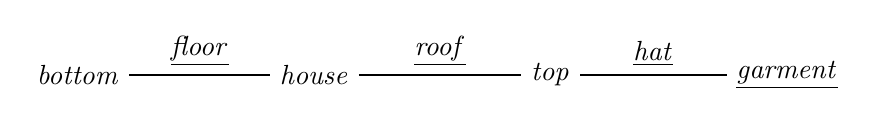
\begin{tikzpicture}
\node (1) at (0,0) {\cmubdata{bottom}};
\node (2) at (3,0) {\cmubdata{house}};
\node (3) at (6,0) {\cmubdata{top}};
\node (4) at (9,0) {{\underline{\cmubdata{garment}}}};
\draw (1) -- (2) node[anchor=south,inner sep=3pt,midway] {\underline{\cmubdata{floor}}};
\draw (2) -- (3) node[anchor=south,inner sep=3pt,midway] {\underline{\cmubdata{roof}}};
\draw (4) -- (3) node[anchor=south,inner sep=3pt,midway] {\underline{\cmubdata{hat}}};
\end{tikzpicture}
\caption{Partial graph of the English words.}
\label{fig:Lango-EN-partial}
\end{figure}
\end{description}

We need to notice, in this case, that the connection between the nodes was not done using arrows, but lines, since the order of the constituents is not relevant.

Comparing the two graphs (Figures \ref{fig:Lango-step2} and \ref{fig:Lango-EN-partial}), notice that the partial graph  contains a chain of four words (\texttr{garment} -- \texttr{top} -- \texttr{house} -- \texttr{bottom}), and one of the end-nodes is underlined (meaning it is given in the corpus). Looking at the complete graph of Lango words (\figref{fig:Lango-step2}), we know for sure that the partial graph of English words (\figref{fig:Lango-EN-partial}) cannot be part of the small subgraph, since it only has two nodes. In the big subgraph (the T-shaped one), only one node is underlined, namely \cmubdata{gìn}. Thus, we deduce that \wordtrans{gìn}{garment}, and the four nodes (\texttr{garment} -- \texttr{top} -- \texttr{house} -- \texttr{bottom}) can either be \cmubdata{gìn} -- \cmubdata{wìc} -- \cmubdata{ɔ̀t} -- \cmubdata{dyè}, or \cmubdata{gìn} -- \cmubdata{wìc} -- \cmubdata{ɔ̀t} -- \cmubdata{cɛ̀m}. Either way, the first three words are identical, so we deduce that \wordtrans{gìn}{garment}, \wordtrans{gìn wìc}{hat}, \wordtrans{wìc}{top}, \wordtrans{wìc ɔ̀t}{roof}, \wordtrans{ɔ̀t}{house}. Following this, the proposed graph becomes the one shown in \figref{fig:Lango-step3}.
\end{mysolution}

\begin{figure}[H]
%   \includegraphics[width=\linewidth]{images/Lango-step-3.png}
\vskip2\baselineskip
\begin{tikzpicture}
    \node (1) at (0,0) {{\cmubdata{dyè}}};
    \node (2) at (2.75,0) {\texttr{house}};
    \node (3) at (5.5,0) {\texttr{top}};
    \node (4) at (2.75,-2) {{\cmubdata{c\`{ɛ}m}}};
    \node (5) at (-2.75,0) {{\cmubdata{ty\`{ɛ}n}}};
    \node (6) at (8.25,0) {\texttr{\underline{garment}}};
    \node (7) at (5.5,-2) {{\underline{\cmubdata{ɲíg}}}};
    \node (8) at (8.25,-2) {{\cmubdata{wàŋ}}};
    \draw[-{Stealth[]}] (1) -- (2) node[anchor=south,inner sep=3pt,midway] {\underline{\phantom{~~~~~~~~~~~~}}};
    \draw[-{Stealth[]}] (3) -- (2) node[anchor=south,inner sep=3pt,midway] {\underline{\texttr{roof}}};
    \draw[-{Stealth[]}] (2) -- (4) node[anchor=south,inner sep=3pt,midway,right] {\underline{\phantom{~~~~~~~~~~~~}}};
    \draw[-{Stealth[]}] (1) -- (5) node[anchor=south,inner sep=3pt,midway] {\underline{\phantom{~~~~~~~~~~~~}}};
    \draw[-{Stealth[]}] (6) -- (3) node[anchor=south,inner sep=3pt,midway] {\underline{\texttr{hat}}};
    \draw[-{Stealth[]}] (7) -- (8) node[anchor=south,inner sep=3pt,midway] {\underline{\phantom{~~~~~~~~~~~~}}};
\end{tikzpicture}
\caption{Partially solved graph.}
\label{fig:Lango-step3}
\end{figure}


 Moreover, we know that one of the words \cmubdata{cɛ̀m} and \cmubdata{dyè} means \texttr{bottom}.

The remaining English words are: \texttr{floor} (which we know represents \texttr{house $+$ bottom}), \texttr{grain}, \texttr{eyeball}, \texttr{restaurant}, and \texttr{sole of foot}. We can already assume that \texttr{sole of foot} is connected to \texttr{bottom} (the bottom of the foot\slash leg\slash body). Thus, if \cmubdata{cɛ̀m} is \texttr{bottom}, we would not be able to connect it to \texttr{foot}, therefore \wordtrans{dyè}{bottom} and \wordtrans{tyɛ̀n}{foot}. We can now modify the graph (see \figref{fig:Lango-step4}).

\begin{figure}[H]
% % %   \includegraphics[width = \linewidth]{images/Lango-step4.png}
\vskip2\baselineskip
\begin{tikzpicture}
    \node (1) at (0,0)  {\texttr{bottom}};
    \node (2) at (2.75,0)  {\texttr{house}};
    \node (3) at (5.5,0)  {\texttr{top}};
    \node (4) at (2.75,-2) {{\cmubdata{c\`{ɛ}m}}};
    \node (5) at (-2.75,0) {\texttr{foot}};
    \node (6) at (8.25,0)  {\texttr{\underline{garment}}};
    \node (7) at (5.5,-2) {{\underline{\cmubdata{ɲíg}}}};
    \node (8) at (8.25,-2) {{\cmubdata{wàŋ}}};
    \draw[-{Stealth[]}] (1) -- (2) node[anchor=south,inner sep=3pt,midway] {\underline{\texttr{floor}}};
    \draw[-{Stealth[]}] (3) -- (2) node[anchor=south,inner sep=3pt,midway] {\underline{\texttr{roof}}};
    \draw[-{Stealth[]}] (2) -- (4) node[anchor=south,inner sep=3pt,midway,right] {\underline{\phantom{~~~~~~~~~~~~}}};
    \draw[-{Stealth[]}] (1) -- (5) node[anchor=south,inner sep=3pt,midway] {\underline{\texttr{sole}}};
    \draw[-{Stealth[]}] (6) -- (3) node[anchor=south,inner sep=3pt,midway] {\underline{\texttr{hat}}};
    \draw[-{Stealth[]}] (7) -- (8) node[anchor=south,inner sep=3pt,midway] {\underline{\phantom{~~~~~~~~~~~~}}};
\end{tikzpicture}
\caption{Partially solved graph, including \texttr{bottom} and \texttr{foot}.}
\label{fig:Lango-step4}
\end{figure}

 We are left with three words: \texttr{restaurant}, \texttr{eyeball}, and \texttr{grain}. Moreover, we know that one of them needs to be connected to \texttr{house} (\texttr{house} $+$ \cmubdata{cɛ̀m}), while the other two must be derived from one another (\cmubdata{ɲíg} and \cmubdata{ɲíg wàŋ}). Among the English words, the one which is most closely related semantically with \texttr{house} is \texttr{restaurant} (\texttr{restaurant} $=$ \texttr{house} $+$ \texttr{food}), while \texttr{eyeball} can be derived from \texttr{grain} as in \texttr{eyeball} $=$ \texttr{grain} $+$ \texttr{eye} (the grain of the eye).

Thus, we can make all the correspondences:
\begin{mysolution}
\begin{assgts}
    \item 
    \begin{tabular}[t]{lcll}
        \cmubdata{dyè ɔ̀t} & = &\texttr{floor} & (bottom + house) \\
        \cmubdata{dyè tyɛ̀n} & = &\texttr{sole of foot} & (bottom + foot) \\
        \cmubdata{gìn} & = &\texttr{garment} & \\
        \cmubdata{gìn wìc} & = &\texttr{hat} & (garment + top) \\
        \cmubdata{ɲíg} & = &\texttr{grain} &  \\
        \cmubdata{ɲíg wàŋ} & = &\texttr{eyeball} & (grain + eye) \\
        \cmubdata{ɔ̀t cɛ̀m} & = &\texttr{restaurant} & (house + food) \\
        \cmubdata{wìc ɔ̀t} & = &\texttr{roof} & (top + house) \\
    \end{tabular}
\item \begin{tabular}[t]{lcl} \cmubdata{cɛ̀m} & = & \texttr{food} \\
                               \cmubdata{dyè} & = & \texttr{bottom}\\
      \end{tabular}
\end{assgts}

 For task (c), we need to use the words we already have. Thus, we deduce that \texttr{window} $=$ eye of the house $=$ \texttr{eye} $+$ \texttr{house} (we deduce the word order from the phrase \texttr{eyeball} $=$ grain of the eye $=$ \texttr{grain} $+$ \texttr{eye}, and not *\texttr{eye} $+$ \texttr{grain}). Thus, \texttr{window} = \cmubdata{wàŋ ɔ̀t}.

This is, however, an easy problem for which a graph is not necessarily needed, since one can observe that the only word which occurs in three different phrases is \cmubdata{ɔ̀t}, and the only three English translations which have something in common are \texttr{floor}, \texttr{roof}, and \texttr{restaurant} (they are connected to a house\slash building). Nevertheless, the problem above offers an easy-to-understand example for the way in which graphs can be used to solve this type of problem.

We can now try to apply this method to solving a more complex problem.
\end{mysolution}

\pagebreak
\begin{problem}{\langnameGuarani}{\nameASouza}{\LOYear{\RoLOAbbr}{2021}}
\IntroWordComb{\langnameGuarani}\ \IntroAndEnglishRandom:

\begin{center}
    \begin{longtable}{rl@{\hskip0.5in}cl}
       \chaosline{jaxy}{water}
       \chaosline{jaxy-tata}{brave}
       \chaosline{jaxy endy}{thumb}
       \chaosline{kuã guaxu}{liver, heart}
       \chaosline{kuã regua}{fire}
       \chaosline{py'a}{smoke}
       \chaosline{py'a guaxu}{pregnant}
       \chaosline{tata}{ring (jewellery)}
       \chaosline{tata endy}{moonlight}
       \chaosline{tata rataxĩ}{firelight}
       \chaosline{ye guaxu}{moon}
       \chaosline{yvy rataxĩ}{good soil}
       \chaosline{yvy porã}{dust}
       \chaosline{yy}{star}
    \end{longtable}
\end{center}

\begin{assgts}
\item \detcorr
\item \transinen
\begin{multicols}{3}
\begin{enumerate}[start = 15]
    \item \cmubdata{guaxu}
    \item \cmubdata{porã} 
    \item \cmubdata{rataxĩ}
    \item \cmubdata{regua}
    \item \cmubdata{ye}
\end{enumerate}
\end{multicols}
\item \transinen[\langnameGuarani]
\begin{multicols}{3}
\begin{enumerate}[start = 20]
    \item \texttr{calm, relaxed}
    \item \texttr{fog}
    \blankitem
\end{enumerate}
\end{multicols}
\end{assgts}
\end{problem}

\begin{mysolution}


 First notice that in English we have words referring to organs (\texttr{liver, heart}) and emotions (\texttr{brave} and, in task (c), \texttr{calm}). So we can expect that these two are connected. Nevertheless, the first step is constructing the graphs for the Guaraní words (see \figref{fig:Guarani-step1}).

% \begin{figure}[ht]
%   \includegraphics[width = 0.8\linewidth]{images/Guarani-1.png}
% \end{figure}

\begin{figure}[H]
\caption{Complete graph of the words and phrases in Guaraní.}
\label{fig:Guarani-step1}
%   \includegraphics[width = \linewidth]{images/Lango-step4.png}
\begin{tikzpicture}
    \node (1) at (0,0) {\cmubdata{endy}};
    \node (2) at (2,0) {\uwave{\cmubdata{tata}}};
    \node (3) at (4,0) {\cmubdata{rataxĩ}};
    \node (4) at (6,0) {\cmubdata{yvy}};
    \node (5) at (8,0) {\cmubdata{porã}};
    \node (6) at (1,2) {\uwave{\cmubdata{jaxy}}};
    \draw[-{Stealth[]}] (2) -- (1) node[anchor=south,inner sep=3pt,midway] {\uwave{\phantom{~~~~~~}}};
    \draw[-{Stealth[]}] (2) -- (3) node[anchor=south,inner sep=3pt,midway] {\uwave{\phantom{~~~~~~}}};
    \draw[-{Stealth[]}] (4) -- (3) node[anchor=south,inner sep=3pt,midway] {\uwave{\phantom{~~~~~~}}};
    \draw[-{Stealth[]}] (5) -- (4) node[anchor=south,inner sep=3pt,midway] {\uwave{\phantom{~~~~~~}}};
    \draw[-{Stealth[]}] (6) -- (1) node[anchor=south,inner sep=3pt,midway,left] {\uwave{\phantom{~~~~~~}}};
    \draw[-{Stealth[]}] (6) -- (2) node[anchor=south,inner sep=3pt,midway,right] {\uwave{\phantom{~~~~~~}}};
\end{tikzpicture}
  
\begin{tikzpicture}
    \node (1) at (0,0) {\cmubdata{ye}};
    \node (2) at (2,0) {\cmubdata{guaxu}};
    \node (3) at (4,0) {\cmubdata{kuã}};
    \node (4) at (6,0) {\cmubdata{regua}};
    \node (5) at (3,-1.5) {\uwave{\cmubdata{yy}}};
    \node (6) at (2,2) {\uwave{\cmubdata{py'a}}};
    \draw[-{Stealth[]}] (1) -- (2) node[anchor=south,inner sep=3pt,midway] {\uwave{\phantom{~~~~~~}}};
    \draw[-{Stealth[]}] (3) -- (2) node[anchor=south,inner sep=3pt,midway] {\uwave{\phantom{~~~~~~}}};
    \draw[-{Stealth[]}] (3) -- (4) node[anchor=south,inner sep=3pt,midway] {\uwave{\phantom{~~~~~~}}};
    \draw[-{Stealth[]}] (6) -- (2) node[anchor=south,inner sep=3pt,midway,right] {\uwave{\phantom{~~~~~~}}};
\end{tikzpicture}
\end{figure}


\note{In Appendix~\ref{appendix:3} I present a hand-drawn graph in order to show what such a graph might look like in reality, when solving a problem.}


We notice that, in Guaraní, we have three independent subgraphs. For the partial graph of English words, we have the words: \texttr{moon}, \texttr{fire}, \texttr{moonlight}, and \texttr{firelight}. These can be arranged in a graph as shown in \figref{fig:Guarani-step2}.

% \begin{figure}[ht]
%   \caption{}

% \end{figure}

\begin{figure}[H]
% \includegraphics[width = 0.4\linewidth]{images/Guarani-2.png}
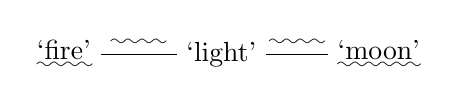
\begin{tikzpicture}
\node (1) at (2,0) {\uwave{\texttr{fire}}};
\node (2) at (4,0) {\texttr{light}};
\node (3) at (6,0) {\uwave{\texttr{moon}}};
\draw (1) -- (2) node[anchor=south,inner sep=3pt,midway] {\uwave{{~~~~~~}}};
\draw (2) -- (3) node[anchor=south,inner sep=3pt,midway] {\uwave{{~~~~~~}}};
\end{tikzpicture}
\caption{Partial graph of the English words \texttr{moon}, \texttr{fire}, \texttr{moonlight}, and \texttr{firelight}.}
\label{fig:Guarani-step2}
\end{figure}



 This is an ideal partial graph since we have two base words (nodes), \texttr{fire}, and \texttr{moon}, which are found in the corpus and are both connected to the same word (\texttr{light}). According to the Guaraní graph in \figref{fig:Guarani-step1}, the only two nodes close to one another that are found in the corpus (are underlined) are \cmubdata{jaxy} and \cmubdata{tata}, and both of them are connected to the word \cmubdata{endy}. Thus, we deduce that \wordtrans{endy}{light}, and \{\cmubdata{jaxy}, \cmubdata{tata}\} = \{\texttr{fire}, \texttr{moon}\}\footnote{By this notation, we mean that \cmubdata{jaxy} and \cmubdata{tata} correspond to \texttr{fire} and \texttr{moon}, but we do not know which is which.}. In order to determine which is which, we notice that \cmubdata{jaxy} is not connected to anything else, while \cmubdata{tata} is further connected to \cmubdata{rataxĩ}. In English, we have the word \texttr{smoke} which is clearly connected to \texttr{fire}, so \wordtrans{tata}{fire} and \wordtrans{jaxy}{moon}. Moreover, from the graph, we notice that \cmubdata{jaxy} and \cmubdata{tata} combine with one another, thus, in English, we need to find a word formed by combining the words \texttr{moon} and \texttr{fire}. The only one which is semantically close to that is \texttr{star} ( = \texttr{fire moon}). Adding this information, our graph will look like that in \figref{fig:Guarani-step3}.

\begin{figure}
  \caption{Partially solved graph.}
\label{fig:Guarani-step3}
% %   \includegraphics[width = \linewidth]{images/Guarani-3.png}
  \begin{tikzpicture}[every node/.style={align=center}]
    \node (1) at (0,0) {\cmubdata{endy}\\(\texttr{light})};
    \node (2) at (3,0) {\uwave{\cmubdata{tata}}\\(\texttr{fire})};
    \node (3) at (6,0) {\cmubdata{rataxĩ}};
    \node (4) at (8,0) {\cmubdata{yvy}};
    \node (5) at (10,0) {\cmubdata{porã}};
    \node (6) at (1.5,2) {\uwave{\cmubdata{jaxy}}\\ (\texttr{moon})};
    \draw[-{Stealth[]}] (2) -- (1) node[anchor=south,inner sep=3pt,midway] {\uwave{\texttr{firelight}}};
    \draw[-{Stealth[]}] (2) -- (3) node[anchor=south,inner sep=3pt,midway] {\uwave{\texttr{smoke}}};
    \draw[-{Stealth[]}] (4) -- (3) node[anchor=south,inner sep=3pt,midway] {\uwave{\phantom{~~~~~~}}};
    \draw[-{Stealth[]}] (5) -- (4) node[anchor=south,inner sep=3pt,midway] {\uwave{\phantom{~~~~~~}}};
    \draw[-{Stealth[]}] (6) -- (1) node[anchor=south,inner sep=3pt,midway,left] {\uwave{\texttr{moonlight}}};
    \draw[-{Stealth[]}] (6) -- (2) node[anchor=south,inner sep=3pt,midway,right] {\uwave{\texttr{star}}};
\end{tikzpicture}\bigskip\\  
\begin{tikzpicture}[every node/.style={align=center}]
  \node (1) at (0,0) {\cmubdata{ye}};
  \node (2) at (3,0) {\cmubdata{guaxu}};
  \node (3) at (6,0) {\cmubdata{kuã}};
  \node (4) at (9,0) {\cmubdata{regua}};
  \node (5) at (4.5,-1.5) {\uwave{\cmubdata{yy}}};
  \node (6) at (3,2) {\uwave{\cmubdata{py'a}}};
  \draw[-{Stealth[]}] (1) -- (2) node[anchor=south,inner sep=3pt,midway] {\uwave{\phantom{~~~~~~}}};
  \draw[-{Stealth[]}] (3) -- (2) node[anchor=south,inner sep=3pt,midway] {\uwave{\phantom{~~~~~~}}};
  \draw[-{Stealth[]}] (3) -- (4) node[anchor=south,inner sep=3pt,midway] {\uwave{\phantom{~~~~~~}}};
  \draw[-{Stealth[]}] (6) -- (2) node[anchor=south,inner sep=3pt,midway,right] {\uwave{\phantom{~~~~~~}}};
\end{tikzpicture}
\end{figure}


 As mentioned above, \texttr{fire} is only combined with one more word and, in English, the only word that belongs to the same semantic field is \texttr{smoke}. Thus, \wordtrans{tata rataxĩ}{smoke}. Nevertheless, we cannot immediately deduce the meaning of \cmubdata{rataxĩ} (\texttr{smoke} = \texttr{fire} $+$ $X$). However, looking at the English words, we notice the word \texttr{dust} and, since this roughly relates to the same semantic area as \texttr{smoke}, they most likely have something in common (the word $X$). Thus, we get:

\begin{exe}
 \sn[]{\texttr{smoke} = \texttr{fire} $+$ $X$ \quad\quad\quad\quad and \quad\quad\quad\quad \texttr{dust} = ? $+$ $X$}
\end{exe}

Comparing again the remaining words, we notice we have the phrase \texttr{good soil} (and, indeed, \texttr{smoke} is to \texttr{fire} as \texttr{dust} is to \texttr{soil}). Therefore, $X$ represents \texttr{particles/powder} (smoke is a ``powder'' from the fire, while dust is a powder of soil). Thus, we can complete the top subgraph as shown in \figref{fig:Guarani-step4}.

\begin{figure}
% % %   \includegraphics[width = 0.9\linewidth]{images/Guarani-4.png}
\caption{Completely solved top subgraph.}
\label{fig:Guarani-step4}
\begin{tikzpicture}[every node/.style={align=center}]
    \node (1) at (0,0) {\cmubdata{endy}\\ (\texttr{light})};
    \node (2) at (3,0) {\uwave{\cmubdata{tata}} \\ (\texttr{fire})};
    \node (3) at (6,0) {\cmubdata{rataxĩ}\\ (\texttr{powder}/\\ \texttr{particles})};
    \node (4) at (8,0) {\cmubdata{yvy}\\ (\texttr{soil})};
    \node (5) at (10,0) {\cmubdata{porã}\\ (\texttr{good})};
    \node (6) at (1.5,2) {\uwave{\cmubdata{jaxy}}\\ (\texttr{moon})};
    \draw[-{Stealth[]}] (2) -- (1) node[anchor=south,inner sep=3pt,midway] {\uwave{\texttr{firelight}}};
    \draw[-{Stealth[]}] (2) -- (3) node[anchor=south,inner sep=3pt,midway] {\uwave{\texttr{smoke}}};
    \draw[-{Stealth[]}] (4) -- (3) node[anchor=south,inner sep=3pt,midway] {\uwave{\texttr{dust}}};
    \draw[-{Stealth[]}] (5) -- (4) node[anchor=south,inner sep=3pt,midway] {\texttr{good\\ \uwave{soil}}};
    \draw[-{Stealth[]}] (6) -- (1) node[anchor=south,inner sep=3pt,midway,left] {\uwave{\texttr{moonlight}}};
    \draw[-{Stealth[]}] (6) -- (2) node[anchor=south,inner sep=3pt,midway,right] {\uwave{\texttr{star}}};
\end{tikzpicture}
\end{figure}

Since this subgraph is independent (not connected to the others in any way), we have reached a dead end and we need to build a new partial graph based on the English words. However, we have already made eight correspondences. The remaining words are:

\begin{center}
\begin{tabular}{rl@{\hskip0.5in}cl}
      4. & \cmubdata{kuã guaxu} & A. & \texttr{water} \\
      5. & \cmubdata{kuã regua} & B. & \texttr{brave} \\
      6. & \cmubdata{py'a} & C. & \texttr{thumb} \\
      7. & \cmubdata{py'a guaxu} & D. & \texttr{liver, heart} \\
      11. & \cmubdata{ye guaxu} & G. & \texttr{pregnant} \\
      14. & \cmubdata{yy} & H. & \texttr{ring} \\
\end{tabular}
\end{center}


Among these, we can notice \texttr{ring} and \texttr{thumb} (both being related to the word \texttr{finger}, as in \texttr{thumb} = \texttr{finger} + \texttr{big} and \texttr{ring} = \texttr{finger} + \texttr{jewellery/ornament}). Only based on these two words, we can build the graph shown in \figref{fig:Guarani-step5}.

\begin{figure}[H]
%   \includegraphics[width =.5\linewidth]{images/Guarani-5.png}
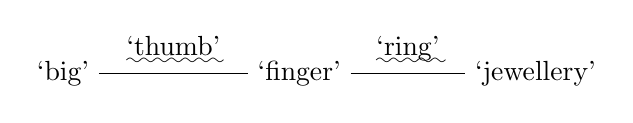
\begin{tikzpicture}[every node/.style={align=center}]
    \node (1) at (2,0) {{\texttr{big}}};
    \node (2) at (5,0) {\texttr{finger}};
    \node (3) at (8,0) {{\texttr{jewellery}}};
    \draw (1) -- (2) node[anchor=south,inner sep=3pt,midway] {\uwave{\texttr{thumb}}};
    \draw (2) -- (3) node[anchor=south,inner sep=3pt,midway] {\uwave{\texttr{ring}}};
\end{tikzpicture}
\caption{Partial graph.}
\label{fig:Guarani-step5}
\end{figure}

 Thus, \texttr{finger} can correspond to either \cmubdata{kuã}, or \cmubdata{guaxu}. If it corresponded to \cmubdata{guaxu}, it needs to combine with another word among those given (i.e., \texttr{finger} $+$ \texttr{water}, \texttr{finger} $+$ \texttr{brave}, \texttr{finger} $+$ \texttr{liver, heart}, \texttr{finger} $+$ \texttr{pregnant}), all of these combinations being highly unlikely (difficult to justify). Therefore, \wordtrans{kuã}{finger}. Moreover, we notice that no other word seems to belong in the semantic field of the word \texttr{jewellery, ornament}, so, most likely this is the meaning of \cmubdata{regua}. The graph now looks like that shown in \figref{fig:Guarani-step6}.
 
\begin{figure}
%   \includegraphics[width = 0.7\linewidth]{images/Guarani-6.png}
\caption{Completely solved subgraph.}
\label{fig:Guarani-step6}
\begin{tikzpicture}[every node/.style={align=center}]
    \node (1) at (0,0) {\cmubdata{ye}};
    \node (2) at (3,0) {\cmubdata{guaxu}\\ (\texttr{big})};
    \node (3) at (6,0) {\cmubdata{kuã}\\(\texttr{finger})};
    \node (4) at (10,0) {\cmubdata{regua}\\(\texttr{jewellery})};
    \node (5) at (3,2) {\uwave{\cmubdata{py'a}}};
    \draw[-{Stealth[]}] (1) -- (2) node[anchor=south,inner sep=3pt,midway] {\uwave{\phantom{~~~~~~}}};
    \draw[-{Stealth[]}] (3) -- (2) node[anchor=south,inner sep=3pt,midway] {\uwave{\texttr{thumb}}};
    \draw[-{Stealth[]}] (3) -- (4) node[anchor=south,inner sep=3pt,midway] {\uwave{\texttr{ring}}};
    \draw[-{Stealth[]}] (5) -- (2) node[anchor=south,inner sep=3pt,midway,right] {\uwave{\phantom{~~~~~~}}};
\end{tikzpicture}
\end{figure}

We need to have in the corpus two more words which are formed from the combination of \texttr{big} with other words (and one of the words it combines with -- \cmubdata{py'a} -- must also appear in the corpus). The first word we notice is \texttr{pregnant} (we can consider that it is formed as \texttr{belly} $+$ \texttr{big} or something similar). Moreover, we notice that we have \texttr{liver, heart} and \texttr{brave} among the remaining words. As mentioned above, words for emotions are often formed from words designating organs, so \texttr{brave} = \texttr{big} $+$ \texttr{heart, liver} is quite plausible. In this way, we also completed this subgraph and the only remaining word, \cmubdata{yy}, must mean \texttr{water}.

So we have the correspondences:


\begin{center}
    \begin{tabular}{rlcll}
         1. & \cmubdata{jaxy} & = & \texttr{moon} &  \\
         2. & \cmubdata{jaxy-tata} & = & \texttr{star} & (moon + fire) \\
         3. & \cmubdata{jaxy endy} & = & \texttr{moonlight} &  \\
         4. & \cmubdata{kuã guaxu} & = & \texttr{thumb} & (finger + big) \\
         5. & \cmubdata{kuã regua} & = & \texttr{ring} & (finger + jewellery) \\
         6. & \cmubdata{py'a} & = & \texttr{liver, heart} &  \\
         7. & \cmubdata{py'a guaxu} & = & \texttr{brave} & (liver, heart + big) \\
         8. & \cmubdata{tata} & = & \texttr{fire} &  \\
         9. & \cmubdata{tata endy} & = & \texttr{firelight} &  \\
         10. & \cmubdata{tata rataxĩ} & = & \texttr{smoke} & (fire + powder) \\
         11. & \cmubdata{ye guaxu} & = & \texttr{pregnant} & (belly + big) \\
         12. & \cmubdata{yvy rataxĩ} & = & \texttr{dust} & (soil + powder) \\
         13. & \cmubdata{yvy porã} & = & \texttr{good soil} & (soil + good)  \\
         14. & \cmubdata{yy} & = & \texttr{water} &  \\
    \end{tabular}
\end{center}


In task (b), we are only asked to translate simple words (which correspond to the nodes of the graph), so this task is straightforward now: \wordtrans{guaxu}{big}, \wordtrans{porã}{good}, \wordtrans{rataxĩ}{powder}, \wordtrans{regua}{ornament/jewellery}, \wordtrans{ye}{belly}.

\remember{For this type of problem, there might be multiple acceptable answers, which is taken into account when grading. Thus, for the word \cmubdata{regua} (which must be deduced from the combination \texttr{ring} = \texttr{finger} $+$ \cmubdata{regua}), there can be multiple interpretations: \texttr{ornament}, \texttr{jewellery} etc., but it can also be considered to mean \texttr{circle}, \texttr{surrounding}, etc. (which is the actual meaning of the Guaraní word). Thus, all of these words would be equally acceptable.}

 In task (c), we are asked to translate the words \texttr{fog} and \texttr{calm}. The word \texttr{fog} is easy to translate since it resembles \texttr{dust} and \texttr{smoke} (thus, \texttr{fog} = \texttr{water} $+$ \texttr{powder}), so its translation is \cmubdata{yy rataxĩ}. The word \texttr{calm} can be compared with the word \texttr{brave} (both referring to human qualities). Since \texttr{brave} was formed from \texttr{liver, heart}, it is likely that \texttr{calm} is too. Moreover, we notice that we also have another adjective: \texttr{good}. Therefore, we can form the combination \texttr{calm} = \texttr{good} + \texttr{liver, heart}. Thus, its translation is \cmubdata{py'a porã}.



Put all together, the answers are:

\begin{assgts}
    \item
    \begin{enumerate}
    \begin{multicols}{7}
        \item K.
        \item N.
        \item I.
        \item C.
        \item H.
        \item D.
        \item B.
        \item E.
        \item J.
        \item F.
        \item G.
        \item M.
        \item L.
        \item A.
        \end{multicols}
    \end{enumerate}
    \item
    \begin{enumerate}[start = 15]
    \begin{multicols}{2}
        \item \texttr{big}
        \item \texttr{good}
        \item \texttr{powder, particles}
        \item \texttr{circle}
        \item \texttr{belly, stomach}
        \item[] \hphantom{x}
        \end{multicols}
    \end{enumerate}

    \item
    \begin{enumerate}[start = 20]
    \begin{multicols}{2}
        \item \cmubdata{py'a porã}
        \item \cmubdata{yy rataxĩ}
        \end{multicols}
    \end{enumerate}
\end{assgts}
\end{mysolution}


\hypertarget{practice-problems}{%
\section{Practice problems}}

\begin{problem}{\langnameBasque}{\nameNZaika}{\LOYear{\MSKAbbr}{2012}}
\IntroWords{\langnameBasque}\ \IntroAndEnglishRandom:

\begin{exe}
\sn[]{\cmubdata{igogailu}, \cmubdata{artzain}, \cmubdata{lantegi}, \cmubdata{lantalde}, \cmubdata{bizitegi}, \cmubdata{taldekide}, \cmubdata{erizain}, \cmubdata{garbigailu}, \cmubdata{ikastalde}, 
      \cmubdata{bizikide}, \cmubdata{garbitegi}, \cmubdata{ikaskide}, \cmubdata{lankide}, \cmubdata{eritegi}, \cmubdata{artalde}
\glt \texttr{classmate}, \texttr{flatmate}, \texttr{flock of sheep}, \texttr{crew}, \texttr{elevator}, \texttr{clinic}, \texttr{factory}, \texttr{nurse}, \texttr{home}, \texttr{shepherd},         
     \texttr{wash-house}, \texttr{colleague}, \texttr{washing machine}, \texttr{team member}, \texttr{class (of students)}}
\end{exe}

\begin{assgts}
\item \detcorr
\item How is the word \cmubdata{artalde} different from the other Basque words?
\item Translate the word \texttr{sheep-pen} into Basque, knowing that it has the same feature as the word \cmubdata{artalde}.
\end{assgts}
\end{problem}



\begin{problem}{\langnameTurkish}{\nameMChoudhury}{\LOYear{\PLOAbbr}{2014}}
\IntroWords{\langnameTurkish}\ \IntroAndEnglishRandom:

\begin{exe}\sloppy
\sn[]{\cmubdata{gözlemci}, \cmubdata{döndürmek}, \cmubdata{gündöndü}, \cmubdata{gözlükcü}, \cmubdata{şarkıcı}, \cmubdata{çocukluk}, \cmubdata{gözlemek}, \cmubdata{pazar}, \cmubdata{pazartesi}, \cmubdata{cumartesi}, \cmubdata{güneşli}
\glt \texttr{Saturday}, \texttr{Sunday}, \texttr{Monday}, \texttr{observer}, \texttr{singer}, \texttr{to observe}, \texttr{to rotate}, \texttr{sunny}, \texttr{sunflower}, \texttr{optician}, \texttr{childhood}}
\end{exe}

\begin{assgts}
\item \detcorr
\item \transinen[\langnameTurkish]
\begin{enumerate}
    \item \texttr{observation}
    \item \texttr{child}
    \item \texttr{the state of being a singer}
    \item \texttr{spectacles}
    \item \texttr{Friday}
    \blankitem
\end{enumerate}
\end{assgts}
\end{problem}

\begin{problem}{\langnameChinese}{\nameRDinca}{\LOYear{\RoLOAbbr}{2015}}
\IntroWordComb{\langnameChinese}\ \IntroAndEnglishRandom:

\begin{exe}
\sn[]{\cmubdata{hóng}, \cmubdata{míngbái}, \cmubdata{báishì}, \cmubdata{huáng}, \cmubdata{hēishì}, \cmubdata{shìqing huángle}, \cmubdata{yăn}, \cmubdata{yănhóng}, \cmubdata{hóngshì}, \cmubdata{hóngyán}, \cmubdata{hēihuà}, \cmubdata{báiyăn}, \cmubdata{báihuà}, \cmubdata{hēibái fēnmíng}, \cmubdata{yán}, \cmubdata{hēibái}, \cmubdata{huángle}
\glt \texttr{encoding}, \texttr{black-and-white}, \texttr{face}, \texttr{yellow}, \texttr{funeral}, \texttr{bankruptcy}, \texttr{to clarify}, \texttr{to dislike}, \texttr{young woman}, \texttr{failure}, \texttr{decoding}, \texttr{wedding}, \texttr{eye}, \texttr{black market}, \texttr{it's written in black and white}, \texttr{jealousy}, \texttr{red}}
\end{exe}

\begin{assgts}
\item \detcorr
\item The word \cmubdata{báishì} can have two meanings in Chinese, although only one is reflected in the correspondences above. What is the other meaning? 
\end{assgts}
\end{problem}



\begin{problem}{\langnameHausa}{\namePHelmer}{\LOYear{\RoLOAbbr}{2019}}
\IntroPhrases{\langnameHausa}\ \IntroAndEnglishRandom:

\begin{table}[H]
    \begin{tabular}{rl@{\hskip0.5in}cl}
       \chaosline{bàakín rúwáa}{talkative boy}
       \chaosline{bàbbán bàakín tsúntsúu}{white camel}
       \chaosline{bàbbán yátsàa}{big beak}
       \chaosline{bàbbán ràkúmín rúwáa}{thumb}
       \chaosline{bàbbán yár sháanúu}{fruit}
       \chaosline{bákín cíkìi}{fork}
       \chaosline{bákín ràagóo}{pregnant woman}
       \chaosline{cóokàlíi mài yátsàa}{sorrow}
       \chaosline{dán ràagóo}{estuary}
       \chaosline{dán mài bàbbán bàakíi}{lamb}
       \chaosline{fárin ràkúmíi}{black sheep}
       \chaosline{rúwán bíshíyàa}{(tree) sap}
       \chaosline{yár mài bàbbán cíkìi}{tsunami}
       \chaosline{yár bíshíyàa}{big heifer}
    \end{tabular}
\end{table}

\begin{assgts}
\item \detcorr
\item \transinen
\begin{multicols}{2}
\begin{enumerate}[start = 15]
    \item \cmubdata{dán sháanúu}
    \item \cmubdata{fárín cíkìi} 
    \item \cmubdata{yár mài bákin bàakíi} 
\end{enumerate}
\end{multicols}
\item \transinen[\langnameHausa]
\begin{multicols}{2}
\begin{enumerate}[start = 18]
    \item \texttr{girl who has a spoon}
    \item \texttr{crow}
    \item \texttr{river}
    \item \texttr{(tree) branch}

\end{enumerate}
\end{multicols}

\end{assgts}

\begin{tblsWarning}
An \texttr{estuary} is a wide part of the river, similar to a funnel. A \texttr{heifer} is a young female cow. 
\end{tblsWarning}
\end{problem}



\begin{problem}{\langnameTetum}{\nameAPegusevs}{\LOYear{\RoLOAbbr}{2020}}
\IntroWordComb{\langnameTetum}\ \IntroAndEnglishRandom:

\begin{table}[H]
    \begin{tabular}{rl@{\hskip0.5in}cl}
       \chaosline{ai boot}{eyelid}
       \chaosline{ai fuan boot}{scapula}
       \chaosline{ai fuan musan}{leaf}
       \chaosline{ai tahan}{big fruit}
       \chaosline{ibun kulit boot}{big tree}
       \chaosline{kbas}{auricle}
       \chaosline{kbas tahan}{skin}
       \chaosline{kulit}{seed}
       \chaosline{matan kulit}{shoulder}
       \chaosline{matan musan}{eyeball}
       \chaosline{tilun tahan}{big lip}
    \end{tabular}
\end{table}

\begin{assgts}
\item \detcorr
\pagebreak
\item \transinen
\begin{multicols}{3}
\begin{enumerate}[start = 12]
    \item \cmubdata{matan fuan}
    \item \cmubdata{ai fuan kulit} 
    \item \cmubdata{tilun boot} 
\end{enumerate}
\end{multicols}
\item[] One of the phrases has the same translation as one of the phrases 1--11.
\item \transinen[\langnameTetum]
\begin{multicols}{2}
\begin{enumerate}[start = 15]
    \item \texttr{mouth}
    \item \texttr{big eye}
    \item \texttr{(tree) bark}
    \item \texttr{grain}
\end{enumerate}
\end{multicols}
\item Two of the words above can be combined to construct a phrase meaning \texttr{impolite person}. Which ones are these? 
\end{assgts}

\begin{tblsWarning}
The \texttr{scapula} (or shoulder blade) is the large flat bone that is part of the shoulder joint. The \texttr{auricle} is the visible part of the ear. 
\end{tblsWarning}
\end{problem}



\begin{problem}{\langnameMalagasy}{\nameAKretov}{\LOYear{\MSKAbbr}{2011}}
\IntroWordComb{\langnameMalagasy}\ \IntroAndEnglishRandom:
\begin{center}
    \begin{tabular}{r@{~~}l@{\hskip1em}c@{~~}l}
       \chaosline{mahandohalika}{grandson}
       \chaosline{lohalika}{ankle}
       \chaosline{zafin-kitrokely}{shoot of rice (departing from the stem)}
       \chaosline{hafaladia}{up to the sole}
       \chaosline{zafim-bary}{rice field}
       \chaosline{kitrokely}{great-great-great-grandson}
       \chaosline{zafim-paladia}{one who can get on his knees}
       \chaosline{zafy}{great-great-great-great--grandson}
       \chaosline{tanim-bary}{knee}
       \chaosline{mahambozona}{one who can carry something on his neck}
    \end{tabular}
\end{center}

\begin{assgts}
\item \detcorr
\pagebreak
\item \transinen
\begin{multicols}{3}
\begin{enumerate}[start = 11]
    \item \cmubdata{tany}
    \item \cmubdata{vozona}
    \item \cmubdata{halohalika} 
\end{enumerate}
\end{multicols}
\item \transinen[\langnameMalagasy]
\begin{multicols}{2}
\begin{enumerate}[start = 14]
    \item \texttr{great-great-grandson}
    \item \texttr{sole}
    \item \texttr{up to the ankle}
\end{enumerate}
\end{multicols}
\end{assgts}

\begin{tblsWarning}
\cmubdata{y} = \texttr{i} in \texttr{pit}.
\end{tblsWarning}
\end{problem}



\hypertarget{solutions-of-practice-problems}{%
\section{Solutions of practice problems}}

\begin{practiceproblemsolution}{8.3. \langnameBasque}

\begin{solutions}[label=Solution 8.3\alph*]
    \item
    \begin{itemize}
        \item[] \wordtrans{igogailu}{elevator}
        \item[] \wordtrans{artzain}{shepherd}
        \item[] \wordtrans{lantegi}{factory}
        \item[] \wordtrans{lantalde}{crew}
        \item[] \wordtrans{bizitegi}{home}
        \item[] \wordtrans{taldekide}{team member}
        \item[] \wordtrans{erizain}{nurse}
        \item[] \wordtrans{garbigailu}{washing machine}
        \item[] \wordtrans{ikastalde}{class of (students)}
        \item[] \wordtrans{bizikide}{flatmate}
        \item[] \wordtrans{garbitegi}{wash-house}
        \item[] \wordtrans{ikaskide}{classmate}
        \item[] \wordtrans{lankide}{colleague}
        \item[] \wordtrans{eritegi}{clinic}
        \item[] \wordtrans{artalde}{flock of sheep}
    \end{itemize}
    \item \cmubdata{-t $+$ t- \rightarrow\ -t-} (if a morpheme which ends in \cmubdata{t} is joined to another that starts with \cmubdata{t}, one of the two \cmubdata{t}'s is dropped).
    \item \texttr{sheep-pen} = \cmubdata{artegi}
\end{solutions}

\rules

 Each Basque word is composed of two morphemes (the first one shows the semantic field, while the other the category):

\begin{table}[H]
\begin{tabular}{ll}
\lsptoprule
     1\textsuperscript{st} morpheme & 2\textsuperscript{nd} morpheme \\
\midrule
     \wordtrans{igo-}{to lift} &  \\
     \wordtrans{lan-}{to work} & \wordtrans{-zain}{worker}\footnote{In reality, a more accurate translation would be \texttr{keeper}.} \\
     \wordtrans{bizi-}{to live} & \wordtrans{-tegi}{place} \\
     \wordtrans{art-}{sheep} & \wordtrans{-talde}{collective} \\
     \wordtrans{eri-}{sick} & \wordtrans{-kide}{member} \\
     \wordtrans{garbi-}{to wash} & \wordtrans{-gailu}{machine} \\
     \wordtrans{ikas-}{to learn} &  \\
 \lspbottomrule
\end{tabular}
\end{table}

\end{practiceproblemsolution}
 \begin{practiceproblemsolution}{8.4. \langnameTurkish}

 \begin{solutions}[label=Solution 8.4\alph*]
     \item The morphemes have been separated by a hyphen (-) and their meaning is given, in order, between brackets:
     \noindent
     \begin{center}
         \begin{tabular}{@{}l @{~} l @{~} l@{}}
             \cmubdata{göz-lem-ci}  &  \texttr{observer} & (eye + abstract-noun + agent-marker) \\
             \cmubdata{göz-lük-cü}  &  \texttr{optician} & (eye + state-of-being + agent-marker) \\
             \cmubdata{göz-le(m)-mek}  &  \texttr{to observe} & (eye + abstract-noun + verb-marker) \\
             \cmubdata{döndür-mek}  &  \texttr{to rotate} & (rotation + verb-marker) \\
             \cmubdata{gün(eş)-li}  &  \texttr{sunny} & (sun + adjective-marker) \\
             \cmubdata{gün-döndü}  &  \texttr{sunflower} & (sun + rotation) \\
             \cmubdata{şarkı-cı}  &  \texttr{singer} & (song + agent-marker) \\
             \cmubdata{çocuk-luk}  &  \texttr{childhood} & (child + state-of-being) \\
             \cmubdata{pazar}  &  \texttr{Sunday} &  \\
             \cmubdata{pazar-tesi}  &  \texttr{Monday} & (Sunday + tomorrow) \\
             \cmubdata{cumar-tesi}  &  \texttr{Saturday} & (Friday + tomorrow) \\
         \end{tabular}
     \end{center}
     
    \note{Since Turkish is a language displaying vowel harmony, the form of the suffixes will differ depending on the word (\cmubdata{ci/cı/cü} or \cmubdata{lük/luk}).}
  \item
     \begin{enumerate}
         \item \cmubdata{gözlem}
         \item \cmubdata{çocuk}
         \item \cmubdata{şarikcilik}
         \item \cmubdata{gözlük}
         \item \cmubdata{cumar}\footnote{In reality, it is \cmubdata{cuma}, but \cmubdata{cumar} is the answer as can be deduced from the given data.}
     \end{enumerate}
 \end{solutions}
 \end{practiceproblemsolution}

 \begin{practiceproblemsolution}{8.5. \langnameChinese}

 \begin{solutions}[label=Solution 8.5\alph*]
 \item
     \begin{itemize}[leftmargin=0pt]
     \begin{multicols}{2}
         \item[] \wordtrans{hóng}{red}
         \item[] \wordtrans{míngbái}{to clarify}
         \item[] \wordtrans{báishì}{funeral}
         \item[] \wordtrans{huáng}{yellow}
         \item[] \wordtrans{hēishì}{black market}
         \item[] \wordtrans{shìqing huángle}{bankruptcy}
         \item[] \wordtrans{y\v{a}n}{eye}
         \item[] \wordtrans{y\v{a}nhóng}{jealousy}
         \item[] \wordtrans{hóngshì}{wedding}
         \item[] \wordtrans{hóngyán}{young woman}
         \item[] \wordtrans{hēihuà}{encoding}
         \item[] \wordtrans{báiy\v{a}n}{to dislike}
         \item[] \wordtrans{báihuà}{decoding}
         \item[] \wordtrans{hēibái fēnmíng}{it is written in black and white}
         \item[] \wordtrans{yán}{face}
         \item[] \wordtrans{hēibái}{black-and-white}
         \item[] \wordtrans{huángle}{failure}
         \end{multicols}
     \end{itemize}
     \item \texttr{white market}
 \end{solutions}
 \end{practiceproblemsolution}

\pagebreak
\begin{practiceproblemsolution}{8.6. \langnameHausa}

 \begin{solutions}[label=Solution 8.6\alph*]
     \item
     \begin{enumerate}
     \begin{multicols}{7}
        \item I.
        \item C.
        \item D.
        \item M.
        \item N.
        \item H.
        \item K.
        \item F.
        \item J.
        \item A.
        \item B.
        \item L.
        \item G.
        \item E.
     \end{multicols}
     \end{enumerate}
     \item 15. \texttr{calf} (boy + cow)
     \item[] 16. \texttr{happiness} (white + stomach) -- based on \texttr{sorrow} = black + stomach
     \item[] 17. \texttr{impolite/naughty girl} (girl + with + black + mouth)
     \item 18. \cmubdata{yár mài cóokàlíi} (girl + with + spoon)
     \item[] 19. \cmubdata{bákín tsúntsúu} (bird + black)
     \item[] 20. \cmubdata{bàbbán rúwáa} (big + water)
     \item[] 21. \cmubdata{yátsàn bíshíyàa} (finger + tree)
 \end{solutions}

 \rules 
 \begin{itemize}
 \item The determiners come before the head noun;
 \item The words \wordtrans{yár}{female, woman} and \wordtrans{mài}{with} are invariable;
 \item All other words end in \cmubdata{-n} if they are not the head noun or they double the final vowel if they are the head noun. An alternative explanation is that they end in \cmubdata{-n}, unless they are phrase-final, in which case the \cmubdata{-n} is removed and the last vowel is doubled.


\end{itemize}
 \end{practiceproblemsolution}

\begin{practiceproblemsolution}{8.7. \langnameTetum}

\begin{solutions}[label=Solution 8.7\alph*]
     \item
     \begin{enumerate}
     \begin{multicols}{6}
        \item E.
        \item D.
        \item H.
        \item C.
        \item K.
        \item I.
        \item B.
        \item G.
        \item A.
        \item J.
        \item F.
        \item[] \quad
     \end{multicols}
     \end{enumerate}
     \item
     \begin{enumerate}[start = 12]
     \begin{multicols}{3}
        \item \texttr{eyeball}
        \item \texttr{(fruit) peel}
        \item \texttr{big ear}
     \end{multicols}
     \end{enumerate}
     \item
     \begin{enumerate}[start = 15]
     \begin{multicols}{3}
        \item \cmubdata{ibun}
        \item \cmubdata{matan boot}
        \item \cmubdata{ai kulit}
        \item \cmubdata{musan}
     \end{multicols}
     \end{enumerate}
     \item \cmubdata{ibun boot} (\texttr{big mouth})
     \end{solutions}
\end{practiceproblemsolution}


     \begin{practiceproblemsolution}{8.8. \langnameMalagasy}

     \begin{solutions}[label=Solution 8.8\alph*]
         \item
     \begin{enumerate}
     \begin{multicols}{5}
        \item G.
        \item I.
        \item F.
        \item D.
        \item C.
        \item B.
        \item H.
        \item A.
        \item E.
        \item J.
     \end{multicols}
     \end{enumerate}
     \item
     \begin{enumerate}[start = 11]
     \begin{multicols}{3}
        \item \texttr{field}
        \item \texttr{neck}
        \item \texttr{up to the knee}
     \end{multicols}
     \end{enumerate}
     \item
     \begin{enumerate}[start = 14]
     \begin{multicols}{3}
        \item \cmubdata{zafin-dohalika}
        \item \cmubdata{faladia}
        \item \cmubdata{hakitrokely}
     \end{multicols}
     \end{enumerate}
     \end{solutions}
     \end{practiceproblemsolution}

\section*{Explanations}

When two words combine (A--B), there are some phonological changes occurring in both of them. Thus, the first word (the prefix) undergoes some alternations at the end. If it ends in \cmubdata{y}, it will become \cmubdata{iN} (where \cmubdata{N} is a nasal which assimilates to the place of articulation of the next consonant -- \cmubdata{m} for \cmubdata{p/b} and \cmubdata{n} for \cmubdata{d/k}) -- e.g., \cmubdata{zafi\textbf{n}-\textbf{k}itrokely} and \cmubdata{zafi\textbf{m}-\textbf{p}aladia}.

The following word ($B$) undergoes an initial consonant mutation, depending on whether the prefix ends in a vowel or a consonant, as follows:

\begin{table}[H]
    \begin{tabular}{ccc}
    \lsptoprule
        First consonant of $B$ & after vowel & after consonant \\\midrule
        \cmubdata{l} & \cmubdata{l} & \cmubdata{d}\\
        \cmubdata{v} & & \cmubdata{b}\\
        \cmubdata{k} & & \cmubdata{k}\\
        (?) & \cmubdata{f} & \cmubdata{p}\\
    \lspbottomrule 
    \end{tabular}
\end{table}


Since we are asked to find (?) (in task c), the only rule we can deduce is that there is no initial consonant mutation if the word before ends in a vowel.

\begin{sloppypar}
Interestingly, the words for \texttr{great-grandson}, \texttr{great-great-grandson}, etc. are based on vertical position of body parts: the more distant the descendant, the lower the position of the body part used. The terms \texttr{great-great-grandson}, \texttr{great-great-great-grandson}, and \texttr{great-great-great-great-grandson} are formed by compounding \wordtrans{zafy}{grandson} with \texttr{knee}, \texttr{ankle}, and \texttr{sole}, respectively.
\end{sloppypar}


% \section{Further reading}
% \begin{enumerate}[{label=[\arabic{*}]}]
%     \item ten Hacken, Pius (ed.). “The semantics of compounding.”\ \textit{Cambridge University Press}, Cambridge (2016).
%     \item Koptjevskaja-Tamm, Maria and Liljegren, Henrik. “Semantic patterns from an areal perspective.”\ in “The Cambridge handbook of areal linguistics.”\ \textit{Cambridge University Press}, Cambridge (2017).
%     \item Kroeger, Paul. “Analyzing meaning: an introduction to semantics and pragmatics.”\ \textit{Language Science Press}, Berlin (2022).
%     \item Vanhove, Martine (ed.). “From polysemy to semantic change.”\ \textit{John Benjamins Publishing Company}, Amsterdam (2008).
% \end{enumerate}
\nocite{tenHacken2016, KoptjevskajaTammLiljegren2017, Kroeger2022, Vanhove2008}
% \printbibliography[heading=FurtherReading]
\FurtherReadingBox{}

\end{refsection}

\begin{refsection}
\hypertarget{numbers}{%
\chapter{Number systems}\label{chap-numbers}}

\hypertarget{introduction}{%
\section{Introduction}}

 In order to understand problems about number systems, we firstly need to understand the concept of base and the characteristics of such systems.

In Romanian, for example, the number 432 is written \cmubdata{patru sute treizeci și doi}. It can be segmented into morphemes as follows: \cmubdata{patru} (\texttr{four}) \cmubdata{sute} (\texttr{hundreds}) \cmubdata{trei} (\texttr{three})-\cmubdata{zeci} (\texttr{tens}) \cmubdata{și} (\texttr{and}) \cmubdata{doi} (\texttr{two}), and each morpheme has a well defined role. The morphemes \cmubdata{patru}  (\texttr{four}), \cmubdata{trei} (\texttr{three}), \cmubdata{doi} (\texttr{two}) represent the \textit{digits}, the basic units, while the morphemes \cmubdata{sute} (\texttr{hundreds}) and \cmubdata{zeci} (\texttr{tens}) represent the \textit{orders}, i.e., some greater base words. Finally, the morpheme \cmubdata{și} (\texttr{and}) denotes addition. Since in this case the orders are 10 and 100 (10\textsuperscript{1}, 10\textsuperscript{2}), we are talking about a base-10 (or decimal) system.

Moreover, word order plays an important role, together with the way in which the multiplication and the addition are marked. Returning to the example \cmubdata{patru sute treizeci și doi}, we can deduce the following:

\begin{itemize}
    \item the general order is from big to small (we first write the hundreds, then the tens and finally the units);
    \item the multiplier is placed before the order (thus, we write \cmubdata{patru sute} and not \cmubdata{*sute patru});
    \item the morpheme for \texttr{tens} is written as part of the same word with its multiplier (\cmubdata{treizeci}, not \cmubdata{*trei zeci});
    \item the tens are separated from the units by the word \cmubdata{și}.
\end{itemize}

 There is also a simpler method to show all of these rules, by writing the general structure of the number:

\exrule{100X + 10Y + Z = X \cmubdata{sute} Y-\cmubdata{zeci și} Z}

 This rule combines all four rules from above, showing the sequence of the orders (hundreds, tens, units), the position of the multiplier (as a separate word before the hundreds and combined with the ending \cmubdata{zeci} for tens), as well as the morpheme \cmubdata{și} added between tens and units.

Although base 10 is the most common base and most languages use it, there are also other bases, among which the most common are base 6 and base 20. Less common, but occurring in a reasonable number of languages are bases 4, 5, 12, and 60, while bases 7, 9, 11, and 13 are extremely rare (at the moment, no known natural language uses them), so that, in linguistics problems, we can assume from the beginning that the system is highly unlikely to have the bases 7, 9, 11, 13.

A special category of bases is 22–28, which are found in languages whose number system is based on body parts, such as Oksapmin or Kaugel.

In order to better understand the concept of base, let us consider how the numbers 10, 25, and 100 would be written in a base-6 system. Since the base is 6, the orders are 6 (6\textsuperscript{1}), 36 (6\textsuperscript{2}), 216 (6\textsuperscript{3}), and so on. Therefore, the number 10 will be written as $6+4$ (or $4+6$, depending on the word order), number 25 will be written as $(4\times6)+1$, while 100 will be written as $(2\times36)+(4\times6)+4$.

So, in problems involving number systems, there are two important characteristics:

\begin{enumerate}[label = (\arabic*)]
    \item word order (or direction): big-to-small or small-to-big or a mixture;
    \item the way in which addition and multiplication are marked (or whether they are not overtly marked).
\end{enumerate}

In terms of (1), remember that it is not necessary that the word order is strictly ascending or descending, and there can also be exceptions. For example, in German, 432 is written \cmubdata{vierhundertzweiunddreißig} (\cmubdata{vier-hundert-zwei-und-drei-ßig} = 4-\texttr{hundreds}-2-\texttr{plus}-3-\texttr{tens}), so the order is hundreds-units-tens. In terms of (2), note that in French, for example, in the number 2,510 (\cmubdata{deux mille cinq cent dix} = \texttr{two} - \texttr{thousand} - \texttr{five} - \texttr{hundred} - \texttr{ten}), both the addition and the multiplication are implicit and as such, if the digit is placed before the order, it gets multiplied, while addition occurs every time after the order (e.g., 2,510 can be written as $(2\times1000)+(5\times100)+10$). Moreover, if the addition or multiplication is marked, this will be done using a rather pervasive morpheme, word, or group of words.

\begin{problem}{\langnameQuenya}{\nameRDinca}{\LOYear{\RoLOAbbr}{2013}}
Here are some Quenya numbers:
\begin{center}
    \begin{tabular}{lr@{\qquad\qquad}lr}
         \pbsvnum{neldë}{3} & \pbsvnum{enquë yucainen}{26} \\
         \pbsvnum{canta}{4} & \pbsvnum{minë nelcainen}{31} \\
         \pbsvnum{lempë}{5} & \pbsvnum{cancainen}{40} \\
         \pbsvnum{otso}{7} & \pbsvnum{atta tolcainen}{82} \\
         \pbsvnum{tolto}{8} & \pbsvnum{atta tolcainen tuxa}{182} \\
         \pbsvnum{nelcëa}{13} & \pbsvnum{nertë nelcainen lemtuxa}{539} \\
         \pbsvnum{encëa}{16} & \pbsvnum{}{} \\
    \end{tabular}
\end{center}

\begin{assgts}
\item \taskWriteNumbers:
\begin{multicols}{2}
\begin{enumerate}[label = \alph*.]
    \item \cmubdata{tolcëa}
    \item \cmubdata{enquë cancainen}
    \item \cmubdata{cancainen neltuxa}
    \item \cmubdata{lempë tolcainen}
    \item \cmubdata{tuxa}
    \blankitem
\end{enumerate}
\end{multicols}
\item \taskWriteIn{\langnameQuenya}: 1, 70, 192, 385.
\end{assgts}
\end{problem}

\begin{mysolution}

 We notice that numbers 13 and 16 both end in the suffix \cmubdata{-cëa}, while numbers bigger than 26 have a different structure. Thus, comparing the words for 3 and 13, we can assume it is a base-10 language and that numbers $10$ $+$ $X$ are written as \cmubdata{X-cëa}. We further notice that in order to form the number 13, only a part of the word for 3 is used (\cmubdata{nel}).

Comparing examples 82 and 182, they differ only by the word \cmubdata{tuxa} placed at the end; therefore, we can deduce that \cmubdata{tuxa} means 100 (which further confirms that the number system for this language is base 10). Moreover, looking at the number 539, we notice that the last word is \cmubdata{lemtuxa}, where \cmubdata{tuxa} = 100, and \cmubdata{lem} is the first part of the number 5. Thus, in this case as well, only a part of the stem of the unit is used. Furthermore, we notice that in the right column, the second word always ends in \cmubdata{cainen}. We can assume that this is the suffix which marks the tens ($10X$), whence we deduce that the word order in Quenya is units-tens-hundreds.

Only based on these observations, we can write the following rules:

\exrule{$10+X$ = $X$′ \cmubdata{-cëa} \quad\quad\quad $100X+10Y+Z$ = $Z$ $Y$′\cmubdata{-cainen} $X$′\cmubdata{-tuxa}}

 By $X$′ and $Y$′ we mean that a different, truncated, form of the word is used.

 Based on these observations, we can create a table with the form of each digit in different contexts:

\begin{table}[H]
    \begin{tabular}{clccc}
    \lsptoprule
    Digit & \multicolumn{1}{c}{$X$} & $10+X$ & $10X$ & $100X$ \\\midrule
    1 & \cmubdata{minë} & & & $\varnothing$ \\
    2 & \cmubdata{atta} & &\cmubdata{yu-} & \\
    3 & \cmubdata{neldë} & \cmubdata{nel-} & \cmubdata{nel-} & \\
    4 & \cmubdata{canta} & & \cmubdata{can-}& \\
    5 & \cmubdata{lempë} & & & \cmubdata{lem-} \\
    6 & \cmubdata{enquë} & \cmubdata{en-} & & \\
    7 & \cmubdata{otso} & & & \\
    8 & \cmubdata{tolto} & & \cmubdata{tol-} & \\
    9 & \cmubdata{nertë} & & & \\
    \lspbottomrule
    \end{tabular}
\end{table}

The four columns represent the form in which the respective digit is used if it represents the units, if it appears with the suffix \cmubdata{-cëa} (meaning $10+X$), if it appears with the suffix \cmubdata{-cainen} ($10X$), or if it appears with the suffix \cmubdata{-tuxa} ($100X$).

We notice that the same form of 3 appears both in the case of $10+X$ and $10X$. Therefore, we deduce that both contexts use the same form. Moreover, we have no reason not to assume that the same form will also be used in the case of hundreds. In order to deduce how that form is constructed, we compare it with the full form in the first column (the units). We notice that the short form (which we designated by $X$′ and $Y$′) represents the first syllable of the unit. The only exception is the digit 2, where the form used for 20 is \cmubdata{yu-}. It appears that in Quenya 1 and 2 are irregular and have different forms in different contexts. This is not uncommon cross-linguistically. 

Thus, we can solve the tasks and write the rules.

\rules Digits are single words. In compound words, only the stem of the digit is used, which is represented by the first syllable (in the notation below, $X$′ is the stem/first syllable of $X$). The digit 2 has a special form, \cmubdata{yu-}. Thus:

\exrule{$10+X$ = $X$′\cmubdata{-cëa} \quad\quad\quad $100X+10Y+Z$ = $Z$ $Y$′\cmubdata{-cainen} $X$′\cmubdata{-tuxa}}

\pagebreak
\begin{assgts}
    \item
     \begin{multicols}{5}
        \begin{enumerate}[leftmargin = 1em, label = \alph*.]
            \item 18
            \item 46
            \item 340
            \item 85
            \item 100
        \end{enumerate}
    \end{multicols}
    \item
    \begin{multicols}{2}
    \setlength\columnsep{2em}
        \begin{itemize}[leftmargin = 0em]
            \item[] 1 = \cmubdata{minë}
            \item[] 70 = \cmubdata{otcainen}
            \item[] 192 = \cmubdata{atta nercainen tuxa}
            \item[] 385 = \cmubdata{lempë tolcainen neltuxa}
        \end{itemize}
    \end{multicols}
\end{assgts}

 In situations where the base is unknown, a simple method to get some additional information is to count how many morphemes there are. If in a particular language we count 11 digits, we expect the base to be, most likely, 10 or 12. Usually, this method is just an estimation, and the result should probably be taken with an error margin of ±2 because: (1) it is possible that we misidentified some of the digits, and (2) it is possible that the problem does not feature all the digits or even some digits might have different forms in different contexts. Moreover, it is extremely important that we count only the digits, not other morphemes (such as orders or addition/multiplication markers).

\end{mysolution}
\begin{problem}{\langnameChami}{\nameVNeacsu}{\LOYear{\PLOAbbr}{2022}}
Here are two equalities in Embera Chami:
\begin{center}
\begin{tabular}{@{}cr@{\hskip0.02in}c@{\hskip0.02in}l@{}}
     \eqline{umbea $+$ huasoma kwimane}{omme huasoma omme}
     \eqline{omme huasoma kwimane $+$ huasoma abba}{kwimane huasoma}
\end{tabular}
\end{center}

\begin{assgts}
\item Write the equalities above with numerals.
\item \taskWriteIn{\langnameChami}: 1, 5, 17, 23.
\end{assgts}
\end{problem}

\begin{mysolution}

At first sight, it might seem a very difficult problem without an obvious starting point and with very little information given. Nevertheless, if we check the structure of the numbers, we notice that there are two types: single words or numbers like $X$ \cmubdata{huasoma} $Y$. We can assume that the second type will represent bigger numbers, and that \cmubdata{huasoma} is the base, these numbers representing $X\times \text{\cmubdata{huasoma}} + Y$ (or $Y × \text{\cmubdata{huasoma}} + X$). Moreover, we notice that the same word can represent both $X$ and $Y$, therefore $X$ and $Y$ are the slots where the digits are placed. Based on these rules, we can try to count the number of digits that occur in the problem, and we notice that there are only four (\cmubdata{umbea}, \cmubdata{kwimane}, \cmubdata{omme}, \cmubdata{abba}). Moreover, they have a constant form (there are no changes or added or deleted morphemes). We can then assume that the base is 5 and that \cmubdata{huasoma} = 5.

The next thing we need to do is figure out the order of the constituents, i.e., figure out whether $X$ \cmubdata{huasoma} $Y$ means $5X + Y$ or $5Y + X$. Looking at equality (1), we have two cases:


\begin{enumerate}[label = \alph*.]
\begin{multicols}{2}
    \item \cmubdata{huasoma} $X = 5X$
    \item \cmubdata{huasoma} $X = 5+X$
    \end{multicols}
\end{enumerate}


 Assuming case a. is true, eq. (1) becomes:

\exrule{$\text{\cmubdata{umbea}}+5\times\text{\cmubdata{kwimane}} = \text{\cmubdata{omme}}+5\times\text{\cmubdata{omme}}$}

 This seems unlikely, since we know that \cmubdata{umbea} is, most likely, a digit. Thus, if \cmubdata{huasoma kwimane} meant $5X$, then \cmubdata{umbea} $+$ \cmubdata{huasoma kwimane} should be equal to \cmubdata{umbea huasoma kwimane} (i.e., \cmubdata{umbea} $+ 5\times$\cmubdata{kwimane}). Generally, the carryover\footnote{We use the term \textit{carryover} for the following situation: when you add 17 and 19, you add the units first (7 and 9 to get 16) and “carry over”\ the 1 (from 16) to the tens.} is a strong strategy to discover certain digits.

Thus, case b. must be correct, and now we know that \cmubdata{huasoma} $X = 5 + X$, so we can deduce that $X$ \cmubdata{huasoma} $= 5X$ and, extrapolating, $X$ \cmubdata{huasoma} $Y = 5X + Y$.

Moreover, from eq. (1), we see that the number resulting from the addition has the multiplier \cmubdata{omme}. Since this is the result of a sum between a unit and a number like base $+$ $X$, the result can either also be base $+$ $X$ (if there is no carryover) or $2\times$base $+$ $X$ (if there is carryover). Since we know that there is carryover (the number on the right has a multiplier, since it has the structure $5X+Y$), we deduce that \cmubdata{omme} = 2.

If we denote the remaining three digits by $U$, $K$ and $A$ (corresponding to their first letter), we can rewrite the equalities as follows:
\begin{enumerate}[leftmargin = 5em, label = (\arabic*)]
    \item $U+(5+K)=12$
    \item $(10+K)+(5+A)=5K$
\end{enumerate}

 Rearranging equality (1), we get: $U + K = 7$.

Knowing that $U$ and $K$ are digits smaller than $5$ (the base), $U$ and $K$ can only correspond to $3$ and $4$, not necessarily in this order. Thus, $A$ can only be $1$ since it is the only remaining digit. Therefore, \cmubdata{abba} $= 1$.

Replacing this in eq. (2) gives us: $10 + K + 6 = 5K \Leftrightarrow 4K = 16$. So $K = 4$ and, subsequently, $U = 3$.

Thus, the rules are:
\begin{itemize}
    \item 1 = \cmubdata{abba}, 2 = \cmubdata{omme}, 3 = \cmubdata{umbea}, 4 = \cmubdata{kwimane}, 5 = \cmubdata{huasoma};
    \item $5X + Y = X$ \cmubdata{huasoma} $Y$.
\end{itemize}

\begin{solutions}
    \item
    \begin{multicols}{2}
        \begin{enumerate}[label = (\arabic*)]
            \item $3+9=12$
            \item $14+6=20$
        \end{enumerate}
    \end{multicols}
    \item
    \begin{itemize}
        \item[] $1 =$ \cmubdata{abba}
        \item[] $5 =$ \cmubdata{huasoma}
        \item[] $17 = 3\times5+2 =$ \cmubdata{umbea huasoma omme}
        \item[] $23 = 4\times5+3 =$ \cmubdata{kwimane huasoma umbea}
    \end{itemize}
\end{solutions}
\end{mysolution}

\begin{discussion}
For this problem, notice that counting the digits and understanding the structure of the numbers is extremely important for number problems. Moreover, carryovers offer valuable information for problems in which equalities are given, and they can usually be used to infer the digits 2 and 3.

Moreover, it is important to mention that, in order to be able to solve the problem, we need to use the fact that the problem is self-sufficient, otherwise we cannot deduce that the base is 5. Let us consider a base $B$ and the following values for the digits: \cmubdata{omme} $= 2$, \cmubdata{kwimane} $= 4$, \cmubdata{abba} $= B-4$, \cmubdata{umbea} $= B-2$. The equalities become:

\begin{enumerate}[leftmargin = 5em, label = (\arabic*)]
    \item $(B–2) + B + 4 = 2B + 2$
    \item $2B + 4 + (B + (B–4)) = 4B$
\end{enumerate}

 In this case, the two equalities hold, no matter the base (e.g., for base 13 we would get the equalities: (1) $11 + 17 = 28$ and (2) $30 + 22 = 52$). Nevertheless, task (b) asks for the translation of 1, so \cmubdata{abba} needs to be 1 (we know that \cmubdata{umbea} is bigger than \cmubdata{abba}, since $B-4 < B-2$), and if \cmubdata{abba} $= 1 = B-4 \Rightarrow B = 5$.

This is the complete thought process based upon which we deduce the base is 5. However, generally, we expect that the problem features all (or almost all) digits, enabling us to estimate the base based on counting the digits.
\end{discussion}

\begin{problem}{\langnameYupik}{\nameKLow}{\LOYear{\UKLOAbbr}{2017}}
Yup'ik people have an interesting concept when it comes to counting – the words for the numbers can be broken down into meaningful parts which may be related to body parts. For example, the word for 5, \cmubdata{talliman}, means \texttr{arm} and the word for 6, \cmubdata{arvinlegen}, means \texttr{cross over}, as you need to change hands to go on counting. 

The Yup'ik people often include geometry in the border patterns of their traditional garments, called "parkas". One such pattern comes from a $3\times3$ square, as represented below. This is a magic square, constructed by placing the digits 1 to 9 within the cells such that the sum of all the digits in every row, column, and diagonal is the same.
\begin{center}
\includegraphics[width = 4cm]{images/Yupik_square.jpg}
\end{center}

To help you fill in the magic square, the following clues are given in Yup'ik.
\textit{Hint:} 294 in Yup'ik is \cmubdata{yuinaat qula cetaman qula cetaman}.

\begin{itemize}
\item Rows:
    \begin{enumerate}[label = \alph*.,nosep]
     \item \cmubdata{Yuinaat yuinaq cetaman qula malruk}
     \item \cmubdata{Yuinaat akimiaq malruk akimiaq malruk}
     \item \cmubdata{Yuinaat yuinaak malruk akimiaq atauciq}
     \end{enumerate}
\item Columns:
    \begin{enumerate}[nosep]
      \item \cmubdata{Yuinaat yuinaq atauciq akimiaq pingayun}
      \item \cmubdata{Yuinaat yuinaak malruk yuinaat malrunglegen qula atauciq}
      \item \cmubdata{Yuinaat qula pingayun akimiaq atauciq}
    \end{enumerate}
\end{itemize}


\begin{assgts}
\item Fill in the numbers missing from the magic square above. One digit is already given (a2 = 9).
\item Write in Yup'ik the number given in the diagonal from top left (the number formed by the digits a1-b2-c3).

\end{assgts}
\end{problem}

\begin{mysolution}

\subsubsection*{1. Solving the magic square}

This is in reality the easiest part. It is known that in a magic square the middle number must be 5 (you can attempt a mathematical proof, it is rather easy), hence b2 = 5. Moreover, it is known that the sum on every row, column and diagonal must be 15. Since on the middle column we already have 9 and 5, we deduce that c2 = 1.

On the first row, we already have the digit 9, so the sum of the other two digits must be 6. We have three possibilities: 5 and 1 (impossible, since 5 is already used), 3 and 3 (impossible, since we cannot repeat digits), or 4 and 2 (this is therefore the only possible option). Therefore, the first row can be either 492 or 294. Since in the introduction we are given the Yup'ik name for 294, which does not appear in the crossword clues (hence, it doesn't appear in the square), we deduce that the first row must be 492, so a1 = 4, a3 = 2.

Since we are told that the sum on the diagonals is also constant (so, 15), we can easily deduce that c1 = 8 and c3 = 6, which makes filling in the rest of the square trivial. In the end we get:

\begin{center}
\includegraphics[width = 4cm]{images/Yupik_Square-solved.png}
\end{center}

\subsubsection*{2. Solving the number problem}

 Once the square is filled in, we can extract all the information in a table, transforming the problem into a classic one, in which we are given some numbers spelled out in Yup'ik:

    \begin{longtable}{cl}
    276 & \cmubdata{yuinaat qula pingayun akimiaq atauciq} \\
    294 & \cmubdata{yuinaat qula cetaman qula cetaman} \\
    357 & \cmubdata{yuinaat akimiaq malruk akimiaq malruk} \\
    438 & \cmubdata{yuinaat yuinaq atauciq akimiaq pingayun} \\
    492 & \cmubdata{yuinaat yuinaq cetaman qula malruk} \\
    816 & \cmubdata{yuinaat yuinaak malruk akimiaq atauciq} \\
    951 & \cmubdata{yuinaat yuinaak malruk yuinaat malrunglegen qula atauciq} \\
    \end{longtable}

 The first important observation is based on the last word in every number. We have four types of numbers: ending in \cmubdata{atauciq} (276, 816, 951), ending in \cmubdata{malruk} (357, 492), ending in \cmubdata{cetaman} (294), and ending in \cmubdata{pingayun} (438). Looking closely, one notices that these numbers can be grouped based on their remainder when divided by 5 (i.e., modulo 5). Thus, we can deduce that:

\exrule{\cmubdata{atauciq} = 1, \cmubdata{malruk} = 2, \cmubdata{pingayun} = 3, \cmubdata{cetaman} = 4}

 Replacing these numbers, we get:

\exrule{
    \begin{tabular}{cl}
    276 & \cmubdata{yuinaat qula 3 akimiaq 1} \\
    294 & \cmubdata{yuinaat qula 4 qula 4} \\
    357 & \cmubdata{yuinaat akimiaq 2 akimiaq 2} \\
    438 & \cmubdata{yuinaat yuinaq 1 akimiaq 3} \\
    492 & \cmubdata{yuinaat yuinaq 4 qula 2} \\
    816 & \cmubdata{yuinaat yuinaak 2 akimiaq 1} \\
    951 & \cmubdata{yuinaat yuinaak 2 yuinaat malrunglegen qula 1} \\
    \end{tabular}
    }

 Since we assumed that the last number is added, we can simply subtract it (from the number representation) and delete it (from the spelled-out numbers). We are left with:

\exrule{
    \begin{tabular}{cl}
    275 & \cmubdata{yuinaat qula 3 akimiaq} \\
    290 & \cmubdata{yuinaat qula 4 qula} \\
    355 & \cmubdata{yuinaat akimiaq 2 akimiaq} \\
    435 & \cmubdata{yuinaat yuinaq 1 akimiaq} \\
    490 & \cmubdata{yuinaat yuinaq 4 qula} \\
    815 & \cmubdata{yuinaat yuinaak 2 akimiaq} \\
    950 & \cmubdata{yuinaat yuinaak 2 yuinaat malrunglegen qula} \\
    
    \end{tabular}
}

 Now we can easily notice that the numbers that end in 5 have the last word \cmubdata{akimiaq}, while those ending in 0 have the last word \cmubdata{qula}. Moreover, in the introduction we are told that 5 = \cmubdata{talliman}, so \cmubdata{akimiaq} cannot be 5 as well. We can therefore assume that \cmubdata{akimiaq} = 15, and \cmubdata{qula} = 10. Subtracting these numbers, we are left with:

\exrule{
    \begin{tabular}{cl}
    260 & \cmubdata{yuinaat 10 3} \\
    280 & \cmubdata{yuinaat 10 4} \\
    340 & \cmubdata{yuinaat 15 2} \\
    420 & \cmubdata{yuinaat yuinaq 1 3} \\
    480 & \cmubdata{yuinaat yuinaq 4} \\
    800 & \cmubdata{yuinaat yuinaak 2} \\
    940 & \cmubdata{yuinaat yuinaak 2 yuinaat malrunglegen} \\
    
    \end{tabular}
}

 Comparing the numbers 260 and 280, we notice that they differ only by 3 vs. 4, while their numerical difference is 20. Thus, we can deduce that \cmubdata{yuinaat} is 20 and it represents a multiplier. Therefore, 280 is written as \texttr{20\times} \texttr{10} \texttr{4}. Since $280 = 20\times14$, we deduce that the two numbers after \texttr{20\times} are firstly added together and then multiplied by 20. This is, \cmubdata{yuinaat} $X$ $Y = 20(X+Y)$.

Looking at 800, we notice it contains \cmubdata{yuinaak}, instead of \cmubdata{yuinaq}. Since we already know that \cmubdata{yuinaat} = \texttr{20\times}, replacing it we obtain: 800 = \texttr{20\times} \cmubdata{yuinaak} \texttr{2}. So \cmubdata{yuinaak} also means \texttr{20\times} (basically, it shows that the following number also needs to be multiplied instead of added).
Therefore, 940 is written as \texttr{20\times 20\times\ 2 20\times\ } \cmubdata{malrunglegen}, from which we deduce that \cmubdata{malrunglegen} = 7, i.e., $940 = (20\times20\times2)+(20\times7)$.

Based on these, we can write all the rules and solve the tasks.

\begin{solutions}
\item \raisebox{-\height+\ht\strutbox}{\includegraphics[width = 4cm]{images/Yupik_Square-solved.png}}
     
\item $456 = 20\times (20+2)+15+1 =$ \cmubdata{yuinaat yuinaq malruk akimiaq atauciq}
\end{solutions}

\rules Numbers are written in base 20. Numbers smaller than 20 are written as $10 + A$ or $15 + A$ (where $A$ is 1, 2, 3, or 4). Numbers smaller than 400, i.e., $20A + B$, are written as \cmubdata{yuinaat} $A$ $B$, where $A$ and $B$ are between 1 and 19.

\pagebreak
Base words are:
\begin{enumerate}[leftmargin = 5em, label = \arabic*]

    \begin{multicols}{2}
    \item \cmubdata{atauciq}
    \item \cmubdata{malruk}
    \item \cmubdata{pingayun}
    \item \cmubdata{cetaman}
    \item \cmubdata{talliman} (given in intro)
    \item \cmubdata{arvinlegen} (given in intro)
    \item \cmubdata{malrunglegen}
    \item[10] \cmubdata{qula}
    \item[15] \cmubdata{akimiaq}
    \item[20] \cmubdata{yuinaq} (\texttr{20+}), \cmubdata{yuinaat} (\texttr{20\times})
        \end{multicols}
\end{enumerate}

\noindent Addition is implicit and the constituent order is from big to small. For numbers bigger than 800, a new structure is added at the beginning -- \cmubdata{yuinaat yuinaak} $X$, meaning $400X$, and the rest is written as above. For example, $951 = 800 + 151 = (20\times20\times2) + (20\times7) + 11 =$ \texttr{(20\times) (20\times) (2) (20\times) (7) (10) (1)} = \cmubdata{yuinaat yuinaak malruk yuinaat malrunglegen qula atauciq}.
\end{mysolution}

\section{Overcounting}

\begin{problem}{\langnameUmbuUngu}{\nameKGilyarova}{\LOYear{\IOLAbbr}{2012}}
\hfill
\begin{tabular}[t]{cl}
    \lsptoprule
      & \langnameUmbuUngu \\\midrule              
    10 & \cmubdata{rureponga talu}    \\ 
    15 & \cmubdata{malapunga yepoko}  \\ 
    20 & \cmubdata{supu}              \\ 
    21 & \cmubdata{tokapunga telu}    \\ 
    27 & \cmubdata{alapunga yepoko}   \\ 
    30 & \cmubdata{polangipunga talu} \\ 
    \lspbottomrule
\end{tabular}\hfill
\begin{tabular}[t]{cl}
        \lsptoprule
        &   \langnameUmbuUngu\\\midrule
     35 & \cmubdata{tokapu rureponga yepoko} \\
     40 & \cmubdata{tokapu malapu} \\ 
     48& \cmubdata{tokapu talu} \\ 
     50& \cmubdata{tokapu alapunga talu} \\ 
     69& \cmubdata{tokapu talu tokapunga telu} \\ 
     79& \cmubdata{tokapu talu polangipunga yepoko} \\ 
     97& \cmubdata{tokapu yepoko alapunga telu} \\ 
     \lspbottomrule
\end{tabular}\hfill\hbox{}

\begin{tblsWarning}
    \cmubdata{telu < yepoko}
\end{tblsWarning}

\pagebreak
\begin{assgts}
\item \taskWriteNumbers:
\begin{enumerate}[label = \alph*.]
    \item \cmubdata{tokapu polanigpu}
    \item \cmubdata{tokapu talu rureponga telu}
    \item \cmubdata{tokapu yepoko malapunga talu}
    \item \cmubdata{tokapu yepoko polangipunga telu}
\end{enumerate}
\item \taskWriteIn{\langnameUmbuUngu}: 13, 66, 72, 76, 95.
\end{assgts}
\end{problem}

\begin{mysolution}
Initial observations:
\begin{itemize}
    \item \cmubdata{supu} is a single word, so most likely is a multiple of the base; therefore the base can be 4, 5, 10, or 20;
    \item 10 is not a single word, so it is unlikely that the base is 5, 10 or 20. Therefore, it seems to be a base-4 language;
    \item \cmubdata{tokapu} occurs in the number 35 (but it does not occur in 30), so it most likely means 32. 31, 33 and 34 do not seem to make sense as single words, since they are extremely unlikely as bases, and it can't be 35 either since there are other words following it. Moreover, 32 confirms the hypothesis that the language is base-4, since it is a multiple of 4;
    \item General structure: (\cmubdata{tokapu}) ($X$) ($Y$\cmubdata{-pu(nga)}) ($Z$).
\end{itemize}

 Based on this structure, we can count the digits. These appear as $X$ or $Z$ (but we notice that they do not occur as $Y$, which means that $Y$\cmubdata{-pu(nga)} is a single word). There are only three words appearing in $X$ and $Z$ positions: \cmubdata{talu}, \cmubdata{telu}, \cmubdata{yepoko}.

Moreover, we notice that 48 is \cmubdata{tokapu talu}. Most likely, \cmubdata{talu} is a multiplier for \cmubdata{tokapu}, and, since the numbers smaller than 48 do not contain this structure, we deduce that \cmubdata{talu} = 2. Indeed, for numbers 35 and 40, \cmubdata{tokapu} occurs without a multiplier (1 is implicit), so the first multiplier that ought to appear is 2. Based on the same logic, \cmubdata{yepoko} must mean 3 and, knowing that \cmubdata{telu} $<$ \cmubdata{yepoko}, we get that \cmubdata{telu} is 1.

Replacing these numbers in the given data, we get:

\begin{center}
\hfill
\begin{tabular}[t]{cl}
\lsptoprule
       & \langnameUmbuUngu                \\\midrule
    10 & \cmubdata{rureponga} 2   \\
    15 & \cmubdata{malapunga} 3   \\
    20 & \cmubdata{supu}          \\
    21 & \cmubdata{tokapunga} 1   \\
    27 & \cmubdata{alapunga} 3    \\
    30 & \cmubdata{polangipunga} 2\\
\lspbottomrule
\end{tabular}\hfill
\begin{tabular}[t]{cl}
\lsptoprule
   & \langnameUmbuUngu \\  \midrule
35 & \cmubdata{tokapu rureponga} 3 \\
40 & \cmubdata{tokapu malapu} \\
48 & \cmubdata{tokapu} 2 \\
50 & \cmubdata{tokapu alapunga} 2 \\
69 & \cmubdata{tokapu} 2\cmubdata{tokapunga} 1 \\
79 & \cmubdata{tokapu} 2 \cmubdata{polangipunga} 3 \\
97 & \cmubdata{tokapu} 3 \cmubdata{alapunga} 1 \\
\lspbottomrule
\end{tabular}
\hfill\hbox{}
\end{center}

 Based on the number 48, since we assumed that 2 is a multiplier, we deduce that \cmubdata{tokapu} = 24. Moreover, based on the first column, by subtraction, we obtain the numbers: \cmubdata{rureponga} = 8, \cmubdata{malapunga} = 12, \cmubdata{supu} = 20, \cmubdata{tokapunga} = 20, \cmubdata{alapunga} = 24, \cmubdata{polangipunga} = 28.

However, we notice that we have two different words for 20. Nevertheless, all words than end in \cmubdata{-punga} also have a units digit (1, 2 or 3), so it is possible that each word has two forms, one for when it appears alone and the other that appears when a units digit is added.
Thus, based on the words we know already, 35 is written as \texttr{24 8 3} (and, indeed, $35 = 24 + 8 + 3$).

An interesting thing happens with the number 40. Knowing that \cmubdata{tokapu} = 24, it must be that \cmubdata{malapu} is 16 (but we also know that \cmubdata{malapunga} = 12). Thus, we deduce the following rule: each multiple of 4 is a single or base word (ending in \cmubdata{-pu}). When a units digit (1, 2, or 3) is added, the following multiple of 4 is used to which the suffix \cmubdata{-nga} is added. Therefore, 24 = \cmubdata{tokapu} and 28 = \cmubdata{alapu}, but 25 = \cmubdata{alapunga telu} (basically, $(28-4) + 1$), 26 = \cmubdata{alapunga talu} ($28-4 + 2$) and 27 = \cmubdata{alapunga yepoko} ($28-4 + 3$).

This is a rather common phenomenon called \OlympiadNewTerm{overcounting}, in which the numbers are regarded as \textit{going towards...}. Thus, 27 can be translated literally as \texttr{three (units) towards 28} (meaning that it is three units past 24). Overcounting occasionally occurs Indo-European languages as well (e.g., in German, the clock time 7.30 is read as \cmubdata{halb acht} (meaning \texttr{half eight}) – which is to say, half an hour has passed \textit{towards 8 o'clock}).

A last observation concerns the numbers 48, 50 and 69. We notice that both 48 and 69 use the structure \cmubdata{tokapu talu} (meaning 48), but 50 does not, so we deduce that 50 is written as $24 + (28-4) + 2$. This can also be considered a type of overcounting. Normally, when “units”\ get as big as the order, we carryover and increase the multiplier by a unit (e.g., in English after \cmubdata{twenty-nine}, we do not say *\cmubdata{twenty-ten}, but rather \cmubdata{thirty}). In this language, however, the change of the order only occurs at 32 (although the base is 24). An indication pointing towards this is that, although we have single words for all multiples of 4, we do not have a word for 8 (thus, we cannot write the numbers 5, 6 and 7). For this reason, instead of writing $24X + 6$, we actually write $24(X-1) + 30$.

Based on all these observations, we can solve the tasks and write the solution:

\begin{solutions}
    \item
    \begin{enumerate}[label = \alph*., noitemsep]
        \item $24 + 32 = 56$
        \item $24\times2 + (12-4) + 1 = 57$
        \item $24\times3 + (16-4) + 2 = 86$
        \item $24\times3 + (32-4) + 1 = 101$
    \end{enumerate}
\end{solutions}

\note{In an official solution, it suffices to write just the number (the final result). Nevertheless, writing the structure formed by each morpheme is a safety net to prevent careless mistakes. The same goes for task (b).} 

\begin{solutions}[resume]
    \item 
    \begin{enumerate}[noitemsep,leftmargin=0pt]
    \item[] $13 = 12 + 1 = (16-4) + 1 =$ \cmubdata{malapunga telu}
    \item[] $66 = 24\times2 + 16 + 2 = (24\times2) + (20-4) + 2 =$ \cmubdata{tokapu talu supunga talu}
    \item[] $72 = 24\times3 =$ \cmubdata{tokapu yepoko}
    \item[] $76 = 24\times2 + 28 =$ \cmubdata{tokapu telu alapu}
    \item[] $95 = 24\times3 + 20 + 3 = (24\times3) + (24-4) + 3 =$ \cmubdata{tokapu yepoko tokapunga yepoko}
    \end{enumerate}
\end{solutions}

\rules

\begin{itemize}
    \item Base words ($X$): 1 = \cmubdata{telu}, 2 = \cmubdata{talu}, 3 = \cmubdata{yepoko}
    \item Base words ($Y$): 12 = \cmubdata{rurepo}, 16 = \cmubdata{malapu}, 20 = \cmubdata{supu}, 24 = \cmubdata{tokapu}, 28 = \cmubdata{alapu}, 32 = \cmubdata{polangipu}
    \item Addition is implicit.
    \item Numbers from 9 to 31 are written as: $Y$\cmubdata{-nga} $X = (Y-4) + X$.
    \item Numbers greater than 32, having the structure $24A + B$, are written as \cmubdata{tokapu} $A$ $B$, where $A = \{2, 3\}$, and $B$ is between 9 and 32 (except for 24, in which case it is directly written as $24(X+1)$ – in the data, 48 is not written as *\cmubdata{tokapu tokapu}, but rather \cmubdata{tokapu talu}).
\end{itemize}
\end{mysolution}

\begin{problem}{\langnameHuli}{\nameBHuang}{\LOYear{\UKLOAbbr}{2016}}
The perfect squares from 1 to 100 are written in Huli below, \OlympiadRandomOrder{}:

\begin{enumerate}[label = \Alph*., leftmargin = 1in]
    \item \cmubdata{ngui ki, ngui tebone-gonaga waragaria}
    \item \cmubdata{mbira}
    \item \cmubdata{ngui dau, ngui waragane-gonaga waragaria}
    \item \cmubdata{nguira-ni pira}
    \item \cmubdata{nguira-ni mbira}
    \item \cmubdata{dira}
    \item \cmubdata{maria}
    \item \cmubdata{ngui tebo, ngui mane-gonaga maria}
    \item \cmubdata{ngui ma, ngui dauni-gonaga maria}
    \item \cmubdata{ngui waraga, ngui kane-gonaga pira}
\end{enumerate}

\begin{assgts}
\item For each of them, write its corresponding value. 
\item Here are four consecutive numbers written in Huli, in ascending order:
\begin{enumerate}[label = \alph*.]
    \item \cmubdata{ngui ka, ngui haline-gonaga bearia}
    \item \cmubdata{ngui ka, ngui haline-gonaga hombearia}
    \item \cmubdata{ngui ka, ngui haline-gonaga haleria}
    \item \cmubdata{ngui ka, ngui haline-gonaga deria}
\end{enumerate}
\item[] Write their corresponding values.
\item \taskWriteIn{\langnameHuli}: 2, 4, 6, 7, 22, 44, 66, 77, 88, 173.
\end{assgts}
\end{problem}

\begin{mysolution}

 The first step is figuring out the structure of Huli numbers. We have three types of structures: single words (\cmubdata{dira}, \cmubdata{maria}, \cmubdata{mbira}), structures like \cmubdata{nguira-ni} $X$ and structures like \cmubdata{ngui} $X$, \cmubdata{ngui} $Y$\cmubdata{-gonaga} $Z$. At first sight, we would expect the numbers represented by single words to be the smallest (digits) – taking this with a grain of salt, since some of them could also represent orders, e.g., 100; numbers like \cmubdata{nguira-ni} $X$ are the second smallest ones (we can probably assimilate them with the type $base + X$), while the last category represents the biggest numbers ($base \times A + B$) – although we still do not know why there are three digits in these structures and not only two.

Once the structures are identified, we know exactly where the digits are placed in these structures, so we can try counting them in order to get an estimate of the base. We get the morphemes: \cmubdata{ki}, \cmubdata{tebone}, \cmubdata{waragaria}, \cmubdata{mbira}, \cmubdata{dau}, \cmubdata{waragane}, \cmubdata{pira}, \cmubdata{dira}, \cmubdata{maria}, \cmubdata{tebo}, \cmubdata{mane}, \cmubdata{ma}, \cmubdata{dauni}, \cmubdata{waraga}, \cmubdata{kane}. Nevertheless, we notice that digits can have different forms (since we find the triplets \cmubdata{ma -- mane -- maria} and \cmubdata{waraga -- waragane -- waragaria}, each of them following the same pattern: $X$ – $X$\cmubdata{-ne} -- $X$\cmubdata{-ria}), and furthermore, those without any suffix appear only after \cmubdata{ngui}, those with the suffix \cmubdata{-ne} appear only with the ending \cmubdata{-gonaga}, while those with the suffix \cmubdata{-ra/-ria} appear only at the very end, after \cmubdata{nguira-ni} or if they are single structures. Therefore, we can assume that they denote the same digit, and each digit has three different forms, depending on the context. Thus, we are left with 10 morphemes: \cmubdata{ki}, \cmubdata{mbi(ra)}, \cmubdata{dau}, \cmubdata{pi(ra)}, \cmubdata{di(ra)}, \cmubdata{dau(ni)}, \cmubdata{ka(ne)}, \cmubdata{tebo}, \cmubdata{waraga}, \cmubdata{ma}, so we could expect this language to be base-10. Nevertheless, if we look at task (b), we notice four more morphemes occur: \cmubdata{bea(ria)}, \cmubdata{hombea(ria)}, \cmubdata{hale(ria)}, \cmubdata{de(ria)}. Therefore, the total number of digits is 14. Since base 13 is extremely unlikely, as well as base 14, it is most likely one of the bases 12, 15 or 16 (among which, base 15 is the most likely one since we have discovered 14 morphemes).

Furthermore, since the base is bigger than 12, we certainly know that 1, 4, and 9 are digits (so they will be represented by a single word). Therefore, based on the previous observation according to which $X <$ \cmubdata{nguira-na} $X <$ \cmubdata{ngui} $X$\cmubdata{, ngui} $Y$\cmubdata{-gonaga} $Z$, we can already split the numbers into categories. Thus:

\exrule{
\{\cmubdata{mbira}, \cmubdata{dira}, \cmubdata{maria}\} must correspond to \{1, 4, 9\} -- the use of curly brackets shows that we are not sure about the exact order,}
and
\exrule{\{\cmubdata{nguira-ni mbira}, \cmubdata{nguira-ni pira}\} = \{16, 25\}.
}

Since \cmubdata{mbira} appears in both structures, we can try obtaining (by subtraction) the value of \cmubdata{nguira-ni}, which, most likely, represents the base.

We can do this by considering all the possible cases, as follows, and calculating the difference between them:

\begin{table}[H]
    \begin{tabular}{lc ccc}
         \lsptoprule
         & & \multicolumn{3}{c}{\cmubdata{mbira}} \\\cmidrule{3-5}
         & & {1} & {4} & {9} \\\cmidrule{3-5}
         \cmubdata{nguira-ni} & {16} & 15 & 12 & 7 \\
         \cmubdata{mbira} & {25} & 24 & 21 & 16 \\
         \lspbottomrule
    \end{tabular}
\end{table}

 Thus, the values for \cmubdata{nguira-ni}, and, implicitly, for the base are 7, 12, 15, 16, 21, 24. Since we know we have roughly 14 digits, we can exclude the bases 7, 21 and 24. Moreover, since 16 appears in the corpus (and it is not a single word), it is unlikely that it will be the base (if \cmubdata{nguira-ni} = 16, it follows that either \cmubdata{mbira} or \cmubdata{pira} is 0, which is impossible). So, we are left with the bases 12 and 15.

\begin{table}[H]
    \begin{tabular}{lc ccc}
         \lsptoprule
         & & \multicolumn{3}{c}{\cmubdata{mbira}} \\\cmidrule{3-5}
         & & {1} & {4} & {9} \\\cmidrule{3-5}
         \cmubdata{nguira-ni} & {16} & 15 & 12 &  \\
         \cmubdata{mbira} & {25} &  &  &  \\
         \lspbottomrule
    \end{tabular}
\end{table}

 Moreover, we notice that these two bases are possible only if \cmubdata{nguira-ni mbira} is 16. Thus, we already have the first two correspondences: \cmubdata{nguira-ni mbira} = 16, \cmubdata{nguira-ni pira} = 25. Moreover, if \cmubdata{nguira-ni} is 12, then \cmubdata{pira} must be 13, which is highly unlikely, since it would be greater than the base. Therefore, \cmubdata{nguira-ni} = 15 (we therefore talk about a base-15 system), \cmubdata{mbira} = 1, \cmubdata{pira} = 10.

Now we can analyse the more complex numbers (which we know most likely will be written as $15X + Y$). The first step is now writing the remaining squares like this (in order to make comparisons easier):


\begin{multicols}{3}
    \begin{itemize}

        \item[] $36 = 15\times2 + 6$
        \item[] $49 = 15\times3 + 4	$
        \item[] $64 = 15\times4 + 4$
        \item[] $81 = 15\times5 + 6$
        \item[] $100 = 15\times6 + 10$
    \end{itemize}
\end{multicols}

 Knowing that \cmubdata{pira} = 10, and 4 can only be \cmubdata{maria} or \cmubdata{dira}, we notice that these two occur multiple times at the end of some numbers, so we can group them like this:

\begin{table}[H]
    \begin{tabular}{r@{~=~}ll}
    36  & $15\times2 + 6$ & \cmubdata{ngui ki, ngui tebone-gonaga waragaria} \\
    81  & $15\times5 + 6$ & \cmubdata{ngui dau, ngui waragane-gonaga waragaria} \\\midrule
    49  & $15\times3 + 4$ & \cmubdata{ngui tebo, ngui mane-gonaga maria} \\
    64  & $15\times4 + 4$ & \cmubdata{ngui ma, ngui dauni-gonaga maria} \\\midrule
    100 & $ 15\times6 + 10$ & \cmubdata{ngui waraga, ngui kane-gonaga pira} \\
    \end{tabular}
\end{table}

 The numbers from the same cell are not necessarily ordered (i.e., we know that 36 and 81 are represented by the two phrases on the right, but we don't know which is which). Moreover, we deduce that \cmubdata{maria} = 4 (and we are left with \cmubdata{dira} = 9, since it is the only unassigned single word in the data) and \cmubdata{waragaria} = 6. Moreover, knowing that the numbers change their form $X$ -- $X$\cmubdata{-ne} -- $X$\cmubdata{-ria}, we can check if any of these numbers occur in any other position. At this stage, we can already replace them in the data. Last but not least, we can delete the units in order to simplify the table.
 
\begin{center}
    \begin{tabular}{ll@{~}l}
    $15\times2$ & \cmubdata{ngui ki,} &\cmubdata{ngui tebone-gonaga}  \\
    $15\times5$ & \cmubdata{ngui dau,} &\cmubdata{ngui \makebox[\widthof{tebone}][c]{6}-gonaga}  \\
    \midrule
    $15\times3$ & \cmubdata{ngui tebo,} &\cmubdata{ngui \makebox[\widthof{dauni}][c]{4}-gonaga}   \\
    $15\times4$ & \cmubdata{ngui \makebox[\widthof{tebo}][c]{4},} &\cmubdata{ngui dauni-gonaga}  \\
    \midrule
    $15\times6$ & \cmubdata{ngui \makebox[\widthof{tebo}][c]{6},} &\cmubdata{ngui kane-gonaga} \\
    \end{tabular}
\end{center}

Based on the last example (100), we notice that the first digit, after \cmubdata{ngui}, represents the multiplier of the base. Therefore, we deduce that \cmubdata{tebo} = 3, and we can make the correspondences in the second row:

\begin{center}
    \begin{tabular}{ll@{~}l}
    $15\times2$ & \cmubdata{ngui ki,} &\cmubdata{ngui tebone-gonaga}  \\
    $15\times5$ & \cmubdata{ngui dau,} &\cmubdata{ngui \makebox[\widthof{tebone}][c]{6}-gonaga}  \\
    \midrule
    $15\times3$ & \cmubdata{ngui \makebox[\widthof{dau}][c]{3},} &\cmubdata{ngui \makebox[\widthof{dauni}][c]{4}-gonaga}   \\
    \midrule
    $15\times4$ & \cmubdata{ngui \makebox[\widthof{dau}][c]{4},} &\cmubdata{ngui dauni-gonaga}  \\
    \midrule
    $15\times6$ & \cmubdata{ngui \makebox[\widthof{dau}][c]{6},} &\cmubdata{ngui kane-gonaga} \\
    \end{tabular}
\end{center}

 Furthermore, the number after \cmubdata{ngui} and the units are enough to calculate any number, so what could be the role of \cmubdata{ngui} $Y$\cmubdata{-gonaga}? Firstly, since it does not offer any supplementary information (it is redundant, since the value of the number can be calculated without it and only based on \cmubdata{ngui} $X$ and $Z$), it is probably somehow connected to one of the other digits and, since it also starts with \cmubdata{ngui}, it is most likely related to $X$. Looking at the example $15\times3$, we notice that $Y$ is 1 unit greater than $X$. Therefore, we deduce that $15X + Z$ is written in Huli as \cmubdata{ngui} $X$\cmubdata{, ngui} $(X+1)$\cmubdata{-gonaga} $Z$, and we can then determine all the correspondences:

\begin{solutions}
    \item \quad
    \begin{multicols}{5}
    \begin{enumerate}[label = \Alph* --]
        \item 36
        \item 1
        \item 81
        \item 25
        \item 16
        \item 9
        \item 4
        \item 49
        \item 64
        \item 100
    \end{enumerate}
    \end{multicols}
\end{solutions}

Moreover, we can make a table with the three different forms of the digits we have. Since this is base 15, we expect to have \textit{units} from 1 to 14:

\begin{table}[H]
    \begin{tabular}{ cccc }
    \lsptoprule
        Digits & units ($X$) & \cmubdata{ngui} $X$ & \cmubdata{ngui} $X$\cmubdata{-gonaga} \\
        \midrule
        1&\cmubdata{mbira} & & \\
        2& & \cmubdata{ki} & \\
        3& & \cmubdata{tebo} & \cmubdata{tebone} \\
        4&\cmubdata{maria} &\cmubdata{ma} &\cmubdata{mane} \\
        5& &\cmubdata{dau} &\cmubdata{dauni} \\
        6& \cmubdata{waragaria}&\cmubdata{waraga} &\cmubdata{waragane} \\
        7& &\cmubdata{ka} &\cmubdata{kane} \\
        8& & &\cmubdata{haline} \\
        9&\cmubdata{dira} & & \\
        10&\cmubdata{pira} & & \\
        11& & & \\
        12& & & \\
        13& & & \\
        14& & & \\
    \lspbottomrule
    \end{tabular}
\end{table}


\begin{solutions}[resume]
\item In task (b), we are given four extra consecutive numbers, and all of their unit digits are new (they do not occur anywhere else in the problem). Looking at the table above, the only four consecutive digits that do not occur anywhere else are 11--14, and, knowing that the numbers are in ascending order, we deduce that: \cmubdata{ngui ka, ngui haline-gonaga bearia} $= 7\times15 + 11 = 116$ and the other numbers are 117, 118, and 119 respectively.
\end{solutions}

Now we can fill in the table with the additional information:

 \begin{table}[H]
    \begin{tabular}{ cccc }
    \lsptoprule
        Digits & units ($X$) & \cmubdata{ngui} $X$ & \cmubdata{ngui} $X$\cmubdata{-gonaga} \\
        \midrule
        1&\cmubdata{mbira} & & \\
        2& & \cmubdata{ki} & \\
        3& & \cmubdata{tebo} & \cmubdata{tebone} \\
        4&\cmubdata{maria} &\cmubdata{ma} &\cmubdata{mane} \\
        5& &\cmubdata{dau} &\cmubdata{dauni} \\
        6& \cmubdata{waragaria}&\cmubdata{waraga} &\cmubdata{waragane} \\
        7& &\cmubdata{ka} &\cmubdata{kane} \\
        8& & &\cmubdata{haline} \\
        9&\cmubdata{dira} & & \\
        10&\cmubdata{pira} & & \\
        11&\cmubdata{bearia} & & \\
        12&\cmubdata{hombearia} & & \\
        13&\cmubdata{haleria} & & \\
        14&\cmubdata{deria} & & \\
    \lspbottomrule
    \end{tabular}
\end{table}

 The last thing we need to do is analyse the way in which the three forms are constructed. We notice that the second column (\cmubdata{ngui} $X$) is the base form and, in order to obtain the first column, we add the suffixes \cmubdata{-ra/-ira}, while the suffixes \cmubdata{-ne/-ni} are used to form the third column.

Analysing the occurrence of the suffix \cmubdata{-ra}, we realise that it is only used if the base form ends in \cmubdata{i}. So we can write the phonological rule: \mbox{\cmubdata{-ria \rightarrow~-ra / i \_ }}. For the last column, things are a bit more complicated since there is only one instance in which \cmubdata{ni} appears (with \cmubdata{dau}). Since we have only one example, it is hard to define a precise phonological rule. One option is to consider that \cmubdata{ni} appears after \cmubdata{u}, in which case we would talk about an assimilation of the vowel height, since both \cmubdata{i} and \cmubdata{u} are high vowels.

Thus, we can solve task (c).

\begin{solutions}[resume]
    \item
    \begin{enumerate}
        \item[2] = \cmubdata{kiria}
        \item[4] = \cmubdata{maria}
        \item[6] = \cmubdata{waragaria}
        \item[7] = \cmubdata{karia}
        \item[22] = \cmubdata{nguira-ni karia}
        \item[44] = \cmubdata{ngui ki, ngui tebone-gonaga deria}
        \item[66] = \cmubdata{ngui ma, ngui dauni-gonaga waragaria}
        \item[77] = \cmubdata{ngui dau, ngui waragane-gonaga kiria}
        \item[88] = \cmubdata{ngui dau, ngui waragane-gonaga haleria}
        \item[173] = \cmubdata{ngui bea, ngui hombeane-gonaga halira}
    \end{enumerate}
\end{solutions}

\rules
\begin{itemize}

    \item \cmubdata{nguira-ni} $X_2 = 15 + X$
    \item \cmubdata{ngui} $X_1$\cmubdata{, ngui} $(X_3 + 1)$\cmubdata{-gonaga} $Y_2 = 15X + Y$
    \item Subscripts 1, 2 and 3 denote the form of the digit:
    \begin{itemize}

        \item Form 2 -- base form;
        \item Form 1 -- add the suffix \cmubdata{-ria} (\mbox{\cmubdata{-ria \rightarrow~-ra / i \_ }});
        \item Form 3 -- add the suffix \cmubdata{-ne} (\mbox{\cmubdata{-ne \rightarrow~-ni / \{i, u\} \_ }});
    \end{itemize}
\end{itemize}
\end{mysolution}

 It is interesting to note the phenomenon in which we write both \cmubdata{ngui} $X$ and \cmubdata{ngui} $(X+1)$\cmubdata{-gonaga}, although the second part is redundant. Basically, we can consider this structure to mean $Z$ units after \cmubdata{ngui} $X$, towards \cmubdata{ngui} $(X+1)$-\cmubdata{gonaga}. For example, the number 49 (\cmubdata{ngui tebo, ngui mane-gonaga maria}) can be read as \texttr{four (units) away from the third group of 15s towards the fourth (group of 15s)}. This is another example of overcounting in which the units are enclosed between two consecutive multiples of the base.

\section{Subtractive systems}

 We have seen so far that the basic operations in every number system are addition and multiplication. There is, however, a special type of number system, subtractive systems, in which, besides addition and multiplication, subtraction also plays an important role. For example, in Problem 9.4, the numbers were formed as $M+1$, $M+2$, $M+3$, $N$ (where $M$ and $N$ are orders -- we ignore the fact that $M$ was derived from $N$). In subtractive systems, we can talk about numbers formed as \{$M$, $M+1$, $M+2$, $N-2$, $N-1$, $N$\} or \{$M$, $M+1$, $M+2$, $M+3$, $N-1$, $N$\}. Thus, 19 can, for example, be written as $20-1$ instead of $16+3$. It is important to not confuse subtractive systems with overcounting. In the case of overcounting, no subtraction is involved, but rather the order we use is one unit higher (since it is counted towards it), but still, the units are added. In subtractive systems, the units (or some of them) are subtracted from the order.

Currently, no purely subtractive system is known (in which addition does not play some role), and all subtractive systems use both addition and subtraction. Most subtractive systems only employ subtraction for 1 (therefore, for example, in such a base-10 subtractive system, the number 38 is written as $30 + 8$, but the number 39 is written as $40-1$).

\begin{problem}{\langnameYoruba}{\nameHSomers}{\LOYear{\UKLOAbbr}{2020}}
Here are some numbers in Yoruba:
\begin{center}
    \begin{tabular}{lr@{\hskip6em}lr}
         \pbsvnum{èji}{2} & \pbsvnum{\d{e}\d{\'{e}}rìndilogóji}{36} \\
         \pbsvnum{\d{\`{e}}rin}{4} & \pbsvnum{\d{\`{e}}rìndogóji}{44} \\
         \pbsvnum{àrun}{5} & \pbsvnum{àádorin}{70} \\
         \pbsvnum{\d{\`{e}}rinlá}{14} & \pbsvnum{\d{e}\d{\'{e}}tàdilogórin}{77} \\
         \pbsvnum{eéjìdilogun}{18} & \pbsvnum{\d{\`{e}}tàdogórin}{83} \\
    \end{tabular}
\end{center}

\begin{assgts}
\item \taskWriteNumbers:
\begin{multicols}{3}
\begin{enumerate}[label = \alph*.]
    \item \cmubdata{àádota}
    \item \cmubdata{àrùndogórin}
    \item \cmubdata{aárùndilogórin}
    \item \cmubdata{\d{\`{e}}tàdogórun}
    \item \cmubdata{òkándilogóji}
    \blankitem
\end{enumerate}
\end{multicols}
\item \taskWriteIn{\langnameYoruba}: 12, 45, 57, 90, 99.
\end{assgts}

\begin{tblsWarning}
The marks above the vowels denote tones; \cmubdata{e} and \cmubdata{\d{e}} are distinct vowels.
\end{tblsWarning}
\end{problem}

\begin{mysolution}

Firstly, we can notice the pair 4 and 14, in which the only difference is the suffix \cmubdata{-lá}. We can therefore deduce that $10 + X = X$\cmubdata{-lá}, so this system is most likely base-10.

Next, we have the pair 36 and 44, in which the only difference is \cmubdata{-il-}. Moreover, the first part of the word is highly similar to the word for 4 (in the case of 44 it is actually identical, while in the case of 36 it is slightly mutated), and the same thing goes for the pair 77 and 83. We notice that a common aspect of these numbers is that they are symmetrical with respect to the closest tens (thus, 36 and 44 are symmetrical with respect to 40, i.e., $36 = 40 - 4$ and $44 = 40 + 4$, while 77 and 83 are symmetrical with respect to 80, i.e. ±3). This can make us think of a subtractive system. Moreover, the last morpheme of 36 and 44 is \cmubdata{óji} (which resembles \cmubdata{èji} = 2), while the last morpheme of 77 and 83 is \cmubdata{órin} (\cmubdata{\sim ẹ̀rin}). Since this number cannot refer to the units (we know already that the units are 4 and 3, respectively), it most likely represents the tens. Thus, 40 = \cmubdata{óji}, and 80 = \cmubdata{órin}. Therefore, we realise it is actually a base-20 system, and the structure of the numbers is:

\begin{itemize}
    \item $X$\cmubdata{-lá} $= 10 + X$
    \item $U$\cmubdata{-dog-}$Z = 20Z + U$
	\item $U$\cmubdata{-dilog-}$Z = 20Z - U$
\end{itemize}

 Moreover, we notice that 70 has a special form, also derived from \cmubdata{órin} = 80, so, most probably, it represents $80 - 10$.

Thus, we notice that the digits have different forms depending on the context in which they appear (single units, $10 + X$, added units, subtracted units, $20X$, $20X-10$). Moreover, we already noticed that $10+X$ uses the same form of $X$ as the single unit, so we can combine these two forms.

Combining everything into a table, we get:

\begin{table}[H]
    \begin{tabular}{ *6{c} }
    \lsptoprule
    & Unit / $10+X$& $+$ units & $-$ units & $20X$ & $20X-10$\\
    \midrule
    1 & &  &  & \cmubdata{un} & \\
    2 & \cmubdata{èji}&  & \cmubdata{eéjì} & \cmubdata{óji} & \\
    3 & & \cmubdata{ẹ̀tà} & \cmubdata{ẹẹ́tà} &  & \\
    4 & \cmubdata{ẹ̀rin} & \cmubdata{ẹ̀rìn} & \cmubdata{ẹẹ́rìn} &  \cmubdata{órin} & \cmubdata{àádorin}\\
    5 & \cmubdata{àrun} &  &  &  & \\
    \lspbottomrule
    \end{tabular}
\end{table}

 Since we have all the different forms of the digit 4, we can see the transformations that take place. In order to form the added units, the second vowel receives a grave accent; to form the subtracted units, the first vowel is doubled (of which the first is toneless, while the second has an acute accent), and the final vowel gets a grave accent. In order to form $20X$, the first vowel becomes \cmubdata{ó}, while for the formation of $20X-10$, the first vowel is replaced by \cmubdata{àádo-}.

The only exception is the number 20 ($20\times1$), but, as explained before, we can expect that digit 1 might have some irregular forms.

 Another simpler way to write the rules is to notice that each digit has the structure \cmubdata{\`{V}\textsubscript{1}CV\textsubscript{2}(n)}. We can easily derive the rest of the forms: $+$ units = \cmubdata{\`{V}\textsubscript{1}C\`{V}\textsubscript{2}(n)}, $-$ units = \cmubdata{V\textsubscript{1}\'{V}\textsubscript{1}C\`{V}\textsubscript{2}(n)}, $20X$ = \cmubdata{ó CV\textsubscript{2}(n)}, $20X-10$ = \cmubdata{àádo CV\textsubscript{2}(n)}, once again, mentioning that for 1 the form $20X$ is irregular (\cmubdata{un}).

 Thus, we can solve all the tasks:

\begin{assgts}
    \item
    \begin{multicols}{5}
    \begin{enumerate}[label = \alph*.]

        \item 50
        \item 85
        \item 75
        \item 103
        \item 39
    \end{enumerate}
    \end{multicols}

\end{assgts}
\note{In order to figure out the meaning of \cmubdata{òkán} in task (e), we need to look at the table above (which we previously filled in with the additional information that we discovered in task (a)) and we notice that 1 is the only digit for which we do not know the subtracted units form (column 3 from the table above). So we can conclude that \cmubdata{òkán} is the subtracted form of 1. Moreover, we see again that its form is irregular.}

\begin{assgts}[resume]
    \item
    \begin{multicols}{2}
    \begin{enumerate}
        \item[12] = \cmubdata{èjilá}
        \item[90] = \cmubdata{àádorun}
        \item[57] = \cmubdata{ẹẹ́tàdilogóta}
        \item[45] = \cmubdata{àrùndogóji}
        \item[99] = \cmubdata{òkándilogórun}
        \item[]
    \end{enumerate}
    \end{multicols}
\end{assgts}
\end{mysolution}

\section{Body-part counting systems}

In this type of system, the names of the digits are derived from the names of body parts. Thus, 1 = \texttr{little finger}, 2 = \texttr{ring finger}, 3 = \texttr{middle finger}, 4 = \texttr{index finger}, 5 = \texttr{thumb}, 6 = \texttr{hand}, 7 = \texttr{elbow}, 8 = \texttr{arm}, 9 = \texttr{shoulder}, 10 = \texttr{ear}, 11 = \texttr{head}. Depending on the language, the number of body parts which are used can vary (some languages also include terms for \texttr{wrist}, \texttr{forearm}, \texttr{arm}, \texttr{eye}, etc.). We mentioned in the beginning of this chapter that the base of these systems is usually between 22 and 28. The interesting thing about these systems starts as soon as we reach the word for \texttr{head} (or \texttr{forehead}, \texttr{nose}, etc.), which represents the centre. From here on, the words are repeated in reverse order, with an additional morpheme/word which means \texttr{opposite/other}. Thus, continuing the series above, 12 = \texttr{opposite ear}, 13 = \texttr{opposite shoulder}, 14 = \texttr{opposite arm}, 15 = \texttr{opposite elbow}, 16 = \texttr{opposite hand}, 17 = \texttr{opposite thumb}, and so on.

At first sight, this particularity, although interesting, does not seem to pose any problems, but let us consider the following examples:
\ea Let us first consider a classic number system (not based on body parts) -- for example, Japanese -- and let us consider two pairs of numbers:

{\cmubdata{san} -- \cmubdata{juusan} and \cmubdata{go} -- \cmubdata{juugo}}
\z

In the case of these numbers, we have pairs following the pattern $X$ -- \cmubdata{juu-}$X$. So, if we are told that \cmubdata{san} = 3 and \cmubdata{juusan} = 13, we could instantly deduce that \cmubdata{juu-} = 10 (since $13 - 3 = 10$), and, if, additionally, we are told that \cmubdata{go} = 5, we will immediately claim that \cmubdata{juugo} = 15.

\ea Let us now consider a body-part-based system -- e.g., the Kombai system, used in New Guinea -- and let us analyse the following numbers:

{\cmubdata{woro} = 4, \cmubdata{imofo woro} = 20, \cmubdata{go} = 6, \cmubdata{imofo go} = ?}
\z

 If we followed the same method as in the previous case, we would again notice the pattern $X$ -- \cmubdata{imofo} $X$, and based on the pair 4 -- 20, we would deduce that \cmubdata{imofo} = 16, so we would say that \cmubdata{imofo go} = 22. Nevertheless, in reality, \cmubdata{imofo go} = 18, since the Kombai number system is based on body parts, centred on 12. Therefore, we notice that for these systems, the order is not obtained by subtracting two numbers like $X$ and \cmubdata{imofo} $X$, but rather by \emph{adding} them.

For Japanese: \cmubdata{juusan} $-$ \cmubdata{san} $= 10 =$ \cmubdata{juugo} $-$ \cmubdata{go}, but for Kombai \cmubdata{woro} $+$ \cmubdata{imofo woro} $=$ \cmubdata{go} $+$ \cmubdata{imofo go}. This is the main issue (and difficulty) with this type of system: the fact that it can easily be confused with a classic system, but, in fact, the base is obtained by adding two similar numbers rather than subtracting them.

A separate discussion concerns what one considers to be the base of such a system. We return to the example of Kombai, where we mentioned that the system is ``centred on 12'', but \cmubdata{imofo go} + \cmubdata{go} = 24. For linguistics problems, it is preferred that the base is considered as the double of the centre, because, in this way, we will have the relation \cmubdata{imofo} $X = 24 - X$. If we considered the base to be 12, the relation between the two numbers would become: $X = 12 - a$, while \cmubdata{imofo} $X = 12 + a$, which is much harder to use in practice.

\section{Time}

Problems related to time (reading the clock, calendar, etc.) can be considered a subtype of number systems since these problems will almost always feature numbers. It is rather common for the names of the days of the week and the months of the year to be formed based on numbers (\texttr{Monday} = day 1, \texttr{March} = month 3). This phenomenon is obvious in Chinese, where, starting from the numbers 1 = {\chinesetext{一}}, 2 = {\chinesetext{二}}, 3 = {\chinesetext{三}}, 4 = {\chinesetext{四}}, we can write the days of the week and the months as follows: \texttr{Monday} = {\chinesetext{星期一}}, \texttr{Tuesday} = {\chinesetext{星期二}}, \texttr{Wednesday} = {\chinesetext{星期三}}, \texttr{Thursday} = {\chinesetext{星期四}}; \texttr{January} = {\chinesetext{一月}}, \texttr{February} = {\chinesetext{二月}}, \texttr{March} = {\chinesetext{三月}}, \texttr{April} = {\chinesetext{四月}}.

Although these problems are relatively rare at the level of international linguistics competitions, they can feature some interesting phenomena, as shown in the following two problems.

\begin{problem}{\langnameCzech}{\nameMFried}{\PrincetonAbbr}
Here are some examples of how to tell the time in Czech:
\begin{center}
\begin{longtable}{ll}
\pbsv{za pět minut osm}{five minutes to eight} \\
\pbsv{za deset minut osm}{ten minutes to eight} \\
\pbsv{čtvrt na osm}{quarter past seven} \\
\pbsv{za sedm minut osm}{seven minutes to eight} \\
\pbsv{za osm minut čtvrt na osm}{seven minutes past seven} \\
\pbsv{za deset minut čtvrt na sedm}{five minutes past six} \\
\pbsv{půl osmé}{half past seven} \\
\pbsv{půl deváté}{half past eight} \\
\pbsv{za deset minut půl šesté}{twenty minutes to five} \\
\pbsv{čtvrt na deset}{quarter past nine} \\
\end{longtable}
\end{center}
\begin{assgts}
\item \transinen[\langnameCzech]
\begin{enumerate}
    \item \texttr{twenty-three minutes past five}
    \item \texttr{ten minutes to nine}
\end{enumerate}
\end{assgts}

\end{problem}

\begin{mysolution}

 We notice three types of structures:

\begin{itemize}
    \item \cmubdata{čtvrt na ...} = \texttr{quarter past ...}
    \item \cmubdata{půl ...-é} = \texttr{half past ...}
    \item \cmubdata{za ... minut (čtvrt na / půl) ...} -- otherwise
 \end{itemize}

 It is obvious that \wordtrans{minut}{minute(s)}, so if we compare the first two examples, we obtain: \cmubdata{osm} = 8, \cmubdata{deset} = 10 and \cmubdata{pět} = 5. Moreover, we deduce that \cmubdata{za} $X$ \cmubdata{minut} $Y =$ \texttr{X minutes to Y}.

 We notice that \cmubdata{osm} occurs in the phrase \texttr{half past seven}, but not in \texttr{half past eight}. This indicates that Czech also features overcounting when it comes to telling the time (similar to German). Therefore, \cmubdata{půl} $X$\cmubdata{-é} = \texttr{half past $(X-1)$}, from which we deduce that \cmubdata{devát} = 9.

 Moreover, looking at the example \texttr{quarter past seven}, in which the word \cmubdata{osm} = 8 occurs again, we deduce that overcounting is also applied for quarters, so \cmubdata{čtvrt na} $X$ = \texttr{quarter past $(X-1)$} (or \texttr{quarter towards X}).

 The only structures we are left to analyse are those following the pattern \cmubdata{za} $X$ \cmubdata{minut ... na} $Y$. We can separate them from the rest and replace the words we already know:

 \begin{center}
     \begin{tabular}{ll}
          \pbsv{za osm minut čtvrt na osm}{seven minutes past seven}\\
          \pbsv{za deset minut čtvrt na sedm}{five minutes past six}\\
          \pbsv{za deset minut půl šesté}{twenty minutes past five}\\
     \end{tabular}
 \end{center}

 We already know that the hour is placed in the end, so we can directly replace the structures \cmubdata{čtvrt na} $X$ and \cmubdata{půl šesté}. Moreover, we know all the words, so we notice that \texttr{seven minutes past seven} is written as \cmubdata{za} \texttr{8 minutes quarter past seven}, and \texttr{five minutes past six} is written as \cmubdata{za} \texttr{10 minutes quarter past six}. We therefore notice that the Czech system is based on overcounting. Therefore, \texttr{seven minutes past seven} is translated as \texttr{8 minutes to [quarter towards 8]} or \texttr{8 minutes to [quarter past 7]}.

 The same thing is noticed in the structure \cmubdata{za deset minut půl šesté} which is literally translated as \texttr{10 minutes to [half towards 6]} or \texttr{10 minutes to [half past 5]}.

 So we now know all the possible structures so we can write the rules and solve the tasks.

 \rules

 \begin{itemize}

     \item \cmubdata{půl} $X$\cmubdata{-é} = \texttr{half past $(X-1)$} 
     \item \cmubdata{čtvrt na} $X$ = \texttr{quarter past $(X-1)$} 
     \item \cmubdata{za} $X$ \cmubdata{minut} $Y$ = \texttr{$X$ minutes to $Y$}, where $Y$ can be a full hour (o'clock) or any of the two structures above.
 \end{itemize}

 \begin{assgts}
     \item 1. \texttr{23 past 5} = \texttr{7 minutes to [half past five]} = \texttr{7 minutes to [half towards 6]} = \cmubdata{za sedm minut půl šesté}
     \item[] 2. \texttr{10 past 9} = \texttr{5 minutes to [quarter past nine]} = \texttr{5 minutes to [quarter towards 10]} = \cmubdata{za pět minut čtvrt na deset}
 \end{assgts}

 In this case, overcounting is used for all the structures, but, as mentioned above, there are languages in which only certain structures use overcounting. For example, in German, overcounting is only used in the half-past constructions -- \cmubdata{halb} $X$ = \texttr{half past $(X-1)$}.
\end{mysolution}

 \begin{problem}{\langnameSwahili}{\nameNSarda}{\LOYear{\PLOAbbr}{2014}}
Here are some Swahili phrases and their English translations \OlympiadRandomOrder{}:

\begin{table}[H]
    \begin{tabular}{rl@{\hskip0.3in}cl}
        \chaosline{jumamosi, saa moja usiku}{Sunday, 1.00 AM}
        \chaosline{jumapili, saa tatu na robu asubuhi}{Sunday, 7.30 AM}
        \chaosline{jumamosi, saa saba usiku}{Sunday, 9.15 AM}
        \chaosline{jumamosi, saa mbili na robu usiku}{Tuesday, 12.15 PM}
        \chaosline{jumanne, saa tano na nusu usiku}{Tuesday, 11.30 PM}
        \chaosline{jumanne, saa sita na robu asubuhi}{Saturday, 10.30 AM}
        \chaosline{jumamosi, saa nne na nusu asubuhi}{Saturday, 7.00 PM}
        \chaosline{jumapili, saa moja na nusu asubuhi}{Saturday, 8.15 PM}
    \end{tabular}
\end{table}

\begin{assgts}
\item \detcorr
\item \transinen
\begin{enumerate}[start = 9]
    \item \cmubdata{jumatano, saa moja na robu asubuhi}
    \item \cmubdata{jumapili, saa nne na nusu asubuhi}
\end{enumerate}
\pagebreak
\item \transinen[\langnameSwahili]
\begin{multicols}{2}
\begin{enumerate}[start = 11]
    \item \texttr{Monday, 12.15 AM}
    \item \texttr{Monday, 10.00 PM}
\end{enumerate}
\end{multicols}
\end{assgts}
\end{problem}

\begin{mysolution}

 The first step is noticing the structure of the phrases. All of them start with a word separated by a comma, which has the prefix \cmubdata{juma-}. This most likely represents the day (it is unlikely that all that variety of times would use the same one-word structure). Therefore, the structure after the comma must be the time. For this, we notice two types of structures:

\exrule{\cmubdata{saa} $X$ \cmubdata{usiku} \quad\quad and \quad\quad \cmubdata{saa} $X$ \cmubdata{na \{robu/nusu\} \{usiku/asubuhi\}}}

 We can assume that the simplest structure refers to the o'clock times, which is also reinforced by the fact that we only have two such structures in both Swahili and English. Thus:

\begin{center}
    \begin{tabular}{ll}

    \pbsv{jumamosi, saa moja usiku}{Sunday, 1.00 AM} \\
    \pbsv{jumamosi, saa saba usiku}{Saturday, 7.00 PM} \\
    \end{tabular}
\end{center}

Curiously, in Swahili, the same name seems to be used to express different days in English. We will have to explain why that is in due course.

Among the remaining examples, only one more contains the hour 7 (although it is AM, instead of PM), and only one other example starts with either \cmubdata{saa saba} or \cmubdata{saa moja} (since we do not know the correspondence between the two). Since phrase 8 contains \cmubdata{saa moja}, we deduce that it corresponds to translation B. Moreover, we deduce that \cmubdata{saa moja} means 7 o'clock, so we can make three correspondences:

\begin{center}
    \begin{tabular}{rl@{\hskip1em}cl}
         1. & \cmubdata{jumamosi, saa moja usiku} & G. & \texttr{Saturday, 7.00 PM}\\
         3. & \cmubdata{jumamosi, saa saba usiku} & A. & \texttr{Sunday, 1.00 AM}\\
         8. & \cmubdata{jumapili, saa moja na nusu asubuhi} & B. & \texttr{Sunday, 7.30 AM}\\
    \end{tabular}
\end{center}

 Based on example 8, we can infer that \cmubdata{na nusu} means \texttr{half past}. Moreover, most likely, \cmubdata{usiku} and \cmubdata{asubuhi} correspond, in some way, to the notion of AM and PM, but it is not a one-to-one correspondence, since \cmubdata{usiku} is used for both 7 PM and 1 AM.

We only have two more examples which contain \cmubdata{na nusu} (5 and 7), and the English times correspond to 10.30 AM and 11.30 PM. Since \cmubdata{usiku} is used for both 7 PM and 1 AM, we can assume that it will also be used for 11.30 PM, so that \cmubdata{usiku} suggests the idea of \texttr{evening/night}.

	We get two more correspondences:

\begin{center}
    \begin{tabular}{rl@{\hskip1em}cl}
         1. & \cmubdata{jumamosi, saa moja usiku} & G. & \texttr{Saturday, 7.00 PM}\\
         3. & \cmubdata{jumamosi, saa saba usiku} & A. & \texttr{Sunday, 1.00 AM}\\
         8. & \cmubdata{jumapili, saa moja na nusu asubuhi} & B. & \texttr{Sunday, 7.30 AM}\\
         5. & \cmubdata{jumanne, saa tano na nusu usiku} & E. & \texttr{Tuesday, 11.30 PM}\\
         7. & \cmubdata{jumamosi, saa nne na nusu asubuhi} & F. & \texttr{Saturday, 10.30 AM}\\
    \end{tabular}
\end{center}

 The last three correspondences can be easily made. Only one of the phrases contains the word \cmubdata{usiku}, and among the times 8.15 PM, 9.15 AM, 12.15 PM, the only one that refers to evening time is 8.15 PM. Therefore, 4=H. Among the remaining two phrases, one starts with \cmubdata{jumanne}, which seems to mean \texttr{Tuesday}. Therefore, we have the correspondences:

\begin{center}
    \begin{tabular}{rl@{\hskip1em}cl}
         1. & \cmubdata{jumamosi, saa moja usiku} & G. & \texttr{Saturday, 7.00 PM}\\
         3. & \cmubdata{jumamosi, saa saba usiku} & A. & \texttr{Sunday, 1.00 AM}\\
         8. & \cmubdata{jumapili, saa moja na nusu asubuhi} & B. & \texttr{Sunday, 7.30 AM}\\
         5. & \cmubdata{jumanne, saa tano na nusu usiku} & E. & \texttr{Tuesday, 11.30 PM}\\
         7. & \cmubdata{jumamosi, saa nne na nusu asubuhi} & F. & \texttr{Saturday, 10.30 AM}\\
         2. & \cmubdata{jumapili, saa tatu na robu asubuhi} & C. & \texttr{Sunday, 9.15 AM}\\
         4. & \cmubdata{jumamosi, saa mbili na robu usiku} & H. & \texttr{Saturday, 8.15 PM}\\
    \end{tabular}
\end{center}

 To sum up, we notice that \cmubdata{usiku} is used between 7 PM and 1.00 AM (it corresponds to \texttr{evening/night}), while \cmubdata{asubuhi} is used between 7.30 AM and 12.15 PM (it corresponds to \texttr{morning/day}).

One of the issues we noticed in the beginning was that the Swahili days of the week do not match the English ones. So let us separate (and order chronologically) these dates:

\begin{center}
    \begin{tabular}{rl@{\hskip1em}cl}
        6. & \cmubdata{jumanne, saa sita na robu asubuhi} & D. & \texttr{Tuesday, 12.15 PM}\\ 5. & \cmubdata{jumanne, saa tano na nusu usiku} & E. & \texttr{Tuesday, 11.30 PM}\\
        \midrule
        7. & \cmubdata{jumamosi, saa nne na nusu asubuhi} & F. & \texttr{Saturday, 10.30 AM}\\
         1. & \cmubdata{jumamosi, saa moja usiku} & G. & \texttr{Saturday, 7.00 PM}\\
         4. & \cmubdata{jumamosi, saa mbili na robu usiku} & H. & \texttr{Saturday, 8.15 PM}\\
         3. & \cmubdata{jumamosi, saa saba usiku} & A. & \texttr{Sunday, 1.00 AM}\\
         \midrule
         8. & \cmubdata{jumapili, saa moja na nusu asubuhi} & B. & \texttr{Sunday, 7.30 AM}\\
         2. & \cmubdata{jumapili, saa tatu na robu asubuhi} & C. & \texttr{Sunday, 9.15 AM}\\
    \end{tabular}
\end{center}

 We notice that \cmubdata{jumanne} always corresponds to \texttr{Tuesday}, but \cmubdata{jumamosi} includes both \texttr{Saturday} and \texttr{Sunday}. Nevertheless, if we look closely, we notice that the Sunday phrase (which in Swahili is translated as \texttr{Saturday}) has the time 1.00 AM. Therefore, we deduce that, in Swahili, the day does not change at midnight, but rather when \cmubdata{usiku} ends. So, according to the data given, the day starts and ends when evening becomes morning, some time after 1.00 AM and before 7.30 AM.

We can now compare the usage of numbers for day and hour. The only morpheme that is repeated is \cmubdata{nne} (meaning \texttr{Tuesday} and 10). Nevertheless, if we analyse the data closely, we also notice other pairs like \cmubdata{pili} -- \cmubdata{mbili} (\texttr{Sunday}, 8) and \cmubdata{mosi} -- \cmubdata{moja} (\texttr{Saturday}, 7). Thus, it seems like the Swahili week begins on Saturday, and the Xth day of the week is translated using the number $6+X$ (i.e., first day, Saturday, is translated using 7; day 2, Sunday, using 8, etc.).

Based on this, we can solve the tasks (b) and (c).\largerpage[2.5]

\begin{assgts}[resume]
    \item 9. \texttr{Wednesday, 7.15 AM}

    \noindent \cmubdata{jumatano} is formed from \cmubdata{tano} = 11, so it corresponds to \texttr{Wednesday}; \cmubdata{saa moja na robu asubuhi} = 7.15 AM.
    \item[] 10. \texttr{Sunday, 10.30 AM}
    \item 11. \cmubdata{jumapili, saa sita na robu usiku}

    \noindent Firstly, since the time is 12.15 AM, we know that in Swahili the day before will be used, hence, \texttr{Sunday}.
    \item[] 12. \cmubdata{jumatatu, saa nne usiku}
\end{assgts}

\rules
\begin{enumerate}
    \item General structure: \fbox{[\textit{Day of the week}], [\textit{Time}]}
    \item \fbox{[\textit{Time}]}: \cmubdata{saa} [X] [Y] [Z]
    \begin{itemize}
        \item[] X = hour
        \item[] Y: \wordtrans{na robu}{quarter past}, \wordtrans{na nusu}{half past}
        \item[] Z: \wordtrans{usiku}{night-time}, \wordtrans{asubuhi}{day-time}
    \end{itemize}
    \item
    \hfill\begin{tabular}[t]{r@{~}l l@{~}l}
        \lsptoprule
        \multicolumn{2}{l}{Hour} & \multicolumn{2}{l}{Day of the week} \\\midrule
        7 & \cmubdata{moja} & \cmubdata{jumamosi} & \texttr{Saturday} \\
        8 & \cmubdata{mbili} & \cmubdata{jumapili} & \texttr{Sunday} \\
        9 & \cmubdata{tatu} & \cmubdata{} & \texttr{Monday} \\
        10 & \cmubdata{nne} & \cmubdata{jumanne} & \texttr{Tuesday} \\
        11 & \cmubdata{tano} & \cmubdata{} & \texttr{Wednesday} \\
        12 & \cmubdata{sita} & \cmubdata{} & \texttr{Thursday} \\
        1 & \cmubdata{saba} & \cmubdata{} & \texttr{Friday} \\
        \lspbottomrule
    \end{tabular}\hfill\hbox{}
\end{enumerate}
\end{mysolution}

\begin{discussion}

 In reality, the Swahili system is much more interesting and simpler than it may seem. In countries where Swahili is spoken, the sun rises at around 7 AM so the people consider 7 AM to be the first hour of the day (8 AM is the second hour, etc.), and the sunrise is also the moment in which the day changes. The words \cmubdata{usiku} and \cmubdata{asubuhi} also refer strictly to sunrise and sunset (\cmubdata{usiku} = between 7 PM and 6.59 AM = \texttr{after sunset}, and \cmubdata{asubuhi} = between 7 AM and 6.59 PM = \texttr{after sunrise}).

Thus, the days of the week are named: day 1, day 2 etc. (first day is Saturday) and the table becomes:

\begin{table}[H]
    \begin{tabular}[t]{c@{~}ll@{~}l}
         \lsptoprule
        \multicolumn{2}{l}{Hour} & \multicolumn{2}{l}{Day of the week} \\
        \midrule
        1 & \cmubdata{moja} & \cmubdata{jumamosi} & \texttr{Saturday} \\
        2 & \cmubdata{mbili} & \cmubdata{jumapili} & \texttr{Sunday} \\
        3 & \cmubdata{tatu} & \cmubdata{} & \texttr{Monday} \\
        4 & \cmubdata{nne} & \cmubdata{jumanne} & \texttr{Tuesday} \\
        5 & \cmubdata{tano} & \cmubdata{} & \texttr{Wednesday} \\
        6 & \cmubdata{sita} & \cmubdata{} & \texttr{Thursday} \\
        7 & \cmubdata{saba} & \cmubdata{} & \texttr{Friday} \\
         \lspbottomrule 
         \multicolumn{4}{c}{\cmubdata{saa} $X = (X+6)$ \texttr{o'clock}}\\
    \end{tabular}
\end{table}

 This system of counting hours based on the sunrise is rather common in Equatorial Africa, where the day length is relatively constant, and a similar system is also used in Ethiopia. What is important to remember is that every language is used to express a culture and that culture might be completely different from yours. Therefore, when approaching a linguistics problem, it is important to keep an open mind and not expect all things to work in the way you are used to (e.g., the day changes at midnight, the numbers are in base 10, the week has 7 days, etc.).
\end{discussion}
\hypertarget{practice-problems}{%
\section{Practice problems}}

\begin{problem}{\langnameDanish}{\nameMSwan}{\LOYear{\UKLOAbbr}{2012}}
Here are some numbers written in Danish:
\begin{center}
    \begin{tabular}{lr@{\hskip6em}lr}
         \pbsvnum{tre}{3} & \pbsvnum{tredive}{30} \\[0.3em]
         \pbsvnum{fire}{4} & \pbsvnum{fyrre}{40} \\[0.3em]
         \pbsvnum{fem}{5} & \pbsvnum{syvoghalvtreds}{57} \\[0.3em]
         \pbsvnum{seks}{6} & \pbsvnum{tres}{60} \\[0.3em]
         \pbsvnum{syv}{7} & \pbsvnum{otteoghalvfjerds}{78} \\[0.3em]
         \pbsvnum{tyve}{20} & \pbsvnum{firs}{80} \\
    \end{tabular}
\end{center}

\begin{assgts}
\item \taskWriteNumbers:
\begin{multicols}{2}
\begin{enumerate}[label = \alph*.]
    \item \cmubdata{treogtyve}
    \item \cmubdata{seksoghalvtreds}
    \item \cmubdata{fireogtres}
    \item \cmubdata{femoghalvfjerds}
    \item \cmubdata{syvoghalvfems}
    \blankitem
\end{enumerate}
\end{multicols}
\item \taskWriteIn{\langnameDanish}: 8, 27, 36, 65, 98.
\end{assgts}

\end{problem}

\begin{problem}{\langnameEstonian}{\nameBNewsome}{\LOYear{\UKLOAbbr}{2014}}
The following expressions show how to tell the time in Estonian:

\begin{longtable}{ccc}
    \includegraphics[width=3cm]{figures/Estonian_1.pdf} & \includegraphics[width=3cm]{figures/Estonian_2.pdf} & \includegraphics[width=3cm]{figures/Estonian_3.pdf} \\
    \cmubdata{Kell on üks} & \cmubdata{Kell on kaks} & \cmubdata{Veerand kaks} \\[0.8em]
    \includegraphics[width=3cm]{figures/Estonian_4.pdf} & \includegraphics[width=3cm]{figures/Estonian_5.pdf} & \includegraphics[width=3cm]{figures/Estonian_6.pdf} \\
    \cmubdata{Pool neli} & \cmubdata{Kolmveerand üksteist} & \cmubdata{Viis minutit üks läbi} \\
\end{longtable}

Here are some numbers in Estonian:
\begin{multicols}{5}
\begin{enumerate}[leftmargin = 0pt]
    \item[] 6 = \cmubdata{kuus}
    \item[] 7 = \cmubdata{seitse}
    \item[] 8 = \cmubdata{kaheksa}
    \item[] 9 = \cmubdata{üheksa}
    \item[] 10 = \cmubdata{kümme}
\end{enumerate}
\end{multicols}

\begin{assgts}
\item What do the following Estonian time expressions mean? Write with numbers:
\begin{enumerate}[label = \alph*.]
    \item \cmubdata{Kakskümmend viis minutit üheksa läbi}
    \item \cmubdata{Veerand neli}
    \item \cmubdata{Pool kolm}
    \item \cmubdata{Kolmveerand kaksteist}
    \item \cmubdata{Kolmkümmend viis minutit kuus läbi}
\end{enumerate}
\item Write the following times in Estonian:
\begin{multicols}{5}
\begin{enumerate}[label = \alph*., start = 6]
    \item 8:45
    \item 4:15
    \item 11:30
    \item 7:05
    \item 12:30
\end{enumerate}
\end{multicols}
\end{assgts}
\end{problem}

\begin{problem}{\langnameWaorani}{\nameDRadev}{\LOYear{\UKLOAbbr}{2012}}
Here are some equalities written in Waorani. Each sequence printed in bold represents one number from 1 to 10.

\begin{enumerate}[label=(\arabic*)]
\item \cmubdata{{mẽña mẽña mẽña mẽña} $+$ {mẽña go mẽña} $=$ {ãẽmãẽmpoke go aroke} $\times$ 2}
\item \cmubdata{{aroke}\textsuperscript{2} $+$ {mẽña}\textsuperscript{2} $=$ {ãẽmãẽmpoke}}
\item \cmubdata{{ãẽmãẽmpoke go aroke}\textsuperscript{2} $=$ {mẽña go mẽña} $\times$ {ãẽmãẽmpoke mẽña go mẽña}}
\item \cmubdata{{mẽña} $\times$ {ãẽmãẽmpoke} $=$ {tipãẽmpoke}}
\end{enumerate}

\begin{assgts}
\item Write in Waorani the numbers from 4 to 10.
\end{assgts}
\end{problem}

\pagebreak
\begin{problem}{\langnameSelkup}{\nameSBurlak}{\LOYear{\MSKAbbr}{1991}}
Here are some numbers in Selkup and their values \OlympiadRandomOrder{}: 

\begin{exe}
\sn[]{\cmubdata{somplylasar εj šitty}, \cmubdata{muktyssar εj ukkyr}, \cmubdata{sompylasar εj sompyla}, \cmubdata{šittysar}, \cmubdata{ukkyr ca muktyssar}, \cmubdata{šitty ca tɛ̄sar}, \cmubdata{sompylasar εj sel’cy}, \cmubdata{ukkyr ca tōn}
\glt 20, 38, 52, 55, 57, 59, 61, 99}
\end{exe}

\begin{assgts}
\item \detcorr
\item \taskWriteIn{\langnameSelkup}: 41, 48, 77, 98.
\end{assgts}

\begin{tblsWarning}
A bar above a vowel denotes length.
\end{tblsWarning}
\end{problem}

\begin{problem}{\langnameVambon}{\nameAPiperski}{\ElementyAbbr}
Below are given the following equalities written in Vambon \OlympiadRandomOrder{}: 
\begin{center}
    $3\times1 = 3$	\quad \quad\quad $3\times2 = 6$	\quad\quad \quad ...\quad \quad\quad 	$3\times9 = 27$
\end{center}
\begin{multicols}{2}
\begin{enumerate}
\itemsep0in
\item[] \cmubdata{takhem $\times$ ambalop $=$ emkelop}
\item[] \cmubdata{takhem $\times$ hitulop $=$ silutop}
\item[] \cmubdata{takhem $\times$ javet $=$ emsanop}
\item[] \cmubdata{takhem $\times$ kumuk $=$ emalin}
\item[] \cmubdata{takhem $\times$ mben $=$ emben}
\item[] \cmubdata{takhem $\times$ muyop $=$ emhitulop}
\item[] \cmubdata{takhem $\times$ sanop $=$ takhem}
\item[] \cmubdata{takhem $\times$ sanopkunip $=$ kumuk}
\item[] \cmubdata{takhem $\times$ takhem $=$ javet}
\blankitem
\end{enumerate}
\end{multicols}
\begin{assgts}
\item \taskWriteNumbers:
    \begin{enumerate}[label = \alph*.]
        \item (\cmubdata{emnggokmit} $+$ \cmubdata{nggokmit}) $\div$ \cmubdata{sanopkunip} $=$ \cmubdata{kalit}
        \item \cmubdata{emambalop} $-$ \cmubdata{emjavet} $=$ \cmubdata{hitulop}
    \end{enumerate}
\pagebreak
\item \taskWriteIn{\langnameVambon}:

\begin{multicols}{2}
    \begin{enumerate}[label = \alph*., start = 3]
        \item $20 + 22 - 26 = 16$
        \item $12 + 13 = 25$
    \end{enumerate}
\end{multicols}

\item You are given the following Vambon words:
\begin{center}
    \begin{tabular}{ll@{\hskip1in}ll}
         \pbsv{kalit}{nose} & \pbsv{kelop}{eye} \\[0.3em]
         \pbsv{kumuk}{wrist} & \pbsv{muyop}{elbow} \\[0.3em]
         \pbsv{nggokmit}{neck} & \pbsv{sanopkunip}{ring finger} \\[0.3em]
         \pbsv{silutop}{ear} &  \\
    \end{tabular}
\end{center}
\item[] Which body parts do the following words refer to?
\begin{multicols}{3}
 \begin{enumerate}[label = \alph*., start = 5]
        \item \cmubdata{ambalop}
        \item \cmubdata{javet}
        \item \cmubdata{malin}
        \item \cmubdata{mben}
        \item \cmubdata{sanop}
        \blankitem
    \end{enumerate}
\end{multicols}
\item What does the prefix \cmubdata{em-} mean in Vambon?
\end{assgts}
\end{problem}

\begin{problem}{\langnameAlamblak}{\nameRDinca}{\LOYear{\RoLOAbbr}{2013}}
Here are some Alamblak numbers and their numerical values \OlympiadRandomOrder{}:
\begin{enumerate}[leftmargin = 5em, label = \alph*.]
\itemsep0em
    \item \cmubdata{yima hosfirpati tir hosfirpat}
    \item \cmubdata{yima yohtti tir hosfi rpat}
    \item \cmubdata{yima hosfi hosf}
    \item \cmubdata{yima hosfi tir hosf}
    \item \cmubdata{yima yohtti tir yohtti rpat}
    \item \cmubdata{yima hosfirpati tir hosfi hosfirpat}
    \item \cmubdata{yima hosfirpati tir hosfirpati hosfirpat}
    \item \cmubdata{yima yohtti tir hosfirpati rpat}
    \item \cmubdata{yima hosfihosfi tir yohtti hosfihosf}
    \item \cmubdata{yima hosfi tir hosfi hosf}
%     \blankitem
\end{enumerate}

\begin{center}
    26, 31, 36, 42, 50, 52, 73, 75, 78, 89
\end{center}\pagebreak

Moreover, it is known that: 
\begin{center}

\begin{tabular}{llll}
    $1 =$ \cmubdata{rpat}	& $2 =$ \cmubdata{hosf}	 & $3 =$ \cmubdata{hosfirpat} & $4 =$ \cmubdata{hosfihosf} \\[0.3em]		
    $5 =$ \cmubdata{tir yohtt} & $6 =$ \cmubdata{tir yohtti rpat} & \multicolumn{2}{l}{11 = \cmubdata{tir hosfi rpat}}\\
\end{tabular}
\end{center}

\begin{assgts}
\item \detcorr
\item \taskWriteNumbers:
\begin{enumerate}[label = \alph*., start = 11]
   \item \cmubdata{yima hosfirpati hosfihosf} + \cmubdata{yima yohtti tir hosf} = \\ \hspace*{\fill} = \cmubdata{yima hosfihosfi tir hosfi hosfihosf} 
    \item \cmubdata{tir yohtti hosf} + \cmubdata{tir hosfi hosf} = \cmubdata{tir hosfirpati hosfihosf}
\end{enumerate}
\item \taskWriteIn{\langnameAlamblak}: 21, 48, 83.
\end{assgts}
\end{problem}

\begin{problem}{\langnameChabu}{\nameDMysak}{\LOYear{\UkrLOAbbr}{2018}}
Below are given the first four multiples of the number \cmubdata{efi tʃumtʃum eku bab eku iŋki}, written in Chabu in ascending order (if the number is X, the four numbers below represent 2X, 3X, 4X, and 5X, respectively):
\begin{enumerate}
    \item[] \cmubdata{bab ef eku efi tʃumtʃum eku iŋki}
    \item[] \cmubdata{ink ufe kor eku bab eku bab}
    \item[] \cmubdata{ink ufe kor eku bab ef eku bab}
    \item[] \cmubdata{bab ufe kor}
\end{enumerate}
\begin{assgts}
\item Write in Chabu all the divisors of the number \cmubdata{bab eku iŋki ufe kor} (including 1). If you consider some of them can be written in different ways, write all the possibilities. 
\end{assgts}
\end{problem}

\begin{problem}{\langnameTifal}{\nameSBurlak\ \& \namePArkadiev}{\LOYear{\MSKAbbr}{2017}}
Here are some equalities written in Tifal. It is known that none of the numbers in the problem are greater than 30. 
\begin{multicols}{2}
\begin{enumerate}[leftmargin = 1em]
\itemsep0in
\item[] \cmubdata{asumano $\times$ aleeb $=$ bokob}
\item[] \cmubdata{asumano $\times$ ataling $=$ tadang}
\item[] \cmubdata{bokob $\times$ ataling $=$ ataling madi}
\item[] \cmubdata{bokob $\times$ asumano $=$ nakal madi}
\item[] \cmubdata{asumano $\times$ feet $=$ feet madi}
\item[] \cmubdata{ataling $\times$ ataling $=$ tadang madi}
\item[] \cmubdata{asumano $+$ ataling $=$ feet}
\item[] \cmubdata{feet $+$ miit $=$ feet madi}
\item[] \cmubdata{tadang $+$ ataling $=$ tadang madi}
\blankitem
\end{enumerate}
\end{multicols}
\begin{assgts}
\item \taskWriteNumbers:
\begin{enumerate}[label = (\arabic*)]
    \item \cmubdata{beeti $+$ nakal $=$ beeti madi}
    \item \cmubdata{bokob $+$ maakob $=$ feet}
    \item \cmubdata{awok $\times$ awok $=$ asumano madi}
\end{enumerate}
\item Write in Tifal the results of the following equalities:
\begin{enumerate}[label = (\arabic*), start = 4]
    \item \cmubdata{tadang $+$ miit $=$}
    \item \cmubdata{ataling madi $-$ aleeb $=$}
\end{enumerate}
\end{assgts}
\end{problem}

\begin{problem}{\langnameMansi}{\nameIDerzhanski}{\LOYear{\IOLAbbr}{2005}}
Here are some numbers in Mansi (written in Latin script): 
\begin{center}
\begin{tabular}{lr}
     \pbsvnum{ńollow}{8} \\[0.3em]
     \pbsvnum{atxujplow}{15} \\[0.3em]
     \pbsvnum{atlow nopъl ontъllow}{49} \\[0.3em]
     \pbsvnum{atlow}{50} \\[0.3em]
     \pbsvnum{ontъlsāt ontъllow}{99} \\[0.3em]
     \pbsvnum{xōtsātn xōtlow nopъl at}{555} \\[0.3em]
     \pbsvnum{ontъllowsāt}{900} \\[0.3em]
     \pbsvnum{ontъllowsāt ńollowxujplow}{918} \\[0.3em]
\end{tabular}
\end{center}
\begin{assgts}
\item \taskWriteNumbers:

\begin{enumerate}[label = \alph*.]
    \setlength{\multicolsep}{6.0pt plus 2.0pt minus 1.5pt}
    \begin{multicols}{2}   
    \item \cmubdata{atsātn at}
    \item \cmubdata{ńolsāt nopъl xōt}
    \end{multicols}
    \item \cmubdata{ontъllowsātn ontъllowxujplow}
\end{enumerate}
\item \taskWriteIn{\langnameMansi}: 58, 80, 716.
\end{assgts}
\end{problem}

\hypertarget{solutions-of-practice-problems}{%
\section{Solutions of practice problems}}

\begin{practiceproblemsolution}{9.9. \langnameDanish}

\begin{solutions}[label=Solution 9.9\alph*]
    \item
    \begin{multicols}{5}
        \begin{enumerate}[label = \alph*.]
            \item 23
            \item 56
            \item 64
            \item 75
            \item 97
        \end{enumerate}
    \end{multicols}
    {\item \setlength\columnsep{-1em}
    \begin{multicols}{3}
    \setlength\columnsep{-2em}
        \begin{enumerate}
            \item[8] = \cmubdata{otte}
            \item[27] = \cmubdata{syvogtyve}
            \item[36] = \cmubdata{seksogtredive}
            \item[65] = \cmubdata{femogtres}
            \item[98] = \cmubdata{otteoghalvfems}
        \end{enumerate}
    \end{multicols}}
\end{solutions}

\rules

 The Danish system is based on \textit{scores} (20s) rather than \textit{tens}, thus: \cmubdata{tres} (3) \rightarrow \cmubdata{treds} ($20 \times 3 = 60$); \cmubdata{fire} (4) \rightarrow \cmubdata{firs} ($20 \times 4 = 80$). Note that there are special words for  20, 30, and 40.

The particle \cmubdata{halv-} attached before means $-10$ (\texttr{halfway towards}), while noting that the word might undergo some phonological changes (\cmubdata{tres -- treds}, \cmubdata{firs -- fjerds}): \cmubdata{treds} (60) \rightarrow \cmubdata{halvtreds} ($60 - 10 = 50$).

The numbers are formed following the structure $U$\cmubdata{og}$S$ ($U$ represents units and $S$ scores; \cmubdata{og} means \texttr{and}).
\end{practiceproblemsolution}


\begin{practiceproblemsolution}{9.10. \langnameEstonian}

\begin{solutions}[label=Solution 9.10\alph*]
    \item
    \begin{multicols}{5}
        \begin{enumerate}[label = \alph*.]
            \item 9:25
            \item 3:15
            \item 2:30
            \item 11:45
            \item 6:35
        \end{enumerate}
    \end{multicols}
    \item
    \begin{multicols}{2}
        \begin{enumerate}[label = \alph*., start = 6]
            \item \cmubdata{kolmveerand üheksa}
            \item \cmubdata{veerand viis}
            \item \cmubdata{pool kaksteist}
            \item \cmubdata{viis minutit seitse läbi}
            \item \cmubdata{pool üks}
            \item[]
        \end{enumerate}
    \end{multicols}
\end{solutions}

\rules \quad
\begin{multicols}{2}
    \begin{itemize}
        \item X:00 = \cmubdata{kell on} X
        \item X:15 = \cmubdata{veerand} (X+1)
        \item X:30 = \cmubdata{pool} (X+1)
        \item X:45 = \cmubdata{kolmveerand} (X+1)
        \item Else, X:Y = Y \cmubdata{minutit} X \cmubdata{läbi}
        \item $10+X$ = X-\cmubdata{teist}
        \item $10X+Y$ = X-\cmubdata{kümmend} Y
        \item[]
		\end{itemize}
\end{multicols}

\end{practiceproblemsolution}
\pagebreak
\begin{practiceproblemsolution}{9.11. \langnameWaorani}

\begin{solutions}[label=Solution 9.11\alph*]
    \item
    \begin{multicols}{2}
    \begin{enumerate}[label = \arabic* =, start = 4]
        \item \cmubdata{mẽña go mẽña}
        \item \cmubdata{ãẽmãẽmpoke}
        \item \cmubdata{ãẽmãẽmpoke go aroke}
        \item \cmubdata{ãẽmãẽmpoke go mẽña}
        \item \cmubdata{mẽña mẽña mẽña mẽña}
        \item \cmubdata{ãẽmãẽmpoke mẽña go mẽña}
        \item \cmubdata{tipãẽmpoke}
        \item[]
    \end{enumerate}
    \end{multicols}
\end{solutions}
\end{practiceproblemsolution}

\begin{practiceproblemsolution}{9.12. \langnameSelkup}

\begin{solutions}[label=Solution 9.12\alph*]
\item
    \begin{tabular}[t]{@{}l@{~}l  l@{~}l@{}}
         \cmubdata{somplylasar εj šitty} & = 52 & \cmubdata{muktyssar εj ukkyr} & = 61\\
         \cmubdata{sompylasar εj sompyla} & = 55 & \cmubdata{šittysar} & = 20\\
         \cmubdata{ukkyr ca muktyssar} & = 59 & \cmubdata{šitty ca tɛ̄sar} & = 38\\
         \cmubdata{sompylasar εj sel’cy} & = 57 & \cmubdata{ukkyr ca tōn} & = 99\\
    \end{tabular}
    \item
    \begin{tabular}[t]{@{} ll @{}}
         41 = \cmubdata{tɛ̄sar εj ukkyr}  & 48 = \cmubdata{šitty ca sompylasar} \\
         77 = \cmubdata{sel’cysar εj sel’cy} & 98 = \cmubdata{šitty ca tōn} \\
    \end{tabular}
\end{solutions}

\rules
\begin{itemize}
    \item Base-10 subtractive system.
    \item $10X = X$\cmubdata{-sar}	\hfill	100 = \cmubdata{tōn}
    \item $10X + Y = X$\cmubdata{-sar εj} $Y$ \hfill $Y = (1,7)$
    \item $10X + Y = (10-Y)$ \cmubdata{ca} $(X+1)$\cmubdata{-sar} \hfill $Y=(8,9)$
\end{itemize}
\end{practiceproblemsolution}

\begin{practiceproblemsolution}{9.13. \langnameVambon}

 Body-part-based system, centred on 14.

\begin{solutions}[label=Solution 9.13\alph*]
    \item a. $(17+11) \div 2 = 14$ \quad\quad\quad\quad\quad\quad  b. $23-19=4$
    \item c. \cmubdata{emuyop + emkumuk – emsanopkunip = emsilutop}
    \itemsep0in
    \item[] d. \cmubdata{silutop + kelop = emtakhem}
    \item
    \begin{multicols}{3}
        \begin{enumerate}[label = \alph*., start = 5,leftmargin = 1em]

            \item \texttr{thumb}
            \item \texttr{arm}
            \item \texttr{shoulder}
            \item \texttr{forearm}
            \item \texttr{little finger}
            \item[]
        \end{enumerate}
    \end{multicols}
    \item The prefix \cmubdata{em-} means \texttr{other / opposite}. Note: \cmubdata{em \rightarrow~e / \_ m}.
\end{solutions}
\end{practiceproblemsolution}

\begin{practiceproblemsolution}{9.14. \langnameAlamblak}
\begin{solutions}[label=Solution 9.14\alph*]
    \item
    \begin{multicols}{5}

        \begin{enumerate}[label = \alph*.]
            \item 71
            \item 31
            \item 42
            \item 50
            \item 26
            \item 73
            \item 78
            \item 36
            \item 89
            \item 52
        \end{enumerate}
    \end{multicols}
    \item k. $64+30=97$ \quad\quad\quad\quad\quad\quad l. $7+12=19$
    \item 21 = \cmubdata{yima yohtti rpat}
    \item[] 48 = \cmubdata{yima hosfi tir yohtti hosfirpat}
    \item[] 83 = \cmubdata{yima hosfihosfi hosfirpat}
\end{solutions}

\rules
\begin{itemize}
    \item General structure: \cmubdata{yima} $X$\cmubdata{-i tir} $Y$\cmubdata{-i} $Z = 20X + 5Y + Z$
    \item The digit 1 has two different forms: \cmubdata{rpat} (if it is $Z$), \cmubdata{yohtti} (for $X$ or $Y$)
    \item Thus, multiplication is implied, while addition is marked by the suffix \cmubdata{-i}
\end{itemize}
\end{practiceproblemsolution}

\begin{practiceproblemsolution}{9.15. \langnameChabu}

\begin{solutions}[label=Solution 9.15\alph*]
    \item
    \begin{multicols}{2}
        \begin{enumerate}
            \item \cmubdata{iŋki / ink}
            \item \cmubdata{bab}
            \item \cmubdata{bab eku iŋki}
            \item \cmubdata{bab eku bab}
            \item \cmubdata{efi tʃumtʃum}
            \item \cmubdata{efi tʃumtʃum eku iŋki}
            \item[10] \cmubdata{bab ef}
            \item[12] \cmubdata{bab ef eku bab}
            \item[15] \cmubdata{bab ef eku efi tʃumtʃum}
            \item[20] \cmubdata{ink ufe kor}
            \item[30] \cmubdata{ink ufe kor eku bab ef}
            \item[]
        \end{enumerate}
    \end{multicols}
\end{solutions}

\rules
\begin{enumerate}
    \item General structure:
\begin{itemize}
    \item $2 [+ X] =$ \cmubdata{bab} $[$\cmubdata{eku} $X] \hfill (X < 3)$
    \item $5 [+ X] =$ \cmubdata{efi tʃumtʃum} $[$\cmubdata{eku} $X] \hfill (X < 5)$
    \pagebreak
    \item $10 [+ X] =$ \cmubdata{bab ef} $[$\cmubdata{eku} $X] \hfill (X < 10)$
    \item $20Y [+ X] =$ $Y$ \cmubdata{ufe kor} $[$\cmubdata{eku} $X] \hfill (X < 20)$
\end{itemize}
\item $Y$ is written even if it is 1 (20 = \cmubdata{ink ufe kor}).
\item The digit 1 has two forms: \cmubdata{ink} (if it is a multiplier) or \cmubdata{iŋki} (if it is added). In task (a), 1 has two alternative spellings, since we do not know which one to choose if it appears as a single word.
\end{enumerate}
\end{practiceproblemsolution}

\begin{practiceproblemsolution}{9.16. \langnameTifal}

\begin{solutions}[label=Solution 9.16\alph*]
    \item
    \begin{enumerate}[label = (\arabic*)]
        \item $9+10=19$
        \item $6+1=7$
        \item $5\times5=25$
    \end{enumerate}
    \item
    \begin{enumerate}[label = (\arabic*), start = 4]
        \item \cmubdata{tadang $+$ miit $=$ aleeb madi}
        \item \cmubdata{ataling madi $–$ aleeb $=$ bokob madi}
    \end{enumerate}
\end{solutions}

\rules

Body-part-based system, centred on 14.  $X$ \cmubdata{madi} $= 28 – X$.
\end{practiceproblemsolution}



\begin{practiceproblemsolution}{9.17. \langnameMansi}

\begin{solutions}[label=Solution 9.17\alph*]
    \item
       \begin{multicols}{3}
    \begin{enumerate}[label = \alph*., leftmargin = 1em]
        \item 405
        \item 76
        \item 819
    \end{enumerate}
    \end{multicols}
    \item 58 = \cmubdata{xōtlow nopъl ńollow}
    \item[] 80 = \cmubdata{ńolsāt}
    \item[] 716 = \cmubdata{ńollowsātn xōtxujplow}
\end{solutions}

\begin{sloppypar}
\rules System based largely on overcounting. Tens are formed from units: adding the suffix \cmubdata{-low} (for 50, 60) or replacing the suffix \cmubdata{-low} with \cmubdata{-sāt} (for 80, 90).
\end{sloppypar}

\begin{multicols}{2}
    \begin{itemize}

        \item[] $10 + X = X$\cmubdata{-xujplow}
        \item[] $10X + Y = 10(X+1)$ \cmubdata{nopъl} $Y$
        \item[] $90 + X =$ \cmubdata{ontъlsāt} $X$
        \item[] $100X = X$\cmubdata{-sāt}
        \item[] $100X + Y = (X+1)$\cmubdata{-sātn} $Y$
        \item[] $900 + X =$ \cmubdata{ontъllowsāt} $X$
    \end{itemize}
\end{multicols}
\end{practiceproblemsolution}

% \section{Further reading}
% \begin{enumerate}[{label=[\arabic{*}]}]
%     \item Chrisomalis, Stephen. “Numerical notation: a comparative history.”\ \textit{Cambridge University Press}, Cambridge (2010).
%     \item Hurford, James R. “The linguistic theory of numerals.”\ \textit{Cambridge University Press}, Cambridge (2011).
%     \item Ifrah, George. “The universal history of numbers: from prehistory to the invention of the computer.”\ \textit{John Wiley and Sons Inc.}, New York (2000).
%     \item Zaslavsky, Claudia. “Africa counts: number and pattern in African cultures.”\ \textit{Chicago Review Press}, Chicago (1999).
% \end{enumerate}

\nocite{Chrisomalis2010, Hurford2011, Ifrah2000, Zaslavsky1999}
% \printbibliography[heading=FurtherReading]
\FurtherReadingBox{}
\end{refsection}

\begin{refsection}
\hypertarget{others}{%
\chapter{Other types of problems}\label{chap-others}}

This last chapter focuses on problems that do not fit into the previous categories. For these problems there is not any well-defined theoretical background, since they can be considered to be quite unique, meaning that there will not be two or more problems based on the same idea. The only exceptions to this are the problems based on orientation systems and kinship systems, so this chapter will only focus on these two types. The theoretical background is relatively small, so we will instead present some general information that can be further applied to other problems.

\section{Problems based on orientation systems}

The purpose of orientation system problems is to identify the way in which a specific language expresses directions (relative positions of objects, such as in \texttr{in front}, \texttr{behind}, \texttr{to the left}, \texttr{to the right}, etc. or directions towards something: \texttr{go ahead}, \texttr{turn left}, \texttr{turn right}, etc.). These problems are typically easy to recognise since they usually contain the image of a map or a similar diagram or picture. 

Typologically speaking, orientation systems can be classified into two categories: \textit{absolute} or \textit{relative} referential systems. In absolute referential systems, the directions are relative to one or more fixed points (e.g., cardinal directions or geographical locations). Probably the best-known language which uses an absolute orientation system is Guugu Yimithirr, spoken in the Hope Vale region, northern Queensland, Australia. This language uses cardinal directions (north, south, east, west) for every single context related to position or direction. Thus, the speakers of this language do not talk about their \texttr{left} or \texttr{right leg}, but rather their \texttr{west leg} (meaning the right leg, if the speaker faces south or the left leg if the speaker faces north), \texttr{north leg}, etc.

A special category of absolute referential systems, which is also the one most commonly appearing in linguistics problems, is that in which the reference system is based on the topography of the area. Usually, these words refer to directions such as \texttr{upstream}, \texttr{downstream}, \texttr{uphill}, \texttr{downhill}, \texttr{towards the forest}, \texttr{towards the shore}, etc.

\begin{problem}{\langnameManam}{\namePLittell}{\LOYear{\NACLOAbbr}{2008}}
Manam Pile is a Malayo-Polynesian language spoken on Manam Island off the coast of Papua New Guinea. Manam is one of the most active volcanoes in the world. Below, a Manam islander describes the relative locations of the houses shown on the map.

\begin{enumerate}
    \item \cmubdata{Onkau pera kana auta ieno, Kulu pera kana ilau ieno.}
    \item \cmubdata{Mombwa pera kana ata ieno, Kulu pera kana awa ieno.}
    \item \cmubdata{Tola pera kana auta ieno, Sala pera kana ilau ieno.}
    \item \cmubdata{Sulung pera kana awa ieno, Tola pera kana ata ieno.}
    \item \cmubdata{Sala pera kana awa ieno, Mombwa pera kana ata ieno.}
    \item \cmubdata{Pita pera kana ilau ieno, Sulung pera kana auta ieno.}
    \item \cmubdata{Sala pera kana awa ilau ieno, Onkau pera kana ata auta ieno.}
    \item \cmubdata{Butokang pera kana awa auta ieno, Pita pera kana ata ilau ieno.}
\end{enumerate}

\noindent\includegraphics[width = \linewidth]{images/Manam.png}

\begin{assgts}
\item Onkau's, Mombwa's and Kulu's houses have already been located on the map above. Who lives in the other five houses (A-E)?
\item Arongo is building his new house in the location marked with an X on the map. In three Manam Pile sentences like the ones on the previous page, describe the location of Arongo's house in relation to the three closest houses (A-C).
\end{assgts}
\end{problem}

\begin{mysolution}

The first step is identifying the structure of the sentences. This is:

\exrule{\cmubdata{H\textsubscript{1} pera kana X\textsubscript{1} ieno, H\textsubscript{2} pera kana X\textsubscript{2} ieno.}}
 \noindent where H\textsubscript{1} and H\textsubscript{2} refer to the names of the houses. Therefore, X\textsubscript{1} and X\textsubscript{2} must represent the words for directions. We notice that these can be: \cmubdata{ata}, \cmubdata{auta}, \cmubdata{awa}, \cmubdata{ilau}. Moreover, based on the examples 7 and 8, we notice that they can also combine with one another: \cmubdata{ata ilau}, \cmubdata{awa auta}, \cmubdata{awa ilau}, \cmubdata{ata auta}. Therefore, we deduce that there are two main directions or axes: \cmubdata{ata--awa} and \cmubdata{ilau--auta}, which can combine together (similarly to how the directions north--south and east--west can combine to form directions like north-east, north-west, etc.). Furthermore, we notice that X\textsubscript{1} is always the opposite of X\textsubscript{2} (similar to the English sentences \texttr{A is due east, and B due west} or \texttr{A is north-east, and B south-west}).

 Based on this information, we can rewrite the eight sentences above in a simpler way:
     \begin{enumerate}[leftmargin = 5 em]

         \item \texttr{Onkau is to the} \cmubdata{auta} \texttr{of Kulu.}
         \item \texttr{Mombwa is to the} \cmubdata{ata} \texttr{of Kulu.}
         \item \texttr{Tola is to the} \cmubdata{auta} \texttr{of Sala.}
         \item \texttr{Sulung is to the} \cmubdata{awa} \texttr{of Tola.}
         \item \texttr{Sala is to the} \cmubdata{awa} \texttr{of Mombwa.}
         \item \texttr{Pita is to the} \cmubdata{ilau} \texttr{of Sulung.}
         \item \texttr{Sala is to the} \cmubdata{awa ilau} \texttr{of Onkau.}
         \item \texttr{Butokang is to the} \cmubdata{awa auta} \texttr{of Pita.}
     \end{enumerate}

The first hypothesis that comes to mind is that indeed, \cmubdata{ata}, \cmubdata{awa}, \cmubdata{ilau}, and \cmubdata{auta} represent the \texttr{north}, \texttr{south}, \texttr{east}, and \texttr{west}. Thus, based on sentence 1, we deduce that \cmubdata{auta} = \texttr{north}, and based on 2 we deduce that \wordtrans{ata}{west}. Moreover, knowing already that the two main directions are \cmubdata{ata – awa} and \cmubdata{ilau – auta}, we can also deduce the other two cardinal points, mainly \wordtrans{awa}{east} and \wordtrans{ilau}{south}.

Thus, from sentence 7, we find out that Sala's house is to the south-east of Onkau's, so Sala's house can only be E, which is also confirmed by sentence 5, which mentions that Sala's house is to the east of Mombwa's. Next, from sentence 3, we deduce that Tola's house is to the north of Sala's, so Tola's house can only be A or C, but, since sentence 4 says that Sulang's house is to the east of Tola's, Tola's house needs to be C and Sulung's A (if Tola's house were A, there is no other house to the east of it). From sentence 6, Pita's house is to the south of Sulung's, so it is most likely D. Finally, according to sentence 8, Butokang's house is to the north-east of Pita's, but, at the same time, we know that Butokang's house must be B, since it is the only house left. Thus, we reach a contradiction which points to the fact that, most likely, the four words are not cardinal points.

If we carefully read the introduction, we learn that the island is in fact a volcano. Taking this into account, we can interpret the first sentence to mean that Onkau's house is \textit{higher} up the mountain than Kulu's. Since we excluded the possibility that this word (\cmubdata{auta}) means \texttr{north}, perhaps it means \texttr{towards the top} or \texttr{further away from the shore}. Thus, its pair \cmubdata{ilau} will mean \texttr{towards the shore}. We can conclude that the first directional axis is based on altitude (from the sea towards the top of the volcano).

From sentence 2, we understand that we need to find one more direction which points laterally on the map  and we already figured out that it cannot be \texttr{east} and \texttr{west}. Thus, perhaps the words actually represent \texttr{left} and \texttr{right}, when looking towards the top of the volcano. In other words, we can imagine the island to be a clock whose centre is the top of the volcano and the relative positions of the houses are not described by means of east--west but rather clockwise--anticlockwise. Thus, from sentence 2 we deduce that \wordtrans{ata}{clockwise} (\texttr{to the left, facing the volcano}) and, consequently, \wordtrans{awa}{anticlockwise} (\texttr{to the right, facing the volcano}).

Consequently, in sentence 7 we are told that Sala's house is towards the shore and to the right of Onkau's house, so, again, Sala's house can only correspond to E (since D is approximately at the same altitude with Onkau's, so it is not towards the shore). This is also confirmed by sentence 5 which states that Sala's house is anticlockwise with respect to Mombwa's (nothing about the relative vertical position is mentioned, so it is on the same level).

From sentence 3, Tola's house is higher than Sala's, so Tola's house = D. Next, from sentence 4, Sulung's house is anticlockwise of Tola's (to the right, facing the volcano), so Sulung's house = C; from sentence 6, Pita's house is lower than Sulung's (towards the shore), so Pita's house = A. Finally, we are left with B which must be Butokang's house, as confirmed by sentence 8, which states that Butokang's house is higher and to the right of Pita's.

Now we can solve task (b). The house marked with X will be \texttr{towards the shore} with respect to B, \texttr{to the right} of A and \texttr{towards the shore and to the right} of C.

Therefore, we can solve all tasks.

\begin{solutions}
    \item A = Pita, B = Butokang, C = Sulung, D = Tola, E = Sala
    \item \cmubdata{Arongo pera kana awa ieno, Pita pera kana ata ieno.}\\
    \cmubdata{Arongo pera kana awa ilau ieno, Sulung pera kana ata auta ieno.}\\
    \cmubdata{Arongo pera kana ilau ieno, Butokang pera kana auta ieno.}
\end{solutions}
\end{mysolution}

As previously mentioned, with this type of problem, we need to pay attention to the topography of the area and consider the landforms around and how they can be used to indicate directions. In this case, since the language is spoken on an island, it is very plausible that the sea is one of the points of reference. Thus, each point can be closer to the sea or more towards the centre of the island (in this case the middle of the island is actually a volcano so equivalent directions can also be uphill and downhill). Since in the introduction we are told that the island has an active volcano, we expect it to be relevant in solving the problem. Considering that a volcano can be assimilated to a cone, we can consider the second direction to be circular (clockwise or anticlockwise).

\section{Kinship problems}

The core purpose of this type of problem is that different languages use different types of terms to refer to different family relations. This type of problem is very easy to recognise since it will refer to a family tree. In the corpus, some sentences are given in which the relations of some family members with other members of the family are described in the target language.

There are six main types of kinship systems, but before discussing them, it is important to get acquainted with the ways of representing a kinship diagram (a family tree). Figure \ref{fig:short-kinship} shows a basic kinship diagram. Triangles represent men and circles represent women. A double line (an equals sign, =) denotes marriage and simple lines represent blood relations. Figure \ref{fig:short-kinship} tells us that 1 and 3 are two women (they are represented by circles) who are sisters (marked by a simple line), and each of them is married (1 married to 2 and 3 to 4). The family formed by 1 and 2 has two children (vertical line) – a girl (5) and a boy (6), just like the family formed by 3 and 4. Thus, based on this diagram, we can characterise each person with respect to the other, e.g., 6 is the son of 1 and the nephew of 4, 2 is the husband of 1 and the brother-in-law of 3, etc. Generally, linguistics problems will also include a legend which explains the meaning of each symbol, but the notations mentioned above are the standard ones. Moreover, from case to case, some problems might also include the age of the person, since some languages differentiate certain kinship terms based on age (e.g., in Chinese there are different words for \texttr{younger sister} – {\chinesetext{妹妹}} \cmubdata{mèimei}, \texttr{older sister} – {\chinesetext{姐姐}} \cmubdata{jiějie}, \texttr{younger brother} – {\chinesetext{弟弟}} \cmubdata{dìdi}, and \texttr{older brother} – {\chinesetext{哥哥}} \cmubdata{gēge}).

\begin{figure}[h]
  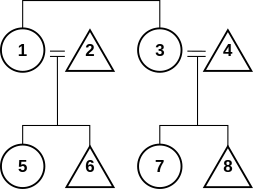
\includegraphics[width = 0.5\linewidth]{figures/kinship_short.pdf}
  \caption{A typical kinship diagram.}
  \label{fig:short-kinship}
\end{figure}

In 1949 the anthropologist G.P. Murdock identified six basic patterns of kinship terminology systems, which are now generally accepted. Of course, certain languages can display systems different from them, but the six types below are the most common ones. 

In order to represent these systems, a diagram like the one in Figure \ref{fig:template-kinship} is used. A shaded triangle or circle, if included, represents the person from whose point of view the tree is presented, called the \textit{Ego} in genealogy.

\begin{figure}[h]
  \includegraphics[width = \linewidth]{figures/kinship_template.pdf}
  \caption{Template kinship diagram for describing the different types of kinship systems.}
  \label{fig:template-kinship}
\end{figure}

The simplest kinship system is called \emph{Hawaiian}, which has only three basic kinship terms: \texttr{mother}, \texttr{father} and \texttr{sibling}. Thus, persons A, D and E are all called \texttr{father}, persons B, C, F are all called \texttr{mother} and all siblings and cousins are called the same (\texttr{sibling}). In this case (the Hawaiian system), we write A = D = E, B = C = F and G = H = I = J = K = L = M = N = O = P. This representation does not take into account the variations based on age so, solely based on this description, we cannot know that in the Hawaiian language (which displays the Hawaiian kinship term) there is a difference between younger and older sibling. Generally, in linguistics problems, if the age does not play a relevant role, it will not be included in the diagram (i.e., if a diagram includes the age of the persons, age will certainly play a role).

The next system is called \emph{Eskimo}\footnote{The term dates from 1949 and is still used even though the word \textit{Eskimo} is now disdained as being derogatory.} kinship (or \emph{Inuit}) one, which is also the system used in English. In this system we differentiate C (\texttr{mother}), D (\texttr{father}), B = F (\texttr{aunt}), A = E (\texttr{uncle}), K = L (\texttr{siblings}) and G = H = I = J = M = N = O = P (\texttr{cousins}). Although the six main kinship systems we describe here represent general patterns, these patterns can be slightly modified from one language to another. A case worth mentioning is that of Romanian which, although it is considered to use an Eskimo kinship term, it has two different words for \texttr{cousin} based on the gender, and differentiates between G = I = M = O (\cmubdata{verișoară}, \texttr{female cousin}) and H = J = N = P (\cmubdata{verișor}, \texttr{male cousin}). This is true of many European languages, and in some (e.g. German) the difference \cmubdata{Kusine}--\cmubdata{Vetter} is not just a gender suffix. 

The next system we talk about is called \emph{Sudanese} kinship, one example of which is Turkish, which we use here to illustrate. In this type of system there is a separate term for each of the persons A-F (\wordtrans{dayı}{mother's brother}, \wordtrans{amca}{father's brother}, \wordtrans{teyze}{mother's sister}, \wordtrans{hala}{father's sister}, \wordtrans{anne}{mother}, \wordtrans{baba}{father}) and a different term for each pair of cousins: I and J are called \texttr{maternal parallel cousins} – \textit{maternal} refers to the fact that they are on the mother's side. The term \textit{parallel} is used because the blood relation is from the same-sex persons (i.e., same-sex siblings) - mother and mother's sister (two women). In the same way, O and P are called \texttr{paternal parallel cousins}, from the father's side and, more exactly, from the father's brother (parallel since it is the father's brother (same sex as the father), not sister). The other two categories are called \texttr{maternal cross cousins} and \texttr{paternal cross cousins}, where \textit{cross} refers to the fact that the blood relation is of opposite-sex persons (mother's brother and father's sister).

This distinction between \textit{parallel} and \textit{cross} cousins is rather common and so relevant that in the next kinship system, called \emph{Iroquois} kinship, B = C (\texttr{mother}) and D = E (\texttr{father}). Here, the same-sex siblings of the parents (i.e., mother's sister and father's brother) are also considered to be `parents'. On the other hand, the opposite-sex siblings of the parents are those called \texttr{uncle} (A) and \texttr{aunt} (F). For this reason, G = H = O = P (\texttr{cousins}) -- since they are the children of the aunt and uncle --, but I = J = K = L = M = N (\texttr{siblings}) – since they are the children of the mother and father. The next two systems are derived from this system.

\begin{sloppypar}
The \emph{Crow} kinship system starts from the Iroquois system, with the only change occurring for the persons O and P (the children of the father's sister). They are called \texttr{aunt} (if it is a girl, so O) or \texttr{father} (P). Thus, in this system, D = E = P (\texttr{father}) and F = O (\texttr{aunt}). The rest of the persons follow the Iroquois system (A = \texttr{uncle}, B = C = \texttr{mother}, G = H = \texttr{cousins}, I = J = K = L = M = N = \texttr{siblings}).
\end{sloppypar}

The last system, called \emph{Omaha} kinship, is the opposite of Crow kinship. In this system, a special role is reserved for the children of the mother's brother (instead of father's sister, as in the Crow system). Like the Crow system, the same-sex child is also called \texttr{uncle} or \texttr{aunt}, depending on their (and Ego's) sex (same sex as Ego), while the opposite-sex child is called \texttr{mother} or \texttr{father}. Therefore, A = H = \texttr{uncle}, B = C = G = \texttr{mother}, D = E = \texttr{father}, F = \texttr{aunt}, I = J = K = L = M = N = \texttr{sibling} and O = P = \texttr{cousins}.

Although the systems are each named after a language, there are other languages which follow each system: for example English has `Eskimo kinship', Bulgarian has `Sudanese kinship'.

A comparative representation of these six types of system is represented below:

\vfill
\noindent
{\small\begin{tabular}{|c|c|c|c|c|c|c|}
\hline
Person & {Hawaiian} & {Eskimo} & {Sudanese} & {Iroquois} & {Crow} & {Omaha} \\ \hline
A & \texttr{father} & \texttr{uncle} & \texttr{mother's brother} & \multicolumn{3}{c|}{\texttr{uncle}}  \\ \hline
B & \multirow{2}{*}{\texttr{mother}} & \texttr{aunt} & \texttr{mother's sister} & \multicolumn{3}{c|}{\multirow{2}{*}{\texttr{mother}}}  \\ \cline{1-1} \cline{3-4}
C &  & \multicolumn{2}{c|}{\texttr{mother}} & \multicolumn{3}{c|}{}  \\ \hline
D & \multirow{2}{*}{\texttr{father}} & \multicolumn{2}{c|}{\texttr{father}} & \multicolumn{3}{c|}{\multirow{2}{*}{\texttr{father}}} \\ \cline{1-1} \cline{3-4}
E &  & \texttr{uncle} & \texttr{father's brother} & \multicolumn{3}{c|}{}  \\ \hline
F & \texttr{mother} & \texttr{aunt} & \texttr{father's sister} & \multicolumn{3}{c|}{\texttr{aunt}} \\ \hline
\end{tabular}
\vfill\pagebreak
\noindent
\begin{tabular}{|c|c|c|c|c|c|c|}
\hline
Person & {Hawaiian} & {Eskimo} & {Sudanese} & {Iroquois} & {Crow} & {Omaha} \\ \hline
G & \multirow{10}{*}{\texttr{sibling}} & \multirow{4}{*}{\texttr{cousin}} & \multirow{2}{*}{\texttr{maternal CC}\footnotemark{}} & \multicolumn{2}{c|}{\multirow{2}{*}{\texttr{cousin}}} & \texttr{mother} \\ \cline{1-1} \cline{7-7} 
H &  &  &  & \multicolumn{2}{c|}{} &  \texttr{uncle} \\ \cline{1-1} \cline{4-7} 
I &  &  & \multirow{2}{*}{\texttr{maternal PC}\footnotemark[\value{footnote}]} & \multicolumn{3}{c|}{\multirow{6}{*}{\texttr{sibling}}} \\ \cline{1-1}
J &  &  &  &  \multicolumn{3}{c|}{} \\ \cline{1-1} \cline{3-4}
K &  & \multicolumn{2}{c|}{\multirow{2}{*}{\texttr{sibling}}}  &  \multicolumn{3}{c|}{} \\ \cline{1-1}
L &  &  \multicolumn{2}{c|}{}  &  \multicolumn{3}{c|}{} \\ \cline{1-1} \cline{3-4}
M &  & \multirow{4}{*}{\texttr{cousin}} & \multirow{2}{*}{\texttr{paternal PC}\footnotemark[\value{footnote}]} &  \multicolumn{3}{c|}{} \\ \cline{1-1}
N &  &  &  &  \multicolumn{3}{c|}{} \\ \cline{1-1} \cline{4-7} 
O &  &  & \multirow{2}{*}{\texttr{paternal CC}\footnotemark[\value{footnote}]} & \multirow{2}{*}{\texttr{cousin}} & \texttr{aunt} & \multirow{2}{*}{\texttr{cousin}} \\ \cline{1-1} \cline{6-6}
P &  &  &  &  & \texttr{father} & \\ \hline
\end{tabular}}
\footnotetext{CC = \texttr{cross cousin}, PC = \texttr{parallel cousin}.}

\begin{problem}{\langnameArawak}{\nameMBoron}{\wordoriginal}
Below you can find part of an Arawak family tree. Three family members – two men and a woman (not necessarily in this order) – describe their family:
\begin{enumerate}\sloppy
    \item \cmubdata{De to Fatan. Onikhan to dajo. Mithakotoan ken Kolhen to dakhithonon. Tholhady to dato. Ematonoa to dathi.}
    \item \cmubdata{De to Sobole. Bokoa to dakhithi. Kolhen ken Moty to dajonon. Balhose ken Konoko to dathinon. Onikhan ken Ylhydaba to dakythynon. Fatan ken Mithakotoan to dajaboathonon. Sareke to dajorodatho. Ematonoa to dadokothi.}
    \item \cmubdata{De to Balhose. Ylhydaba to dajo. Kolhen to daretho. Sobole ken Bokoa to daithinon. Konoko to dakhithi. Moty to dajorodatho. Mithakotoan ken Fatan to darebiathonon. Sareke to dato.}
\end{enumerate}
\largerpage[2]
% \noindent\includegraphics[width = \linewidth]{images/Arawak.png}

\begin{figure}[H]
\includegraphics[width = 0.66\linewidth]{figures/Arawak.pdf}
\end{figure}

\begin{assgts}
\item Supply the tree with names. If multiple options are possible, provide them all. 
\item Three more people (from the same family) describe their family:
\begin{enumerate}[start = 4]\sloppy
    \item \cmubdata{De to Ajonym. Fatan ken Kolhen to \pbblank. Onikhan to dakythy. Mithakotoan to dajo. \pbblank to dadokothi.}
    \item \cmubdata{De to \pbblank. Balhose ken Konoko to daithinon. Holholho ken Sobole ken \pbblank  to dalykynthinon. Moty to dato. \pbblank to dalykyntho.}
    \item \cmubdata{De to Kolhen. \pbblank to dajo. \pbblank to darethi. Ematonoa to \\ \pbblank. Sareke to dato. Sobole ken Bokoa to \pbblank. Konoko to \pbblank.}
\end{enumerate}
\item[] Fill each gap with \textit{exactly one word}. 
\end{assgts}

\begin{tblsWarning}
In the diagram above, triangles represent men and circles represent women. Horizontal lines represent siblings and vertical lines children. The equals sign denotes marriage. 
\end{tblsWarning}
\end{problem}

\begin{mysolution}

Firstly, we look at the structure of the sentences. Each sentence, except for the first, follows the pattern Name \cmubdata{to} X. So we know that X represents the kinship term. We deduce that \wordtrans{ko}{is/are}, and the first sentence most likely means \texttr{I am X}, therefore \wordtrans{de}{I}. Moreover, we notice that if in the rest of the sentences there are more names co-occurring, they are separated by \cmubdata{ken}, so this word most likely means \texttr{and}. Last but not least, we notice that every time that a sentence contains more than one name, the kinship term ends in \cmubdata{non}, so we deduce that the suffix \cmubdata{-non} marks the plural.

Based on this we can make a table in which we show the relations between the persons mentioned in the data:

\begin{longtable}{llll}
\lsptoprule
      & Fatan & Sobole & Balhose \\ \midrule\endfirsthead
\midrule
      & Fatan & Sobole & Balhose \\ \midrule\endhead
Fatan & \cellcolor[HTML]{808080} & \cmubdata{dajaboatho} & \cmubdata{darebiatho} \\ 
Onikhan & \cmubdata{dajo} & \cmubdata{dakythy} &  \\ 
Mithakotoan & \cmubdata{dakhitho} & \cmubdata{dajaboatho} & \cmubdata{darebiatho} \\ 
Kolhen & \cmubdata{dakhitho} & \cmubdata{dajo} & \cmubdata{daretho} \\ 
Tholhady & \cmubdata{dato} &  &  \\ 
Ematonoa & \cmubdata{dathi} & \cmubdata{dadokothi} &  \\ 
Sobole &  & \cellcolor[HTML]{808080} & \cmubdata{daithi} \\ 
Bokoa &  & \cmubdata{dakhithi} & \cmubdata{daithi} \\ 
Moty &  & \cmubdata{dajo} & \cmubdata{dajorodatho} \\ 
Balhose &  & \cmubdata{dathi} & \cellcolor[HTML]{808080} \\ 
Konoko &  & \cmubdata{dathi} & \cmubdata{dakhithi} \\ 
Ylhydaba &  & \cmubdata{dakythy} & \cmubdata{dajo} \\ 
Sareke &  & \cmubdata{dajorodatho} & \cmubdata{dato} \\ 
\lspbottomrule
\end{longtable}

Moreover, we notice that two names are missing: \emph{Ajonym} and \emph{Holholho} (both of them found in task (b)).

Generally, the first step in solving this type of problem, once the table above is made, is assuming that if two persons have the same relation with a third, then those two persons belong to the same generation (e.g., if A and B are \emph{m} to person X -- or X is \emph{m} to persons A and B -- then, most likely, A and B are part of the same generation, i.e., they are on the same level of the tree). In this case, we notice from the diagram that we have three generations: the top one, which has three members, the middle one (siz members) and the bottom one (six members).

Starting with Fatan, we notice that they are the same relation (\cmubdata{dakhitho}) to both Mithakotoan and Kolhen, so we can assume that these two belong to the same generation. Similarly, we deduce that Fatan and Mithakotoan belong to the same generation (since they both are \cmubdata{dajaboatho} to Sobole). Knowing that Mithakotoan and Kolhen as well as Mithakotoan and Fatan belong to the same generation, we can deduce that all three of them are part of the same generation.

Using the same thought process, we get the following pairs of persons belonging to the same generation: Kolhen – Moty (they are \cmubdata{dajo} for Sobole), Balhose – Konoko (\cmubdata{dathi} for Sobole), Fatan – Mithakotoan (\cmubdata{darebiatho} for Balhose), Sobole – Bokoa (\cmubdata{daithi} for Balhose), Onikhan – Ylhydaba (\cmubdata{dakythy} for Sobole).

Collecting all the information, we get: 

\begin{description}[font=\normalfont]
\item[Group 1:] Mithakotoan – Kolhen – Fatan – Moty
\item[Group 2:] Balhose – Konoko
\item[Group 3:] Sobole – Bokoa
\item[Group 4:] Onikhan – Ylhydaba
\end{description}

We need to take into account that two (or more) of these groups can combine to form a generation. Moreover, we know for sure that Group 1 is part of the middle generation since it contains Moty.

Furthermore, we can use task (b) to see if there are any other names that cooccur. In example 5, sentence 3, we notice that Holholho and Sobole appear together. At first sight, it can seem insignificant since we have no information about Holholho in the corpus. However this information is actually extremely important. If we add Holholho to Group 3, then this group will contain three persons. Since Group 1 has four persons and Group 3 has three persons, we certainly know that these two cannot represent the same generation (since there is no generation with seven members), so we deduce that Group 1 and Group 3 belong to different generations.

Let us look now at the kinship term \cmubdata{dajo}. It appears between Sobole (Group 3) and Kolhen (Group 1), so we know that this term spans across generations. The same relation appears between Fatan (Group 1) and Onikhan (Group 4). Based on this, we deduce that Group 4 represents the last separate generation (it does not combine with either Group 1 or Group 3). This might not seem obvious at first, but we know that the relation between a person from Group 3 and a person from Group 1 is the same as the relation between a person from Group 1 and one from Group 4 (we can write this succinctly as G3--G1 = G1--G4). Moreover, we already know that G3 and G1 belong to different generations, so, if G4 belonged to the same generation as G1, then the second relation (the word \cmubdata{dajo} which refers to Kolhen from G1 and Onikhan from G4) would be within the same generation, while this is not true for the first relation (the word \cmubdata{dajo} which refers to G3--G1). If G4 was part of the same generation as G3, then we would have a reciprocal relation (the relation of X to Y uses the same name as the relation of Y to X – but across different generations), which is highly unlikely. The only option left is, therefore, that G4 belongs to a separate generation.

Let us focus now on the relation \cmubdata{dajo}, which appears between Onikhan (G4) and Fatan (G1), as well as between Ylhydaba (G4) and Balhose (G2) (i.e., G4--G1 = G4--G2). From here, we deduce that G2 and G1 belong to the same generation.

Now we can classify the three generations:\largerpage[2]

\begin{description}[font=\normalfont]
    \item[Generation A (Gen. A):] Mithakotoan, Kolhen, Fatan, Moty, Balhose, Konoko
    \item[Generation B (Gen. B):] Sobole, Bokoa, Holholho
    \item[Generation C (Gen. C):] Onikhan, Ylhydaba
\end{description}

For simplicity, we can remake the table, but this time replacing the name with the generation.

\begin{table}[H]
\begin{tabular}{ *4{l} }
\lsptoprule
  & A & B & A \\ \midrule
A & \cellcolor[HTML]{808080} & \cmubdata{dajaboatho} & \cmubdata{darebiatho} \\ 
C & \cmubdata{dajo} & \cmubdata{dakythy} &  \\ 
A & \cmubdata{dakhitho} & \cmubdata{dajaboatho} & \cmubdata{darebiatho} \\ 
A & \cmubdata{dakhitho} & \cmubdata{dajo} & \cmubdata{daretho} \\ 
Tholhady & \cmubdata{dato} &  &  \\ 
Ematonoa & \cmubdata{dathi} & \cmubdata{dadokothi} &  \\ 
B &  & \cellcolor[HTML]{808080} & \cmubdata{daithi} \\ 
B &  & \cmubdata{dakhithi} & \cmubdata{daithi} \\ 
A &  & \cmubdata{dajo} & \cmubdata{dajorodatho} \\ 
A &  & \cmubdata{dathi} & \cellcolor[HTML]{808080} \\ 
A &  & \cmubdata{dathi} & \cmubdata{dakhithi} \\ 
C &  & \cmubdata{dakythy} & \cmubdata{dajo} \\ 
Sareke &  & \cmubdata{dajorodatho} & \cmubdata{dato} \\ 
\lspbottomrule
\end{tabular}
\end{table}

The first observation is that both Tholhady and Sareke have the relation \cmubdata{dato} with respect to Gen. A, so they both belong to the same generation (B or C, since Gen. A already has six members, so it is complete).

The term \cmubdata{dajorodatho} is established between two persons from Gen. A, so it is a kind of relation established within the same generation. Since Sareke uses the same relation with a person from Gen. B, we deduce that Sareke also belongs to Gen. B.

For Ematonoa, we look at the term \cmubdata{dathi}. We have the equivalence: A--B = Ematonoa--A. Since we said we exclude transitive relations, Ematonoa must belong to Gen. C. Thus, the generations become:

\begin{description}[font=\normalfont]
    \item[Gen. A:] Mithakotoan, Kolhen, Fatan, Moty, Balhose, Konoko
    \item[Gen. B:] Sobole, Bokoa, Holholho, Tholhady, Sareke
    \item[Gen. C:] Onikhan, Ylhydaba, Ematonoa
\end{description}

There is only one person unassigned, Ajonym, who surely belongs to Gen. B (since it is the only incomplete generation in terms of the number of members). Moreover, we know the correspondence between the letters A--C and the top/middle/bottom generations. Gen. C is surely the top one, since it has only three members, while Gen. A is the middle one since it contains Moty. Therefore, Gen. B remains and must be the bottom one. The final generations are:

\begin{description}[font=\normalfont]
    \item[Top generation:]  Onikhan, Ylhydaba, Ematonoa
    \item[Middle generation:]  Mithakotoan, Kolhen, Fatan, Moty, Balhose, Konoko
    \item[Bottom generation:]  Sobole, Bokoa, Holholho, Tholhady, Sareke, Ajonym
\end{description}

We expect that the kinship terms established between the middle and the top generation to be \texttr{mother} and \texttr{father} (the other option is something like \texttr{wife's sister's mother}, which is rather too complex). Thus, we notice that for Fatan, Onikhan and Ematonoa are \cmubdata{dathi} and \cmubdata{dajo}, respectively; we can assume that they represent \texttr{mother} and \texttr{father}. Since there is only one married couple in the top generation, it must be Onikhan-Ematonoa. To differentiate between \texttr{mother} and \texttr{father}, we notice that \cmubdata{dajo} also appears with Ylhydaba, who belongs to the top generation. Since the only person left in the top generation is a woman, we deduce that \wordtrans{dajo}{mother} and \wordtrans{dathi}{father}. Moreover, we can assign all the names to the top generation (from left to right: Onikhan, Ematonoa, Ylhydaba).

We notice that for Sobole, both Onikhan and Ylhydaba are \cmubdata{dakythy}. Since Sobole is part of the bottom generation, we can easily deduce that \wordtrans{dakythy}{grandmother}. Moreover, we deduce that Sobole must be one of the children in the middle of the tree (the group of three siblings), since they are the only persons whose grandparents are both Onikhan and Ylhydaba.

Let us now look at Sobole's statements. Since we already know the words for \texttr{mother} and \texttr{father}, we notice that in the generation above, Sobole has two persons who they refer to as \cmubdata{dajo} \texttr{mother} (Kolhen and Moty), two who they call \cmubdata{dathi} \texttr{father} (Konoko and Balhose) and two who they refer to as \cmubdata{dajaboatho} (Fatan and Mithakotoan). Among the two persons called \texttr{mother}, we can surely expect that one of them but not both is their biological mother. Since we already know where Moty is placed, we deduce that Kolhen is the (biological) mother of Sobole (the married woman). Moreover, certainly the two men will be those called \texttr{father} (Konoko and Balhose), and the two remaining women on the right will be Fatan and Mithakotoan. Furthermore, the relation between Fatan and Mithakotoan is \cmubdata{dakhitho}, so \wordtrans{dakhitho}{sister (of a woman)}. Similarly, the relation between Konoko and Balhose is \cmubdata{dakhithi}, so \wordtrans{dakhithi}{brother (of a man)}. Next, we notice the similarity between the two terms, which differ only in terms of their last vowel (\cmubdata{-i} or \cmubdata{-o}), which makes us assume that the difference in gender is marked by the last vowel (thus, the stem \cmubdata{dakhith-} means \texttr{same-sex sibling}; if it ends in the vowel \cmubdata{-i}, meaning masculine, it will refer to same-sex brothers i.e., brother of a male, while if it receives the suffix \cmubdata{-o}, it means same-sex sister, i.e., a woman's sister).

We also notice that Bokoa and Sobole are \cmubdata{dakhithi}, so the two are siblings. Therefore, Sobole and Bokoa are the two men from the bottom generation. Moreover, the two men are \cmubdata{daithi} for Balhose, so \wordtrans{daithi}{son}. We can assume that Balhose is the biological father of the two children (unlike Konoko). This is also confirmed by the fact that Kolhen is \cmubdata{daretho} for Balhose, and this kinship term does not occur again, so it means that \wordtrans{daretho}{wife}.

Sareke is \cmubdata{dato} for Balhose, and Sareke is part of the bottom generation. The only person, in relation with Balhose, which we have not described, is their daughter, so Sareke is the daughter of Balhose (the sister of Sobole and Bokoa), and \wordtrans{dato}{daughter}.

Furthermore, since Tholhady is the daughter of Fatan (knowing that Fatan and Mithakotoan are the two women in the middle generation, and only one of them has a daughter), we can determine all the correspondences of the middle generation. The names are, from left to right: Fatan, Mithakotoan, Kolhen, Balhose, Konoko, Moty.

The only persons left to be assigned to the diagram are Ajomyn and Holholho. Checking task (b), sentence 4, Ajonym says that Onikhan is their \cmubdata{dakythy} \texttr{grandmother}, so Ajonym is the son of Mithakotoan, while Holholho is the son of Moty.

The only thing left undetermined is the difference between Sobole and Bokoa. Since we have no information which could help differentiate between the two (and since task (a) says that there are multiple options in some cases), we deduce that the correct assignment of names is as presented in Figure \ref{fig:arawak-solution} (with the mention that Sobole and Bokoa can be swapped).

\vfill
\begin{figure}[H]
  \includegraphics[width = 0.66\linewidth]{figures/Arawak_withNames.pdf}
  \caption{The name assignment for Problem 10.2.}
  \label{fig:arawak-solution}
\end{figure}
\vfill\pagebreak

Based on this, we can easily deduce the remaining kinship terms, and make a table with all the words we know (since we saw that the masculine-feminine pairs are similar, we organise them in different columns):

\begin{table}[H]
    \begin{tabular}{ lll }
    \lsptoprule
    Kinship term & Male & Female \\\midrule
    \texttr{child} & \cmubdata{daithi} & \cmubdata{dato} \\
    \texttr{parent} or \texttr{father's sibling} & \cmubdata{dathi} & \cmubdata{dajo} \\
    \texttr{grandparent} & \cmubdata{dadokothi} & \cmubdata{dakythy} \\
    \texttr{grandchild} & \cmubdata{dalykynthi} & \cmubdata{dalykyntho} \\
    \texttr{same-sex sibling} & \cmubdata{dakhithi} & \cmubdata{dakhitho} \\
    \texttr{opposite-sex sibling} & \cmubdata{} & \cmubdata{dajorodatho} \\
    \texttr{spouse} & \cmubdata{darethi} & \cmubdata{daretho} \\
    \texttr{spouse's same-sex sibling} & \cmubdata{darebiathi} & \cmubdata{darebiatho} \\
    \texttr{mother's sibling} & \cmubdata{} & \cmubdata{dajaboatho} \\
    \lspbottomrule
    \end{tabular}
\end{table}

We notice again that some kinship terms can switch between masculine and feminine by changing the last vowel from \cmubdata{-i} (masculine) to \cmubdata{-o} (feminine).

Based on this, we can solve task (b):
\begin{multicols}{3}
\begin{enumerate}[label = (\arabic*)]
    \item \cmubdata{dajaboathonon}
    \item \cmubdata{Ematonoa}
    \item \cmubdata{Ylhydaba}
    \item \cmubdata{Bokoa}
    \item \cmubdata{Sareke}
    \item \cmubdata{Onikhan}
    \item \cmubdata{Balhose}
    \item \cmubdata{dathi}
    \item \cmubdata{daithinon}
    \item \cmubdata{darebiathi}
\end{enumerate}
\end{multicols}
\end{mysolution}

\hypertarget{practice-problems}{%
\section{Practice problems}}

\begin{problem}{\langnameBardi}{\nameCSheard}{\LOYear{\UKLOAbbr}{2012}}
In the picture below, note that both you and the speaker are facing the paper. The bird is to the left of everything else and the kangaroo is to the right of everything else. The cat is behind everything else and the kangaroo is in front of everything else.

\begin{center}
\includegraphics[width = 10 cm]{images/Bardi.png}
\end{center}
Here are some Bardi sentences describing the scene:
\begin{enumerate}[label = \roman*), leftmargin = 1in]
    \item \cmubdata{Aamba bornkony yaawardon.}
    \item \cmubdata{Baawa joorroonggony garrabalgoon.}
    \item \cmubdata{Boorroo alaboor yaawardon.}
    \item \cmubdata{Iila alaboor ooranygoon.}
    \item \cmubdata{Iila baybirrony aambon.}
    \item \cmubdata{Minyaw baybirrony baawon.}
    \item \cmubdata{Oorany joorroonggony baawon.}
    \item \cmubdata{Yaawarda bornkony aambon.}
\end{enumerate}
\pagebreak
\begin{assgts}
\item Based on these, determine the following correspondences:
\begin{center}
    \begin{tabular}{rl@{\hskip0.5in}cl}
         \chaosline{Aarlgoodony}{bird}
         \chaosline{Aamba}{child}
         \chaosline{Alaboor}{cat}
         \chaosline{Baawa}{dog}
         \chaosline{Baybirrony}{horse}
         \chaosline{Boorroo}{kangaroo}
         \chaosline{Bornkony}{man}
         \chaosline{Garrabal}{woman}
         \chaosline{Iila}{next to}
         \chaosline{Joorroonggony}{behind}
         \chaosline{Minyaw}{in front of}
         \chaosline{Oorany}{to the left of}
         \chaosline{Yaawarda}{to the right of}
    \end{tabular}
\end{center}
\end{assgts}
\end{problem}

\begin{problem}{\langnameKharia}{\nameBDohnalova}{\LOYear{\CLOAbbr}{2021}}
Below is shown the kinship tree of a Kharia family in which circles represent women and squares represent men. The age of each person is written under their name.
\vfill
\begin{figure}[H]
\includegraphics[width = \linewidth]{figures/Kharia.pdf}
\end{figure}
\vfill\pagebreak

Each member of this family says something about their family in Kharia: 
\begin{enumerate}[label = \alph*.]
    \item \cmubdata{Bhaiiɲaʔ ɲimi Thuyu.}
    \item \cmubdata{Didiiɲaʔ ɲimi Muni. Ɖonkuiiɲaʔ ɲimi Mariya.}
    \item \cmubdata{Sowiɲaʔ ɲimi Nuh.}
    \item \cmubdata{Didikiiɲaʔ ɲimiki Olem oɖoyoʔ no Ewa.}
    \item \cmubdata{Konon bahiniɲaʔ ɲimi Olem. Didikiiɲaʔ ɲimiki Ewa oɖoyoɁ no Kolo.}
    \item \cmubdata{Ɖonkuiiɲaʔ ɲimi Muni. Dad=iɲaʔ ɲimi Dele.}
    \item \cmubdata{Sowiɲaʔ ɲimi Thuyu. Be\textsuperscript{ʔ}ʈiɲaʔ ɲimi Anil.}
    \item \cmubdata{Dadakiiɲaʔ ɲimiki Beni oɖoyoʔ no Sim.}
    \item \cmubdata{Be\textsuperscript{ʔ}ʈiɲaʔ ɲimi Beni. Ɖonkuiiɲaʔ ɲimi Mariya.}
    \item \cmubdata{Bhaikiiɲaʔ ɲimiki Beni oɖoyoʔ no Anil. Apaiɲaʔ ɲimi Dele.}
    \item \cmubdata{Konon bahinkiiɲaʔ ɲimiki Kolo, Ewa oɖoyoʔ no Olem.}
    \item \cmubdata{Konon bahinkiiɲaʔ ɲimiki Muni oɖoyoʔ no Kepka.}
    \item \cmubdata{Apaiɲaʔ ɲimi Nuh. Dad=iɲaʔ ɲimi Sim.}
\end{enumerate}
\begin{assgts}
\item Assign each of the sentences above to the person who uttered it.
\item Fill in the blanks:
\begin{enumerate}[label = \roman*.]
    \item Muni: “\cmubdata{\pbblank ɲimi Dele.}”
    \item Kepka: “\cmubdata{\pbblank ɲimi Nuh.}”
    \item Ewa: “\cmubdata{Konon bahinkiiɲaʔ ɲimiki \pbblank.}”
    \item Anil: “\cmubdata{Dad=iɲaʔ ɲimi  \pbblank.}”
    \item Beni: “\cmubdata{\pbblank ɲimi Dele.}”
\end{enumerate}
\item A few years later, Kepka has a son named Caitu. Fill in the blanks:
\begin{enumerate}[label = \roman*., start = 6]
    \item Sim: “\cmubdata{\pbblank ɲimi Caitu.}”
    \item Kepka: “\cmubdata{\pbblank ɲimi Caitu.}”
    \item Caitu: “\cmubdata{\pbblank ɲimiki Ewa, Olem oɖoyoʔ no Kolo.}”
\end{enumerate}
\end{assgts}
\end{problem}

\begin{problem}{\langnameEmbaloh}{\nameKGilyarova}{\LOYear{\MSKAbbr}{2006}}
A tourist travels to a village on the course of the river Benoit Martinus Ambala (Kalimantan Island, Indonesia), in order to learn the Embaloh language. He will live at the Chief's House (see map). On the first day, the Chief takes his guest outside, points towards the north, south, east and west and says “urait, kalaut, anait, suali”. The tourist wrote down in his own dictionary: \wordtrans{urait}{north}, \wordtrans{kalaut}{south}, \wordtrans{anait}{east}, \wordtrans{suali}{west}.\largerpage[2]

\begin{figure}
\includegraphics[width = \linewidth]{images/Embolah_EN.png}
\end{figure}

The next day, the tourist wanted to visit the Sanctuary – the place where all the important tribal ceremonies take place. He took his dictionary and compass, but he left his map at home. Exiting the Chief's House, he started walking north and reached the Shaman's House. He asked the Shaman: “How can I get to the Sanctuary?”\ “Keep going \cmubdata{urait},”\ replied the Shaman. “So, I should head north”\ thought the tourist, checking his dictionary. He crossed the river, but then he got lost in a Rice Field, so he decided to return to the Shaman. A plantation worker guided him: “Towards the Shaman's House, go \cmubdata{suali}.” “That means west?! Weird!” thought the tourist, but nevertheless he headed west. However, the river didn't come up and the rice fields were slowly replaced by coconut plantations and the tourist realised he was completely lost. “Whatever it is,”\ a worker on the coconut plantation started comforting the tourist, “keep going \cmubdata{kalaut}. You will get to the School and the teacher will explain everything.”

Checking his dictionary, he headed south and he indeed reached the school. “Chief's House \cmubdata{anait}?”\ the tourist asked the teacher. “No, \cmubdata{anait} Diamond Mine. Chief's House \cmubdata{suali}”\ he replied. The tourist, humbled, headed west and found himself at the Diamond Mine. Extremely angry, he asked: “How can I finally reach the Chief's House or at least the School?”\ “Chief's House \cmubdata{suali}, but School \cmubdata{andoor}.”\ Unfortunately, this last word does not appear in the tourist's dictionary.

\begin{assgts}
\item Explain why the tourist got lost and explain how the orientation system of this tribe works, as well as what each direction means.
\item Describe in Embolah the directions:
\begin{enumerate}
    \item from the Sanctuary to the Shaman's House;
    \item from the Bamboo Forest to the Shaman's House;
    \item from the Shaman's House to the Rice Field.
\end{enumerate}
\end{assgts}
\end{problem}\largerpage[2]

\begin{problem}{\langnameHungarian}{\nameAHesterberg}{\LOYear{\UKLOAbbr}{2014}}
The picture below represents a field divided into 49 squares (7x7), aligned with north at the top and east on the right. In some of the squares there are rocks, indicated by a black circle ●. 

\begin{figure}[H]
\includegraphics[width = 6 cm]{figures/Hungarian_Squares.pdf}
\end{figure}

There are four Hungarian friends - A, B, C and D – standing in the field, each in a different square not containing a rock, and each facing in one of the four cardinal directions (north, south, east, west). Each person makes some statements describing the position of the rocks. For instance, A's first statement means \texttr{To the east (behind me) there is one stone}. References to directions are to be understood as describing a single line in the field: \texttr{due east}, \texttr{directly behind me}, and so on. No directions describe a more complex spatial relationship.

\begin{multicols}{2}
\begin{enumerate}[leftmargin = 0.5in, label = \Alph* says:]
    \item \cmubdata{Délre két kő van.}\\ \cmubdata{Keletere (mögöttem) egy kő van.}\\ \cmubdata{Jobbra nincs kő.}
    \item \cmubdata{Délre (balra) nincs kő.} \\ \cmubdata{Északra egy kő van.} \\ \cmubdata{Mögöttem két kő van.}
    \item \cmubdata{Északra (előttem) nincs kő.} \\ \cmubdata{Nyugatra egy kő van.} \\ \cmubdata{Jobbra két kő van.}
    \item \cmubdata{Nyugatra (jobbra) két kő van.} \\ \cmubdata{Északra egy kő van.} \\ \cmubdata{Balra nincs kő.}
\end{enumerate}
\end{multicols}
\begin{assgts}
\item Which square is occupied by each of B, C and D? Draw an arrow (like the one under A) to show the direction they are facing.
\end{assgts}
\end{problem}

\begin{problem}{\langnameTabaq}{\nameDMirea}{\LOYear{\RoLOAbbr}{2017}}
Two linguists, Dr. David Lovelang and Dr. Matt Hateword were studying the language spoken by the Tabaq people in South Sudan. While Dr. Lovelang was focused on the phonology of the language, Dr. Hateword was concerned with the way their kinship system works. To further his studies, he chose ten members of a big family and asked them to say a name first and then use the kinship term they'd use to describe that person. He carefully wrote everything down in a notebook and drew the following diagram:\largerpage[3]

\begin{figure}[H]
\includegraphics[width = 7cm]{figures/Tabaq.pdf}
\end{figure}

Shortly after, Dr. Hateword had to give up on his research, leaving all his scribbles as well as the blank diagram to his colleague. At first, Dr. Lovelang had no clue as to how he could fill in the diagram, but, after a closer look at the information in the notebook, he managed to fill it in.

Here are the scribbles from the notebook:
\begin{multicols}{2}
\begin{description}[font=\normalfont,leftmargin=!,labelwidth={\widthof{Nadwah:}}]
    \item[Rowa:] \cmubdata{ít̪\`{ɛ} t̪\'{ɛ}\`{ɛ}r} \\ \cmubdata{Minni, t̪\`{ɔ}\`{ɔ}d̪\`{ʊ}} \\ \cmubdata{Nadwah, ít̪\`{ɛ}-n-t̪\`{ɔ}\`{ɔ}d̪\`{ʊ}-t̪\'{ɛ}\`{ɛ}r}
    
    \item[Kuwa:] \cmubdata{Salva, \'{ʊ}t̪\'{ɛ}-k\`{ɔ}t̪\`{ʊ}} \\ \cmubdata{Abdalla, t̪\`{ɔ}\`{ɔ}d̪\`{ʊ}} \\ \cmubdata{Rowa, t̪\`{ɔ}\`{ɔ}d̪\`{ʊ}-t̪\'{ɛ}\`{ɛ}r}
    
    \item[Salva:] \cmubdata{Abir, w\'{ɔ}\'{ɔ}} \\ \cmubdata{Malak, áɲá-n-t̪\`{ɔ}\`{ɔ}d̪\`{ʊ}} \\ \cmubdata{Nadwah, ít̪\`{ɛ} t̪\'{ɛ}\`{ɛ}r}
    
    \item[Sihan:] \cmubdata{Sadiq, ít̪\`{ɛ}} \\ \cmubdata{Minni, ít̪\`{ɛ}-n-t̪\`{ɔ}\`{ɔ}d̪\`{ʊ}-k\`{ɔ}t̪\`{ʊ}} \\ \cmubdata{Kuwa, áfá}
    
    \item[Malak:] \cmubdata{Minni, ít̪\`{ɛ}} \\ \cmubdata{Sihan, màà} \\ \cmubdata{Abdalla, t̪íì}
    
    \item[Sadiq:] \cmubdata{Salva, t̪\`{ɔ}\`{ɔ}d̪\`{ʊ}} \\ \cmubdata{Abir, màà} \\ \cmubdata{Sihan, ít̪\`{ɛ} t̪\'{ɛ}\`{ɛ}r}
    
    \item[Minni:] \cmubdata{Rowa, màà} \\ \cmubdata{Sadiq, t̪íì} \\ \cmubdata{Abir, w\'{ɔ}\'{ɔ}}
    
    \item[Nadwah:] \cmubdata{Kuwa, w\'{ɔ}\'{ɔ}} \\ \cmubdata{Abdalla, fáàfá} \\ \cmubdata{Rowa, áɲá}
    
    \item[Abir:] \cmubdata{Malak, \'{ʊ}t̪\'{ɛ}} \\ \cmubdata{Nadwah, \'{ʊ}t̪\'{ɛ}} \\ \cmubdata{Sadiq, t̪\`{ɔ}\`{ɔ}\textsubbridge{d}\`{ʊ}-k\`{ɔ}t̪\`{ʊ}}
    
    \item[Abdalla:] \cmubdata{Kuwa, áfá} \\ \cmubdata{Malak, ít̪\`{ɛ}-n-t̪\`{ɔ}\`{ɔ}d̪\`{ʊ}} \\ \cmubdata{Salva, ít̪\`{ɛ}-n-t̪\`{ɔ}\`{ɔ}\textsubbridge{d}\`{ʊ}-k\`{ɔ}t̪\`{ʊ}}
\end{description}
\end{multicols}

While filling in the diagram, Dr. Lovelang noticed that, in Tabaq, certain kinship terms can be expressed using two different terms, and one of them is derived from the other. Moreover, he noticed somewhere in the notebook the following information: \textit{Sadiq is a man.} and \textit{Rowa has children.}

\begin{assgts}
\multicolsep=3pt\largerpage[2.5]
\item Fill in the diagram above with the names of the ten family members (in the diagram above circles represents women and squares men). 
\item Write in Tabaq all the possible kinship terms that denote the relation between the following persons:

\begin{multicols}{2}\raggedcolumns
\begin{enumerate}[label = \alph*.]
    \item Sadiq to Salva 
    \item Abir to Nadwah
    \item Salva to Sihan
    \item Nadwah to Minni\columnbreak
    \item Malak to Kuwa
    \item Abdalla to Rowa
    \item Abdalla to Salva
\end{enumerate}
\end{multicols}

\end{assgts}
\end{problem}

\begin{problem}{\langnameAralle}{\nameKGilyarova}{\LOYear{\IOLAbbr}{2016}}
A linguist came to Salu Leang (Sulawesi) to study the Aralle-Tabulahan language. He visited various hamlets of Salu Leang (see the map below) and asked local residents: \cmubdata{Umba laungngola?} \texttr{Where are you going?}

\begin{figure}[H]
\includegraphics[width=0.75\linewidth]{images/Aralle_EN.jpg}
\end{figure}

Below are the answers he got. There are gaps in some of them.

% % \begin{multicols}{2}
\begin{itemize}[noitemsep]
    \item In {Kahangang} hamlet:
    \begin{itemize}
    \item \cmubdata{Lamaoä' bete' di Bulung.}
    \item \cmubdata{Lamaoä' sau di Kota.}
    \item \cmubdata{Lamaoä' \pbblank di Palempang.}
    \end{itemize}
    \item In {Kombeng} hamlet:
    \begin{itemize}
    \item \cmubdata{Lamaoä' pano di Pahihuang.}
    \item \cmubdata{Lamaoä' tama di Sohongang.}
    \item \cmubdata{Lamaoä' naung di Tamonseng.}
    \item \cmubdata{Lamaoä' \pbblank di Palempang.}
    \end{itemize}
    \item In {Kota} hamlet:
    \begin{itemize}
    \item \cmubdata{Lamaoä' dai' di Kombeng.}
    \item \cmubdata{Lamaoä' dai' di Palempang.}
    \item \cmubdata{Lamaoä' naung di Pikung.}
    \item \cmubdata{Lamaoä' \pbblank di Bulung.}
    \item \cmubdata{Lamaoä' \pbblank di Sohongang.}
    \end{itemize}
    \item In {Palempang} hamlet:
    \begin{itemize}
    \item \cmubdata{Lamaoä' bete' di Kahangang.}
    \item \cmubdata{Lamaoä' dai' di Kombeng.}
    \item \cmubdata{Lamaoä' pano di Panampo.}
    \item \cmubdata{Lamaoä' sau di Sohongang.}
    \item \cmubdata{Lamaoä' \pbblank di Bulung.}
    \item \cmubdata{Lamaoä' \pbblank di Kota.}
    \item \cmubdata{Lamaoä' \pbblank di Pahihuang.}
    \end{itemize}
    \item In {Pahihuang} hamlet:
    \begin{itemize}
    \item \cmubdata{Lamaoä' naung di Bulung.}
    \item \cmubdata{Lamaoä' naung di Pikung.}
    \end{itemize}
    \item In {Bulung} hamlet:
    \begin{itemize}
    \item \cmubdata{Lamaoä' pano di Pahihuang.}
    \item \cmubdata{Lamaoä' pano di Panampo.}
    \item \cmubdata{Lamaoä' \pbblank di Kota.}
    \item \cmubdata{Lamaoä' \pbblank di Pikung.}
    \end{itemize}
    \item In {Panampo} hamlet:
    \begin{itemize}
    \item \cmubdata{Lamaoä' tama di Kahangang.}
    \item \cmubdata{Lamaoä' pano di Tamonseng.}
    \item \cmubdata{Lamaoä' \pbblank di Kota.}
    \end{itemize}
    \item In {Pikung} hamlet:
    \begin{itemize}
    \item \cmubdata{Lamaoä' pano di Kota.}
    \item \cmubdata{Lamaoä' dai' di Pahihuang.}
    \item \cmubdata{Lamaoä' sau di Sohongang.}
    \item \cmubdata{Lamaoä' \pbblank di Bulung.}
    \item \cmubdata{Lamaoä' \pbblank di Kahangang.}
    \item \cmubdata{Lamaoä' \pbblank di Panampo.}
    \end{itemize}
    \item In {Sohongang} hamlet:
    \begin{itemize}
    \item \cmubdata{Lamaoä' bete' di Bulung.}
    \item \cmubdata{Lamaoä' tama di Kahangang.}
    \item \cmubdata{Lamaoä' tama di Kota.}
    \item \cmubdata{Lamaoä' dai' di Pahihuang.}
    \end{itemize}
    \item In {Tamonseng} hamlet:
    \begin{itemize}
    \item \cmubdata{Lamaoä' pano di Pahihuang.}
    \item \cmubdata{Lamaoä' pano di Panampo}
    \item \cmubdata{Lamaoä' \pbblank di Kahangang.}
    \item \cmubdata{Lamaoä' \pbblank di Palempang.}
    \end{itemize}
\end{itemize}
% % \end{multicols}
\begin{assgts}
\item \fillblanks
\end{assgts}
\end{problem}

\begin{problem}{\langnameAkan}{\nameKGilyarova}{\LOYear{\IOLAbbr}{2018}}
Below three Akan men who belong to one family introduce themselves and some members of their family (see the family tree): 
\begin{enumerate}
    \item \cmubdata{Yɛfrɛ me Enu. Yɛfrɛ me banom Thema ne Yaw ne Ama. Yɛfrɛ me yere Kunto. Yɛfrɛ me nuanom Awotwi ne Nsia. Yɛfrɛ me wɔfaase Berko.}
    \item \cmubdata{Yɛfrɛ me Kofi. Yɛfrɛ me nua Esi. Yɛfrɛ me agya Ofori. Yɛfrɛ me se\-waa\-nom Dubaku ne Kunto. Yɛfrɛ me sewaabanom Yaw ne Ama ne Kobina.}
    \item \cmubdata{Yɛfrɛ me Kobina. Yɛfrɛ me ɛnanom Dubaku ne Kunto. Yɛfrɛ me nuanom Yaw ne Ama. Yɛfrɛ me wɔfa Ofori. Yɛfrɛ me yere Efua.}
\end{enumerate}

\begin{figure}[H]
\includegraphics[width = \textwidth]{figures/akan.pdf}\smallskip\\
\includegraphics[width = 0.8\textwidth]{figures/akan_legend.pdf}
\end{figure}

\begin{assgts}
\item Supply the family tree with names.
\item Here are some more statements by two other men from this family:
\begin{enumerate}[start = 4]\sloppy
    \item \cmubdata{Yɛfrɛ me Yaw. Yɛfrɛ me ɛnanom \pbblank. Yɛfrɛ me \pbblank Nsia ne \pbblank. Yɛfrɛ me nuanom Thema ne \pbblank. Yɛfrɛ me \pbblank A\-wot\-wi. Yɛfrɛ me \pbblank Ofori. Yɛfrɛ me \pbblank Esi ne \pbblank. Yɛ\-frɛ me \pbblank Berko.}
    \item \cmubdata{Yɛfrɛ me \pbblank. Yɛfrɛ me banom Kofi ne \pbblank. Yɛ\-frɛ me\\ \pbblank \-Yaw ne \pbblank. Yɛfrɛ me \pbblank Kunto ne \pbblank.}
\end{enumerate}
\item[] Fill in the gaps. Some gaps contain more than one word.
\end{assgts}
\end{problem}

\hypertarget{solutions-of-practice-problems}{%
\section{Solutions of practice problems}}

\begin{practiceproblemsolution}{10.3. \langnameBardi}

\begin{solutions}[label=Solution 10.3\alph*]
    \item 1-l, 2-g, 3-k, 4-b, 5-j, 6-f, 7-i, 8-a, 9-d, 10-m, 11-c, 12-h, 13-e.
\end{solutions}
\end{practiceproblemsolution}


\begin{practiceproblemsolution}{10.4. \langnameKharia}

\begin{solutions}[label=Solution 10.4\alph*]
    \item
    \begin{multicols}{3}
        \begin{enumerate}[label = \alph*.]
            \item Dele
            \item Kepka
            \item Mariya
            \item Anil
            \item Beni
            \item Thuyu
            \item Rut
            \item Olem
            \item Muni
            \item Ewa
            \item Sim
            \item Nuh
            \item Kolo
        \end{enumerate}
    \end{multicols}
    \item
    \begin{multicols}{2}
        \begin{enumerate}
            \item \cmubdata{Sowiɲaʔ}
            \item \cmubdata{Dad=iɲaʔ}
            \item \cmubdata{Kolo oɖoyoʔ no Olem}
            \item \cmubdata{Beni}
            \item \cmubdata{Apaiɲaʔ}
            \item[]
        \end{enumerate}
    \end{multicols}
    \item
        \begin{multicols}{3}
        \begin{enumerate}[start = 6]
            \item \cmubdata{Bhaiiɲaʔ}
            \item \cmubdata{Be\textsuperscript{ʔ}ʈiɲaʔ}
            \item \cmubdata{Didikiiɲaʔ}
        \end{enumerate}
    \end{multicols}
\end{solutions}

\rules

Sentence structure: [Kinship term]--(\textsc{pl})--\cmubdata{iɲaʔ} \cmubdata{ɲimi}--(\textsc{pl}) [Persons]
\begin{enumerate}
        \item \textsc{pl} = \cmubdata{-ki-} = plural marker (if there is more than one person)
        \item Persons: Their names; if it's more than one person, \wordtrans{oɖoyoʔ no}{and} is added before the last one.
        \item Kinship terms:

        \begin{multicols}{2}
            \begin{itemize}
                \item \wordtrans{bhai}{younger brother}
                \item \wordtrans{dad=}{older brother} (plural: \cmubdata{dadaki})
                \item \wordtrans{konon bahin}{younger sister}
                \item \wordtrans{didi}{older sister}
                \item \wordtrans{be\textsuperscript{ʔ}ʈ}{son}
                \item \wordtrans{apa}{father}
                \item \wordtrans{sow}{husband}
                \item \wordtrans{đonkui}{brother's wife}
            \end{itemize}
        \end{multicols}
\end{enumerate}

\end{practiceproblemsolution}


\begin{practiceproblemsolution}{10.5. \langnameEmbaloh}

\begin{solutions}[label=Solution 10.5\alph*]
    \item On the first day, when he was told the four directions, he automatically assumed that they represented cardinal directions. In reality, they are based on the topography of the area and represent the relative positions with respect to the river. As such:
        \begin{itemize}
            \item[] \wordtrans{andoor}{towards (closer to) the river}
            \item[] \wordtrans{anait}{away from the river}
            \item[] \wordtrans{urait}{upstream}
            \item[] \wordtrans{kalaut}{downstream}
            \item[] \wordtrans{suali}{across the river}
        \end{itemize}
    \item
    \begin{multicols}{3}
        \begin{enumerate}
            \item \cmubdata{kalaut}
            \item \cmubdata{andoor}
            \item \cmubdata{suali}
        \end{enumerate}
    \end{multicols}
\end{solutions}
\end{practiceproblemsolution}



\begin{practiceproblemsolution}{10.6. \langnameHungarian}

\begin{center}
\includegraphics[width = 8 cm]{figures/Hungarian_Squares_solution.pdf}
\end{center}
\begin{multicols}{3}
\begin{itemize}[noitemsep]
    \item[] \wordtrans{előttem}{front}
    \item[] \wordtrans{mögöttem}{back}
    \item[] \wordtrans{balra}{left}
    \item[] \wordtrans{jobbra}{right}
    \item[] \wordtrans{északra}{north}
    \item[] \wordtrans{délre}{south}
    \item[] \wordtrans{nyugatra}{west}
    \item[] \wordtrans{keletere}{east}
    \item[] \wordtrans{nincs}{0}
    \item[] \wordtrans{egy}{1}
    \item[] \wordtrans{két}{2}
    \item[] \quad
\end{itemize}
\end{multicols}
\end{practiceproblemsolution}



\begin{practiceproblemsolution}{10.7. \langnameTabaq}

\begin{solutions}[label=Solution 10.7\alph*]
    \item The names in the diagram are, from left to right:

    \begin{itemize}
        \item[] Top generation: Abir, Kuwa
        \item[] Middle generation: Sihan, Rowa, Sadiq, Abdalla
        \item[] Bottom generation: Malak, Minni, Nadwah, Salva
    \end{itemize}
    \item
    \begin{enumerate}[label = \alph*.]

        \item \cmubdata{áfá}
        \item \cmubdata{wɔ́ɔ́}
        \item \cmubdata{ít̪ɛ̀-n-t̪ɔ̀ɔ̀d̪ʊ̀} or \cmubdata{ít̪ɛ̀-n-t̪ɔ̀ɔ̀d̪ʊ̀-kɔ̀t̪ʊ̀}
        \item \cmubdata{tíì-n-t̪ɔ̀ɔ̀d̪ʊ̀} or \cmubdata{tíì-n-t̪ɔ̀ɔ̀d̪ʊ̀-t̪ɛ́ɛ̀r}
        \item \cmubdata{ʊ́t̪ɛ́} or \cmubdata{ʊ́t̪ɛ́-t̪ɛ́ɛ̀r}
        \item \cmubdata{ít̪ɛ̀} or \cmubdata{ít̪ɛ̀-kɔ̀t̪ʊ̀}
        \item \cmubdata{fáàfá}
    \end{enumerate}
\end{solutions}

\rules

The kinship terms are:
\begin{multicols}{2}
    \begin{itemize}
        \item[] \cmubdata{ít̪ɛ̀}* = \texttr{sibling}
        \item[] \cmubdata{t̪ɔ̀ɔ̀d̪ʊ}* = \texttr{child}
        \item[] \cmubdata{ʊ́t̪ɛ́}* = \texttr{grandchild}
        \item[] \cmubdata{ít̪ɛ̀-n-t̪ɔ̀ɔ̀d̪ʊ̀}* = \texttr{nephew, niece}
        \item[] \wordtrans{wɔ́ɔ́}{grandparent}
        \item[] \wordtrans{áɲá}{father's sister}
        \item[] \wordtrans{màà}{mother, mother's sister}
        \item[] \wordtrans{fáàfá}{father's brother}
        \item[] \wordtrans{tíì}{mother's brother}
        \item[] \wordtrans{áfá}{father}
    \end{itemize}
\end{multicols}

The words marked with * can receive the suffixes \cmubdata{-t̪ɛ́ɛ̀r} and \cmubdata{-kɔ̀t̪ʊ̀}, in order to mark the gender (feminine and masculine, respectively).

The structure \cmubdata{X-n-t̪ɔ̀ɔ̀d̪ʊ} is translated as \texttr{X's child} (thus, a nephew/niece is actually translated as the \texttr{child of the sibling}). The words \cmubdata{màà}, \cmubdata{áɲá}, \cmubdata{tíì}, and \cmubdata{fáàfá} can be combined with \cmubdata{-n-t̪ɔ̀ɔ̀d̪ʊ̀} to express \texttr{cousin}.\\

\end{practiceproblemsolution}


\begin{practiceproblemsolution}{10.8. \langnameAralle}

\begin{solutions}[label=Solution 10.8\alph*]
    \item
    \begin{multicols}{4}
        \begin{enumerate}

            \item \cmubdata{dai'}
            \item \cmubdata{dai'}
            \item \cmubdata{bete'}
            \item \cmubdata{sau}
            \item \cmubdata{naung}
            \item \cmubdata{sau}
            \item \cmubdata{naung}
            \item \cmubdata{tama}
            \item \cmubdata{naung}
            \item \cmubdata{pano}
            \item \cmubdata{bete'}
            \item \cmubdata{tama}
            \item \cmubdata{dai'}
            \item \cmubdata{bete'}
            \item \cmubdata{dai'}
            \item[] \quad
        \end{enumerate}
    \end{multicols}
\end{solutions}

\rules

Basic directions are:
\begin{multicols}{2}
    \begin{itemize}

        \item[] \wordtrans{bete'}{across the river}
        \item[] \wordtrans{tama}{upstream}
        \item[] \wordtrans{sau}{downstream}
        \item[] \wordtrans{pano}{on a flat road}
        \item[] \wordtrans{dai'}{upwards}
        \item[] \wordtrans{naung}{downwards}
    \end{itemize}
\end{multicols}

\end{practiceproblemsolution}


\begin{practiceproblemsolution}{10.9. \langnameAkan}

\begin{solutions}[label=Solution 10.9\alph*]
    \item \quad

    \noindent\includegraphics[width = \linewidth]{figures/akan_solutions.pdf}
    \item
    \begin{multicols}{2}
        \begin{enumerate}[leftmargin = 2em, label = (\arabic*)]
            \item \cmubdata{Dubaku ne Kunto}
            \item \cmubdata{agyanom}
            \item \cmubdata{Enu}
            \item \cmubdata{Ama ne Kobina}
            \item \cmubdata{sewaa}
            \item \cmubdata{wɔfa}
            \item \cmubdata{wɔfabanom}
            \item \cmubdata{Kofi}
            \item \cmubdata{sewaaba}
            \item \cmubdata{Ofori}
            \item \cmubdata{Esi}
            \item \cmubdata{wɔfaasenom}
            \item \cmubdata{Ama ne Kobina}
            \item \cmubdata{nuanom}
            \item \cmubdata{Dubako}
        \end{enumerate}
    \end{multicols}
\end{solutions}

\rules
\begin{itemize}
    \item \wordtrans{Yɛfrɛ me N.}{My name is N.}
    \item \wordtrans{Yɛfrɛ me R N.}{My R's name is N.} (\cmubdata{R} = kinship term)
    \item \wordtrans{X ne Y}{X and Y}
    \item \cmubdata{-nom} = \textsc{pl}
    \item Kinship terms:
    \begin{multicols}{2}
    \begin{itemize}
        \raggedright
        \item \wordtrans{ɛna}{mother, mother's sister}
        \item \wordtrans{wɔfaase}{sister's child}
        \item \wordtrans{sewaa}{father's sister}
        \item \wordtrans{sewaaba}{father's sister's child}
        \item \wordtrans{nua}{sibling, parallel cousin}
        \item \wordtrans{agya}{father, father's brother}
        \item \wordtrans{ba}{child, brother's child}
        \item \wordtrans{wɔfa}{mother's brother}
        \item \wordtrans{wɔfaba}{mother's brother's child}
        \item \wordtrans{yere}{wife}
    \end{itemize}
    \end{multicols}
\end{itemize}
\end{practiceproblemsolution}

% \section{Further reading}
% \begin{enumerate}[{label=[\arabic{*}]}]
%     \item Dousset, Laurent. “Australian aboriginal kinship: an introductory handbook with particular emphasis on the Western Desert.”\ \textit{Pacific-Credo Publications}, Marseilles (2012).
%     \item Fortescue, Michael. “Orientation systems of the North Pacific Rim.”\ \textit{The University of Chicago Press}, Chicago (2011).
%     \item Levinson, Stephen C. “Space in language and cognition: explorations in cognitive diversity.”\ \textit{Cambridge University Press}, Cambridge (2003).
%     \item Parkin, Robert. “How Kinship Systems Change.”\ \textit{Berghahn Books}, New York (2021).
% \end{enumerate}
\nocite{Dousset2012, Fortescue2011, Levinson2003, Parkin2021}
% \printbibliography[heading=FurtherReading]
\FurtherReadingBox{}
\end{refsection}


\appendix
\chapter[Data about the languages featured in the problems]{Data about the languages featured in the problems: Family, number of native speakers, region}
\label{appendix:1}

% \noindent
% \begin{longtable}{|l|m{5.8em}|m{6em}|m{3.5em}|m{8em}|}
% \hline
% \rotatebox[origin=c]{90}{Prob. No.} & {Language} & {Family}\footnote{IE = \famIndoEuropean, TNG = \famTNG.} & {NS}\footnote{Native speakers. bil. = billion, mil. = million, ? = unknown.} & {Region} \\ \hline
\begin{description}[font=\normalfont,style=nextline]\multicolsep=0pt\columnsep=-1em
\item[\langnameAcehnese] 
 \begin{multicols}{2}\begin{description}[font=\normalfont\itshape,noitemsep] 
 \item[]
 \item[\pbnumberabbr] 5.8 
 \item[\family] \famAustronesian 
 \item[]
\item[\nativespeakers] 3.37 mil. 
 \item[\region] \regionIndonesia 
 \end{description}\end{multicols}
\item[\langnameAfrihili] 
 \begin{multicols}{2}\begin{description}[font=\normalfont\itshape,noitemsep] 
 \item[] 
 \item[\pbnumberabbr] 5.12 
 \item[\family] \famConstructed 
 \item[]
\item[\nativespeakers] 0 
 \item[\region] --
 \end{description}\end{multicols}
\item[\langnameAinu] 
 \begin{multicols}{2}\begin{description}[font=\normalfont\itshape,noitemsep] 
 \item[] 
 \item[\pbnumberabbr] 6.13 
 \item[\family] \famIsolated 
 \item[]
\item[\nativespeakers] 2 
 \item[\region] \regionHokkaido\ \Brackets{\regionJapan} 
 \end{description}\end{multicols}
\item[\langnameAkan] 
 \begin{multicols}{2}\begin{description}[font=\normalfont\itshape,noitemsep] 
 \item[] 
 \item[\pbnumberabbr] 10.9 
 \item[\family] \famNigerCongo 
 \item[]
\item[\nativespeakers] 11 mil. 
 \item[\region] \regionGhana\EnumComma\regionIvoryCoast\EnumComma\regionTogo 
 \end{description}\end{multicols}
\item[\langnameAlabama] 
 \begin{multicols}{2}\begin{description}[font=\normalfont\itshape,noitemsep] 
 \item[] 
 \item[\pbnumberabbr] 5.8  
 \item[\family] \famMuskogean 
 \item[]
\item[\nativespeakers] 370 
 \item[\region] \regionTexas\ \Brackets{\regionUSA}
 \end{description}\end{multicols}
\item[\langnameAlamblak] 
 \begin{multicols}{2}\begin{description}[font=\normalfont\itshape,noitemsep] 
 \item[] 
 \item[\pbnumberabbr] 9.14 
 \item[\family] \famSepik 
 \item[]
\item[\nativespeakers] 1,500 
 \item[\region] \regionPNG 
 \end{description}\end{multicols}
\item[\langnameArabic] 
 \begin{multicols}{2}\begin{description}[font=\normalfont\itshape,noitemsep] 
 \item[] 
 \item[\pbnumberabbr] 2.9\EnumComma4.9\EnumComma7.7 
 \item[\family] \famAfroasiatic 
 \item[]
\item[\nativespeakers] 350 mil. 
 \item[\region] \regionAsia\EnumComma\regionAfrica 
 \end{description}\end{multicols}

\pagebreak
\item[\langnameAralle] 
 \begin{multicols}{2}\begin{description}[font=\normalfont\itshape,noitemsep] 
 \item[] 
 \item[\pbnumberabbr] 10.8 
 \item[\family] \famAustronesian 
 \item[]
\item[\nativespeakers] 12,000 
 \item[\region] \regionWSulawesi\ \Brackets{\regionIndonesia} 
 \end{description}\end{multicols}
\item[\langnameArawak] 
 \begin{multicols}{2}\begin{description}[font=\normalfont\itshape,noitemsep] 
 \item[] 
 \item[\pbnumberabbr] 10.2 
 \item[\family] \famArawakan 
 \item[]
\item[\nativespeakers] 2,510 
 \item[\region] \regionSouthAmerica 
 \end{description}\end{multicols}
\item[\langnameArmenian] 
 \begin{multicols}{2}\begin{description}[font=\normalfont\itshape,noitemsep] 
 \item[] 
 \item[\pbnumberabbr] 2.5 
 \item[\family] \famIndoEuropean 
 \item[]
\item[\nativespeakers] 6.7 mil. 
 \item[\region] \regionArmenia 
 \end{description}\end{multicols}
\item[\langnameBardi] 
 \begin{multicols}{2}\begin{description}[font=\normalfont\itshape,noitemsep] 
 \item[] 
 \item[\pbnumberabbr] 10.3 
 \item[\family] \famNyulnyulan 
 \item[]
\item[\nativespeakers] 4 
 \item[\region] \regionAustralia 
 \end{description}\end{multicols}
\item[\langnameBari] 
 \begin{multicols}{2}\begin{description}[font=\normalfont\itshape,noitemsep] 
 \item[] 
 \item[\pbnumberabbr] 4.13\EnumComma5.8 
 \item[\family] \famNiloSaharan 
 \item[]
\item[\nativespeakers] 750,000 
 \item[\region] \regionSSudan 
 \end{description}\end{multicols}
\item[\langnameBasque] 
 \begin{multicols}{2}\begin{description}[font=\normalfont\itshape,noitemsep] 
 \item[] 
 \item[\pbnumberabbr] 8.3 
 \item[\family] \famIsolated 
 \item[]
\item[\nativespeakers] 750,000 
 \item[\region] \regionFrance\EnumComma\regionSpain 
 \end{description}\end{multicols}
\item[\langnameBeja] 
 \begin{multicols}{2}\begin{description}[font=\normalfont\itshape,noitemsep] 
 \item[] 
 \item[\pbnumberabbr] 7.4 
 \item[\family] \famAfroasiatic 
 \item[]
\item[\nativespeakers] 1-2 mil. 
 \item[\region] \regionSudan\EnumComma\regionEritrea\EnumComma\regionEgypt 
 \end{description}\end{multicols}
\item[\langnameBulgarian] 
 \begin{multicols}{2}\begin{description}[font=\normalfont\itshape,noitemsep] 
 \item[] 
 \item[\pbnumberabbr] 5.4 
 \item[\family] \famIndoEuropean 
 \item[]
\item[\nativespeakers] 8 mil. 
 \item[\region] \regionBulgaria 
 \end{description}\end{multicols}
\item[\langnameBurushaski] 
 \begin{multicols}{2}\begin{description}[font=\normalfont\itshape,noitemsep] 
 \item[] 
 \item[\pbnumberabbr] 7.11 
 \item[\family] \famIsolated 
 \item[]
\item[\nativespeakers] 112,000 
 \item[\region] \regionPakistan 
 \end{description}\end{multicols}
\item[\langnameChabu] 
 \begin{multicols}{2}\begin{description}[font=\normalfont\itshape,noitemsep] 
 \item[] 
 \item[\pbnumberabbr] 9.15 
 \item[\family] \famIsolated 
 \item[]
\item[\nativespeakers] 400 
 \item[\region] \regionEthiopia 
 \end{description}\end{multicols}
\item[\langnameChickasaw] 
 \begin{multicols}{2}\begin{description}[font=\normalfont\itshape,noitemsep] 
 \item[] 
 \item[\pbnumberabbr] 3.8 
 \item[\family] \famMuskogean 
 \item[]
\item[\nativespeakers] 75 
 \item[\region] \regionSOklahoma\ \Brackets{\regionUSA}
 \end{description}\end{multicols}

\pagebreak
\item[\langnameChinese] 
 \begin{multicols}{2}\begin{description}[font=\normalfont\itshape,noitemsep] 
 \item[] 
 \item[\pbnumberabbr] 8.5 
 \item[\family] \famSinoTibetan 
 \item[]
\item[\nativespeakers] 1.2 bil. 
 \item[\region] \regionChina 
 \end{description}\end{multicols}
\item[\langnameChuvash] 
 \begin{multicols}{2}\begin{description}[font=\normalfont\itshape,noitemsep] 
 \item[] 
 \item[\pbnumberabbr] 3.4 
 \item[\family] \famTurkic 
 \item[]
\item[\nativespeakers] 1 mil. 
 \item[\region] \regionRussia 
 \end{description}\end{multicols}
\item[\langnameCree] 
 \begin{multicols}{2}\begin{description}[font=\normalfont\itshape,noitemsep] 
 \item[] 
 \item[\pbnumberabbr] 6.12 
 \item[\family] \famAlgic 
 \item[]
\item[\nativespeakers] 96,000 
 \item[\region] \regionCanada\EnumComma\regionUSA 
 \end{description}\end{multicols}
\item[\langnameTicuna] 
 \begin{multicols}{2}\begin{description}[font=\normalfont\itshape,noitemsep] 
 \item[] 
 \item[\pbnumberabbr] 4.14 
 \item[\family] \famIsolated 
 \item[]
\item[\nativespeakers] 63,000 
 \item[\region] \regionBrazil\EnumComma\regionColumbia\EnumComma\regionPeru 
 \end{description}\end{multicols}
\item[\langnameCzech] 
 \begin{multicols}{2}\begin{description}[font=\normalfont\itshape,noitemsep] 
 \item[] 
 \item[\pbnumberabbr] 9.7 
 \item[\family] \famIndoEuropean 
 \item[]
\item[\nativespeakers] 14 mil. 
 \item[\region] \regionCzechia 
 \end{description}\end{multicols}
\item[\langnameDabida] 
 \begin{multicols}{2}\begin{description}[font=\normalfont\itshape,noitemsep] 
 \item[] 
 \item[\pbnumberabbr] 6.2 
 \item[\family] \famNigerCongo 
 \item[]
\item[\nativespeakers] 370,000 
 \item[\region] \regionKenya 
 \end{description}\end{multicols}
\item[\langnameDanish] 
 \begin{multicols}{2}\begin{description}[font=\normalfont\itshape,noitemsep] 
 \item[] 
 \item[\pbnumberabbr] 9.9 
 \item[\family] \famIndoEuropean 
 \item[]
\item[\nativespeakers] 6 mil. 
 \item[\region] \regionDenmark 
 \end{description}\end{multicols}
\item[\langnameDaza] 
 \begin{multicols}{2}\begin{description}[font=\normalfont\itshape,noitemsep] 
 \item[] 
 \item[\pbnumberabbr] 5.8 
 \item[\family] \famNiloSaharan 
 \item[]
\item[\nativespeakers] 380,000 
 \item[\region] \regionChad\EnumComma\regionNiger\EnumComma\regionSudan\EnumComma\regionLibya 
 \end{description}\end{multicols}
\item[\langnameDinka] 
 \begin{multicols}{2}\begin{description}[font=\normalfont\itshape,noitemsep] 
 \item[] 
 \item[\pbnumberabbr] 6.15 
 \item[\family] \famNiloSaharan 
 \item[]
\item[\nativespeakers] 1.3 mil. 
 \item[\region] \regionSudan 
 \end{description}\end{multicols}
\item[\langnameDutch] 
 \begin{multicols}{2}\begin{description}[font=\normalfont\itshape,noitemsep] 
 \item[] 
 \item[\pbnumberabbr] 4.11 
 \item[\family] \famIndoEuropean 
 \item[]
\item[\nativespeakers] 25 mil. 
 \item[\region] \regionNetherlands 
 \end{description}\end{multicols}
\item[\langnameDyirbal] 
 \begin{multicols}{2}\begin{description}[font=\normalfont\itshape,noitemsep] 
 \item[] 
 \item[\pbnumberabbr] 7.2 
 \item[\family] \famPamaNyungan 
 \item[]
 \item[]
\item[\nativespeakers] 8 
 \item[\region] \regionNEQueensland\ \Brackets{\regionAustralia}
 \end{description}\end{multicols}
\item[\langnameEmbaloh] 
 \begin{multicols}{2}\begin{description}[font=\normalfont\itshape,noitemsep] 
 \item[] 
 \item[\pbnumberabbr] 10.5 
 \item[\family] \famAustronesian 
 \item[]
\item[\nativespeakers] 10,000 
 \item[\region] \regionIndonesia 
 \end{description}\end{multicols}
\item[\langnameChami] 
 \begin{multicols}{2}\begin{description}[font=\normalfont\itshape,noitemsep] 
 \item[] 
 \item[\pbnumberabbr] 9.2 
 \item[\family] \famChocoan 
 \item[]
\item[\nativespeakers] 7,800 
 \item[\region] \regionColumbia 
 \end{description}\end{multicols}
\item[\langnameEnglish] 
 \begin{multicols}{2}\begin{description}[font=\normalfont\itshape,noitemsep] 
 \item[] 
 \item[\pbnumberabbr] 2.7 
 \item[\family] \famIndoEuropean 
 \item[]
 \item[]
\item[\nativespeakers] 1.2 bil. 
 \item[\region] \regionUK\EnumComma\regionUSA\EnumComma\regionAustralia\EnumComma\regionNewZealand 
 \end{description}\end{multicols}
\item[\langnameEstonian] 
 \begin{multicols}{2}\begin{description}[font=\normalfont\itshape,noitemsep] 
 \item[] 
 \item[\pbnumberabbr] 4.12\EnumComma9.10 
 \item[\family] \famUralic 
 \item[]
\item[\nativespeakers] 1.1 mil. 
 \item[\region] \regionEstonia 
 \end{description}\end{multicols}
\item[\langnameEvenki] 
 \begin{multicols}{2}\begin{description}[font=\normalfont\itshape,noitemsep] 
 \item[] 
 \item[\pbnumberabbr] 4.5 
 \item[\family] \famTungusic 
 \item[]
\item[\nativespeakers] 26,580 
 \item[\region] \regionChina\EnumComma\regionRussia 
 \end{description}\end{multicols}
\item[\langnameFijian] 
 \begin{multicols}{2}\begin{description}[font=\normalfont\itshape,noitemsep] 
 \item[] 
 \item[\pbnumberabbr] 3.6\EnumComma5.6 
 \item[\family] \famAustronesian 
 \item[]
\item[\nativespeakers] 340,000 
 \item[\region] \regionFiji 
 \end{description}\end{multicols}
\item[\langnameFinnish] 
 \begin{multicols}{2}\begin{description}[font=\normalfont\itshape,noitemsep] 
 \item[] 
 \item[\pbnumberabbr] 4.12 
 \item[\family] \famUralic 
 \item[]
\item[\nativespeakers] 5.8 mil. 
 \item[\region] \regionFinland 
 \end{description}\end{multicols}
\item[\langnameFitzroy] 
 \begin{multicols}{2}\begin{description}[font=\normalfont\itshape,noitemsep] 
 \item[] 
 \item[\pbnumberabbr] 5.8 
 \item[\family] \famPamaNyungan 
 \item[]
\item[\nativespeakers] Unknown 
 \item[\region] \regionQueensland\ \Brackets{\regionAustralia} 
 \end{description}\end{multicols}
\item[\langnameGee] 
 \begin{multicols}{2}\begin{description}[font=\normalfont\itshape,noitemsep] 
 \item[] 
 \item[\pbnumberabbr] 6.9 
 \item[\family] \famNigerCongo 
 \item[]
\item[\nativespeakers] 330,000 
 \item[\region] \regionTogo\EnumComma\regionBenin 
 \end{description}\end{multicols}
\item[\langnameGeez] 
 \begin{multicols}{2}\begin{description}[font=\normalfont\itshape,noitemsep] 
 \item[] 
 \item[\pbnumberabbr] 6.3 
 \item[\family] \famAfroasiatic 
 \item[]
\item[\nativespeakers] Extinct 
 \item[\region] \regionEritrea\EnumComma\regionEthiopia 
 \end{description}\end{multicols}
\item[\langnameGreek] 
 \begin{multicols}{2}\begin{description}[font=\normalfont\itshape,noitemsep] 
 \item[] 
 \item[\pbnumberabbr] 3.5\EnumComma5.7 
 \item[\family] \famIndoEuropean 
 \item[]
\item[\nativespeakers] 13.5 mil. 
 \item[\region] \regionGreece 
 \end{description}\end{multicols}
\item[\langnameGuarani] 
 \begin{multicols}{2}\begin{description}[font=\normalfont\itshape,noitemsep] 
 \item[] 
 \item[\pbnumberabbr] 8.2 
 \item[\family] \famTupian 
 \item[]
 \item[]
 \item[\nativespeakers] 6.5 mil. 
 \item[\region] \regionParaguay\EnumComma\regionBolivia\EnumComma\regionArgentina\EnumComma\regionBrazil 
 \end{description}\end{multicols}
\item[\langnameGyarung] 
 \begin{multicols}{2}\begin{description}[font=\normalfont\itshape,noitemsep] 
 \item[] 
 \item[\pbnumberabbr] 6.10 
 \item[\family] \famSinoTibetan 
 \item[]
\item[\nativespeakers] 83,000 
 \item[\region] \regionSichuan\ \Brackets{\regionChina}
 \end{description}\end{multicols}
\item[\langnameHakhun] 
 \begin{multicols}{2}\begin{description}[font=\normalfont\itshape,noitemsep] 
 \item[] 
 \item[\pbnumberabbr] 6.11 
 \item[\family] \famSinoTibetan 
 \item[]
\item[\nativespeakers] 108,000 
 \item[\region] \regionBurma\EnumComma\regionIndia 
 \end{description}\end{multicols}
\item[\langnameHanunoo] 
 \begin{multicols}{2}\begin{description}[font=\normalfont\itshape,noitemsep] 
 \item[] 
 \item[\pbnumberabbr] 5.8 
 \item[\family] \famAustronesian 
 \item[]
\item[\nativespeakers] 13,000 
 \item[\region] \regionPhilippines 
 \end{description}\end{multicols}
\item[\langnameHausa] 
 \begin{multicols}{2}\begin{description}[font=\normalfont\itshape,noitemsep] 
 \item[] 
 \item[\pbnumberabbr] 5.8\EnumComma8.6 
 \item[\family] \famAfroasiatic 
 \item[]
 \item[]
\item[\nativespeakers] 60 mil. 
 \item[\region] \regionNigeria\EnumComma\regionNiger\EnumComma\regionCameroon\EnumComma\regionBenin\EnumComma\regionChad 
 \end{description}\end{multicols}
\item[\langnameHebrew] 
 \begin{multicols}{2}\begin{description}[font=\normalfont\itshape,noitemsep] 
 \item[] 
 \item[\pbnumberabbr] 2.9 
 \item[\family] \famAfroasiatic 
 \item[]
\item[\nativespeakers] 9 mil. 
 \item[\region] \regionIsrael 
 \end{description}\end{multicols}
\item[\langnameHmong] 
 \begin{multicols}{2}\begin{description}[font=\normalfont\itshape,noitemsep] 
 \item[] 
 \item[\pbnumberabbr] 2.1 
 \item[\family] \famHmongMen 
 \item[]
\item[\nativespeakers] 3.7 mil. 
 \item[\region] \regionChina\EnumComma\regionVietnam\EnumComma\regionLaos 
 \end{description}\end{multicols}
\item[\langnameHuli] 
 \begin{multicols}{2}\begin{description}[font=\normalfont\itshape,noitemsep] 
 \item[] 
 \item[\pbnumberabbr] 9.5 
 \item[\family] \famEngan 
 \item[]
\item[\nativespeakers] 150,000 
 \item[\region] \regionPNG 
 \end{description}\end{multicols}
\item[\langnameHungarian] 
 \begin{multicols}{2}\begin{description}[font=\normalfont\itshape,noitemsep] 
 \item[] 
 \item[\pbnumberabbr] 10.6 
 \item[\family] \famUralic 
 \item[]
\item[\nativespeakers] 13 mil. 
 \item[\region] \regionHungary 
 \end{description}\end{multicols}
\item[\langnameIaai] 
 \begin{multicols}{2}\begin{description}[font=\normalfont\itshape,noitemsep] 
 \item[] 
 \item[\pbnumberabbr] 5.17 
 \item[\family] \famAustronesian 
 \item[]
 \item[]
\item[\nativespeakers] 4,100 
 \item[\region] \regionOuvea\ \Brackets{\regionNewCaledonia}
 \end{description}\end{multicols}


\pagebreak
 \item[\langnameIbibio] 
 \begin{multicols}{2}\begin{description}[font=\normalfont\itshape,noitemsep] 
 \item[] 
 \item[\pbnumberabbr] 5.8 
 \item[\family] \famNigerCongo 
 \item[]
\item[\nativespeakers] 1.5-2 mil. 
 \item[\region] \regionSNigeria 
 \end{description}\end{multicols}
\item[\langnameIbo] 
 \begin{multicols}{2}\begin{description}[font=\normalfont\itshape,noitemsep] 
 \item[] 
 \item[\pbnumberabbr] 5.8 
 \item[\family] \famNigerCongo 
 \item[]
\item[\nativespeakers] 80 mil. 
 \item[\region] \regionNigeria 
 \end{description}\end{multicols}
\item[\langnameIlocano] 
 \begin{multicols}{2}\begin{description}[font=\normalfont\itshape,noitemsep] 
 \item[] 
 \item[\pbnumberabbr] 5.15 
 \item[\family] \famAustronesian 
 \item[]
\item[\nativespeakers] 8.1 mil. 
 \item[\region] \regionPhilippines 
 \end{description}\end{multicols}
\item[\langnameIndonesian] 
 \begin{multicols}{2}\begin{description}[font=\normalfont\itshape,noitemsep] 
 \item[] 
 \item[\pbnumberabbr] 4.3 
 \item[\family] \famAustronesian 
 \item[]
\item[\nativespeakers] 43 mil. 
 \item[\region] \regionIndonesia 
 \end{description}\end{multicols}
\item[\langnameIrish] 
 \begin{multicols}{2}\begin{description}[font=\normalfont\itshape,noitemsep] 
 \item[] 
 \item[\pbnumberabbr] 2.6\EnumComma4.1\EnumComma5.16 
 \item[\family] \famIndoEuropean 
 \item[]
\item[\nativespeakers] 72,000 
 \item[\region] \regionIreland 
 \end{description}\end{multicols}
\item[\langnameItelmen] 
 \begin{multicols}{2}\begin{description}[font=\normalfont\itshape,noitemsep] 
 \item[] 
 \item[\pbnumberabbr] 6.4 
 \item[\family] \famChukotkoKamtchatkan
 \item[]
 \item[]
\item[\nativespeakers] 82 
 \item[\region] \regionKamchatka\ \Brackets{\regionRussia}
 \end{description}\end{multicols}
\item[\langnameJale] 
 \begin{multicols}{2}\begin{description}[font=\normalfont\itshape,noitemsep] 
 \item[] 
 \item[\pbnumberabbr] 5.8 
 \item[\family] \famTNG 
 \item[]
\item[\nativespeakers] Unknown 
 \item[\region] \regionNewGuinea 
 \end{description}\end{multicols}
\item[\langnameJapanese] 
 \begin{multicols}{2}\begin{description}[font=\normalfont\itshape,noitemsep] 
 \item[] 
 \item[\pbnumberabbr] 2.4\EnumComma5.5 
 \item[\family] \famJaponic 
 \item[]
\item[\nativespeakers] 128 mil. 
 \item[\region] \regionJapan 
 \end{description}\end{multicols}
\item[\langnameJavanese] 
 \begin{multicols}{2}\begin{description}[font=\normalfont\itshape,noitemsep] 
 \item[] 
 \item[\pbnumberabbr] 2.10\EnumComma3.3 
 \item[\family] \famAustronesian 
 \item[]
\item[\nativespeakers] 82 mil. 
 \item[\region] \regionJava\ \Brackets{\regionIndonesia} 
 \end{description}\end{multicols}
\item[\langnameKharia] 
 \begin{multicols}{2}\begin{description}[font=\normalfont\itshape,noitemsep] 
 \item[] 
 \item[\pbnumberabbr] 10.4 
 \item[\family] \famAustroasiatic 
 \item[]
\item[\nativespeakers] 298,000 
 \item[\region] \regionIndia 
 \end{description}\end{multicols}
\item[\langnameLaMi] 
 \begin{multicols}{2}\begin{description}[font=\normalfont\itshape,noitemsep] 
 \item[] 
 \item[\pbnumberabbr] 4.6 
 \item[\family] \famConstructed 
 \item[]
\item[\nativespeakers] 0 
 \item[\region] \regionTaiwan 
 \end{description}\end{multicols}
\item[\langnameLango] 
 \begin{multicols}{2}\begin{description}[font=\normalfont\itshape,noitemsep] 
 \item[] 
 \item[\pbnumberabbr] 8.1 
 \item[\family] \famNiloSaharan 
 \item[]
\item[\nativespeakers] 2.1 mil. 
 \item[\region] \regionUganda 
 \end{description}\end{multicols}
\item[\langnameLatvian] 
 \begin{multicols}{2}\begin{description}[font=\normalfont\itshape,noitemsep] 
 \item[] 
 \item[\pbnumberabbr] 5.14 
 \item[\family] \famIndoEuropean 
 \item[]
\item[\nativespeakers] 1.75 mil. 
 \item[\region] \regionLatvia 
 \end{description}\end{multicols}
\item[\langnameLepcha] 
 \begin{multicols}{2}\begin{description}[font=\normalfont\itshape,noitemsep] 
 \item[] 
 \item[\pbnumberabbr] 2.8 
 \item[\family] \famSinoTibetan 
 \item[]
\item[\nativespeakers] 66,500 
 \item[\region] \regionSikkim\ \Brackets{\regionIndia}
 \end{description}\end{multicols}
\item[\langnameLigurian] 
 \begin{multicols}{2}\begin{description}[font=\normalfont\itshape,noitemsep] 
 \item[] 
 \item[\pbnumberabbr] 3.9 
 \item[\family] \famIndoEuropean 
 \item[]
\item[\nativespeakers] 600,000 
 \item[\region] \regionLiguria\ \Brackets{\regionItaly} 
 \end{description}\end{multicols}
\item[\langnameLuiseno] 
 \begin{multicols}{2}\begin{description}[font=\normalfont\itshape,noitemsep] 
 \item[] 
 \item[\pbnumberabbr] 7.3 
 \item[\family] \famUtoAztecan 
 \item[]
\item[\nativespeakers] Extinct 
 \item[\region] \regionSCalifornia\ \Brackets{\regionUSA} 
 \end{description}\end{multicols}
\item[\langnameLunyole] 
 \begin{multicols}{2}\begin{description}[font=\normalfont\itshape,noitemsep] 
 \item[] 
 \item[\pbnumberabbr] 4.3 
 \item[\family] \famNigerCongo 
 \item[]
\item[\nativespeakers] 340,000 
 \item[\region] \regionUganda 
 \end{description}\end{multicols}
\item[\langnameLuwian] 
 \begin{multicols}{2}\begin{description}[font=\normalfont\itshape,noitemsep] 
 \item[] 
 \item[\pbnumberabbr] 2.2 
 \item[\family] \famIndoEuropean 
 \item[]
\item[\nativespeakers] Extinct 
 \item[\region] \regionHittiteEmpire 
 \end{description}\end{multicols}
\item[\langnameMalagasy] 
 \begin{multicols}{2}\begin{description}[font=\normalfont\itshape,noitemsep] 
 \item[] 
 \item[\pbnumberabbr] 8.8 
 \item[\family] \famAustronesian 
 \item[]
\item[\nativespeakers] 25 mil. 
 \item[\region] \regionMadagascar 
 \end{description}\end{multicols}
\item[\langnameMaltese] 
 \begin{multicols}{2}\begin{description}[font=\normalfont\itshape,noitemsep] 
 \item[] 
 \item[\pbnumberabbr] 5.13 
 \item[\family] \famAfroasiatic 
 \item[]
\item[\nativespeakers] 520,000 
 \item[\region] \regionMalta 
 \end{description}\end{multicols}
\item[\langnameManam] 
 \begin{multicols}{2}\begin{description}[font=\normalfont\itshape,noitemsep] 
 \item[] 
 \item[\pbnumberabbr] 10.1 
 \item[\family] \famAustronesian 
 \item[]
\item[\nativespeakers] 8,000 
 \item[\region] \regionNNewGuinea 
 \end{description}\end{multicols}
\item[\langnameMandar] 
 \begin{multicols}{2}\begin{description}[font=\normalfont\itshape,noitemsep] 
 \item[] 
 \item[\pbnumberabbr] 4.3 
 \item[\family] \famAustronesian 
 \item[]
\item[\nativespeakers] 480,000 
 \item[\region] \regionSulawesi\ \Brackets{\regionIndonesia} 
 \end{description}\end{multicols}


\pagebreak
\item[\langnameManobo] 
 \begin{multicols}{2}\begin{description}[font=\normalfont\itshape,noitemsep] 
 \item[] 
 \item[\pbnumberabbr] 3.2 
 \item[\family] \famAustronesian 
 \item[]
 \item[]
\item[\nativespeakers] 58,000 
 \item[\region] \regionMindanao\ \Brackets{\regionPhilippines} 
 \end{description}\end{multicols}
\item[\langnameMansi] 
 \begin{multicols}{2}\begin{description}[font=\normalfont\itshape,noitemsep] 
 \item[] 
 \item[\pbnumberabbr] 9.17 
 \item[\family] \famUralic 
 \item[]
\item[\nativespeakers] 12,300 
 \item[\region] \regionRussia 
 \end{description}\end{multicols}
\item[\langnameMaori] 
 \begin{multicols}{2}\begin{description}[font=\normalfont\itshape,noitemsep] 
 \item[] 
 \item[\pbnumberabbr] 5.3 
 \item[\family] \famAustronesian 
 \item[]
\item[\nativespeakers] 50,000 
 \item[\region] \regionNewZealand 
 \end{description}\end{multicols}
\item[\langnameMinangkabau] 
 \begin{multicols}{2}\begin{description}[font=\normalfont\itshape,noitemsep] 
 \item[] 
 \item[\pbnumberabbr] 4.8 
 \item[\family] \famAustronesian 
 \item[]
\item[\nativespeakers] 5.5 mil. 
 \item[\region] \regionWSumatra\ \Brackets{\regionIndonesia} 
 \end{description}\end{multicols}
\item[\langnameMundari] 
 \begin{multicols}{2}\begin{description}[font=\normalfont\itshape,noitemsep] 
 \item[] 
 \item[\pbnumberabbr] 7.5 
 \item[\family] \famAustroasiatic 
 \item[]
\item[\nativespeakers] 1.7 mil. 
 \item[\region] \regionIndia\EnumComma\regionBangladesh\EnumComma\regionNepal 
 \end{description}\end{multicols}
\item[\langnameNasioi] 
 \begin{multicols}{2}\begin{description}[font=\normalfont\itshape,noitemsep] 
 \item[] 
 \item[\pbnumberabbr] 5.8 
 \item[\family] \famSBougainville 
 \item[]
\item[\nativespeakers] 20,000 
 \item[\region] \regionPNG 
 \end{description}\end{multicols}
\item[\langnameNezPerce] 
 \begin{multicols}{2}\begin{description}[font=\normalfont\itshape,noitemsep] 
 \item[] 
 \item[\pbnumberabbr] 7.2 
 \item[\family] \famPenutian 
 \item[]
\item[\nativespeakers] 20 
 \item[\region] \regionIdaho\ \Brackets{\regionUSA}
 \end{description}\end{multicols}
\item[\langnameNgombe] 
 \begin{multicols}{2}\begin{description}[font=\normalfont\itshape,noitemsep] 
 \item[] 
 \item[\pbnumberabbr] 5.8 
 \item[\family] \famNigerCongo 
 \item[]
 \item[]
\item[\nativespeakers] 150,000 
 \item[\region] \regionDRC 
 \end{description}\end{multicols}
\item[\langnameNorwegian] 
 \begin{multicols}{2}\begin{description}[font=\normalfont\itshape,noitemsep] 
 \item[] 
 \item[\pbnumberabbr] 5.11 
 \item[\family] \famIndoEuropean 
 \item[]
\item[\nativespeakers] 5.32 mil. 
 \item[\region] \regionNorway 
 \end{description}\end{multicols}
\item[\langnameNung] 
 \begin{multicols}{2}\begin{description}[font=\normalfont\itshape,noitemsep] 
 \item[] 
 \item[\pbnumberabbr] 7.1 
 \item[\family] \famKraDai 
 \item[]
\item[\nativespeakers] 1 mil. 
 \item[\region] \regionVietnam 
 \end{description}\end{multicols}
\largerpage[1]
 \item[\langnameNupe] 
 \begin{multicols}{2}\begin{description}[font=\normalfont\itshape,noitemsep] 
 \item[] 
 \item[\pbnumberabbr] 5.8 
 \item[\family] \famNigerCongo 
 \item[]
\item[\nativespeakers] 800,000 
 \item[\region] \regionNigeria 
 \end{description}\end{multicols}
\item[\langnameOldNorse] 
 \begin{multicols}{2}\begin{description}[font=\normalfont\itshape,noitemsep] 
 \item[] 
 \item[\pbnumberabbr] 3.7 
 \item[\family] \famIndoEuropean 
 \item[]
\item[\nativespeakers] Extinct 
 \item[\region] \regionScandinavia 
 \end{description}\end{multicols}
\item[\langnamePalauan] 
 \begin{multicols}{2}\begin{description}[font=\normalfont\itshape,noitemsep] 
 \item[] 
 \item[\pbnumberabbr] 5.10 
 \item[\family] \famAustronesian 
 \item[]
\item[\nativespeakers] 5,500 
 \item[\region] \regionBorneo 
 \end{description}\end{multicols}
\item[\langnameProtoAlgonquian] 
 \begin{multicols}{2}\begin{description}[font=\normalfont\itshape,noitemsep] 
 \item[] 
 \item[\pbnumberabbr] 6.5 
 \item[\family] \famAlgic 
 \item[]
\item[\nativespeakers] Extinct 
 \item[\region] \regionWUSA 
 \end{description}\end{multicols}
\item[\langnameQuechua] 
 \begin{multicols}{2}\begin{description}[font=\normalfont\itshape,noitemsep] 
 \item[] 
 \item[\pbnumberabbr] 4.3 
 \item[\family] \famQuechuan 
 \item[]
\item[\nativespeakers] 10 mil. 
 \item[\region] \regionSouthAmerica 
 \end{description}\end{multicols}
\item[\langnameQuenya] 
 \begin{multicols}{2}\begin{description}[font=\normalfont\itshape,noitemsep] 
 \item[] 
 \item[\pbnumberabbr] 9.1 
 \item[\family] \famConstructed 
 \item[]
\item[\nativespeakers] 0 
 \item[\region] -- 
 \end{description}\end{multicols}
\item[\langnameRoro] 
 \begin{multicols}{2}\begin{description}[font=\normalfont\itshape,noitemsep] 
 \item[] 
 \item[\pbnumberabbr] 4.2 
 \item[\family] \famAustronesian 
 \item[]
\item[\nativespeakers] 15,000 
 \item[\region] \regionEofNewGuinea 
 \end{description}\end{multicols}
\item[\langnameRotokas] 
 \begin{multicols}{2}\begin{description}[font=\normalfont\itshape,noitemsep] 
 \item[] 
 \item[\pbnumberabbr] 6.14 
 \item[\family] \famNBougainville 
 \item[]
\item[\nativespeakers] 4,320 
 \item[\region] \regionBougainvilleIsland 
 \end{description}\end{multicols}
\item[\langnameSandawe] 
 \begin{multicols}{2}\begin{description}[font=\normalfont\itshape,noitemsep] 
 \item[] 
 \item[\pbnumberabbr] 7.10 
 \item[\family] \famIsolated 
 \item[]
\item[\nativespeakers] 60,000 
 \item[\region] \regionTanzania 
 \end{description}\end{multicols}
\item[\langnameSelkup] 
 \begin{multicols}{2}\begin{description}[font=\normalfont\itshape,noitemsep] 
 \item[] 
 \item[\pbnumberabbr] 9.12 
 \item[\family] \famUralic 
 \item[]
\item[\nativespeakers] 1,000 
 \item[\region] \regionRussia 
 \end{description}\end{multicols}
\item[\langnameSesotho] 
 \begin{multicols}{2}\begin{description}[font=\normalfont\itshape,noitemsep] 
 \item[] 
 \item[\pbnumberabbr] 4.10 
 \item[\family] \famNigerCongo 
 \item[]
 \item[]
\item[\nativespeakers] 5.6 mil. 
 \item[\region] \regionLesotho\EnumComma\regionSouthAfrica\EnumComma\regionZimbabwe 
 \end{description}\end{multicols}
\item[\langnameSomali] 
 \begin{multicols}{2}\begin{description}[font=\normalfont\itshape,noitemsep] 
 \item[] 
 \item[\pbnumberabbr] 3.1 
 \item[\family] \famAfroasiatic 
 \item[]
\item[\nativespeakers] 21.8 mil. 
 \item[\region] \regionHornAfrica 
 \end{description}\end{multicols}
\item[\langnameSwahili] 
 \begin{multicols}{2}\begin{description}[font=\normalfont\itshape,noitemsep] 
 \item[] 
 \item[\pbnumberabbr] 6.1\EnumComma6.7\EnumComma7.6\EnumComma9.8 
 \item[\family] \famNigerCongo 
 \item[]
\item[\nativespeakers] 18 mil. 
 \item[\region] \regionAfrica 
 \end{description}\end{multicols}
\item[\langnameSwedish] 
 \begin{multicols}{2}\begin{description}[font=\normalfont\itshape,noitemsep] 
 \item[] 
 \item[\pbnumberabbr] 5.2 
 \item[\family] \famIndoEuropean 
 \item[]
\item[\nativespeakers] 10 mil. 
 \item[\region] \regionSweden 
 \end{description}\end{multicols}
\item[\langnameTabaq] 
 \begin{multicols}{2}\begin{description}[font=\normalfont\itshape,noitemsep] 
 \item[] 
 \item[\pbnumberabbr] 10.7 
 \item[\family] \famNiloSaharan 
 \item[]
\item[\nativespeakers] 63,000 
 \item[\region] \regionSudan 
 \end{description}\end{multicols}
\item[\langnameTabasaran] 
 \begin{multicols}{2}\begin{description}[font=\normalfont\itshape,noitemsep] 
 \item[] 
 \item[\pbnumberabbr] 6.6 
 \item[\family] \famNECaucasian 
 \item[]
\item[\nativespeakers] 126,900 
 \item[\region] \regionNCaucasus 
 \end{description}\end{multicols}
\item[\langnameTadaksahak] 
 \begin{multicols}{2}\begin{description}[font=\normalfont\itshape,noitemsep] 
 \item[] 
 \item[\pbnumberabbr] 7.9 
 \item[\family] \famNiloSaharan 
 \item[]
\item[\nativespeakers] 100,000 
 \item[\region] \regionMali\EnumComma\regionNiger 
 \end{description}\end{multicols}
\item[\langnameTagbanwa] 
 \begin{multicols}{2}\begin{description}[font=\normalfont\itshape,noitemsep] 
 \item[] 
 \item[\pbnumberabbr] 2.3 
 \item[\family] \famAustronesian 
 \item[]
\item[\nativespeakers] 2,000 
 \item[\region] \regionPalawan\ \Brackets{\regionPhilippines}
 \end{description}\end{multicols}
\item[\langnameTahitian] 
 \begin{multicols}{2}\begin{description}[font=\normalfont\itshape,noitemsep] 
 \item[] 
 \item[\pbnumberabbr] 7.2 
 \item[\family] \famAustronesian 
 \item[]
\item[\nativespeakers] 185,000 
 \item[\region] \regionFrenchPolynesia 
 \end{description}\end{multicols}
\item[\langnameTanna] 
 \begin{multicols}{2}\begin{description}[font=\normalfont\itshape,noitemsep] 
 \item[] 
 \item[\pbnumberabbr] 5.8 
 \item[\family] \famAustronesian 
 \item[]
\item[\nativespeakers] Unknown 
 \item[\region] \regionTannaIsland\ \Brackets{\regionVanuatu} 
 \end{description}\end{multicols}
\item[\langnameTariana] 
 \begin{multicols}{2}\begin{description}[font=\normalfont\itshape,noitemsep] 
 \item[] 
 \item[\pbnumberabbr] 6.8 
 \item[\family] \famArawakan 
 \item[]
\item[\nativespeakers] 100 
 \item[\region] \regionBrazil 
 \end{description}\end{multicols}
\item[\langnameTetum] 
 \begin{multicols}{2}\begin{description}[font=\normalfont\itshape,noitemsep] 
 \item[] 
 \item[\pbnumberabbr] 8.7 
 \item[\family] \famAustronesian 
 \item[]
\item[\nativespeakers] 390,000 
 \item[\region] \regionEastTimor 
 \end{description}\end{multicols}
\item[\langnameThai] 
 \begin{multicols}{2}\begin{description}[font=\normalfont\itshape,noitemsep] 
 \item[] 
 \item[\pbnumberabbr] 2.11 
 \item[\family] \famKraDai 
 \item[]
\item[\nativespeakers] 36 mil. 
 \item[\region] \regionThailand 
 \end{description}\end{multicols}


\pagebreak
 \item[\langnameTifal] 
 \begin{multicols}{2}\begin{description}[font=\normalfont\itshape,noitemsep] 
 \item[] 
 \item[\pbnumberabbr] 9.16 
 \item[\family] \famTNG 
 \item[]
\item[\nativespeakers] 4,000 
 \item[\region] \regionPNG 
 \end{description}\end{multicols}
\item[\langnameTolaki] 
 \begin{multicols}{2}\begin{description}[font=\normalfont\itshape,noitemsep] 
 \item[] 
 \item[\pbnumberabbr] 4.7 
 \item[\family] \famAustronesian 
 \item[]
\item[\nativespeakers] 330,000 
 \item[\region] \regionSulawesi\ \Brackets{\regionIndonesia}
 \end{description}\end{multicols}
\item[\langnameTurkish] 
 \begin{multicols}{2}\begin{description}[font=\normalfont\itshape,noitemsep] 
 \item[] 
 \item[\pbnumberabbr] 8.4 
 \item[\family] \famTurkic 
 \item[]
\item[\nativespeakers] 75.7 mil. 
 \item[\region] \regionTurkey
 \end{description}\end{multicols}
\item[\langnameTzeltal] 
 \begin{multicols}{2}\begin{description}[font=\normalfont\itshape,noitemsep] 
 \item[] 
 \item[\pbnumberabbr] 5.8 
 \item[\family] \famMayan 
 \item[]
\item[\nativespeakers] 590,000 
 \item[\region] \regionMexico 
 \end{description}\end{multicols}
\item[\langnameUlwa] 
 \begin{multicols}{2}\begin{description}[font=\normalfont\itshape,noitemsep] 
 \item[] 
 \item[\pbnumberabbr] 5.9 
 \item[\family] \famMisumalpan 
 \item[]
\item[\nativespeakers] 9,000 
 \item[\region] \regionNicaragua\EnumComma\regionHonduras 
 \end{description}\end{multicols}
\item[\langnameUmbuUngu] 
 \begin{multicols}{2}\begin{description}[font=\normalfont\itshape,noitemsep] 
 \item[] 
 \item[\pbnumberabbr] 9.4 
 \item[\family] \famTNG 
 \item[]
\item[\nativespeakers] 77,000 
 \item[\region] \regionPNG 
 \end{description}\end{multicols}
\item[\langnameUpperPyramid] 
 \begin{multicols}{2}\begin{description}[font=\normalfont\itshape,noitemsep] 
 \item[] 
 \item[\pbnumberabbr] 5.8 
 \item[\family] \famTNG 
 \item[]
\item[\nativespeakers] Unknown 
 \item[\region] \regionPapuaProv\ \Brackets{\regionIndonesia} 
 \end{description}\end{multicols}
\item[\langnameUrhobo] 
 \begin{multicols}{2}\begin{description}[font=\normalfont\itshape,noitemsep] 
 \item[] 
 \item[\pbnumberabbr] 5.8 
 \item[\family] \famNigerCongo 
 \item[]
\item[\nativespeakers] 2 mil. 
 \item[\region] \regionNigeria 
 \end{description}\end{multicols}
\item[\langnameValleyYokuts] 
 \begin{multicols}{2}\begin{description}[font=\normalfont\itshape,noitemsep] 
 \item[] 
 \item[\pbnumberabbr] 4.4 
 \item[\family] \famYokuts 
 \item[]
\item[\nativespeakers] 20 
 \item[\region] \regionCalifornia\ \Brackets{\regionUSA} 
 \end{description}\end{multicols}
\item[\langnameVambon] 
 \begin{multicols}{2}\begin{description}[font=\normalfont\itshape,noitemsep] 
 \item[] 
 \item[\pbnumberabbr] 9.13 
 \item[\family] \famTNG 
 \item[]
\item[\nativespeakers] 3,900 
 \item[\region] \regionPapuaProv\ \Brackets{\regionIndonesia} 
 \end{description}\end{multicols}
\item[\langnameWaorani] 
 \begin{multicols}{2}\begin{description}[font=\normalfont\itshape,noitemsep] 
 \item[] 
 \item[\pbnumberabbr] 9.11 
 \item[\family] \famIsolated 
 \item[]
\item[\nativespeakers] 1,800 
 \item[\region] \regionEcuador\EnumComma\regionPeru 
 \end{description}\end{multicols}

\pagebreak
 \item[\langnameWappo] 
 \begin{multicols}{2}\begin{description}[font=\normalfont\itshape,noitemsep] 
 \item[] 
 \item[\pbnumberabbr] 7.2 
 \item[\family] \famYukiWappo 
 \item[]
 \item[]
\item[\nativespeakers] Extinct 
 \item[\region] \regionAlexanderValley\ \Brackets{\regionCalifornia, \regionUSA} 
 \end{description}\end{multicols}
\item[\langnameWelsh] 
 \begin{multicols}{2}\begin{description}[font=\normalfont\itshape,noitemsep] 
 \item[] 
 \item[\pbnumberabbr] 7.8 
 \item[\family] \famIndoEuropean 
 \item[]
\item[\nativespeakers] 1 mil. 
 \item[\region] \regionWales 
 \end{description}\end{multicols}
\item[\langnameYoruba] 
 \begin{multicols}{2}\begin{description}[font=\normalfont\itshape,noitemsep] 
 \item[] 
 \item[\pbnumberabbr] 9.6 
 \item[\family] \famNigerCongo 
 \item[]
\item[\nativespeakers] 41 mil. 
 \item[\region] \regionNigeria 
 \end{description}\end{multicols}
\item[\langnameYupik] 
 \begin{multicols}{2}\begin{description}[font=\normalfont\itshape,noitemsep] 
 \item[] 
 \item[\pbnumberabbr] 9.3 
 \item[\family] \famEskimoAleut 
 \item[]
 \item[]
\item[\nativespeakers] 19,750 
 \item[\region] \regionWSWAlaska\ \Brackets{\regionUSA}
 \end{description}\end{multicols}
\item[\langnameZoque] 
 \begin{multicols}{2}\begin{description}[font=\normalfont\itshape,noitemsep] 
 \item[] 
 \item[\pbnumberabbr] 4.3 
 \item[\family] \famMixeZoquean 
 \item[]
\item[\nativespeakers] 74,000 
 \item[\region] \regionMexico 
 \end{description}\end{multicols}
\item[\langnameZulu] 
 \begin{multicols}{2}\begin{description}[font=\normalfont\itshape,noitemsep] 
 \item[] 
 \item[\pbnumberabbr] 5.1 
 \item[\family] \famNigerCongo 
 \item[]
\item[\nativespeakers] 12 mil. 
 \item[\region] \regionSouthAfrica\EnumComma\regionLesotho 
 \end{description}\end{multicols}
\end{description}



\chapter{Genealogical classification of the languages featured in the problems} 
\label{appendix:2}
Languages marked with “✝” are extinct.

\begin{enumerate}
    \item \MakeUppercase{\textbf{\langfamily{\famAfroasiatic}}}
\begin{enumerate}
    \item \textbf{Chadic branch}: \langnameHausa\ (5.8\EnumComma8.6);
    \item \textbf{Cushitic branch}
    \begin{enumerate}
        \item \uline{North}: \langnameBeja\ (7.4);
        \item \uline{Lowland East}: \langnameSomali\ (3.1);
    \end{enumerate}
    \item \textbf{Semitic branch > West Semitic}
    \begin{enumerate}
        \item \uline{Central}: \langnameArabic\ (2.9\EnumComma4.9\EnumComma7.7)\EnumComma\langnameHebrew\ (2.9)\EnumComma\langnameMaltese\ (5.13);
        \item \uline{South}: \langnameGeez\ (6.3);
    \end{enumerate}
\end{enumerate}
    \item \MakeUppercase{\textbf{\langfamily{\famAlgic}}}
    \begin{enumerate}
        \item \textbf{Algonquian branch}: \langnameProtoAlgonquian{} ✝ (6.5);
        \begin{enumerate}
            \item \uline{Central}: \langnameCree\ (6.12);
        \end{enumerate}
    \end{enumerate}
    \item \MakeUppercase{\textbf{\langfamily{\famArawakan}}}
    \begin{enumerate}
        \item \textbf{Northern}
        \begin{enumerate}
            \item \uline{North Amazonian}: \langnameTariana\ (6.8);
            \item \uline{Ta-Maipurean}: \langnameArawak\ (10.2);
        \end{enumerate}
    \end{enumerate}
    \item \MakeUppercase{\textbf{\langfamily{\famAustroasiatic}}}
    \begin{enumerate}
        \item \textbf{Munda branch}
        \begin{enumerate}
            \item \uline{North}: \langnameMundari\ (7.5);
            \item \uline{South}: \langnameKharia\ (10.4);
        \end{enumerate}
    \end{enumerate}
    \item \MakeUppercase{\textbf{\langfamily{\famAustronesian} > MALAYO-POLYNESIAN}}: \langnameJavanese\ (2.10\EnumComma3.3)
    \begin{enumerate}
        \item \textbf{Barito}: \langnameMalagasy\ (8.8);
        \item \textbf{Celebic}: \langnameTolaki\ (4.7);
        \item \textbf{Central-Eastern}
        \begin{enumerate}
            \item \uline{Central > Timoric}: \langnameTetum\ (8.7);
            \item \uline{Eastern > Oceanic}
            \begin{enumerate}
                \item \textit{Central Pacific}: \langnameFijian\ (3.6\EnumComma5.6);
                \item \textit{Southern Oceanic}: \langnameIaai\ (5.17)\EnumComma\langnameTanna\ (5.8);
                \item \textit{Western Oceanic}: \langnameManam\ (10.1)\EnumComma\langnameRoro\ (4.2);
                \item \textit{Polynesian} > \textit{Tahitic}: \langnameMaori\ (5.3)\EnumComma\langnameTahitian\ (7.2);
            \end{enumerate}
        \end{enumerate}
        \item \textbf{Philippine}
        \begin{enumerate}
            \item \uline{Northern Luzon}: \langnameIlocano\ (5.15);
            \item \uline {Greater Central Philippine}
            \begin{enumerate}
                \item \textit{South Mangyan}: \langnameHanunoo\ (5.8);
                \item \langnameManobo\ (3.2);
                \item \textit{Palawanic}: \langnameTagbanwa\ (2.3);
            \end{enumerate}
        \end{enumerate}
        \item \textbf{Malayo-Chamic}
        \begin{enumerate}
            \item \uline{Chamic}: \langnameAcehnese\ (5.8);
            \item \uline{Malayic}: \langnameIndonesian\ (4.3)\EnumComma\langnameMinangkabau\ (4.8);
        \end{enumerate}
        \item \textbf{North Bornean}: \langnamePalauan\ (5.10);
        \item \textbf{South Sulawesi}
        \begin{enumerate}
            \item \uline{Bugis-Tamanic}: \langnameEmbaloh\ (10.5);
            \item \uline{Northern}: \langnameAralle\ (10.8)\EnumComma\langnameMandar\ (4.3);
        \end{enumerate}
    \end{enumerate}
    \item \MakeUppercase{\textbf{\langfamily{\famNBougainville}}}: \langnameRotokas\ (6.14);
    \item \MakeUppercase{\textbf{\langfamily{\famSBougainville}}}: \langnameNasioi\ (5.8);
    \item \MakeUppercase{\textbf{\langfamily{\famChocoan}}}: \langnameChami\ (9.2);
    \item \MakeUppercase{\textbf{\langfamily{\famChukotkoKamtchatkan}}}
    \begin{enumerate}
        \item \textbf{Kamchatkan}: \langnameItelmen\ (6.4);
    \end{enumerate}
    \item \MakeUppercase{\textbf{\langfamily{\famEngan}}}: \langnameHuli\ (9.5);
    \item \MakeUppercase{\textbf{\langfamily{\famEskimoAleut}}}
    \begin{enumerate}
        \item \textbf{Eskimo}: \langnameYupik\ (9.3);
    \end{enumerate}
    \item \MakeUppercase{\textbf{\langfamily{\famHmongMen}}}
    \begin{enumerate}
        \item \textbf{Hmongic}: \langnameHmong\ (2.1);
    \end{enumerate}
    \item \MakeUppercase{\textbf{\langfamily{\famIndoEuropean}}}
    \begin{enumerate}
        \item \textbf{Anatolian} ✝: \langnameLuwian\ (2.2);
        \item \langnameArmenian\ (2.5);
        \item \textbf{Balto-Slavic}
        \begin{enumerate}
            \item \uline{Baltic}: \langnameLatvian\ (5.14);
            \item \uline{Slavic}
            \begin{enumerate}
                \item \textit{South Slavic}: \langnameBulgarian\ (5.4);
                \item \textit{West Slavic}: \langnameCzech\ (9.7);
            \end{enumerate}
        \end{enumerate}
        \item \textbf{Celtic}
        \begin{enumerate}
            \item \uline{Brittonic}: \langnameWelsh\ (7.8);
            \item \uline{Goidelic}: \langnameIrish\ (2.6\EnumComma4.1\EnumComma5.16);
        \end{enumerate}
        \item \textbf{Germanic}
        \begin{enumerate}
            \item \uline{North Germanic}: \langnameOldNorse{} ✝ (3.7);
            \begin{enumerate}
                \item \textit{East Scandinavian}: \langnameDanish\ (9.9)\EnumComma\langnameSwedish\ (5.2);
                \item \textit{West Scandinavian}: \langnameNorwegian\ (5.11);
            \end{enumerate}
            \item \uline{West Germanic}: \langnameDutch\ (4.11)\EnumComma\langnameEnglish\ (2.7);
        \end{enumerate}
        \item \textbf{Hellenic}: \langnameGreek\ (3.5\EnumComma5.7);
        \item \textbf{Italic}: \langnameLigurian\ (3.9);
    \end{enumerate}
    \item \MakeUppercase{\textbf{\langfamily{\famJaponic}}}: \langnameJapanese\ (2.4\EnumComma5.5);
    \item \MakeUppercase{\textbf{\langfamily{\famKraDai}}}
    \begin{enumerate}
        \item \textbf{Tai}: \langnameNung\ (7.1)\EnumComma\langnameThai\ (2.11);
    \end{enumerate}
    \item \MakeUppercase{\textbf{\langfamily{\famMayan}}}: \langnameTzeltal\ (5.8);
    \item \MakeUppercase{\textbf{\langfamily{\famMisumalpan}}}: \langnameUlwa\ (5.9);
    \item \MakeUppercase{\textbf{\langfamily{\famMixeZoquean}}}: \langnameZoque\ (4.3);
    \item \MakeUppercase{\textbf{\langfamily{\famMuskogean}}}
    \begin{enumerate}
        \item \textbf{Eastern}: \langnameAlabama\ (5.8);
        \item \textbf{Western}: \langnameChickasaw\ (3.8);
    \end{enumerate}
    \item \MakeUppercase{\textbf{\langfamily{\famNigerCongo} > ATLANTIC-CONGO}}
    \begin{enumerate}
        \item \textbf{Benue-Congo}
        \begin{enumerate}
            \item \uline{Bantoid > Bantu}
            \begin{enumerate}
                \item \textit{Northeast Bantu}
                \begin{itemize}
                    \item \textit{Chaga-Taita}: \langnameDabida\ (6.2);
                    \item \textit{Great Lakes}: \langnameLunyole\ (4.3);
                    \item \textit{Sabaki}: \langnameSwahili\ (6.1\EnumComma6.7\EnumComma7.6\EnumComma9.8);
                \end{itemize}
                \item \textit{Southern Bantu}: \langnameSesotho\ (4.10)\EnumComma\langnameZulu\ (5.1);
                \item \textit{Buja-Ngombe}: \langnameNgombe\ (5.8);
            \end{enumerate}
            \item \uline{Cross River > Efik-Ibibio}: \langnameIbibio\ (5.8);
        \end{enumerate}
        \item \textbf{Kwa}
        \begin{enumerate}
            \item \uline{Gbe}: \langnameGee\ (6.9);
            \item \uline{Potou-Tano}: \langnameAkan\ (10.9);
        \end{enumerate}
        \item \textbf{Volta-Niger}
        \begin{enumerate}
            \item \uline{Edoid}: \langnameUrhobo\ (5.8);
            \item \uline{Igboid}: \langnameIbo\ (5.8);
            \item \uline{Nupoid}: \langnameNupe\ (5.8);
            \item \uline{Yoruboid}: \langnameYoruba\ (9.6);
        \end{enumerate}
    \end{enumerate}
    \item \MakeUppercase{\textbf{\langfamily{\famNiloSaharan}}}
    \begin{enumerate}
        \item \textbf{Saharan}: \langnameDaza\ (5.8);
        \item \textbf{Songhay}: \langnameTadaksahak\ (7.9);
        \item \textbf{Eastern Sudanic}
        \begin{enumerate}
            \item \uline{Northern > Nubian}: \langnameTabaq\ (10.7);
            \item \uline{Southern > Nilotic}
            \begin{enumerate}
                \item \textit{Eastern}: \langnameBari\ (4.13\EnumComma5.8)\EnumComma\langnameLango\ (8.1);
                \item \textit{Western}: \langnameDinka\ (6.15);
            \end{enumerate}
        \end{enumerate}
    \end{enumerate}
    \item \MakeUppercase{\textbf{\langfamily{\famNECaucasian}}}
    \begin{enumerate}
        \item \textbf{Lezgic}: \langnameTabasaran\ (6.6);
    \end{enumerate}
    \item \MakeUppercase{\textbf{\langfamily{\famNyulnyulan}}}: \langnameBardi\ (10.3);
    \item \MakeUppercase{\textbf{\langfamily{\famPamaNyungan}}}
    \begin{enumerate}
        \item \textbf{Dyirbalic}: \langnameDyirbal\ (7.2);
        \item \textbf{Maric}: \langnameFitzroy\ (5.8);
    \end{enumerate}
    \item \MakeUppercase{\textbf{\langfamily{\famPenutian}}}: \langnameNezPerce\ (7.2);
    \item \MakeUppercase{\textbf{\langfamily{\famQuechuan}}}: \langnameQuechua\ (4.3);
    \item \MakeUppercase{\textbf{\langfamily{\famSepik}}}: \langnameAlamblak\ (9.14);
    \item \MakeUppercase{\textbf{\langfamily{\famSinoTibetan}}}
    \begin{enumerate}
        \item \textbf{Bodo-Konyak-Jinghpaw}
        \begin{enumerate}
            \item \uline{Konyak}: \langnameHakhun\ (6.11);
        \end{enumerate}
        \item \langnameChinese\ (8.5);
        \item \textbf{Qiangic}: \langnameGyarung\ (6.10);
        \item \textbf{Tibeto-Burman > Himalayish}: \langnameLepcha\ (2.8);
    \end{enumerate}
    \item \MakeUppercase{\textbf{\langfamily{\famTNG}}}
    \begin{enumerate}
        \item \textbf{Asmat-Awyu-Ok > Awyu-Ok}
        \begin{enumerate}
            \item \uline{Awyu}: \langnameVambon\ (9.13);
            \item \uline{Ok}: \langnameTifal\ (9.16);
        \end{enumerate}
        \item \textbf{Chimbu-Wahgi}
        \begin{enumerate}
            \item \uline{Hagen > Aua-Gawil}: \langnameUmbuUngu\ (9.4);
        \end{enumerate}
        \item \textbf{Dani}:
        \begin{enumerate}
            \item \uline{Central Dani}: \langnameUpperPyramid\ (5.8);
            \item \uline{Ngalik-Nduga}: \langnameJale\ (5.8);
        \end{enumerate}
    \end{enumerate}
    \item \MakeUppercase{\textbf{\langfamily{\famTungusic}}}: \langnameEvenki\ (4.5);
    \item \MakeUppercase{\textbf{\langfamily{\famTupian}}}: \langnameGuarani\ (8.2);
    \item \MakeUppercase{\textbf{\langfamily{\famTurkic}}}
    \begin{enumerate}
        \item \textbf{Oghuric}: \langnameChuvash\ (3.4);
        \item \textbf{Common \famTurkic\ > Oghuz}: \langnameTurkish\ (8.4);
    \end{enumerate}
    \item \MakeUppercase{\textbf{\langfamily{\famUralic}}}
    \begin{enumerate}
        \item \textbf{Finnic}: \langnameEstonian\ (4.12\EnumComma9.10)\EnumComma\langnameFinnish\ (4.12);
        \item \textbf{Samoyedic}: \langnameSelkup\ (9.12);
        \item \textbf{Ugric}: \langnameHungarian\ (10.6)\EnumComma\langnameMansi\ (9.17);
    \end{enumerate}
    \item \MakeUppercase{\textbf{\langfamily{\famUtoAztecan}}}
    \begin{enumerate}
        \item \textbf{Takic}: \langnameLuiseno\ (7.3);
    \end{enumerate}
    \item \MakeUppercase{\textbf{\langfamily{\famYokuts}}}: \langnameValleyYokuts\ (4.4);
    \item \MakeUppercase{\textbf{\langfamily{\famYukiWappo}}}: \langnameWappo\ (7.2);
    \item \MakeUppercase{\textbf{\langlanguages{\famIsolated}}}
    \begin{enumerate}
        \item \textbf{Africa}: \langnameChabu\ (9.15)\EnumComma\langnameSandawe\ (7.10);
        \item \textbf{South America}: \langnameTicuna\ (4.14)\EnumComma\langnameWaorani\ (9.11);
        \item \textbf{Asia}: \langnameAinu\ (6.13)\EnumComma\langnameBurushaski\ (7.11);
        \item \textbf{Europe}: \langnameBasque\ (8.3);
    \end{enumerate}
    \item \MakeUppercase{\textbf{\langlanguages{\famArtificial\ (\famConstructed)}}}
    \begin{enumerate}
        \item \textbf{Artistic languages}
        \begin{enumerate}
            \item \uline{Fictional languages}: \langnameQuenya\ (9.1);
            \item \uline{Secret languages}: \langnameLaMi\ (4.6);
        \end{enumerate}
        \item \textbf{International auxiliary languages}: \langnameAfrihili\ (5.12);
    \end{enumerate}
\end{enumerate}


\chapter{The handwritten graph corresponding to Problem~8.2}
\label{appendix:3}

We preferred to circle the words that appear in the corpus rather than underline them in order to increase visibility.

\begin{figure}[H]
\includegraphics[width=\linewidth]{images/Handdrawn-graph-8.2.png}
\end{figure}


%%%%%%%%%%%%%%%%%%%%%%%%%%%%%%%%%%%%%%%%%%%%%%%%%%%
%%             Backmatter                       %%%
%%%%%%%%%%%%%%%%%%%%%%%%%%%%%%%%%%%%%%%%%%%%%%%%%%%
\nocite{*}
\backmatter
\phantomsection%this allows hyperlink in ToC to work
{\sloppy\printbibliography[heading=references]}
\cleardoublepage

\end{document} 
